
            \begin{figure}
                \centering
                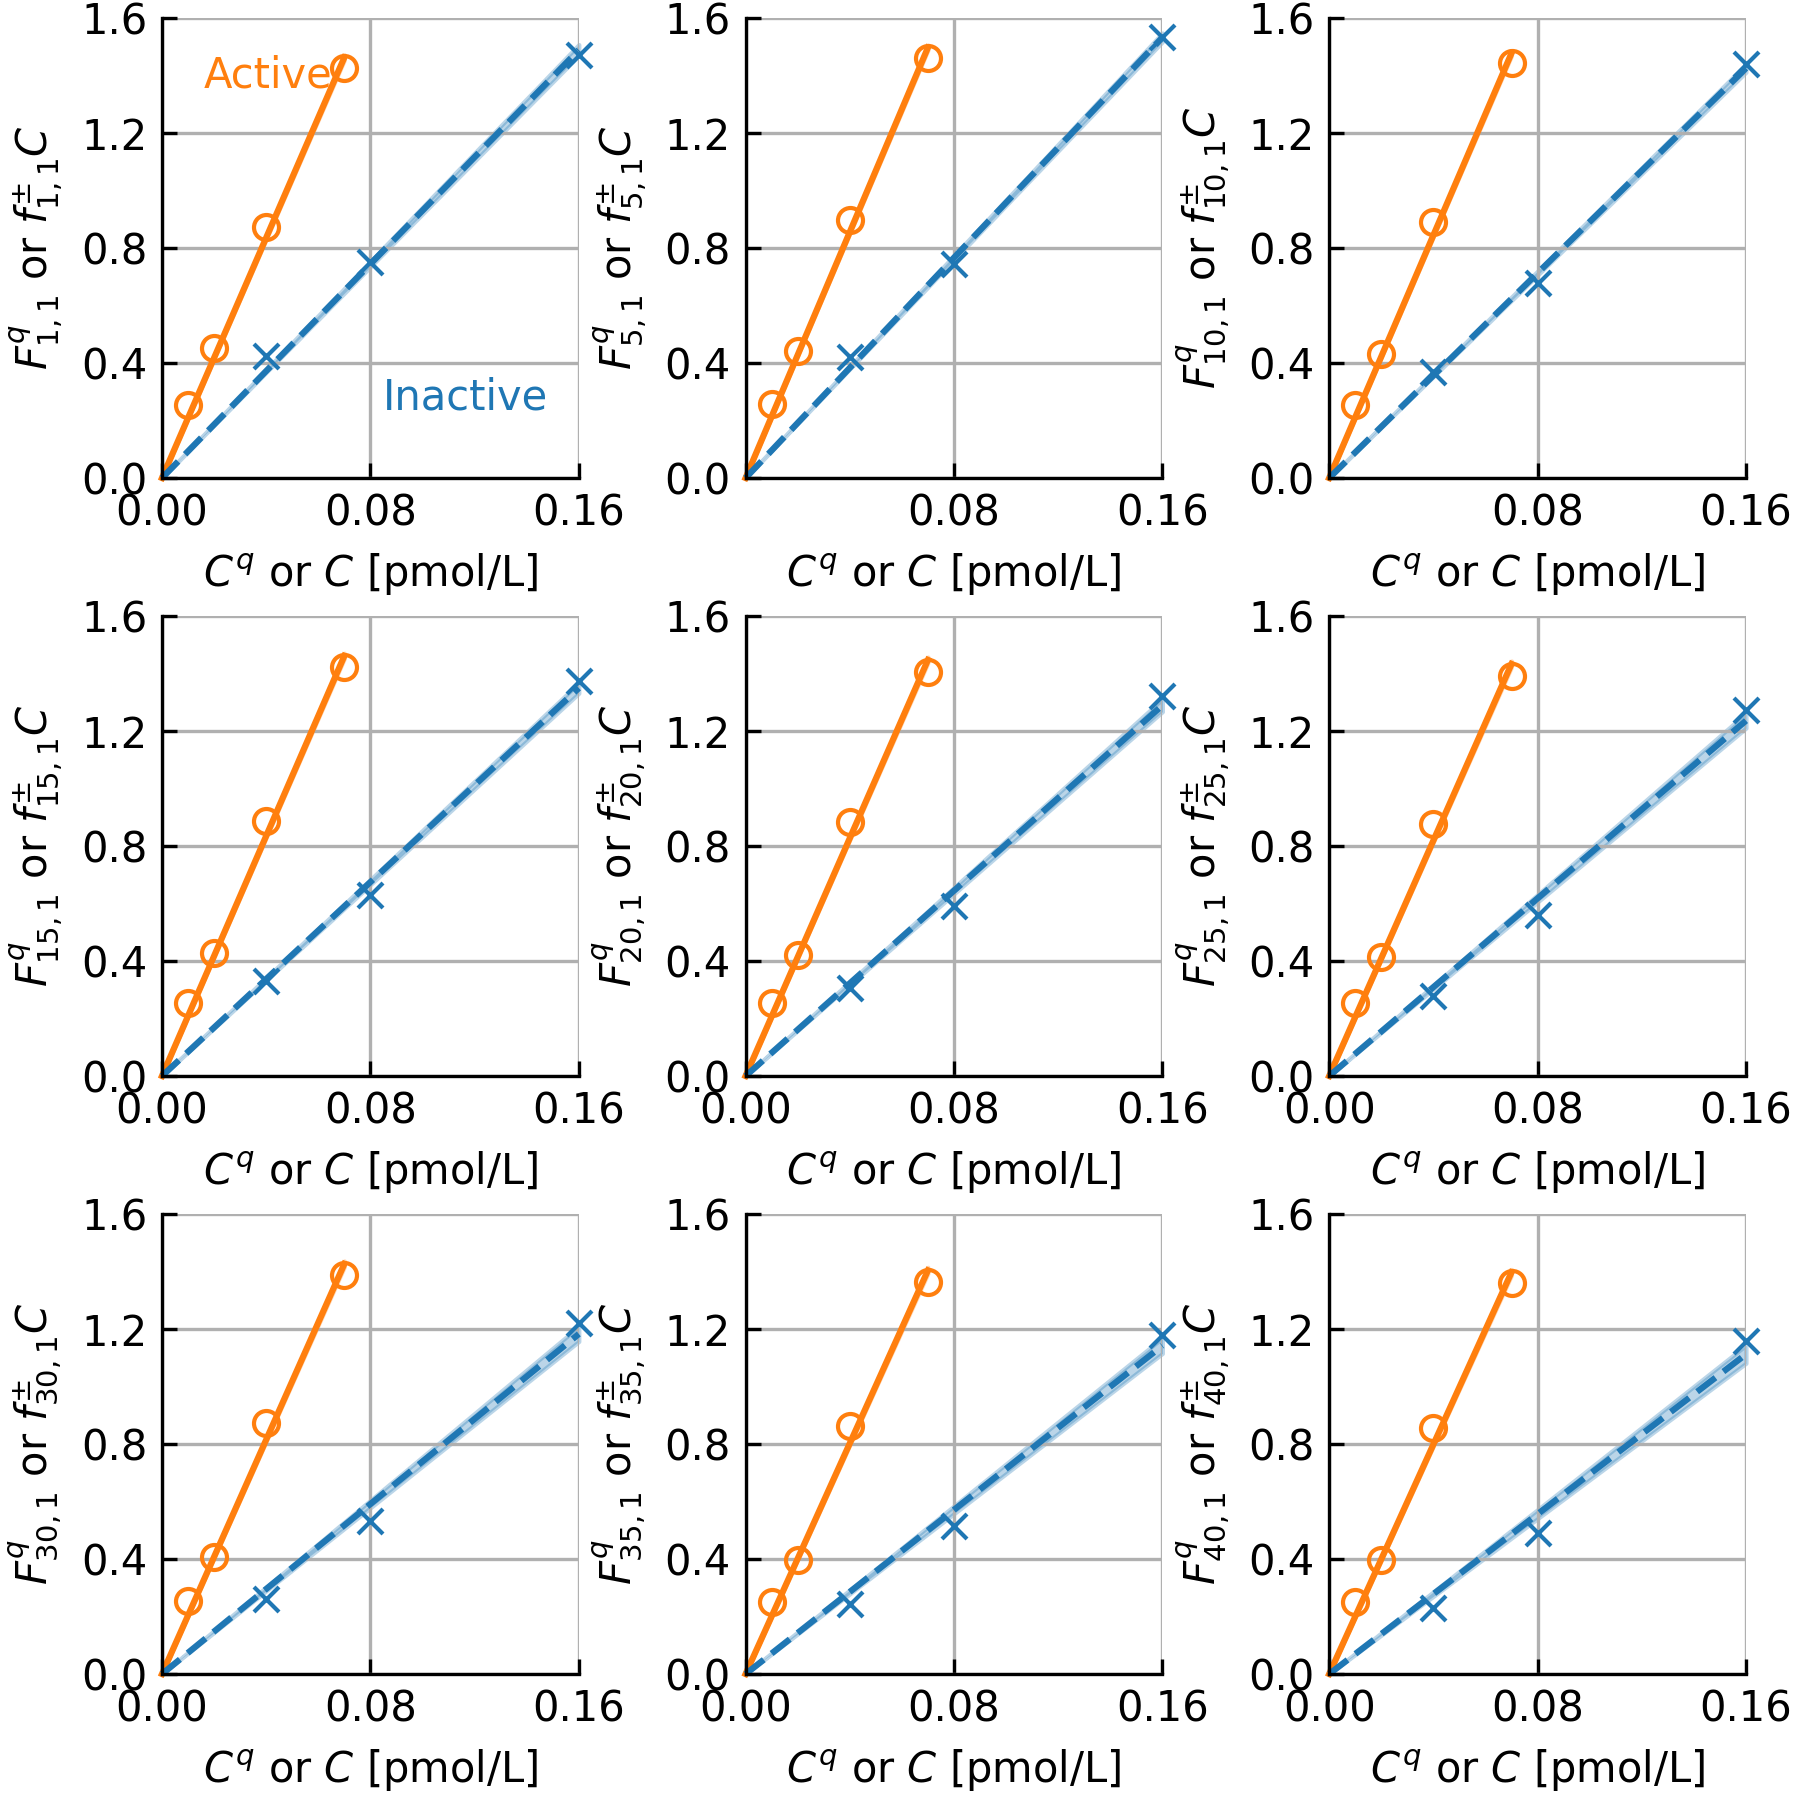
\includegraphics{si-figs/FigS1.png}
                \caption{
                    Experimental data points (symbols, $(C^\ell, F_{i,1}^\ell)$ for each $\ell = 1$ to $q$
                    at fixed cycle $i$)
                    compared to model for inactive probe (blue, dashed lines)
                    and active probe (orange, straight lines).
                    The subplots depict cycles $i=1, 5, 10, 15, 20, 25, 30,$ and 40
                    in left-to-right and top-to-bottom order.
                    Well $w=1$ is also called well A1.
                }
                \label{fig:S1}
            \end{figure}
            \clearpage
            
    \begin{table}
        \caption{Molar Fluorescence Parameters for Well A1 ($w=1$)}
        \centering
        \begin{tabular}{c|ll|ll}
            Cycle & \multicolumn{2}{c|}{Inactive} & \multicolumn{2}{c}{Active} \\
            \hline
            $i$ & $f_{i,1}^{-}$ & $\sigma_{i,1}^{-}$ &  $f_{i,1}^{+}$ & $\sigma_{i,1}^{+}$ \\
            \hline
    1 & 9.30 & 0.039 & 20.90 & 0.044 \\
2 & 9.59 & 0.036 & 21.13 & 0.037 \\
3 & 9.76 & 0.035 & 21.39 & 0.039 \\
4 & 9.70 & 0.033 & 21.39 & 0.041 \\
5 & 9.58 & 0.032 & 21.39 & 0.041 \\
6 & 9.42 & 0.030 & 21.34 & 0.042 \\
7 & 9.29 & 0.028 & 21.27 & 0.042 \\
8 & 9.16 & 0.029 & 21.22 & 0.042 \\
9 & 9.02 & 0.029 & 21.18 & 0.042 \\
10 & 8.91 & 0.029 & 21.11 & 0.043 \\
11 & 8.77 & 0.030 & 21.01 & 0.043 \\
12 & 8.67 & 0.031 & 21.00 & 0.043 \\
13 & 8.59 & 0.033 & 20.99 & 0.043 \\
14 & 8.51 & 0.035 & 20.93 & 0.043 \\
15 & 8.43 & 0.037 & 20.88 & 0.045 \\
16 & 8.34 & 0.037 & 20.83 & 0.046 \\
17 & 8.29 & 0.042 & 20.82 & 0.048 \\
18 & 8.19 & 0.042 & 20.79 & 0.047 \\
19 & 8.11 & 0.041 & 20.75 & 0.047 \\
20 & 8.06 & 0.046 & 20.68 & 0.048 \\
21 & 7.99 & 0.049 & 20.72 & 0.046 \\
22 & 7.87 & 0.046 & 20.66 & 0.048 \\
23 & 7.82 & 0.048 & 20.65 & 0.048 \\
24 & 7.74 & 0.050 & 20.54 & 0.050 \\
25 & 7.73 & 0.054 & 20.48 & 0.049 \\
26 & 7.63 & 0.053 & 20.47 & 0.049 \\
27 & 7.57 & 0.049 & 20.45 & 0.050 \\
28 & 7.53 & 0.053 & 20.39 & 0.050 \\
29 & 7.50 & 0.055 & 20.48 & 0.048 \\
30 & 7.39 & 0.054 & 20.38 & 0.049 \\
31 & 7.33 & 0.054 & 20.32 & 0.049 \\
32 & 7.26 & 0.054 & 20.38 & 0.049 \\
33 & 7.22 & 0.054 & 20.32 & 0.049 \\
34 & 7.19 & 0.055 & 20.19 & 0.049 \\
35 & 7.14 & 0.056 & 20.06 & 0.051 \\
36 & 7.08 & 0.060 & 20.09 & 0.049 \\
37 & 7.06 & 0.060 & 20.07 & 0.050 \\
38 & 7.03 & 0.062 & 20.02 & 0.049 \\
39 & 6.99 & 0.064 & 19.98 & 0.048 \\
40 & 6.95 & 0.065 & 19.96 & 0.048 \\
41 & 6.92 & 0.067 & 19.85 & 0.051 \\
42 & 6.75 & 0.064 & 19.81 & 0.047 \\
43 & 6.72 & 0.068 & 19.80 & 0.044 \\
44 & 6.70 & 0.071 & 19.76 & 0.045 \\
45 & 6.56 & 0.065 & 19.76 & 0.046 \\
               \hline
        \end{tabular}
    \end{table}
    \clearpage

                \begin{figure}
                    \centering
                    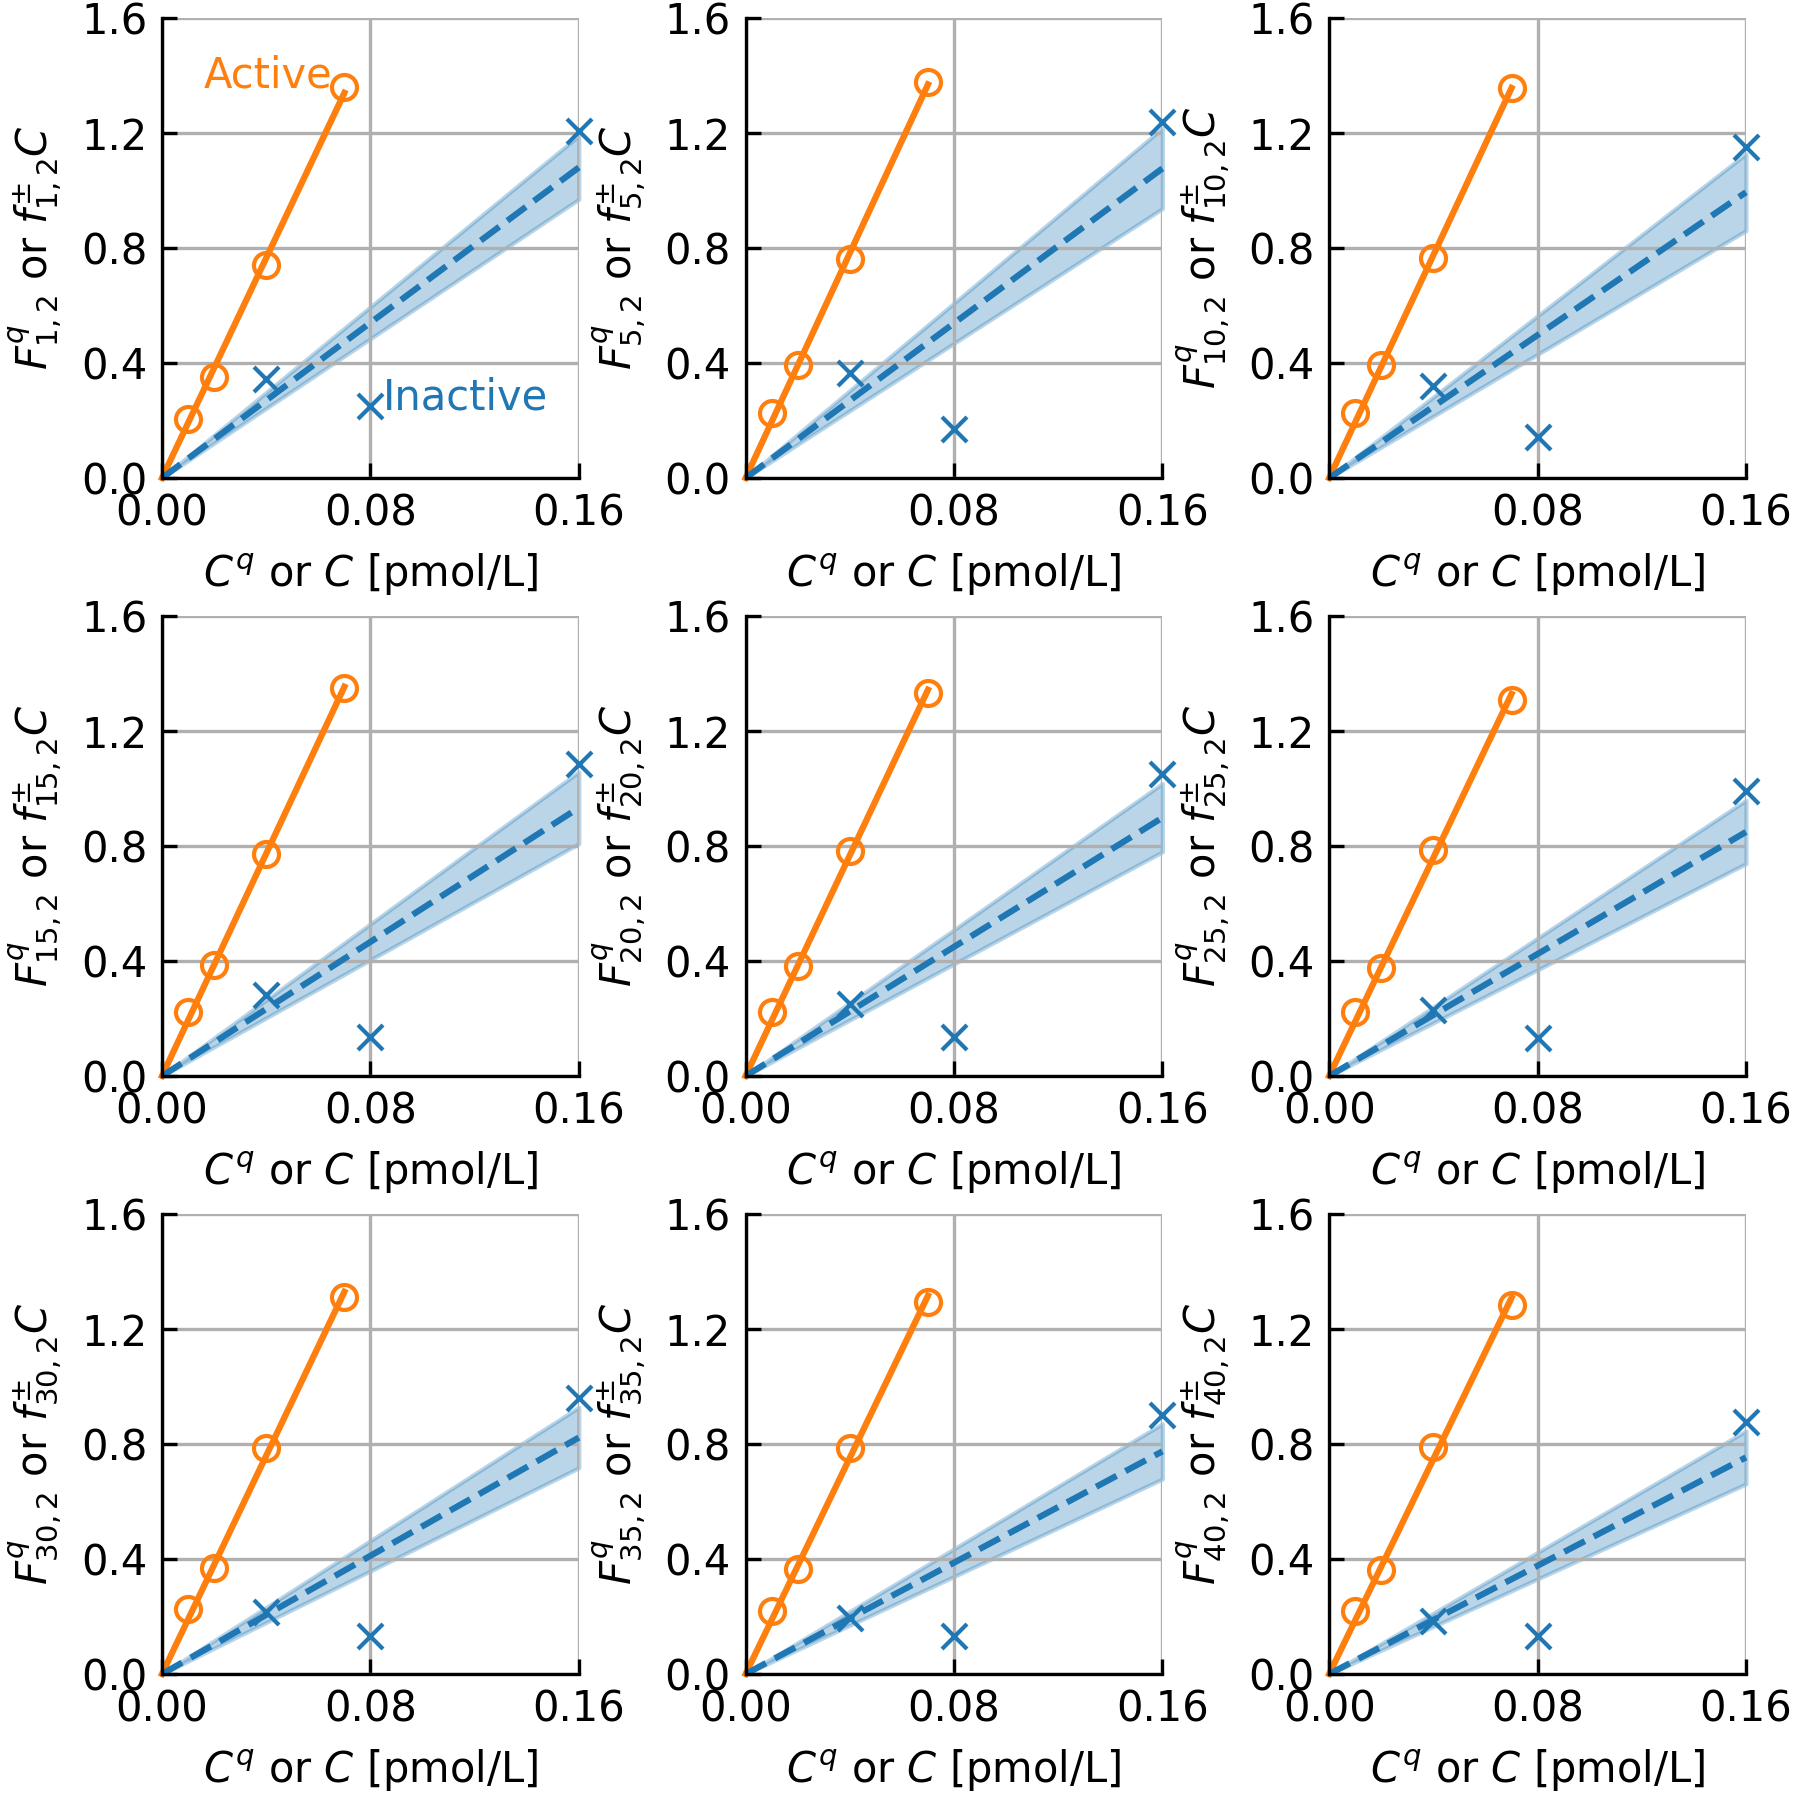
\includegraphics{si-figs/FigS2.png}
                    \caption{
                        As Figure~\ref{fig:S1} with well $w=2$ (or A2).
                    }
                \end{figure}
                \clearpage
    \begin{table}
        \caption{Molar Fluorescence Parameters for Well A2 ($w=2$)}
        \centering
        \begin{tabular}{c|ll|ll}
            Cycle & \multicolumn{2}{c|}{Inactive} & \multicolumn{2}{c}{Active} \\
            \hline
            $i$ & $f_{i,2}^{-}$ & $\sigma_{i,2}^{-}$ &  $f_{i,2}^{+}$ & $\sigma_{i,2}^{+}$ \\
            \hline
    1 & 6.8 & 0.23 & 19.14 & 0.027 \\
2 & 6.8 & 0.26 & 19.22 & 0.024 \\
3 & 6.9 & 0.28 & 19.47 & 0.024 \\
4 & 6.8 & 0.29 & 19.56 & 0.023 \\
5 & 6.7 & 0.29 & 19.56 & 0.022 \\
6 & 6.6 & 0.29 & 19.55 & 0.022 \\
7 & 6.5 & 0.29 & 19.51 & 0.021 \\
8 & 6.4 & 0.29 & 19.45 & 0.021 \\
9 & 6.3 & 0.28 & 19.42 & 0.020 \\
10 & 6.2 & 0.28 & 19.38 & 0.019 \\
11 & 6.1 & 0.27 & 19.42 & 0.019 \\
12 & 6.0 & 0.27 & 19.37 & 0.019 \\
13 & 6.0 & 0.27 & 19.34 & 0.018 \\
14 & 5.9 & 0.26 & 19.32 & 0.018 \\
15 & 5.8 & 0.26 & 19.34 & 0.018 \\
16 & 5.8 & 0.26 & 19.32 & 0.018 \\
17 & 5.7 & 0.25 & 19.23 & 0.019 \\
18 & 5.7 & 0.25 & 19.27 & 0.020 \\
19 & 5.6 & 0.25 & 19.21 & 0.020 \\
20 & 5.6 & 0.25 & 19.19 & 0.021 \\
21 & 5.5 & 0.24 & 19.17 & 0.021 \\
22 & 5.5 & 0.24 & 19.13 & 0.022 \\
23 & 5.4 & 0.23 & 19.15 & 0.023 \\
24 & 5.4 & 0.23 & 19.10 & 0.024 \\
25 & 5.3 & 0.23 & 18.99 & 0.028 \\
26 & 5.3 & 0.23 & 19.06 & 0.027 \\
27 & 5.3 & 0.23 & 18.97 & 0.026 \\
28 & 5.2 & 0.23 & 19.01 & 0.027 \\
29 & 5.2 & 0.22 & 19.00 & 0.027 \\
30 & 5.1 & 0.22 & 18.99 & 0.028 \\
31 & 5.0 & 0.21 & 18.96 & 0.025 \\
32 & 4.9 & 0.21 & 18.88 & 0.026 \\
33 & 4.9 & 0.20 & 18.77 & 0.030 \\
34 & 4.9 & 0.20 & 18.80 & 0.029 \\
35 & 4.8 & 0.20 & 18.80 & 0.030 \\
36 & 4.8 & 0.20 & 18.80 & 0.031 \\
37 & 4.8 & 0.20 & 18.71 & 0.033 \\
38 & 4.8 & 0.20 & 18.75 & 0.032 \\
39 & 4.7 & 0.19 & 18.72 & 0.033 \\
40 & 4.7 & 0.19 & 18.70 & 0.034 \\
41 & 4.7 & 0.19 & 18.68 & 0.036 \\
42 & 4.7 & 0.19 & 18.60 & 0.036 \\
43 & 4.6 & 0.19 & 18.58 & 0.037 \\
44 & 4.6 & 0.19 & 18.59 & 0.038 \\
45 & 4.6 & 0.18 & 18.56 & 0.038 \\
               \hline
        \end{tabular}
    \end{table}
    \clearpage

                \begin{figure}
                    \centering
                    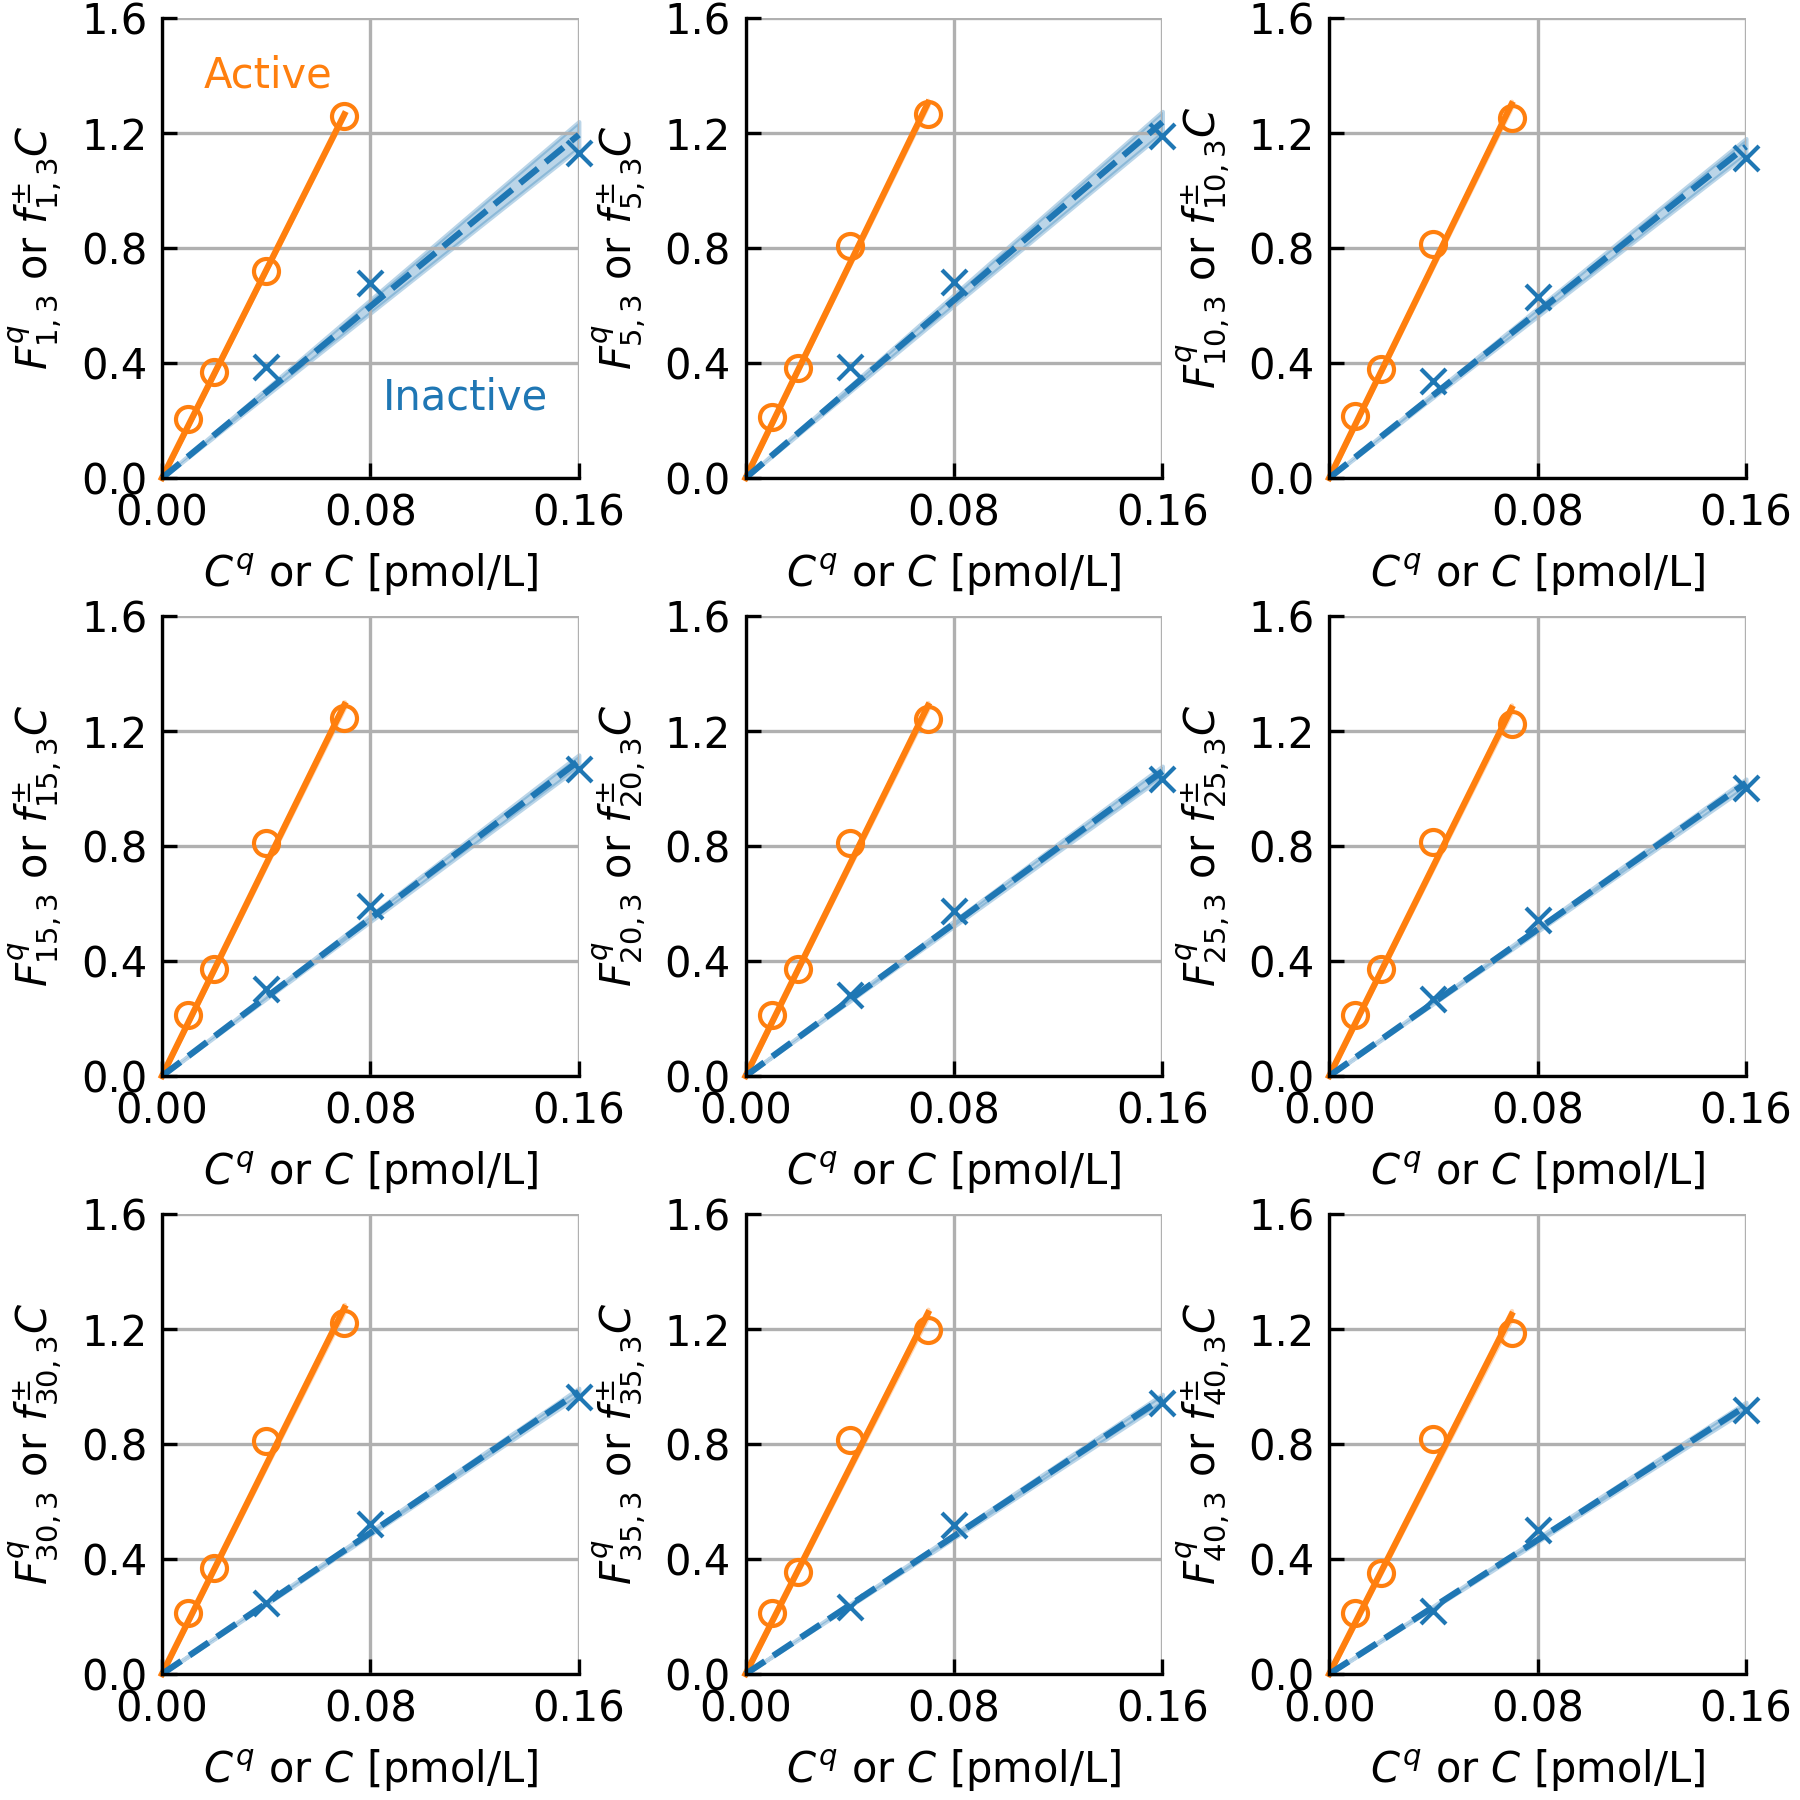
\includegraphics{si-figs/FigS3.png}
                    \caption{
                        As Figure~\ref{fig:S1} with well $w=3$ (or A3).
                    }
                \end{figure}
                \clearpage
    \begin{table}
        \caption{Molar Fluorescence Parameters for Well A3 ($w=3$)}
        \centering
        \begin{tabular}{c|ll|ll}
            Cycle & \multicolumn{2}{c|}{Inactive} & \multicolumn{2}{c}{Active} \\
            \hline
            $i$ & $f_{i,3}^{-}$ & $\sigma_{i,3}^{-}$ &  $f_{i,3}^{+}$ & $\sigma_{i,3}^{+}$ \\
            \hline
    1 & 7.46 & 0.095 & 18.07 & 0.015 \\
2 & 7.73 & 0.085 & 18.16 & 0.032 \\
3 & 7.84 & 0.086 & 18.46 & 0.041 \\
4 & 7.81 & 0.083 & 18.61 & 0.042 \\
5 & 7.74 & 0.078 & 18.64 & 0.045 \\
6 & 7.63 & 0.074 & 18.65 & 0.047 \\
7 & 7.51 & 0.069 & 18.64 & 0.049 \\
8 & 7.41 & 0.064 & 18.62 & 0.050 \\
9 & 7.31 & 0.061 & 18.59 & 0.051 \\
10 & 7.21 & 0.058 & 18.57 & 0.052 \\
11 & 7.13 & 0.053 & 18.54 & 0.052 \\
12 & 7.06 & 0.050 & 18.52 & 0.052 \\
13 & 6.99 & 0.048 & 18.48 & 0.053 \\
14 & 6.93 & 0.044 & 18.48 & 0.053 \\
15 & 6.85 & 0.043 & 18.44 & 0.053 \\
16 & 6.81 & 0.041 & 18.47 & 0.054 \\
17 & 6.74 & 0.041 & 18.57 & 0.050 \\
18 & 6.69 & 0.038 & 18.47 & 0.053 \\
19 & 6.64 & 0.037 & 18.41 & 0.054 \\
20 & 6.62 & 0.038 & 18.40 & 0.054 \\
21 & 6.54 & 0.036 & 18.37 & 0.057 \\
22 & 6.49 & 0.033 & 18.30 & 0.059 \\
23 & 6.49 & 0.030 & 18.24 & 0.060 \\
24 & 6.44 & 0.029 & 18.41 & 0.055 \\
25 & 6.37 & 0.028 & 18.27 & 0.059 \\
26 & 6.40 & 0.026 & 18.24 & 0.063 \\
27 & 6.36 & 0.023 & 18.18 & 0.061 \\
28 & 6.29 & 0.023 & 18.14 & 0.061 \\
29 & 6.18 & 0.026 & 18.09 & 0.062 \\
30 & 6.14 & 0.026 & 18.19 & 0.060 \\
31 & 6.11 & 0.025 & 18.06 & 0.062 \\
32 & 6.07 & 0.023 & 18.01 & 0.065 \\
33 & 6.06 & 0.023 & 17.99 & 0.065 \\
34 & 5.97 & 0.027 & 17.95 & 0.067 \\
35 & 5.99 & 0.029 & 17.93 & 0.067 \\
36 & 5.96 & 0.026 & 17.88 & 0.069 \\
37 & 5.92 & 0.027 & 17.88 & 0.070 \\
38 & 5.89 & 0.026 & 17.87 & 0.072 \\
39 & 5.86 & 0.027 & 17.96 & 0.078 \\
40 & 5.83 & 0.027 & 17.85 & 0.073 \\
41 & 5.80 & 0.029 & 17.86 & 0.072 \\
42 & 5.74 & 0.030 & 17.82 & 0.073 \\
43 & 5.67 & 0.031 & 17.78 & 0.076 \\
44 & 5.64 & 0.032 & 17.70 & 0.076 \\
45 & 5.62 & 0.033 & 17.70 & 0.076 \\
               \hline
        \end{tabular}
    \end{table}
    \clearpage

                \begin{figure}
                    \centering
                    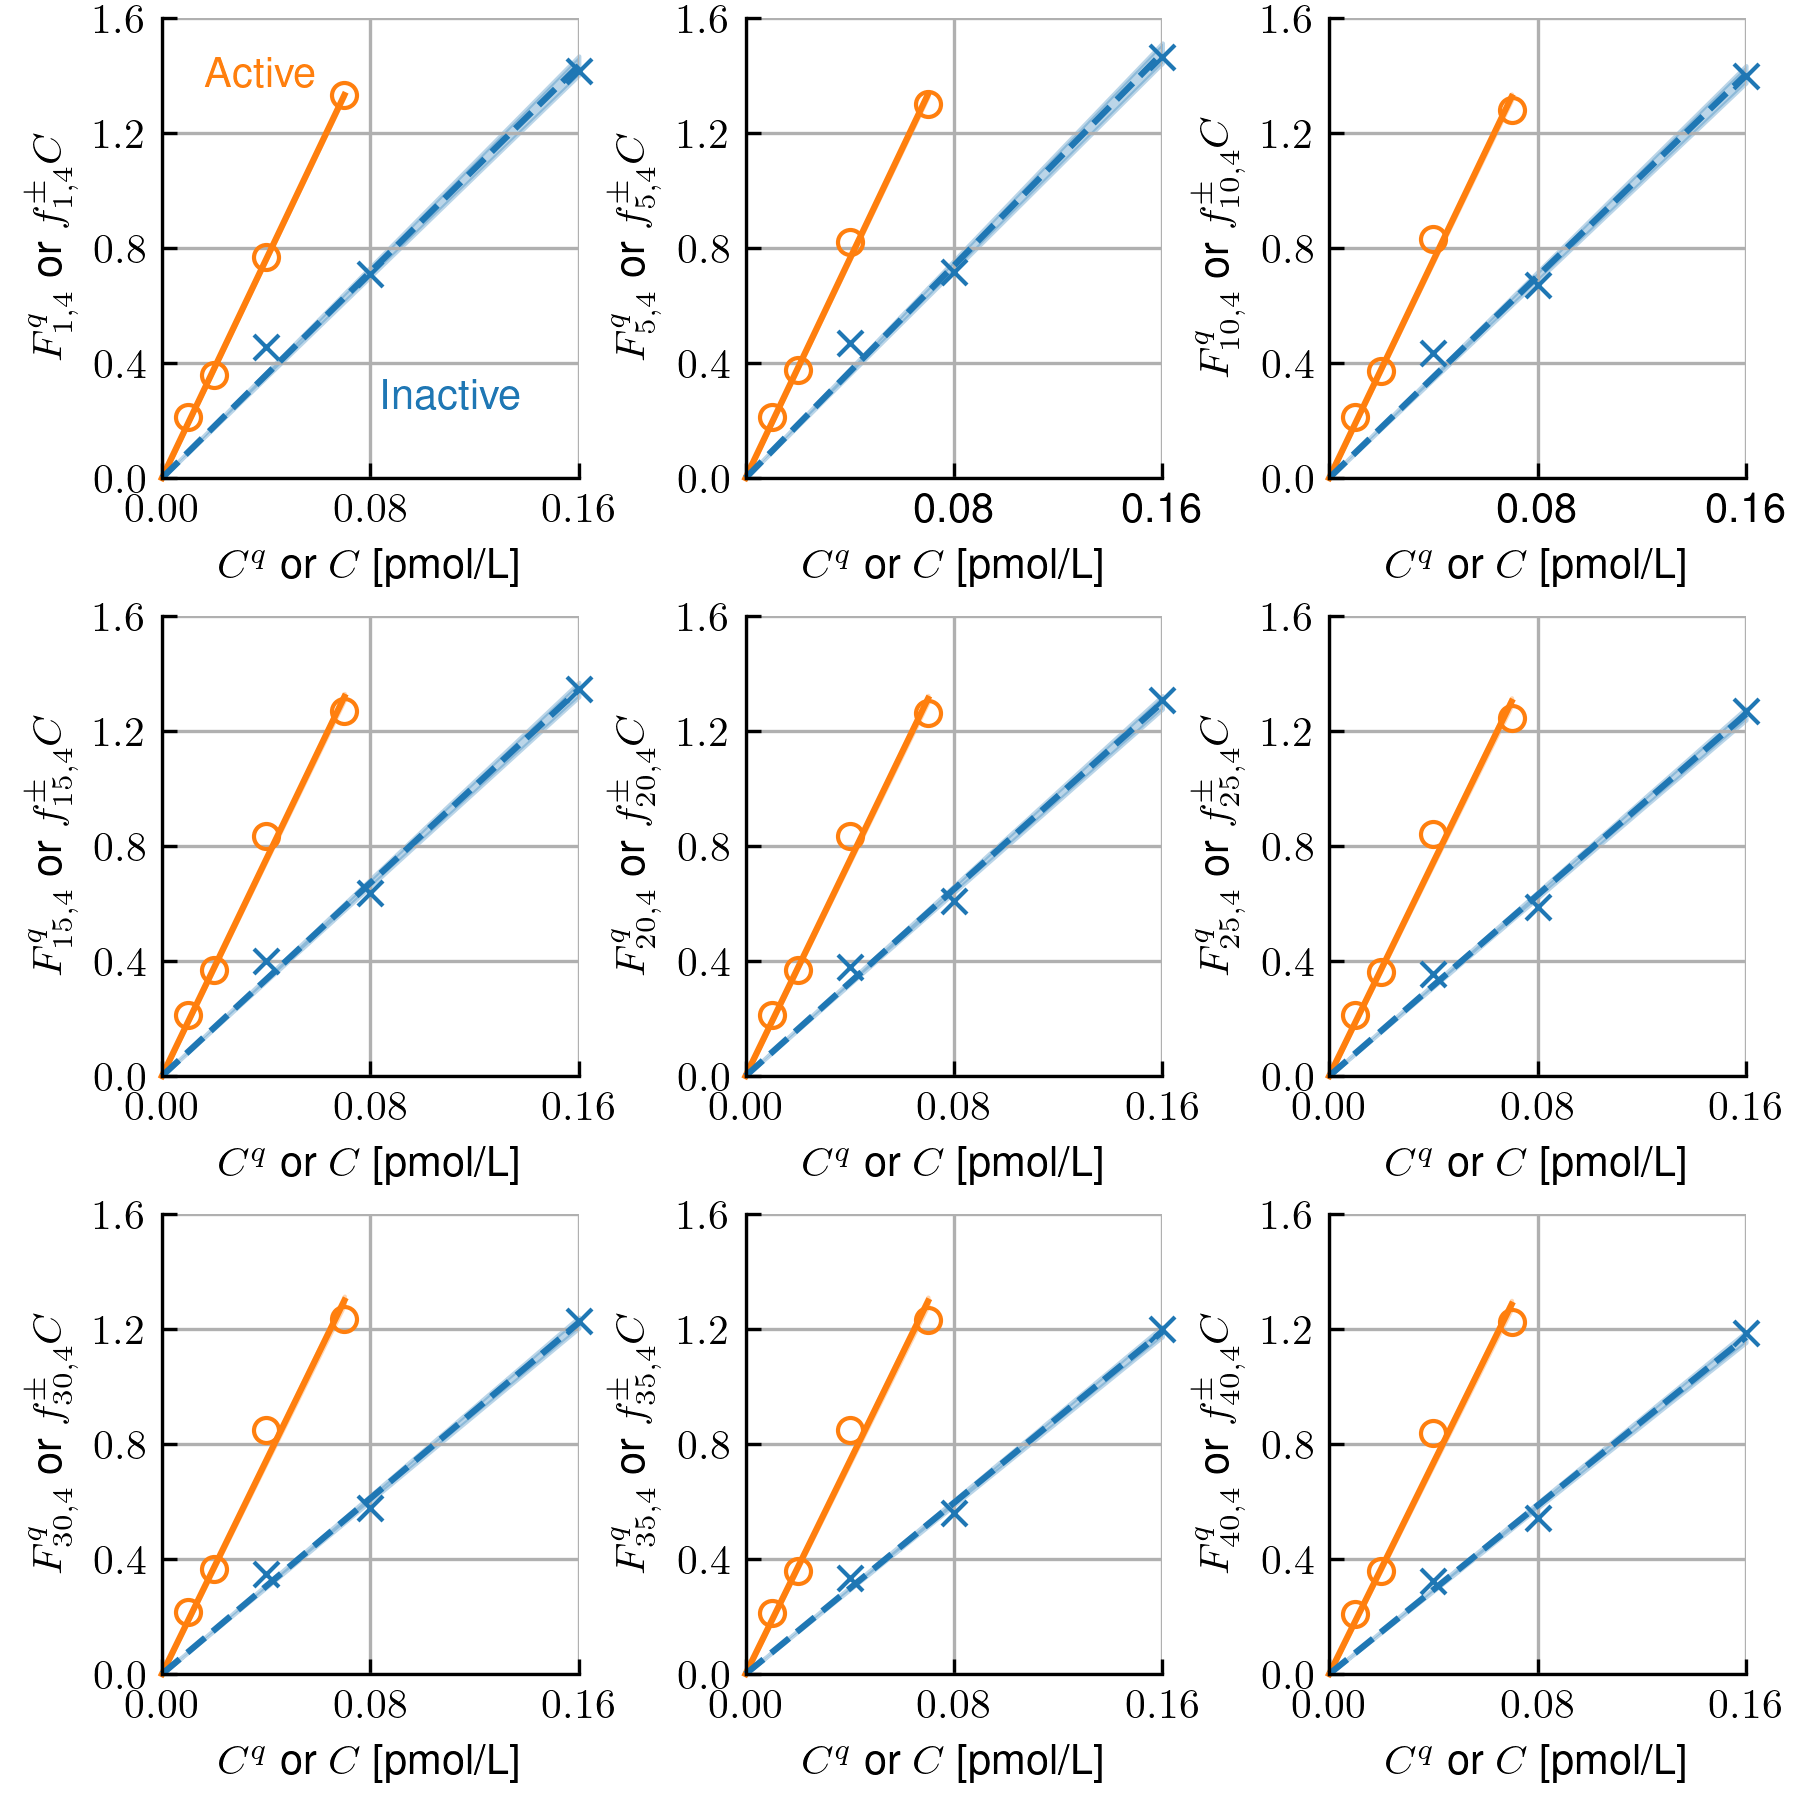
\includegraphics{si-figs/FigS4.png}
                    \caption{
                        As Figure~\ref{fig:S1} with well $w=4$ (or A4).
                    }
                \end{figure}
                \clearpage
    \begin{table}
        \caption{Molar Fluorescence Parameters for Well A4 ($w=4$)}
        \centering
        \begin{tabular}{c|ll|ll}
            Cycle & \multicolumn{2}{c|}{Inactive} & \multicolumn{2}{c}{Active} \\
            \hline
            $i$ & $f_{i,4}^{-}$ & $\sigma_{i,4}^{-}$ &  $f_{i,4}^{+}$ & $\sigma_{i,4}^{+}$ \\
            \hline
    1 & 8.97 & 0.070 & 19.03 & 0.018 \\
2 & 9.10 & 0.075 & 18.75 & 0.026 \\
3 & 9.27 & 0.075 & 18.92 & 0.032 \\
4 & 9.30 & 0.074 & 19.02 & 0.037 \\
5 & 9.24 & 0.073 & 19.06 & 0.041 \\
6 & 9.16 & 0.071 & 19.05 & 0.044 \\
7 & 9.06 & 0.069 & 19.01 & 0.048 \\
8 & 8.98 & 0.067 & 18.99 & 0.050 \\
9 & 8.87 & 0.065 & 18.95 & 0.050 \\
10 & 8.78 & 0.063 & 18.93 & 0.052 \\
11 & 8.70 & 0.061 & 18.91 & 0.054 \\
12 & 8.62 & 0.058 & 18.85 & 0.052 \\
13 & 8.56 & 0.056 & 18.89 & 0.054 \\
14 & 8.47 & 0.054 & 18.88 & 0.056 \\
15 & 8.40 & 0.053 & 18.84 & 0.057 \\
16 & 8.32 & 0.051 & 18.85 & 0.055 \\
17 & 8.26 & 0.048 & 18.81 & 0.058 \\
18 & 8.20 & 0.048 & 18.79 & 0.059 \\
19 & 8.23 & 0.051 & 18.74 & 0.059 \\
20 & 8.12 & 0.049 & 18.74 & 0.058 \\
21 & 8.06 & 0.047 & 18.85 & 0.055 \\
22 & 8.01 & 0.047 & 18.67 & 0.063 \\
23 & 7.98 & 0.046 & 18.65 & 0.065 \\
24 & 7.91 & 0.045 & 18.63 & 0.064 \\
25 & 7.87 & 0.043 & 18.60 & 0.067 \\
26 & 7.83 & 0.044 & 18.69 & 0.066 \\
27 & 7.79 & 0.042 & 18.63 & 0.067 \\
28 & 7.73 & 0.042 & 18.56 & 0.071 \\
29 & 7.70 & 0.040 & 18.55 & 0.072 \\
30 & 7.64 & 0.040 & 18.56 & 0.074 \\
31 & 7.61 & 0.037 & 18.56 & 0.071 \\
32 & 7.52 & 0.033 & 18.51 & 0.077 \\
33 & 7.50 & 0.032 & 18.47 & 0.077 \\
34 & 7.49 & 0.034 & 18.44 & 0.072 \\
35 & 7.44 & 0.036 & 18.51 & 0.074 \\
36 & 7.45 & 0.030 & 18.36 & 0.077 \\
37 & 7.41 & 0.035 & 18.39 & 0.075 \\
38 & 7.38 & 0.036 & 18.37 & 0.075 \\
39 & 7.35 & 0.035 & 18.35 & 0.076 \\
40 & 7.32 & 0.039 & 18.35 & 0.073 \\
41 & 7.29 & 0.038 & 18.32 & 0.075 \\
42 & 7.30 & 0.033 & 18.37 & 0.072 \\
43 & 7.28 & 0.036 & 18.21 & 0.078 \\
44 & 7.25 & 0.034 & 18.14 & 0.076 \\
45 & 7.24 & 0.039 & 18.13 & 0.077 \\
               \hline
        \end{tabular}
    \end{table}
    \clearpage

                \begin{figure}
                    \centering
                    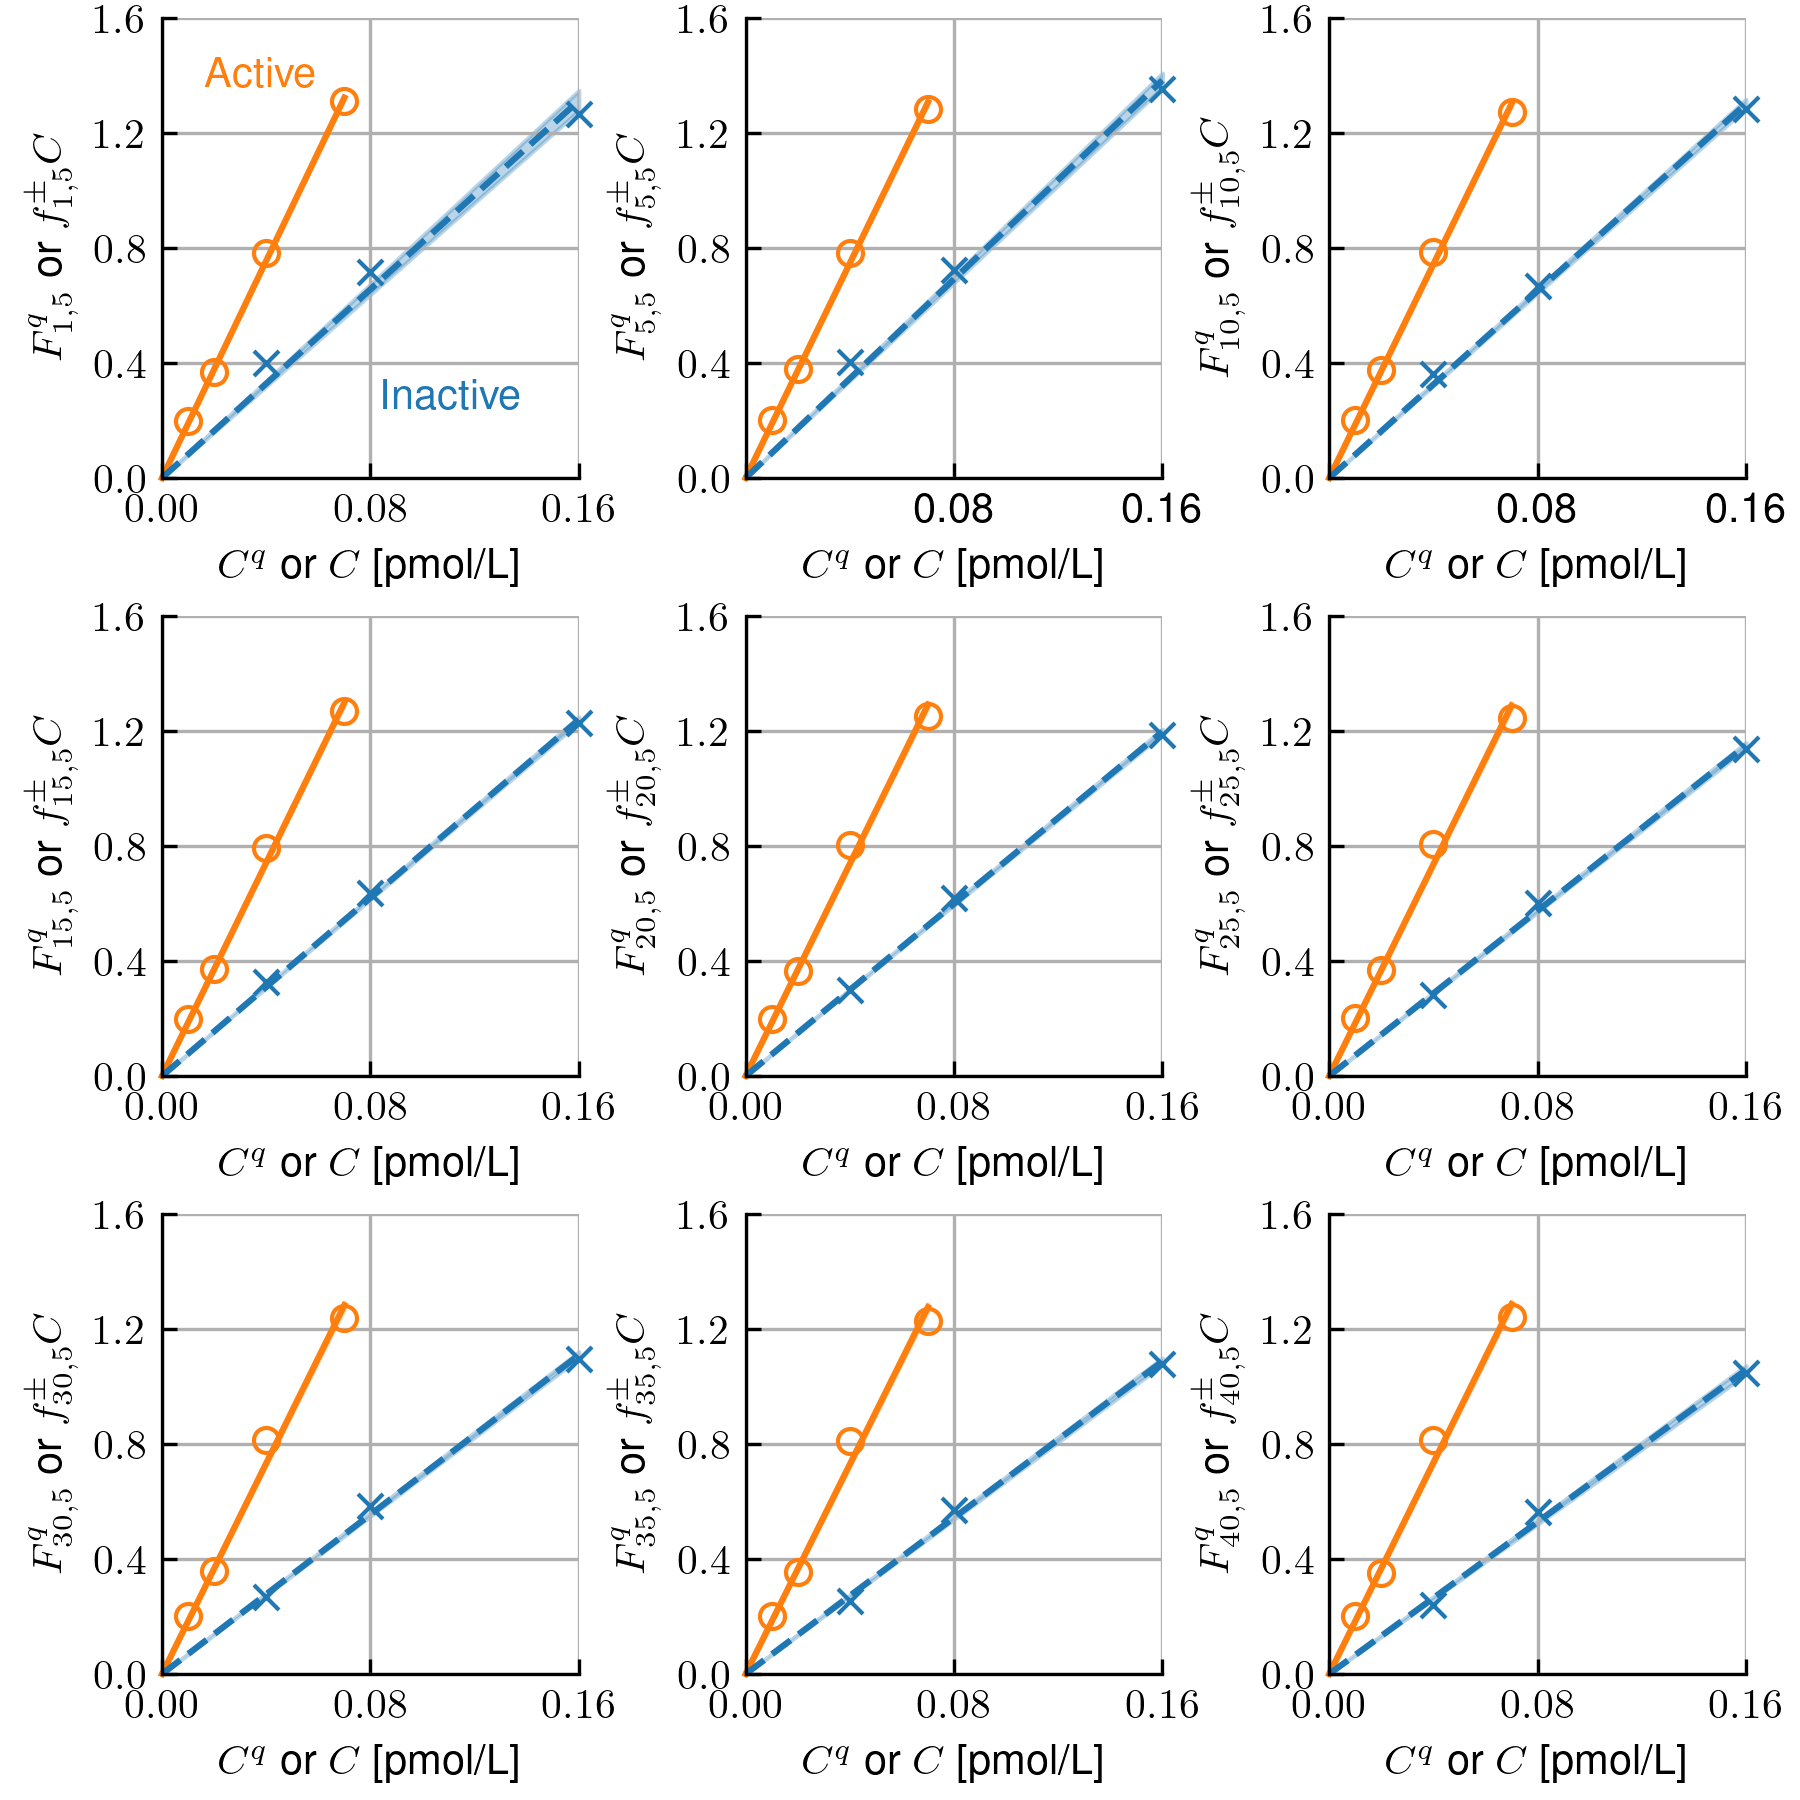
\includegraphics{si-figs/FigS5.png}
                    \caption{
                        As Figure~\ref{fig:S1} with well $w=5$ (or A5).
                    }
                \end{figure}
                \clearpage
    \begin{table}
        \caption{Molar Fluorescence Parameters for Well A5 ($w=5$)}
        \centering
        \begin{tabular}{c|ll|ll}
            Cycle & \multicolumn{2}{c|}{Inactive} & \multicolumn{2}{c}{Active} \\
            \hline
            $i$ & $f_{i,5}^{-}$ & $\sigma_{i,5}^{-}$ &  $f_{i,5}^{+}$ & $\sigma_{i,5}^{+}$ \\
            \hline
    1 & 8.20 & 0.073 & 18.90 & 0.019 \\
2 & 8.41 & 0.063 & 18.40 & 0.022 \\
3 & 8.66 & 0.056 & 18.55 & 0.023 \\
4 & 8.70 & 0.054 & 18.62 & 0.025 \\
5 & 8.64 & 0.052 & 18.67 & 0.026 \\
6 & 8.56 & 0.050 & 18.67 & 0.027 \\
7 & 8.46 & 0.046 & 18.69 & 0.028 \\
8 & 8.35 & 0.043 & 18.63 & 0.029 \\
9 & 8.24 & 0.039 & 18.62 & 0.030 \\
10 & 8.14 & 0.032 & 18.59 & 0.030 \\
11 & 8.04 & 0.029 & 18.57 & 0.031 \\
12 & 7.96 & 0.027 & 18.55 & 0.029 \\
13 & 7.89 & 0.024 & 18.55 & 0.030 \\
14 & 7.82 & 0.021 & 18.58 & 0.033 \\
15 & 7.75 & 0.019 & 18.56 & 0.035 \\
16 & 7.70 & 0.017 & 18.55 & 0.038 \\
17 & 7.66 & 0.017 & 18.54 & 0.039 \\
18 & 7.58 & 0.018 & 18.51 & 0.043 \\
19 & 7.52 & 0.019 & 18.51 & 0.043 \\
20 & 7.49 & 0.017 & 18.45 & 0.045 \\
21 & 7.43 & 0.018 & 18.43 & 0.046 \\
22 & 7.40 & 0.017 & 18.41 & 0.046 \\
23 & 7.31 & 0.019 & 18.44 & 0.047 \\
24 & 7.23 & 0.021 & 18.38 & 0.048 \\
25 & 7.18 & 0.021 & 18.41 & 0.049 \\
26 & 7.12 & 0.022 & 18.40 & 0.050 \\
27 & 7.07 & 0.024 & 18.45 & 0.049 \\
28 & 7.04 & 0.022 & 18.38 & 0.052 \\
29 & 6.99 & 0.023 & 18.35 & 0.052 \\
30 & 6.93 & 0.023 & 18.33 & 0.055 \\
31 & 6.89 & 0.025 & 18.29 & 0.056 \\
32 & 6.86 & 0.024 & 18.26 & 0.053 \\
33 & 6.81 & 0.026 & 18.22 & 0.055 \\
34 & 6.82 & 0.027 & 18.21 & 0.056 \\
35 & 6.80 & 0.025 & 18.23 & 0.056 \\
36 & 6.78 & 0.025 & 18.19 & 0.057 \\
37 & 6.75 & 0.031 & 18.27 & 0.054 \\
38 & 6.72 & 0.038 & 18.21 & 0.056 \\
39 & 6.67 & 0.035 & 18.20 & 0.055 \\
40 & 6.61 & 0.032 & 18.37 & 0.054 \\
41 & 6.57 & 0.033 & 18.18 & 0.057 \\
42 & 6.51 & 0.028 & 18.18 & 0.056 \\
43 & 6.49 & 0.026 & 18.27 & 0.051 \\
44 & 6.46 & 0.030 & 18.07 & 0.056 \\
45 & 6.43 & 0.030 & 18.01 & 0.059 \\
               \hline
        \end{tabular}
    \end{table}
    \clearpage

                \begin{figure}
                    \centering
                    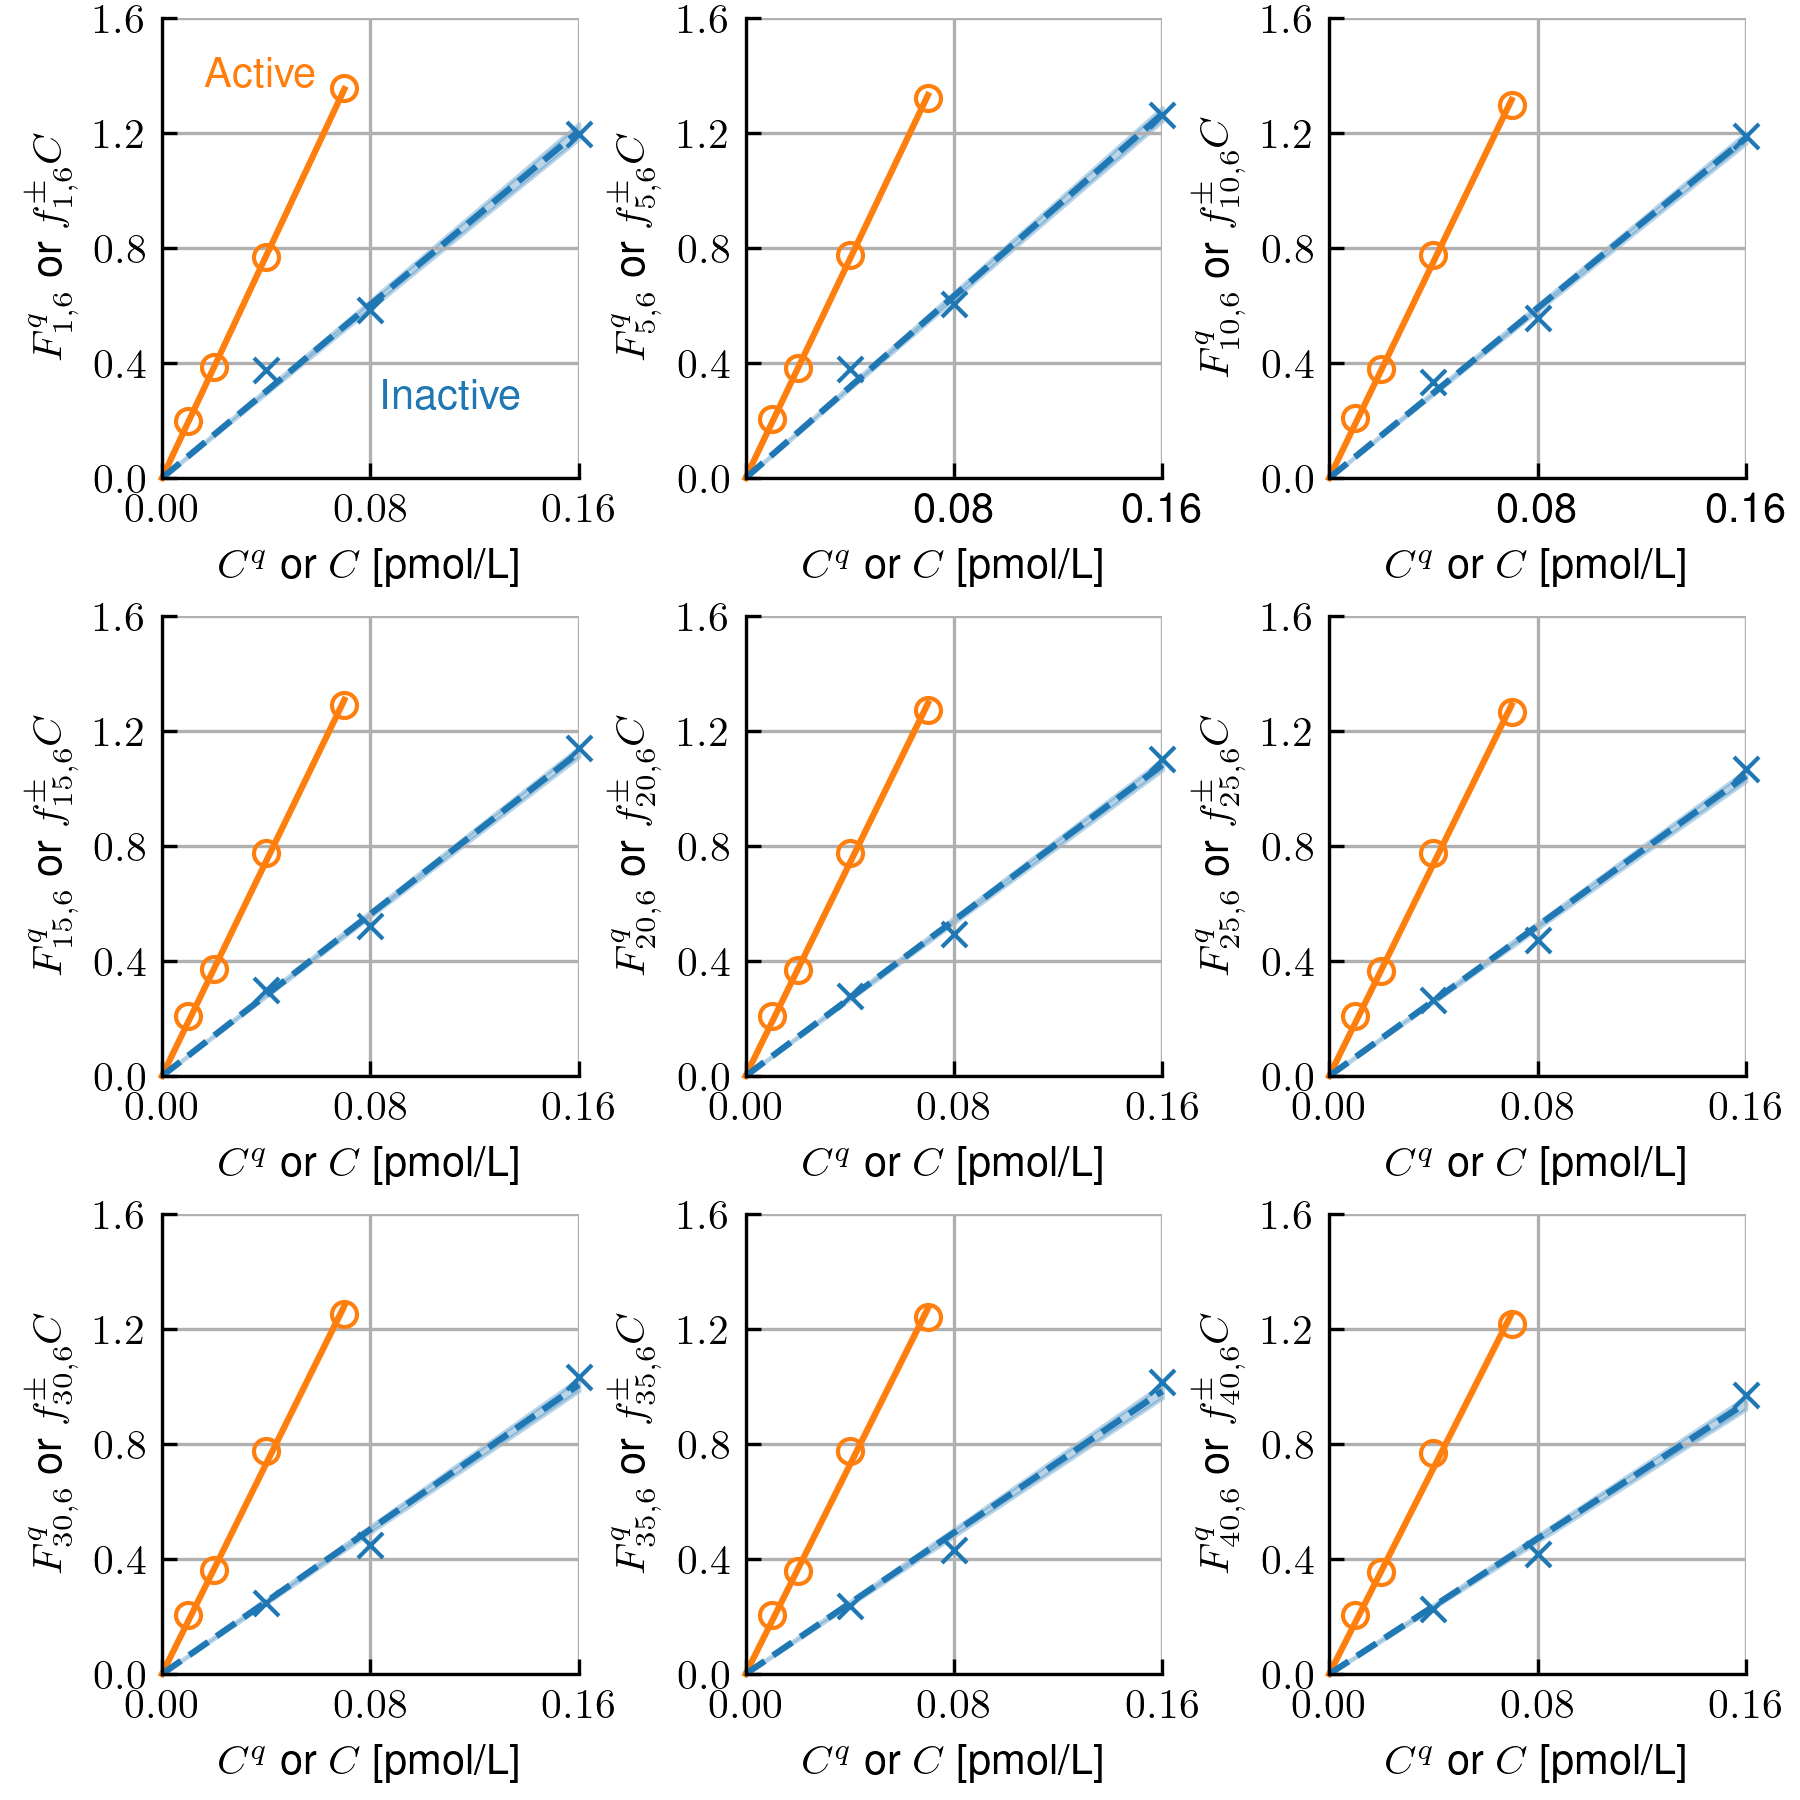
\includegraphics{si-figs/FigS6.png}
                    \caption{
                        As Figure~\ref{fig:S1} with well $w=6$ (or A6).
                    }
                \end{figure}
                \clearpage
    \begin{table}
        \caption{Molar Fluorescence Parameters for Well A6 ($w=6$)}
        \centering
        \begin{tabular}{c|ll|ll}
            Cycle & \multicolumn{2}{c|}{Inactive} & \multicolumn{2}{c}{Active} \\
            \hline
            $i$ & $f_{i,6}^{-}$ & $\sigma_{i,6}^{-}$ &  $f_{i,6}^{+}$ & $\sigma_{i,6}^{+}$ \\
            \hline
    1 & 7.54 & 0.055 & 19.323 & 0.0042 \\
2 & 7.77 & 0.048 & 18.772 & 0.0097 \\
3 & 7.93 & 0.048 & 18.93 & 0.010 \\
4 & 7.96 & 0.048 & 19.02 & 0.013 \\
5 & 7.91 & 0.048 & 19.03 & 0.014 \\
6 & 7.82 & 0.047 & 18.99 & 0.015 \\
7 & 7.70 & 0.044 & 18.92 & 0.017 \\
8 & 7.60 & 0.041 & 18.86 & 0.019 \\
9 & 7.51 & 0.040 & 18.85 & 0.020 \\
10 & 7.39 & 0.038 & 18.79 & 0.021 \\
11 & 7.31 & 0.036 & 18.77 & 0.021 \\
12 & 7.24 & 0.036 & 18.75 & 0.023 \\
13 & 7.18 & 0.035 & 18.74 & 0.023 \\
14 & 7.09 & 0.034 & 18.66 & 0.025 \\
15 & 7.04 & 0.034 & 18.69 & 0.024 \\
16 & 6.97 & 0.033 & 18.61 & 0.025 \\
17 & 6.91 & 0.034 & 18.62 & 0.027 \\
18 & 6.85 & 0.035 & 18.57 & 0.027 \\
19 & 6.79 & 0.035 & 18.55 & 0.028 \\
20 & 6.76 & 0.037 & 18.52 & 0.027 \\
21 & 6.71 & 0.036 & 18.53 & 0.028 \\
22 & 6.66 & 0.036 & 18.60 & 0.030 \\
23 & 6.62 & 0.037 & 18.49 & 0.030 \\
24 & 6.57 & 0.040 & 18.46 & 0.030 \\
25 & 6.53 & 0.038 & 18.43 & 0.030 \\
26 & 6.56 & 0.046 & 18.41 & 0.031 \\
27 & 6.57 & 0.050 & 18.37 & 0.031 \\
28 & 6.43 & 0.046 & 18.36 & 0.031 \\
29 & 6.33 & 0.042 & 18.33 & 0.032 \\
30 & 6.29 & 0.043 & 18.30 & 0.033 \\
31 & 6.27 & 0.045 & 18.28 & 0.032 \\
32 & 6.22 & 0.045 & 18.23 & 0.035 \\
33 & 6.24 & 0.050 & 18.23 & 0.036 \\
34 & 6.16 & 0.047 & 18.21 & 0.036 \\
35 & 6.15 & 0.048 & 18.18 & 0.037 \\
36 & 6.03 & 0.044 & 18.26 & 0.045 \\
37 & 6.00 & 0.043 & 18.00 & 0.039 \\
38 & 5.95 & 0.041 & 17.96 & 0.042 \\
39 & 5.92 & 0.043 & 17.89 & 0.040 \\
40 & 5.89 & 0.044 & 17.90 & 0.040 \\
41 & 5.85 & 0.044 & 17.86 & 0.040 \\
42 & 5.84 & 0.045 & 17.88 & 0.039 \\
43 & 5.80 & 0.044 & 17.83 & 0.040 \\
44 & 5.77 & 0.044 & 17.81 & 0.037 \\
45 & 5.76 & 0.046 & 17.81 & 0.038 \\
               \hline
        \end{tabular}
    \end{table}
    \clearpage

                \begin{figure}
                    \centering
                    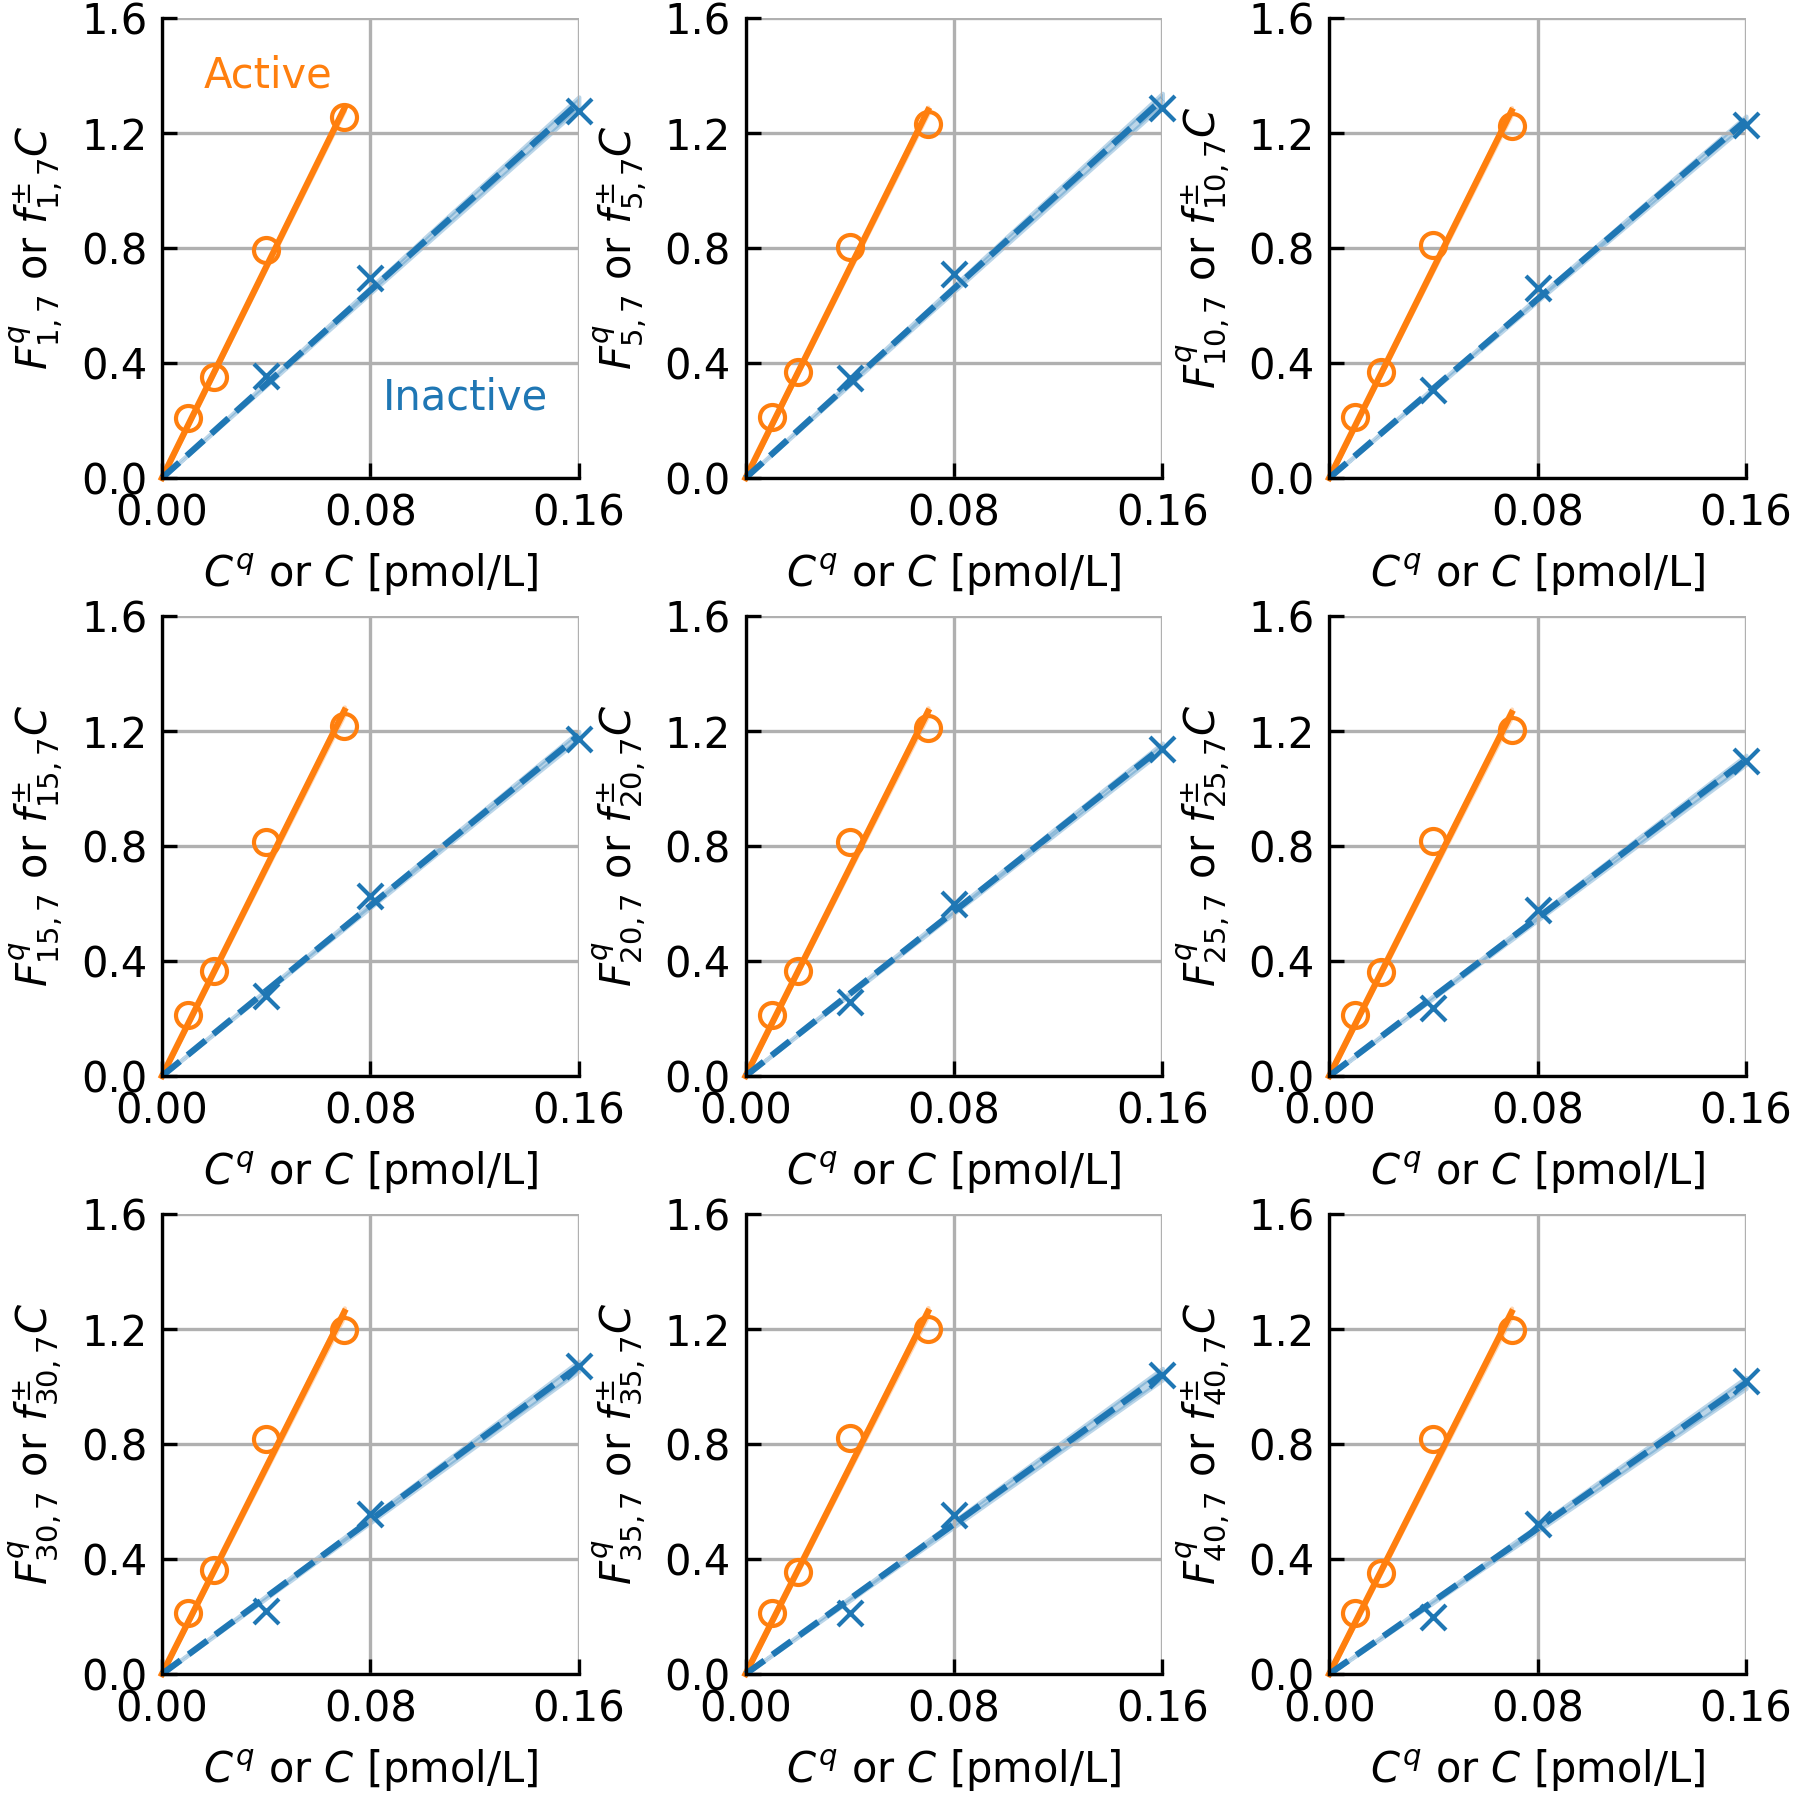
\includegraphics{si-figs/FigS7.png}
                    \caption{
                        As Figure~\ref{fig:S1} with well $w=7$ (or A7).
                    }
                \end{figure}
                \clearpage
    \begin{table}
        \caption{Molar Fluorescence Parameters for Well A7 ($w=7$)}
        \centering
        \begin{tabular}{c|ll|ll}
            Cycle & \multicolumn{2}{c|}{Inactive} & \multicolumn{2}{c}{Active} \\
            \hline
            $i$ & $f_{i,7}^{-}$ & $\sigma_{i,7}^{-}$ &  $f_{i,7}^{+}$ & $\sigma_{i,7}^{+}$ \\
            \hline
    1 & 8.16 & 0.041 & 18.37 & 0.042 \\
2 & 8.16 & 0.042 & 18.05 & 0.046 \\
3 & 8.33 & 0.041 & 18.17 & 0.049 \\
4 & 8.32 & 0.043 & 18.23 & 0.051 \\
5 & 8.24 & 0.043 & 18.27 & 0.053 \\
6 & 8.14 & 0.041 & 18.29 & 0.055 \\
7 & 8.05 & 0.037 & 18.27 & 0.056 \\
8 & 7.95 & 0.034 & 18.24 & 0.057 \\
9 & 7.87 & 0.032 & 18.25 & 0.058 \\
10 & 7.78 & 0.030 & 18.23 & 0.057 \\
11 & 7.69 & 0.029 & 18.23 & 0.059 \\
12 & 7.62 & 0.029 & 18.20 & 0.059 \\
13 & 7.54 & 0.028 & 18.18 & 0.060 \\
14 & 7.50 & 0.027 & 18.15 & 0.061 \\
15 & 7.41 & 0.029 & 18.15 & 0.062 \\
16 & 7.35 & 0.030 & 18.19 & 0.062 \\
17 & 7.28 & 0.028 & 18.16 & 0.063 \\
18 & 7.32 & 0.027 & 18.17 & 0.063 \\
19 & 7.24 & 0.026 & 18.16 & 0.065 \\
20 & 7.16 & 0.027 & 18.10 & 0.065 \\
21 & 7.07 & 0.029 & 18.11 & 0.066 \\
22 & 7.00 & 0.032 & 18.12 & 0.066 \\
23 & 6.96 & 0.031 & 18.03 & 0.068 \\
24 & 6.89 & 0.032 & 18.04 & 0.068 \\
25 & 6.87 & 0.034 & 18.03 & 0.068 \\
26 & 6.83 & 0.033 & 18.07 & 0.077 \\
27 & 6.78 & 0.030 & 18.03 & 0.072 \\
28 & 6.76 & 0.032 & 18.04 & 0.074 \\
29 & 6.75 & 0.035 & 18.03 & 0.068 \\
30 & 6.69 & 0.037 & 17.99 & 0.069 \\
31 & 6.62 & 0.038 & 17.98 & 0.070 \\
32 & 6.61 & 0.041 & 17.96 & 0.071 \\
33 & 6.57 & 0.039 & 17.94 & 0.072 \\
34 & 6.53 & 0.036 & 18.08 & 0.068 \\
35 & 6.52 & 0.042 & 18.00 & 0.071 \\
36 & 6.45 & 0.039 & 17.88 & 0.075 \\
37 & 6.41 & 0.040 & 17.87 & 0.072 \\
38 & 6.36 & 0.038 & 17.91 & 0.079 \\
39 & 6.30 & 0.038 & 17.84 & 0.076 \\
40 & 6.33 & 0.040 & 17.97 & 0.070 \\
41 & 6.28 & 0.041 & 17.93 & 0.072 \\
42 & 6.19 & 0.039 & 17.80 & 0.075 \\
43 & 6.18 & 0.041 & 17.84 & 0.075 \\
44 & 6.15 & 0.040 & 17.73 & 0.079 \\
45 & 6.17 & 0.043 & 17.71 & 0.079 \\
               \hline
        \end{tabular}
    \end{table}
    \clearpage

                \begin{figure}
                    \centering
                    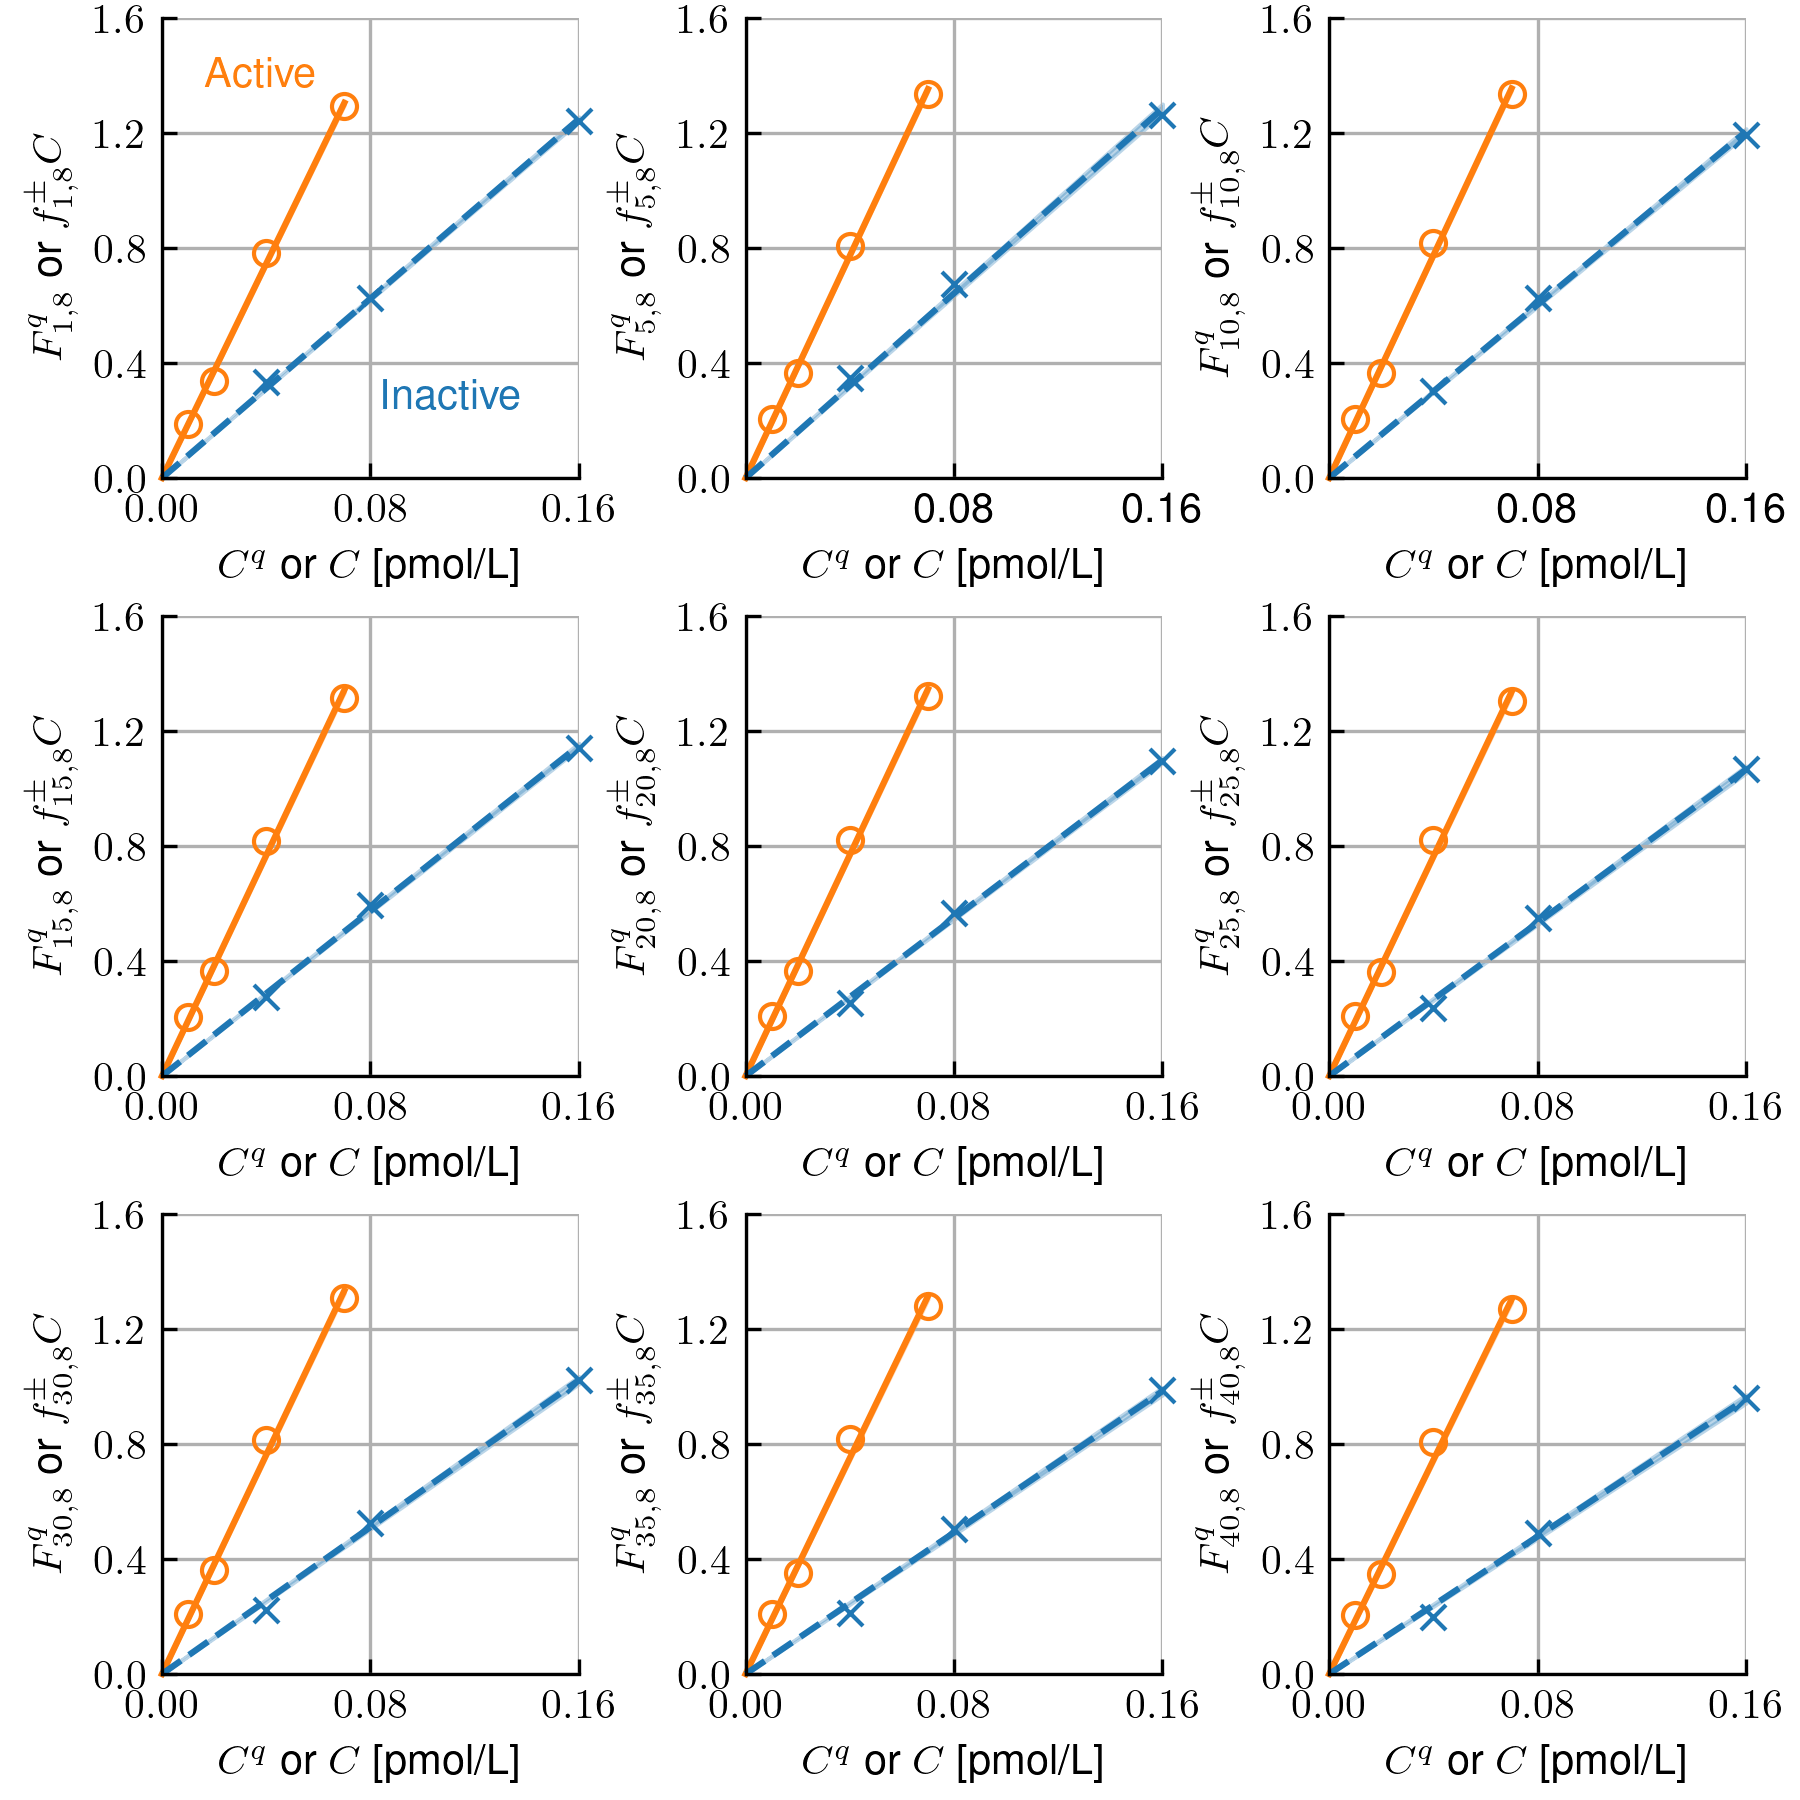
\includegraphics{si-figs/FigS8.png}
                    \caption{
                        As Figure~\ref{fig:S1} with well $w=8$ (or A8).
                    }
                \end{figure}
                \clearpage
    \begin{table}
        \caption{Molar Fluorescence Parameters for Well A8 ($w=8$)}
        \centering
        \begin{tabular}{c|ll|ll}
            Cycle & \multicolumn{2}{c|}{Inactive} & \multicolumn{2}{c}{Active} \\
            \hline
            $i$ & $f_{i,8}^{-}$ & $\sigma_{i,8}^{-}$ &  $f_{i,8}^{+}$ & $\sigma_{i,8}^{+}$ \\
            \hline
    1 & 7.80 & 0.015 & 18.64 & 0.030 \\
2 & 7.92 & 0.031 & 18.84 & 0.023 \\
3 & 8.08 & 0.034 & 19.11 & 0.026 \\
4 & 8.09 & 0.035 & 19.25 & 0.026 \\
5 & 8.03 & 0.034 & 19.32 & 0.026 \\
6 & 7.92 & 0.032 & 19.38 & 0.027 \\
7 & 7.82 & 0.029 & 19.38 & 0.028 \\
8 & 7.72 & 0.025 & 19.36 & 0.030 \\
9 & 7.63 & 0.022 & 19.29 & 0.028 \\
10 & 7.53 & 0.020 & 19.36 & 0.030 \\
11 & 7.43 & 0.019 & 19.32 & 0.030 \\
12 & 7.39 & 0.018 & 19.26 & 0.031 \\
13 & 7.31 & 0.017 & 19.23 & 0.032 \\
14 & 7.24 & 0.017 & 19.19 & 0.035 \\
15 & 7.18 & 0.018 & 19.18 & 0.036 \\
16 & 7.15 & 0.016 & 19.22 & 0.034 \\
17 & 7.08 & 0.017 & 19.18 & 0.035 \\
18 & 7.00 & 0.018 & 19.17 & 0.038 \\
19 & 6.98 & 0.017 & 19.24 & 0.036 \\
20 & 6.86 & 0.019 & 19.22 & 0.036 \\
21 & 6.82 & 0.020 & 19.15 & 0.038 \\
22 & 6.77 & 0.020 & 19.12 & 0.039 \\
23 & 6.71 & 0.021 & 19.13 & 0.039 \\
24 & 6.66 & 0.022 & 19.09 & 0.042 \\
25 & 6.66 & 0.025 & 19.08 & 0.041 \\
26 & 6.59 & 0.029 & 19.07 & 0.042 \\
27 & 6.51 & 0.026 & 19.06 & 0.040 \\
28 & 6.47 & 0.026 & 19.04 & 0.042 \\
29 & 6.48 & 0.029 & 19.17 & 0.037 \\
30 & 6.39 & 0.026 & 19.05 & 0.038 \\
31 & 6.37 & 0.029 & 19.19 & 0.035 \\
32 & 6.28 & 0.027 & 18.92 & 0.045 \\
33 & 6.25 & 0.027 & 18.84 & 0.045 \\
34 & 6.20 & 0.029 & 18.78 & 0.045 \\
35 & 6.15 & 0.027 & 18.77 & 0.048 \\
36 & 6.13 & 0.027 & 18.74 & 0.049 \\
37 & 6.10 & 0.027 & 18.72 & 0.047 \\
38 & 6.05 & 0.028 & 18.69 & 0.048 \\
39 & 6.02 & 0.029 & 18.67 & 0.048 \\
40 & 5.98 & 0.030 & 18.60 & 0.045 \\
41 & 5.97 & 0.029 & 18.49 & 0.046 \\
42 & 5.96 & 0.030 & 18.49 & 0.046 \\
43 & 5.95 & 0.031 & 18.53 & 0.046 \\
44 & 5.93 & 0.032 & 18.49 & 0.046 \\
45 & 5.91 & 0.033 & 18.47 & 0.047 \\
               \hline
        \end{tabular}
    \end{table}
    \clearpage

                \begin{figure}
                    \centering
                    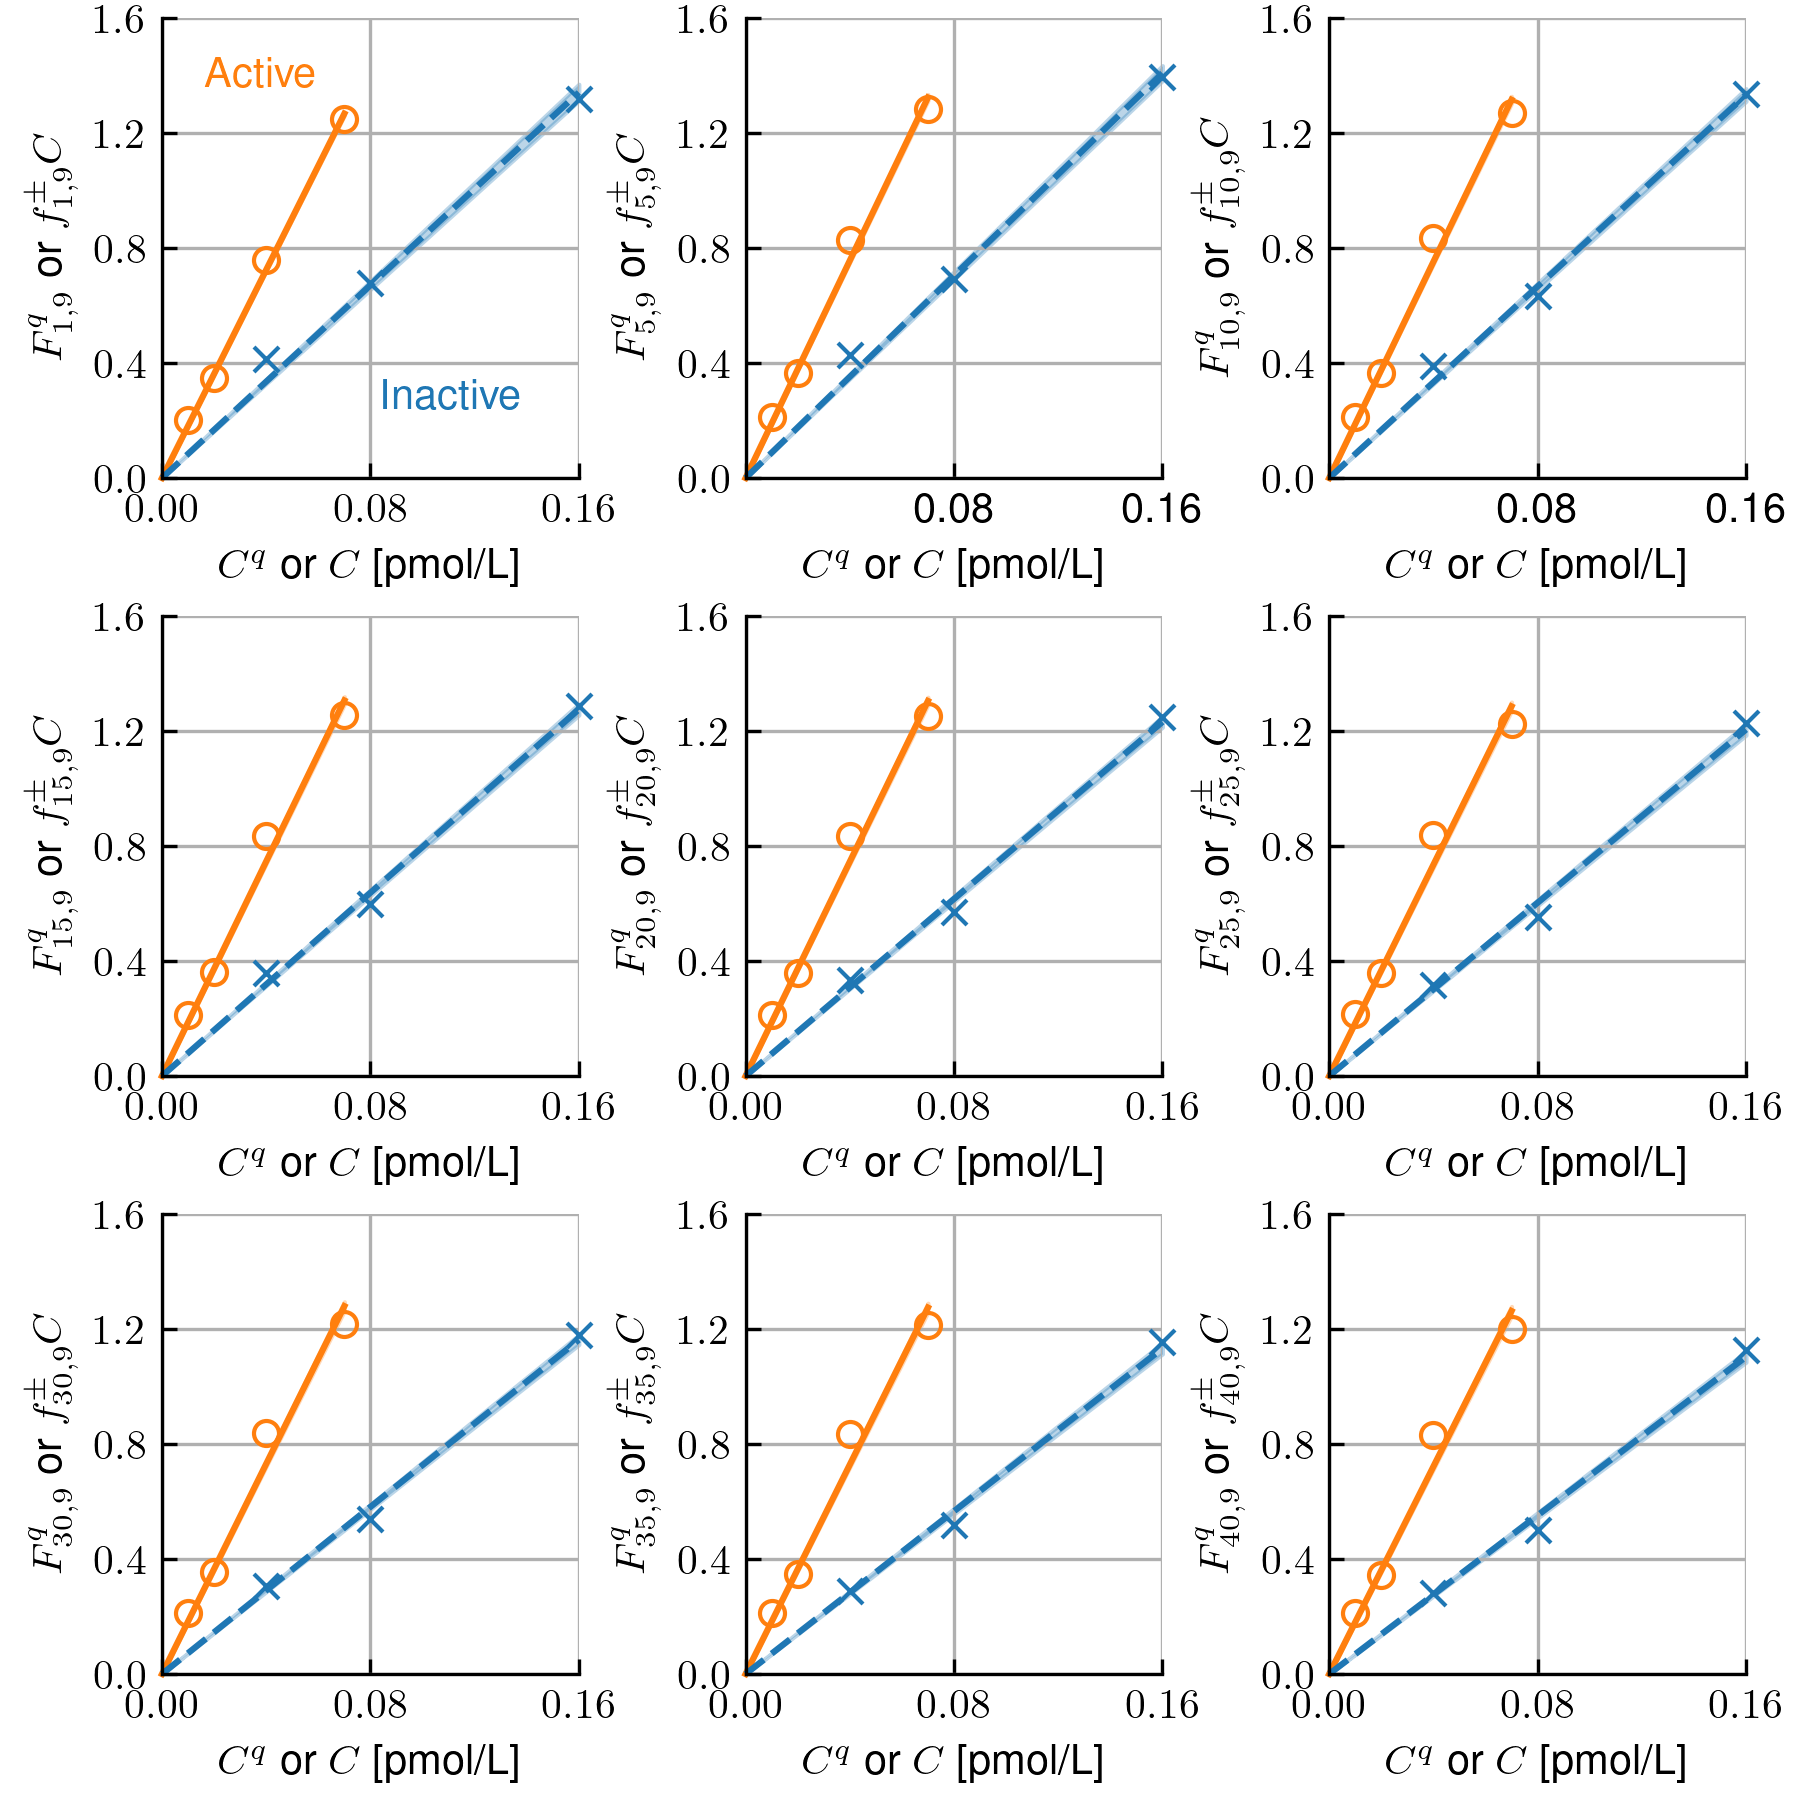
\includegraphics{si-figs/FigS9.png}
                    \caption{
                        As Figure~\ref{fig:S1} with well $w=9$ (or A9).
                    }
                \end{figure}
                \clearpage
    \begin{table}
        \caption{Molar Fluorescence Parameters for Well A9 ($w=9$)}
        \centering
        \begin{tabular}{c|ll|ll}
            Cycle & \multicolumn{2}{c|}{Inactive} & \multicolumn{2}{c}{Active} \\
            \hline
            $i$ & $f_{i,9}^{-}$ & $\sigma_{i,9}^{-}$ &  $f_{i,9}^{+}$ & $\sigma_{i,9}^{+}$ \\
            \hline
    1 & 8.38 & 0.059 & 18.10 & 0.027 \\
2 & 8.64 & 0.054 & 18.39 & 0.041 \\
3 & 8.83 & 0.054 & 18.69 & 0.045 \\
4 & 8.87 & 0.055 & 18.85 & 0.048 \\
5 & 8.80 & 0.054 & 18.91 & 0.051 \\
6 & 8.72 & 0.052 & 18.90 & 0.053 \\
7 & 8.63 & 0.049 & 18.86 & 0.055 \\
8 & 8.50 & 0.048 & 18.84 & 0.056 \\
9 & 8.42 & 0.047 & 18.82 & 0.057 \\
10 & 8.33 & 0.046 & 18.80 & 0.057 \\
11 & 8.24 & 0.044 & 18.75 & 0.059 \\
12 & 8.16 & 0.043 & 18.74 & 0.059 \\
13 & 8.10 & 0.042 & 18.69 & 0.060 \\
14 & 8.01 & 0.040 & 18.67 & 0.061 \\
15 & 7.97 & 0.040 & 18.66 & 0.062 \\
16 & 7.93 & 0.041 & 18.61 & 0.063 \\
17 & 7.85 & 0.038 & 18.63 & 0.063 \\
18 & 7.80 & 0.039 & 18.62 & 0.063 \\
19 & 7.74 & 0.039 & 18.62 & 0.063 \\
20 & 7.70 & 0.038 & 18.63 & 0.062 \\
21 & 7.67 & 0.038 & 18.51 & 0.066 \\
22 & 7.60 & 0.037 & 18.49 & 0.067 \\
23 & 7.58 & 0.038 & 18.43 & 0.069 \\
24 & 7.54 & 0.039 & 18.38 & 0.071 \\
25 & 7.53 & 0.040 & 18.37 & 0.072 \\
26 & 7.43 & 0.037 & 18.35 & 0.072 \\
27 & 7.39 & 0.036 & 18.32 & 0.073 \\
28 & 7.35 & 0.038 & 18.33 & 0.072 \\
29 & 7.32 & 0.034 & 18.31 & 0.074 \\
30 & 7.27 & 0.035 & 18.28 & 0.074 \\
31 & 7.20 & 0.037 & 18.31 & 0.074 \\
32 & 7.18 & 0.039 & 18.28 & 0.074 \\
33 & 7.15 & 0.040 & 18.25 & 0.073 \\
34 & 7.12 & 0.041 & 18.25 & 0.073 \\
35 & 7.08 & 0.039 & 18.21 & 0.074 \\
36 & 7.06 & 0.039 & 18.16 & 0.075 \\
37 & 6.97 & 0.038 & 18.14 & 0.075 \\
38 & 6.96 & 0.041 & 18.09 & 0.077 \\
39 & 6.93 & 0.040 & 18.06 & 0.076 \\
40 & 6.89 & 0.039 & 18.04 & 0.077 \\
41 & 6.91 & 0.041 & 17.87 & 0.082 \\
42 & 6.89 & 0.041 & 17.92 & 0.080 \\
43 & 6.86 & 0.040 & 17.90 & 0.082 \\
44 & 6.87 & 0.039 & 17.76 & 0.071 \\
45 & 6.82 & 0.038 & 17.76 & 0.073 \\
               \hline
        \end{tabular}
    \end{table}
    \clearpage

                \begin{figure}
                    \centering
                    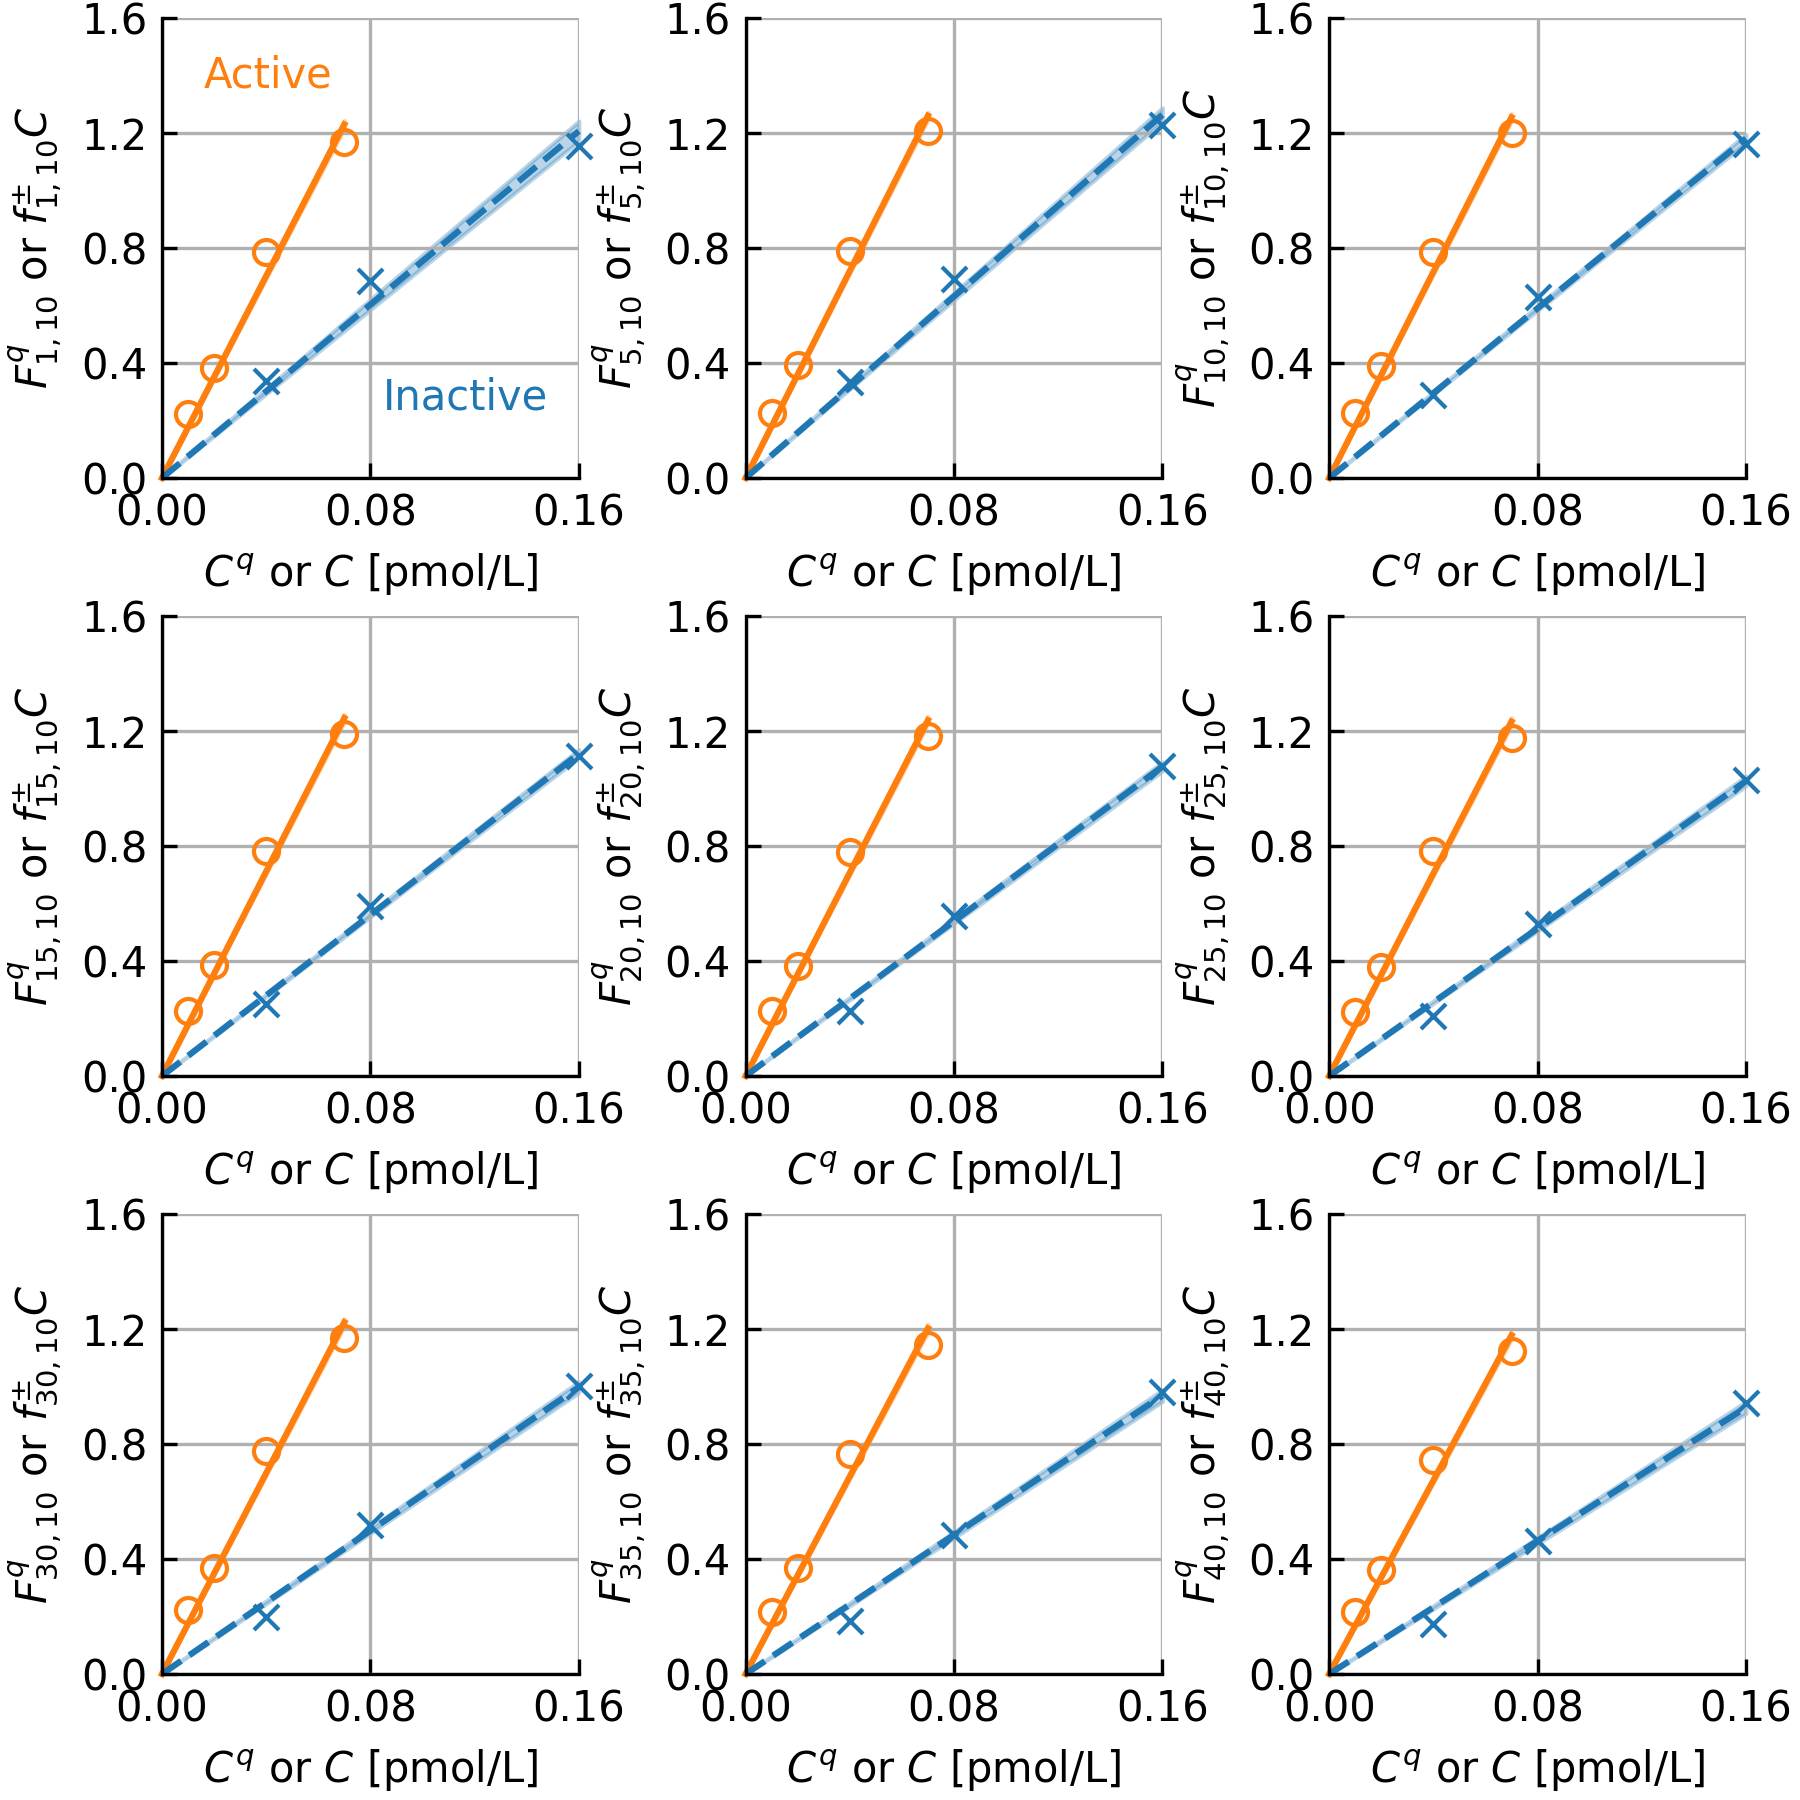
\includegraphics{si-figs/FigS10.png}
                    \caption{
                        As Figure~\ref{fig:S1} with well $w=10$ (or A10).
                    }
                \end{figure}
                \clearpage
    \begin{table}
        \caption{Molar Fluorescence Parameters for Well A10 ($w=10$)}
        \centering
        \begin{tabular}{c|ll|ll}
            Cycle & \multicolumn{2}{c|}{Inactive} & \multicolumn{2}{c}{Active} \\
            \hline
            $i$ & $f_{i,10}^{-}$ & $\sigma_{i,10}^{-}$ &  $f_{i,10}^{+}$ & $\sigma_{i,10}^{+}$ \\
            \hline
    1 & 7.54 & 0.073 & 17.57 & 0.067 \\
2 & 7.82 & 0.066 & 17.55 & 0.061 \\
3 & 7.99 & 0.064 & 17.83 & 0.062 \\
4 & 7.97 & 0.058 & 17.94 & 0.061 \\
5 & 7.89 & 0.051 & 18.00 & 0.060 \\
6 & 7.79 & 0.045 & 18.00 & 0.060 \\
7 & 7.68 & 0.041 & 17.98 & 0.061 \\
8 & 7.57 & 0.037 & 17.94 & 0.061 \\
9 & 7.48 & 0.034 & 17.94 & 0.061 \\
10 & 7.38 & 0.031 & 17.92 & 0.061 \\
11 & 7.31 & 0.030 & 17.88 & 0.062 \\
12 & 7.24 & 0.028 & 17.86 & 0.062 \\
13 & 7.18 & 0.028 & 17.85 & 0.062 \\
14 & 7.10 & 0.028 & 17.82 & 0.062 \\
15 & 7.01 & 0.029 & 17.79 & 0.061 \\
16 & 6.95 & 0.030 & 17.79 & 0.062 \\
17 & 6.94 & 0.030 & 17.76 & 0.062 \\
18 & 6.87 & 0.030 & 17.70 & 0.062 \\
19 & 6.78 & 0.032 & 17.73 & 0.062 \\
20 & 6.73 & 0.032 & 17.68 & 0.062 \\
21 & 6.72 & 0.039 & 17.68 & 0.061 \\
22 & 6.60 & 0.033 & 17.76 & 0.058 \\
23 & 6.54 & 0.034 & 17.63 & 0.061 \\
24 & 6.48 & 0.035 & 17.62 & 0.061 \\
25 & 6.41 & 0.035 & 17.61 & 0.064 \\
26 & 6.36 & 0.035 & 17.57 & 0.062 \\
27 & 6.32 & 0.034 & 17.55 & 0.062 \\
28 & 6.29 & 0.033 & 17.51 & 0.063 \\
29 & 6.26 & 0.036 & 17.46 & 0.062 \\
30 & 6.24 & 0.040 & 17.48 & 0.062 \\
31 & 6.20 & 0.038 & 17.31 & 0.066 \\
32 & 6.16 & 0.039 & 17.25 & 0.066 \\
33 & 6.11 & 0.040 & 17.23 & 0.065 \\
34 & 6.11 & 0.041 & 17.20 & 0.064 \\
35 & 6.05 & 0.042 & 17.18 & 0.064 \\
36 & 6.02 & 0.042 & 17.13 & 0.063 \\
37 & 5.90 & 0.040 & 17.12 & 0.064 \\
38 & 5.86 & 0.041 & 16.94 & 0.054 \\
39 & 5.82 & 0.042 & 16.97 & 0.056 \\
40 & 5.79 & 0.043 & 16.83 & 0.060 \\
41 & 5.71 & 0.042 & 16.77 & 0.062 \\
42 & 5.67 & 0.043 & 16.78 & 0.062 \\
43 & 5.63 & 0.044 & 16.78 & 0.062 \\
44 & 5.60 & 0.045 & 16.76 & 0.062 \\
45 & 5.57 & 0.046 & 16.75 & 0.062 \\
               \hline
        \end{tabular}
    \end{table}
    \clearpage

                \begin{figure}
                    \centering
                    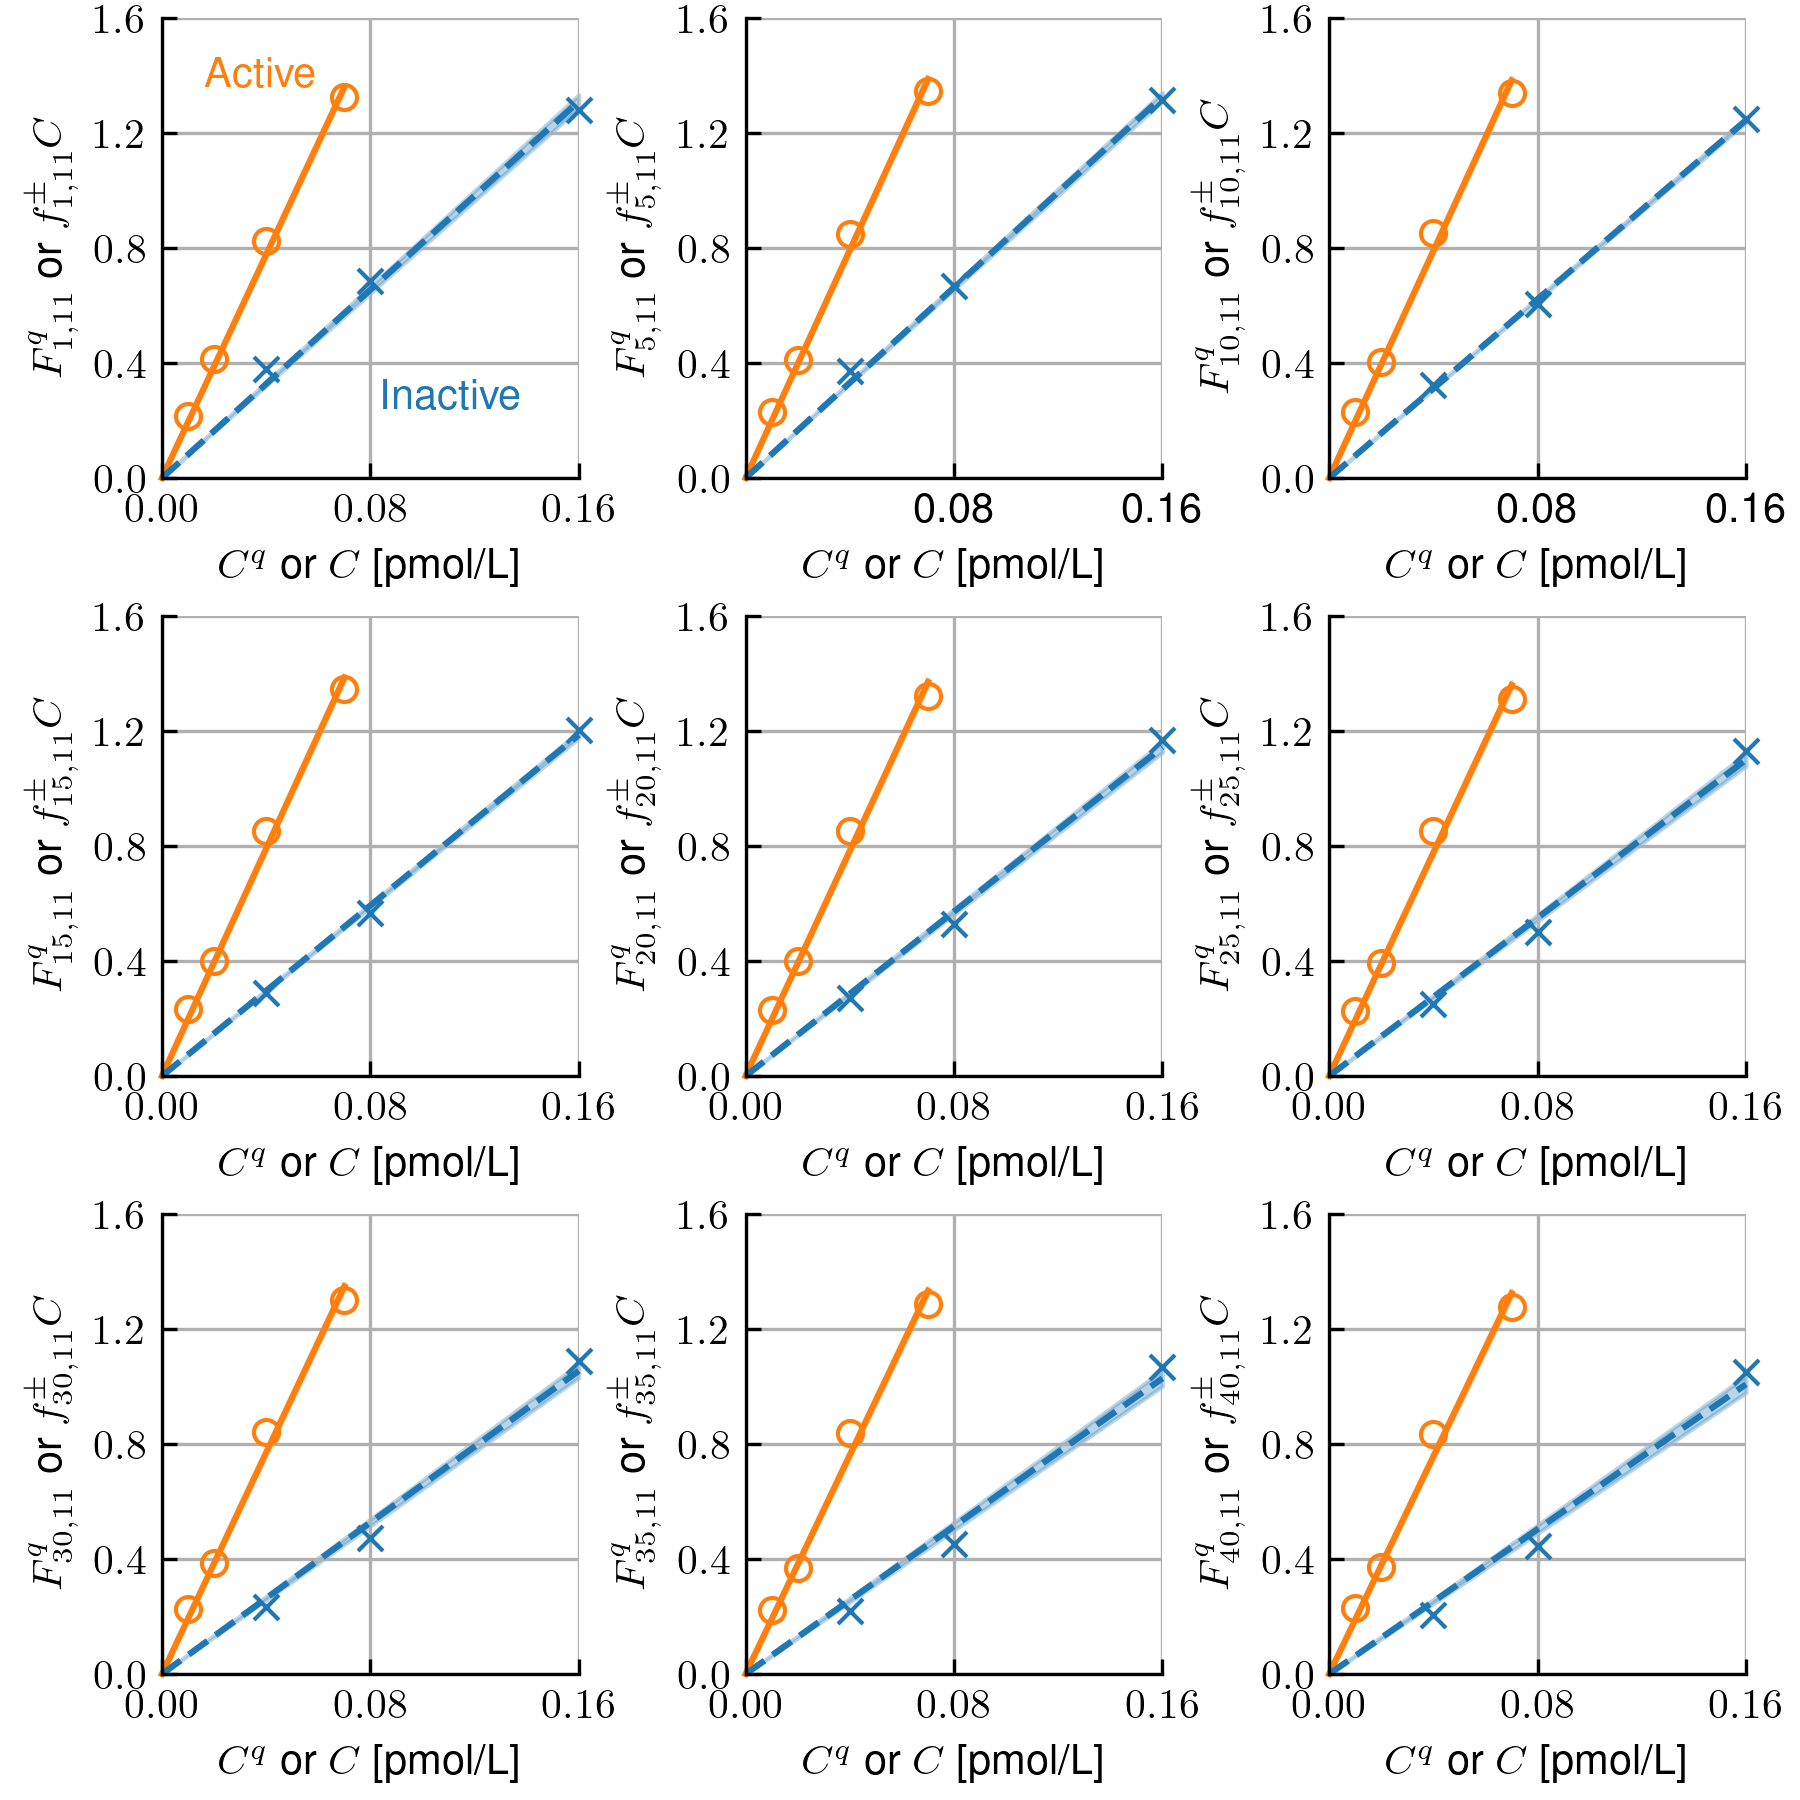
\includegraphics{si-figs/FigS11.png}
                    \caption{
                        As Figure~\ref{fig:S1} with well $w=11$ (or A11).
                    }
                \end{figure}
                \clearpage
    \begin{table}
        \caption{Molar Fluorescence Parameters for Well A11 ($w=11$)}
        \centering
        \begin{tabular}{c|ll|ll}
            Cycle & \multicolumn{2}{c|}{Inactive} & \multicolumn{2}{c}{Active} \\
            \hline
            $i$ & $f_{i,11}^{-}$ & $\sigma_{i,11}^{-}$ &  $f_{i,11}^{+}$ & $\sigma_{i,11}^{+}$ \\
            \hline
    1 & 8.19 & 0.048 & 19.43 & 0.038 \\
2 & 8.34 & 0.043 & 19.38 & 0.036 \\
3 & 8.42 & 0.041 & 19.61 & 0.040 \\
4 & 8.39 & 0.036 & 19.78 & 0.044 \\
5 & 8.29 & 0.031 & 19.82 & 0.046 \\
6 & 8.17 & 0.025 & 19.81 & 0.046 \\
7 & 8.07 & 0.021 & 19.81 & 0.048 \\
8 & 7.97 & 0.018 & 19.78 & 0.048 \\
9 & 7.88 & 0.016 & 19.75 & 0.049 \\
10 & 7.78 & 0.016 & 19.75 & 0.049 \\
11 & 7.70 & 0.016 & 19.78 & 0.048 \\
12 & 7.63 & 0.019 & 19.73 & 0.050 \\
13 & 7.56 & 0.021 & 19.68 & 0.050 \\
14 & 7.49 & 0.023 & 19.65 & 0.051 \\
15 & 7.42 & 0.023 & 19.79 & 0.046 \\
16 & 7.34 & 0.024 & 19.68 & 0.050 \\
17 & 7.35 & 0.033 & 19.65 & 0.051 \\
18 & 7.26 & 0.033 & 19.77 & 0.047 \\
19 & 7.20 & 0.033 & 19.62 & 0.052 \\
20 & 7.15 & 0.037 & 19.58 & 0.053 \\
21 & 7.09 & 0.039 & 19.54 & 0.055 \\
22 & 7.02 & 0.039 & 19.48 & 0.056 \\
23 & 6.94 & 0.039 & 19.53 & 0.058 \\
24 & 6.89 & 0.044 & 19.49 & 0.057 \\
25 & 6.87 & 0.045 & 19.43 & 0.056 \\
26 & 6.78 & 0.043 & 19.50 & 0.061 \\
27 & 6.70 & 0.043 & 19.39 & 0.051 \\
28 & 6.67 & 0.043 & 19.40 & 0.050 \\
29 & 6.61 & 0.049 & 19.36 & 0.051 \\
30 & 6.59 & 0.050 & 19.26 & 0.053 \\
31 & 6.58 & 0.051 & 19.12 & 0.056 \\
32 & 6.53 & 0.053 & 19.12 & 0.056 \\
33 & 6.50 & 0.056 & 19.11 & 0.055 \\
34 & 6.50 & 0.060 & 19.12 & 0.055 \\
35 & 6.43 & 0.058 & 19.04 & 0.056 \\
36 & 6.39 & 0.057 & 19.08 & 0.059 \\
37 & 6.35 & 0.058 & 19.03 & 0.057 \\
38 & 6.33 & 0.058 & 19.07 & 0.054 \\
39 & 6.30 & 0.059 & 18.97 & 0.057 \\
40 & 6.30 & 0.061 & 18.92 & 0.057 \\
41 & 6.25 & 0.060 & 18.89 & 0.058 \\
42 & 6.22 & 0.060 & 18.74 & 0.061 \\
43 & 6.17 & 0.061 & 18.81 & 0.060 \\
44 & 6.17 & 0.065 & 18.81 & 0.060 \\
45 & 6.15 & 0.065 & 18.78 & 0.062 \\
               \hline
        \end{tabular}
    \end{table}
    \clearpage

                \begin{figure}
                    \centering
                    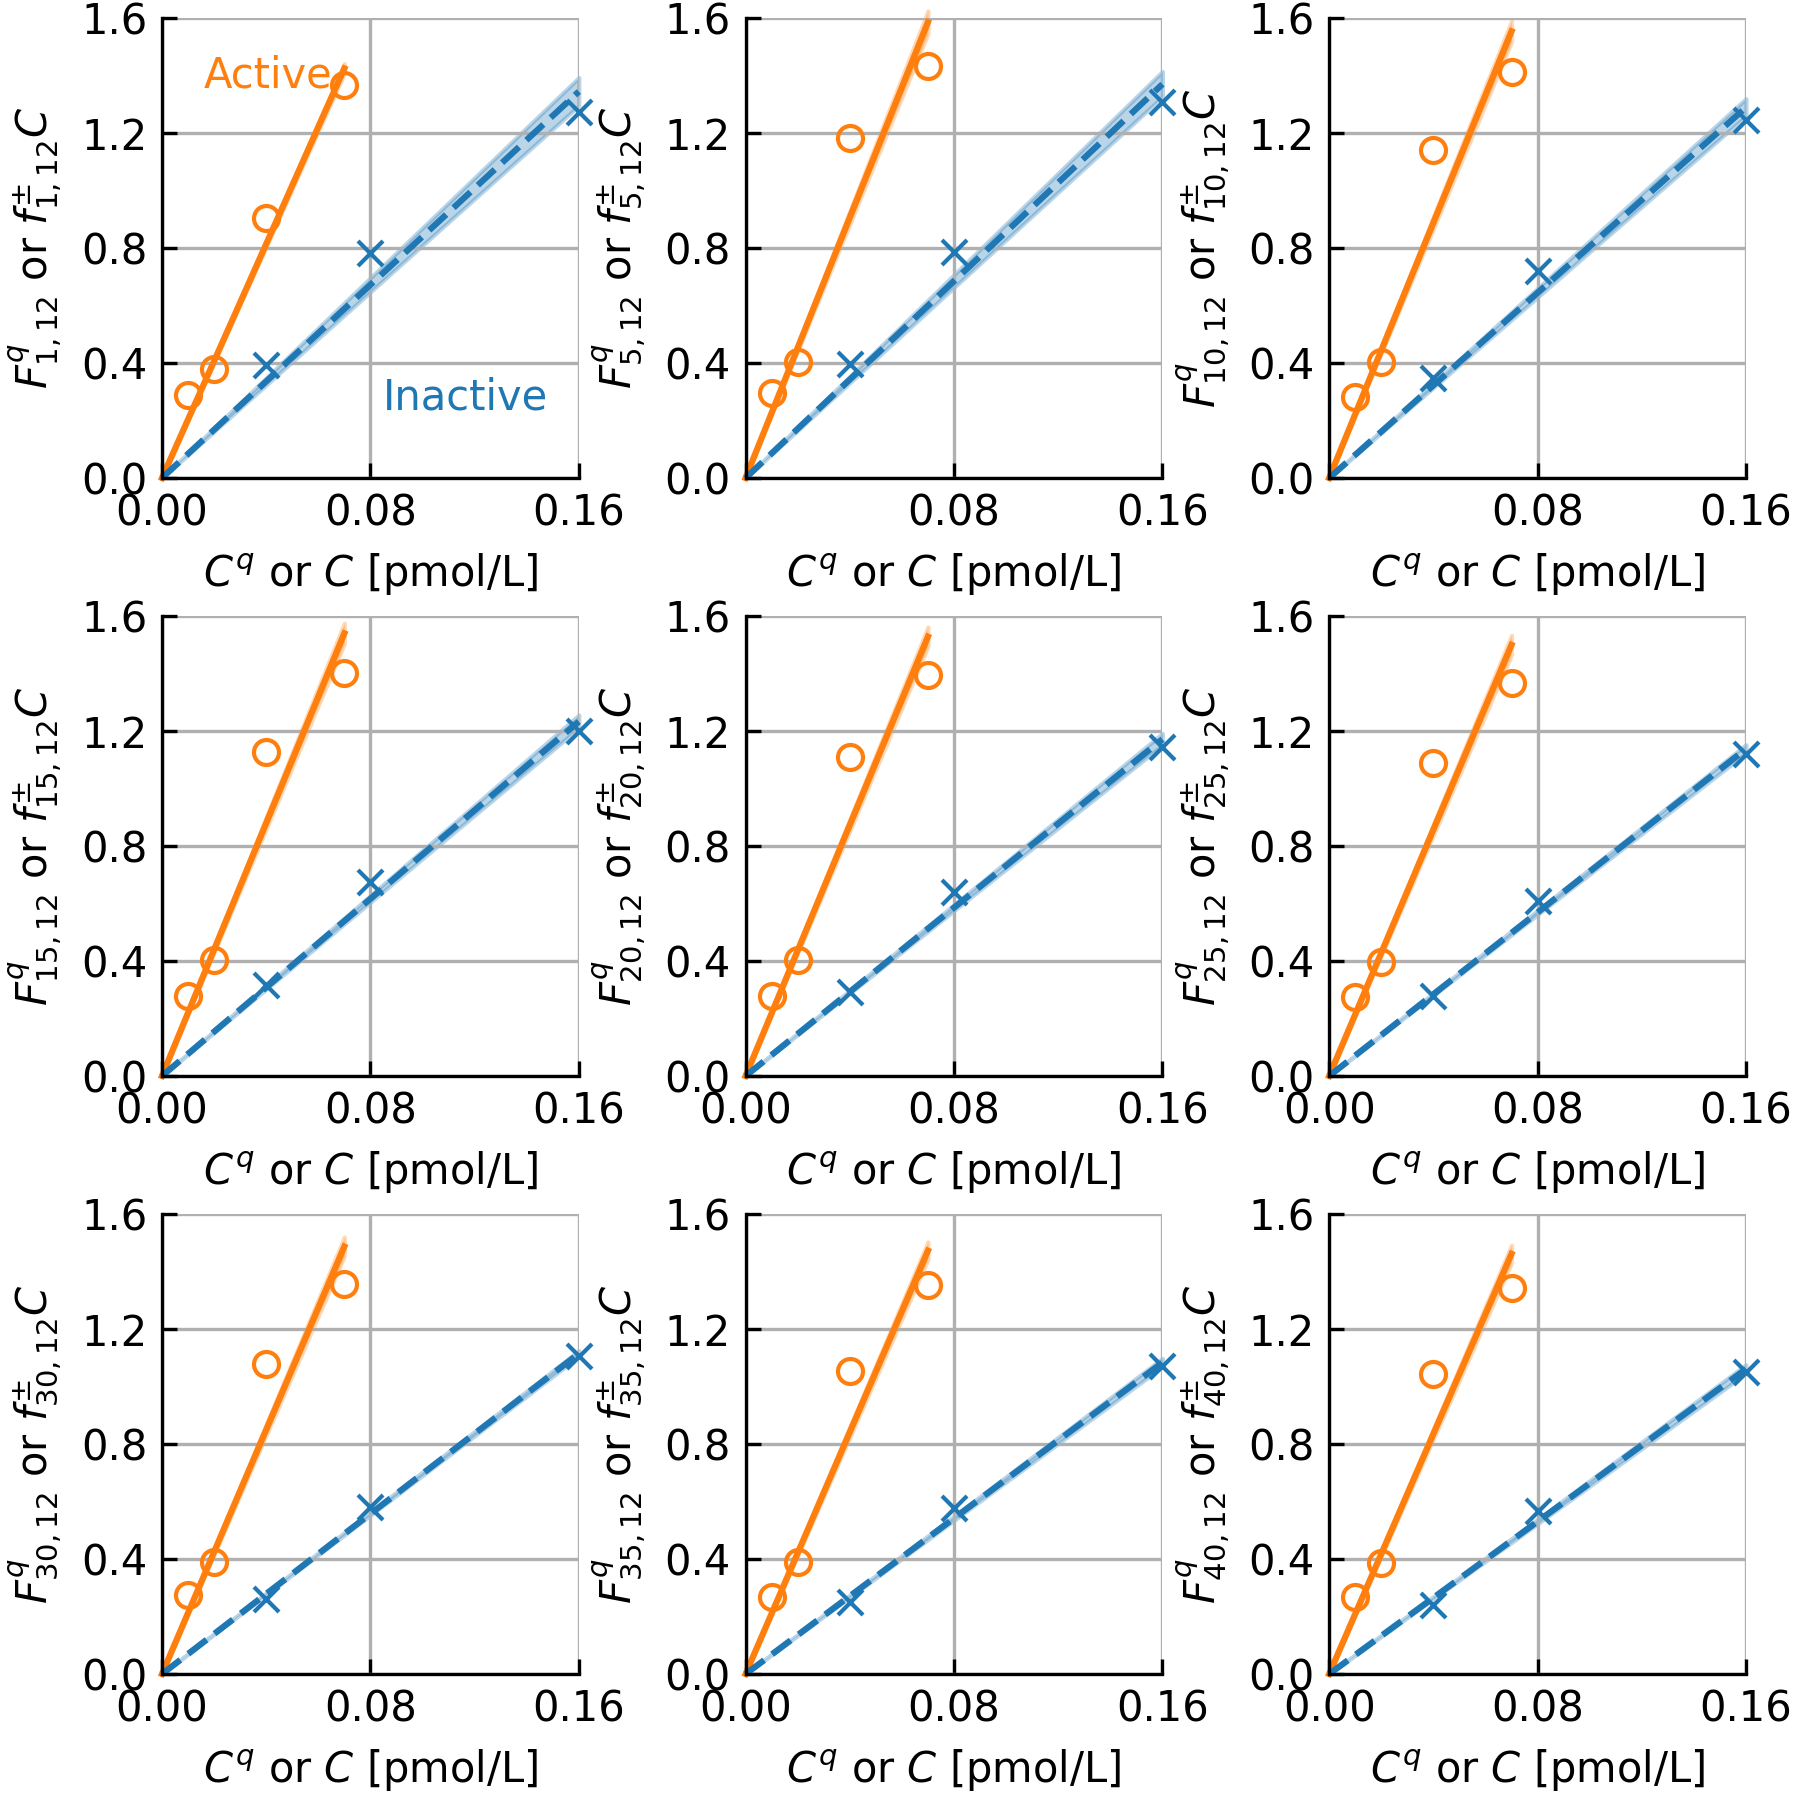
\includegraphics{si-figs/FigS12.png}
                    \caption{
                        As Figure~\ref{fig:S1} with well $w=12$ (or A12).
                    }
                \end{figure}
                \clearpage
    \begin{table}
        \caption{Molar Fluorescence Parameters for Well A12 ($w=12$)}
        \centering
        \begin{tabular}{c|ll|ll}
            Cycle & \multicolumn{2}{c|}{Inactive} & \multicolumn{2}{c}{Active} \\
            \hline
            $i$ & $f_{i,12}^{-}$ & $\sigma_{i,12}^{-}$ &  $f_{i,12}^{+}$ & $\sigma_{i,12}^{+}$ \\
            \hline
    1 & 8.4 & 0.10 & 20.35 & 0.081 \\
2 & 8.6 & 0.10 & 21.0 & 0.10 \\
3 & 8.7 & 0.10 & 22.2 & 0.17 \\
4 & 8.64 & 0.100 & 22.5 & 0.19 \\
5 & 8.56 & 0.092 & 22.6 & 0.19 \\
6 & 8.44 & 0.086 & 22.5 & 0.18 \\
7 & 8.34 & 0.079 & 22.4 & 0.18 \\
8 & 8.24 & 0.073 & 22.3 & 0.17 \\
9 & 8.15 & 0.069 & 22.3 & 0.17 \\
10 & 8.06 & 0.064 & 22.2 & 0.17 \\
11 & 7.98 & 0.060 & 22.1 & 0.17 \\
12 & 7.90 & 0.057 & 22.1 & 0.17 \\
13 & 7.83 & 0.053 & 22.1 & 0.17 \\
14 & 7.78 & 0.050 & 22.0 & 0.17 \\
15 & 7.70 & 0.048 & 22.0 & 0.17 \\
16 & 7.64 & 0.046 & 22.0 & 0.17 \\
17 & 7.54 & 0.047 & 22.0 & 0.17 \\
18 & 7.48 & 0.044 & 22.0 & 0.16 \\
19 & 7.44 & 0.047 & 21.9 & 0.16 \\
20 & 7.32 & 0.042 & 21.8 & 0.16 \\
21 & 7.30 & 0.042 & 21.8 & 0.16 \\
22 & 7.23 & 0.037 & 21.8 & 0.16 \\
23 & 7.21 & 0.034 & 21.7 & 0.16 \\
24 & 7.15 & 0.032 & 21.6 & 0.16 \\
25 & 7.11 & 0.031 & 21.4 & 0.16 \\
26 & 7.07 & 0.030 & 21.3 & 0.16 \\
27 & 7.07 & 0.027 & 21.3 & 0.16 \\
28 & 7.01 & 0.027 & 21.3 & 0.15 \\
29 & 7.01 & 0.024 & 21.2 & 0.15 \\
30 & 6.97 & 0.021 & 21.2 & 0.16 \\
31 & 6.95 & 0.029 & 21.2 & 0.15 \\
32 & 6.89 & 0.030 & 21.1 & 0.15 \\
33 & 6.85 & 0.030 & 21.1 & 0.15 \\
34 & 6.81 & 0.029 & 21.0 & 0.14 \\
35 & 6.77 & 0.030 & 21.0 & 0.15 \\
36 & 6.73 & 0.033 & 21.0 & 0.15 \\
37 & 6.72 & 0.030 & 21.0 & 0.14 \\
38 & 6.70 & 0.031 & 21.0 & 0.14 \\
39 & 6.65 & 0.031 & 20.9 & 0.14 \\
40 & 6.63 & 0.032 & 20.9 & 0.14 \\
41 & 6.44 & 0.029 & 20.7 & 0.13 \\
42 & 6.43 & 0.034 & 20.5 & 0.14 \\
43 & 6.39 & 0.030 & 20.6 & 0.14 \\
44 & 6.36 & 0.029 & 20.6 & 0.14 \\
45 & 6.35 & 0.026 & 20.6 & 0.14 \\
               \hline
        \end{tabular}
    \end{table}
    \clearpage

                \begin{figure}
                    \centering
                    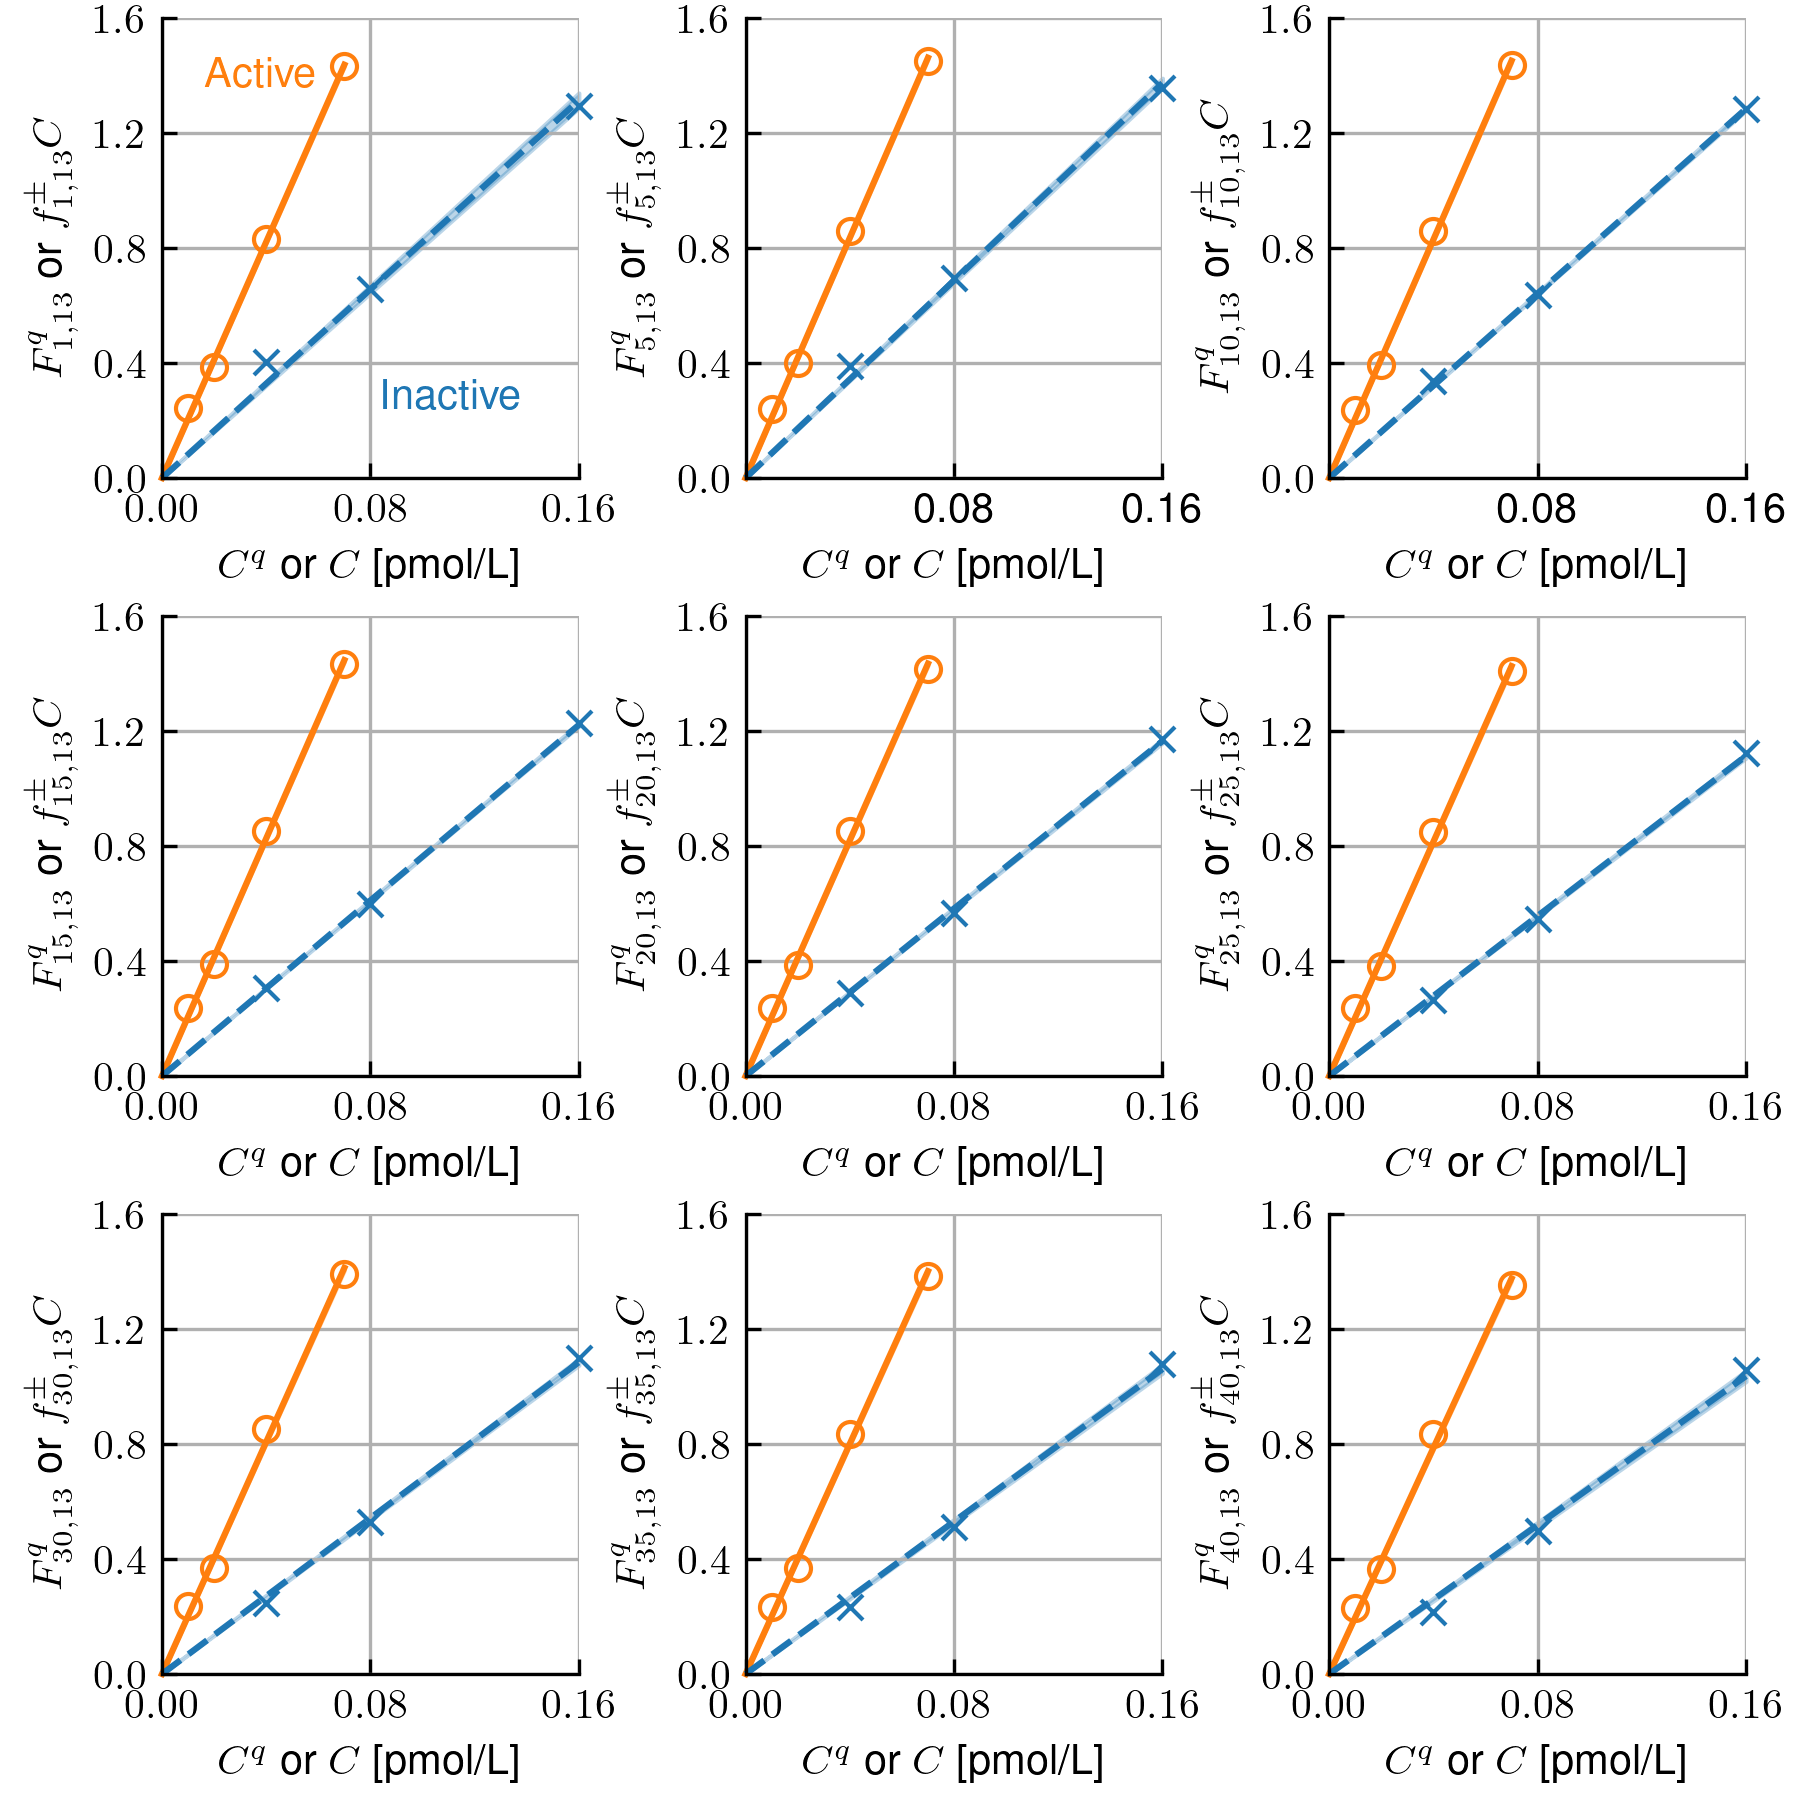
\includegraphics{si-figs/FigS13.png}
                    \caption{
                        As Figure~\ref{fig:S1} with well $w=13$ (or B1).
                    }
                \end{figure}
                \clearpage
    \begin{table}
        \caption{Molar Fluorescence Parameters for Well B1 ($w=13$)}
        \centering
        \begin{tabular}{c|ll|ll}
            Cycle & \multicolumn{2}{c|}{Inactive} & \multicolumn{2}{c}{Active} \\
            \hline
            $i$ & $f_{i,13}^{-}$ & $\sigma_{i,13}^{-}$ &  $f_{i,13}^{+}$ & $\sigma_{i,13}^{+}$ \\
            \hline
    1 & 8.21 & 0.054 & 20.53 & 0.026 \\
2 & 8.58 & 0.048 & 20.57 & 0.023 \\
3 & 8.75 & 0.046 & 20.78 & 0.025 \\
4 & 8.70 & 0.041 & 20.86 & 0.025 \\
5 & 8.58 & 0.036 & 20.88 & 0.026 \\
6 & 8.45 & 0.030 & 20.84 & 0.025 \\
7 & 8.33 & 0.024 & 20.77 & 0.028 \\
8 & 8.24 & 0.019 & 20.80 & 0.027 \\
9 & 8.12 & 0.015 & 20.75 & 0.027 \\
10 & 8.03 & 0.013 & 20.73 & 0.029 \\
11 & 7.93 & 0.010 & 20.65 & 0.029 \\
12 & 7.844 & 0.0098 & 20.68 & 0.027 \\
13 & 7.76 & 0.011 & 20.63 & 0.028 \\
14 & 7.695 & 0.0096 & 20.59 & 0.029 \\
15 & 7.63 & 0.010 & 20.66 & 0.028 \\
16 & 7.59 & 0.014 & 20.62 & 0.032 \\
17 & 7.51 & 0.015 & 20.67 & 0.033 \\
18 & 7.40 & 0.013 & 20.55 & 0.031 \\
19 & 7.36 & 0.014 & 20.51 & 0.031 \\
20 & 7.28 & 0.013 & 20.49 & 0.032 \\
21 & 7.24 & 0.015 & 20.47 & 0.032 \\
22 & 7.23 & 0.020 & 20.46 & 0.032 \\
23 & 7.16 & 0.026 & 20.45 & 0.031 \\
24 & 7.01 & 0.015 & 20.41 & 0.032 \\
25 & 6.96 & 0.015 & 20.37 & 0.033 \\
26 & 6.92 & 0.015 & 20.35 & 0.033 \\
27 & 6.88 & 0.018 & 20.36 & 0.033 \\
28 & 6.85 & 0.021 & 20.29 & 0.035 \\
29 & 6.82 & 0.021 & 20.22 & 0.037 \\
30 & 6.78 & 0.023 & 20.18 & 0.039 \\
31 & 6.75 & 0.024 & 20.15 & 0.038 \\
32 & 6.70 & 0.025 & 20.14 & 0.040 \\
33 & 6.68 & 0.027 & 20.03 & 0.035 \\
34 & 6.66 & 0.028 & 20.00 & 0.035 \\
35 & 6.63 & 0.030 & 20.01 & 0.035 \\
36 & 6.60 & 0.032 & 20.01 & 0.035 \\
37 & 6.57 & 0.034 & 19.68 & 0.037 \\
38 & 6.54 & 0.038 & 19.80 & 0.036 \\
39 & 6.51 & 0.039 & 19.73 & 0.038 \\
40 & 6.48 & 0.039 & 19.65 & 0.040 \\
41 & 6.44 & 0.044 & 19.66 & 0.039 \\
42 & 6.42 & 0.045 & 19.69 & 0.038 \\
43 & 6.44 & 0.049 & 19.68 & 0.039 \\
44 & 6.24 & 0.041 & 19.66 & 0.039 \\
45 & 6.18 & 0.040 & 19.63 & 0.037 \\
               \hline
        \end{tabular}
    \end{table}
    \clearpage

                \begin{figure}
                    \centering
                    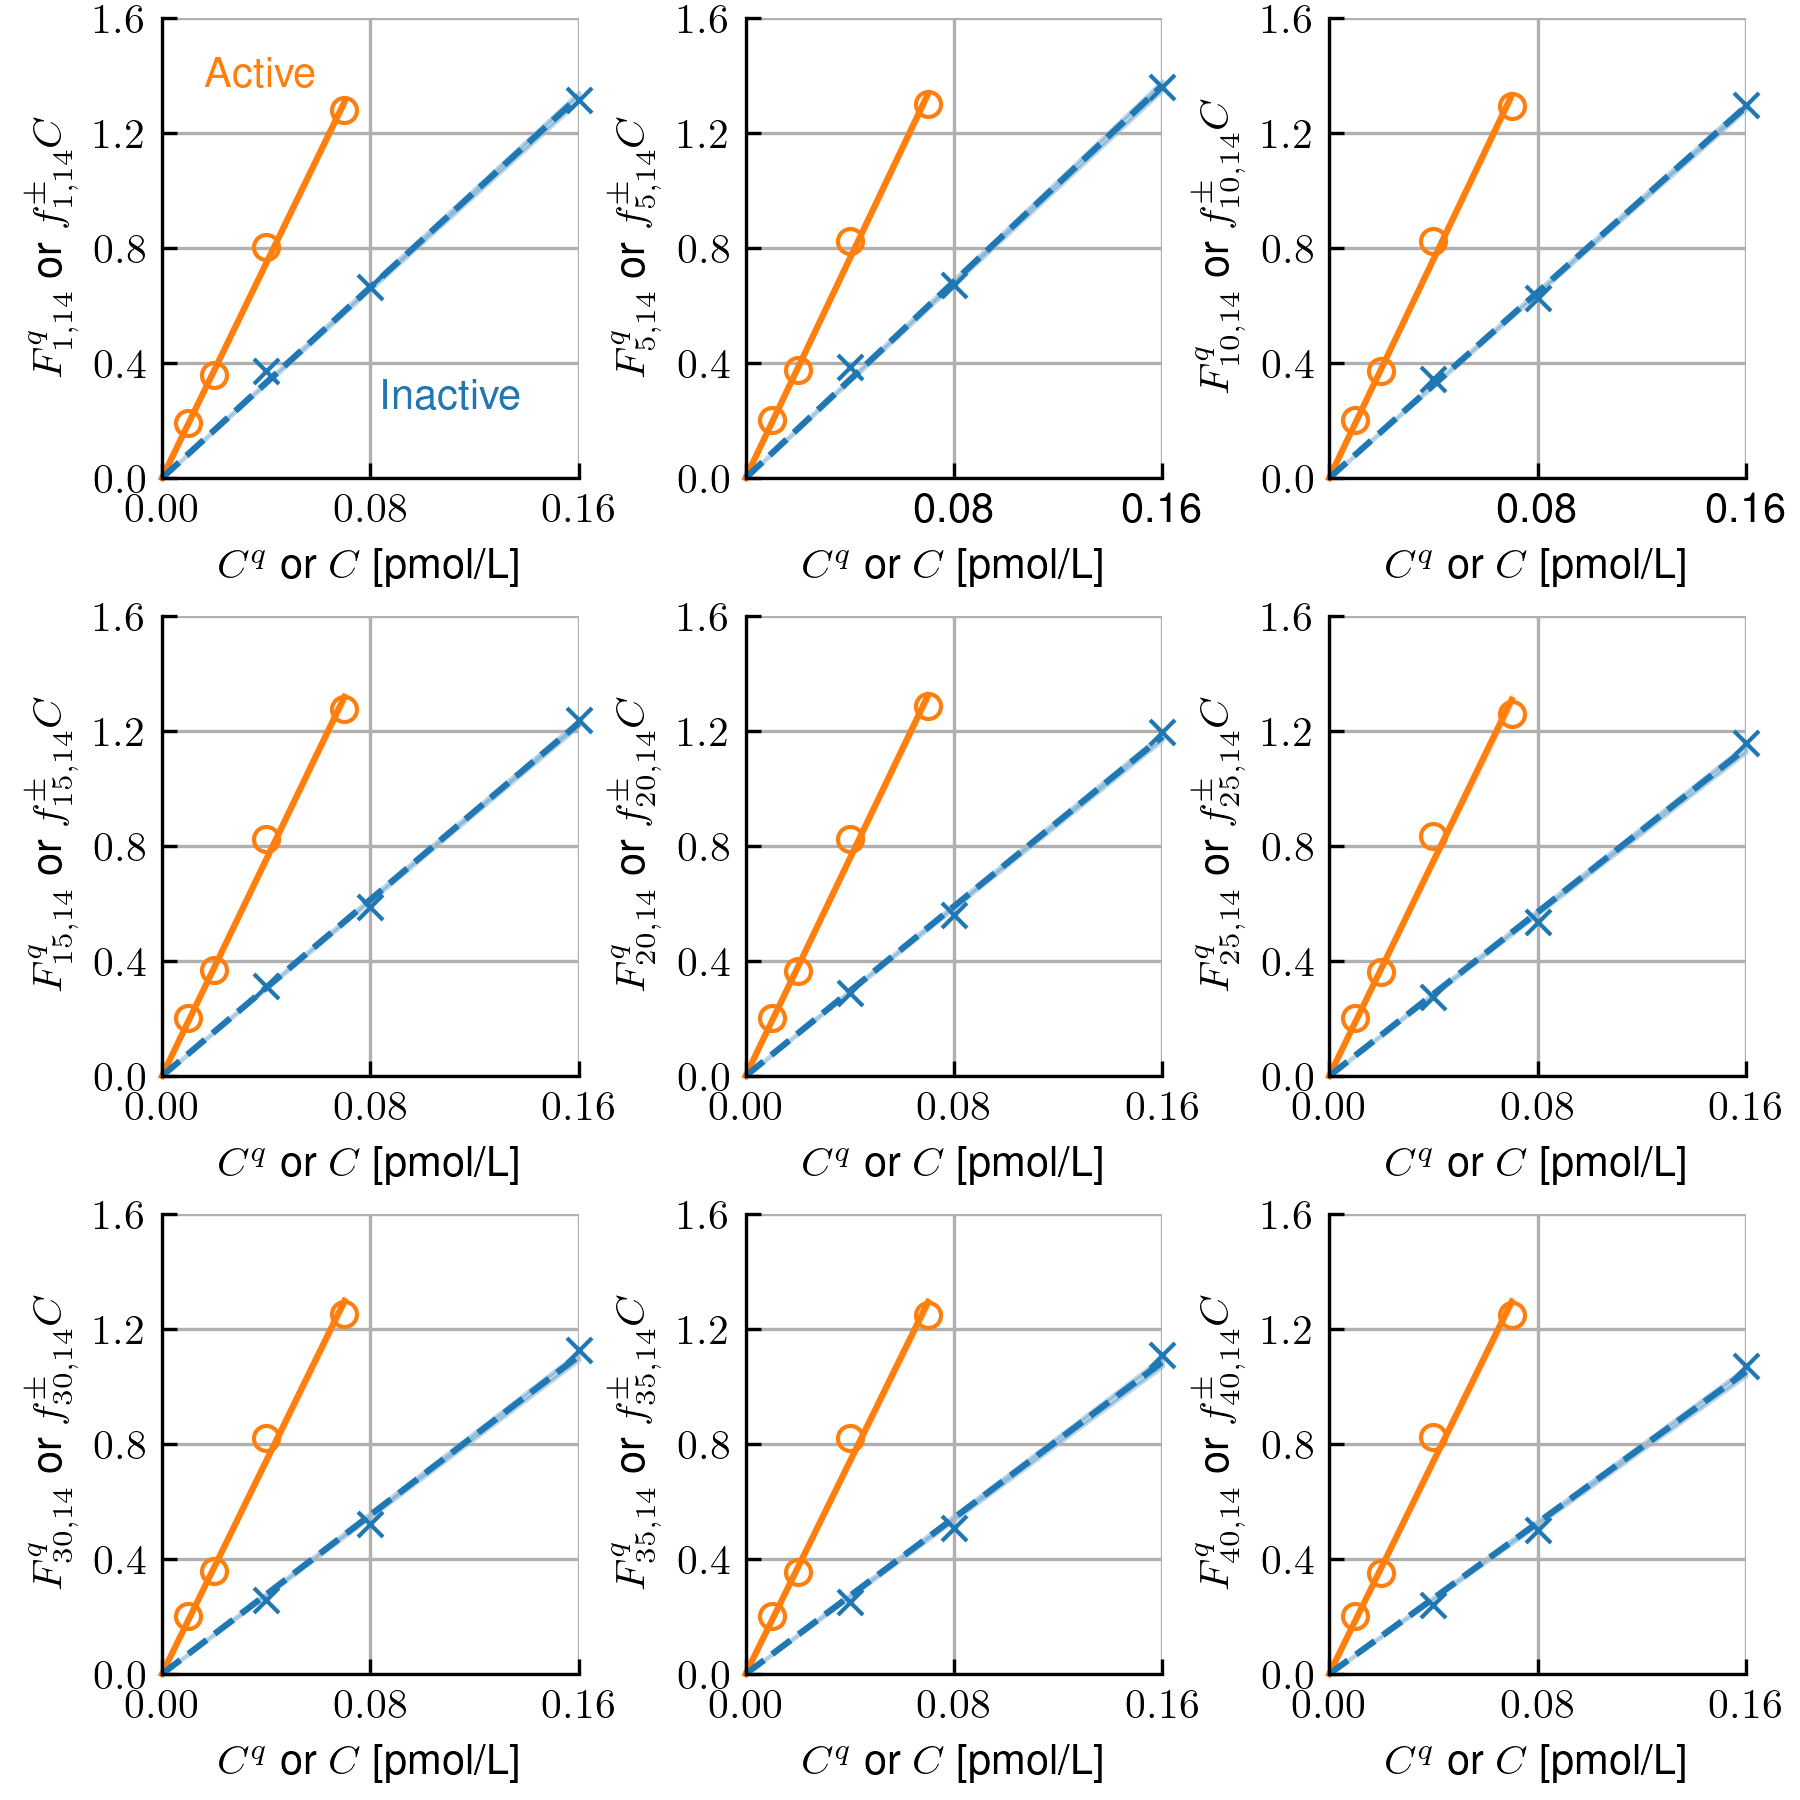
\includegraphics{si-figs/FigS14.png}
                    \caption{
                        As Figure~\ref{fig:S1} with well $w=14$ (or B2).
                    }
                \end{figure}
                \clearpage
    \begin{table}
        \caption{Molar Fluorescence Parameters for Well B2 ($w=14$)}
        \centering
        \begin{tabular}{c|ll|ll}
            Cycle & \multicolumn{2}{c|}{Inactive} & \multicolumn{2}{c}{Active} \\
            \hline
            $i$ & $f_{i,14}^{-}$ & $\sigma_{i,14}^{-}$ &  $f_{i,14}^{+}$ & $\sigma_{i,14}^{+}$ \\
            \hline
    1 & 8.29 & 0.030 & 18.68 & 0.038 \\
2 & 8.44 & 0.038 & 18.84 & 0.039 \\
3 & 8.60 & 0.037 & 19.03 & 0.039 \\
4 & 8.60 & 0.035 & 19.08 & 0.040 \\
5 & 8.53 & 0.033 & 19.08 & 0.041 \\
6 & 8.44 & 0.031 & 19.07 & 0.042 \\
7 & 8.36 & 0.028 & 19.08 & 0.042 \\
8 & 8.25 & 0.026 & 19.03 & 0.043 \\
9 & 8.15 & 0.023 & 18.98 & 0.045 \\
10 & 8.08 & 0.022 & 19.00 & 0.044 \\
11 & 8.00 & 0.020 & 18.99 & 0.045 \\
12 & 7.91 & 0.021 & 18.94 & 0.046 \\
13 & 7.82 & 0.020 & 18.95 & 0.046 \\
14 & 7.73 & 0.019 & 18.91 & 0.048 \\
15 & 7.67 & 0.020 & 18.83 & 0.049 \\
16 & 7.61 & 0.020 & 18.81 & 0.049 \\
17 & 7.54 & 0.020 & 18.84 & 0.049 \\
18 & 7.48 & 0.021 & 18.83 & 0.050 \\
19 & 7.42 & 0.022 & 18.82 & 0.049 \\
20 & 7.38 & 0.024 & 18.91 & 0.046 \\
21 & 7.32 & 0.027 & 18.70 & 0.052 \\
22 & 7.25 & 0.025 & 18.70 & 0.052 \\
23 & 7.23 & 0.025 & 18.66 & 0.053 \\
24 & 7.18 & 0.028 & 18.65 & 0.053 \\
25 & 7.12 & 0.027 & 18.69 & 0.059 \\
26 & 7.06 & 0.028 & 18.62 & 0.054 \\
27 & 7.05 & 0.032 & 18.75 & 0.053 \\
28 & 7.01 & 0.031 & 18.65 & 0.054 \\
29 & 6.96 & 0.031 & 18.56 & 0.055 \\
30 & 6.92 & 0.028 & 18.53 & 0.055 \\
31 & 6.88 & 0.026 & 18.52 & 0.055 \\
32 & 6.85 & 0.027 & 18.53 & 0.054 \\
33 & 6.81 & 0.026 & 18.52 & 0.054 \\
34 & 6.80 & 0.030 & 18.50 & 0.055 \\
35 & 6.79 & 0.033 & 18.48 & 0.055 \\
36 & 6.76 & 0.033 & 18.51 & 0.054 \\
37 & 6.72 & 0.032 & 18.48 & 0.055 \\
38 & 6.67 & 0.031 & 18.54 & 0.057 \\
39 & 6.62 & 0.030 & 18.55 & 0.056 \\
40 & 6.57 & 0.029 & 18.49 & 0.057 \\
41 & 6.54 & 0.032 & 18.35 & 0.060 \\
42 & 6.51 & 0.032 & 18.46 & 0.056 \\
43 & 6.46 & 0.034 & 18.47 & 0.056 \\
44 & 6.40 & 0.032 & 18.26 & 0.061 \\
45 & 6.37 & 0.035 & 18.24 & 0.061 \\
               \hline
        \end{tabular}
    \end{table}
    \clearpage

                \begin{figure}
                    \centering
                    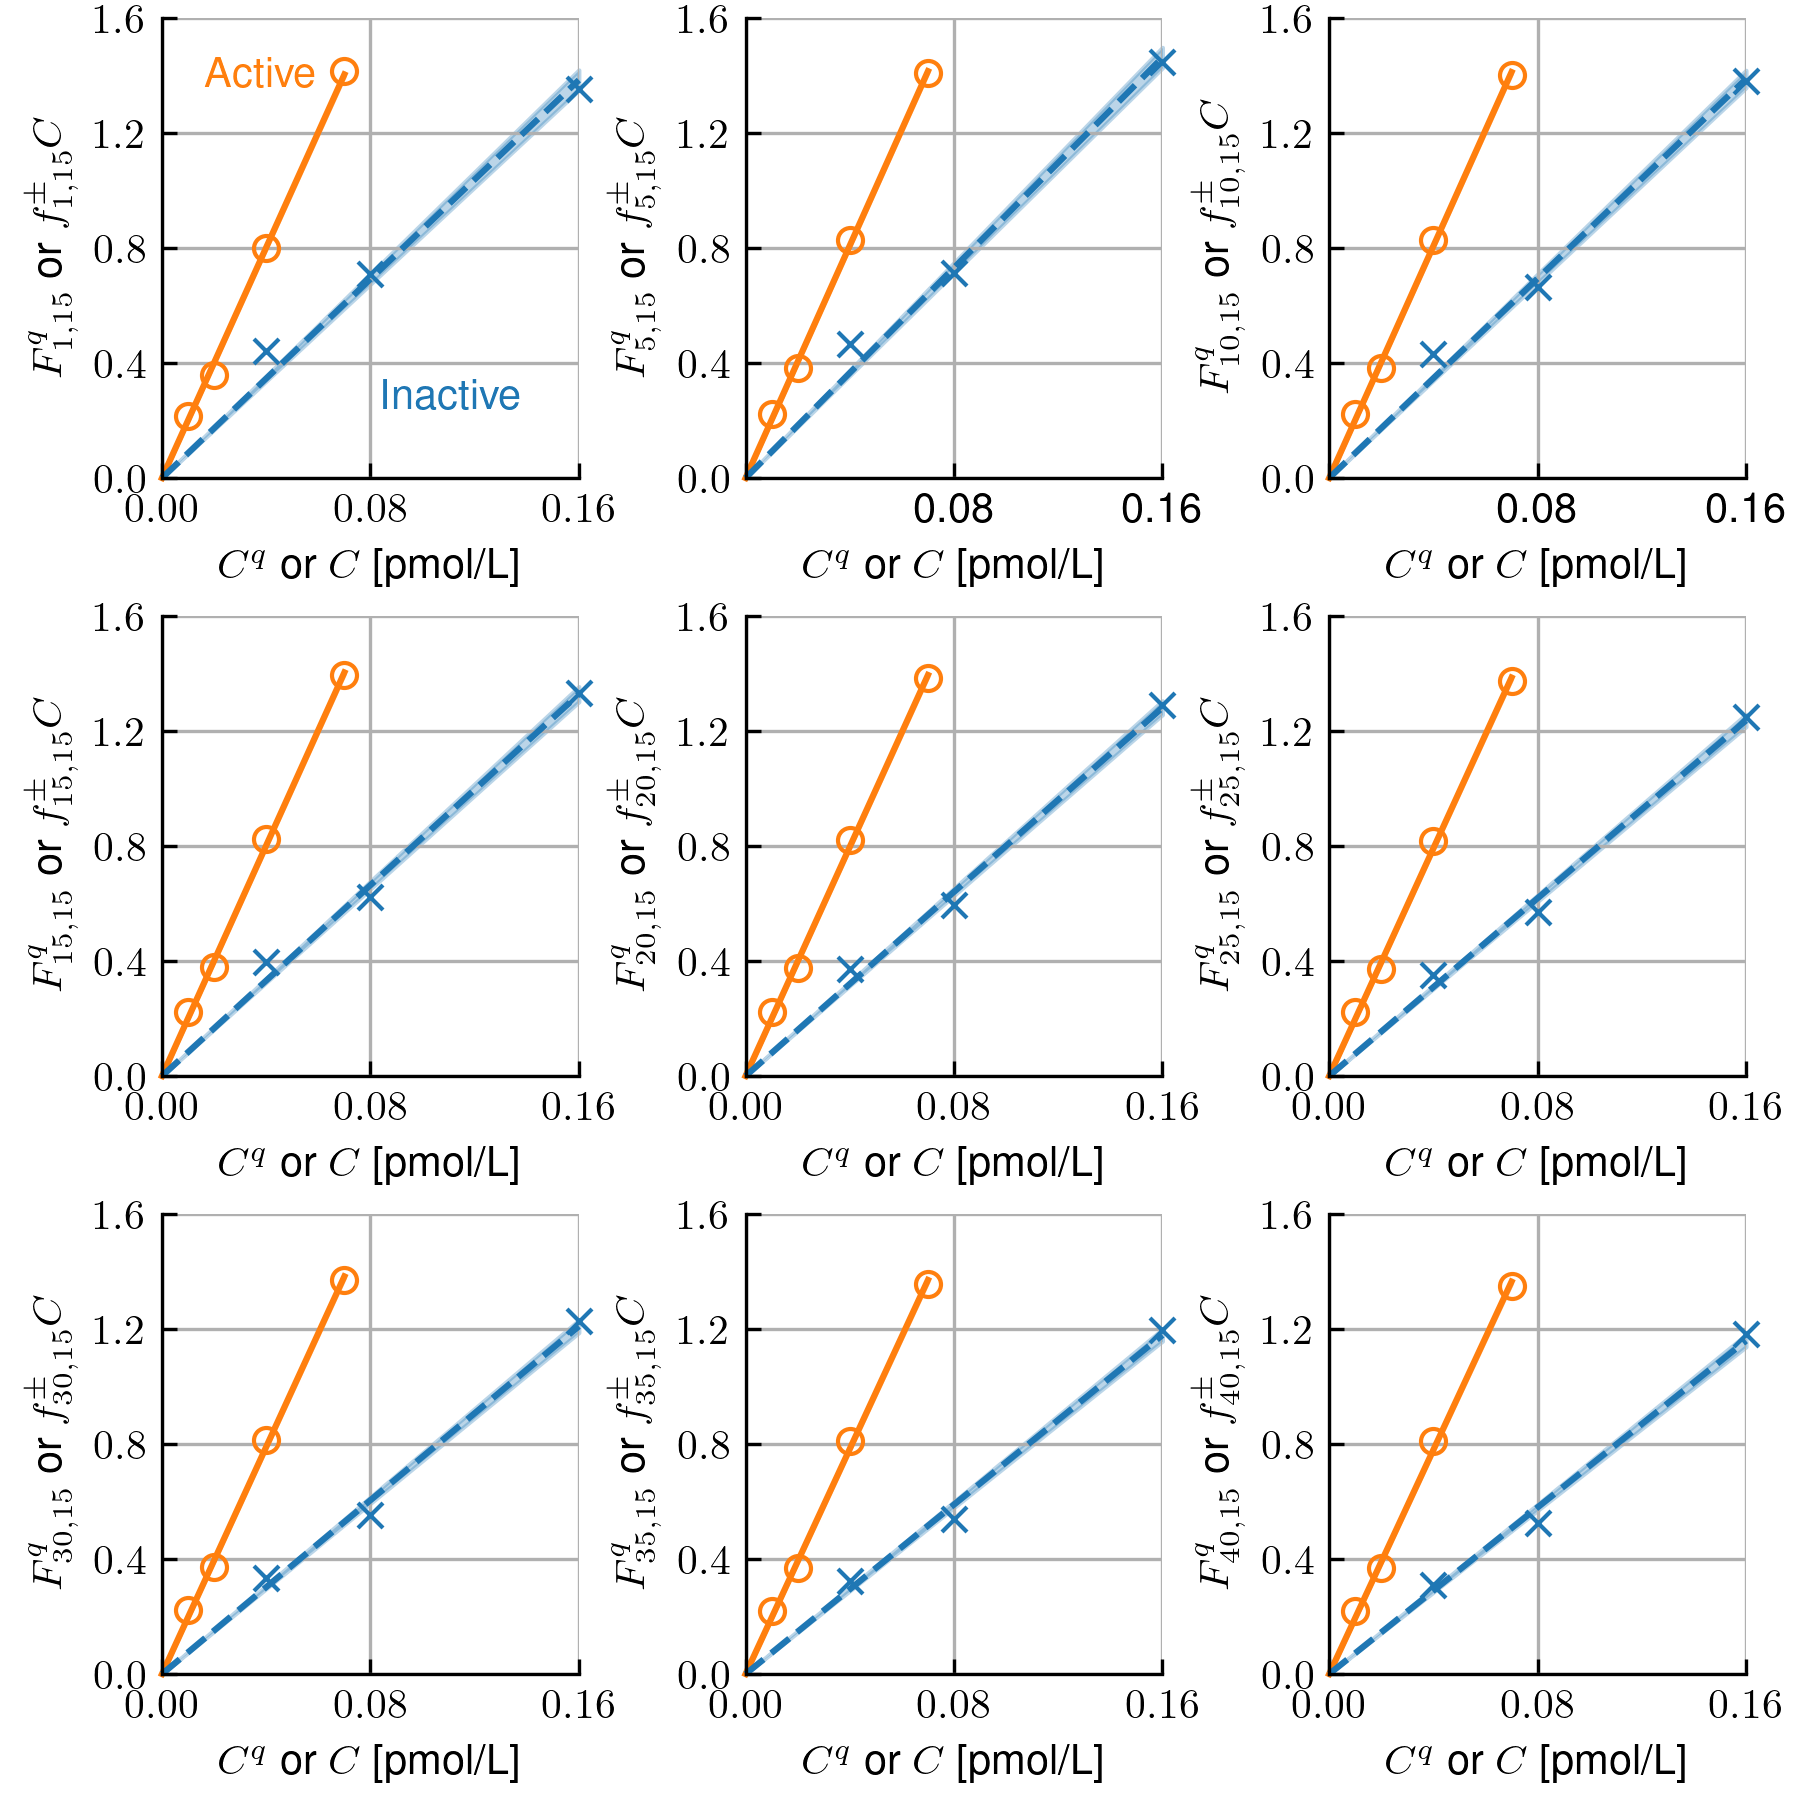
\includegraphics{si-figs/FigS15.png}
                    \caption{
                        As Figure~\ref{fig:S1} with well $w=15$ (or B3).
                    }
                \end{figure}
                \clearpage
    \begin{table}
        \caption{Molar Fluorescence Parameters for Well B3 ($w=15$)}
        \centering
        \begin{tabular}{c|ll|ll}
            Cycle & \multicolumn{2}{c|}{Inactive} & \multicolumn{2}{c}{Active} \\
            \hline
            $i$ & $f_{i,15}^{-}$ & $\sigma_{i,15}^{-}$ &  $f_{i,15}^{+}$ & $\sigma_{i,15}^{+}$ \\
            \hline
    1 & 8.65 & 0.073 & 20.05 & 0.027 \\
2 & 9.07 & 0.074 & 19.86 & 0.019 \\
3 & 9.21 & 0.075 & 20.07 & 0.021 \\
4 & 9.19 & 0.075 & 20.19 & 0.020 \\
5 & 9.14 & 0.074 & 20.21 & 0.021 \\
6 & 9.04 & 0.072 & 20.24 & 0.021 \\
7 & 8.95 & 0.069 & 20.22 & 0.021 \\
8 & 8.86 & 0.067 & 20.22 & 0.021 \\
9 & 8.78 & 0.065 & 20.21 & 0.022 \\
10 & 8.67 & 0.063 & 20.17 & 0.022 \\
11 & 8.59 & 0.061 & 20.17 & 0.023 \\
12 & 8.51 & 0.059 & 20.15 & 0.023 \\
13 & 8.44 & 0.058 & 20.11 & 0.023 \\
14 & 8.36 & 0.057 & 20.08 & 0.024 \\
15 & 8.30 & 0.055 & 20.05 & 0.024 \\
16 & 8.23 & 0.053 & 20.03 & 0.024 \\
17 & 8.16 & 0.052 & 20.03 & 0.024 \\
18 & 8.11 & 0.052 & 20.00 & 0.024 \\
19 & 8.06 & 0.051 & 19.96 & 0.025 \\
20 & 8.01 & 0.050 & 19.92 & 0.024 \\
21 & 7.95 & 0.049 & 19.91 & 0.024 \\
22 & 7.90 & 0.049 & 19.89 & 0.024 \\
23 & 7.90 & 0.049 & 19.85 & 0.024 \\
24 & 7.80 & 0.046 & 19.84 & 0.024 \\
25 & 7.73 & 0.045 & 19.79 & 0.026 \\
26 & 7.69 & 0.045 & 19.81 & 0.024 \\
27 & 7.65 & 0.045 & 19.80 & 0.025 \\
28 & 7.64 & 0.046 & 19.85 & 0.024 \\
29 & 7.60 & 0.045 & 19.79 & 0.024 \\
30 & 7.56 & 0.045 & 19.75 & 0.025 \\
31 & 7.50 & 0.044 & 19.87 & 0.023 \\
32 & 7.45 & 0.045 & 19.80 & 0.024 \\
33 & 7.41 & 0.044 & 19.74 & 0.023 \\
34 & 7.38 & 0.041 & 19.65 & 0.025 \\
35 & 7.37 & 0.043 & 19.58 & 0.026 \\
36 & 7.33 & 0.041 & 19.53 & 0.026 \\
37 & 7.34 & 0.045 & 19.86 & 0.022 \\
38 & 7.31 & 0.044 & 19.65 & 0.023 \\
39 & 7.27 & 0.044 & 19.59 & 0.027 \\
40 & 7.24 & 0.044 & 19.49 & 0.028 \\
41 & 7.21 & 0.045 & 19.39 & 0.028 \\
42 & 7.20 & 0.047 & 19.36 & 0.029 \\
43 & 7.24 & 0.050 & 19.63 & 0.025 \\
44 & 7.18 & 0.050 & 19.44 & 0.025 \\
45 & 7.11 & 0.048 & 19.56 & 0.027 \\
               \hline
        \end{tabular}
    \end{table}
    \clearpage

                \begin{figure}
                    \centering
                    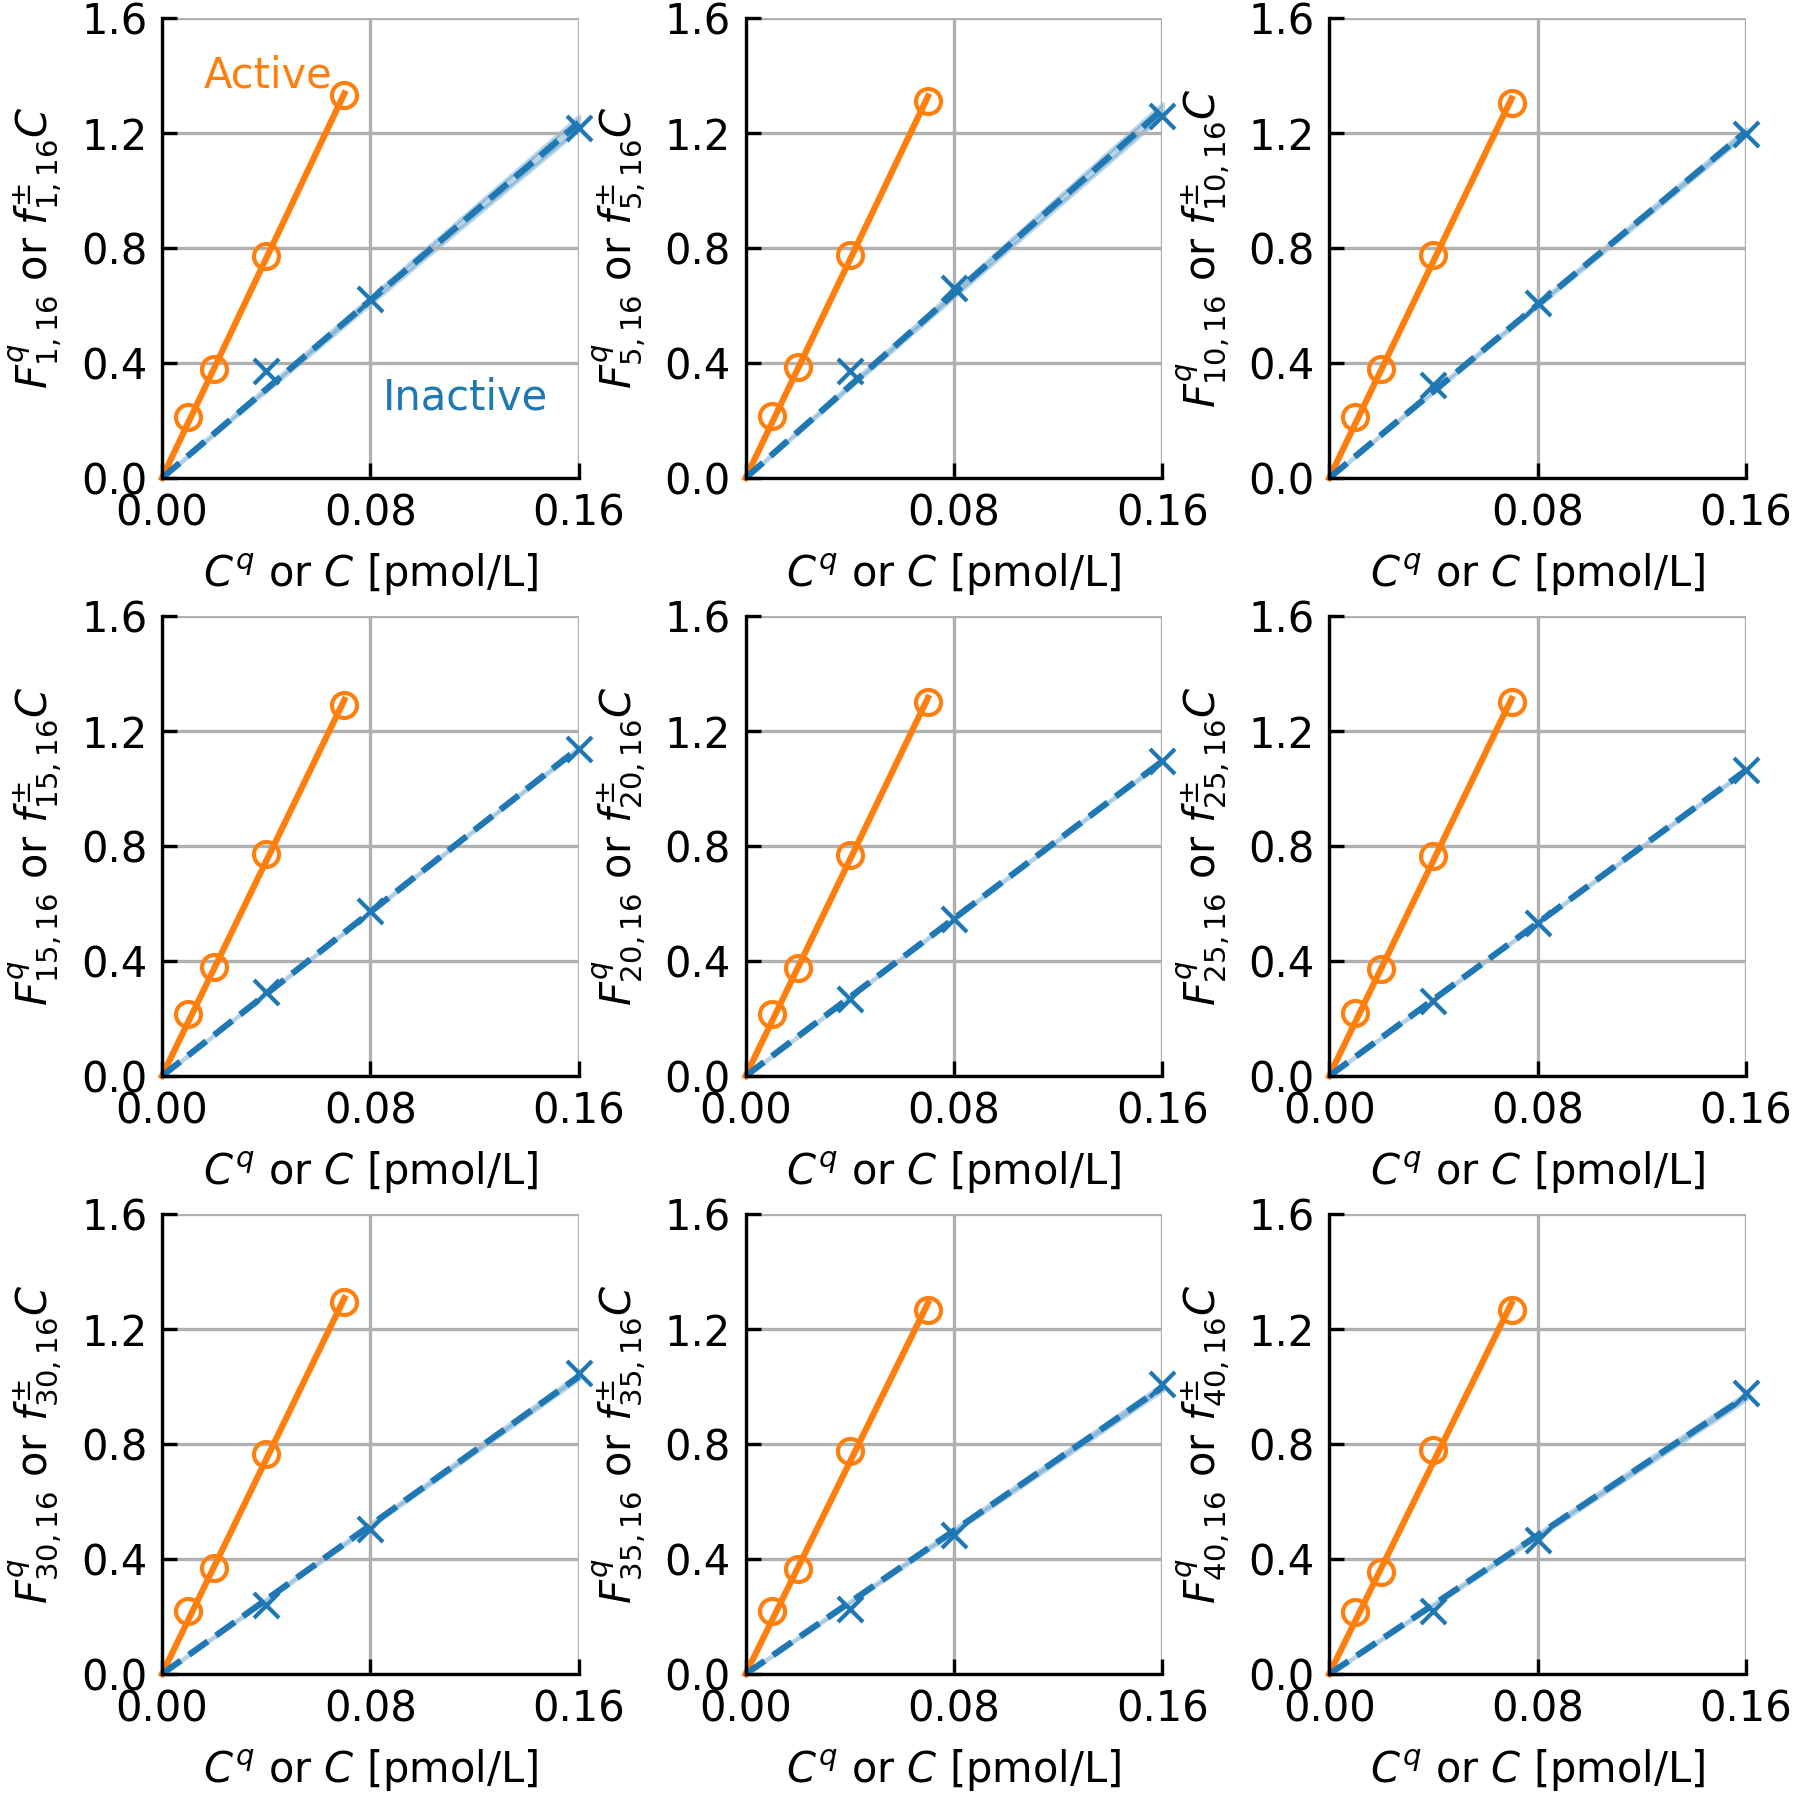
\includegraphics{si-figs/FigS16.png}
                    \caption{
                        As Figure~\ref{fig:S1} with well $w=16$ (or B4).
                    }
                \end{figure}
                \clearpage
    \begin{table}
        \caption{Molar Fluorescence Parameters for Well B4 ($w=16$)}
        \centering
        \begin{tabular}{c|ll|ll}
            Cycle & \multicolumn{2}{c|}{Inactive} & \multicolumn{2}{c}{Active} \\
            \hline
            $i$ & $f_{i,16}^{-}$ & $\sigma_{i,16}^{-}$ &  $f_{i,16}^{+}$ & $\sigma_{i,16}^{+}$ \\
            \hline
    1 & 7.72 & 0.047 & 19.11 & 0.013 \\
2 & 8.01 & 0.048 & 18.83 & 0.014 \\
3 & 8.13 & 0.047 & 18.92 & 0.017 \\
4 & 8.09 & 0.046 & 18.91 & 0.019 \\
5 & 8.01 & 0.043 & 18.96 & 0.020 \\
6 & 7.91 & 0.038 & 18.97 & 0.020 \\
7 & 7.82 & 0.032 & 18.93 & 0.020 \\
8 & 7.71 & 0.028 & 18.93 & 0.020 \\
9 & 7.62 & 0.023 & 18.88 & 0.020 \\
10 & 7.53 & 0.019 & 18.85 & 0.021 \\
11 & 7.44 & 0.015 & 18.84 & 0.021 \\
12 & 7.36 & 0.012 & 18.82 & 0.021 \\
13 & 7.282 & 0.0095 & 18.76 & 0.022 \\
14 & 7.195 & 0.0080 & 18.72 & 0.024 \\
15 & 7.132 & 0.0054 & 18.69 & 0.024 \\
16 & 7.051 & 0.0041 & 18.80 & 0.020 \\
17 & 6.984 & 0.0032 & 18.84 & 0.019 \\
18 & 6.953 & 0.0014 & 18.88 & 0.018 \\
19 & 6.9002 & 0.00057 & 18.83 & 0.019 \\
20 & 6.845 & 0.0040 & 18.79 & 0.020 \\
21 & 6.815 & 0.0064 & 18.82 & 0.024 \\
22 & 6.756 & 0.0082 & 18.78 & 0.022 \\
23 & 6.714 & 0.0067 & 18.73 & 0.022 \\
24 & 6.70 & 0.012 & 18.80 & 0.021 \\
25 & 6.648 & 0.0048 & 18.74 & 0.022 \\
26 & 6.601 & 0.0089 & 18.69 & 0.023 \\
27 & 6.59 & 0.016 & 18.67 & 0.022 \\
28 & 6.55 & 0.014 & 18.65 & 0.023 \\
29 & 6.55 & 0.017 & 18.65 & 0.024 \\
30 & 6.47 & 0.017 & 18.67 & 0.023 \\
31 & 6.40 & 0.014 & 18.74 & 0.022 \\
32 & 6.34 & 0.013 & 18.68 & 0.024 \\
33 & 6.29 & 0.020 & 18.91 & 0.021 \\
34 & 6.31 & 0.024 & 18.79 & 0.024 \\
35 & 6.23 & 0.021 & 18.43 & 0.032 \\
36 & 6.19 & 0.019 & 18.48 & 0.031 \\
37 & 6.15 & 0.023 & 18.45 & 0.031 \\
38 & 6.09 & 0.024 & 18.53 & 0.038 \\
39 & 6.06 & 0.021 & 18.47 & 0.036 \\
40 & 6.03 & 0.022 & 18.43 & 0.034 \\
41 & 6.03 & 0.023 & 18.38 & 0.033 \\
42 & 6.03 & 0.023 & 18.39 & 0.034 \\
43 & 6.07 & 0.025 & 18.27 & 0.034 \\
44 & 5.95 & 0.023 & 18.28 & 0.033 \\
45 & 5.96 & 0.022 & 18.26 & 0.032 \\
               \hline
        \end{tabular}
    \end{table}
    \clearpage

                \begin{figure}
                    \centering
                    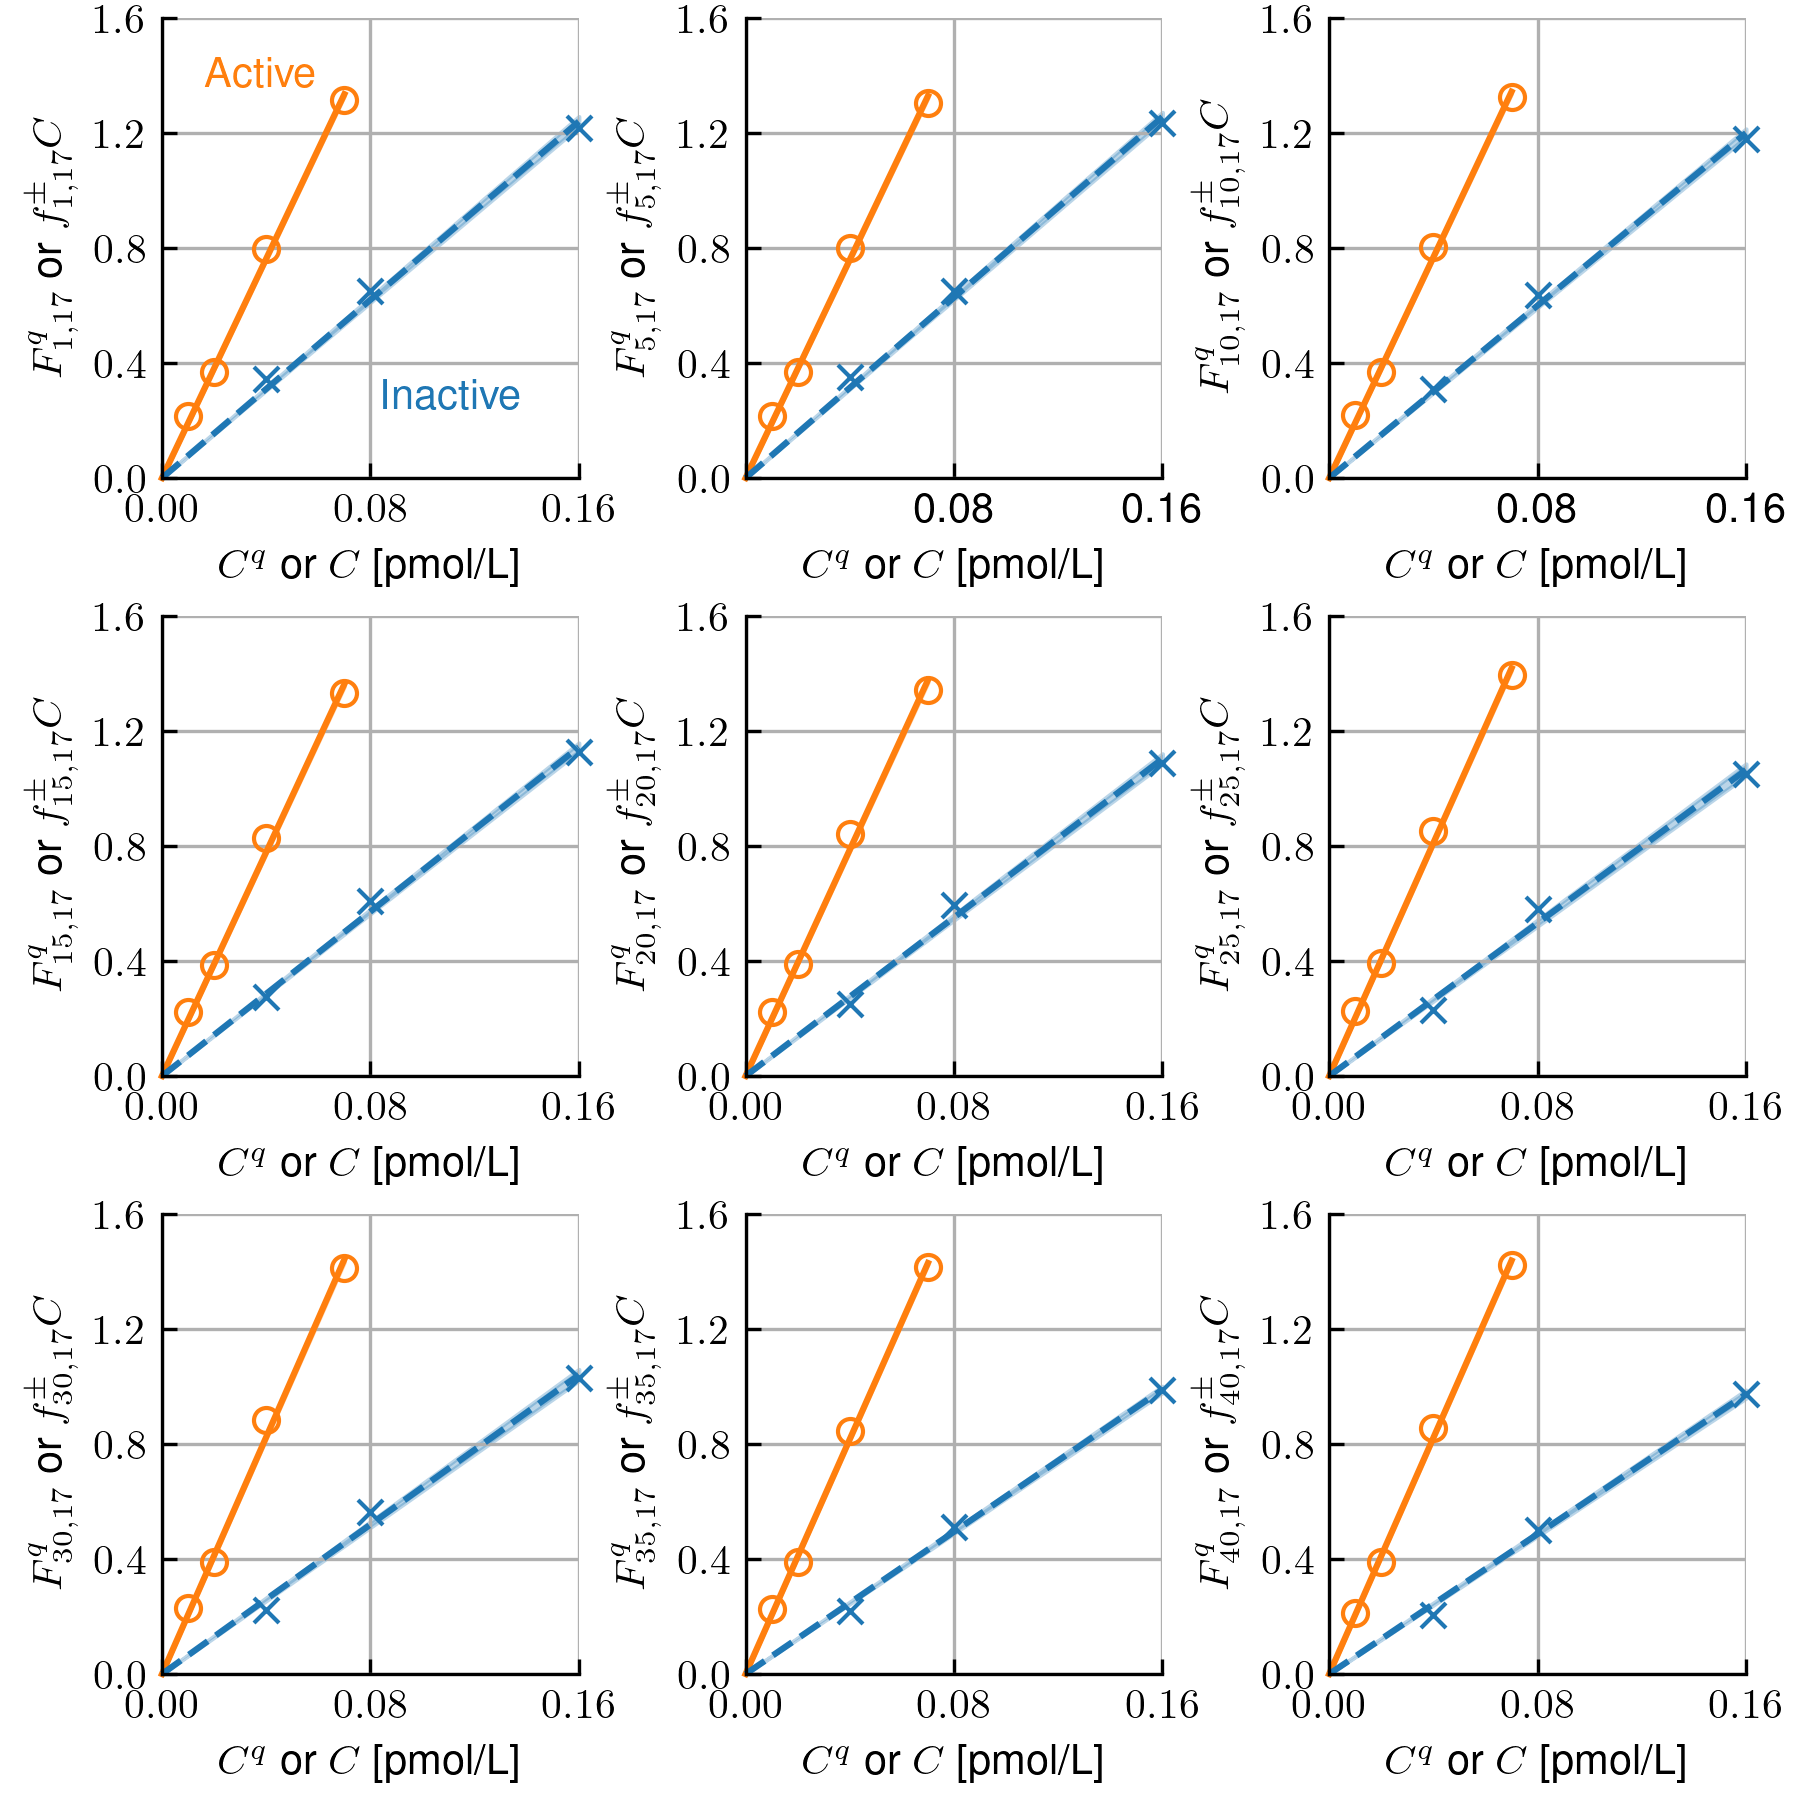
\includegraphics{si-figs/FigS17.png}
                    \caption{
                        As Figure~\ref{fig:S1} with well $w=17$ (or B5).
                    }
                \end{figure}
                \clearpage
    \begin{table}
        \caption{Molar Fluorescence Parameters for Well B5 ($w=17$)}
        \centering
        \begin{tabular}{c|ll|ll}
            Cycle & \multicolumn{2}{c|}{Inactive} & \multicolumn{2}{c}{Active} \\
            \hline
            $i$ & $f_{i,17}^{-}$ & $\sigma_{i,17}^{-}$ &  $f_{i,17}^{+}$ & $\sigma_{i,17}^{+}$ \\
            \hline
    1 & 7.75 & 0.037 & 19.07 & 0.027 \\
2 & 7.63 & 0.042 & 18.56 & 0.029 \\
3 & 7.81 & 0.040 & 18.67 & 0.030 \\
4 & 7.87 & 0.037 & 18.83 & 0.030 \\
5 & 7.85 & 0.033 & 18.98 & 0.030 \\
6 & 7.78 & 0.029 & 19.05 & 0.030 \\
7 & 7.68 & 0.024 & 19.07 & 0.030 \\
8 & 7.64 & 0.027 & 19.11 & 0.029 \\
9 & 7.57 & 0.030 & 19.14 & 0.029 \\
10 & 7.50 & 0.030 & 19.19 & 0.029 \\
11 & 7.42 & 0.029 & 19.22 & 0.032 \\
12 & 7.34 & 0.028 & 19.29 & 0.035 \\
13 & 7.28 & 0.029 & 19.34 & 0.036 \\
14 & 7.21 & 0.030 & 19.44 & 0.036 \\
15 & 7.15 & 0.030 & 19.47 & 0.037 \\
16 & 7.10 & 0.032 & 19.52 & 0.037 \\
17 & 7.05 & 0.033 & 19.54 & 0.038 \\
18 & 7.00 & 0.034 & 19.60 & 0.038 \\
19 & 6.94 & 0.034 & 19.64 & 0.039 \\
20 & 6.89 & 0.037 & 19.68 & 0.040 \\
21 & 6.84 & 0.039 & 19.85 & 0.037 \\
22 & 6.81 & 0.039 & 19.89 & 0.037 \\
23 & 6.76 & 0.040 & 19.97 & 0.037 \\
24 & 6.63 & 0.044 & 20.19 & 0.032 \\
25 & 6.65 & 0.044 & 20.26 & 0.032 \\
26 & 6.59 & 0.045 & 20.32 & 0.033 \\
27 & 6.57 & 0.043 & 20.38 & 0.036 \\
28 & 6.57 & 0.042 & 20.48 & 0.041 \\
29 & 6.49 & 0.043 & 20.52 & 0.042 \\
30 & 6.50 & 0.041 & 20.60 & 0.043 \\
31 & 6.44 & 0.039 & 20.68 & 0.045 \\
32 & 6.40 & 0.040 & 20.67 & 0.047 \\
33 & 6.24 & 0.022 & 20.73 & 0.048 \\
34 & 6.21 & 0.023 & 20.43 & 0.023 \\
35 & 6.18 & 0.024 & 20.42 & 0.025 \\
36 & 6.15 & 0.026 & 20.41 & 0.027 \\
37 & 6.10 & 0.026 & 20.41 & 0.027 \\
38 & 6.13 & 0.027 & 20.46 & 0.024 \\
39 & 6.10 & 0.028 & 20.52 & 0.025 \\
40 & 6.08 & 0.029 & 20.54 & 0.026 \\
41 & 6.30 & 0.036 & 20.57 & 0.026 \\
42 & 6.28 & 0.038 & 20.56 & 0.028 \\
43 & 6.28 & 0.039 & 20.59 & 0.029 \\
44 & 6.27 & 0.040 & 20.58 & 0.034 \\
45 & 6.24 & 0.043 & 20.67 & 0.035 \\
               \hline
        \end{tabular}
    \end{table}
    \clearpage

                \begin{figure}
                    \centering
                    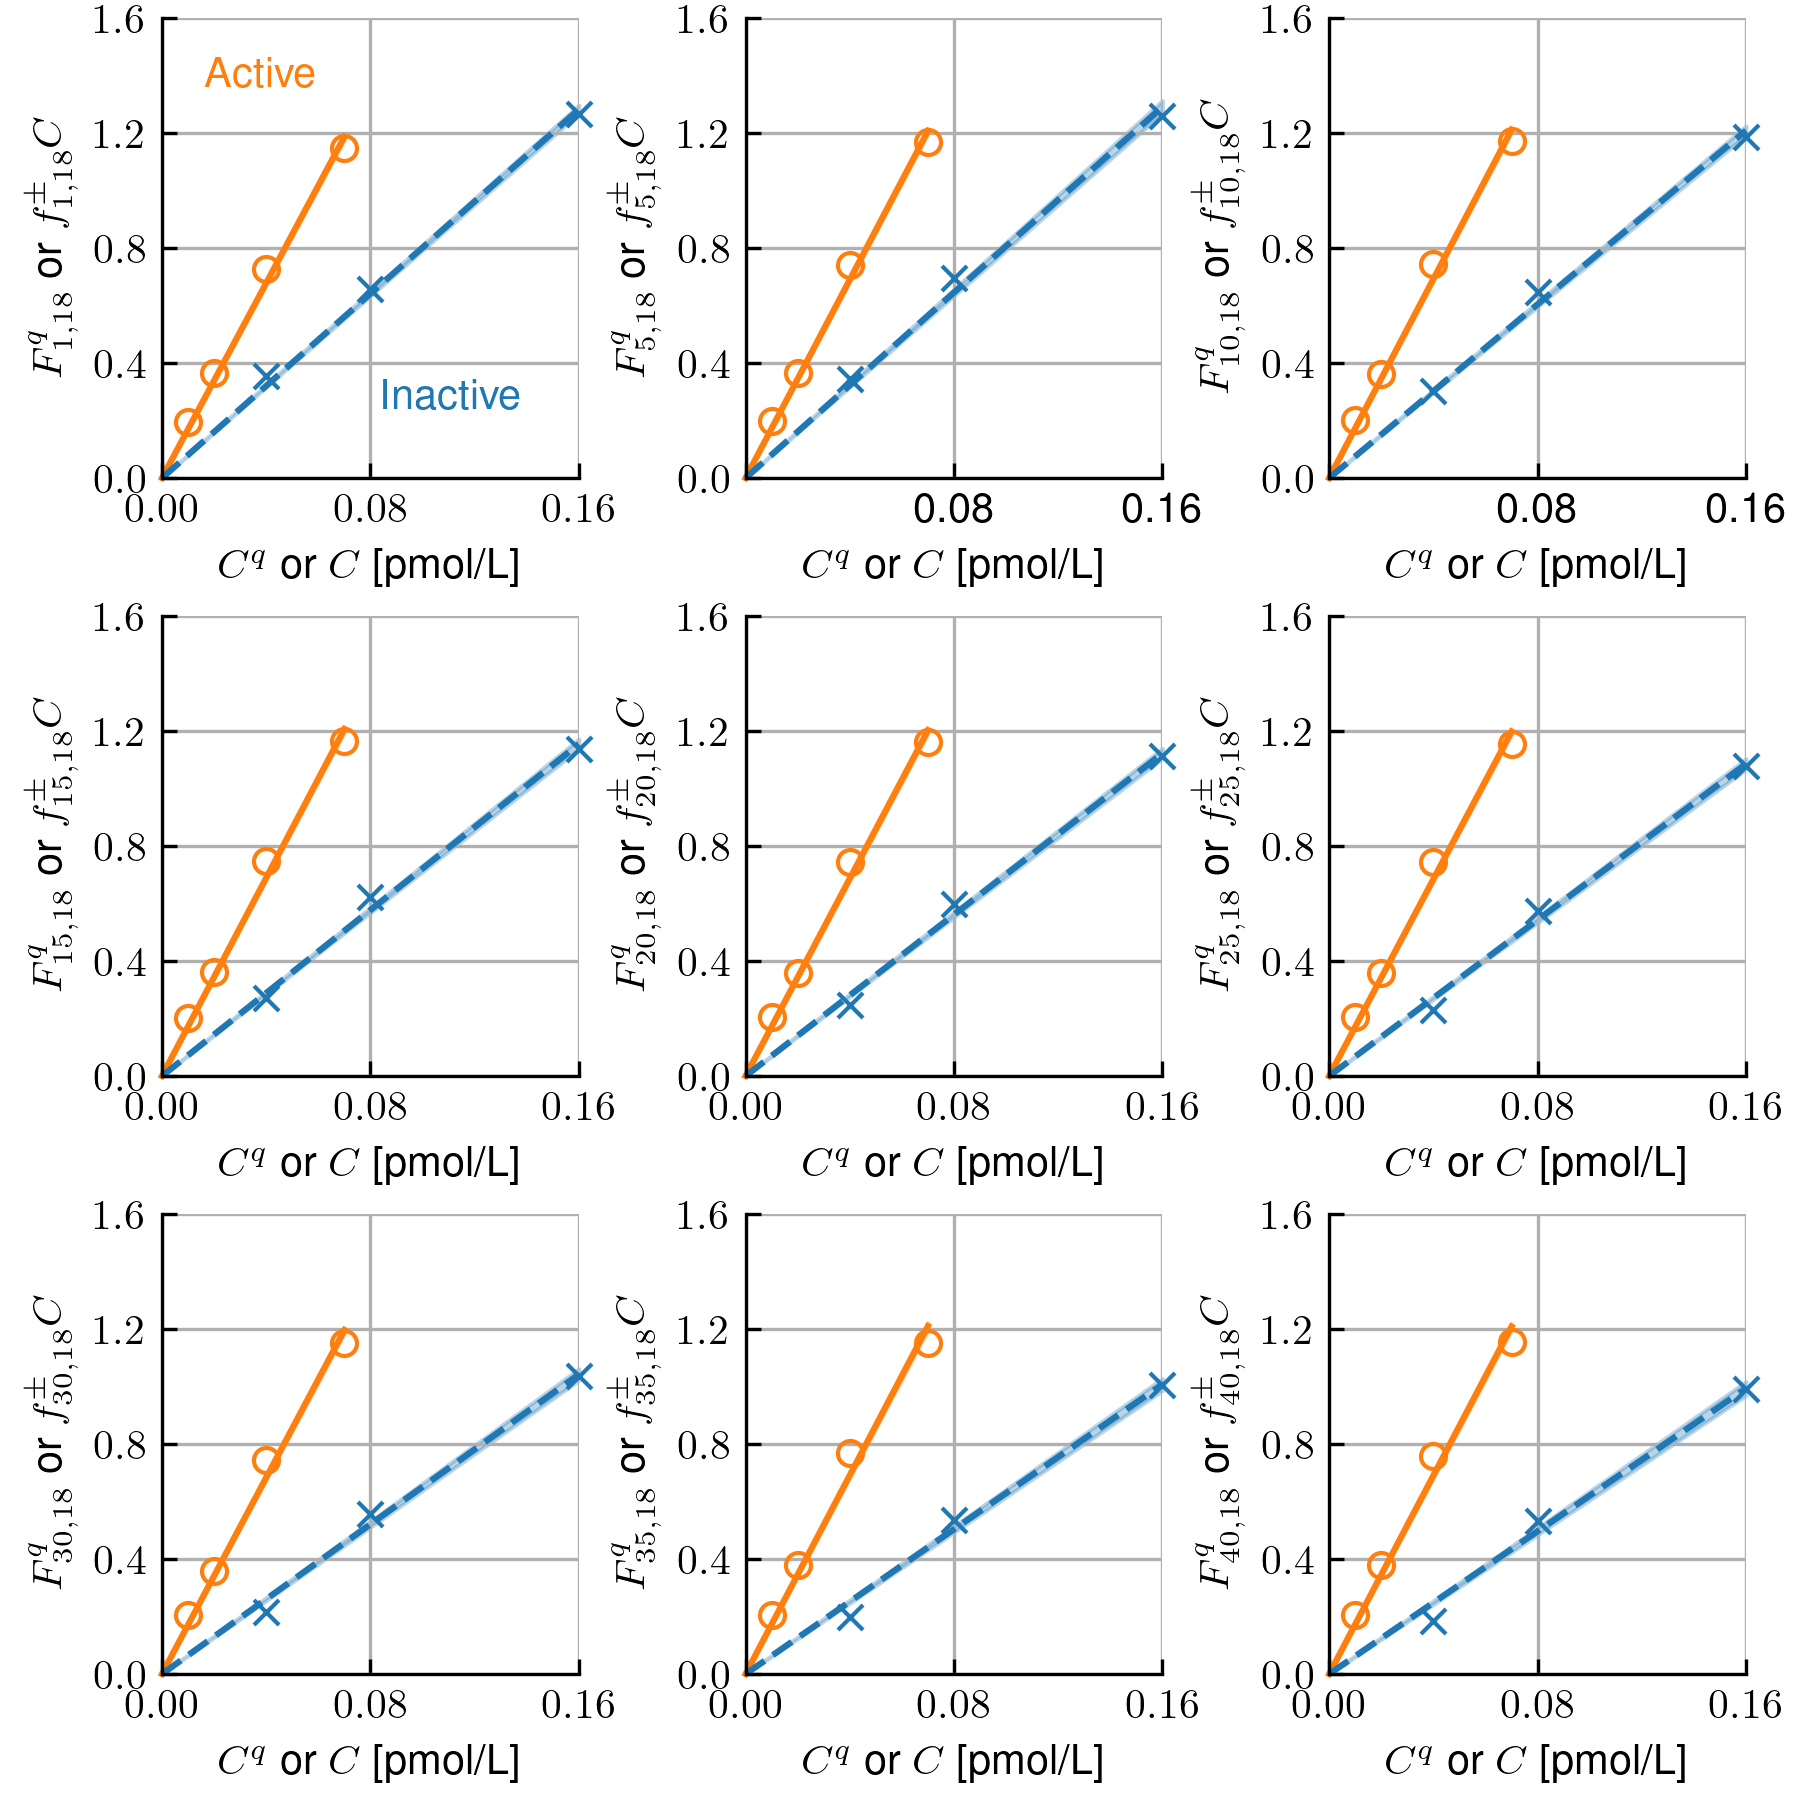
\includegraphics{si-figs/FigS18.png}
                    \caption{
                        As Figure~\ref{fig:S1} with well $w=18$ (or B6).
                    }
                \end{figure}
                \clearpage
    \begin{table}
        \caption{Molar Fluorescence Parameters for Well B6 ($w=18$)}
        \centering
        \begin{tabular}{c|ll|ll}
            Cycle & \multicolumn{2}{c|}{Inactive} & \multicolumn{2}{c}{Active} \\
            \hline
            $i$ & $f_{i,18}^{-}$ & $\sigma_{i,18}^{-}$ &  $f_{i,18}^{+}$ & $\sigma_{i,18}^{+}$ \\
            \hline
    1 & 8.01 & 0.030 & 16.95 & 0.043 \\
2 & 7.89 & 0.044 & 16.76 & 0.042 \\
3 & 8.05 & 0.043 & 17.03 & 0.039 \\
4 & 8.09 & 0.044 & 17.14 & 0.042 \\
5 & 8.07 & 0.046 & 17.24 & 0.041 \\
6 & 7.96 & 0.044 & 17.29 & 0.042 \\
7 & 7.86 & 0.040 & 17.30 & 0.042 \\
8 & 7.74 & 0.037 & 17.30 & 0.043 \\
9 & 7.64 & 0.033 & 17.31 & 0.044 \\
10 & 7.55 & 0.033 & 17.30 & 0.043 \\
11 & 7.50 & 0.035 & 17.29 & 0.044 \\
12 & 7.41 & 0.037 & 17.31 & 0.044 \\
13 & 7.34 & 0.037 & 17.26 & 0.044 \\
14 & 7.26 & 0.037 & 17.26 & 0.045 \\
15 & 7.22 & 0.036 & 17.23 & 0.045 \\
16 & 7.17 & 0.035 & 17.22 & 0.045 \\
17 & 7.11 & 0.035 & 17.20 & 0.045 \\
18 & 7.10 & 0.034 & 17.19 & 0.046 \\
19 & 7.06 & 0.034 & 17.17 & 0.046 \\
20 & 7.01 & 0.036 & 17.17 & 0.046 \\
21 & 6.95 & 0.035 & 17.13 & 0.046 \\
22 & 6.90 & 0.036 & 17.02 & 0.050 \\
23 & 6.90 & 0.036 & 17.11 & 0.047 \\
24 & 6.85 & 0.039 & 17.12 & 0.047 \\
25 & 6.78 & 0.038 & 17.11 & 0.048 \\
26 & 6.74 & 0.039 & 17.11 & 0.048 \\
27 & 6.75 & 0.038 & 17.13 & 0.050 \\
28 & 6.64 & 0.039 & 17.10 & 0.048 \\
29 & 6.57 & 0.042 & 17.09 & 0.048 \\
30 & 6.51 & 0.041 & 17.08 & 0.049 \\
31 & 6.46 & 0.040 & 17.10 & 0.052 \\
32 & 6.44 & 0.041 & 17.27 & 0.062 \\
33 & 6.44 & 0.041 & 17.22 & 0.059 \\
34 & 6.34 & 0.041 & 17.33 & 0.066 \\
35 & 6.29 & 0.043 & 17.29 & 0.062 \\
36 & 6.29 & 0.045 & 17.25 & 0.062 \\
37 & 6.35 & 0.046 & 17.25 & 0.060 \\
38 & 6.32 & 0.047 & 17.25 & 0.060 \\
39 & 6.32 & 0.048 & 17.23 & 0.059 \\
40 & 6.21 & 0.050 & 17.26 & 0.056 \\
41 & 6.16 & 0.049 & 17.23 & 0.067 \\
42 & 6.13 & 0.046 & 17.78 & 0.055 \\
43 & 6.11 & 0.047 & 17.78 & 0.050 \\
44 & 6.11 & 0.047 & 17.75 & 0.049 \\
45 & 6.05 & 0.045 & 17.73 & 0.049 \\
               \hline
        \end{tabular}
    \end{table}
    \clearpage

                \begin{figure}
                    \centering
                    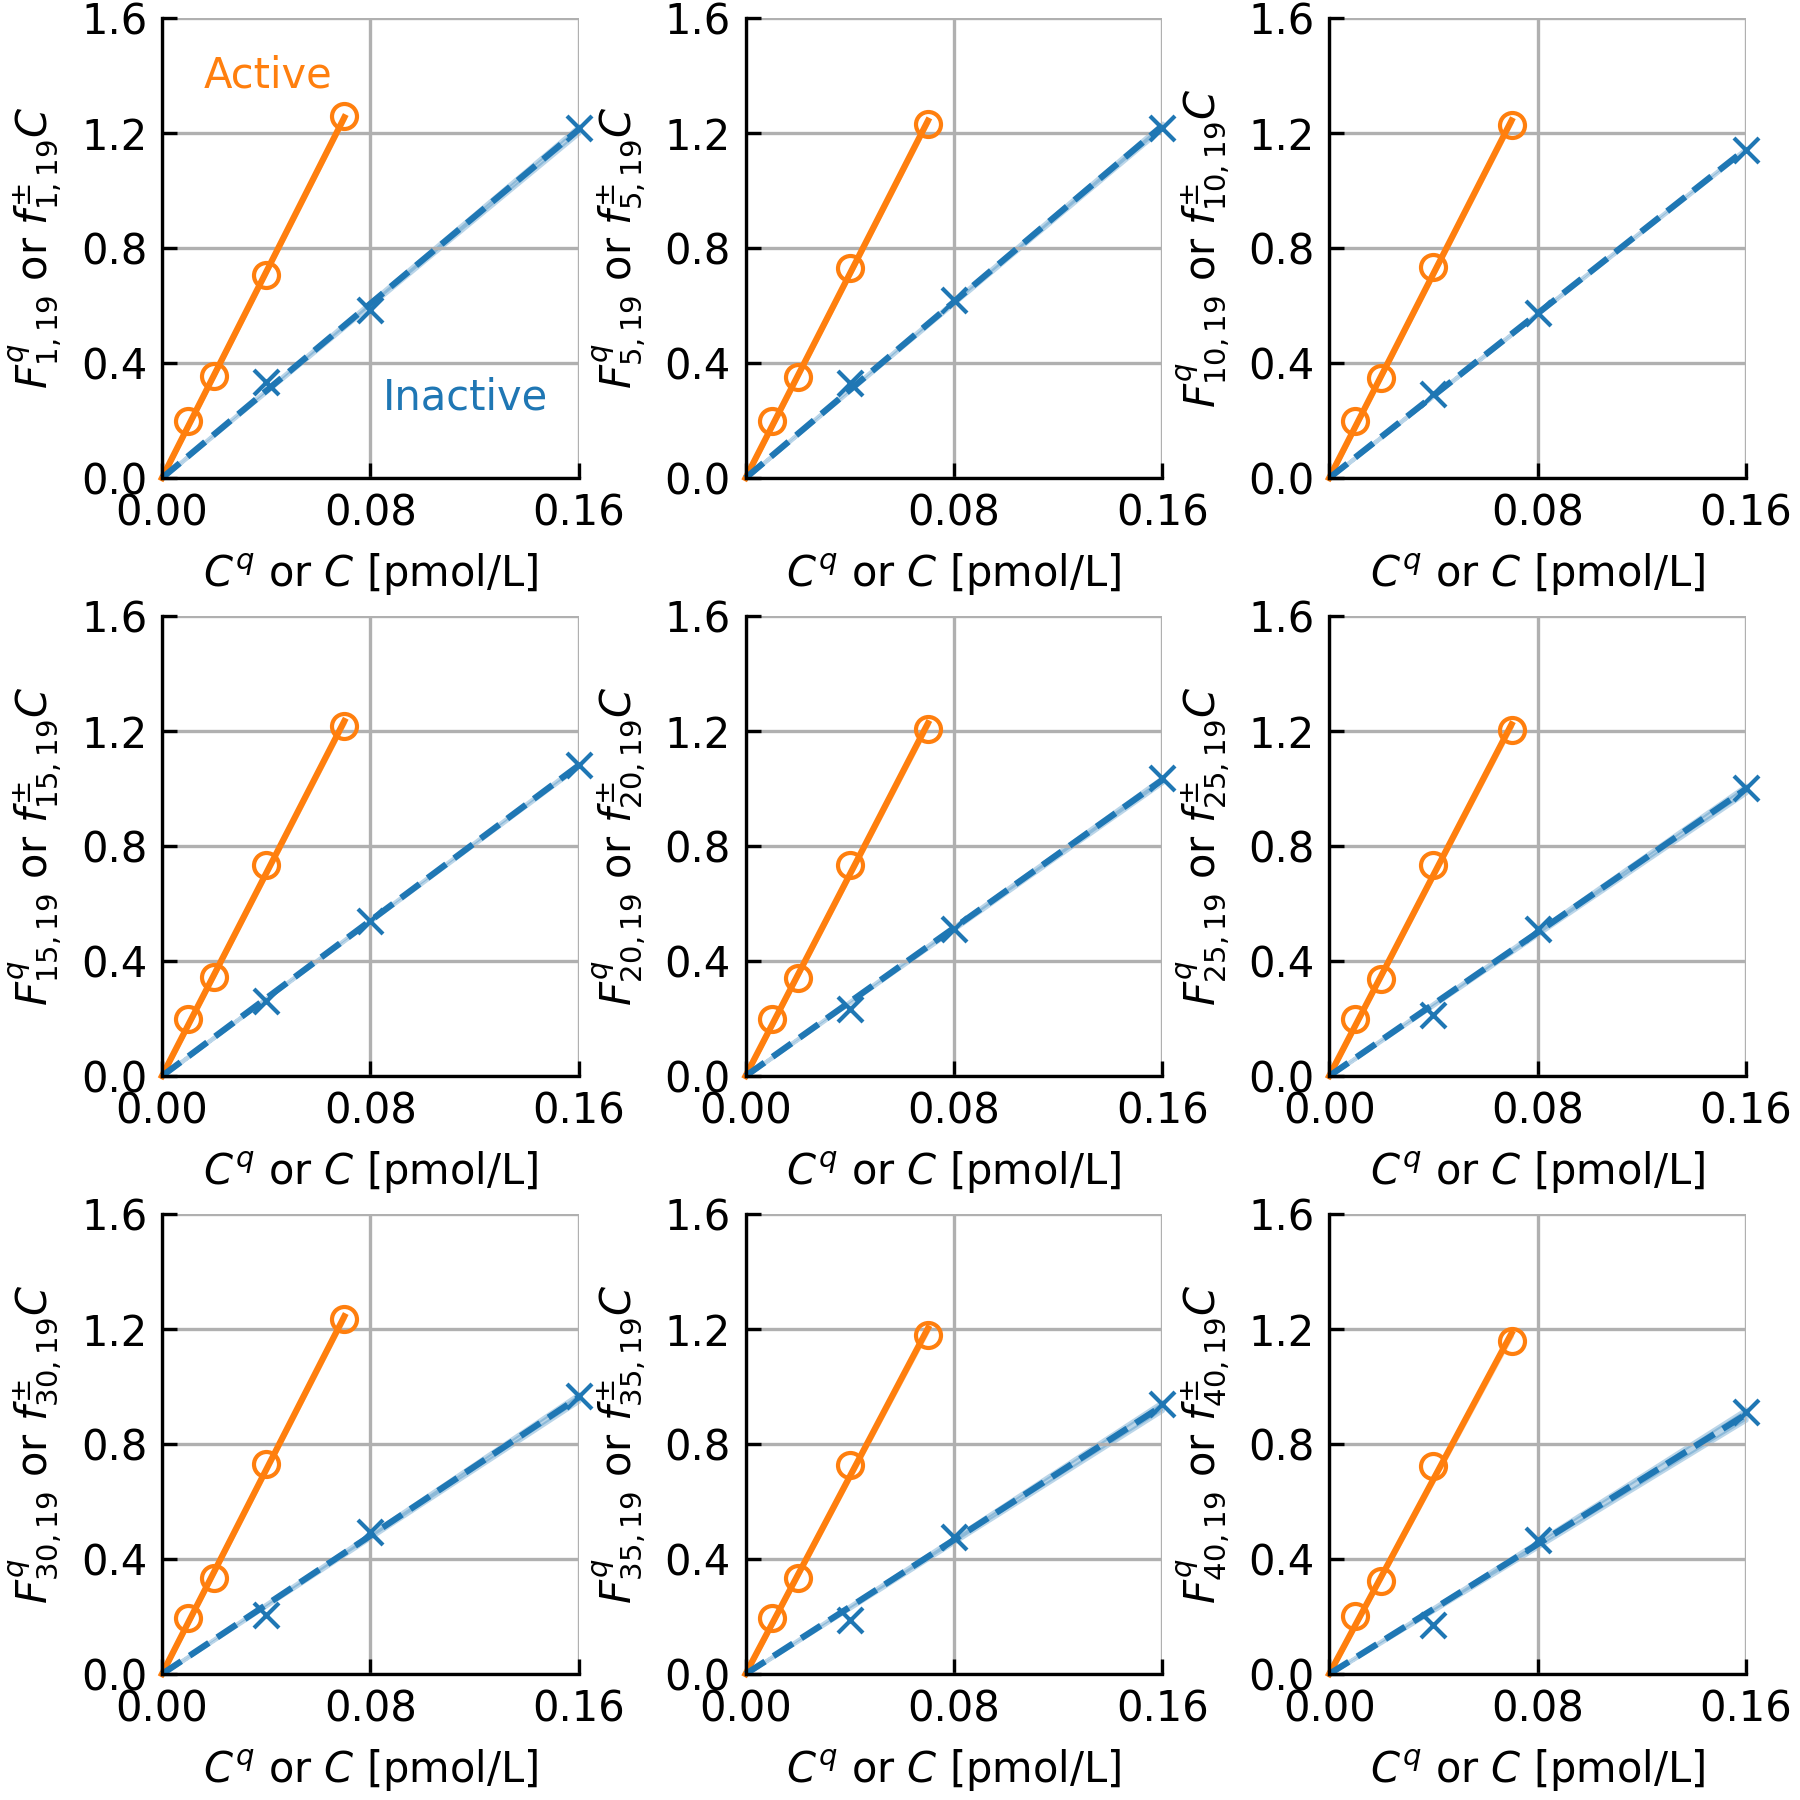
\includegraphics{si-figs/FigS19.png}
                    \caption{
                        As Figure~\ref{fig:S1} with well $w=19$ (or B7).
                    }
                \end{figure}
                \clearpage
    \begin{table}
        \caption{Molar Fluorescence Parameters for Well B7 ($w=19$)}
        \centering
        \begin{tabular}{c|ll|ll}
            Cycle & \multicolumn{2}{c|}{Inactive} & \multicolumn{2}{c}{Active} \\
            \hline
            $i$ & $f_{i,19}^{-}$ & $\sigma_{i,19}^{-}$ &  $f_{i,19}^{+}$ & $\sigma_{i,19}^{+}$ \\
            \hline
    1 & 7.58 & 0.027 & 17.92 & 0.014 \\
2 & 7.49 & 0.024 & 17.44 & 0.013 \\
3 & 7.65 & 0.022 & 17.66 & 0.014 \\
4 & 7.68 & 0.021 & 17.77 & 0.015 \\
5 & 7.66 & 0.019 & 17.75 & 0.018 \\
6 & 7.59 & 0.016 & 17.78 & 0.018 \\
7 & 7.46 & 0.015 & 17.78 & 0.019 \\
8 & 7.34 & 0.012 & 17.76 & 0.020 \\
9 & 7.254 & 0.0081 & 17.79 & 0.020 \\
10 & 7.153 & 0.0048 & 17.76 & 0.021 \\
11 & 7.071 & 0.0022 & 17.76 & 0.022 \\
12 & 6.978 & 0.0021 & 17.72 & 0.022 \\
13 & 6.915 & 0.0041 & 17.71 & 0.023 \\
14 & 6.843 & 0.0066 & 17.67 & 0.023 \\
15 & 6.755 & 0.0080 & 17.64 & 0.024 \\
16 & 6.69 & 0.010 & 17.61 & 0.024 \\
17 & 6.63 & 0.011 & 17.61 & 0.024 \\
18 & 6.54 & 0.013 & 17.57 & 0.026 \\
19 & 6.49 & 0.016 & 17.54 & 0.026 \\
20 & 6.44 & 0.019 & 17.53 & 0.027 \\
21 & 6.41 & 0.021 & 17.53 & 0.026 \\
22 & 6.39 & 0.023 & 17.50 & 0.027 \\
23 & 6.34 & 0.025 & 17.50 & 0.027 \\
24 & 6.29 & 0.027 & 17.49 & 0.027 \\
25 & 6.24 & 0.027 & 17.47 & 0.027 \\
26 & 6.21 & 0.027 & 17.45 & 0.027 \\
27 & 6.17 & 0.028 & 17.44 & 0.028 \\
28 & 6.11 & 0.024 & 17.44 & 0.027 \\
29 & 6.06 & 0.025 & 17.42 & 0.028 \\
30 & 6.02 & 0.027 & 17.77 & 0.021 \\
31 & 5.98 & 0.029 & 17.47 & 0.025 \\
32 & 5.94 & 0.029 & 17.40 & 0.026 \\
33 & 5.94 & 0.030 & 17.36 & 0.027 \\
34 & 5.88 & 0.031 & 17.25 & 0.029 \\
35 & 5.83 & 0.033 & 17.18 & 0.031 \\
36 & 5.78 & 0.037 & 17.12 & 0.032 \\
37 & 5.74 & 0.036 & 17.13 & 0.031 \\
38 & 5.71 & 0.038 & 17.16 & 0.032 \\
39 & 5.69 & 0.037 & 17.12 & 0.033 \\
40 & 5.64 & 0.040 & 16.93 & 0.038 \\
41 & 5.66 & 0.043 & 17.05 & 0.034 \\
42 & 5.61 & 0.041 & 17.00 & 0.035 \\
43 & 5.59 & 0.046 & 17.02 & 0.033 \\
44 & 5.51 & 0.041 & 16.97 & 0.035 \\
45 & 5.49 & 0.039 & 17.08 & 0.046 \\
               \hline
        \end{tabular}
    \end{table}
    \clearpage

                \begin{figure}
                    \centering
                    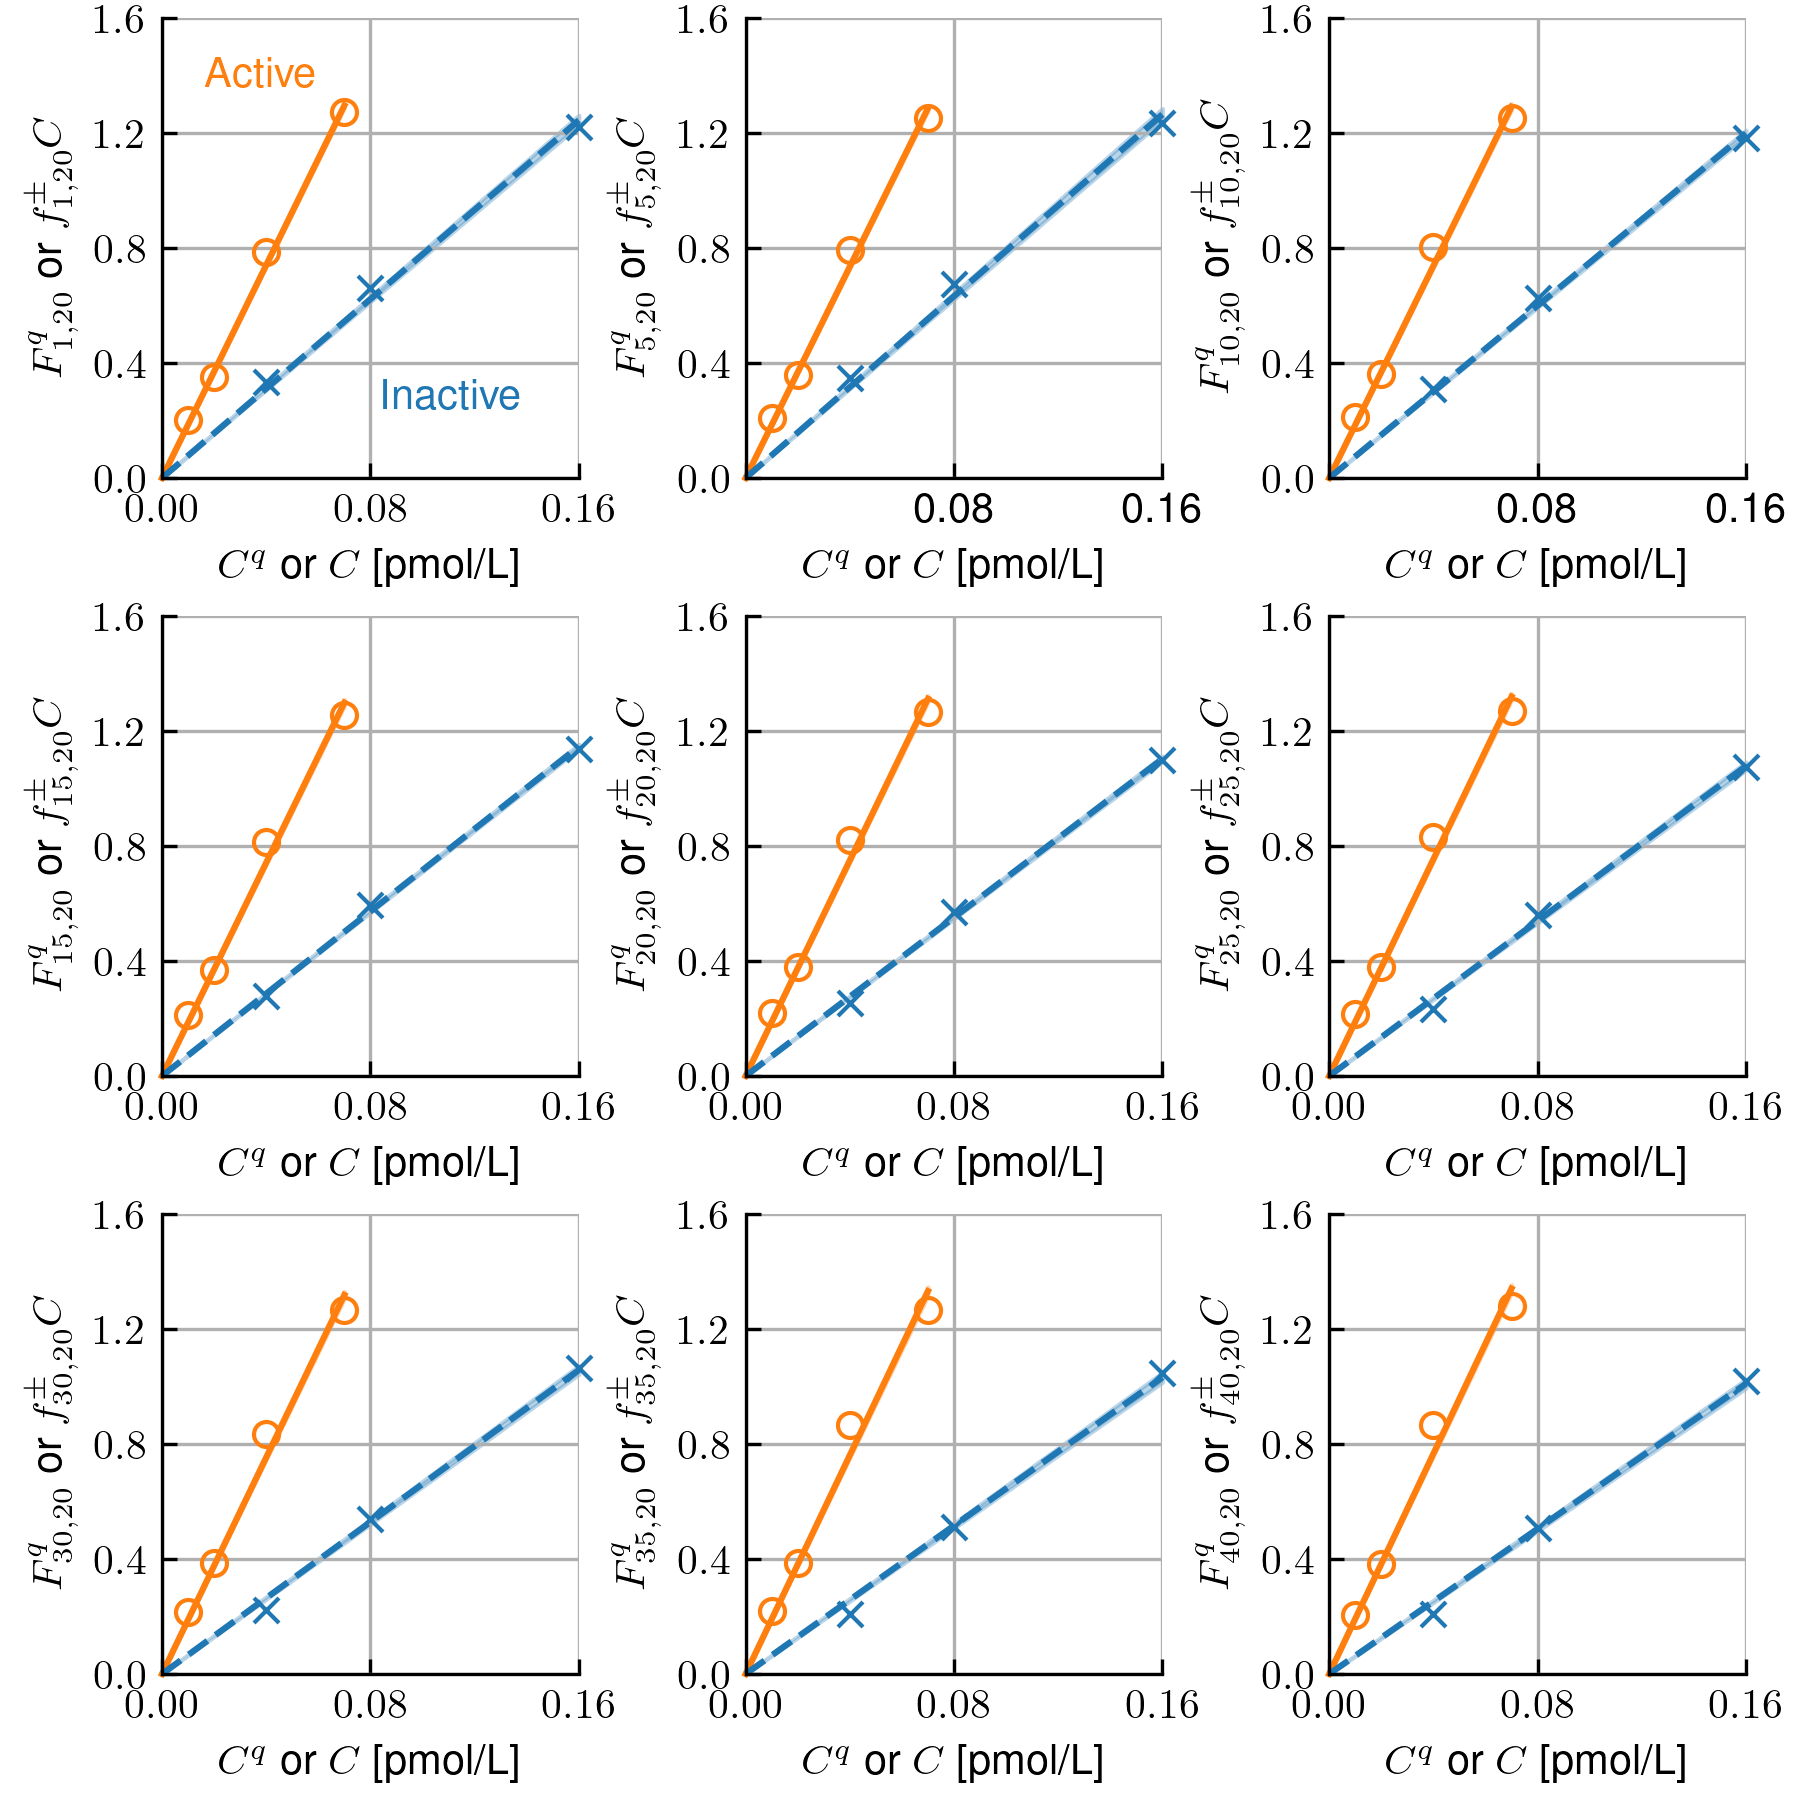
\includegraphics{si-figs/FigS20.png}
                    \caption{
                        As Figure~\ref{fig:S1} with well $w=20$ (or B8).
                    }
                \end{figure}
                \clearpage
    \begin{table}
        \caption{Molar Fluorescence Parameters for Well B8 ($w=20$)}
        \centering
        \begin{tabular}{c|ll|ll}
            Cycle & \multicolumn{2}{c|}{Inactive} & \multicolumn{2}{c}{Active} \\
            \hline
            $i$ & $f_{i,20}^{-}$ & $\sigma_{i,20}^{-}$ &  $f_{i,20}^{+}$ & $\sigma_{i,20}^{+}$ \\
            \hline
    1 & 7.78 & 0.036 & 18.51 & 0.033 \\
2 & 7.70 & 0.044 & 18.03 & 0.037 \\
3 & 7.89 & 0.043 & 18.22 & 0.038 \\
4 & 7.93 & 0.044 & 18.29 & 0.041 \\
5 & 7.90 & 0.043 & 18.37 & 0.041 \\
6 & 7.81 & 0.040 & 18.40 & 0.042 \\
7 & 7.73 & 0.034 & 18.41 & 0.043 \\
8 & 7.65 & 0.029 & 18.44 & 0.044 \\
9 & 7.56 & 0.026 & 18.43 & 0.045 \\
10 & 7.49 & 0.023 & 18.45 & 0.048 \\
11 & 7.42 & 0.020 & 18.52 & 0.047 \\
12 & 7.34 & 0.018 & 18.51 & 0.048 \\
13 & 7.28 & 0.018 & 18.51 & 0.049 \\
14 & 7.22 & 0.018 & 18.55 & 0.051 \\
15 & 7.16 & 0.017 & 18.55 & 0.051 \\
16 & 7.10 & 0.017 & 18.58 & 0.050 \\
17 & 7.04 & 0.019 & 18.64 & 0.051 \\
18 & 6.98 & 0.019 & 18.69 & 0.051 \\
19 & 6.94 & 0.018 & 18.71 & 0.052 \\
20 & 6.89 & 0.020 & 18.74 & 0.053 \\
21 & 6.86 & 0.023 & 18.85 & 0.053 \\
22 & 6.81 & 0.025 & 18.85 & 0.056 \\
23 & 6.80 & 0.025 & 18.81 & 0.055 \\
24 & 6.75 & 0.027 & 18.84 & 0.054 \\
25 & 6.74 & 0.029 & 18.85 & 0.055 \\
26 & 6.68 & 0.029 & 18.83 & 0.056 \\
27 & 6.65 & 0.029 & 18.86 & 0.061 \\
28 & 6.61 & 0.030 & 18.83 & 0.056 \\
29 & 6.59 & 0.030 & 18.74 & 0.055 \\
30 & 6.61 & 0.031 & 18.83 & 0.058 \\
31 & 6.60 & 0.034 & 18.82 & 0.057 \\
32 & 6.56 & 0.034 & 19.03 & 0.068 \\
33 & 6.48 & 0.035 & 18.99 & 0.068 \\
34 & 6.47 & 0.034 & 19.14 & 0.066 \\
35 & 6.45 & 0.036 & 19.02 & 0.073 \\
36 & 6.42 & 0.035 & 18.90 & 0.069 \\
37 & 6.39 & 0.034 & 19.06 & 0.067 \\
38 & 6.41 & 0.031 & 19.03 & 0.071 \\
39 & 6.35 & 0.030 & 19.01 & 0.073 \\
40 & 6.31 & 0.032 & 19.15 & 0.067 \\
41 & 6.28 & 0.033 & 19.15 & 0.069 \\
42 & 6.28 & 0.034 & 19.05 & 0.075 \\
43 & 6.26 & 0.034 & 19.02 & 0.077 \\
44 & 6.24 & 0.035 & 18.95 & 0.078 \\
45 & 6.23 & 0.035 & 18.86 & 0.075 \\
               \hline
        \end{tabular}
    \end{table}
    \clearpage

                \begin{figure}
                    \centering
                    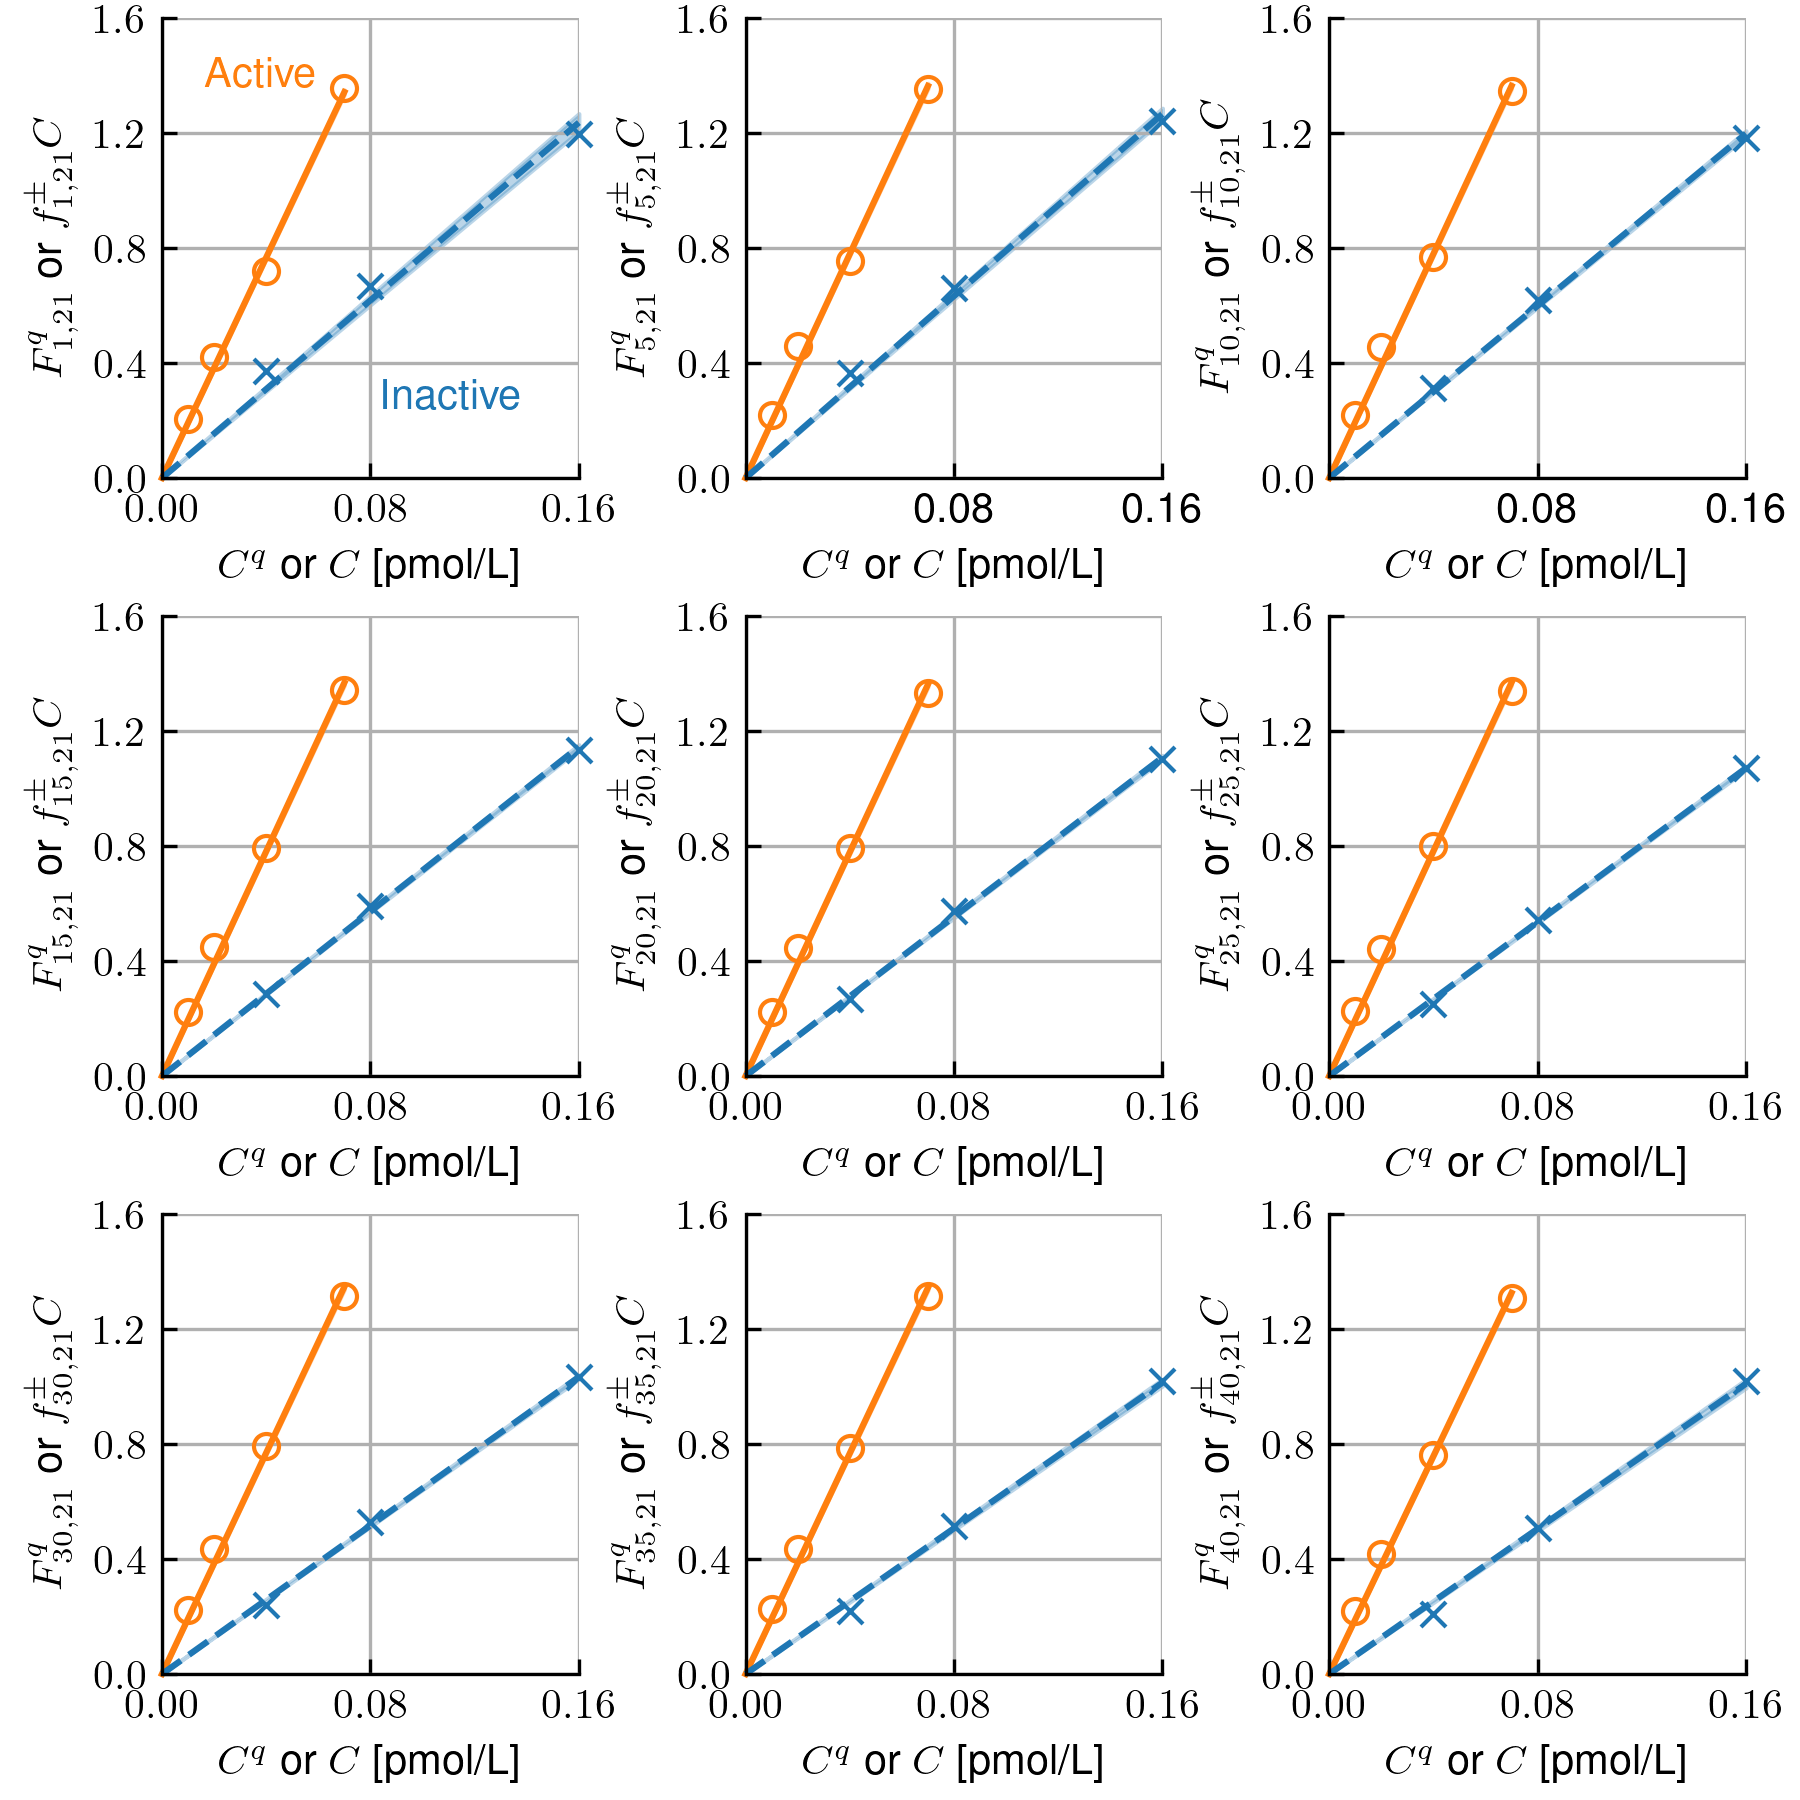
\includegraphics{si-figs/FigS21.png}
                    \caption{
                        As Figure~\ref{fig:S1} with well $w=21$ (or B9).
                    }
                \end{figure}
                \clearpage
    \begin{table}
        \caption{Molar Fluorescence Parameters for Well B9 ($w=21$)}
        \centering
        \begin{tabular}{c|ll|ll}
            Cycle & \multicolumn{2}{c|}{Inactive} & \multicolumn{2}{c}{Active} \\
            \hline
            $i$ & $f_{i,21}^{-}$ & $\sigma_{i,21}^{-}$ &  $f_{i,21}^{+}$ & $\sigma_{i,21}^{+}$ \\
            \hline
    1 & 7.73 & 0.064 & 19.18 & 0.036 \\
2 & 7.92 & 0.049 & 18.99 & 0.046 \\
3 & 8.03 & 0.045 & 19.27 & 0.046 \\
4 & 7.97 & 0.044 & 19.43 & 0.045 \\
5 & 7.91 & 0.043 & 19.48 & 0.045 \\
6 & 7.81 & 0.036 & 19.50 & 0.044 \\
7 & 7.73 & 0.031 & 19.50 & 0.043 \\
8 & 7.66 & 0.025 & 19.52 & 0.043 \\
9 & 7.57 & 0.023 & 19.50 & 0.042 \\
10 & 7.49 & 0.021 & 19.48 & 0.042 \\
11 & 7.42 & 0.018 & 19.53 & 0.041 \\
12 & 7.34 & 0.017 & 19.53 & 0.040 \\
13 & 7.29 & 0.014 & 19.57 & 0.041 \\
14 & 7.23 & 0.015 & 19.57 & 0.040 \\
15 & 7.15 & 0.016 & 19.54 & 0.040 \\
16 & 7.09 & 0.017 & 19.49 & 0.041 \\
17 & 7.05 & 0.016 & 19.49 & 0.040 \\
18 & 6.99 & 0.016 & 19.53 & 0.040 \\
19 & 6.95 & 0.016 & 19.51 & 0.040 \\
20 & 6.92 & 0.016 & 19.46 & 0.041 \\
21 & 6.88 & 0.016 & 19.44 & 0.043 \\
22 & 6.86 & 0.015 & 19.45 & 0.041 \\
23 & 6.80 & 0.017 & 19.48 & 0.042 \\
24 & 6.85 & 0.016 & 19.54 & 0.039 \\
25 & 6.69 & 0.013 & 19.55 & 0.041 \\
26 & 6.64 & 0.011 & 19.62 & 0.039 \\
27 & 6.60 & 0.013 & 19.39 & 0.044 \\
28 & 6.55 & 0.014 & 19.29 & 0.042 \\
29 & 6.51 & 0.016 & 19.26 & 0.042 \\
30 & 6.46 & 0.015 & 19.24 & 0.042 \\
31 & 6.43 & 0.016 & 19.26 & 0.043 \\
32 & 6.41 & 0.017 & 19.16 & 0.039 \\
33 & 6.38 & 0.015 & 19.27 & 0.037 \\
34 & 6.37 & 0.024 & 19.26 & 0.038 \\
35 & 6.34 & 0.024 & 19.19 & 0.040 \\
36 & 6.33 & 0.026 & 19.15 & 0.036 \\
37 & 6.32 & 0.028 & 19.30 & 0.030 \\
38 & 6.30 & 0.029 & 19.31 & 0.032 \\
39 & 6.21 & 0.028 & 19.03 & 0.028 \\
40 & 6.31 & 0.031 & 18.94 & 0.030 \\
41 & 6.23 & 0.032 & 18.91 & 0.032 \\
42 & 6.20 & 0.031 & 18.89 & 0.033 \\
43 & 6.25 & 0.035 & 18.88 & 0.035 \\
44 & 6.16 & 0.033 & 18.89 & 0.035 \\
45 & 6.14 & 0.040 & 18.90 & 0.035 \\
               \hline
        \end{tabular}
    \end{table}
    \clearpage

                \begin{figure}
                    \centering
                    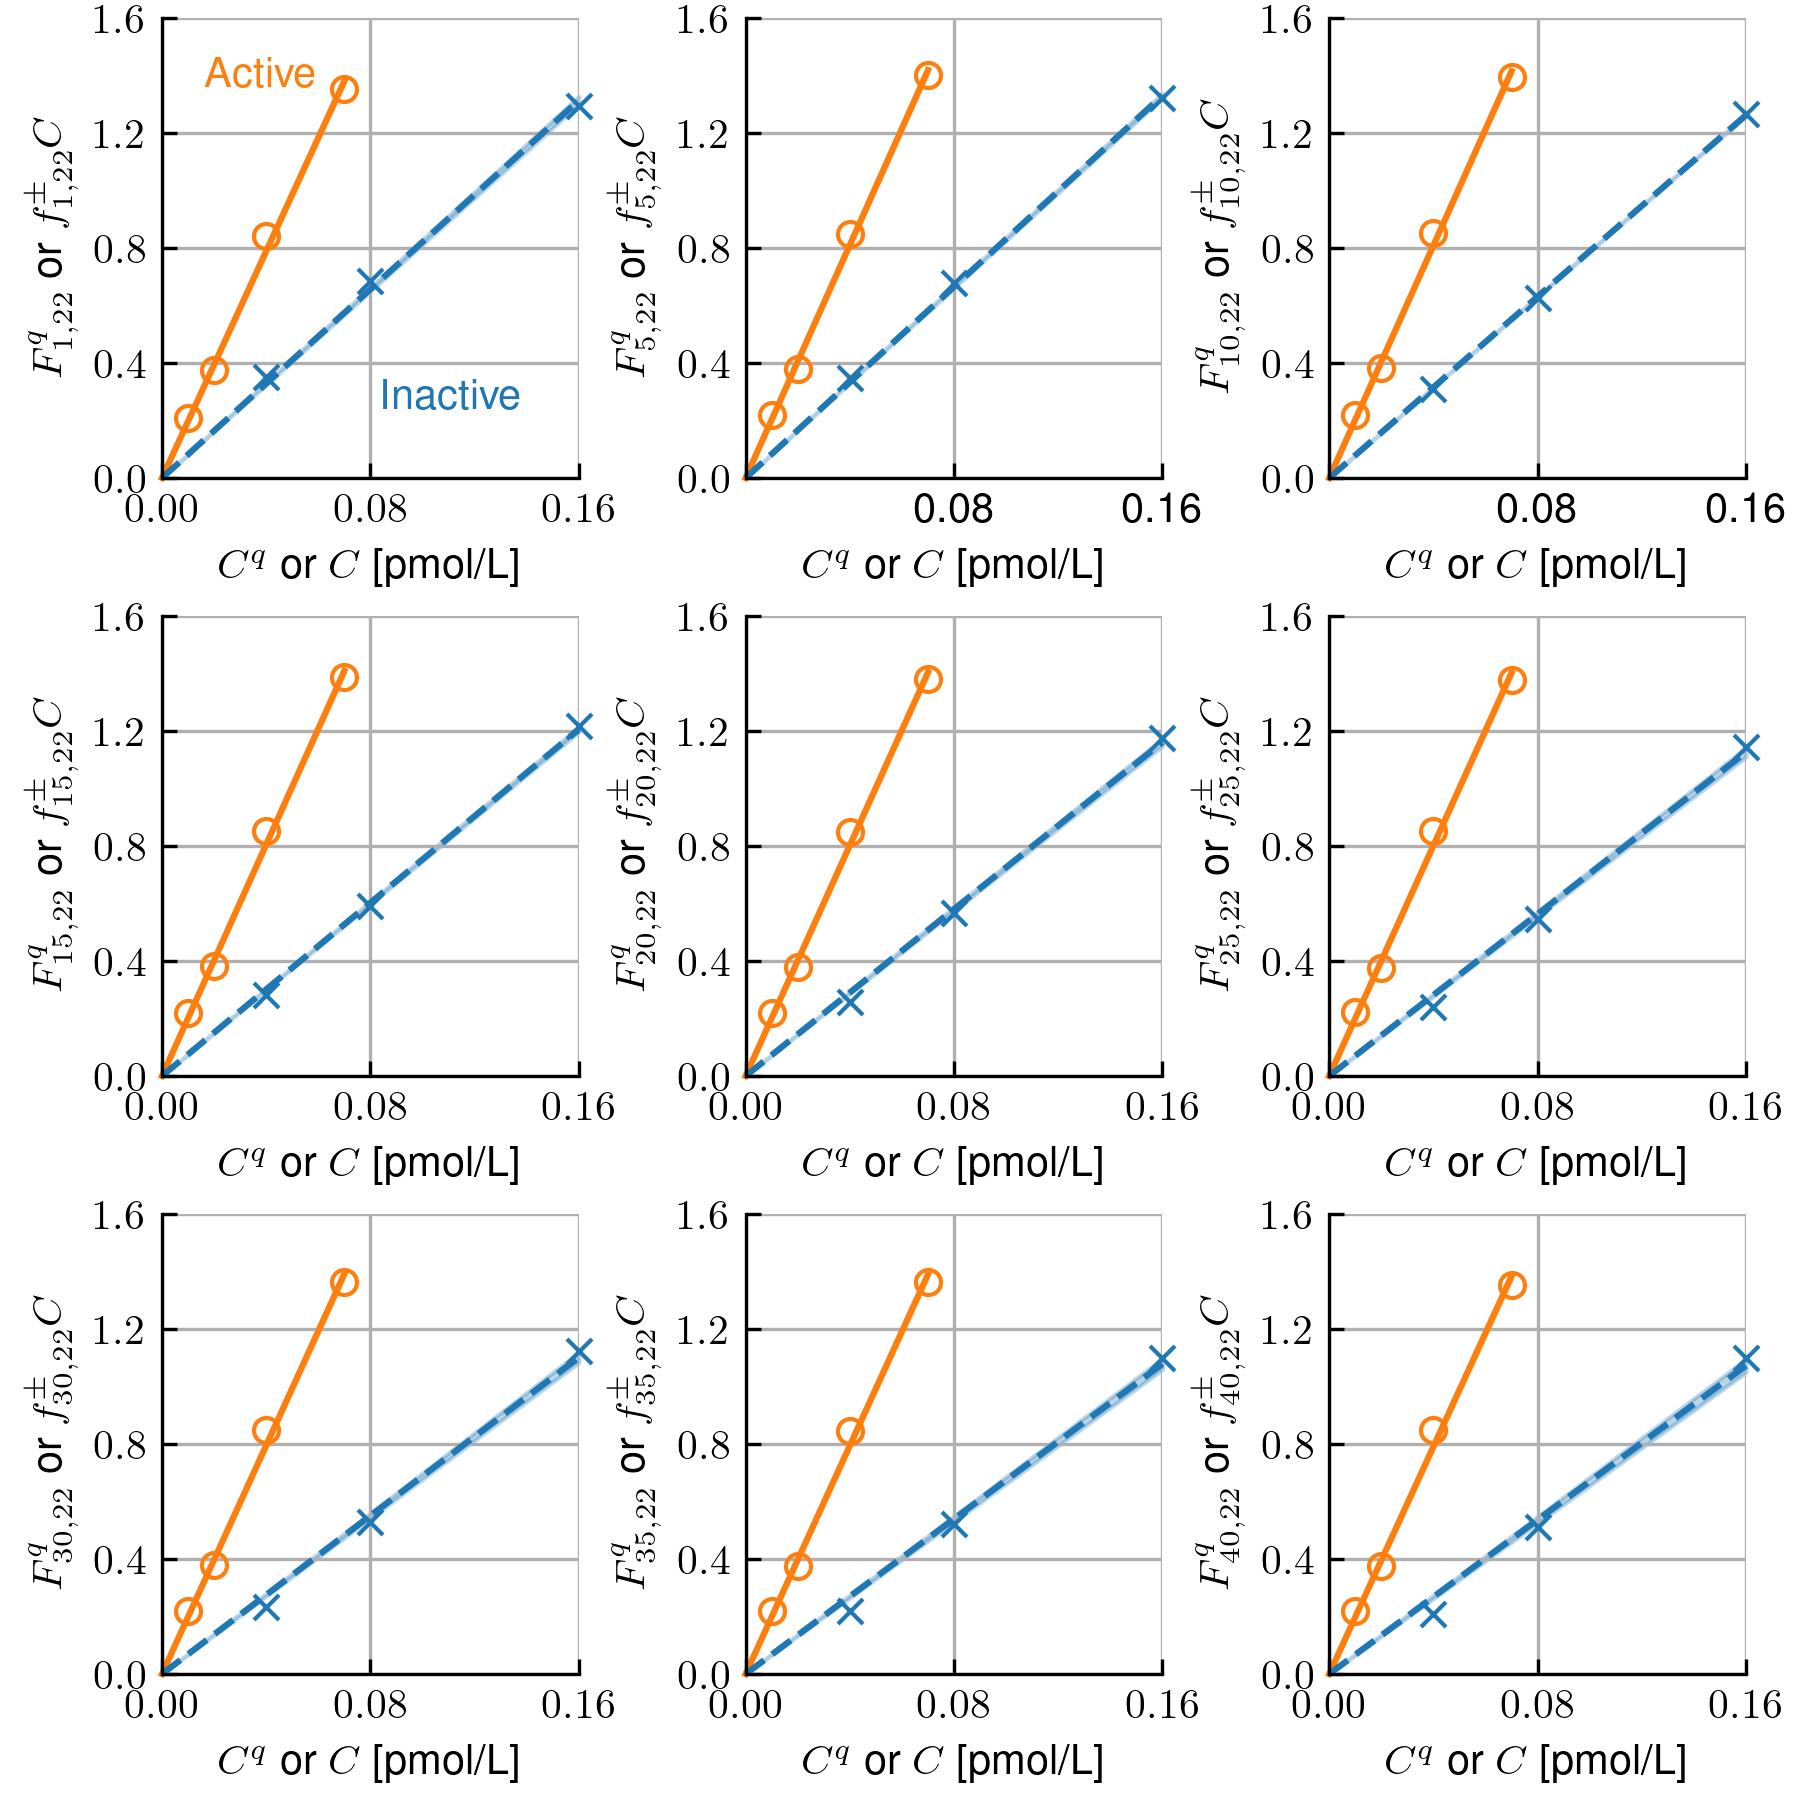
\includegraphics{si-figs/FigS22.png}
                    \caption{
                        As Figure~\ref{fig:S1} with well $w=22$ (or B10).
                    }
                \end{figure}
                \clearpage
    \begin{table}
        \caption{Molar Fluorescence Parameters for Well B10 ($w=22$)}
        \centering
        \begin{tabular}{c|ll|ll}
            Cycle & \multicolumn{2}{c|}{Inactive} & \multicolumn{2}{c}{Active} \\
            \hline
            $i$ & $f_{i,22}^{-}$ & $\sigma_{i,22}^{-}$ &  $f_{i,22}^{+}$ & $\sigma_{i,22}^{+}$ \\
            \hline
    1 & 8.21 & 0.029 & 19.73 & 0.036 \\
2 & 8.31 & 0.025 & 19.79 & 0.028 \\
3 & 8.44 & 0.021 & 20.08 & 0.026 \\
4 & 8.40 & 0.022 & 20.24 & 0.028 \\
5 & 8.31 & 0.016 & 20.26 & 0.031 \\
6 & 8.248 & 0.0091 & 20.24 & 0.031 \\
7 & 8.142 & 0.0051 & 20.26 & 0.031 \\
8 & 8.062 & 0.0011 & 20.24 & 0.032 \\
9 & 7.976 & 0.0025 & 20.26 & 0.032 \\
10 & 7.888 & 0.0055 & 20.22 & 0.032 \\
11 & 7.807 & 0.0083 & 20.21 & 0.032 \\
12 & 7.74 & 0.011 & 20.21 & 0.033 \\
13 & 7.66 & 0.013 & 20.16 & 0.033 \\
14 & 7.60 & 0.017 & 20.15 & 0.034 \\
15 & 7.53 & 0.018 & 20.14 & 0.034 \\
16 & 7.47 & 0.019 & 20.09 & 0.035 \\
17 & 7.42 & 0.022 & 20.16 & 0.033 \\
18 & 7.36 & 0.024 & 20.06 & 0.035 \\
19 & 7.32 & 0.026 & 20.11 & 0.034 \\
20 & 7.26 & 0.027 & 20.05 & 0.035 \\
21 & 7.20 & 0.028 & 20.04 & 0.035 \\
22 & 7.17 & 0.029 & 20.02 & 0.035 \\
23 & 7.12 & 0.031 & 20.00 & 0.038 \\
24 & 7.09 & 0.033 & 20.09 & 0.033 \\
25 & 7.04 & 0.033 & 20.03 & 0.037 \\
26 & 7.00 & 0.035 & 19.96 & 0.036 \\
27 & 6.98 & 0.036 & 19.99 & 0.037 \\
28 & 6.94 & 0.035 & 19.93 & 0.039 \\
29 & 6.91 & 0.035 & 19.89 & 0.038 \\
30 & 6.88 & 0.037 & 19.89 & 0.038 \\
31 & 6.91 & 0.039 & 20.00 & 0.034 \\
32 & 6.87 & 0.037 & 19.93 & 0.036 \\
33 & 6.83 & 0.036 & 19.88 & 0.037 \\
34 & 6.80 & 0.037 & 19.95 & 0.037 \\
35 & 6.74 & 0.040 & 19.86 & 0.038 \\
36 & 6.71 & 0.042 & 19.78 & 0.035 \\
37 & 6.65 & 0.039 & 19.83 & 0.042 \\
38 & 6.62 & 0.036 & 19.78 & 0.041 \\
39 & 6.68 & 0.046 & 19.74 & 0.038 \\
40 & 6.70 & 0.048 & 19.77 & 0.041 \\
41 & 6.71 & 0.054 & 19.97 & 0.035 \\
42 & 6.68 & 0.053 & 19.95 & 0.035 \\
43 & 6.64 & 0.051 & 19.85 & 0.033 \\
44 & 6.66 & 0.053 & 19.86 & 0.037 \\
45 & 6.67 & 0.053 & 19.79 & 0.038 \\
               \hline
        \end{tabular}
    \end{table}
    \clearpage

                \begin{figure}
                    \centering
                    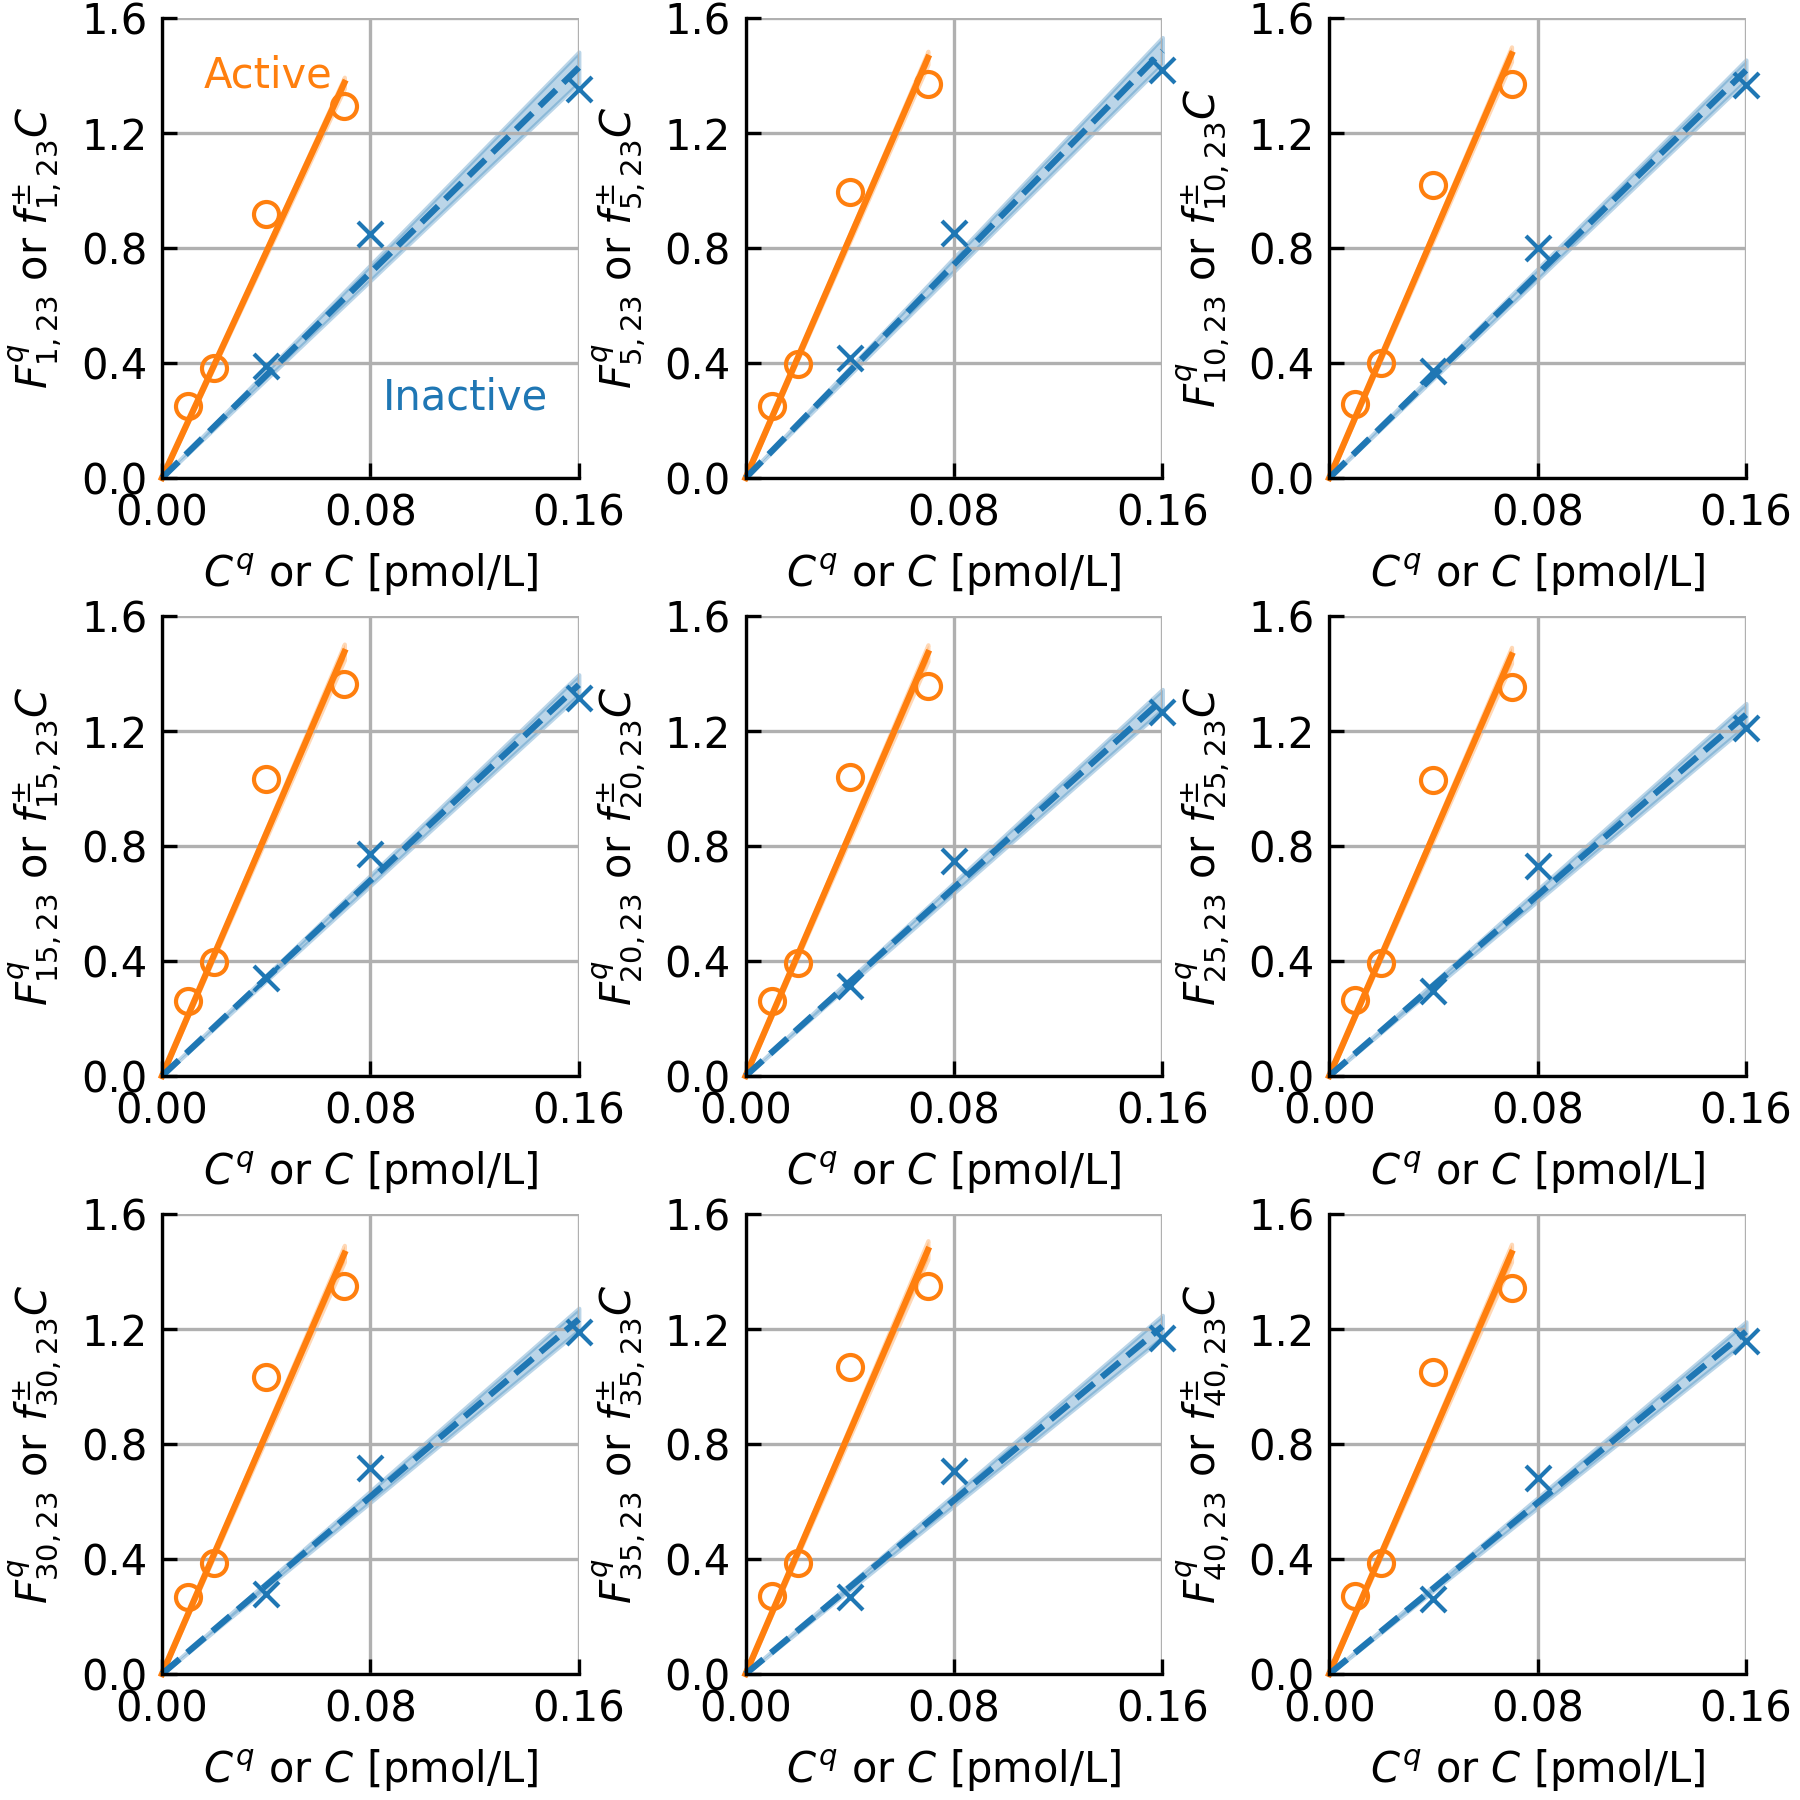
\includegraphics{si-figs/FigS23.png}
                    \caption{
                        As Figure~\ref{fig:S1} with well $w=23$ (or B11).
                    }
                \end{figure}
                \clearpage
    \begin{table}
        \caption{Molar Fluorescence Parameters for Well B11 ($w=23$)}
        \centering
        \begin{tabular}{c|ll|ll}
            Cycle & \multicolumn{2}{c|}{Inactive} & \multicolumn{2}{c}{Active} \\
            \hline
            $i$ & $f_{i,23}^{-}$ & $\sigma_{i,23}^{-}$ &  $f_{i,23}^{+}$ & $\sigma_{i,23}^{+}$ \\
            \hline
    1 & 8.9 & 0.11 & 19.63 & 0.094 \\
2 & 9.2 & 0.10 & 20.15 & 0.099 \\
3 & 9.37 & 0.100 & 20.5 & 0.11 \\
4 & 9.36 & 0.100 & 20.7 & 0.11 \\
5 & 9.28 & 0.097 & 20.9 & 0.11 \\
6 & 9.22 & 0.090 & 20.9 & 0.11 \\
7 & 9.13 & 0.084 & 21.0 & 0.12 \\
8 & 9.02 & 0.082 & 21.0 & 0.12 \\
9 & 8.94 & 0.077 & 21.1 & 0.12 \\
10 & 8.86 & 0.075 & 21.1 & 0.12 \\
11 & 8.77 & 0.076 & 21.1 & 0.12 \\
12 & 8.70 & 0.075 & 21.1 & 0.13 \\
13 & 8.64 & 0.075 & 21.1 & 0.13 \\
14 & 8.57 & 0.074 & 21.1 & 0.13 \\
15 & 8.51 & 0.073 & 21.1 & 0.13 \\
16 & 8.44 & 0.072 & 21.0 & 0.13 \\
17 & 8.36 & 0.073 & 21.0 & 0.13 \\
18 & 8.30 & 0.074 & 21.0 & 0.13 \\
19 & 8.25 & 0.072 & 21.0 & 0.13 \\
20 & 8.18 & 0.074 & 21.0 & 0.14 \\
21 & 8.15 & 0.073 & 21.0 & 0.14 \\
22 & 8.01 & 0.080 & 21.0 & 0.14 \\
23 & 7.98 & 0.078 & 21.0 & 0.14 \\
24 & 7.92 & 0.080 & 20.9 & 0.13 \\
25 & 7.86 & 0.081 & 20.9 & 0.13 \\
26 & 7.82 & 0.081 & 20.9 & 0.14 \\
27 & 7.78 & 0.081 & 20.9 & 0.14 \\
28 & 7.76 & 0.080 & 20.8 & 0.13 \\
29 & 7.72 & 0.081 & 20.9 & 0.14 \\
30 & 7.71 & 0.080 & 20.9 & 0.14 \\
31 & 7.63 & 0.084 & 21.0 & 0.14 \\
32 & 7.60 & 0.085 & 20.9 & 0.14 \\
33 & 7.56 & 0.084 & 21.0 & 0.15 \\
34 & 7.54 & 0.083 & 21.0 & 0.15 \\
35 & 7.56 & 0.080 & 21.1 & 0.15 \\
36 & 7.55 & 0.081 & 21.0 & 0.16 \\
37 & 7.56 & 0.078 & 21.0 & 0.16 \\
38 & 7.52 & 0.070 & 21.1 & 0.16 \\
39 & 7.50 & 0.070 & 21.1 & 0.16 \\
40 & 7.44 & 0.071 & 20.9 & 0.15 \\
41 & 7.36 & 0.074 & 20.9 & 0.15 \\
42 & 7.34 & 0.074 & 20.9 & 0.15 \\
43 & 7.35 & 0.073 & 20.9 & 0.15 \\
44 & 7.38 & 0.070 & 20.9 & 0.15 \\
45 & 7.31 & 0.073 & 20.9 & 0.15 \\
               \hline
        \end{tabular}
    \end{table}
    \clearpage

                \begin{figure}
                    \centering
                    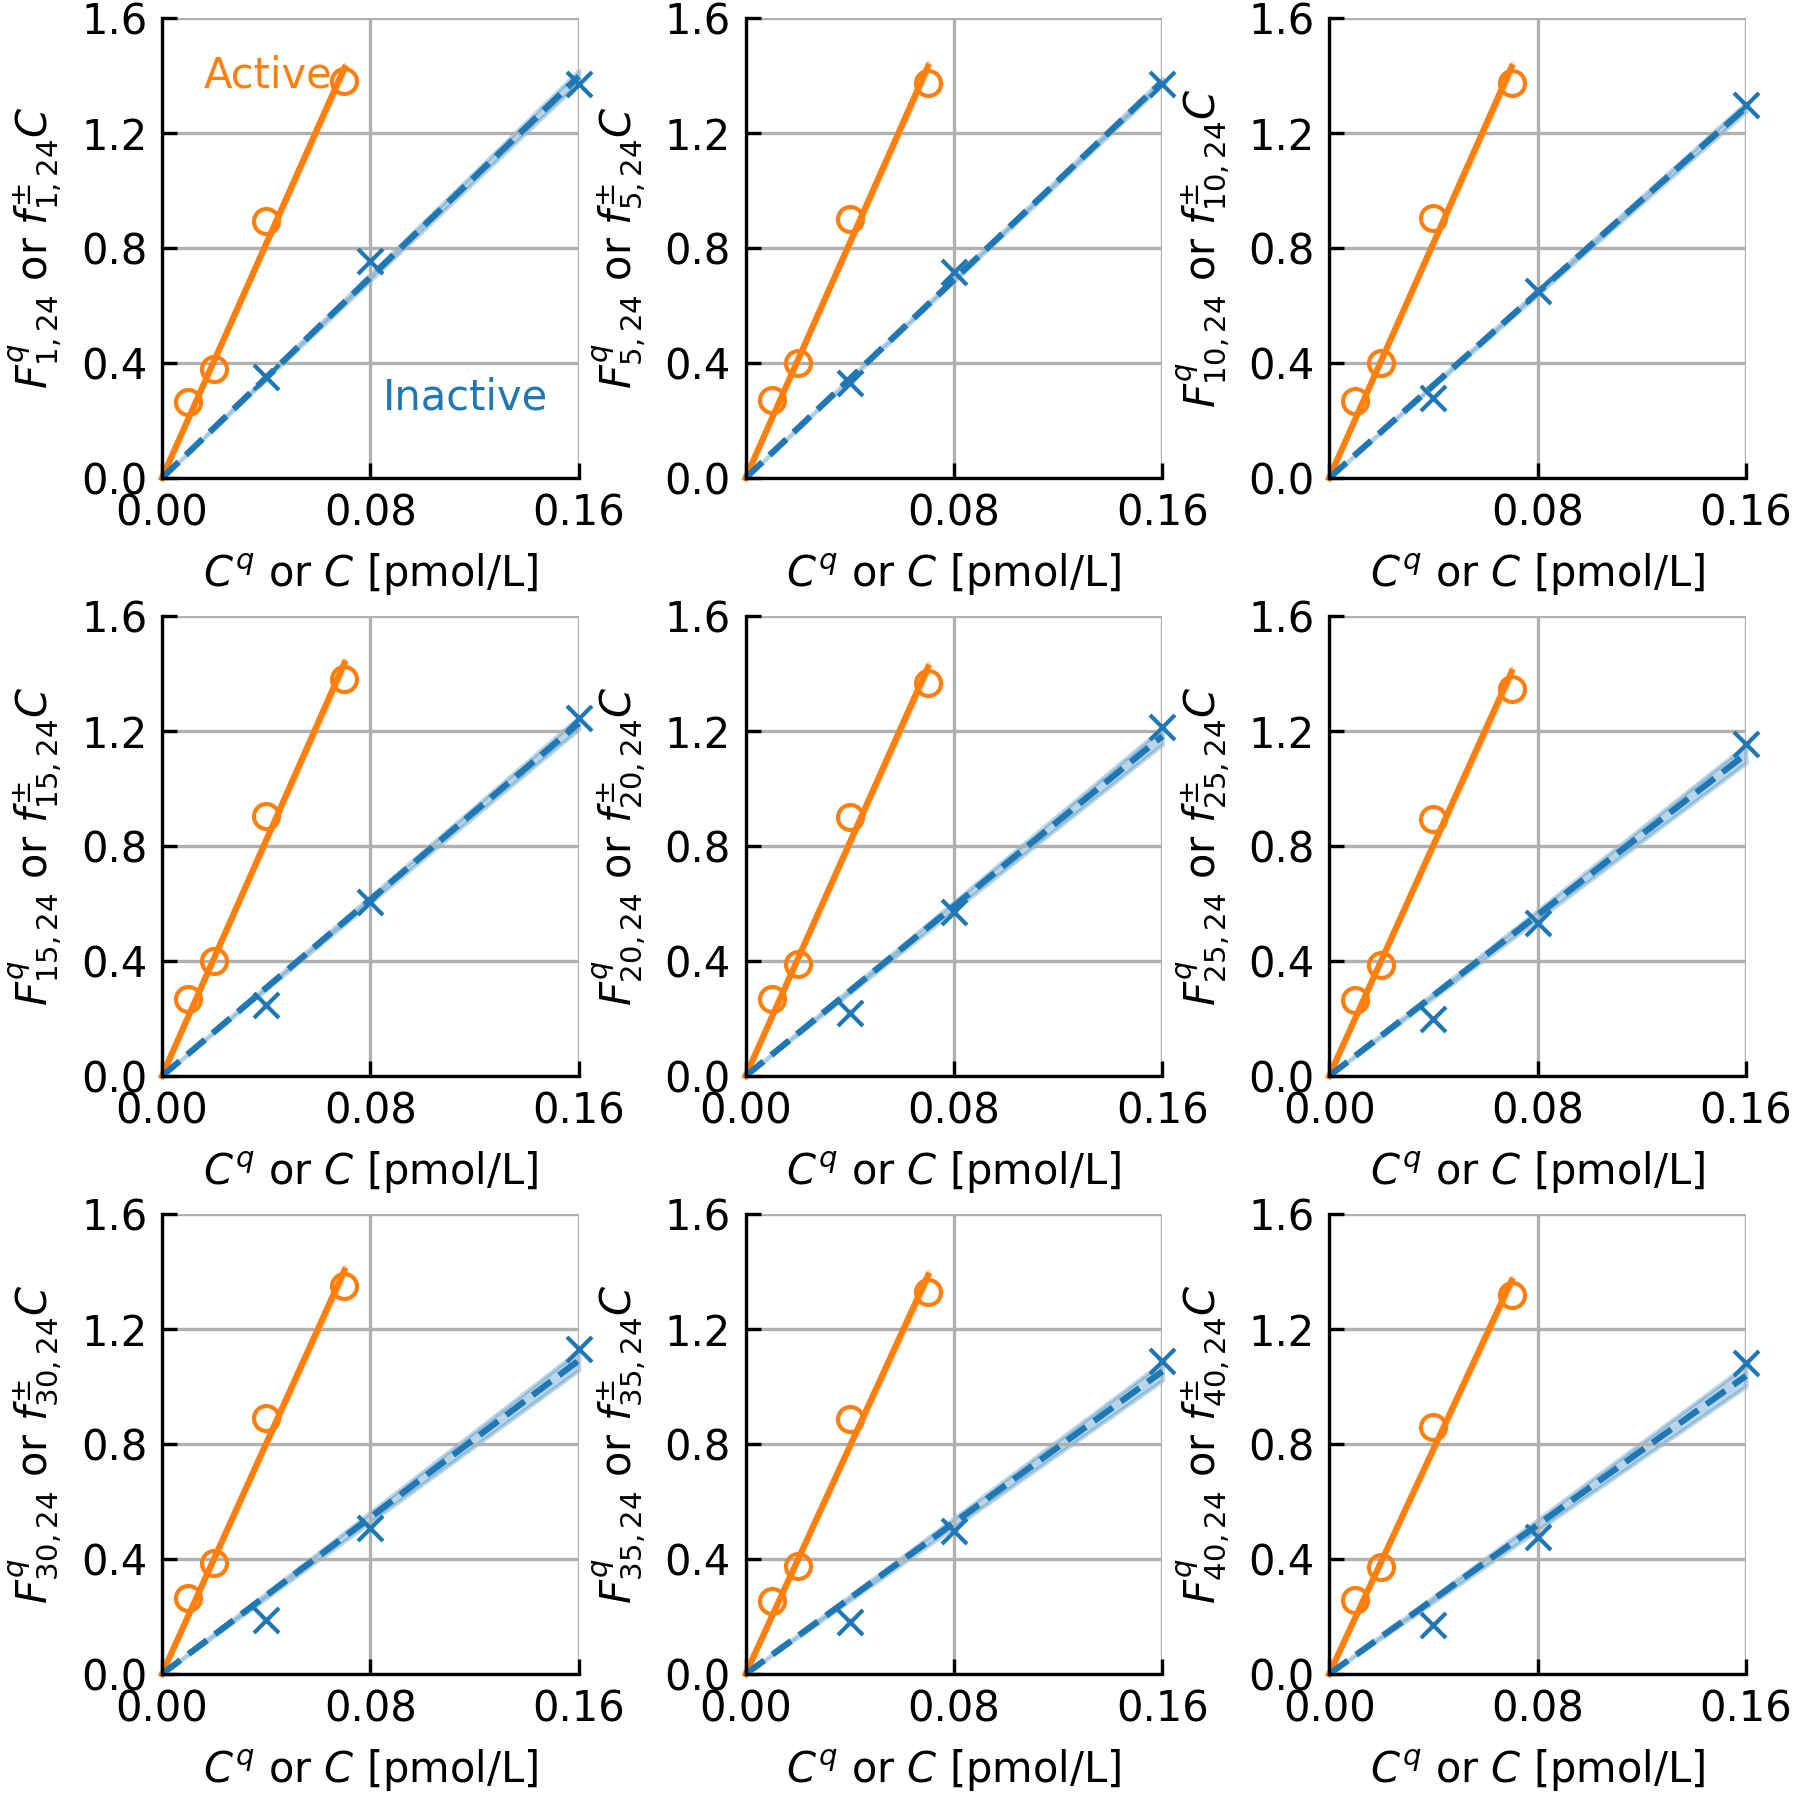
\includegraphics{si-figs/FigS24.png}
                    \caption{
                        As Figure~\ref{fig:S1} with well $w=24$ (or B12).
                    }
                \end{figure}
                \clearpage
    \begin{table}
        \caption{Molar Fluorescence Parameters for Well B12 ($w=24$)}
        \centering
        \begin{tabular}{c|ll|ll}
            Cycle & \multicolumn{2}{c|}{Inactive} & \multicolumn{2}{c}{Active} \\
            \hline
            $i$ & $f_{i,24}^{-}$ & $\sigma_{i,24}^{-}$ &  $f_{i,24}^{+}$ & $\sigma_{i,24}^{+}$ \\
            \hline
    1 & 8.73 & 0.044 & 20.37 & 0.066 \\
2 & 8.80 & 0.041 & 20.13 & 0.066 \\
3 & 8.85 & 0.033 & 20.32 & 0.070 \\
4 & 8.76 & 0.027 & 20.40 & 0.070 \\
5 & 8.62 & 0.022 & 20.45 & 0.071 \\
6 & 8.50 & 0.021 & 20.44 & 0.071 \\
7 & 8.38 & 0.023 & 20.47 & 0.071 \\
8 & 8.27 & 0.025 & 20.44 & 0.071 \\
9 & 8.17 & 0.029 & 20.42 & 0.072 \\
10 & 8.06 & 0.032 & 20.42 & 0.071 \\
11 & 8.01 & 0.036 & 20.42 & 0.071 \\
12 & 7.90 & 0.039 & 20.51 & 0.068 \\
13 & 7.82 & 0.042 & 20.35 & 0.073 \\
14 & 7.75 & 0.044 & 20.37 & 0.071 \\
15 & 7.67 & 0.044 & 20.51 & 0.068 \\
16 & 7.63 & 0.050 & 20.38 & 0.072 \\
17 & 7.60 & 0.054 & 20.28 & 0.071 \\
18 & 7.49 & 0.055 & 20.30 & 0.071 \\
19 & 7.42 & 0.056 & 20.29 & 0.070 \\
20 & 7.39 & 0.060 & 20.30 & 0.071 \\
21 & 7.28 & 0.060 & 20.13 & 0.073 \\
22 & 7.18 & 0.059 & 20.12 & 0.073 \\
23 & 7.12 & 0.061 & 20.10 & 0.073 \\
24 & 7.06 & 0.064 & 20.07 & 0.074 \\
25 & 7.00 & 0.065 & 20.07 & 0.073 \\
26 & 6.94 & 0.066 & 20.13 & 0.077 \\
27 & 6.87 & 0.066 & 20.08 & 0.070 \\
28 & 6.86 & 0.068 & 20.15 & 0.069 \\
29 & 6.81 & 0.065 & 20.09 & 0.070 \\
30 & 6.82 & 0.071 & 20.05 & 0.070 \\
31 & 6.72 & 0.068 & 20.05 & 0.070 \\
32 & 6.69 & 0.066 & 20.08 & 0.069 \\
33 & 6.66 & 0.067 & 19.91 & 0.073 \\
34 & 6.63 & 0.068 & 19.81 & 0.076 \\
35 & 6.58 & 0.066 & 19.80 & 0.073 \\
36 & 6.52 & 0.068 & 19.76 & 0.073 \\
37 & 6.50 & 0.067 & 19.77 & 0.075 \\
38 & 6.51 & 0.070 & 19.69 & 0.065 \\
39 & 6.46 & 0.072 & 19.58 & 0.063 \\
40 & 6.48 & 0.076 & 19.54 & 0.064 \\
41 & 6.49 & 0.080 & 19.54 & 0.065 \\
42 & 6.45 & 0.083 & 19.36 & 0.070 \\
43 & 6.47 & 0.084 & 19.37 & 0.069 \\
44 & 6.44 & 0.085 & 19.38 & 0.070 \\
45 & 6.37 & 0.084 & 19.35 & 0.071 \\
               \hline
        \end{tabular}
    \end{table}
    \clearpage

                \begin{figure}
                    \centering
                    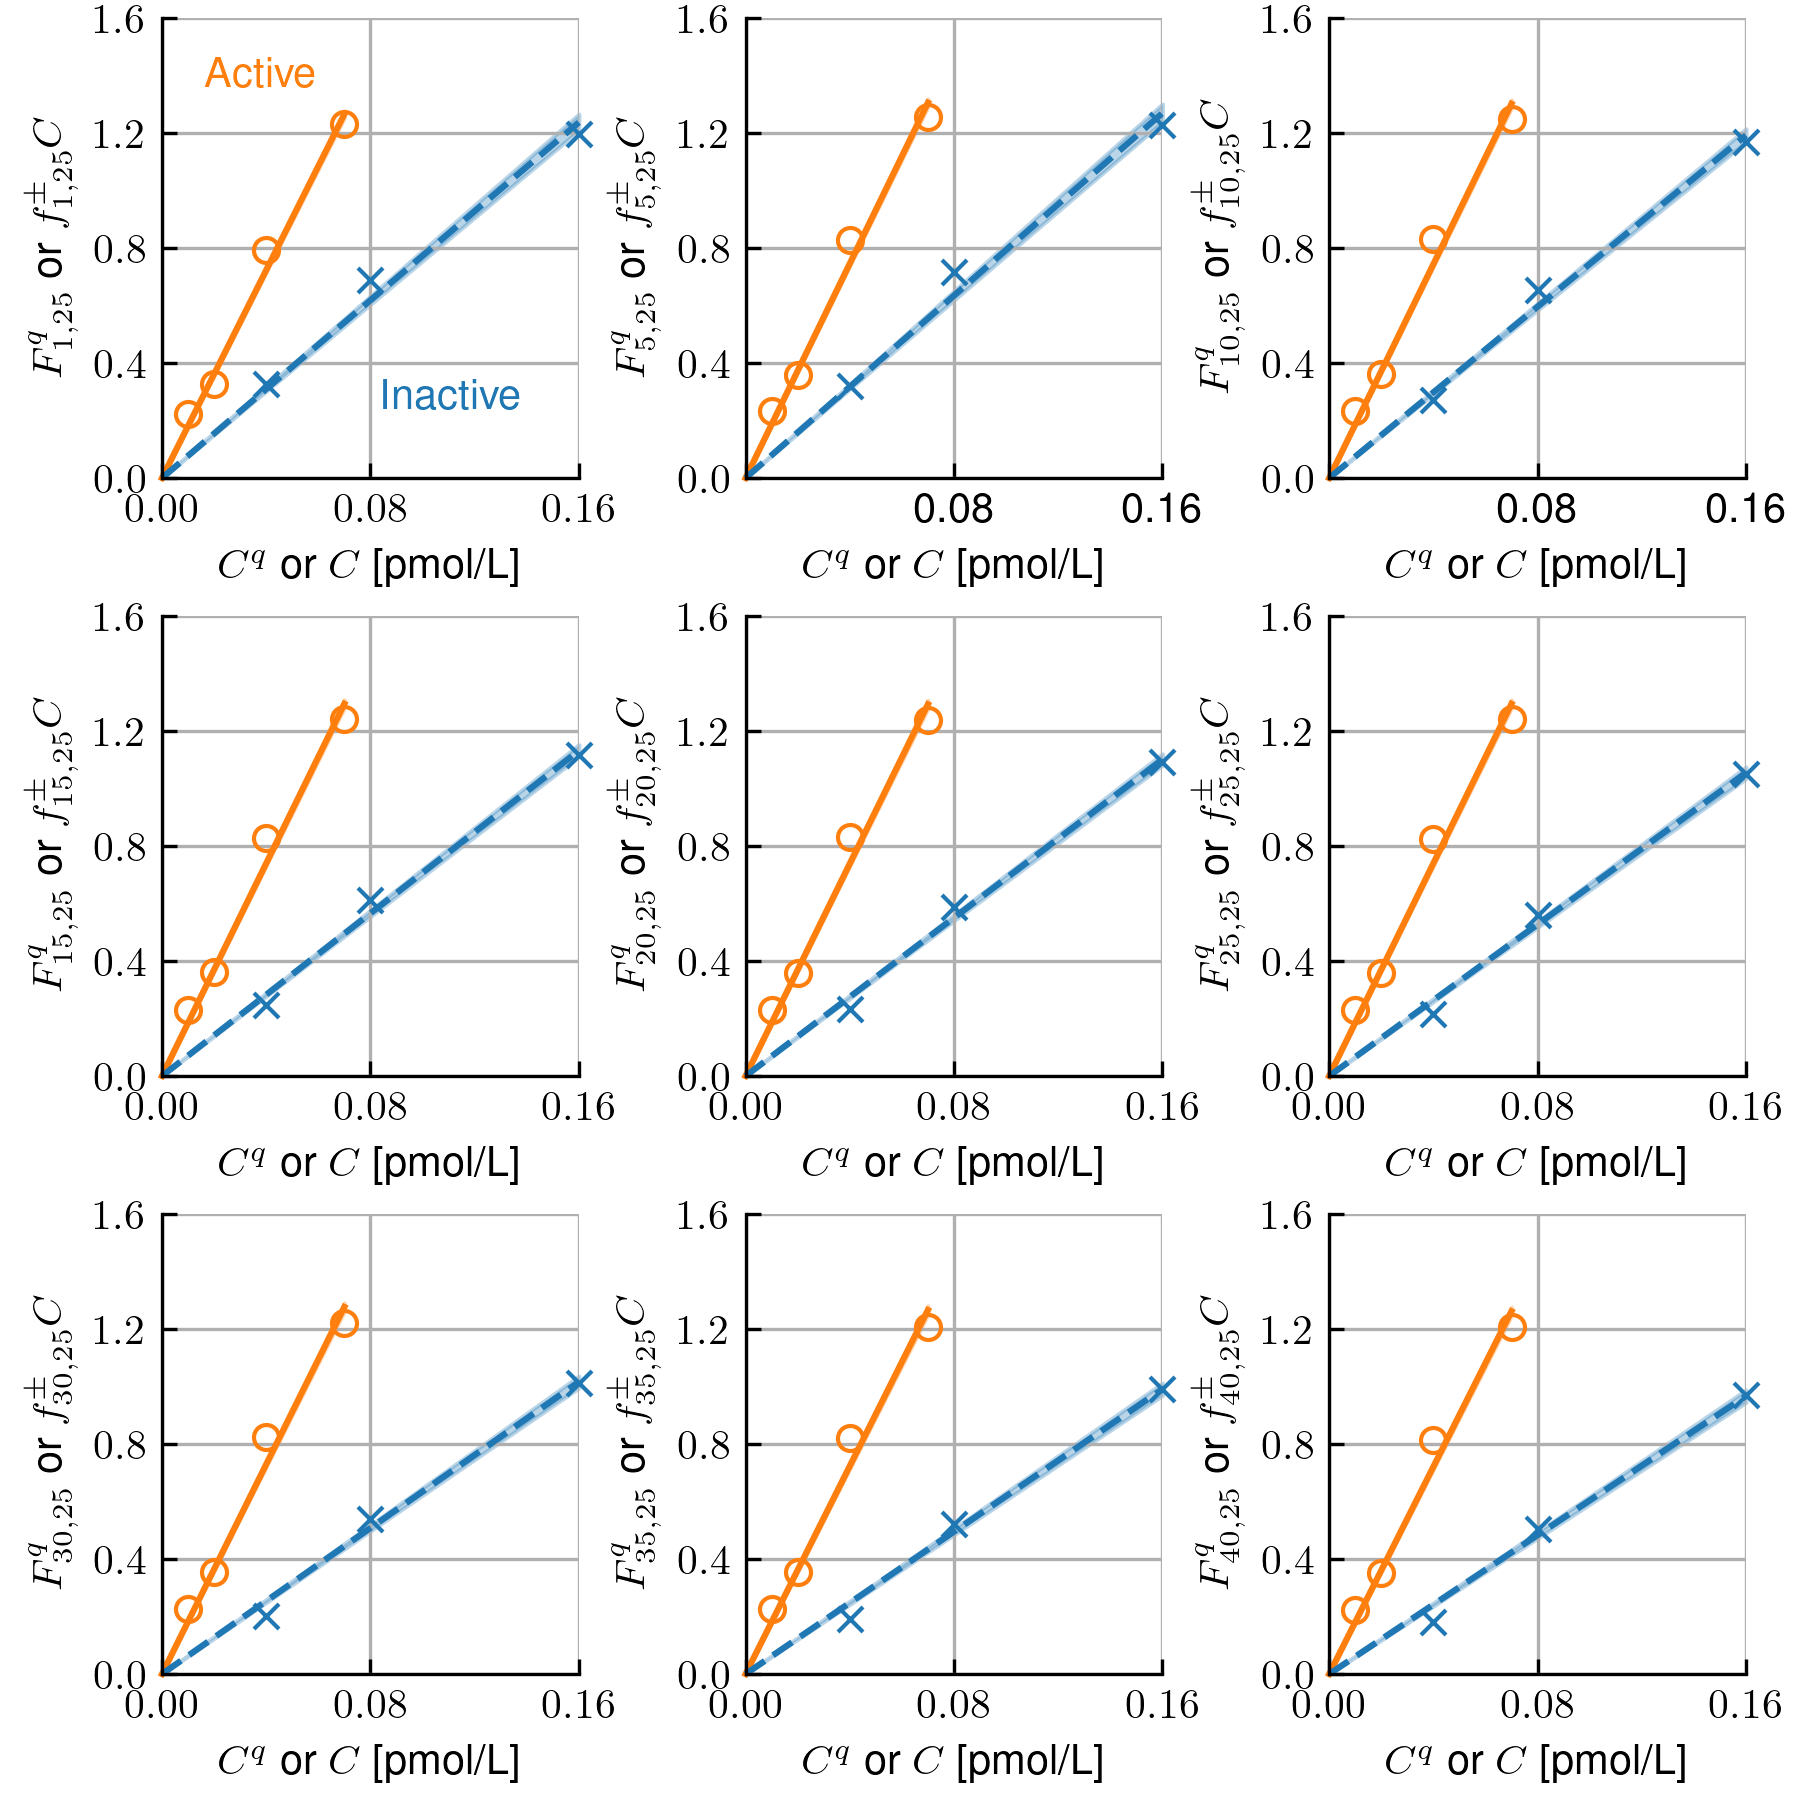
\includegraphics{si-figs/FigS25.png}
                    \caption{
                        As Figure~\ref{fig:S1} with well $w=25$ (or C1).
                    }
                \end{figure}
                \clearpage
    \begin{table}
        \caption{Molar Fluorescence Parameters for Well C1 ($w=25$)}
        \centering
        \begin{tabular}{c|ll|ll}
            Cycle & \multicolumn{2}{c|}{Inactive} & \multicolumn{2}{c}{Active} \\
            \hline
            $i$ & $f_{i,25}^{-}$ & $\sigma_{i,25}^{-}$ &  $f_{i,25}^{+}$ & $\sigma_{i,25}^{+}$ \\
            \hline
    1 & 7.73 & 0.059 & 18.08 & 0.055 \\
2 & 8.04 & 0.071 & 18.30 & 0.053 \\
3 & 8.14 & 0.070 & 18.55 & 0.055 \\
4 & 8.06 & 0.068 & 18.62 & 0.058 \\
5 & 7.93 & 0.065 & 18.65 & 0.061 \\
6 & 7.82 & 0.061 & 18.64 & 0.062 \\
7 & 7.72 & 0.056 & 18.64 & 0.062 \\
8 & 7.61 & 0.053 & 18.66 & 0.062 \\
9 & 7.52 & 0.050 & 18.63 & 0.063 \\
10 & 7.45 & 0.047 & 18.59 & 0.064 \\
11 & 7.36 & 0.047 & 18.57 & 0.065 \\
12 & 7.30 & 0.046 & 18.54 & 0.064 \\
13 & 7.25 & 0.046 & 18.56 & 0.063 \\
14 & 7.15 & 0.046 & 18.50 & 0.065 \\
15 & 7.07 & 0.043 & 18.50 & 0.065 \\
16 & 7.02 & 0.043 & 18.48 & 0.066 \\
17 & 6.98 & 0.040 & 18.50 & 0.067 \\
18 & 6.93 & 0.040 & 18.50 & 0.068 \\
19 & 6.88 & 0.040 & 18.47 & 0.066 \\
20 & 6.88 & 0.041 & 18.47 & 0.067 \\
21 & 6.84 & 0.041 & 18.68 & 0.062 \\
22 & 6.79 & 0.040 & 18.50 & 0.064 \\
23 & 6.77 & 0.040 & 18.46 & 0.065 \\
24 & 6.70 & 0.040 & 18.40 & 0.068 \\
25 & 6.59 & 0.042 & 18.49 & 0.064 \\
26 & 6.56 & 0.042 & 18.34 & 0.067 \\
27 & 6.51 & 0.043 & 18.28 & 0.069 \\
28 & 6.44 & 0.042 & 18.27 & 0.069 \\
29 & 6.38 & 0.043 & 18.26 & 0.068 \\
30 & 6.35 & 0.042 & 18.23 & 0.068 \\
31 & 6.32 & 0.045 & 18.28 & 0.073 \\
32 & 6.30 & 0.044 & 18.15 & 0.070 \\
33 & 6.26 & 0.044 & 18.13 & 0.070 \\
34 & 6.25 & 0.044 & 18.10 & 0.070 \\
35 & 6.19 & 0.044 & 18.08 & 0.070 \\
36 & 6.14 & 0.045 & 18.09 & 0.069 \\
37 & 6.08 & 0.046 & 18.07 & 0.068 \\
38 & 6.06 & 0.046 & 18.04 & 0.068 \\
39 & 6.05 & 0.045 & 18.02 & 0.068 \\
40 & 6.04 & 0.045 & 18.02 & 0.067 \\
41 & 5.98 & 0.045 & 17.83 & 0.073 \\
42 & 5.95 & 0.048 & 17.83 & 0.071 \\
43 & 5.90 & 0.047 & 17.83 & 0.070 \\
44 & 5.89 & 0.048 & 17.72 & 0.072 \\
45 & 5.87 & 0.049 & 17.70 & 0.072 \\
               \hline
        \end{tabular}
    \end{table}
    \clearpage

                \begin{figure}
                    \centering
                    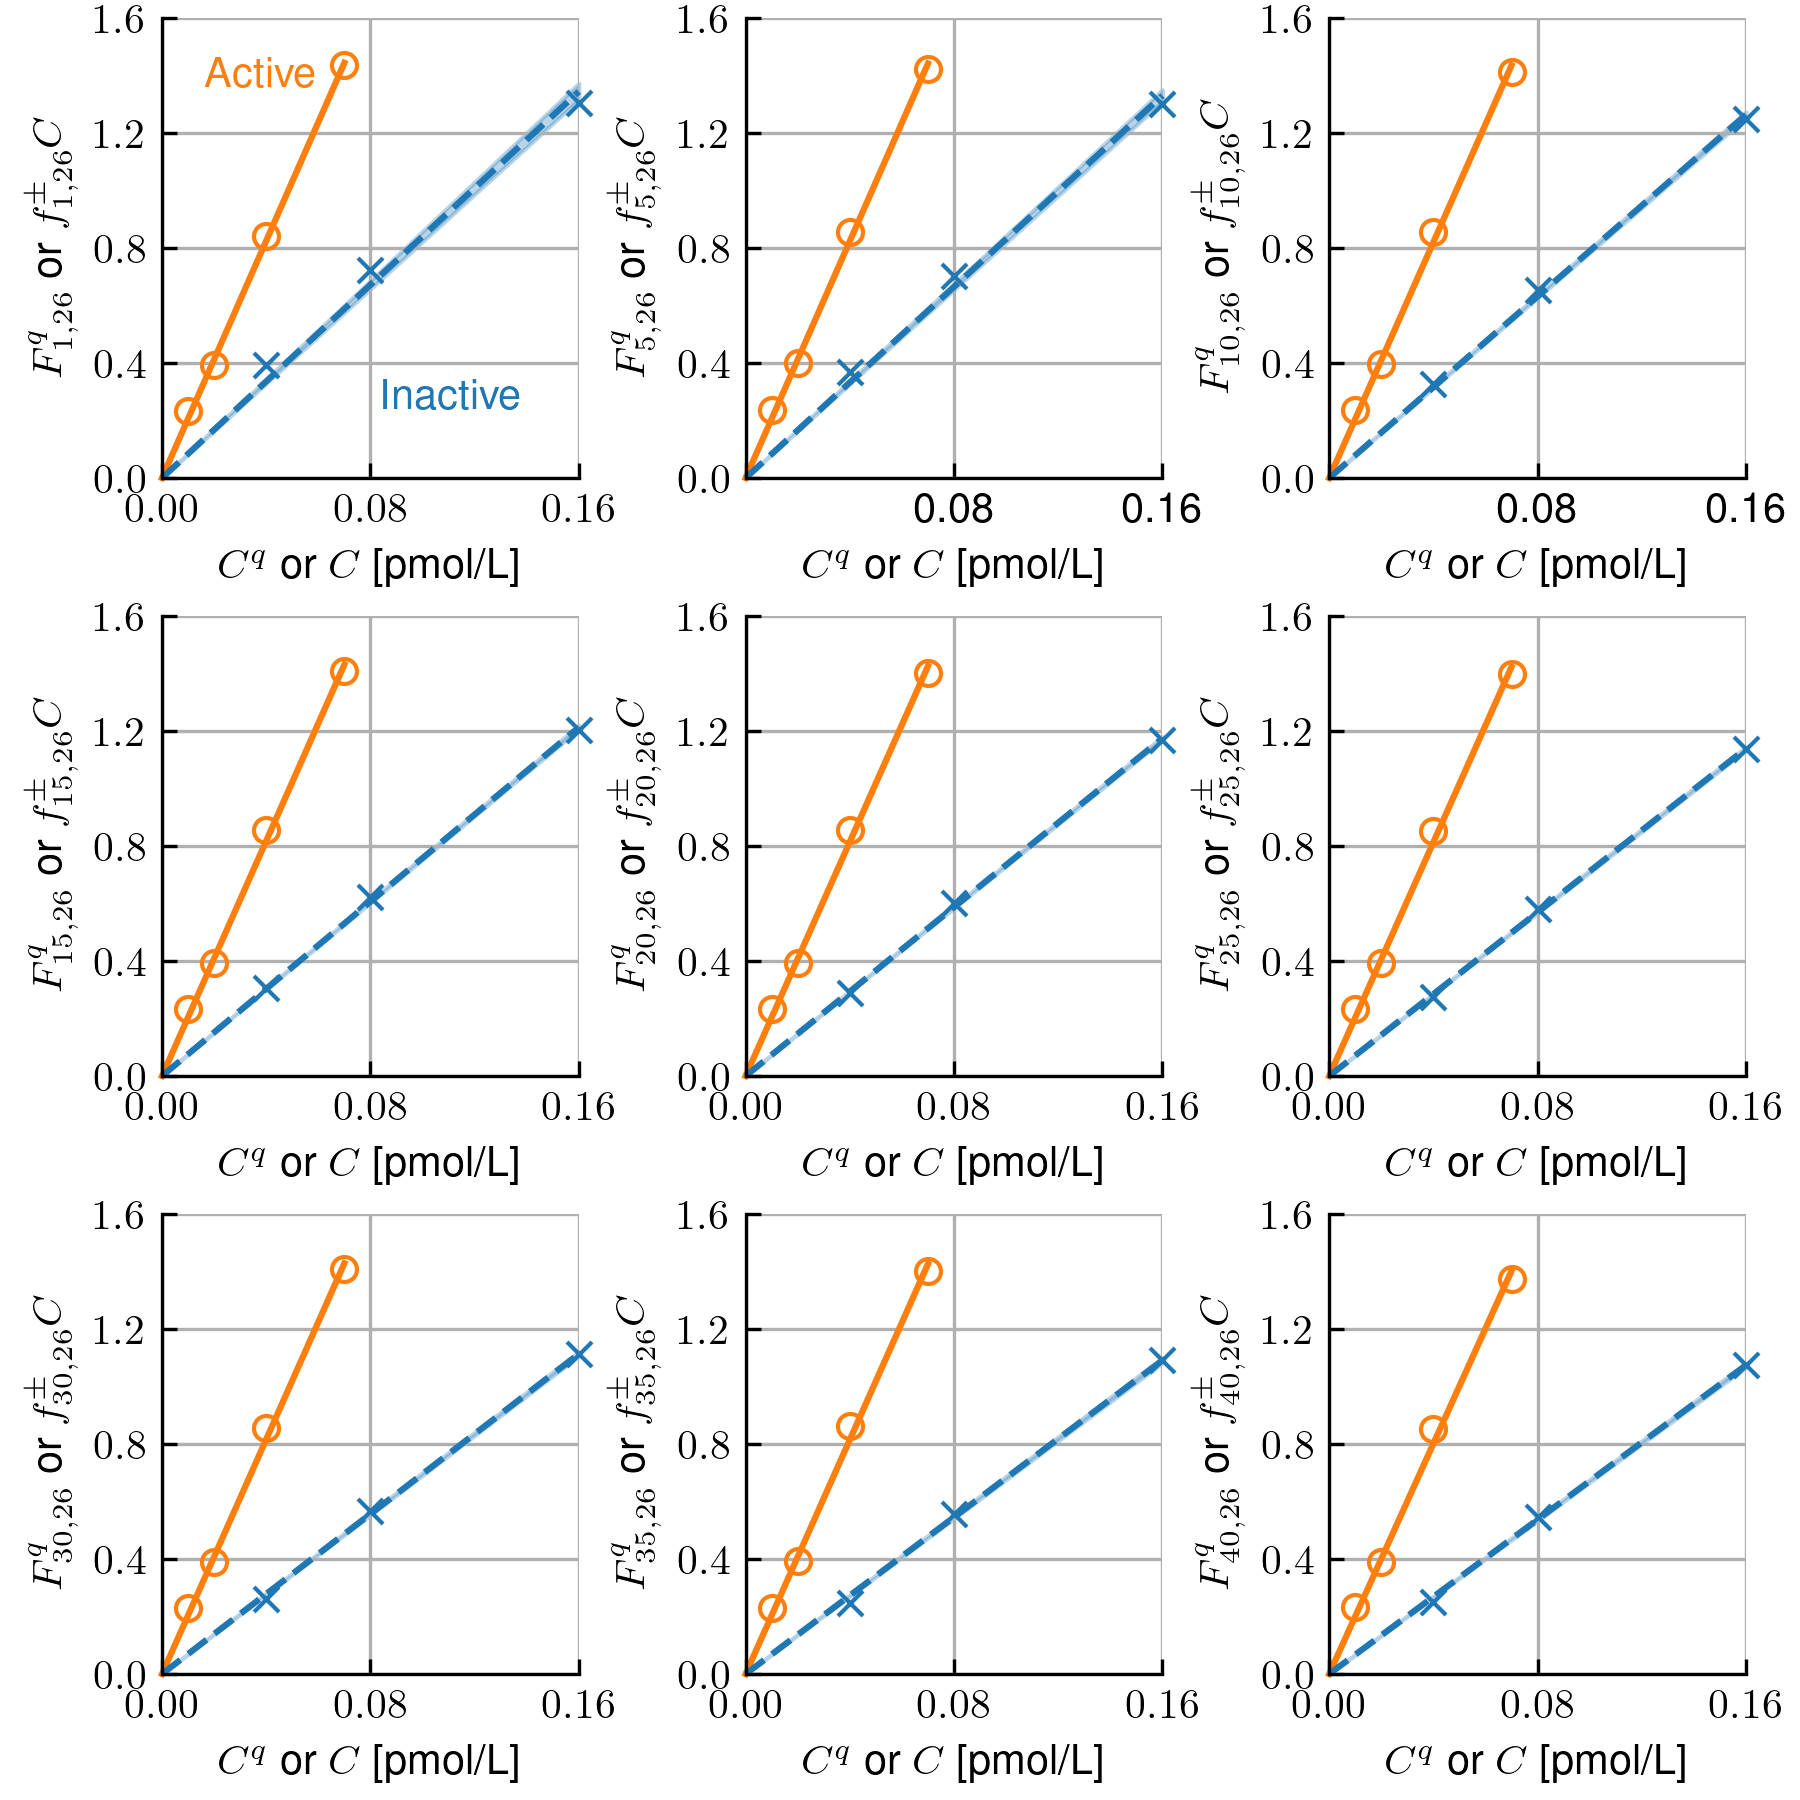
\includegraphics{si-figs/FigS26.png}
                    \caption{
                        As Figure~\ref{fig:S1} with well $w=26$ (or C2).
                    }
                \end{figure}
                \clearpage
    \begin{table}
        \caption{Molar Fluorescence Parameters for Well C2 ($w=26$)}
        \centering
        \begin{tabular}{c|ll|ll}
            Cycle & \multicolumn{2}{c|}{Inactive} & \multicolumn{2}{c}{Active} \\
            \hline
            $i$ & $f_{i,26}^{-}$ & $\sigma_{i,26}^{-}$ &  $f_{i,26}^{+}$ & $\sigma_{i,26}^{+}$ \\
            \hline
    1 & 8.40 & 0.060 & 20.63 & 0.022 \\
2 & 8.51 & 0.059 & 20.43 & 0.024 \\
3 & 8.56 & 0.055 & 20.52 & 0.028 \\
4 & 8.45 & 0.049 & 20.56 & 0.029 \\
5 & 8.31 & 0.043 & 20.60 & 0.028 \\
6 & 8.20 & 0.036 & 20.59 & 0.029 \\
7 & 8.12 & 0.030 & 20.56 & 0.030 \\
8 & 8.03 & 0.026 & 20.54 & 0.030 \\
9 & 7.95 & 0.024 & 20.54 & 0.031 \\
10 & 7.90 & 0.021 & 20.51 & 0.031 \\
11 & 7.82 & 0.019 & 20.48 & 0.031 \\
12 & 7.77 & 0.017 & 20.49 & 0.030 \\
13 & 7.69 & 0.016 & 20.46 & 0.032 \\
14 & 7.66 & 0.014 & 20.52 & 0.030 \\
15 & 7.58 & 0.014 & 20.45 & 0.032 \\
16 & 7.51 & 0.015 & 20.44 & 0.032 \\
17 & 7.45 & 0.014 & 20.40 & 0.033 \\
18 & 7.42 & 0.013 & 20.45 & 0.032 \\
19 & 7.39 & 0.011 & 20.39 & 0.032 \\
20 & 7.34 & 0.012 & 20.37 & 0.033 \\
21 & 7.29 & 0.013 & 20.44 & 0.031 \\
22 & 7.20 & 0.013 & 20.35 & 0.033 \\
23 & 7.22 & 0.011 & 20.33 & 0.033 \\
24 & 7.16 & 0.011 & 20.32 & 0.033 \\
25 & 7.12 & 0.011 & 20.33 & 0.033 \\
26 & 7.05 & 0.013 & 20.44 & 0.030 \\
27 & 7.02 & 0.014 & 20.36 & 0.032 \\
28 & 7.00 & 0.015 & 20.34 & 0.033 \\
29 & 6.97 & 0.014 & 20.29 & 0.033 \\
30 & 6.96 & 0.016 & 20.41 & 0.031 \\
31 & 6.97 & 0.023 & 20.36 & 0.035 \\
32 & 6.92 & 0.019 & 20.30 & 0.035 \\
33 & 6.90 & 0.017 & 20.21 & 0.036 \\
34 & 6.92 & 0.019 & 20.25 & 0.043 \\
35 & 6.82 & 0.019 & 20.38 & 0.035 \\
36 & 6.78 & 0.018 & 20.23 & 0.037 \\
37 & 6.83 & 0.019 & 20.04 & 0.040 \\
38 & 6.72 & 0.017 & 20.09 & 0.038 \\
39 & 6.77 & 0.015 & 20.05 & 0.039 \\
40 & 6.71 & 0.015 & 20.04 & 0.039 \\
41 & 6.63 & 0.021 & 20.03 & 0.039 \\
42 & 6.60 & 0.018 & 19.96 & 0.044 \\
43 & 6.60 & 0.017 & 19.92 & 0.043 \\
44 & 6.50 & 0.021 & 19.95 & 0.042 \\
45 & 6.55 & 0.019 & 19.92 & 0.042 \\
               \hline
        \end{tabular}
    \end{table}
    \clearpage

                \begin{figure}
                    \centering
                    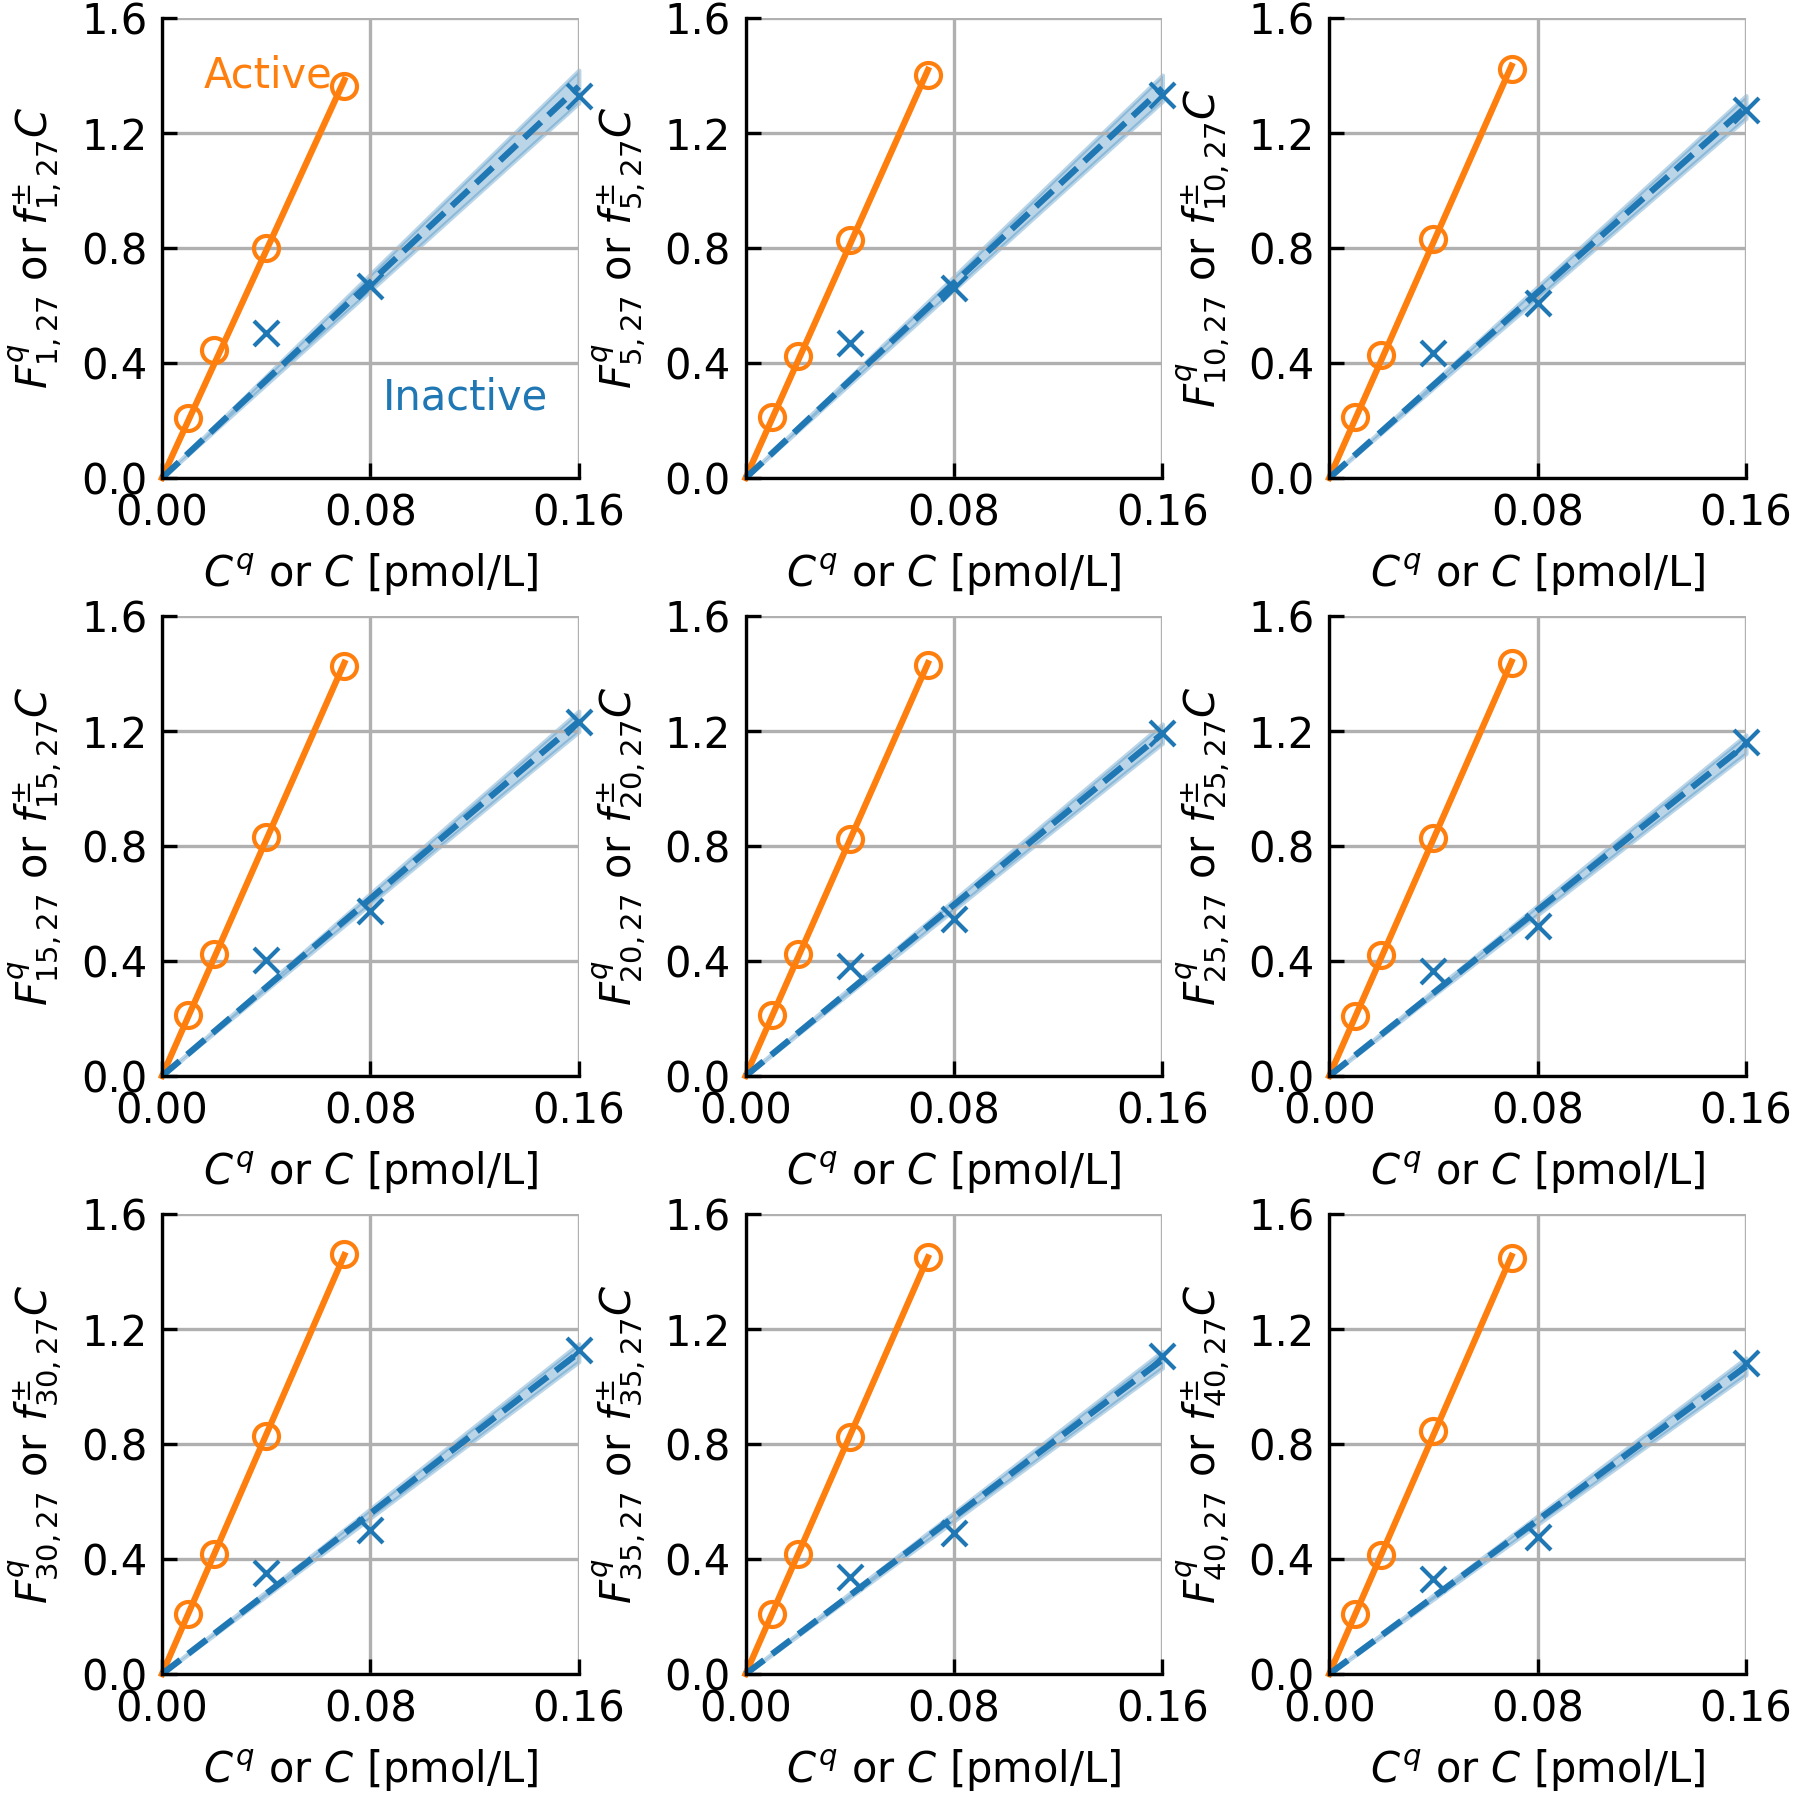
\includegraphics{si-figs/FigS27.png}
                    \caption{
                        As Figure~\ref{fig:S1} with well $w=27$ (or C3).
                    }
                \end{figure}
                \clearpage
    \begin{table}
        \caption{Molar Fluorescence Parameters for Well C3 ($w=27$)}
        \centering
        \begin{tabular}{c|ll|ll}
            Cycle & \multicolumn{2}{c|}{Inactive} & \multicolumn{2}{c}{Active} \\
            \hline
            $i$ & $f_{i,27}^{-}$ & $\sigma_{i,27}^{-}$ &  $f_{i,27}^{+}$ & $\sigma_{i,27}^{+}$ \\
            \hline
    1 & 8.5 & 0.12 & 19.78 & 0.032 \\
2 & 8.4 & 0.10 & 19.87 & 0.018 \\
3 & 8.6 & 0.10 & 20.09 & 0.018 \\
4 & 8.56 & 0.099 & 20.22 & 0.019 \\
5 & 8.47 & 0.095 & 20.28 & 0.019 \\
6 & 8.41 & 0.092 & 20.36 & 0.019 \\
7 & 8.33 & 0.089 & 20.41 & 0.018 \\
8 & 8.24 & 0.086 & 20.45 & 0.016 \\
9 & 8.15 & 0.083 & 20.50 & 0.016 \\
10 & 8.07 & 0.082 & 20.49 & 0.015 \\
11 & 7.98 & 0.080 & 20.51 & 0.014 \\
12 & 7.91 & 0.078 & 20.53 & 0.014 \\
13 & 7.85 & 0.077 & 20.53 & 0.013 \\
14 & 7.78 & 0.075 & 20.52 & 0.013 \\
15 & 7.71 & 0.075 & 20.53 & 0.012 \\
16 & 7.67 & 0.073 & 20.54 & 0.012 \\
17 & 7.60 & 0.072 & 20.55 & 0.011 \\
18 & 7.54 & 0.072 & 20.54 & 0.011 \\
19 & 7.49 & 0.071 & 20.54 & 0.010 \\
20 & 7.44 & 0.070 & 20.515 & 0.0096 \\
21 & 7.39 & 0.068 & 20.540 & 0.0096 \\
22 & 7.35 & 0.069 & 20.549 & 0.0089 \\
23 & 7.30 & 0.068 & 20.56 & 0.012 \\
24 & 7.26 & 0.068 & 20.526 & 0.0097 \\
25 & 7.21 & 0.067 & 20.597 & 0.0067 \\
26 & 7.18 & 0.068 & 20.569 & 0.0065 \\
27 & 7.12 & 0.066 & 20.539 & 0.0071 \\
28 & 7.06 & 0.064 & 20.602 & 0.0046 \\
29 & 7.02 & 0.065 & 20.580 & 0.0067 \\
30 & 6.98 & 0.066 & 20.817 & 0.0032 \\
31 & 6.96 & 0.061 & 20.595 & 0.0047 \\
32 & 6.92 & 0.061 & 20.879 & 0.0063 \\
33 & 6.89 & 0.059 & 20.760 & 0.0043 \\
34 & 6.86 & 0.059 & 20.753 & 0.0031 \\
35 & 6.83 & 0.060 & 20.701 & 0.0032 \\
36 & 6.79 & 0.059 & 20.767 & 0.0048 \\
37 & 6.77 & 0.060 & 20.811 & 0.0073 \\
38 & 6.75 & 0.061 & 20.90 & 0.010 \\
39 & 6.72 & 0.062 & 20.832 & 0.0082 \\
40 & 6.69 & 0.061 & 20.776 & 0.0091 \\
41 & 6.72 & 0.059 & 20.769 & 0.0096 \\
42 & 6.68 & 0.060 & 20.737 & 0.0092 \\
43 & 6.66 & 0.058 & 20.727 & 0.0071 \\
44 & 6.62 & 0.055 & 20.638 & 0.0087 \\
45 & 6.60 & 0.058 & 20.609 & 0.0092 \\
               \hline
        \end{tabular}
    \end{table}
    \clearpage

                \begin{figure}
                    \centering
                    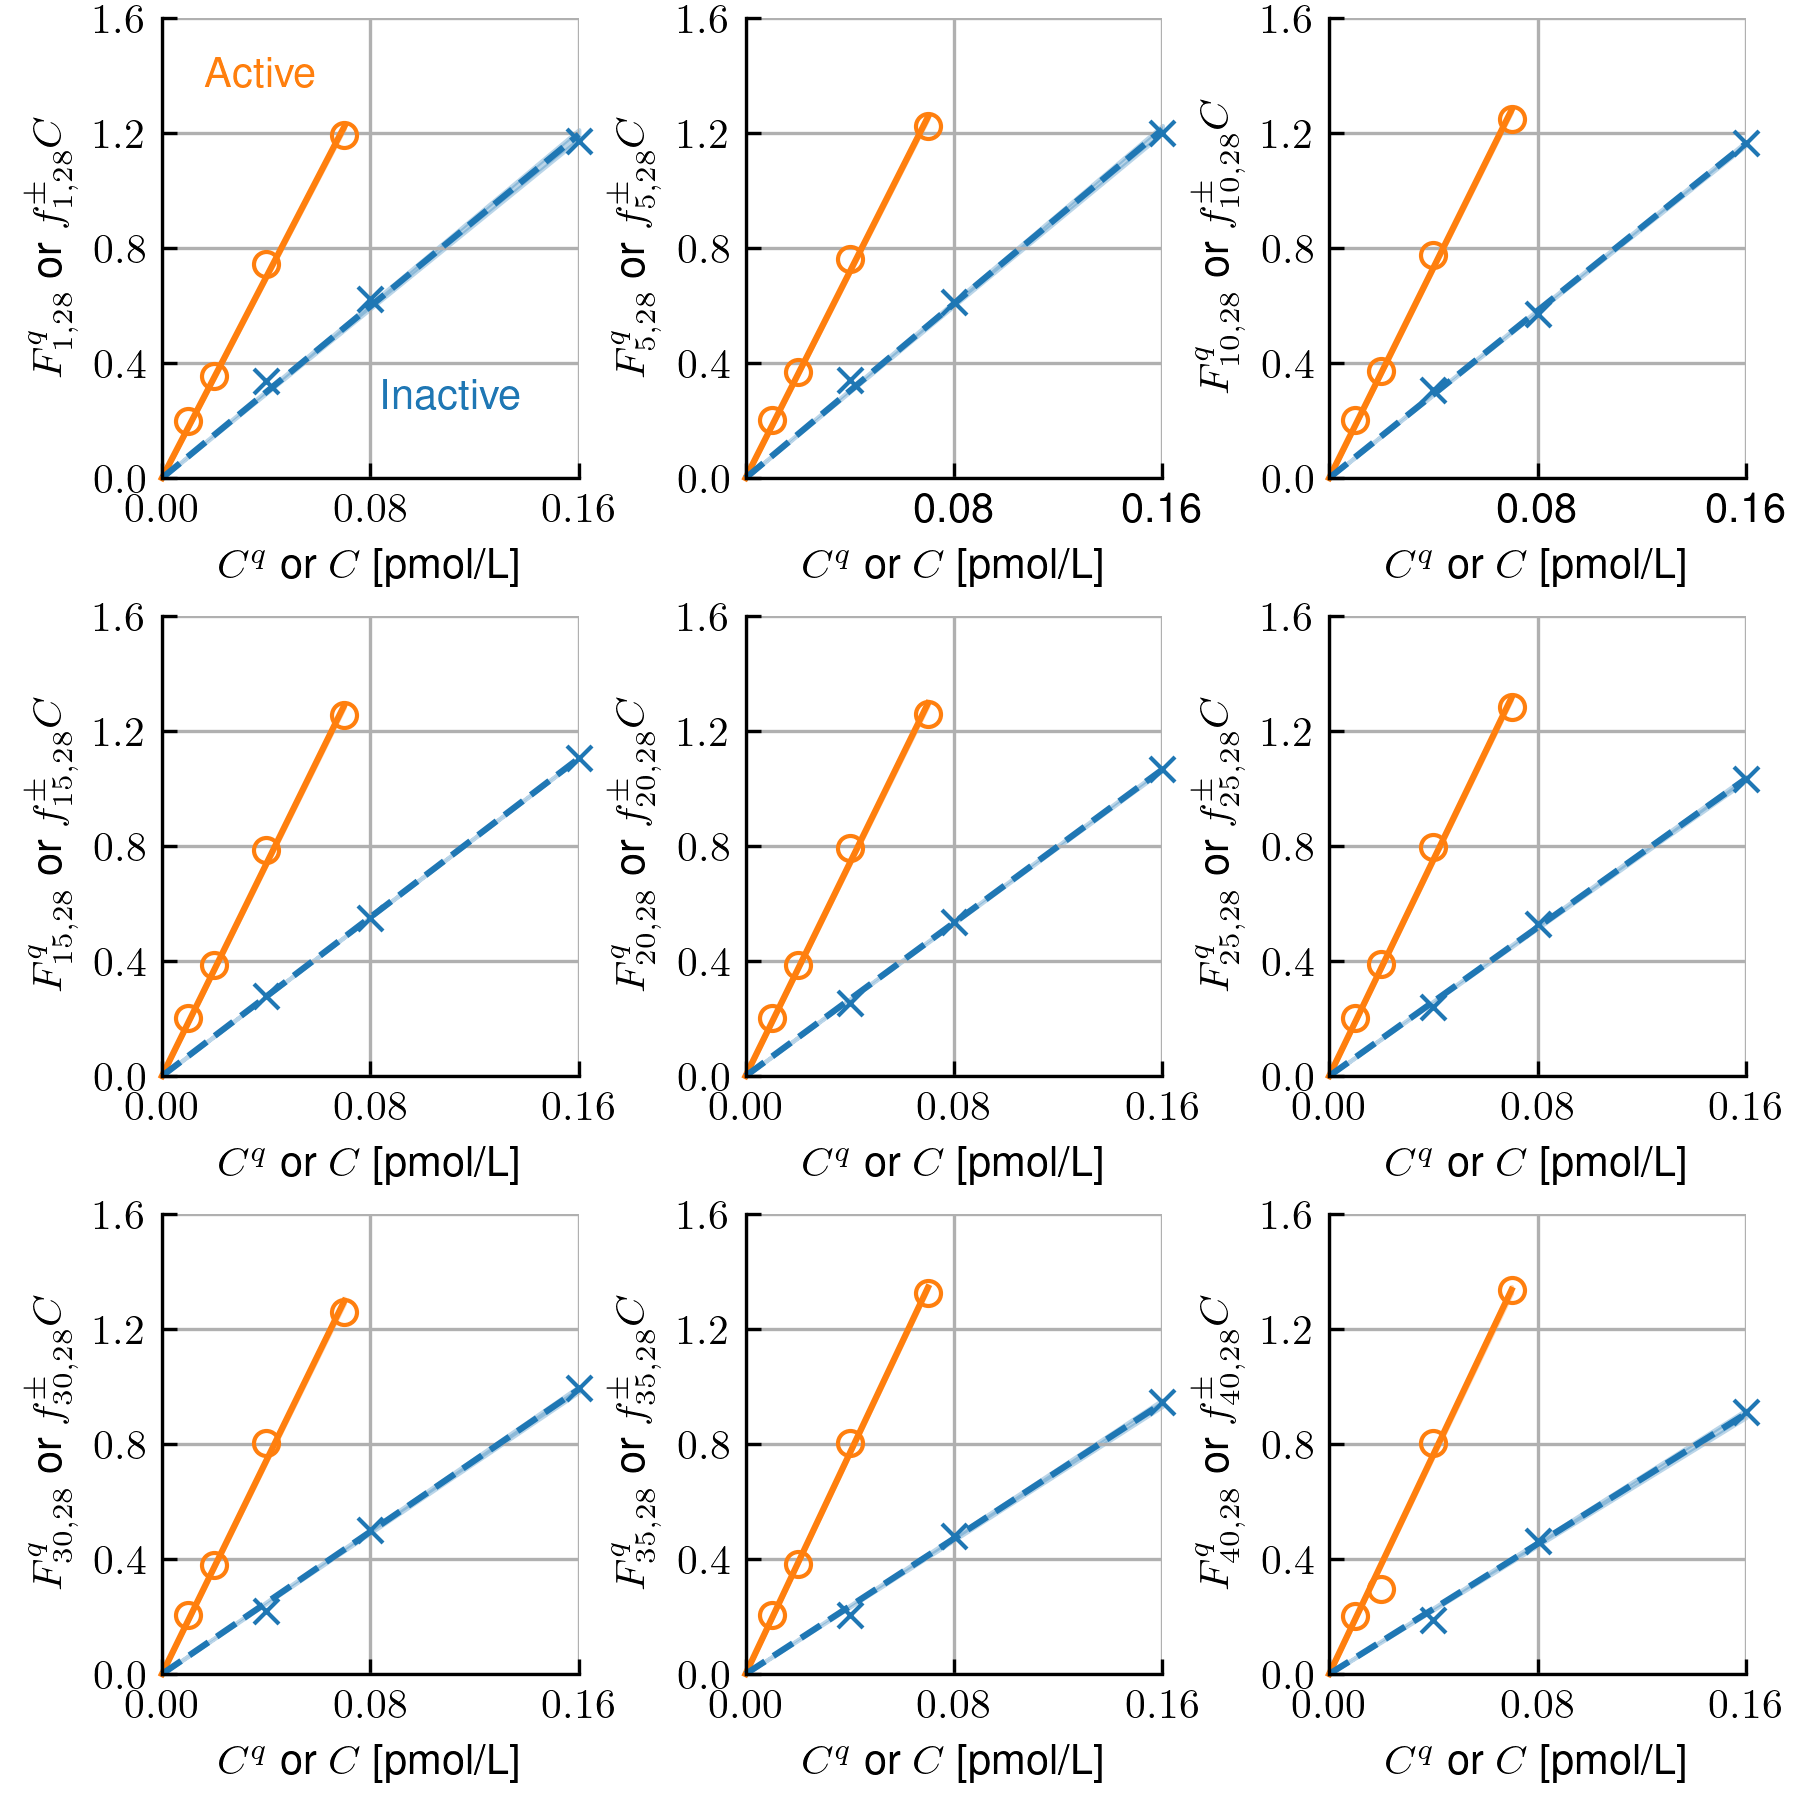
\includegraphics{si-figs/FigS28.png}
                    \caption{
                        As Figure~\ref{fig:S1} with well $w=28$ (or C4).
                    }
                \end{figure}
                \clearpage
    \begin{table}
        \caption{Molar Fluorescence Parameters for Well C4 ($w=28$)}
        \centering
        \begin{tabular}{c|ll|ll}
            Cycle & \multicolumn{2}{c|}{Inactive} & \multicolumn{2}{c}{Active} \\
            \hline
            $i$ & $f_{i,28}^{-}$ & $\sigma_{i,28}^{-}$ &  $f_{i,28}^{+}$ & $\sigma_{i,28}^{+}$ \\
            \hline
    1 & 7.47 & 0.035 & 17.47 & 0.034 \\
2 & 7.40 & 0.038 & 17.34 & 0.036 \\
3 & 7.55 & 0.036 & 17.57 & 0.037 \\
4 & 7.59 & 0.033 & 17.78 & 0.034 \\
5 & 7.58 & 0.029 & 17.94 & 0.034 \\
6 & 7.54 & 0.024 & 18.04 & 0.034 \\
7 & 7.47 & 0.021 & 18.13 & 0.033 \\
8 & 7.40 & 0.018 & 18.21 & 0.032 \\
9 & 7.33 & 0.014 & 18.24 & 0.033 \\
10 & 7.27 & 0.013 & 18.28 & 0.033 \\
11 & 7.18 & 0.010 & 18.36 & 0.031 \\
12 & 7.107 & 0.0074 & 18.31 & 0.034 \\
13 & 7.052 & 0.0047 & 18.39 & 0.035 \\
14 & 6.988 & 0.0040 & 18.41 & 0.036 \\
15 & 6.906 & 0.0017 & 18.43 & 0.038 \\
16 & 6.856 & 0.0013 & 18.44 & 0.039 \\
17 & 6.816 & 0.0024 & 18.48 & 0.039 \\
18 & 6.763 & 0.0044 & 18.54 & 0.039 \\
19 & 6.726 & 0.0066 & 18.51 & 0.041 \\
20 & 6.663 & 0.0082 & 18.52 & 0.040 \\
21 & 6.630 & 0.0098 & 18.55 & 0.040 \\
22 & 6.57 & 0.011 & 18.62 & 0.040 \\
23 & 6.53 & 0.012 & 18.61 & 0.040 \\
24 & 6.50 & 0.015 & 18.67 & 0.039 \\
25 & 6.46 & 0.016 & 18.80 & 0.034 \\
26 & 6.43 & 0.017 & 18.79 & 0.035 \\
27 & 6.28 & 0.014 & 18.69 & 0.039 \\
28 & 6.25 & 0.018 & 18.77 & 0.037 \\
29 & 6.23 & 0.019 & 18.75 & 0.037 \\
30 & 6.19 & 0.020 & 18.54 & 0.044 \\
31 & 6.15 & 0.022 & 18.54 & 0.045 \\
32 & 6.13 & 0.024 & 18.55 & 0.043 \\
33 & 6.09 & 0.026 & 19.17 & 0.025 \\
34 & 6.07 & 0.027 & 19.15 & 0.025 \\
35 & 5.89 & 0.024 & 19.21 & 0.024 \\
36 & 5.86 & 0.024 & 19.26 & 0.023 \\
37 & 5.80 & 0.026 & 18.97 & 0.057 \\
38 & 5.76 & 0.026 & 19.04 & 0.055 \\
39 & 5.70 & 0.026 & 19.08 & 0.055 \\
40 & 5.66 & 0.027 & 19.09 & 0.056 \\
41 & 5.63 & 0.030 & 19.14 & 0.056 \\
42 & 5.60 & 0.031 & 19.20 & 0.056 \\
43 & 5.57 & 0.031 & 19.35 & 0.062 \\
44 & 5.54 & 0.032 & 19.37 & 0.066 \\
45 & 5.51 & 0.032 & 19.15 & 0.067 \\
               \hline
        \end{tabular}
    \end{table}
    \clearpage

                \begin{figure}
                    \centering
                    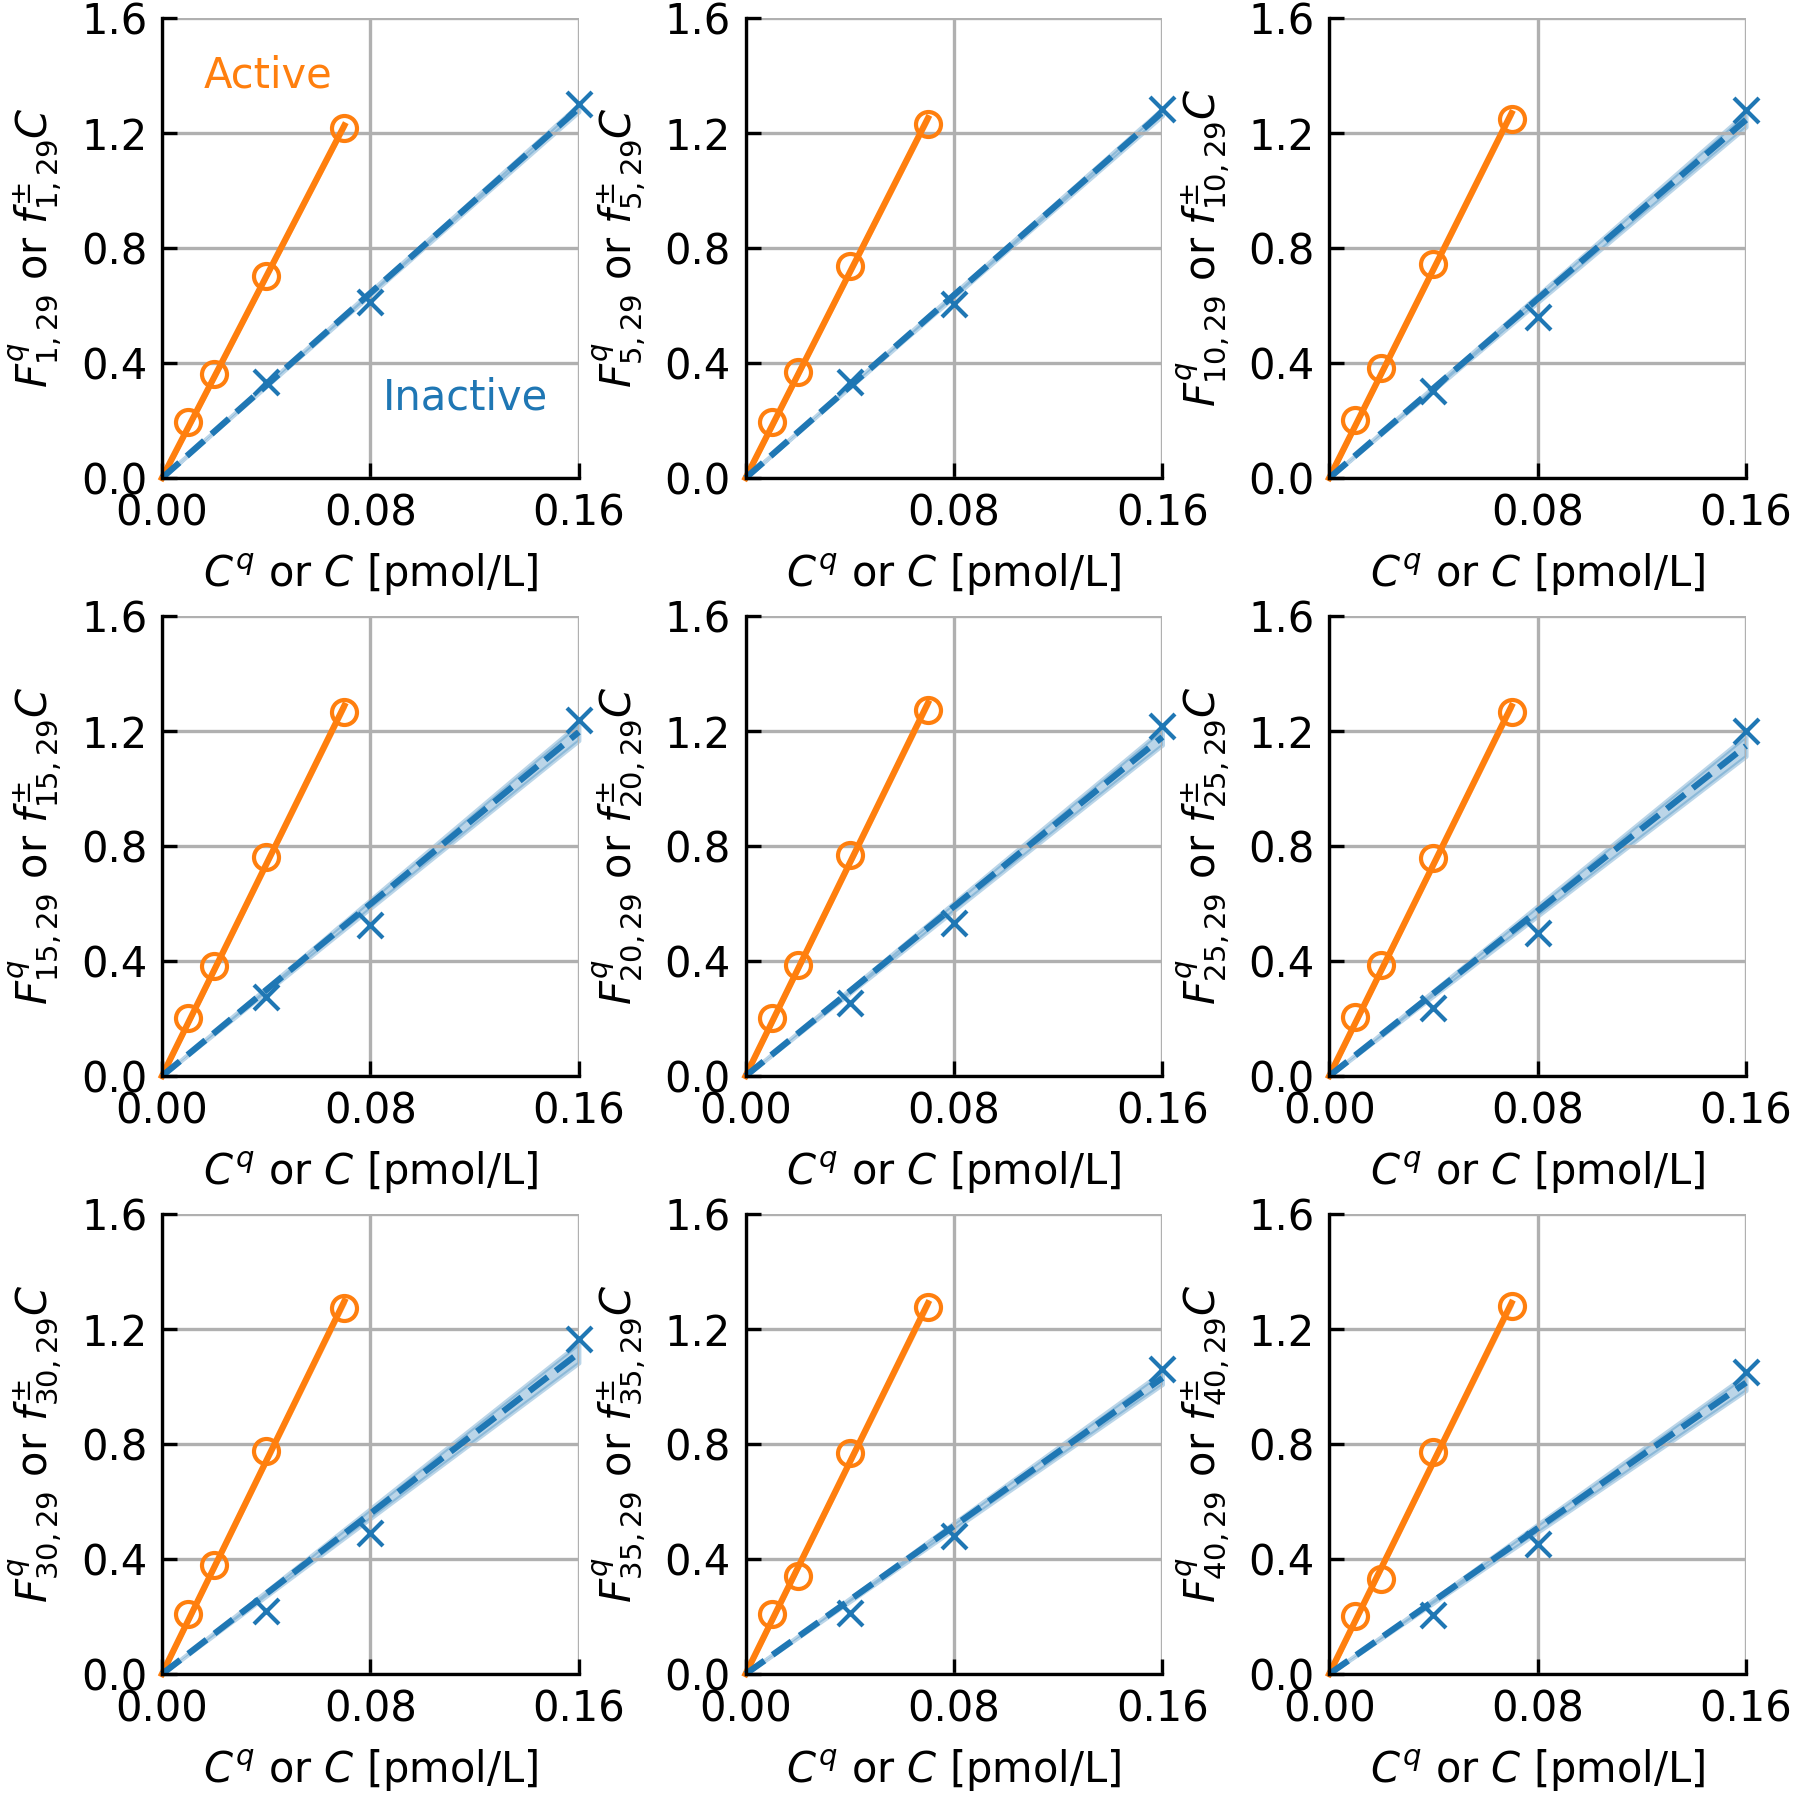
\includegraphics{si-figs/FigS29.png}
                    \caption{
                        As Figure~\ref{fig:S1} with well $w=29$ (or C5).
                    }
                \end{figure}
                \clearpage
    \begin{table}
        \caption{Molar Fluorescence Parameters for Well C5 ($w=29$)}
        \centering
        \begin{tabular}{c|ll|ll}
            Cycle & \multicolumn{2}{c|}{Inactive} & \multicolumn{2}{c}{Active} \\
            \hline
            $i$ & $f_{i,29}^{-}$ & $\sigma_{i,29}^{-}$ &  $f_{i,29}^{+}$ & $\sigma_{i,29}^{+}$ \\
            \hline
    1 & 8.04 & 0.026 & 17.52 & 0.013 \\
2 & 7.82 & 0.021 & 17.44 & 0.020 \\
3 & 7.95 & 0.019 & 17.61 & 0.021 \\
4 & 7.99 & 0.023 & 17.77 & 0.020 \\
5 & 7.95 & 0.026 & 17.88 & 0.021 \\
6 & 7.89 & 0.029 & 18.00 & 0.020 \\
7 & 7.91 & 0.038 & 18.07 & 0.021 \\
8 & 7.89 & 0.045 & 18.07 & 0.023 \\
9 & 7.85 & 0.049 & 18.10 & 0.023 \\
10 & 7.79 & 0.052 & 18.13 & 0.022 \\
11 & 7.71 & 0.053 & 18.27 & 0.019 \\
12 & 7.65 & 0.055 & 18.27 & 0.019 \\
13 & 7.60 & 0.057 & 18.29 & 0.020 \\
14 & 7.53 & 0.060 & 18.35 & 0.022 \\
15 & 7.48 & 0.062 & 18.40 & 0.024 \\
16 & 7.47 & 0.053 & 18.43 & 0.025 \\
17 & 7.44 & 0.051 & 18.41 & 0.027 \\
18 & 7.43 & 0.055 & 18.52 & 0.024 \\
19 & 7.40 & 0.056 & 18.52 & 0.025 \\
20 & 7.37 & 0.057 & 18.53 & 0.025 \\
21 & 7.31 & 0.056 & 18.59 & 0.026 \\
22 & 7.27 & 0.058 & 18.58 & 0.026 \\
23 & 7.23 & 0.065 & 18.45 & 0.030 \\
24 & 7.18 & 0.073 & 18.36 & 0.024 \\
25 & 7.17 & 0.074 & 18.38 & 0.024 \\
26 & 7.11 & 0.071 & 18.42 & 0.023 \\
27 & 7.06 & 0.070 & 18.44 & 0.024 \\
28 & 7.04 & 0.070 & 18.46 & 0.025 \\
29 & 7.01 & 0.070 & 18.47 & 0.026 \\
30 & 6.98 & 0.071 & 18.52 & 0.029 \\
31 & 6.54 & 0.042 & 18.49 & 0.025 \\
32 & 6.50 & 0.046 & 18.39 & 0.030 \\
33 & 6.49 & 0.046 & 18.41 & 0.028 \\
34 & 6.47 & 0.046 & 18.42 & 0.028 \\
35 & 6.44 & 0.046 & 18.42 & 0.029 \\
36 & 6.42 & 0.048 & 18.36 & 0.031 \\
37 & 6.42 & 0.049 & 18.38 & 0.029 \\
38 & 6.37 & 0.060 & 18.41 & 0.030 \\
39 & 6.37 & 0.058 & 18.43 & 0.031 \\
40 & 6.33 & 0.057 & 18.44 & 0.032 \\
41 & 6.33 & 0.057 & 17.88 & 0.042 \\
42 & 6.32 & 0.058 & 17.79 & 0.052 \\
43 & 6.30 & 0.059 & 17.79 & 0.052 \\
44 & 6.28 & 0.058 & 17.58 & 0.052 \\
45 & 6.23 & 0.060 & 17.56 & 0.053 \\
               \hline
        \end{tabular}
    \end{table}
    \clearpage

                \begin{figure}
                    \centering
                    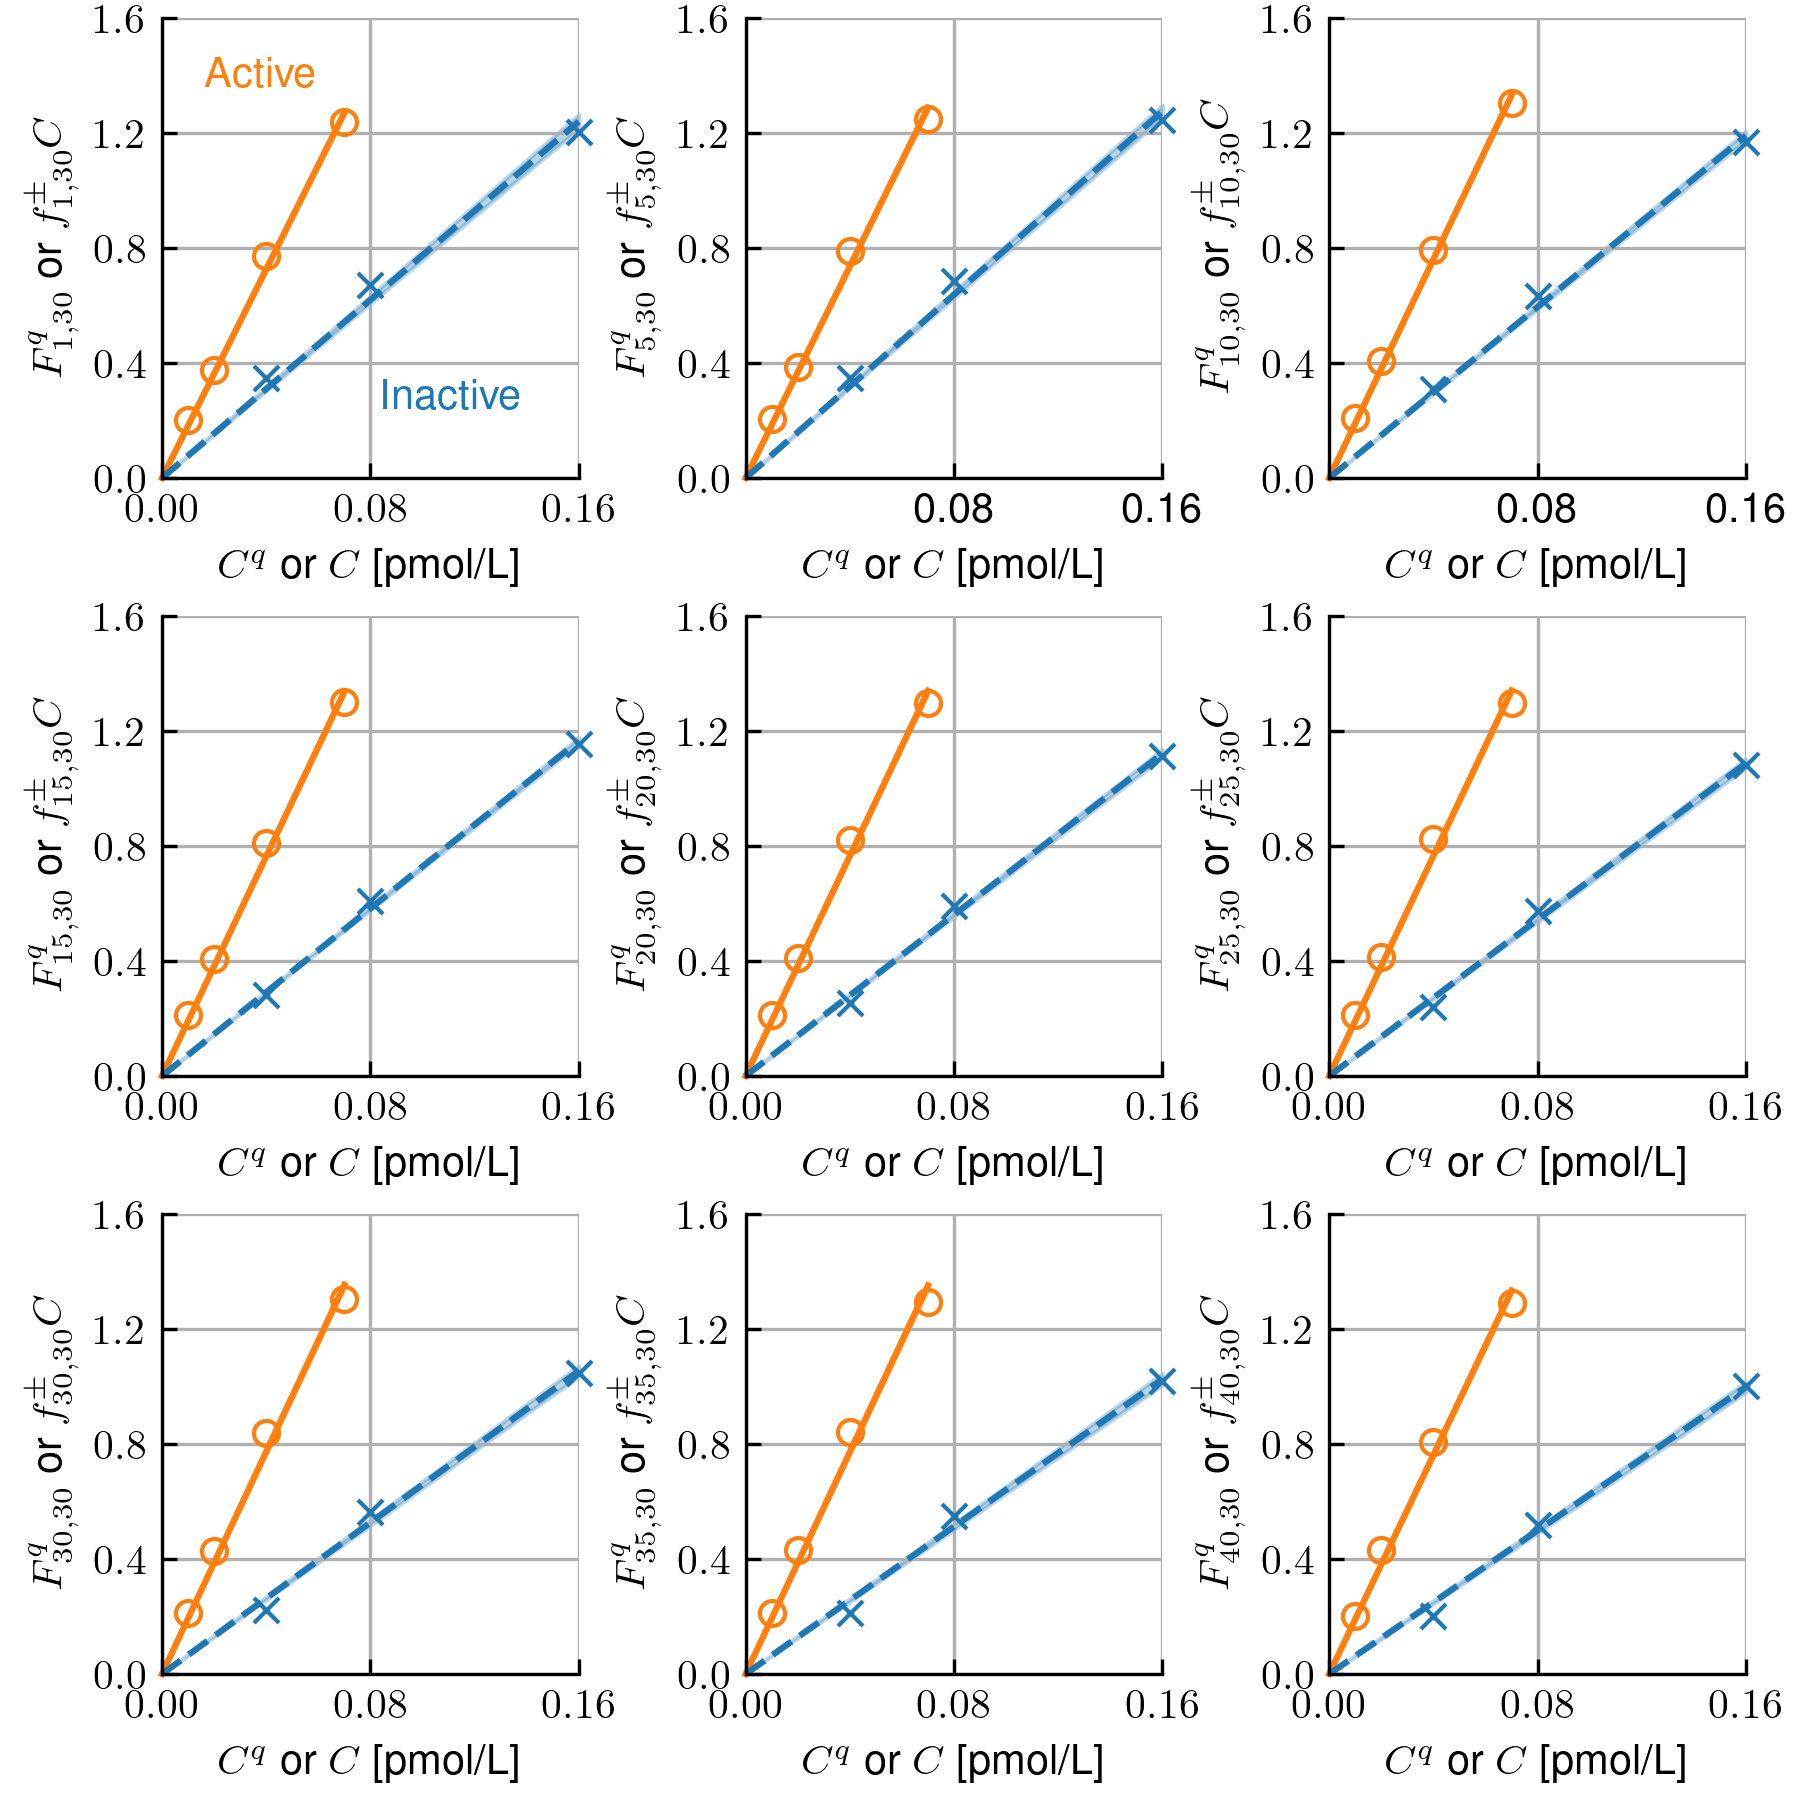
\includegraphics{si-figs/FigS30.png}
                    \caption{
                        As Figure~\ref{fig:S1} with well $w=30$ (or C6).
                    }
                \end{figure}
                \clearpage
    \begin{table}
        \caption{Molar Fluorescence Parameters for Well C6 ($w=30$)}
        \centering
        \begin{tabular}{c|ll|ll}
            Cycle & \multicolumn{2}{c|}{Inactive} & \multicolumn{2}{c}{Active} \\
            \hline
            $i$ & $f_{i,30}^{-}$ & $\sigma_{i,30}^{-}$ &  $f_{i,30}^{+}$ & $\sigma_{i,30}^{+}$ \\
            \hline
    1 & 7.75 & 0.051 & 18.15 & 0.036 \\
2 & 7.78 & 0.044 & 17.89 & 0.039 \\
3 & 7.89 & 0.047 & 18.09 & 0.041 \\
4 & 7.97 & 0.048 & 18.28 & 0.040 \\
5 & 7.97 & 0.045 & 18.39 & 0.042 \\
6 & 7.90 & 0.042 & 18.38 & 0.046 \\
7 & 7.79 & 0.037 & 18.69 & 0.038 \\
8 & 7.68 & 0.036 & 18.89 & 0.033 \\
9 & 7.57 & 0.033 & 18.96 & 0.031 \\
10 & 7.44 & 0.031 & 19.02 & 0.031 \\
11 & 7.45 & 0.027 & 19.06 & 0.030 \\
12 & 7.43 & 0.025 & 19.09 & 0.034 \\
13 & 7.39 & 0.022 & 19.12 & 0.035 \\
14 & 7.35 & 0.022 & 19.11 & 0.037 \\
15 & 7.29 & 0.022 & 19.10 & 0.038 \\
16 & 7.22 & 0.023 & 19.11 & 0.039 \\
17 & 7.18 & 0.025 & 19.14 & 0.039 \\
18 & 7.12 & 0.026 & 19.14 & 0.040 \\
19 & 7.07 & 0.027 & 19.12 & 0.042 \\
20 & 7.01 & 0.029 & 19.13 & 0.044 \\
21 & 6.95 & 0.031 & 19.15 & 0.045 \\
22 & 6.90 & 0.028 & 19.16 & 0.045 \\
23 & 6.92 & 0.029 & 19.12 & 0.046 \\
24 & 6.88 & 0.030 & 19.15 & 0.048 \\
25 & 6.80 & 0.031 & 19.15 & 0.047 \\
26 & 6.74 & 0.031 & 19.15 & 0.047 \\
27 & 6.71 & 0.034 & 19.14 & 0.047 \\
28 & 6.67 & 0.033 & 19.20 & 0.051 \\
29 & 6.62 & 0.037 & 19.22 & 0.055 \\
30 & 6.59 & 0.038 & 19.33 & 0.053 \\
31 & 6.54 & 0.039 & 19.36 & 0.052 \\
32 & 6.52 & 0.039 & 19.37 & 0.056 \\
33 & 6.50 & 0.041 & 19.33 & 0.057 \\
34 & 6.46 & 0.041 & 19.32 & 0.057 \\
35 & 6.41 & 0.041 & 19.30 & 0.059 \\
36 & 6.37 & 0.035 & 19.35 & 0.061 \\
37 & 6.36 & 0.036 & 19.25 & 0.057 \\
38 & 6.30 & 0.037 & 19.25 & 0.059 \\
39 & 6.27 & 0.037 & 19.24 & 0.059 \\
40 & 6.24 & 0.036 & 19.04 & 0.046 \\
41 & 6.23 & 0.037 & 18.94 & 0.039 \\
42 & 6.20 & 0.038 & 18.95 & 0.040 \\
43 & 6.18 & 0.039 & 18.54 & 0.053 \\
44 & 6.09 & 0.041 & 18.50 & 0.056 \\
45 & 5.85 & 0.033 & 18.48 & 0.055 \\
               \hline
        \end{tabular}
    \end{table}
    \clearpage

                \begin{figure}
                    \centering
                    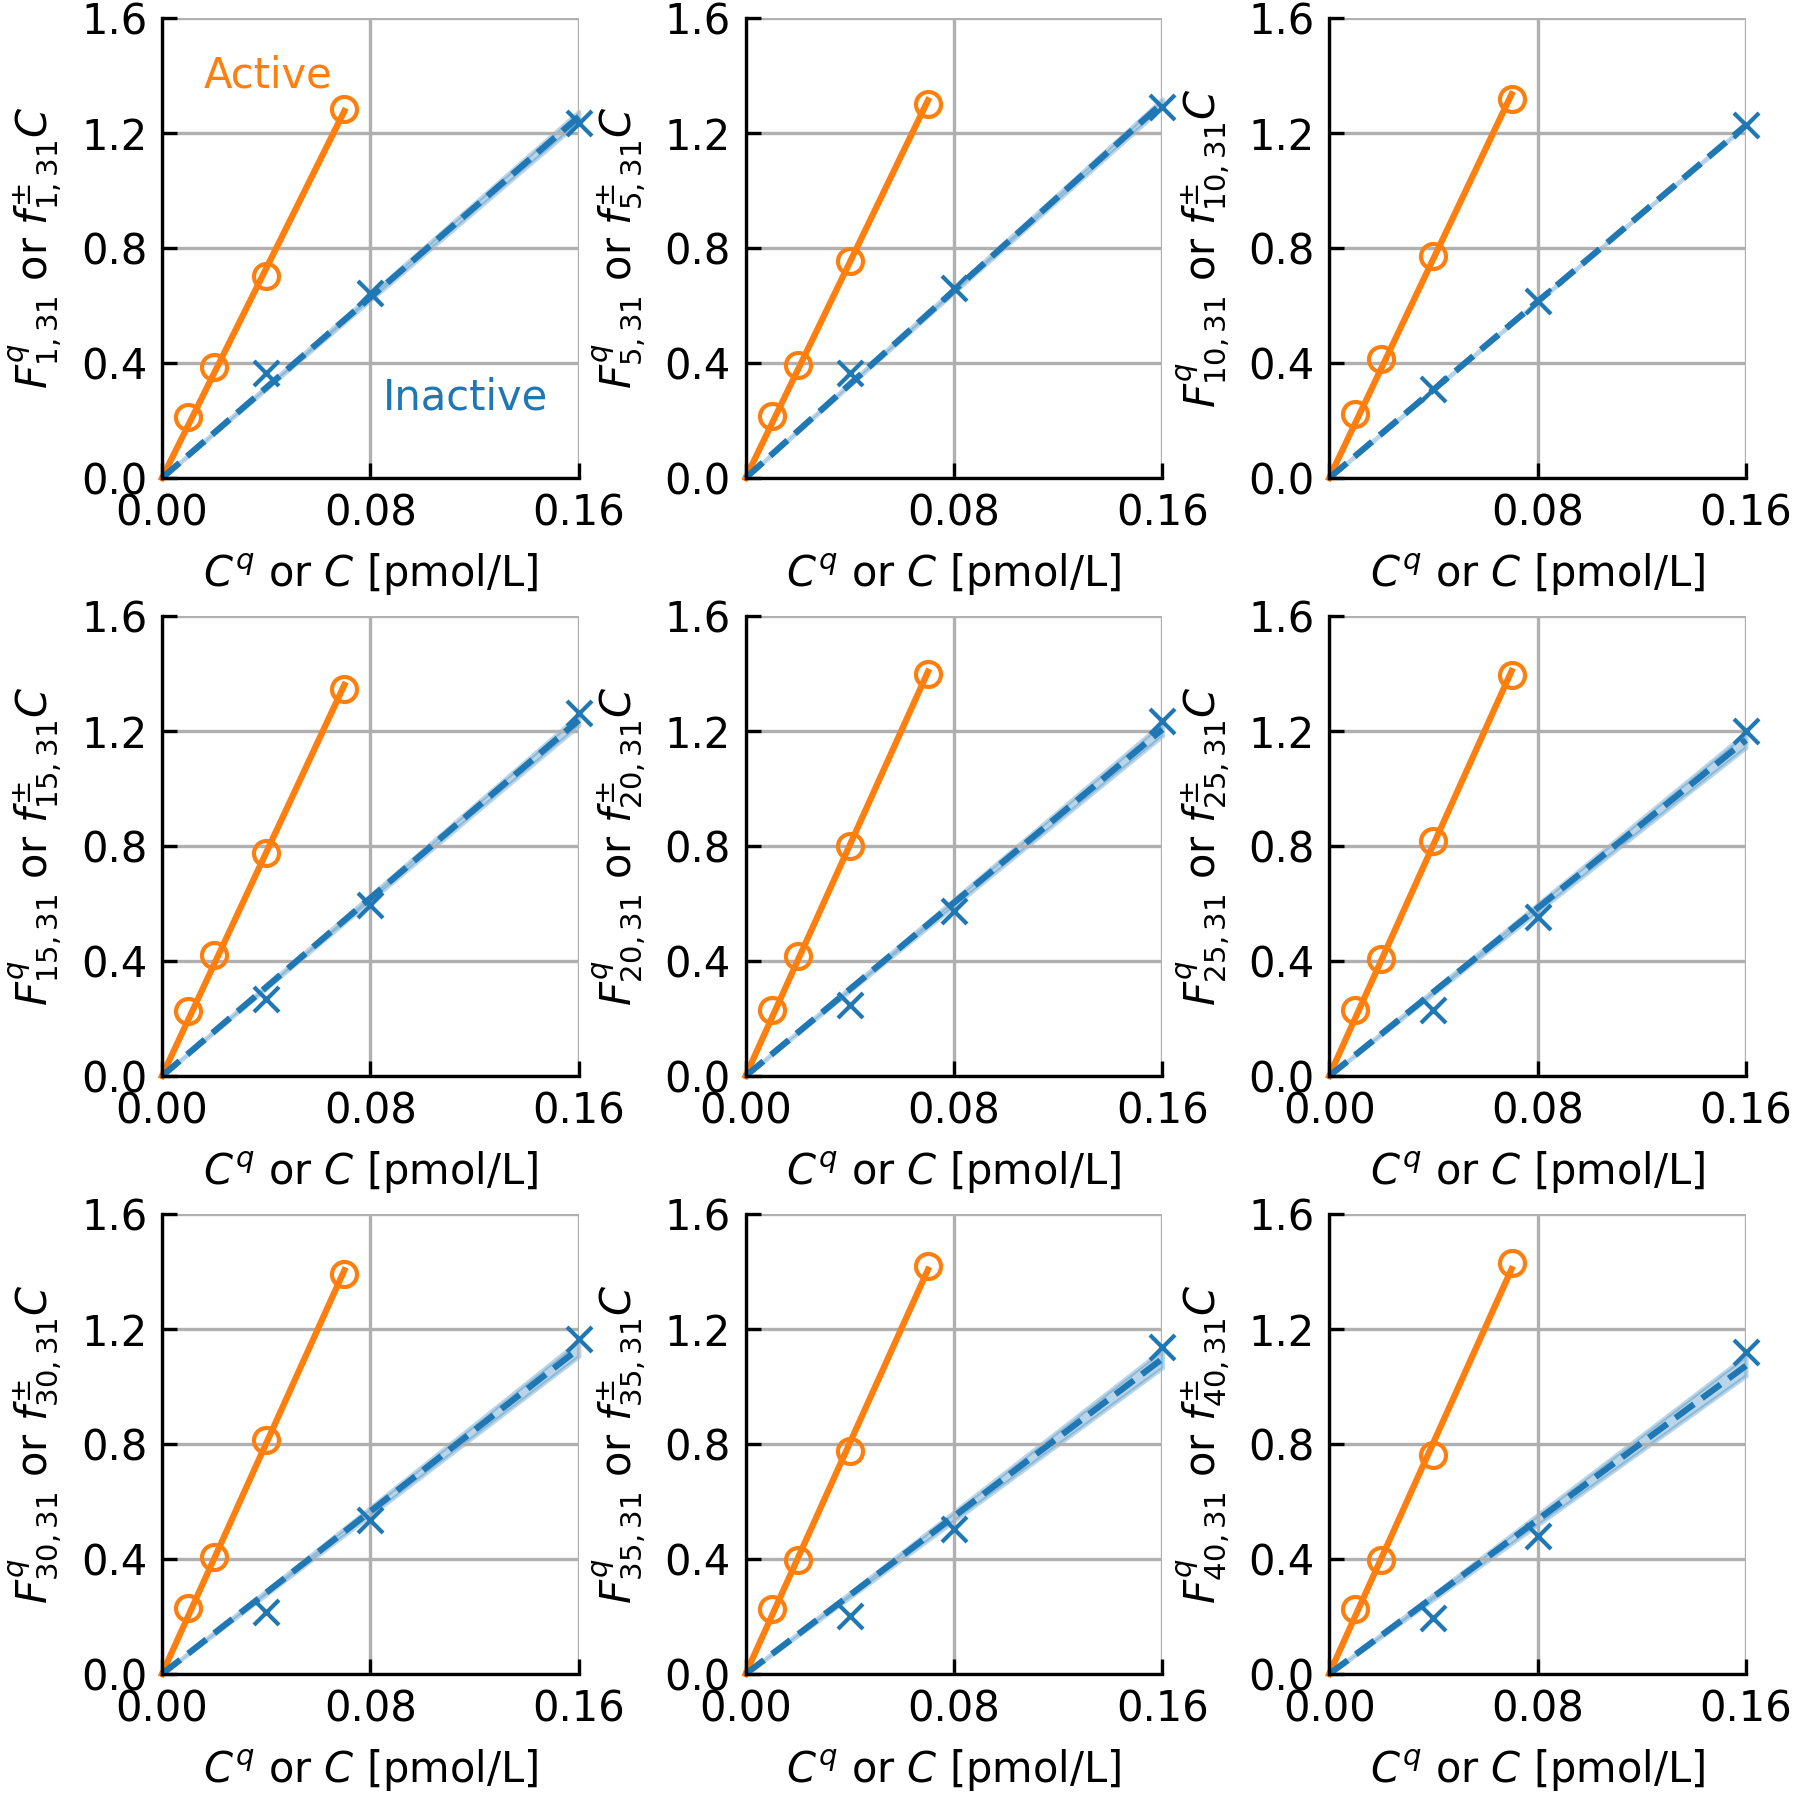
\includegraphics{si-figs/FigS31.png}
                    \caption{
                        As Figure~\ref{fig:S1} with well $w=31$ (or C7).
                    }
                \end{figure}
                \clearpage
    \begin{table}
        \caption{Molar Fluorescence Parameters for Well C7 ($w=31$)}
        \centering
        \begin{tabular}{c|ll|ll}
            Cycle & \multicolumn{2}{c|}{Inactive} & \multicolumn{2}{c}{Active} \\
            \hline
            $i$ & $f_{i,31}^{-}$ & $\sigma_{i,31}^{-}$ &  $f_{i,31}^{+}$ & $\sigma_{i,31}^{+}$ \\
            \hline
    1 & 7.85 & 0.039 & 18.24 & 0.026 \\
2 & 7.86 & 0.032 & 17.99 & 0.020 \\
3 & 8.02 & 0.035 & 18.27 & 0.020 \\
4 & 8.16 & 0.033 & 18.54 & 0.020 \\
5 & 8.15 & 0.029 & 18.77 & 0.020 \\
6 & 8.08 & 0.024 & 18.87 & 0.020 \\
7 & 7.96 & 0.019 & 18.92 & 0.021 \\
8 & 7.84 & 0.013 & 18.98 & 0.023 \\
9 & 7.754 & 0.0073 & 19.00 & 0.025 \\
10 & 7.669 & 0.0017 & 19.07 & 0.028 \\
11 & 7.81 & 0.016 & 19.10 & 0.030 \\
12 & 7.78 & 0.022 & 19.09 & 0.031 \\
13 & 7.78 & 0.029 & 19.10 & 0.032 \\
14 & 7.76 & 0.035 & 19.11 & 0.032 \\
15 & 7.74 & 0.039 & 19.43 & 0.027 \\
16 & 7.70 & 0.042 & 19.74 & 0.023 \\
17 & 7.68 & 0.042 & 19.82 & 0.023 \\
18 & 7.65 & 0.045 & 19.87 & 0.023 \\
19 & 7.61 & 0.046 & 19.92 & 0.022 \\
20 & 7.54 & 0.047 & 20.09 & 0.019 \\
21 & 7.53 & 0.051 & 20.10 & 0.019 \\
22 & 7.49 & 0.054 & 20.15 & 0.019 \\
23 & 7.41 & 0.053 & 20.09 & 0.020 \\
24 & 7.37 & 0.055 & 20.21 & 0.018 \\
25 & 7.30 & 0.054 & 20.12 & 0.019 \\
26 & 7.18 & 0.050 & 20.16 & 0.020 \\
27 & 7.11 & 0.052 & 20.18 & 0.019 \\
28 & 7.09 & 0.053 & 20.20 & 0.019 \\
29 & 7.09 & 0.057 & 20.18 & 0.018 \\
30 & 7.07 & 0.056 & 20.06 & 0.020 \\
31 & 7.01 & 0.060 & 20.17 & 0.016 \\
32 & 6.98 & 0.062 & 20.12 & 0.017 \\
33 & 6.97 & 0.065 & 20.09 & 0.020 \\
34 & 6.91 & 0.064 & 20.06 & 0.021 \\
35 & 6.85 & 0.066 & 20.09 & 0.023 \\
36 & 6.82 & 0.067 & 20.09 & 0.024 \\
37 & 6.79 & 0.070 & 20.10 & 0.027 \\
38 & 6.75 & 0.072 & 20.12 & 0.029 \\
39 & 6.72 & 0.073 & 20.14 & 0.031 \\
40 & 6.70 & 0.074 & 20.12 & 0.032 \\
41 & 6.63 & 0.070 & 19.89 & 0.028 \\
42 & 6.56 & 0.069 & 19.75 & 0.021 \\
43 & 6.49 & 0.068 & 19.83 & 0.027 \\
44 & 6.44 & 0.070 & 19.85 & 0.027 \\
45 & 6.41 & 0.070 & 19.86 & 0.029 \\
               \hline
        \end{tabular}
    \end{table}
    \clearpage

                \begin{figure}
                    \centering
                    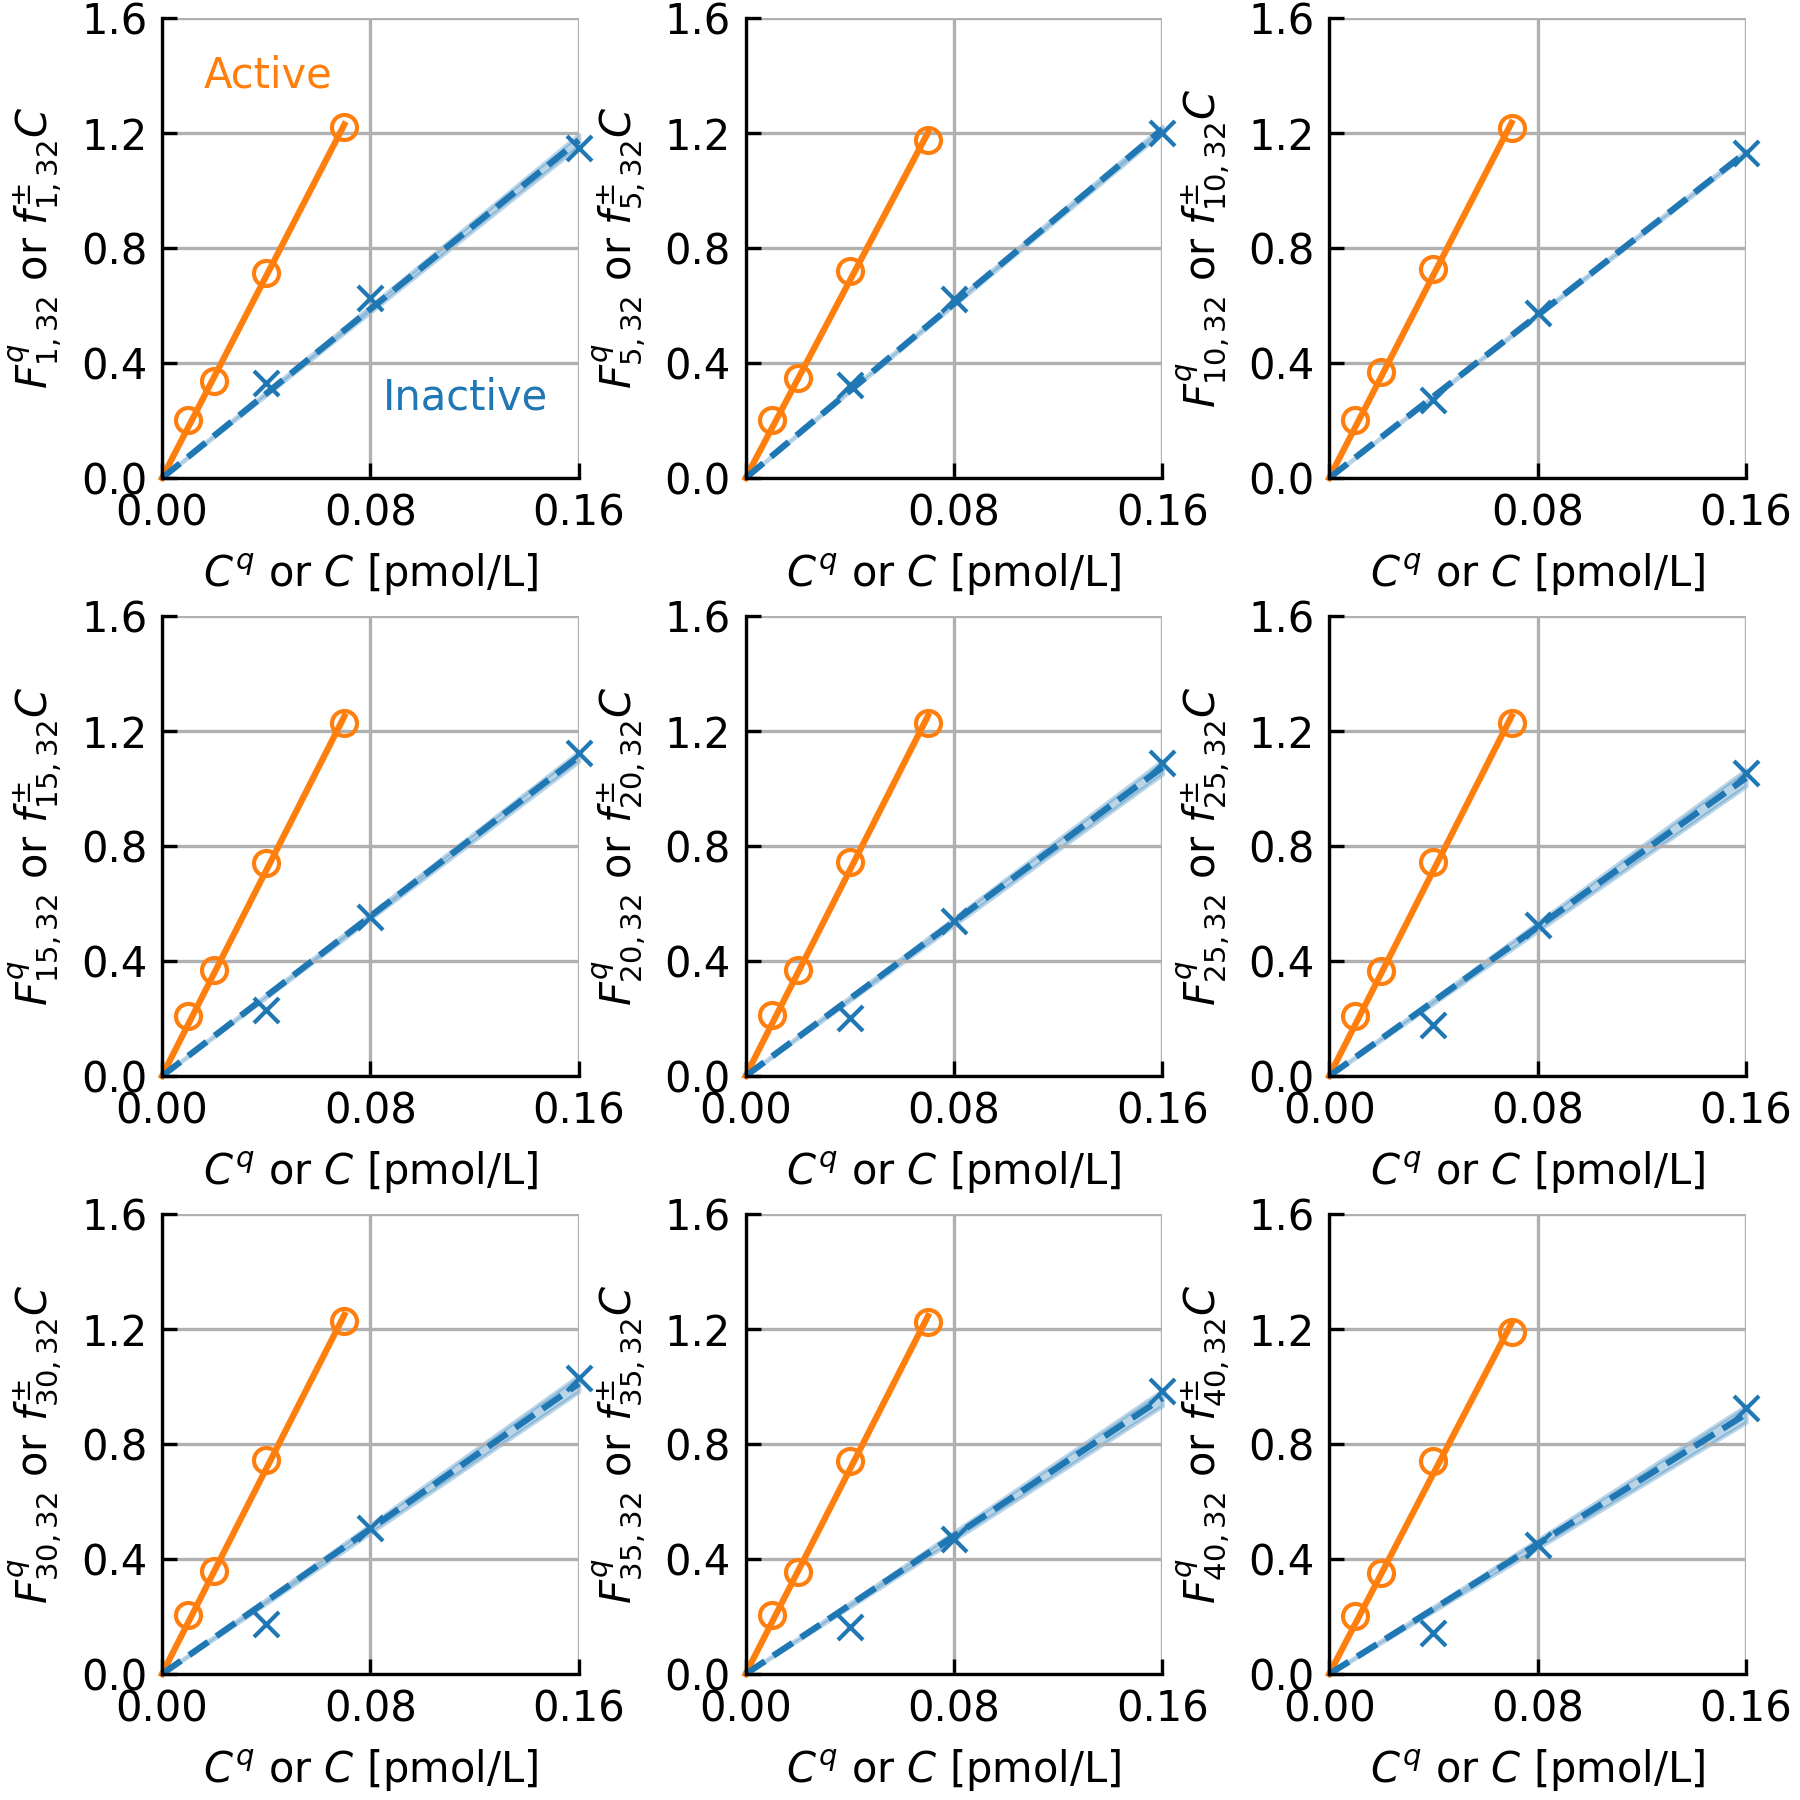
\includegraphics{si-figs/FigS32.png}
                    \caption{
                        As Figure~\ref{fig:S1} with well $w=32$ (or C8).
                    }
                \end{figure}
                \clearpage
    \begin{table}
        \caption{Molar Fluorescence Parameters for Well C8 ($w=32$)}
        \centering
        \begin{tabular}{c|ll|ll}
            Cycle & \multicolumn{2}{c|}{Inactive} & \multicolumn{2}{c}{Active} \\
            \hline
            $i$ & $f_{i,32}^{-}$ & $\sigma_{i,32}^{-}$ &  $f_{i,32}^{+}$ & $\sigma_{i,32}^{+}$ \\
            \hline
    1 & 7.34 & 0.042 & 17.57 & 0.019 \\
2 & 7.41 & 0.031 & 16.99 & 0.022 \\
3 & 7.69 & 0.023 & 17.20 & 0.026 \\
4 & 7.66 & 0.023 & 17.29 & 0.025 \\
5 & 7.58 & 0.021 & 17.16 & 0.030 \\
6 & 7.39 & 0.023 & 17.26 & 0.029 \\
7 & 7.32 & 0.016 & 17.41 & 0.026 \\
8 & 7.24 & 0.011 & 17.51 & 0.025 \\
9 & 7.155 & 0.0080 & 17.57 & 0.024 \\
10 & 7.08 & 0.011 & 17.65 & 0.024 \\
11 & 7.01 & 0.014 & 17.73 & 0.021 \\
12 & 6.98 & 0.019 & 17.75 & 0.021 \\
13 & 7.03 & 0.027 & 17.79 & 0.021 \\
14 & 6.99 & 0.031 & 17.84 & 0.025 \\
15 & 6.95 & 0.035 & 17.88 & 0.027 \\
16 & 6.89 & 0.037 & 17.90 & 0.027 \\
17 & 6.84 & 0.040 & 17.89 & 0.028 \\
18 & 6.81 & 0.044 & 17.90 & 0.028 \\
19 & 6.76 & 0.047 & 17.92 & 0.027 \\
20 & 6.71 & 0.049 & 17.90 & 0.029 \\
21 & 6.66 & 0.052 & 17.89 & 0.028 \\
22 & 6.61 & 0.054 & 17.89 & 0.028 \\
23 & 6.56 & 0.056 & 17.91 & 0.028 \\
24 & 6.54 & 0.059 & 17.89 & 0.028 \\
25 & 6.48 & 0.060 & 17.88 & 0.028 \\
26 & 6.43 & 0.054 & 17.88 & 0.028 \\
27 & 6.42 & 0.056 & 17.87 & 0.028 \\
28 & 6.39 & 0.057 & 17.91 & 0.027 \\
29 & 6.33 & 0.057 & 17.87 & 0.027 \\
30 & 6.31 & 0.058 & 17.85 & 0.027 \\
31 & 6.26 & 0.058 & 17.86 & 0.026 \\
32 & 6.24 & 0.059 & 17.80 & 0.026 \\
33 & 6.17 & 0.058 & 17.83 & 0.026 \\
34 & 6.04 & 0.058 & 17.79 & 0.026 \\
35 & 6.00 & 0.056 & 17.79 & 0.026 \\
36 & 5.95 & 0.048 & 17.90 & 0.023 \\
37 & 5.90 & 0.048 & 17.94 & 0.021 \\
38 & 5.83 & 0.045 & 17.68 & 0.028 \\
39 & 5.73 & 0.059 & 17.49 & 0.032 \\
40 & 5.65 & 0.060 & 17.43 & 0.034 \\
41 & 5.65 & 0.059 & 17.30 & 0.037 \\
42 & 5.61 & 0.059 & 17.19 & 0.043 \\
43 & 5.48 & 0.055 & 17.15 & 0.041 \\
44 & 5.32 & 0.070 & 17.03 & 0.044 \\
45 & 5.33 & 0.059 & 16.86 & 0.040 \\
               \hline
        \end{tabular}
    \end{table}
    \clearpage

                \begin{figure}
                    \centering
                    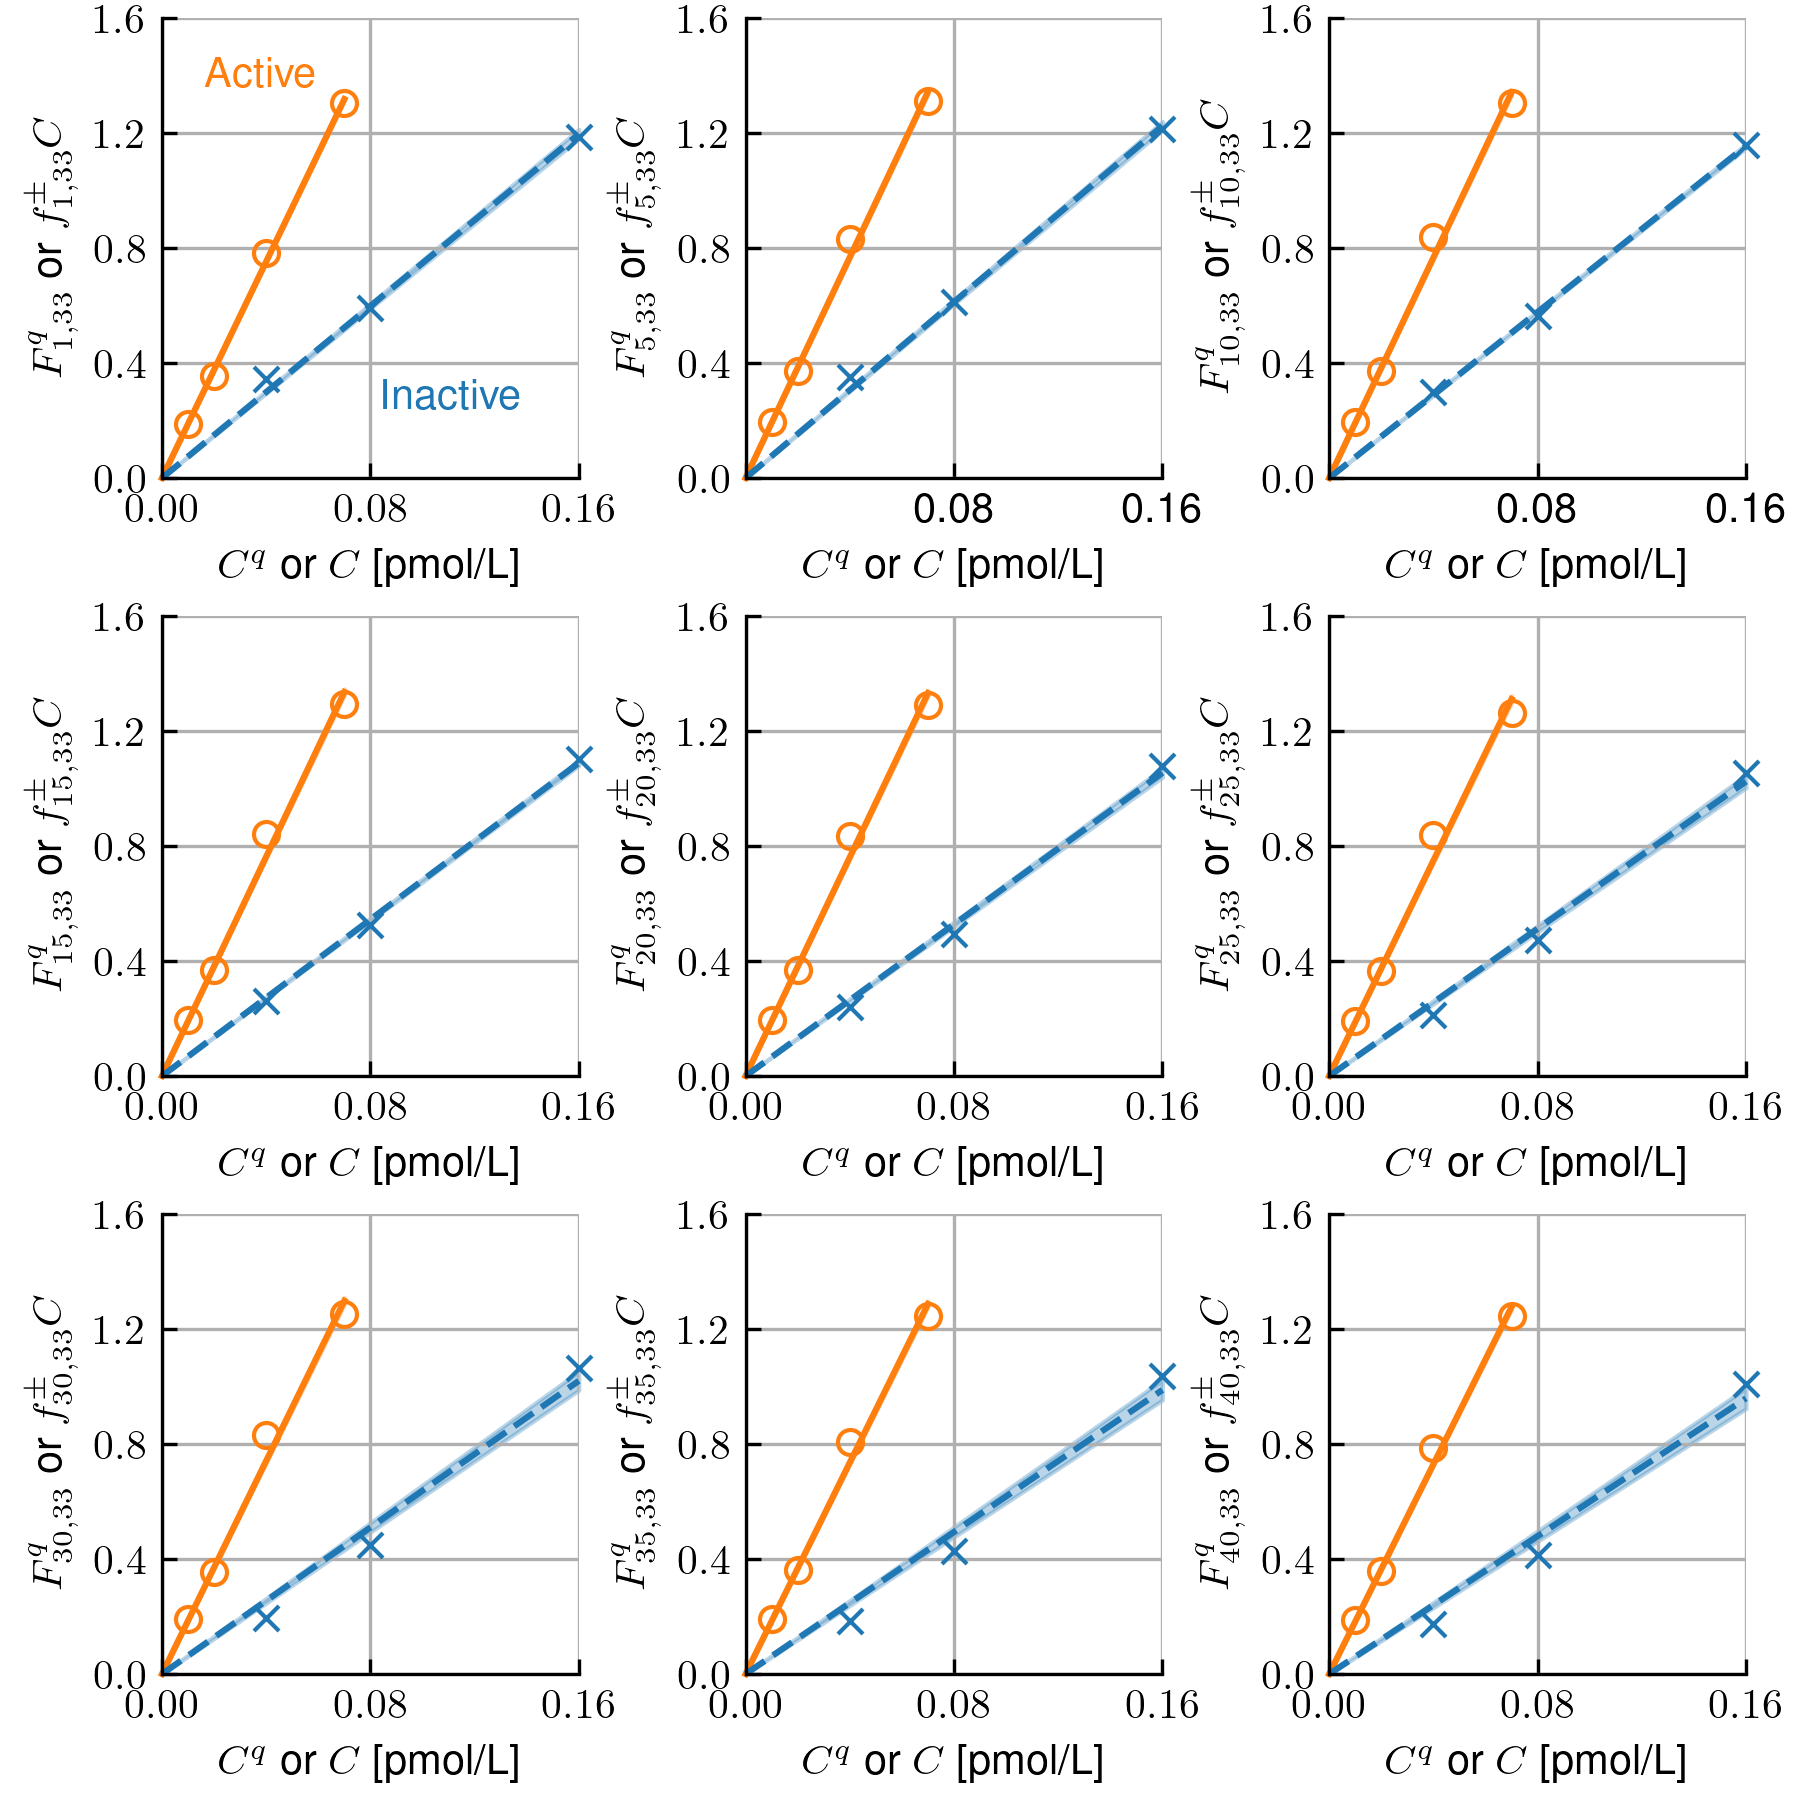
\includegraphics{si-figs/FigS33.png}
                    \caption{
                        As Figure~\ref{fig:S1} with well $w=33$ (or C9).
                    }
                \end{figure}
                \clearpage
    \begin{table}
        \caption{Molar Fluorescence Parameters for Well C9 ($w=33$)}
        \centering
        \begin{tabular}{c|ll|ll}
            Cycle & \multicolumn{2}{c|}{Inactive} & \multicolumn{2}{c}{Active} \\
            \hline
            $i$ & $f_{i,33}^{-}$ & $\sigma_{i,33}^{-}$ &  $f_{i,33}^{+}$ & $\sigma_{i,33}^{+}$ \\
            \hline
    1 & 7.48 & 0.034 & 18.82 & 0.023 \\
2 & 7.50 & 0.041 & 18.66 & 0.031 \\
3 & 7.66 & 0.038 & 18.97 & 0.038 \\
4 & 7.70 & 0.035 & 19.10 & 0.040 \\
5 & 7.65 & 0.032 & 19.19 & 0.041 \\
6 & 7.57 & 0.027 & 19.18 & 0.041 \\
7 & 7.48 & 0.022 & 19.19 & 0.044 \\
8 & 7.41 & 0.019 & 19.17 & 0.045 \\
9 & 7.31 & 0.016 & 19.15 & 0.048 \\
10 & 7.22 & 0.014 & 19.16 & 0.048 \\
11 & 7.13 & 0.015 & 19.14 & 0.049 \\
12 & 7.05 & 0.014 & 19.14 & 0.049 \\
13 & 6.99 & 0.016 & 19.10 & 0.051 \\
14 & 6.91 & 0.020 & 19.11 & 0.050 \\
15 & 6.81 & 0.019 & 19.08 & 0.052 \\
16 & 6.77 & 0.024 & 19.04 & 0.052 \\
17 & 6.70 & 0.020 & 19.03 & 0.053 \\
18 & 6.67 & 0.024 & 19.01 & 0.054 \\
19 & 6.72 & 0.035 & 19.00 & 0.054 \\
20 & 6.59 & 0.032 & 19.02 & 0.050 \\
21 & 6.56 & 0.031 & 18.97 & 0.053 \\
22 & 6.48 & 0.034 & 18.96 & 0.052 \\
23 & 6.46 & 0.038 & 18.94 & 0.053 \\
24 & 6.45 & 0.044 & 18.78 & 0.062 \\
25 & 6.40 & 0.046 & 18.73 & 0.059 \\
26 & 6.41 & 0.052 & 18.77 & 0.057 \\
27 & 6.36 & 0.051 & 18.67 & 0.059 \\
28 & 6.38 & 0.057 & 18.63 & 0.058 \\
29 & 6.39 & 0.063 & 18.56 & 0.057 \\
30 & 6.37 & 0.068 & 18.54 & 0.059 \\
31 & 6.34 & 0.070 & 18.59 & 0.061 \\
32 & 6.28 & 0.069 & 18.52 & 0.056 \\
33 & 6.20 & 0.067 & 18.37 & 0.050 \\
34 & 6.18 & 0.069 & 18.41 & 0.050 \\
35 & 6.17 & 0.073 & 18.38 & 0.049 \\
36 & 6.10 & 0.072 & 18.40 & 0.048 \\
37 & 6.06 & 0.071 & 18.40 & 0.048 \\
38 & 6.04 & 0.073 & 18.37 & 0.047 \\
39 & 6.04 & 0.075 & 18.38 & 0.045 \\
40 & 5.99 & 0.075 & 18.24 & 0.039 \\
41 & 5.94 & 0.074 & 18.20 & 0.044 \\
42 & 5.76 & 0.066 & 18.10 & 0.049 \\
43 & 5.78 & 0.070 & 17.82 & 0.056 \\
44 & 5.78 & 0.073 & 17.83 & 0.056 \\
45 & 5.76 & 0.073 & 17.83 & 0.055 \\
               \hline
        \end{tabular}
    \end{table}
    \clearpage

                \begin{figure}
                    \centering
                    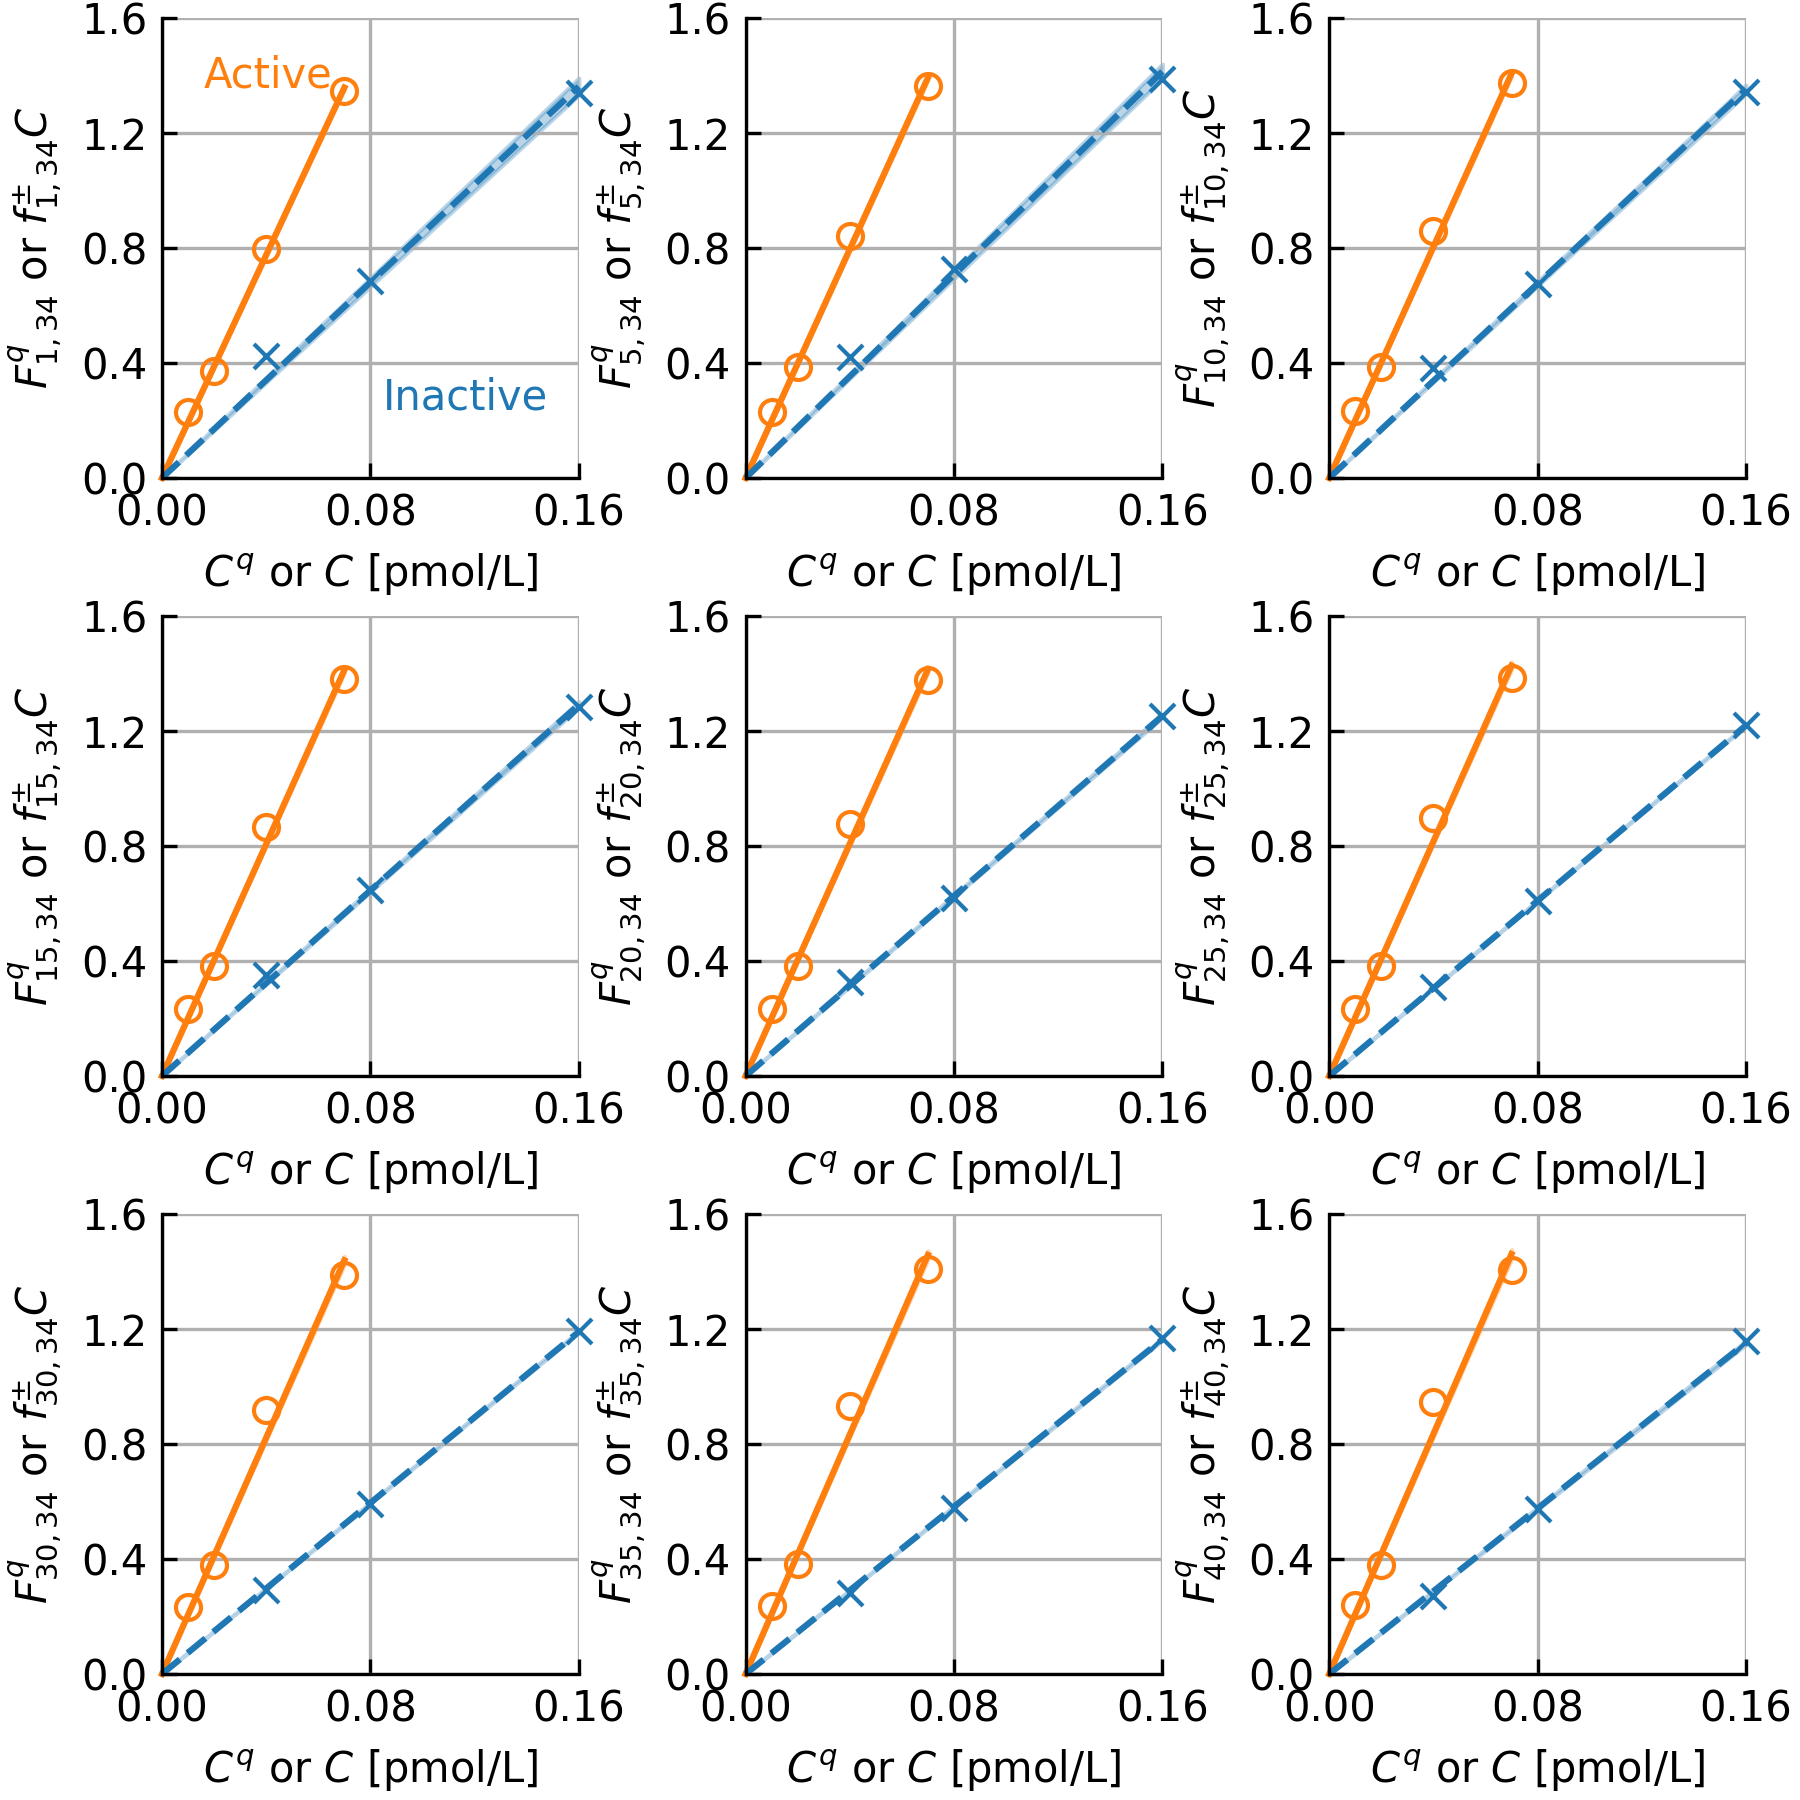
\includegraphics{si-figs/FigS34.png}
                    \caption{
                        As Figure~\ref{fig:S1} with well $w=34$ (or C10).
                    }
                \end{figure}
                \clearpage
    \begin{table}
        \caption{Molar Fluorescence Parameters for Well C10 ($w=34$)}
        \centering
        \begin{tabular}{c|ll|ll}
            Cycle & \multicolumn{2}{c|}{Inactive} & \multicolumn{2}{c}{Active} \\
            \hline
            $i$ & $f_{i,34}^{-}$ & $\sigma_{i,34}^{-}$ &  $f_{i,34}^{+}$ & $\sigma_{i,34}^{+}$ \\
            \hline
    1 & 8.51 & 0.061 & 19.40 & 0.026 \\
2 & 8.71 & 0.064 & 19.26 & 0.033 \\
3 & 8.86 & 0.061 & 19.64 & 0.034 \\
4 & 8.89 & 0.059 & 19.77 & 0.036 \\
5 & 8.84 & 0.054 & 19.89 & 0.037 \\
6 & 8.74 & 0.049 & 19.94 & 0.038 \\
7 & 8.66 & 0.044 & 20.03 & 0.040 \\
8 & 8.55 & 0.041 & 20.07 & 0.041 \\
9 & 8.50 & 0.036 & 20.10 & 0.041 \\
10 & 8.45 & 0.031 & 20.09 & 0.042 \\
11 & 8.33 & 0.030 & 20.12 & 0.041 \\
12 & 8.24 & 0.029 & 20.13 & 0.041 \\
13 & 8.16 & 0.027 & 20.14 & 0.044 \\
14 & 8.09 & 0.025 & 20.16 & 0.044 \\
15 & 8.07 & 0.021 & 20.17 & 0.043 \\
16 & 8.02 & 0.019 & 20.18 & 0.045 \\
17 & 7.98 & 0.016 & 20.19 & 0.045 \\
18 & 7.92 & 0.015 & 20.19 & 0.046 \\
19 & 7.90 & 0.013 & 20.18 & 0.047 \\
20 & 7.83 & 0.012 & 20.20 & 0.049 \\
21 & 7.803 & 0.0085 & 20.25 & 0.050 \\
22 & 7.756 & 0.0073 & 20.28 & 0.051 \\
23 & 7.710 & 0.0059 & 20.31 & 0.053 \\
24 & 7.684 & 0.0041 & 20.30 & 0.054 \\
25 & 7.622 & 0.0034 & 20.39 & 0.058 \\
26 & 7.585 & 0.0034 & 20.43 & 0.060 \\
27 & 7.540 & 0.0023 & 20.45 & 0.064 \\
28 & 7.508 & 0.0026 & 20.52 & 0.064 \\
29 & 7.470 & 0.0031 & 20.47 & 0.066 \\
30 & 7.441 & 0.0057 & 20.56 & 0.066 \\
31 & 7.402 & 0.0061 & 20.56 & 0.069 \\
32 & 7.362 & 0.0072 & 20.61 & 0.068 \\
33 & 7.332 & 0.0062 & 20.65 & 0.070 \\
34 & 7.303 & 0.0069 & 20.86 & 0.066 \\
35 & 7.274 & 0.0066 & 20.82 & 0.068 \\
36 & 7.218 & 0.0091 & 20.80 & 0.072 \\
37 & 7.25 & 0.011 & 20.88 & 0.072 \\
38 & 7.27 & 0.012 & 20.88 & 0.075 \\
39 & 7.24 & 0.011 & 20.89 & 0.076 \\
40 & 7.20 & 0.013 & 20.86 & 0.077 \\
41 & 7.19 & 0.014 & 20.87 & 0.080 \\
42 & 7.16 & 0.019 & 20.86 & 0.081 \\
43 & 7.15 & 0.020 & 20.92 & 0.082 \\
44 & 7.08 & 0.018 & 20.90 & 0.084 \\
45 & 7.08 & 0.019 & 20.96 & 0.085 \\
               \hline
        \end{tabular}
    \end{table}
    \clearpage

                \begin{figure}
                    \centering
                    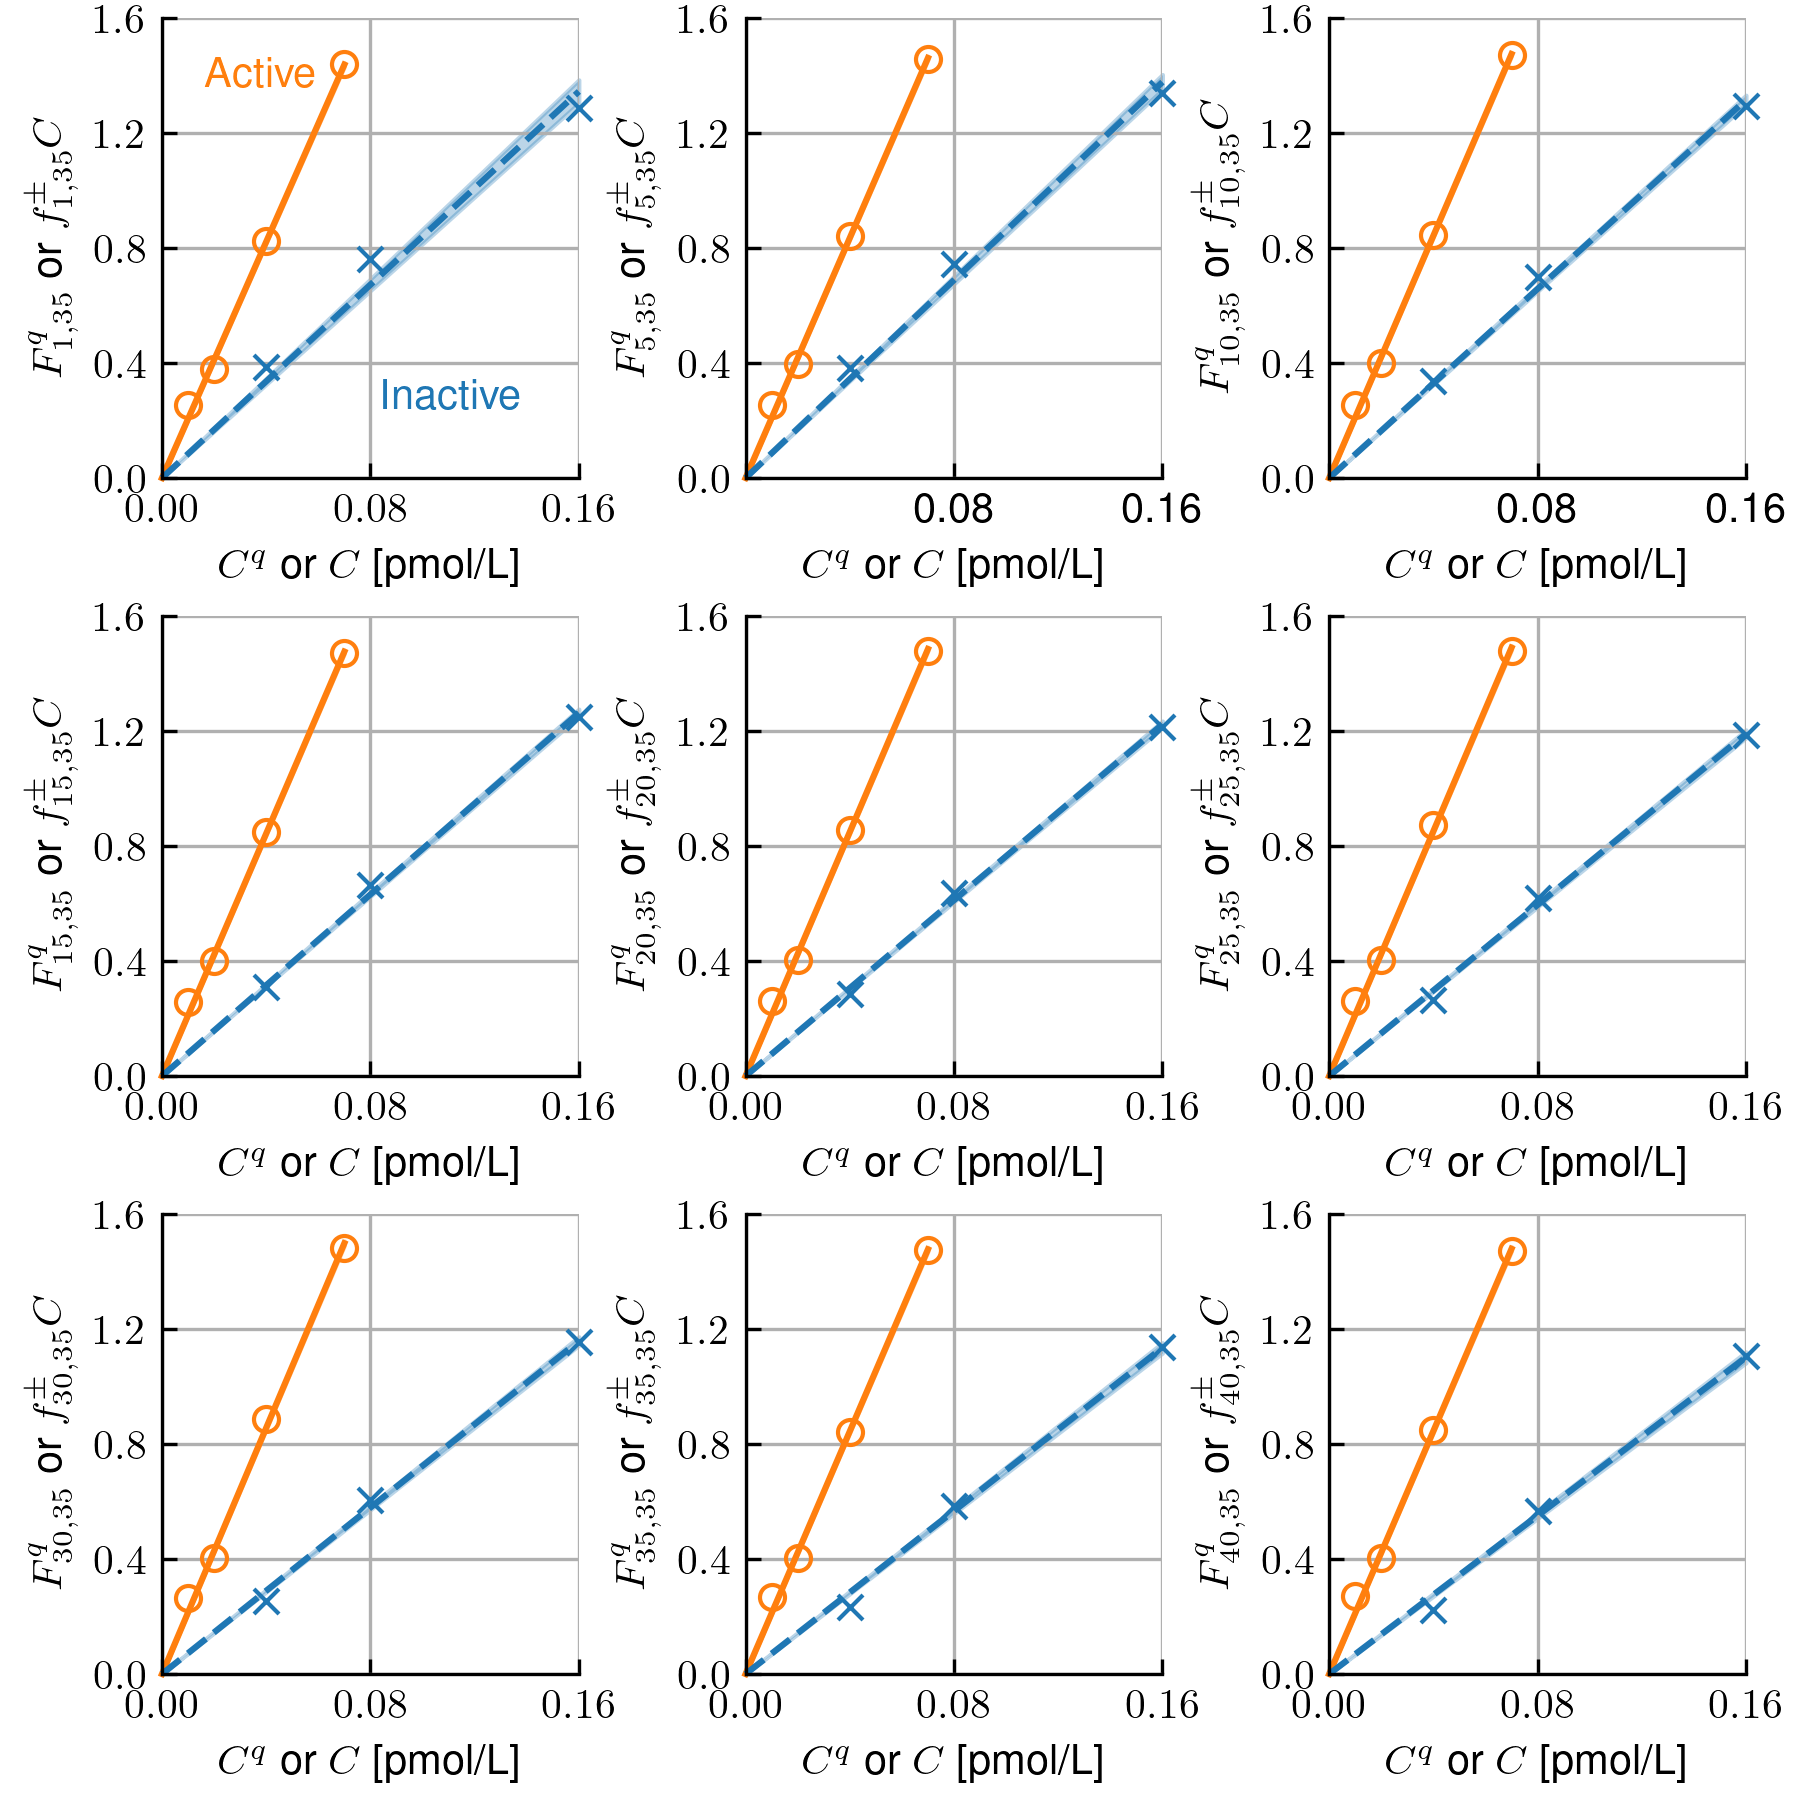
\includegraphics{si-figs/FigS35.png}
                    \caption{
                        As Figure~\ref{fig:S1} with well $w=35$ (or C11).
                    }
                \end{figure}
                \clearpage
    \begin{table}
        \caption{Molar Fluorescence Parameters for Well C11 ($w=35$)}
        \centering
        \begin{tabular}{c|ll|ll}
            Cycle & \multicolumn{2}{c|}{Inactive} & \multicolumn{2}{c}{Active} \\
            \hline
            $i$ & $f_{i,35}^{-}$ & $\sigma_{i,35}^{-}$ &  $f_{i,35}^{+}$ & $\sigma_{i,35}^{+}$ \\
            \hline
    1 & 8.40 & 0.084 & 20.54 & 0.033 \\
2 & 8.55 & 0.074 & 20.36 & 0.030 \\
3 & 8.69 & 0.066 & 20.62 & 0.029 \\
4 & 8.68 & 0.062 & 20.78 & 0.029 \\
5 & 8.61 & 0.055 & 20.87 & 0.029 \\
6 & 8.53 & 0.048 & 20.93 & 0.029 \\
7 & 8.46 & 0.043 & 20.98 & 0.029 \\
8 & 8.37 & 0.039 & 21.05 & 0.029 \\
9 & 8.30 & 0.036 & 21.06 & 0.029 \\
10 & 8.22 & 0.033 & 21.06 & 0.028 \\
11 & 8.15 & 0.032 & 21.13 & 0.028 \\
12 & 8.08 & 0.031 & 21.09 & 0.029 \\
13 & 8.01 & 0.029 & 21.12 & 0.029 \\
14 & 7.96 & 0.028 & 21.10 & 0.029 \\
15 & 7.90 & 0.027 & 21.08 & 0.029 \\
16 & 7.83 & 0.025 & 21.09 & 0.029 \\
17 & 7.78 & 0.026 & 21.09 & 0.029 \\
18 & 7.74 & 0.025 & 21.07 & 0.030 \\
19 & 7.68 & 0.024 & 21.20 & 0.031 \\
20 & 7.64 & 0.024 & 21.21 & 0.031 \\
21 & 7.64 & 0.024 & 21.18 & 0.032 \\
22 & 7.57 & 0.025 & 21.17 & 0.032 \\
23 & 7.52 & 0.026 & 21.21 & 0.032 \\
24 & 7.47 & 0.027 & 21.29 & 0.033 \\
25 & 7.44 & 0.028 & 21.28 & 0.035 \\
26 & 7.42 & 0.029 & 21.25 & 0.035 \\
27 & 7.36 & 0.029 & 21.26 & 0.036 \\
28 & 7.30 & 0.032 & 21.28 & 0.036 \\
29 & 7.25 & 0.033 & 21.30 & 0.036 \\
30 & 7.24 & 0.031 & 21.40 & 0.038 \\
31 & 7.23 & 0.033 & 21.37 & 0.037 \\
32 & 7.20 & 0.035 & 21.37 & 0.040 \\
33 & 7.16 & 0.034 & 21.22 & 0.036 \\
34 & 7.13 & 0.036 & 21.13 & 0.035 \\
35 & 7.09 & 0.037 & 21.10 & 0.035 \\
36 & 7.03 & 0.037 & 21.07 & 0.034 \\
37 & 6.98 & 0.038 & 21.12 & 0.035 \\
38 & 6.95 & 0.039 & 21.05 & 0.036 \\
39 & 6.91 & 0.040 & 21.29 & 0.036 \\
40 & 6.88 & 0.039 & 21.13 & 0.036 \\
41 & 6.87 & 0.039 & 21.02 & 0.038 \\
42 & 6.85 & 0.037 & 21.09 & 0.038 \\
43 & 6.84 & 0.039 & 21.05 & 0.039 \\
44 & 6.85 & 0.041 & 21.08 & 0.039 \\
45 & 6.92 & 0.043 & 21.04 & 0.040 \\
               \hline
        \end{tabular}
    \end{table}
    \clearpage

                \begin{figure}
                    \centering
                    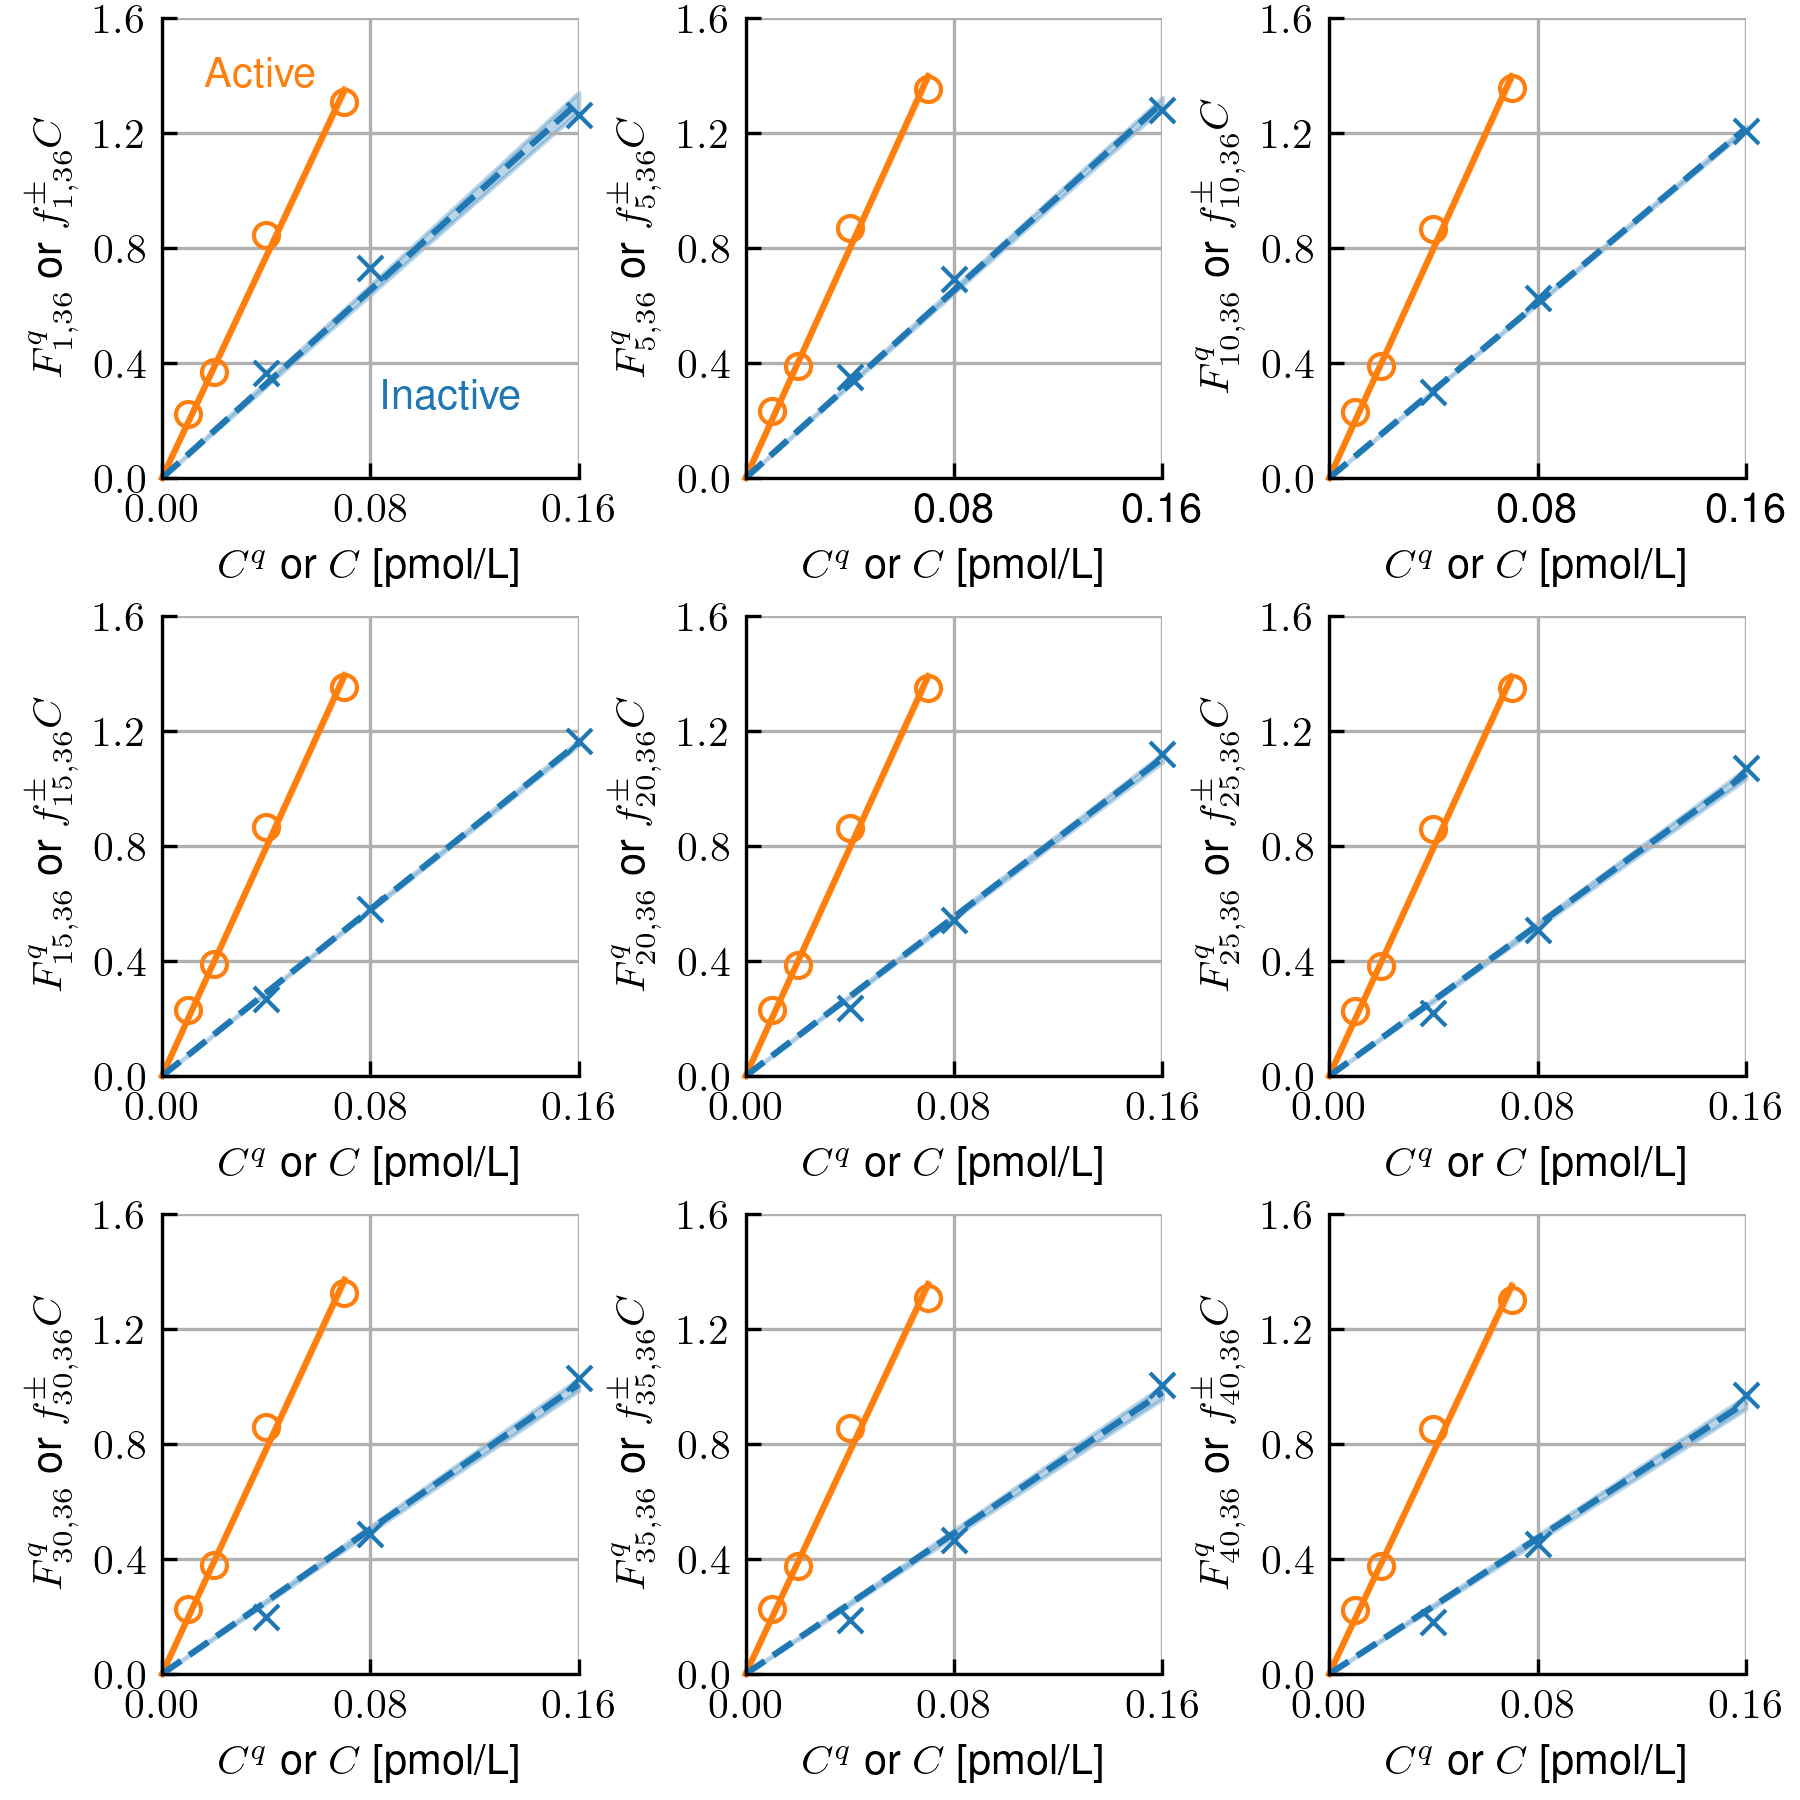
\includegraphics{si-figs/FigS36.png}
                    \caption{
                        As Figure~\ref{fig:S1} with well $w=36$ (or C12).
                    }
                \end{figure}
                \clearpage
    \begin{table}
        \caption{Molar Fluorescence Parameters for Well C12 ($w=36$)}
        \centering
        \begin{tabular}{c|ll|ll}
            Cycle & \multicolumn{2}{c|}{Inactive} & \multicolumn{2}{c}{Active} \\
            \hline
            $i$ & $f_{i,36}^{-}$ & $\sigma_{i,36}^{-}$ &  $f_{i,36}^{+}$ & $\sigma_{i,36}^{+}$ \\
            \hline
    1 & 8.18 & 0.069 & 19.27 & 0.053 \\
2 & 8.30 & 0.062 & 19.73 & 0.047 \\
3 & 8.38 & 0.054 & 19.86 & 0.051 \\
4 & 8.27 & 0.047 & 19.97 & 0.052 \\
5 & 8.16 & 0.038 & 19.96 & 0.053 \\
6 & 8.04 & 0.031 & 19.98 & 0.052 \\
7 & 7.91 & 0.026 & 19.97 & 0.052 \\
8 & 7.83 & 0.019 & 19.96 & 0.052 \\
9 & 7.72 & 0.016 & 19.94 & 0.052 \\
10 & 7.60 & 0.015 & 19.95 & 0.050 \\
11 & 7.52 & 0.013 & 19.94 & 0.052 \\
12 & 7.45 & 0.013 & 19.90 & 0.050 \\
13 & 7.37 & 0.014 & 19.90 & 0.051 \\
14 & 7.31 & 0.016 & 19.89 & 0.051 \\
15 & 7.24 & 0.017 & 19.90 & 0.050 \\
16 & 7.18 & 0.018 & 19.88 & 0.048 \\
17 & 7.10 & 0.022 & 19.93 & 0.051 \\
18 & 7.01 & 0.023 & 19.88 & 0.051 \\
19 & 6.98 & 0.025 & 19.87 & 0.050 \\
20 & 6.91 & 0.030 & 19.85 & 0.049 \\
21 & 6.85 & 0.033 & 19.85 & 0.050 \\
22 & 6.74 & 0.035 & 19.86 & 0.051 \\
23 & 6.67 & 0.037 & 19.86 & 0.046 \\
24 & 6.64 & 0.039 & 19.85 & 0.048 \\
25 & 6.57 & 0.036 & 19.84 & 0.048 \\
26 & 6.53 & 0.043 & 19.72 & 0.051 \\
27 & 6.50 & 0.043 & 19.71 & 0.050 \\
28 & 6.44 & 0.046 & 19.80 & 0.050 \\
29 & 6.39 & 0.045 & 19.79 & 0.049 \\
30 & 6.29 & 0.043 & 19.57 & 0.055 \\
31 & 6.27 & 0.045 & 19.58 & 0.054 \\
32 & 6.21 & 0.048 & 19.57 & 0.054 \\
33 & 6.17 & 0.046 & 19.43 & 0.058 \\
34 & 6.11 & 0.042 & 19.40 & 0.058 \\
35 & 6.12 & 0.047 & 19.36 & 0.058 \\
36 & 6.07 & 0.046 & 19.40 & 0.057 \\
37 & 6.02 & 0.047 & 19.46 & 0.057 \\
38 & 5.98 & 0.046 & 19.37 & 0.057 \\
39 & 5.99 & 0.049 & 19.32 & 0.057 \\
40 & 5.90 & 0.046 & 19.28 & 0.058 \\
41 & 5.88 & 0.046 & 19.15 & 0.063 \\
42 & 5.84 & 0.045 & 19.25 & 0.060 \\
43 & 5.81 & 0.045 & 19.16 & 0.060 \\
44 & 5.77 & 0.044 & 19.19 & 0.058 \\
45 & 5.73 & 0.045 & 18.95 & 0.044 \\
               \hline
        \end{tabular}
    \end{table}
    \clearpage

                \begin{figure}
                    \centering
                    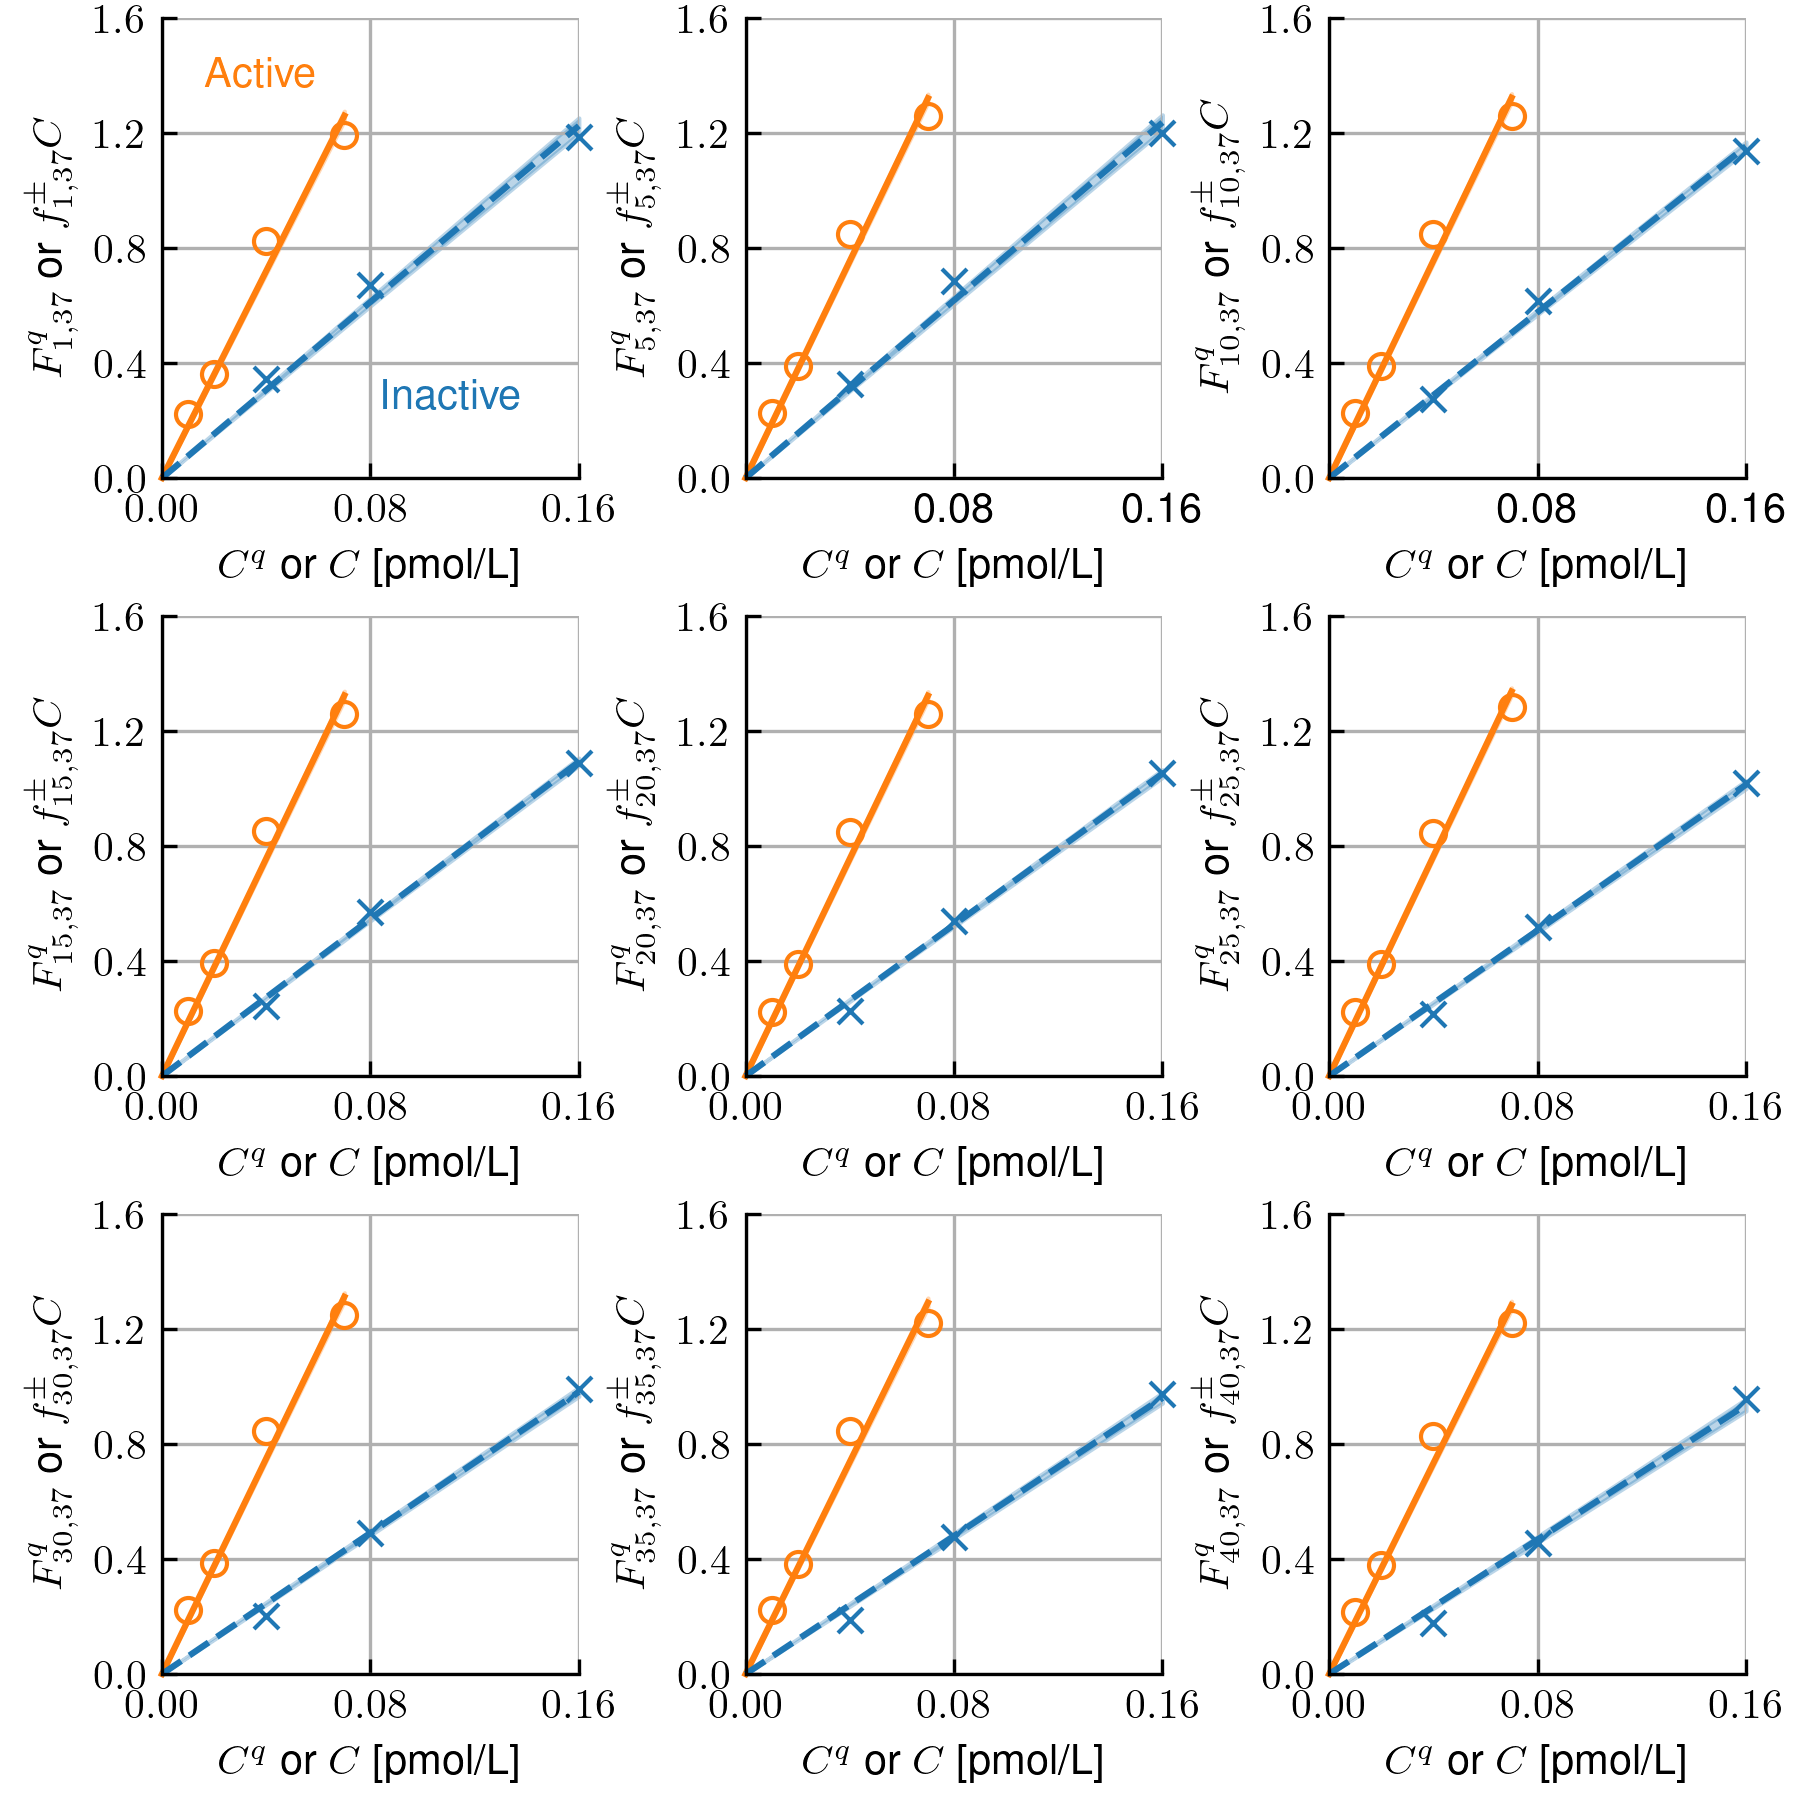
\includegraphics{si-figs/FigS37.png}
                    \caption{
                        As Figure~\ref{fig:S1} with well $w=37$ (or D1).
                    }
                \end{figure}
                \clearpage
    \begin{table}
        \caption{Molar Fluorescence Parameters for Well D1 ($w=37$)}
        \centering
        \begin{tabular}{c|ll|ll}
            Cycle & \multicolumn{2}{c|}{Inactive} & \multicolumn{2}{c}{Active} \\
            \hline
            $i$ & $f_{i,37}^{-}$ & $\sigma_{i,37}^{-}$ &  $f_{i,37}^{+}$ & $\sigma_{i,37}^{+}$ \\
            \hline
    1 & 7.66 & 0.057 & 18.00 & 0.076 \\
2 & 7.93 & 0.062 & 18.47 & 0.067 \\
3 & 7.96 & 0.065 & 18.69 & 0.069 \\
4 & 7.86 & 0.061 & 18.78 & 0.069 \\
5 & 7.73 & 0.056 & 18.87 & 0.069 \\
6 & 7.61 & 0.048 & 18.86 & 0.069 \\
7 & 7.50 & 0.042 & 18.89 & 0.069 \\
8 & 7.39 & 0.039 & 18.87 & 0.069 \\
9 & 7.30 & 0.034 & 18.89 & 0.069 \\
10 & 7.21 & 0.032 & 18.89 & 0.069 \\
11 & 7.13 & 0.030 & 18.89 & 0.070 \\
12 & 7.05 & 0.029 & 18.91 & 0.070 \\
13 & 6.99 & 0.028 & 18.92 & 0.071 \\
14 & 6.88 & 0.028 & 18.90 & 0.070 \\
15 & 6.83 & 0.027 & 18.91 & 0.071 \\
16 & 6.79 & 0.028 & 18.89 & 0.071 \\
17 & 6.70 & 0.028 & 18.88 & 0.071 \\
18 & 6.65 & 0.028 & 18.90 & 0.072 \\
19 & 6.61 & 0.027 & 18.86 & 0.073 \\
20 & 6.58 & 0.028 & 18.90 & 0.068 \\
21 & 6.58 & 0.030 & 18.83 & 0.069 \\
22 & 6.59 & 0.031 & 18.85 & 0.070 \\
23 & 6.50 & 0.030 & 18.84 & 0.073 \\
24 & 6.40 & 0.029 & 18.85 & 0.069 \\
25 & 6.33 & 0.029 & 19.11 & 0.060 \\
26 & 6.29 & 0.028 & 18.89 & 0.065 \\
27 & 6.25 & 0.028 & 18.86 & 0.065 \\
28 & 6.21 & 0.030 & 18.80 & 0.066 \\
29 & 6.18 & 0.031 & 18.75 & 0.068 \\
30 & 6.13 & 0.032 & 18.74 & 0.068 \\
31 & 6.10 & 0.033 & 18.83 & 0.066 \\
32 & 6.07 & 0.034 & 18.42 & 0.077 \\
33 & 6.04 & 0.035 & 18.44 & 0.077 \\
34 & 6.00 & 0.036 & 18.47 & 0.076 \\
35 & 6.00 & 0.037 & 18.45 & 0.078 \\
36 & 5.96 & 0.039 & 18.41 & 0.071 \\
37 & 5.95 & 0.039 & 18.37 & 0.070 \\
38 & 5.89 & 0.041 & 18.38 & 0.068 \\
39 & 5.87 & 0.043 & 18.32 & 0.069 \\
40 & 5.85 & 0.043 & 18.32 & 0.068 \\
41 & 5.82 & 0.045 & 18.37 & 0.065 \\
42 & 5.80 & 0.046 & 18.32 & 0.066 \\
43 & 5.80 & 0.048 & 18.27 & 0.068 \\
44 & 5.75 & 0.048 & 18.26 & 0.067 \\
45 & 5.73 & 0.049 & 18.09 & 0.073 \\
               \hline
        \end{tabular}
    \end{table}
    \clearpage

                \begin{figure}
                    \centering
                    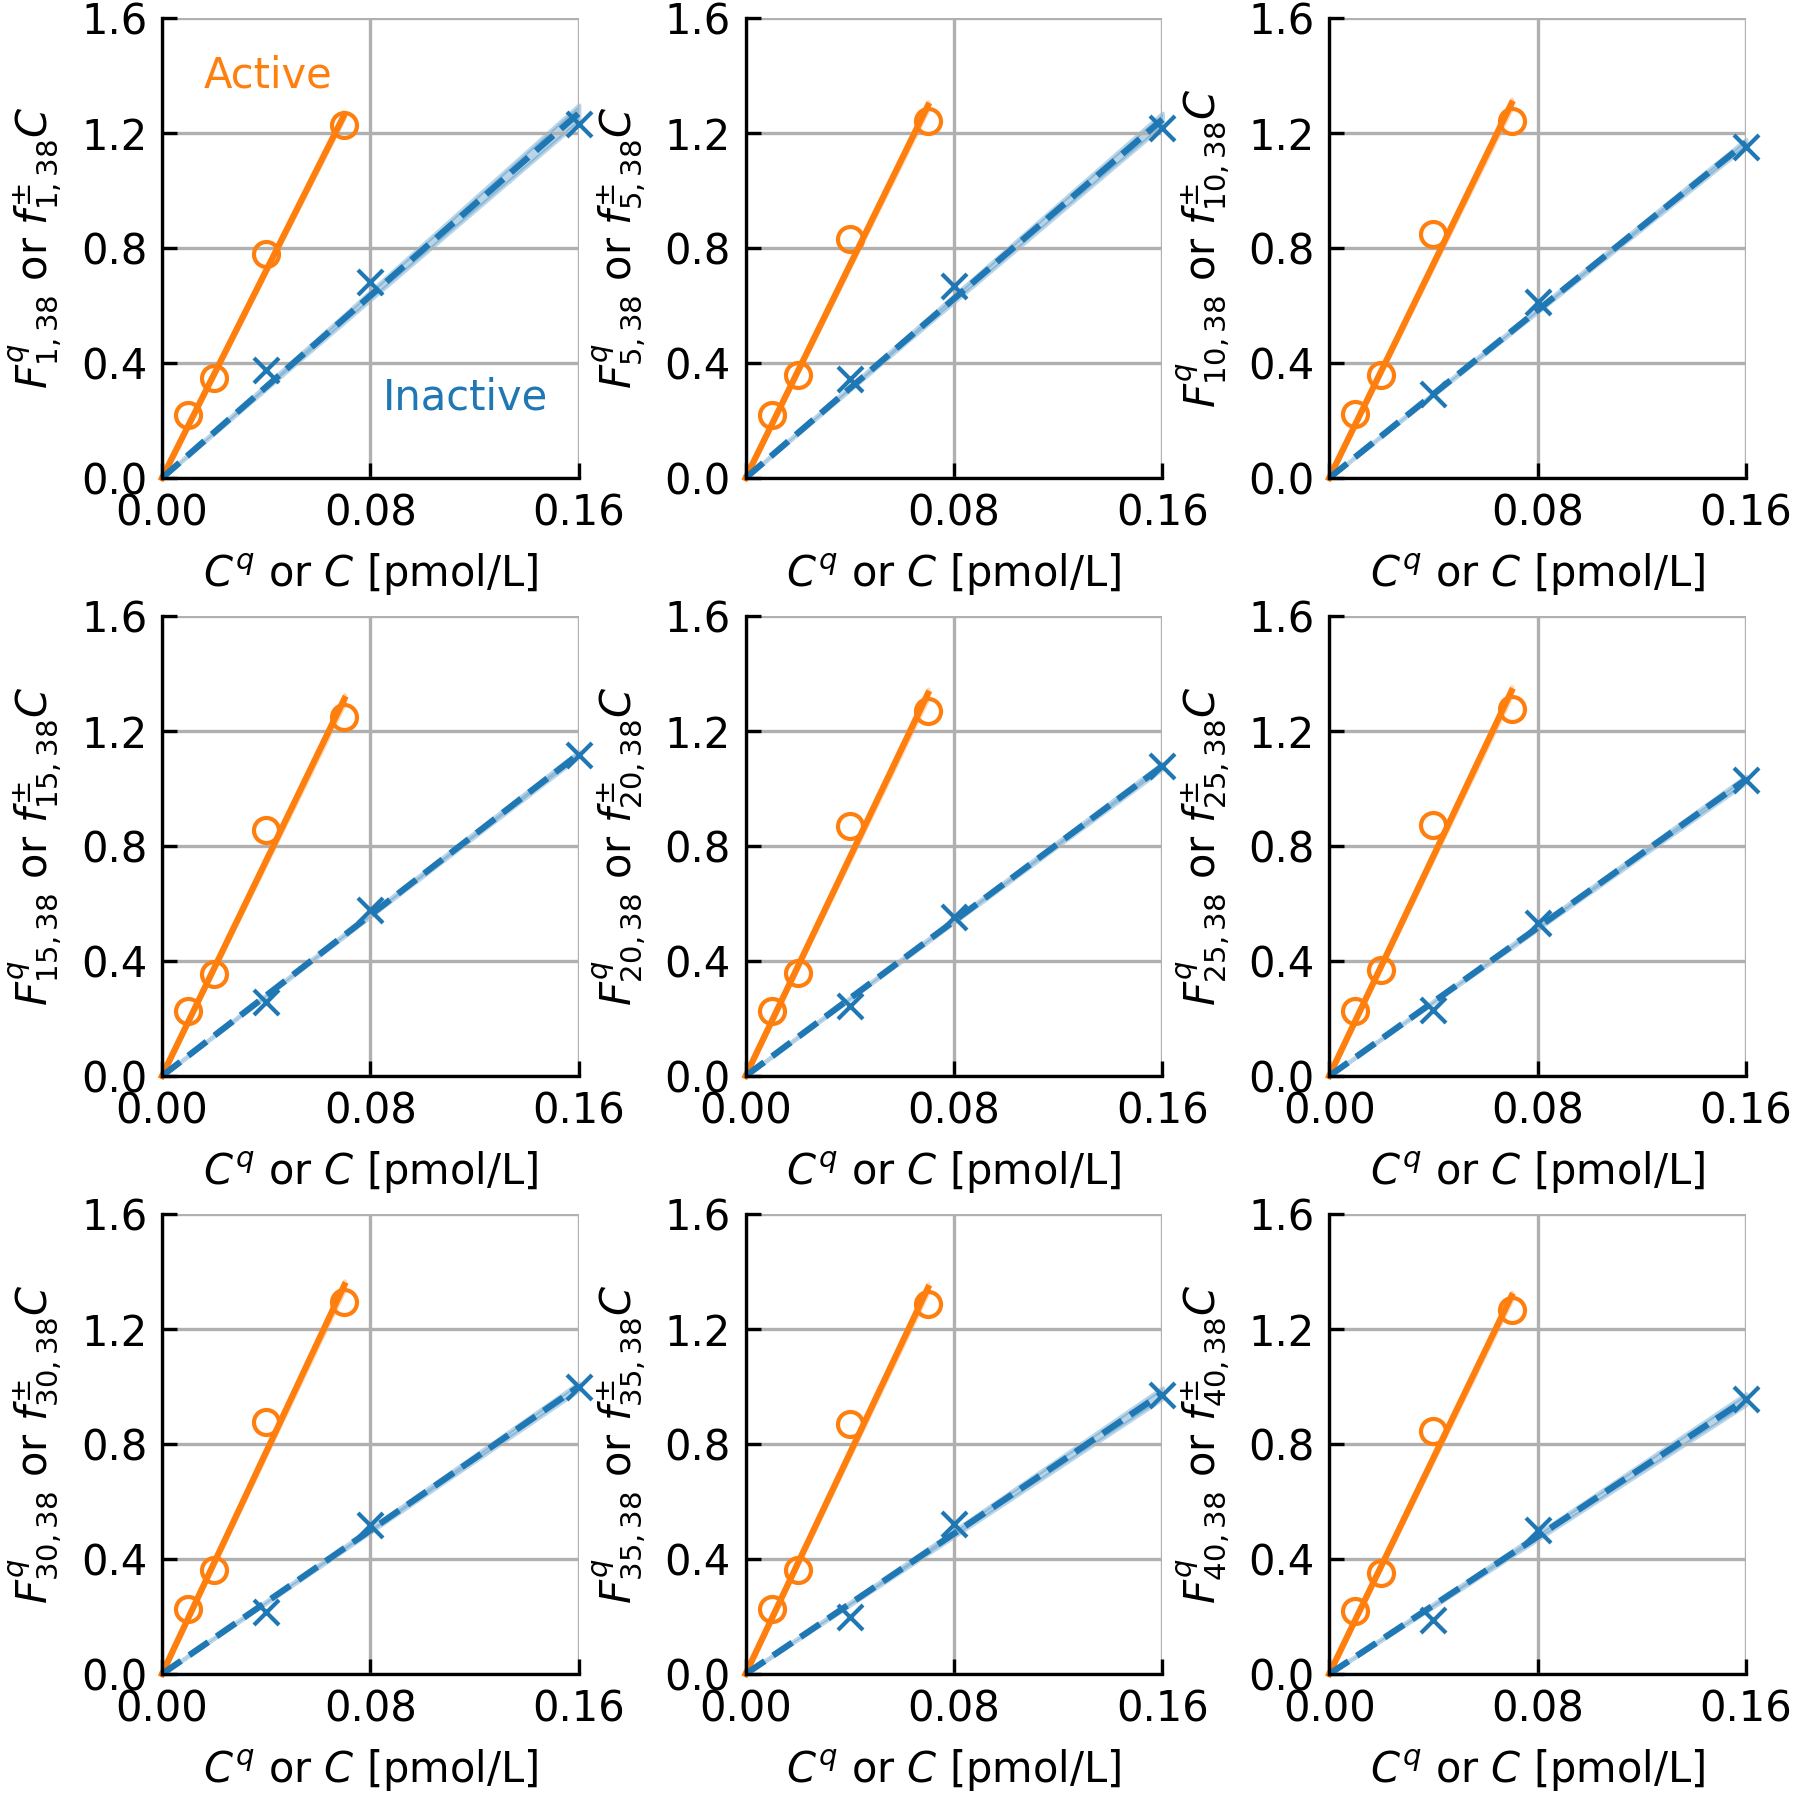
\includegraphics{si-figs/FigS38.png}
                    \caption{
                        As Figure~\ref{fig:S1} with well $w=38$ (or D2).
                    }
                \end{figure}
                \clearpage
    \begin{table}
        \caption{Molar Fluorescence Parameters for Well D2 ($w=38$)}
        \centering
        \begin{tabular}{c|ll|ll}
            Cycle & \multicolumn{2}{c|}{Inactive} & \multicolumn{2}{c}{Active} \\
            \hline
            $i$ & $f_{i,38}^{-}$ & $\sigma_{i,38}^{-}$ &  $f_{i,38}^{+}$ & $\sigma_{i,38}^{+}$ \\
            \hline
    1 & 7.93 & 0.059 & 18.05 & 0.046 \\
2 & 8.06 & 0.058 & 18.09 & 0.057 \\
3 & 8.09 & 0.055 & 18.28 & 0.063 \\
4 & 7.94 & 0.052 & 18.44 & 0.065 \\
5 & 7.79 & 0.046 & 18.50 & 0.065 \\
6 & 7.69 & 0.038 & 18.51 & 0.068 \\
7 & 7.59 & 0.032 & 18.54 & 0.069 \\
8 & 7.49 & 0.027 & 18.59 & 0.069 \\
9 & 7.39 & 0.025 & 18.60 & 0.072 \\
10 & 7.29 & 0.024 & 18.61 & 0.074 \\
11 & 7.20 & 0.019 & 18.62 & 0.074 \\
12 & 7.14 & 0.018 & 18.59 & 0.076 \\
13 & 7.07 & 0.019 & 18.65 & 0.075 \\
14 & 7.02 & 0.019 & 18.71 & 0.076 \\
15 & 7.00 & 0.020 & 18.73 & 0.075 \\
16 & 6.95 & 0.020 & 18.78 & 0.075 \\
17 & 6.87 & 0.024 & 18.82 & 0.075 \\
18 & 6.81 & 0.023 & 18.91 & 0.074 \\
19 & 6.84 & 0.023 & 18.97 & 0.076 \\
20 & 6.74 & 0.021 & 19.00 & 0.077 \\
21 & 6.66 & 0.027 & 19.03 & 0.075 \\
22 & 6.60 & 0.026 & 19.06 & 0.074 \\
23 & 6.54 & 0.025 & 19.02 & 0.076 \\
24 & 6.50 & 0.024 & 19.03 & 0.076 \\
25 & 6.45 & 0.023 & 19.13 & 0.074 \\
26 & 6.47 & 0.026 & 19.15 & 0.076 \\
27 & 6.38 & 0.028 & 19.20 & 0.074 \\
28 & 6.32 & 0.027 & 19.21 & 0.075 \\
29 & 6.28 & 0.026 & 19.24 & 0.074 \\
30 & 6.25 & 0.027 & 19.32 & 0.073 \\
31 & 6.20 & 0.029 & 19.27 & 0.074 \\
32 & 6.15 & 0.031 & 19.26 & 0.076 \\
33 & 6.12 & 0.034 & 19.22 & 0.072 \\
34 & 6.11 & 0.035 & 19.19 & 0.070 \\
35 & 6.10 & 0.040 & 19.18 & 0.071 \\
36 & 6.06 & 0.037 & 19.20 & 0.070 \\
37 & 6.03 & 0.037 & 19.10 & 0.066 \\
38 & 6.02 & 0.038 & 18.88 & 0.074 \\
39 & 5.98 & 0.038 & 18.87 & 0.074 \\
40 & 5.97 & 0.040 & 18.78 & 0.065 \\
41 & 5.97 & 0.040 & 18.81 & 0.066 \\
42 & 5.95 & 0.041 & 18.80 & 0.067 \\
43 & 5.94 & 0.042 & 18.77 & 0.068 \\
44 & 5.92 & 0.043 & 18.67 & 0.072 \\
45 & 5.89 & 0.045 & 18.71 & 0.071 \\
               \hline
        \end{tabular}
    \end{table}
    \clearpage

                \begin{figure}
                    \centering
                    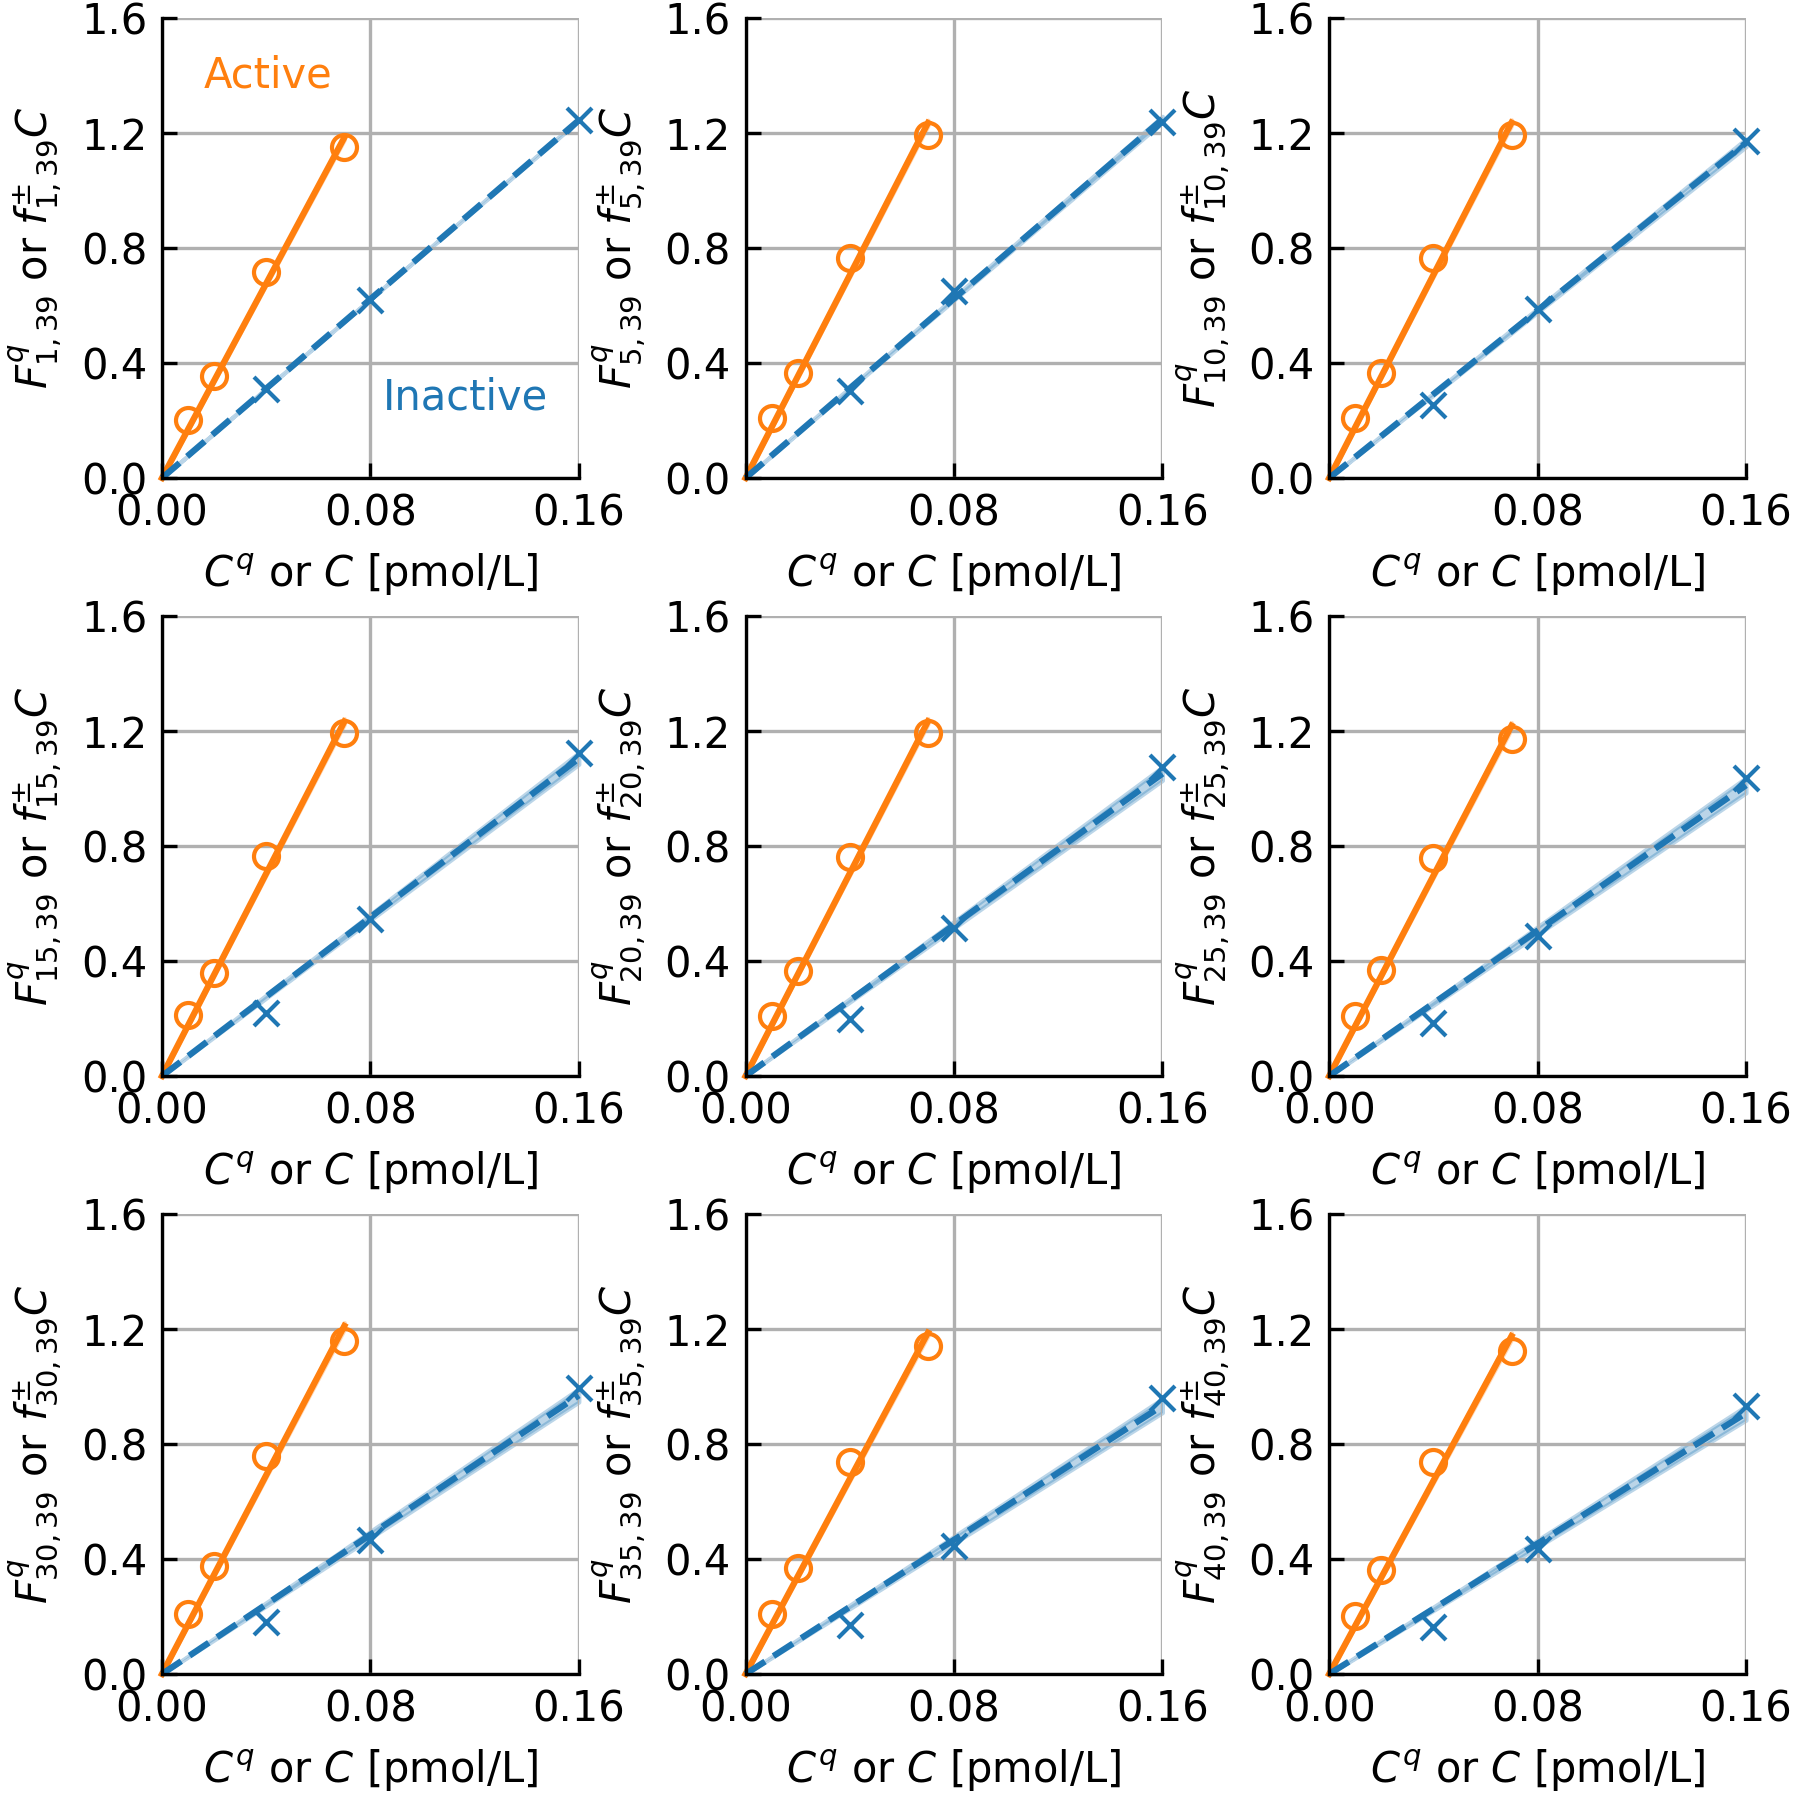
\includegraphics{si-figs/FigS39.png}
                    \caption{
                        As Figure~\ref{fig:S1} with well $w=39$ (or D3).
                    }
                \end{figure}
                \clearpage
    \begin{table}
        \caption{Molar Fluorescence Parameters for Well D3 ($w=39$)}
        \centering
        \begin{tabular}{c|ll|ll}
            Cycle & \multicolumn{2}{c|}{Inactive} & \multicolumn{2}{c}{Active} \\
            \hline
            $i$ & $f_{i,39}^{-}$ & $\sigma_{i,39}^{-}$ &  $f_{i,39}^{+}$ & $\sigma_{i,39}^{+}$ \\
            \hline
    1 & 7.779 & 0.0033 & 16.92 & 0.037 \\
2 & 7.91 & 0.018 & 17.20 & 0.040 \\
3 & 7.99 & 0.022 & 17.43 & 0.043 \\
4 & 7.92 & 0.023 & 17.56 & 0.046 \\
5 & 7.80 & 0.021 & 17.64 & 0.046 \\
6 & 7.69 & 0.019 & 17.69 & 0.046 \\
7 & 7.58 & 0.020 & 17.71 & 0.045 \\
8 & 7.48 & 0.022 & 17.66 & 0.047 \\
9 & 7.38 & 0.026 & 17.68 & 0.046 \\
10 & 7.29 & 0.028 & 17.66 & 0.047 \\
11 & 7.20 & 0.032 & 17.65 & 0.046 \\
12 & 7.12 & 0.035 & 17.64 & 0.047 \\
13 & 7.04 & 0.037 & 17.64 & 0.047 \\
14 & 6.97 & 0.040 & 17.64 & 0.047 \\
15 & 6.90 & 0.042 & 17.62 & 0.046 \\
16 & 6.83 & 0.044 & 17.65 & 0.045 \\
17 & 6.74 & 0.045 & 17.64 & 0.045 \\
18 & 6.68 & 0.046 & 17.64 & 0.045 \\
19 & 6.63 & 0.047 & 17.64 & 0.044 \\
20 & 6.57 & 0.049 & 17.63 & 0.046 \\
21 & 6.51 & 0.050 & 17.66 & 0.046 \\
22 & 6.46 & 0.051 & 17.60 & 0.046 \\
23 & 6.47 & 0.055 & 17.54 & 0.048 \\
24 & 6.39 & 0.055 & 17.41 & 0.051 \\
25 & 6.32 & 0.055 & 17.41 & 0.051 \\
26 & 6.33 & 0.058 & 17.36 & 0.053 \\
27 & 6.22 & 0.049 & 17.37 & 0.053 \\
28 & 6.16 & 0.046 & 17.32 & 0.054 \\
29 & 6.13 & 0.048 & 17.28 & 0.054 \\
30 & 6.06 & 0.048 & 17.30 & 0.055 \\
31 & 6.01 & 0.047 & 17.48 & 0.050 \\
32 & 5.97 & 0.048 & 17.32 & 0.052 \\
33 & 5.94 & 0.048 & 17.25 & 0.053 \\
34 & 5.89 & 0.049 & 17.20 & 0.056 \\
35 & 5.83 & 0.050 & 16.96 & 0.052 \\
36 & 5.81 & 0.050 & 17.01 & 0.052 \\
37 & 5.79 & 0.051 & 16.96 & 0.053 \\
38 & 5.73 & 0.051 & 16.93 & 0.054 \\
39 & 5.69 & 0.051 & 16.89 & 0.055 \\
40 & 5.67 & 0.051 & 16.79 & 0.054 \\
41 & 5.68 & 0.054 & 16.79 & 0.054 \\
42 & 5.60 & 0.054 & 16.70 & 0.058 \\
43 & 5.53 & 0.051 & 16.73 & 0.057 \\
44 & 5.52 & 0.053 & 16.66 & 0.057 \\
45 & 5.48 & 0.053 & 16.65 & 0.057 \\
               \hline
        \end{tabular}
    \end{table}
    \clearpage

                \begin{figure}
                    \centering
                    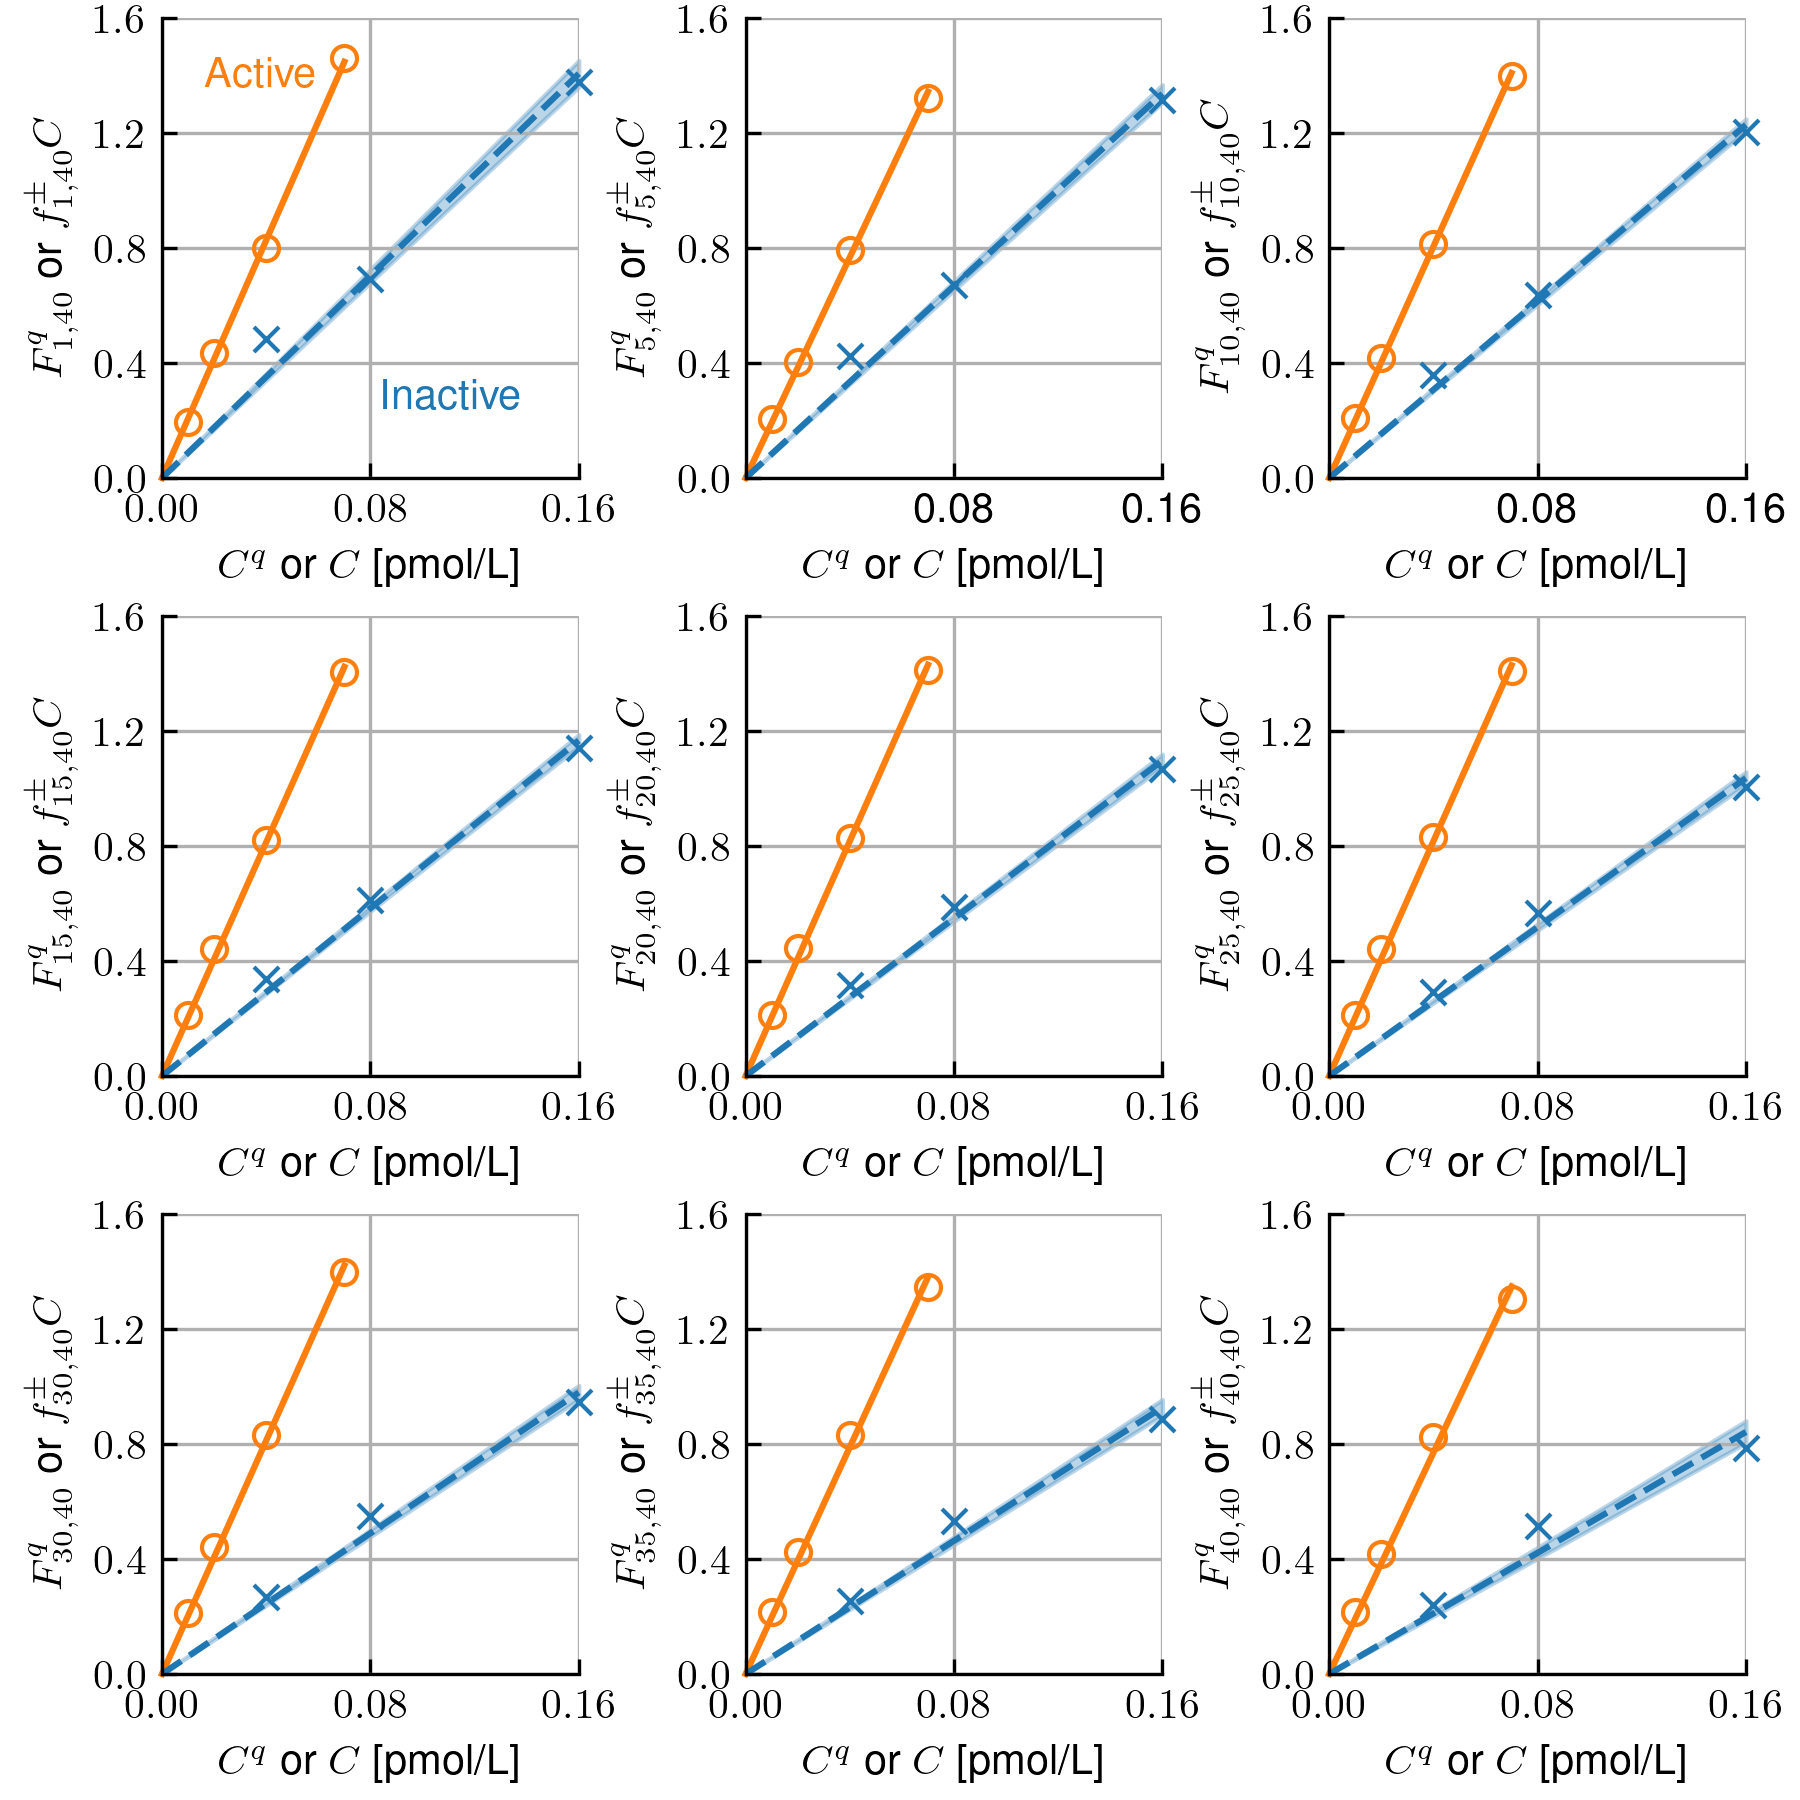
\includegraphics{si-figs/FigS40.png}
                    \caption{
                        As Figure~\ref{fig:S1} with well $w=40$ (or D4).
                    }
                \end{figure}
                \clearpage
    \begin{table}
        \caption{Molar Fluorescence Parameters for Well D4 ($w=40$)}
        \centering
        \begin{tabular}{c|ll|ll}
            Cycle & \multicolumn{2}{c|}{Inactive} & \multicolumn{2}{c}{Active} \\
            \hline
            $i$ & $f_{i,40}^{-}$ & $\sigma_{i,40}^{-}$ &  $f_{i,40}^{+}$ & $\sigma_{i,40}^{+}$ \\
            \hline
    1 & 8.79 & 0.096 & 20.68 & 0.022 \\
2 & 8.42 & 0.074 & 19.53 & 0.011 \\
3 & 8.54 & 0.069 & 19.41 & 0.013 \\
4 & 8.49 & 0.069 & 19.39 & 0.016 \\
5 & 8.36 & 0.065 & 19.20 & 0.024 \\
6 & 8.21 & 0.060 & 19.35 & 0.022 \\
7 & 8.05 & 0.054 & 19.71 & 0.014 \\
8 & 7.92 & 0.051 & 19.92 & 0.010 \\
9 & 7.80 & 0.047 & 20.031 & 0.0096 \\
10 & 7.68 & 0.044 & 20.13 & 0.013 \\
11 & 7.54 & 0.032 & 20.21 & 0.014 \\
12 & 7.45 & 0.039 & 20.27 & 0.017 \\
13 & 7.38 & 0.049 & 20.30 & 0.020 \\
14 & 7.35 & 0.045 & 20.32 & 0.022 \\
15 & 7.29 & 0.043 & 20.33 & 0.024 \\
16 & 7.21 & 0.042 & 20.35 & 0.019 \\
17 & 7.12 & 0.042 & 20.35 & 0.022 \\
18 & 7.03 & 0.043 & 20.39 & 0.023 \\
19 & 6.95 & 0.044 & 20.42 & 0.025 \\
20 & 6.86 & 0.046 & 20.43 & 0.025 \\
21 & 6.78 & 0.045 & 20.42 & 0.027 \\
22 & 6.69 & 0.047 & 20.45 & 0.028 \\
23 & 6.62 & 0.046 & 20.45 & 0.026 \\
24 & 6.55 & 0.046 & 20.45 & 0.025 \\
25 & 6.48 & 0.046 & 20.41 & 0.025 \\
26 & 6.40 & 0.047 & 20.47 & 0.023 \\
27 & 6.33 & 0.047 & 20.45 & 0.023 \\
28 & 6.26 & 0.047 & 20.45 & 0.024 \\
29 & 6.19 & 0.049 & 20.50 & 0.022 \\
30 & 6.12 & 0.051 & 20.31 & 0.027 \\
31 & 6.04 & 0.052 & 20.21 & 0.027 \\
32 & 5.97 & 0.055 & 20.07 & 0.029 \\
33 & 5.92 & 0.055 & 19.95 & 0.031 \\
34 & 5.85 & 0.058 & 19.88 & 0.034 \\
35 & 5.79 & 0.058 & 19.73 & 0.037 \\
36 & 5.75 & 0.060 & 19.64 & 0.039 \\
37 & 5.69 & 0.060 & 19.48 & 0.042 \\
38 & 5.38 & 0.078 & 19.42 & 0.045 \\
39 & 5.32 & 0.071 & 19.46 & 0.042 \\
40 & 5.26 & 0.080 & 19.25 & 0.047 \\
41 & 5.15 & 0.076 & 19.01 & 0.047 \\
42 & 5.10 & 0.072 & 18.91 & 0.051 \\
43 & 5.03 & 0.071 & 18.75 & 0.056 \\
44 & 4.96 & 0.072 & 18.50 & 0.045 \\
45 & 4.90 & 0.072 & 18.22 & 0.054 \\
               \hline
        \end{tabular}
    \end{table}
    \clearpage

                \begin{figure}
                    \centering
                    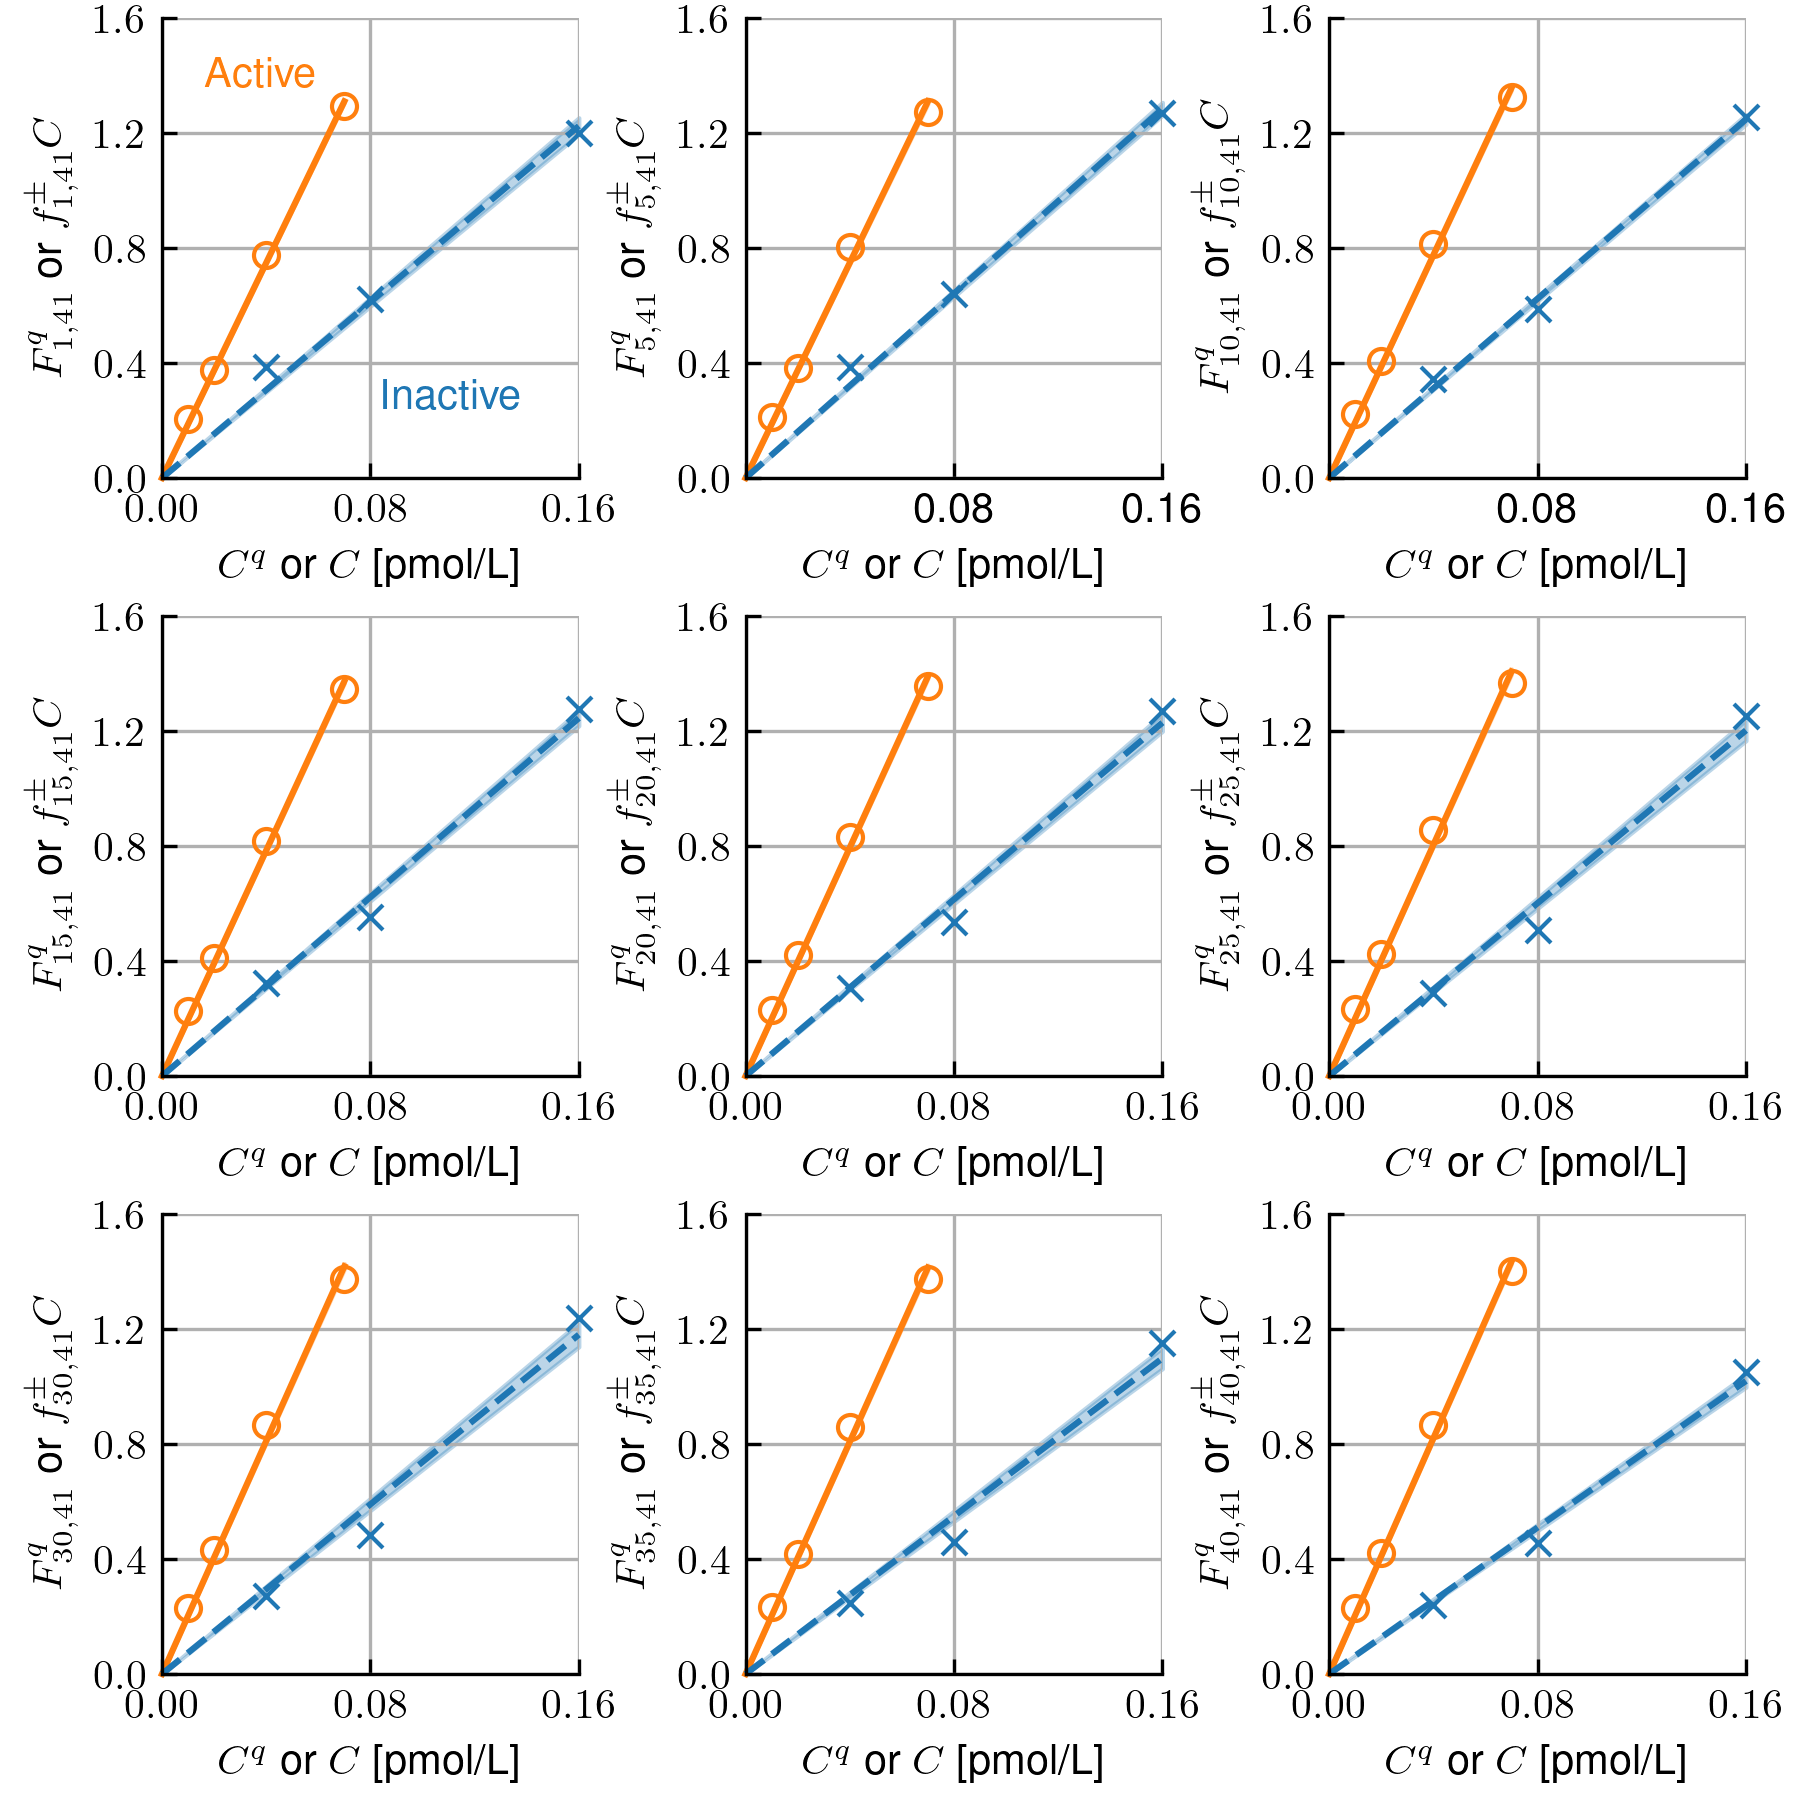
\includegraphics{si-figs/FigS41.png}
                    \caption{
                        As Figure~\ref{fig:S1} with well $w=41$ (or D5).
                    }
                \end{figure}
                \clearpage
    \begin{table}
        \caption{Molar Fluorescence Parameters for Well D5 ($w=41$)}
        \centering
        \begin{tabular}{c|ll|ll}
            Cycle & \multicolumn{2}{c|}{Inactive} & \multicolumn{2}{c}{Active} \\
            \hline
            $i$ & $f_{i,41}^{-}$ & $\sigma_{i,41}^{-}$ &  $f_{i,41}^{+}$ & $\sigma_{i,41}^{+}$ \\
            \hline
    1 & 7.65 & 0.060 & 18.71 & 0.020 \\
2 & 7.63 & 0.057 & 18.15 & 0.030 \\
3 & 7.85 & 0.054 & 18.43 & 0.035 \\
4 & 7.93 & 0.053 & 18.59 & 0.039 \\
5 & 8.03 & 0.047 & 18.72 & 0.040 \\
6 & 7.97 & 0.042 & 18.79 & 0.041 \\
7 & 7.93 & 0.038 & 19.02 & 0.037 \\
8 & 7.88 & 0.035 & 19.13 & 0.037 \\
9 & 7.84 & 0.034 & 19.36 & 0.034 \\
10 & 7.80 & 0.035 & 19.39 & 0.035 \\
11 & 7.75 & 0.035 & 19.48 & 0.033 \\
12 & 7.71 & 0.037 & 19.50 & 0.033 \\
13 & 7.76 & 0.043 & 19.56 & 0.033 \\
14 & 7.80 & 0.050 & 19.59 & 0.032 \\
15 & 7.78 & 0.055 & 19.62 & 0.032 \\
16 & 7.79 & 0.054 & 19.67 & 0.031 \\
17 & 7.75 & 0.055 & 19.70 & 0.031 \\
18 & 7.71 & 0.056 & 19.72 & 0.033 \\
19 & 7.72 & 0.061 & 19.77 & 0.032 \\
20 & 7.68 & 0.062 & 19.86 & 0.036 \\
21 & 7.65 & 0.067 & 19.87 & 0.036 \\
22 & 7.63 & 0.069 & 19.94 & 0.039 \\
23 & 7.55 & 0.069 & 20.01 & 0.043 \\
24 & 7.52 & 0.071 & 20.05 & 0.043 \\
25 & 7.51 & 0.075 & 20.10 & 0.043 \\
26 & 7.46 & 0.076 & 20.13 & 0.043 \\
27 & 7.47 & 0.079 & 20.16 & 0.045 \\
28 & 7.45 & 0.082 & 20.30 & 0.041 \\
29 & 7.42 & 0.085 & 20.24 & 0.046 \\
30 & 7.38 & 0.088 & 20.26 & 0.047 \\
31 & 7.22 & 0.084 & 20.22 & 0.041 \\
32 & 7.19 & 0.080 & 20.22 & 0.039 \\
33 & 7.16 & 0.085 & 20.24 & 0.039 \\
34 & 7.12 & 0.086 & 20.28 & 0.038 \\
35 & 6.86 & 0.076 & 20.19 & 0.042 \\
36 & 6.81 & 0.077 & 20.26 & 0.040 \\
37 & 6.78 & 0.081 & 20.34 & 0.038 \\
38 & 6.38 & 0.055 & 20.36 & 0.038 \\
39 & 6.36 & 0.055 & 20.44 & 0.036 \\
40 & 6.37 & 0.045 & 20.50 & 0.036 \\
41 & 6.32 & 0.047 & 20.26 & 0.044 \\
42 & 6.36 & 0.060 & 20.32 & 0.044 \\
43 & 6.35 & 0.061 & 20.39 & 0.044 \\
44 & 6.32 & 0.063 & 20.41 & 0.045 \\
45 & 6.30 & 0.065 & 20.36 & 0.044 \\
               \hline
        \end{tabular}
    \end{table}
    \clearpage

                \begin{figure}
                    \centering
                    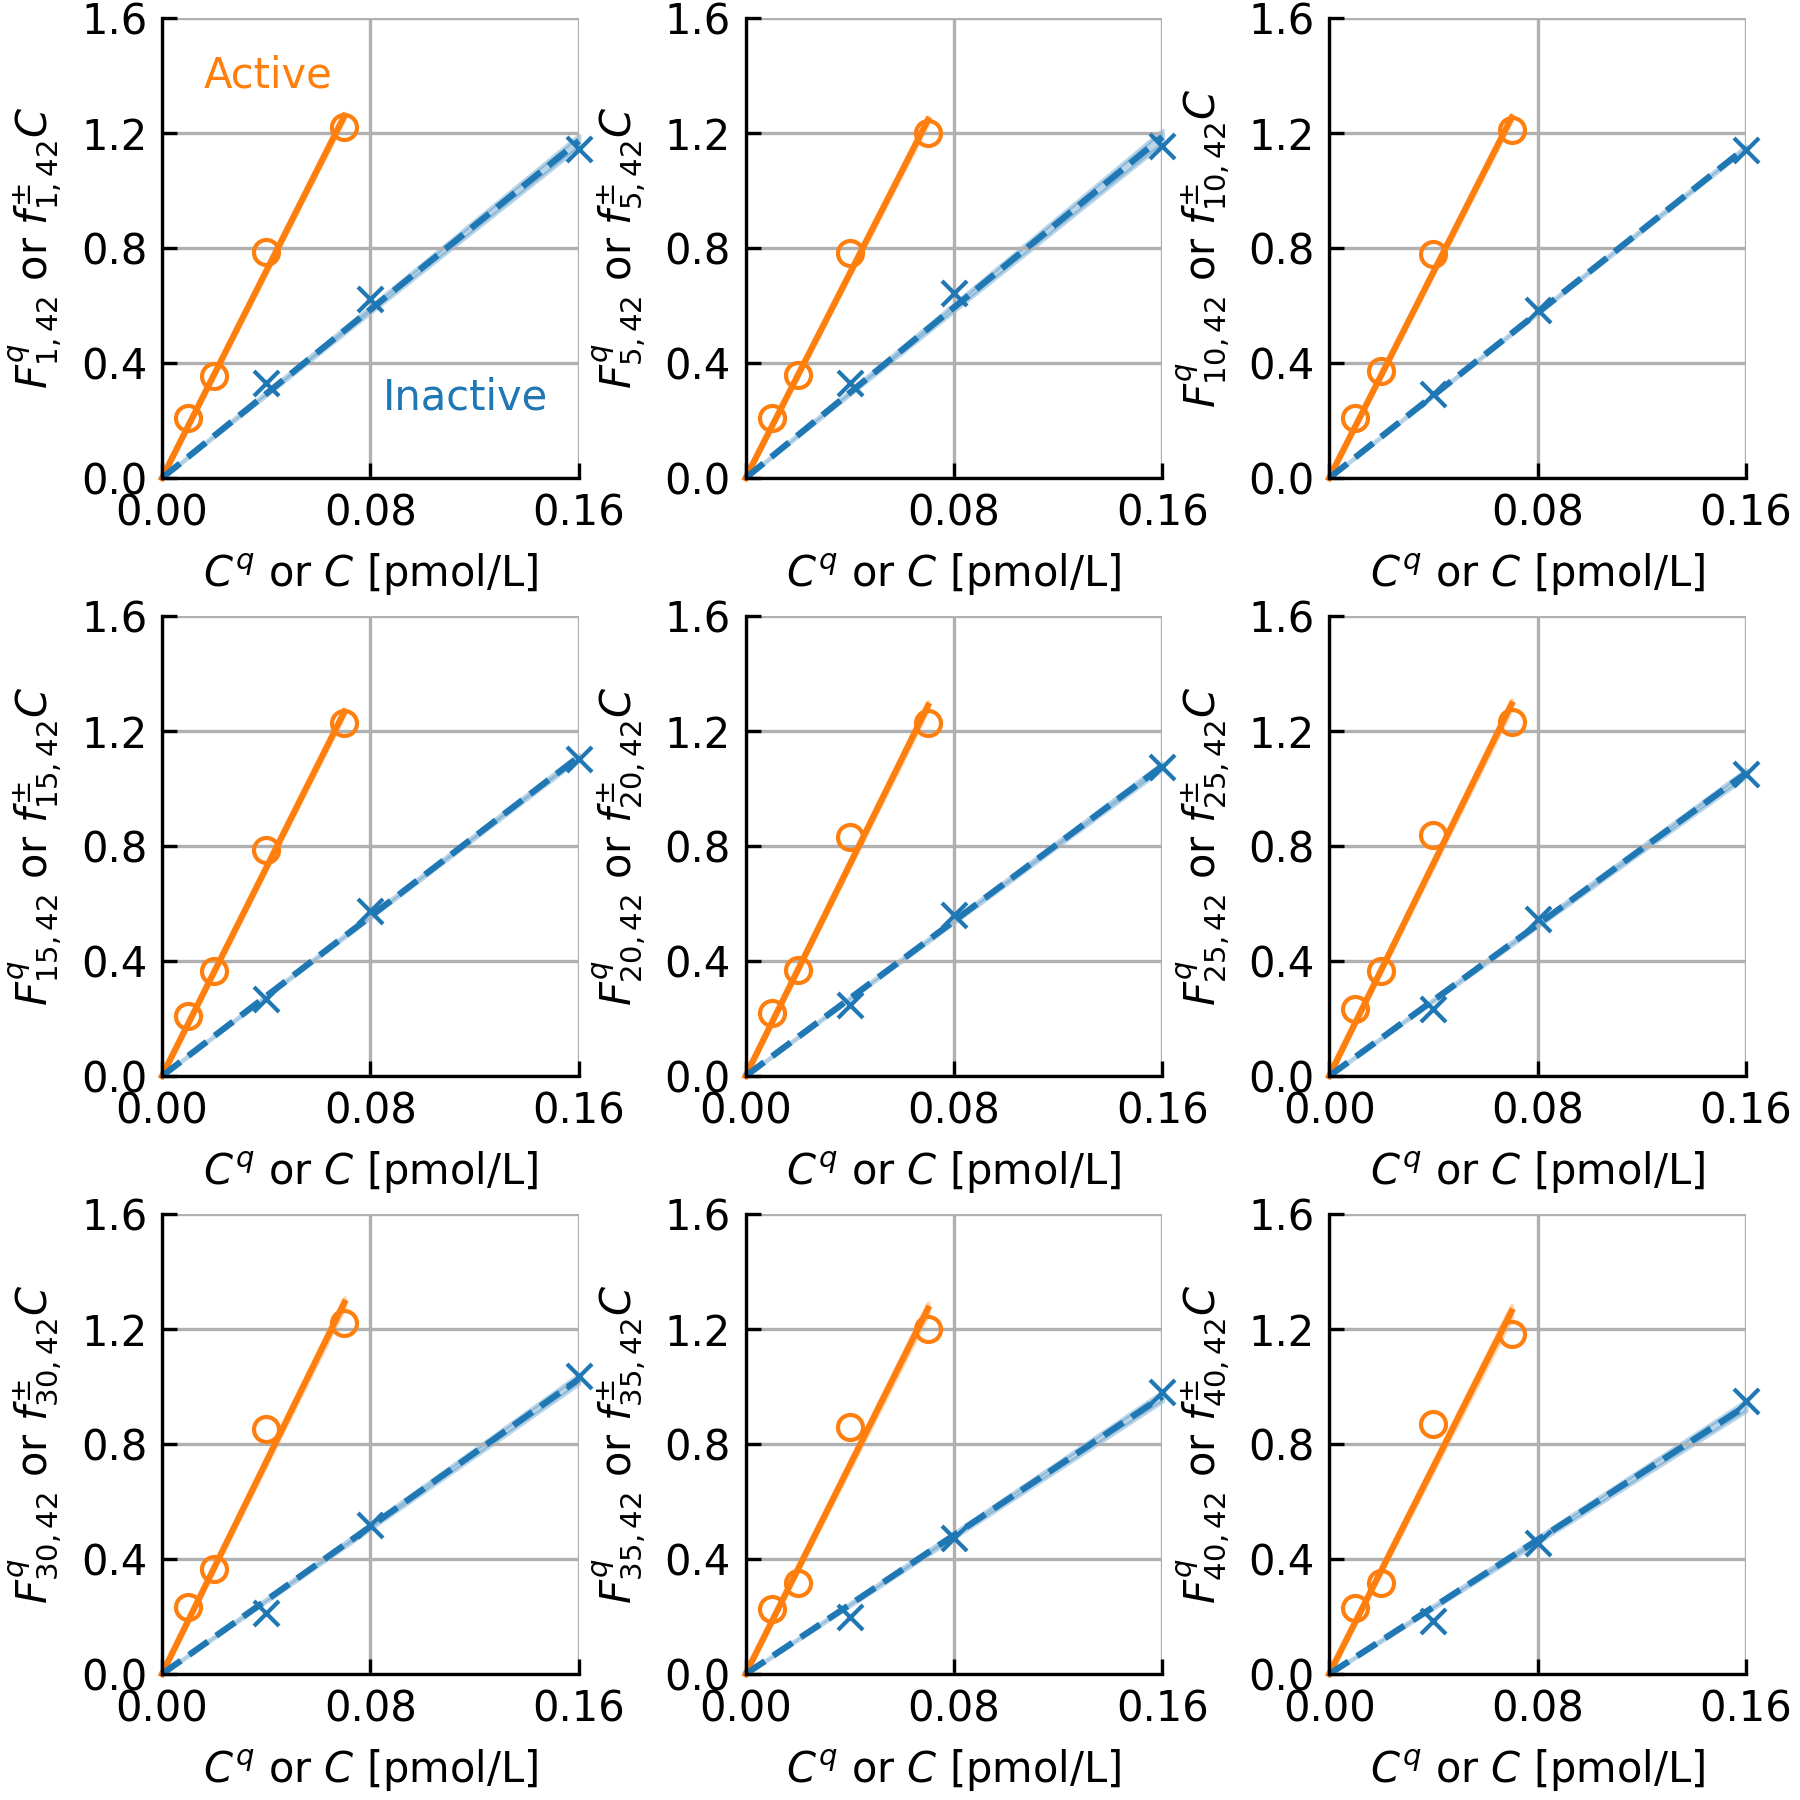
\includegraphics{si-figs/FigS42.png}
                    \caption{
                        As Figure~\ref{fig:S1} with well $w=42$ (or D6).
                    }
                \end{figure}
                \clearpage
    \begin{table}
        \caption{Molar Fluorescence Parameters for Well D6 ($w=42$)}
        \centering
        \begin{tabular}{c|ll|ll}
            Cycle & \multicolumn{2}{c|}{Inactive} & \multicolumn{2}{c}{Active} \\
            \hline
            $i$ & $f_{i,42}^{-}$ & $\sigma_{i,42}^{-}$ &  $f_{i,42}^{+}$ & $\sigma_{i,42}^{+}$ \\
            \hline
    1 & 7.32 & 0.042 & 17.99 & 0.047 \\
2 & 7.15 & 0.049 & 17.39 & 0.048 \\
3 & 7.37 & 0.047 & 17.62 & 0.050 \\
4 & 7.45 & 0.049 & 17.70 & 0.052 \\
5 & 7.41 & 0.048 & 17.79 & 0.051 \\
6 & 7.32 & 0.046 & 17.83 & 0.051 \\
7 & 7.27 & 0.036 & 17.86 & 0.051 \\
8 & 7.24 & 0.025 & 17.89 & 0.050 \\
9 & 7.24 & 0.014 & 17.92 & 0.050 \\
10 & 7.18 & 0.010 & 17.91 & 0.049 \\
11 & 7.14 & 0.013 & 17.94 & 0.048 \\
12 & 7.09 & 0.011 & 17.95 & 0.048 \\
13 & 7.050 & 0.0095 & 17.97 & 0.047 \\
14 & 7.00 & 0.012 & 18.05 & 0.049 \\
15 & 6.94 & 0.017 & 18.10 & 0.046 \\
16 & 6.90 & 0.017 & 18.19 & 0.047 \\
17 & 6.86 & 0.018 & 18.29 & 0.052 \\
18 & 6.81 & 0.019 & 18.42 & 0.061 \\
19 & 6.76 & 0.021 & 18.45 & 0.065 \\
20 & 6.74 & 0.022 & 18.40 & 0.068 \\
21 & 6.71 & 0.024 & 18.39 & 0.068 \\
22 & 6.67 & 0.024 & 18.40 & 0.070 \\
23 & 6.62 & 0.025 & 18.43 & 0.071 \\
24 & 6.62 & 0.024 & 18.47 & 0.073 \\
25 & 6.58 & 0.026 & 18.47 & 0.074 \\
26 & 6.56 & 0.027 & 18.62 & 0.072 \\
27 & 6.51 & 0.026 & 18.52 & 0.076 \\
28 & 6.49 & 0.029 & 18.51 & 0.078 \\
29 & 6.46 & 0.031 & 18.50 & 0.079 \\
30 & 6.41 & 0.033 & 18.45 & 0.082 \\
31 & 6.36 & 0.034 & 18.46 & 0.082 \\
32 & 6.33 & 0.035 & 18.48 & 0.084 \\
33 & 6.16 & 0.032 & 18.38 & 0.085 \\
34 & 6.12 & 0.033 & 18.35 & 0.087 \\
35 & 6.03 & 0.034 & 18.15 & 0.094 \\
36 & 6.01 & 0.036 & 18.11 & 0.097 \\
37 & 5.99 & 0.037 & 18.06 & 0.099 \\
38 & 5.96 & 0.038 & 18.12 & 0.099 \\
39 & 5.71 & 0.028 & 18.0 & 0.10 \\
40 & 5.83 & 0.037 & 18.0 & 0.11 \\
41 & 5.80 & 0.037 & 17.9 & 0.10 \\
42 & 5.78 & 0.038 & 17.9 & 0.10 \\
43 & 5.76 & 0.040 & 17.9 & 0.11 \\
44 & 5.77 & 0.040 & 17.0 & 0.13 \\
45 & 5.74 & 0.043 & 16.9 & 0.13 \\
               \hline
        \end{tabular}
    \end{table}
    \clearpage

                \begin{figure}
                    \centering
                    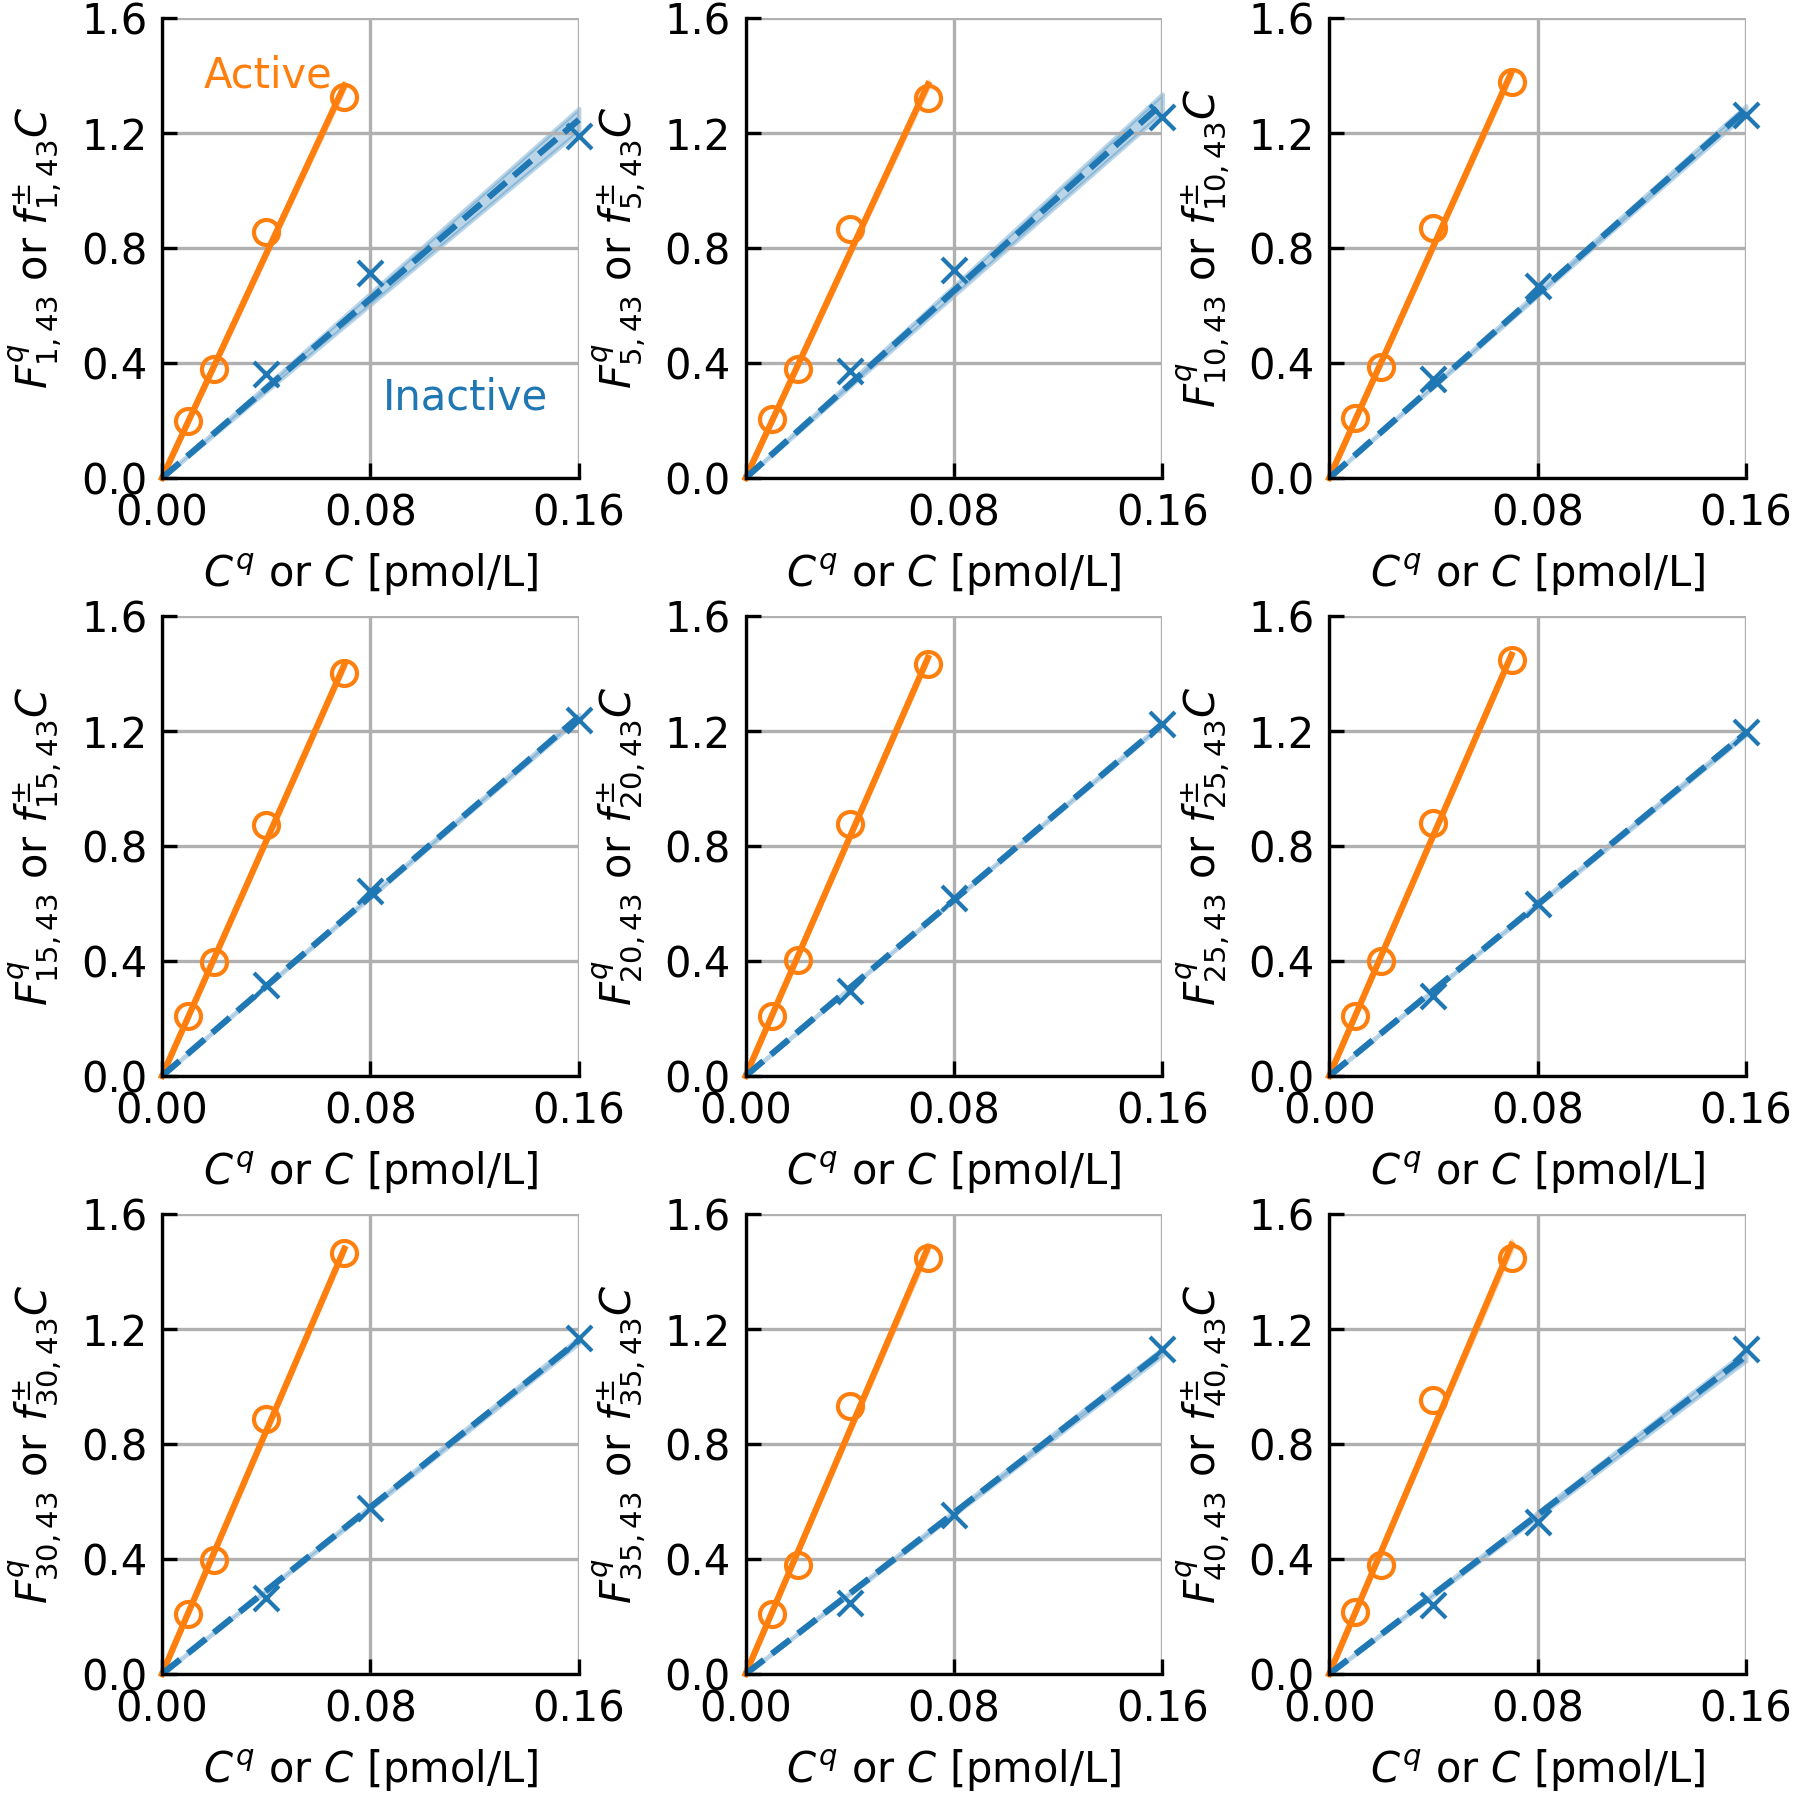
\includegraphics{si-figs/FigS43.png}
                    \caption{
                        As Figure~\ref{fig:S1} with well $w=43$ (or D7).
                    }
                \end{figure}
                \clearpage
    \begin{table}
        \caption{Molar Fluorescence Parameters for Well D7 ($w=43$)}
        \centering
        \begin{tabular}{c|ll|ll}
            Cycle & \multicolumn{2}{c|}{Inactive} & \multicolumn{2}{c}{Active} \\
            \hline
            $i$ & $f_{i,43}^{-}$ & $\sigma_{i,43}^{-}$ &  $f_{i,43}^{+}$ & $\sigma_{i,43}^{+}$ \\
            \hline
    1 & 7.79 & 0.082 & 19.50 & 0.049 \\
2 & 7.82 & 0.075 & 19.02 & 0.054 \\
3 & 8.01 & 0.074 & 19.27 & 0.056 \\
4 & 8.13 & 0.071 & 19.46 & 0.056 \\
5 & 8.14 & 0.069 & 19.56 & 0.056 \\
6 & 8.10 & 0.062 & 19.86 & 0.050 \\
7 & 8.13 & 0.048 & 19.92 & 0.049 \\
8 & 8.08 & 0.040 & 20.00 & 0.047 \\
9 & 8.06 & 0.034 & 20.08 & 0.045 \\
10 & 8.01 & 0.029 & 20.16 & 0.043 \\
11 & 7.99 & 0.027 & 20.18 & 0.043 \\
12 & 7.95 & 0.023 & 20.28 & 0.042 \\
13 & 7.91 & 0.020 & 20.32 & 0.041 \\
14 & 7.86 & 0.017 & 20.36 & 0.040 \\
15 & 7.81 & 0.015 & 20.44 & 0.037 \\
16 & 7.80 & 0.013 & 20.49 & 0.037 \\
17 & 7.743 & 0.0098 & 20.55 & 0.033 \\
18 & 7.698 & 0.0083 & 20.64 & 0.034 \\
19 & 7.650 & 0.0091 & 20.73 & 0.032 \\
20 & 7.656 & 0.0080 & 20.78 & 0.031 \\
21 & 7.562 & 0.0082 & 20.88 & 0.029 \\
22 & 7.519 & 0.0085 & 20.90 & 0.031 \\
23 & 7.482 & 0.0089 & 20.86 & 0.030 \\
24 & 7.48 & 0.010 & 20.90 & 0.029 \\
25 & 7.46 & 0.014 & 20.93 & 0.029 \\
26 & 7.43 & 0.013 & 20.99 & 0.030 \\
27 & 7.38 & 0.015 & 21.03 & 0.029 \\
28 & 7.36 & 0.017 & 21.08 & 0.028 \\
29 & 7.33 & 0.020 & 21.13 & 0.029 \\
30 & 7.25 & 0.020 & 21.13 & 0.029 \\
31 & 7.24 & 0.022 & 20.86 & 0.035 \\
32 & 7.07 & 0.018 & 20.92 & 0.035 \\
33 & 7.06 & 0.019 & 20.95 & 0.034 \\
34 & 7.03 & 0.025 & 21.13 & 0.049 \\
35 & 7.00 & 0.025 & 21.19 & 0.059 \\
36 & 7.00 & 0.027 & 21.09 & 0.063 \\
37 & 6.97 & 0.031 & 21.16 & 0.061 \\
38 & 6.95 & 0.034 & 21.23 & 0.064 \\
39 & 6.93 & 0.035 & 21.30 & 0.066 \\
40 & 6.92 & 0.036 & 21.33 & 0.069 \\
41 & 6.93 & 0.040 & 21.39 & 0.069 \\
42 & 6.91 & 0.042 & 21.36 & 0.072 \\
43 & 6.81 & 0.037 & 21.50 & 0.071 \\
44 & 6.39 & 0.020 & 21.51 & 0.073 \\
45 & 6.38 & 0.020 & 20.79 & 0.079 \\
               \hline
        \end{tabular}
    \end{table}
    \clearpage

                \begin{figure}
                    \centering
                    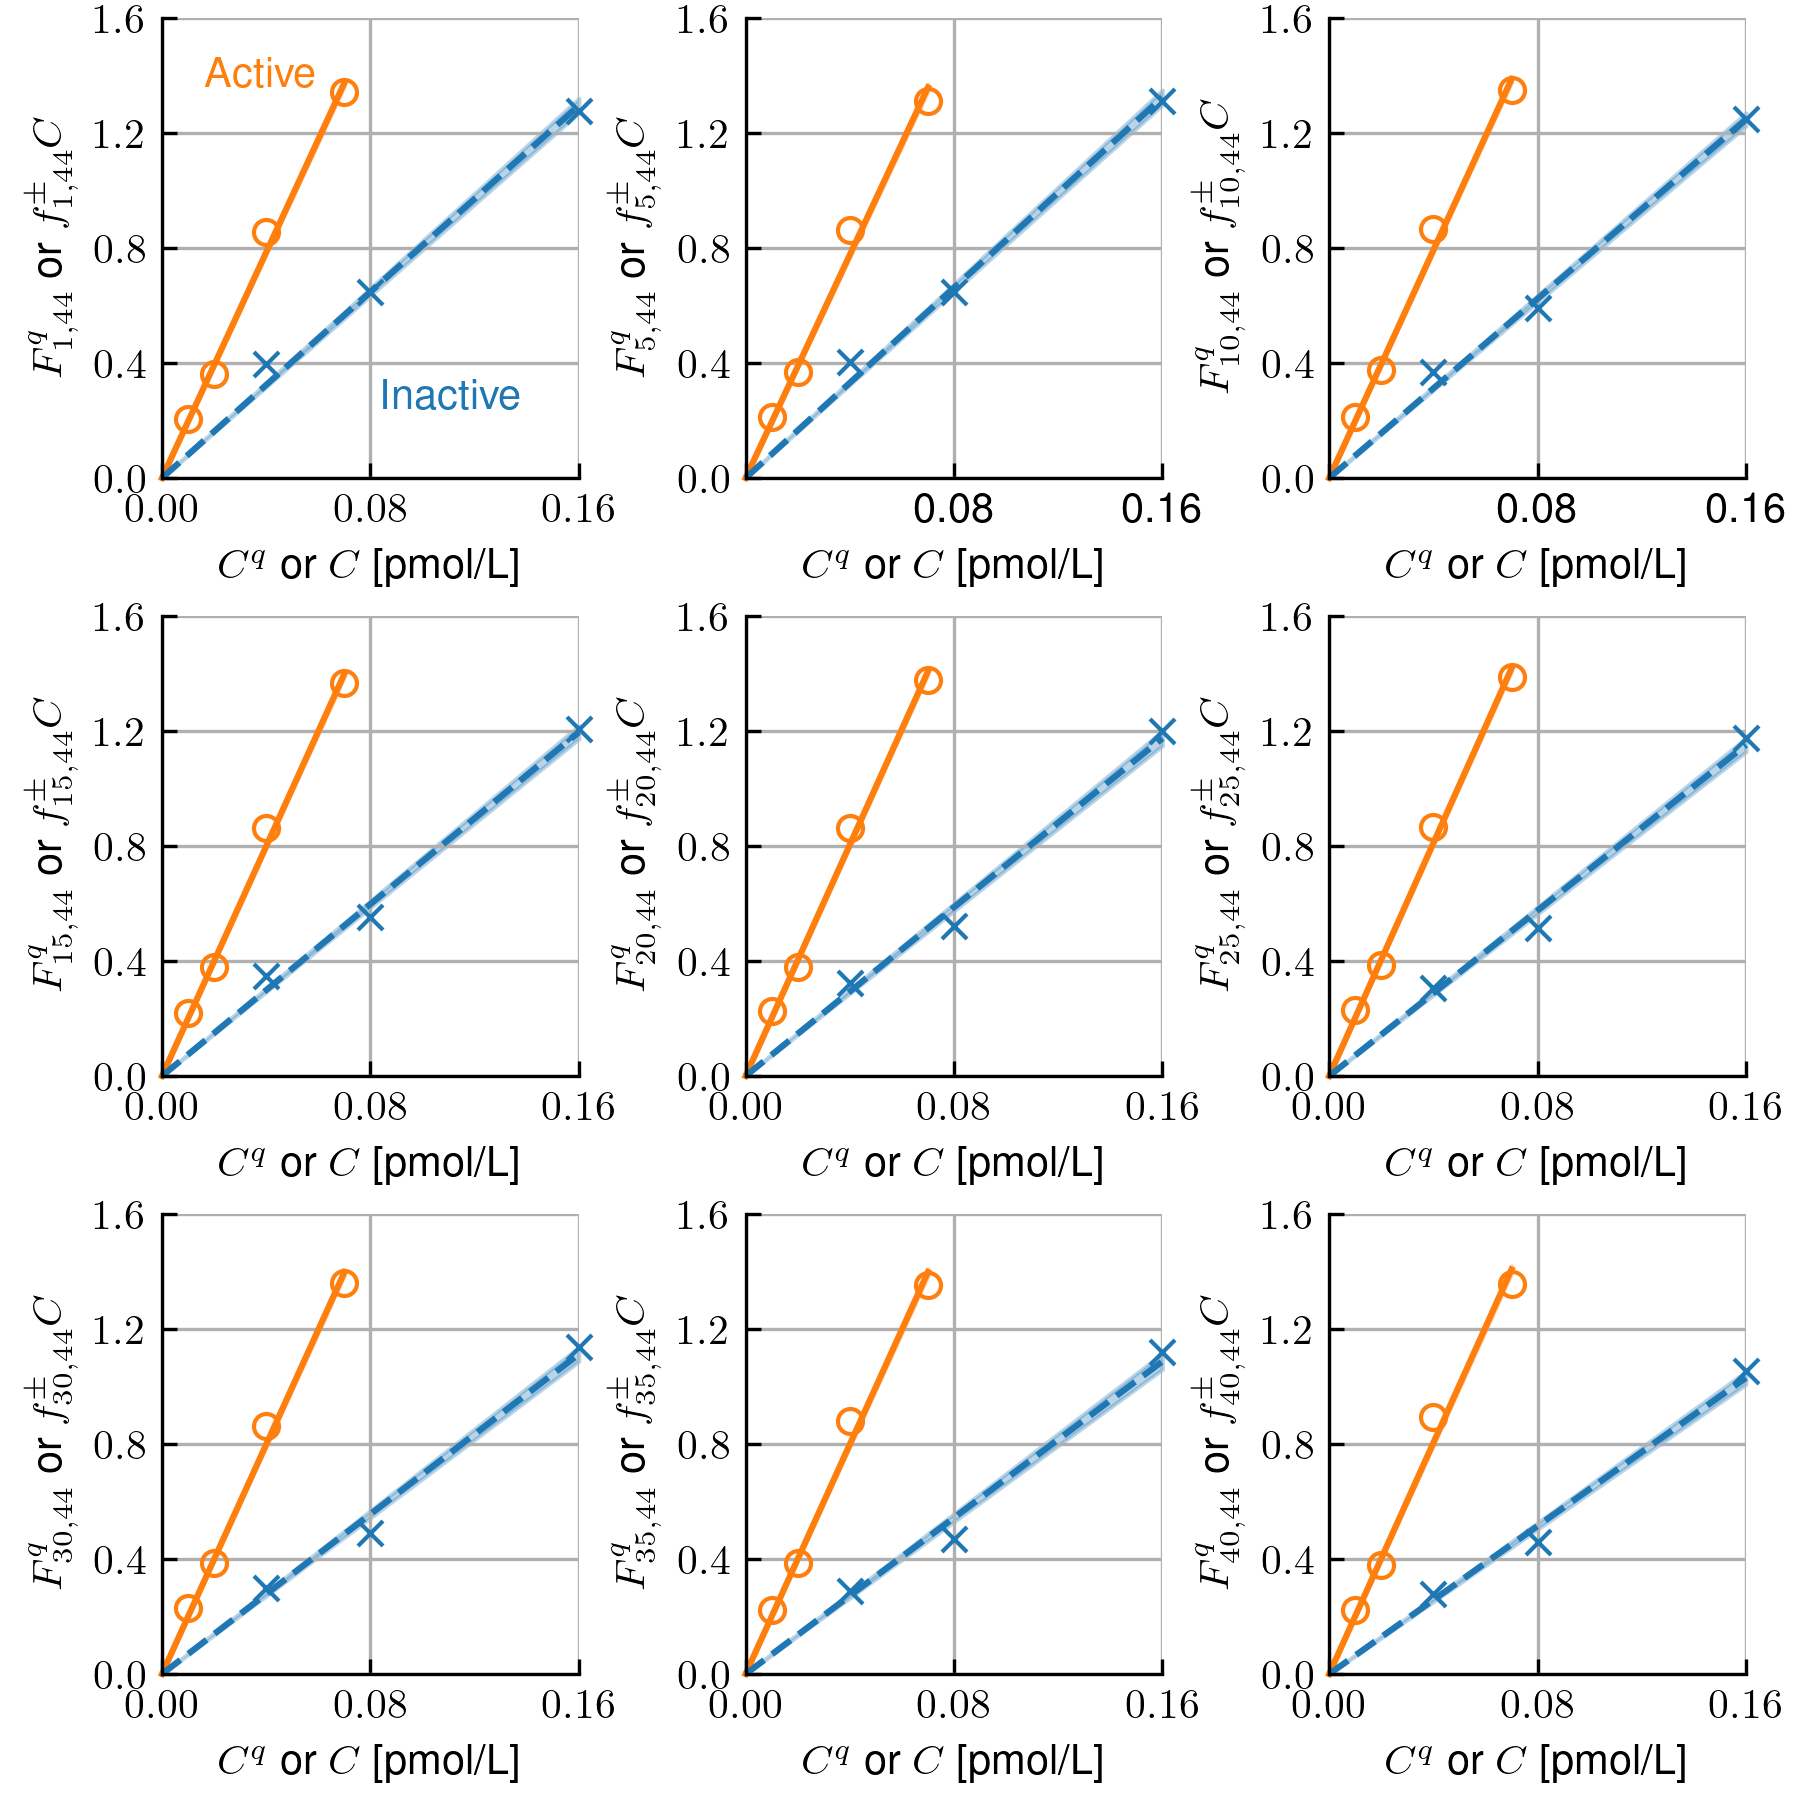
\includegraphics{si-figs/FigS44.png}
                    \caption{
                        As Figure~\ref{fig:S1} with well $w=44$ (or D8).
                    }
                \end{figure}
                \clearpage
    \begin{table}
        \caption{Molar Fluorescence Parameters for Well D8 ($w=44$)}
        \centering
        \begin{tabular}{c|ll|ll}
            Cycle & \multicolumn{2}{c|}{Inactive} & \multicolumn{2}{c}{Active} \\
            \hline
            $i$ & $f_{i,44}^{-}$ & $\sigma_{i,44}^{-}$ &  $f_{i,44}^{+}$ & $\sigma_{i,44}^{+}$ \\
            \hline
    1 & 8.09 & 0.052 & 19.63 & 0.048 \\
2 & 8.04 & 0.055 & 18.98 & 0.056 \\
3 & 8.21 & 0.054 & 19.15 & 0.058 \\
4 & 8.30 & 0.053 & 19.33 & 0.059 \\
5 & 8.27 & 0.053 & 19.40 & 0.058 \\
6 & 8.20 & 0.050 & 19.46 & 0.057 \\
7 & 8.13 & 0.049 & 19.65 & 0.053 \\
8 & 8.02 & 0.048 & 19.71 & 0.052 \\
9 & 7.89 & 0.048 & 19.77 & 0.049 \\
10 & 7.79 & 0.047 & 19.81 & 0.049 \\
11 & 7.70 & 0.047 & 19.88 & 0.048 \\
12 & 7.61 & 0.046 & 19.92 & 0.047 \\
13 & 7.54 & 0.045 & 19.92 & 0.046 \\
14 & 7.52 & 0.047 & 19.93 & 0.046 \\
15 & 7.47 & 0.048 & 19.98 & 0.045 \\
16 & 7.45 & 0.049 & 20.03 & 0.044 \\
17 & 7.38 & 0.048 & 20.05 & 0.044 \\
18 & 7.36 & 0.051 & 20.10 & 0.046 \\
19 & 7.36 & 0.052 & 20.11 & 0.043 \\
20 & 7.34 & 0.053 & 20.11 & 0.043 \\
21 & 7.30 & 0.053 & 20.15 & 0.042 \\
22 & 7.27 & 0.051 & 20.17 & 0.042 \\
23 & 7.28 & 0.051 & 20.19 & 0.041 \\
24 & 7.23 & 0.048 & 20.27 & 0.045 \\
25 & 7.20 & 0.049 & 20.25 & 0.042 \\
26 & 7.17 & 0.051 & 20.26 & 0.040 \\
27 & 7.13 & 0.051 & 20.23 & 0.042 \\
28 & 7.03 & 0.047 & 20.15 & 0.043 \\
29 & 6.98 & 0.049 & 20.06 & 0.045 \\
30 & 6.95 & 0.051 & 19.96 & 0.047 \\
31 & 6.91 & 0.052 & 19.96 & 0.045 \\
32 & 6.87 & 0.053 & 19.69 & 0.052 \\
33 & 6.84 & 0.054 & 19.92 & 0.048 \\
34 & 6.81 & 0.054 & 19.86 & 0.047 \\
35 & 6.80 & 0.057 & 19.97 & 0.056 \\
36 & 6.74 & 0.052 & 19.97 & 0.059 \\
37 & 6.71 & 0.055 & 20.01 & 0.060 \\
38 & 6.54 & 0.047 & 20.02 & 0.061 \\
39 & 6.47 & 0.046 & 20.04 & 0.062 \\
40 & 6.44 & 0.046 & 20.10 & 0.062 \\
41 & 6.40 & 0.046 & 19.83 & 0.066 \\
42 & 6.34 & 0.045 & 19.82 & 0.067 \\
43 & 6.29 & 0.046 & 19.79 & 0.067 \\
44 & 6.25 & 0.049 & 19.70 & 0.071 \\
45 & 6.23 & 0.047 & 18.83 & 0.094 \\
               \hline
        \end{tabular}
    \end{table}
    \clearpage

                \begin{figure}
                    \centering
                    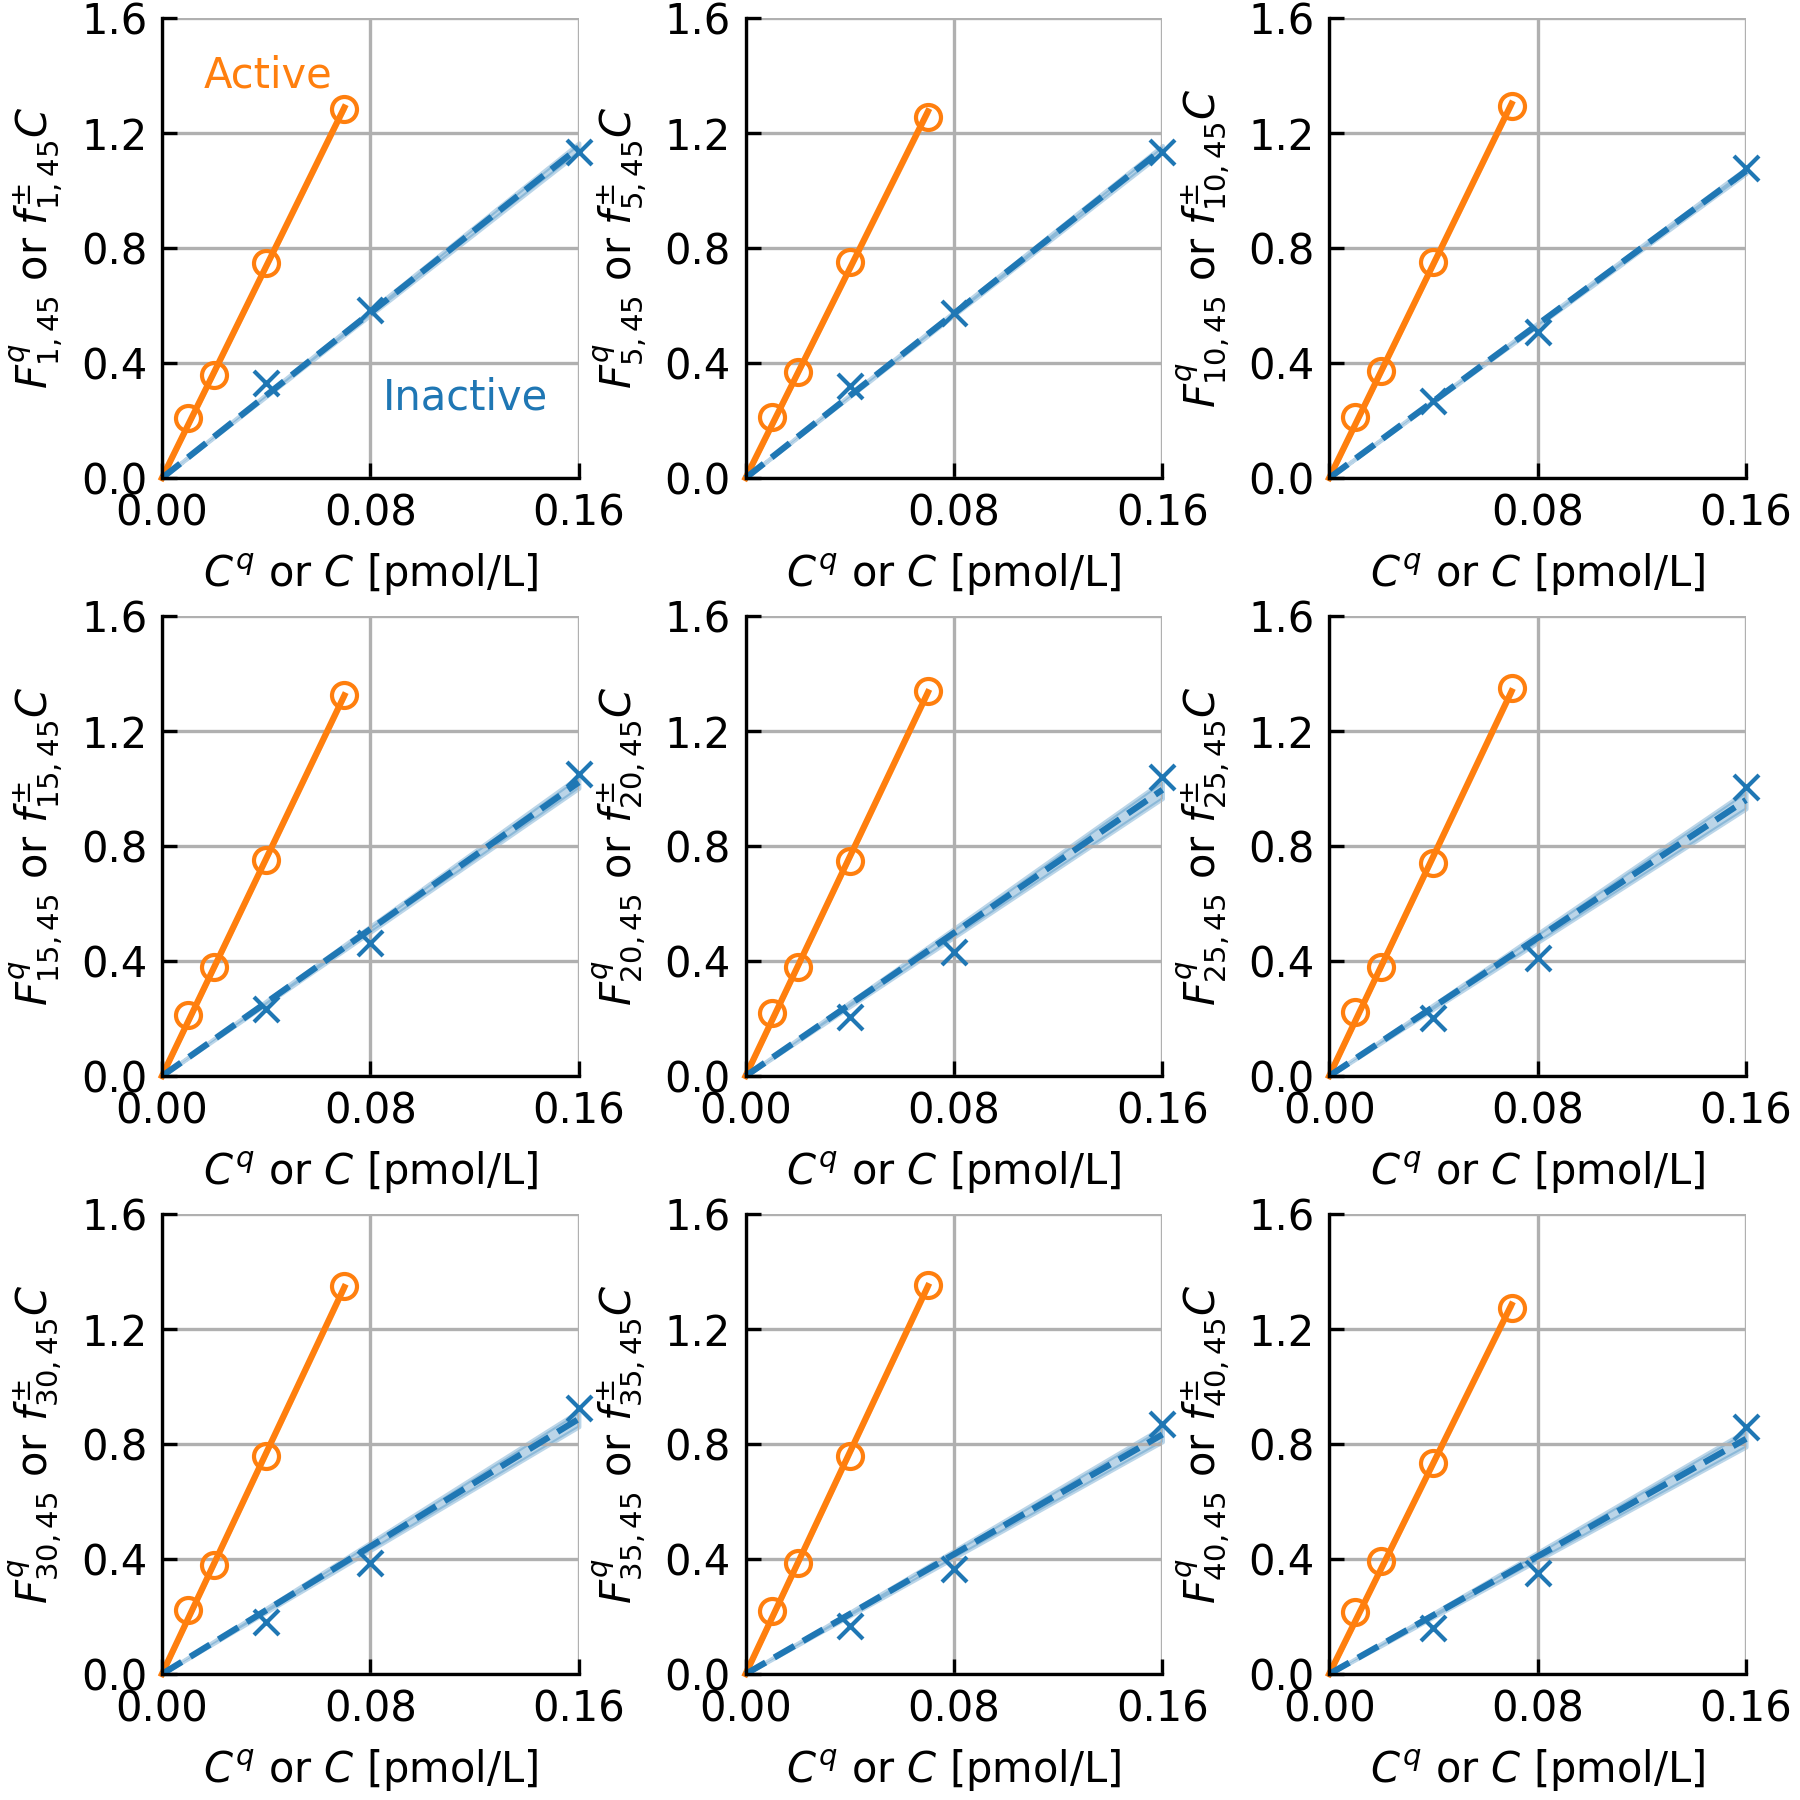
\includegraphics{si-figs/FigS45.png}
                    \caption{
                        As Figure~\ref{fig:S1} with well $w=45$ (or D9).
                    }
                \end{figure}
                \clearpage
    \begin{table}
        \caption{Molar Fluorescence Parameters for Well D9 ($w=45$)}
        \centering
        \begin{tabular}{c|ll|ll}
            Cycle & \multicolumn{2}{c|}{Inactive} & \multicolumn{2}{c}{Active} \\
            \hline
            $i$ & $f_{i,45}^{-}$ & $\sigma_{i,45}^{-}$ &  $f_{i,45}^{+}$ & $\sigma_{i,45}^{+}$ \\
            \hline
    1 & 7.18 & 0.033 & 18.41 & 0.018 \\
2 & 7.22 & 0.044 & 17.80 & 0.021 \\
3 & 7.36 & 0.036 & 18.02 & 0.025 \\
4 & 7.27 & 0.031 & 18.14 & 0.025 \\
5 & 7.15 & 0.026 & 18.22 & 0.025 \\
6 & 7.05 & 0.020 & 18.35 & 0.022 \\
7 & 6.95 & 0.016 & 18.41 & 0.021 \\
8 & 6.87 & 0.015 & 18.48 & 0.020 \\
9 & 6.76 & 0.017 & 18.57 & 0.018 \\
10 & 6.67 & 0.019 & 18.60 & 0.018 \\
11 & 6.60 & 0.024 & 18.67 & 0.016 \\
12 & 6.54 & 0.029 & 18.70 & 0.016 \\
13 & 6.51 & 0.034 & 18.79 & 0.015 \\
14 & 6.42 & 0.039 & 18.86 & 0.015 \\
15 & 6.38 & 0.043 & 18.91 & 0.015 \\
16 & 6.30 & 0.044 & 18.97 & 0.015 \\
17 & 6.39 & 0.058 & 18.99 & 0.015 \\
18 & 6.33 & 0.060 & 19.02 & 0.015 \\
19 & 6.27 & 0.062 & 19.07 & 0.018 \\
20 & 6.22 & 0.063 & 19.07 & 0.019 \\
21 & 6.17 & 0.061 & 19.06 & 0.021 \\
22 & 6.11 & 0.061 & 19.09 & 0.021 \\
23 & 6.04 & 0.059 & 19.11 & 0.024 \\
24 & 5.98 & 0.060 & 19.14 & 0.025 \\
25 & 6.00 & 0.064 & 19.12 & 0.023 \\
26 & 5.95 & 0.069 & 19.12 & 0.022 \\
27 & 5.90 & 0.067 & 19.20 & 0.020 \\
28 & 5.68 & 0.059 & 19.25 & 0.019 \\
29 & 5.59 & 0.058 & 19.21 & 0.019 \\
30 & 5.55 & 0.057 & 19.22 & 0.019 \\
31 & 5.33 & 0.046 & 19.13 & 0.019 \\
32 & 5.30 & 0.047 & 19.21 & 0.019 \\
33 & 5.27 & 0.049 & 19.24 & 0.016 \\
34 & 5.24 & 0.052 & 19.27 & 0.017 \\
35 & 5.21 & 0.052 & 19.27 & 0.018 \\
36 & 5.17 & 0.057 & 18.41 & 0.029 \\
37 & 5.15 & 0.059 & 18.43 & 0.029 \\
38 & 5.14 & 0.055 & 18.48 & 0.028 \\
39 & 5.13 & 0.056 & 18.50 & 0.028 \\
40 & 5.11 & 0.058 & 18.35 & 0.024 \\
41 & 5.09 & 0.059 & 18.39 & 0.025 \\
42 & 5.08 & 0.061 & 18.40 & 0.022 \\
43 & 5.06 & 0.062 & 18.44 & 0.023 \\
44 & 5.05 & 0.063 & 17.87 & 0.034 \\
45 & 5.03 & 0.063 & 18.06 & 0.031 \\
               \hline
        \end{tabular}
    \end{table}
    \clearpage

                \begin{figure}
                    \centering
                    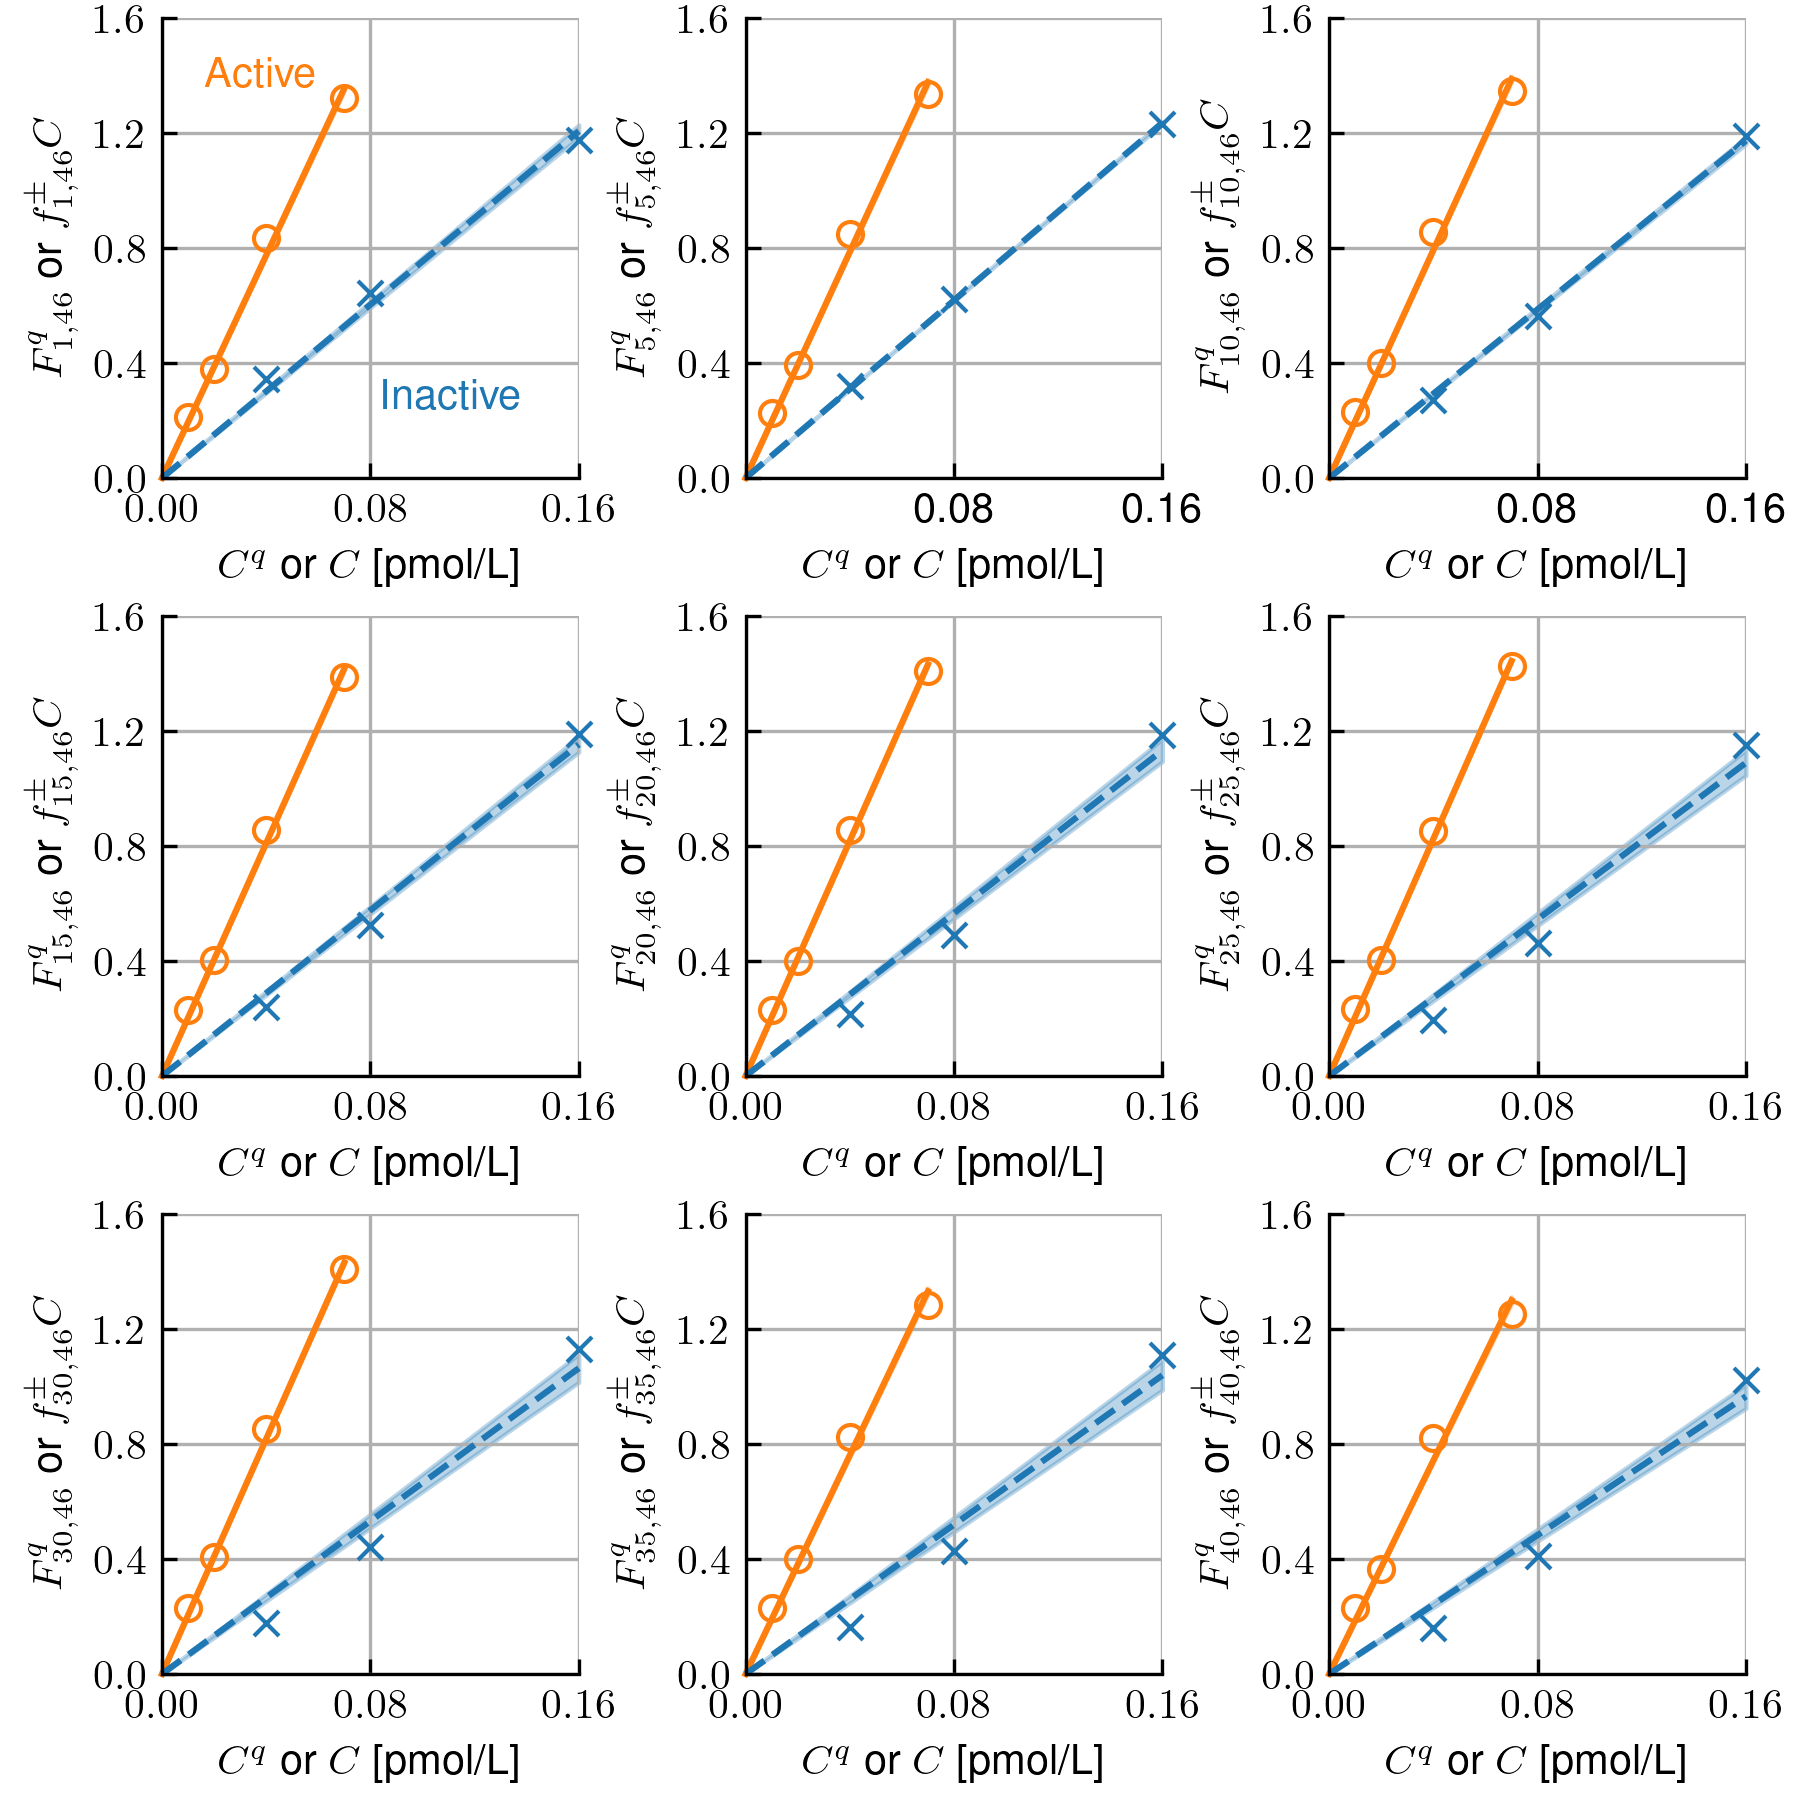
\includegraphics{si-figs/FigS46.png}
                    \caption{
                        As Figure~\ref{fig:S1} with well $w=46$ (or D10).
                    }
                \end{figure}
                \clearpage
    \begin{table}
        \caption{Molar Fluorescence Parameters for Well D10 ($w=46$)}
        \centering
        \begin{tabular}{c|ll|ll}
            Cycle & \multicolumn{2}{c|}{Inactive} & \multicolumn{2}{c}{Active} \\
            \hline
            $i$ & $f_{i,46}^{-}$ & $\sigma_{i,46}^{-}$ &  $f_{i,46}^{+}$ & $\sigma_{i,46}^{+}$ \\
            \hline
    1 & 7.54 & 0.046 & 19.37 & 0.041 \\
2 & 7.67 & 0.037 & 19.14 & 0.044 \\
3 & 7.83 & 0.023 & 19.46 & 0.046 \\
4 & 7.79 & 0.018 & 19.60 & 0.047 \\
5 & 7.725 & 0.0095 & 19.66 & 0.047 \\
6 & 7.628 & 0.0031 & 19.62 & 0.050 \\
7 & 7.563 & 0.0078 & 19.67 & 0.049 \\
8 & 7.49 & 0.014 & 19.75 & 0.048 \\
9 & 7.41 & 0.020 & 19.81 & 0.048 \\
10 & 7.33 & 0.025 & 19.83 & 0.048 \\
11 & 7.25 & 0.028 & 19.86 & 0.047 \\
12 & 7.20 & 0.032 & 19.93 & 0.046 \\
13 & 7.13 & 0.036 & 19.77 & 0.050 \\
14 & 7.07 & 0.040 & 19.87 & 0.047 \\
15 & 7.21 & 0.056 & 20.25 & 0.034 \\
16 & 7.09 & 0.056 & 20.36 & 0.032 \\
17 & 7.18 & 0.069 & 20.43 & 0.031 \\
18 & 7.18 & 0.076 & 20.52 & 0.031 \\
19 & 7.14 & 0.078 & 20.53 & 0.026 \\
20 & 7.08 & 0.081 & 20.45 & 0.030 \\
21 & 6.88 & 0.071 & 20.52 & 0.028 \\
22 & 6.90 & 0.078 & 20.56 & 0.027 \\
23 & 6.84 & 0.080 & 20.59 & 0.025 \\
24 & 6.84 & 0.090 & 20.60 & 0.026 \\
25 & 6.81 & 0.092 & 20.62 & 0.025 \\
26 & 6.78 & 0.092 & 20.63 & 0.022 \\
27 & 6.74 & 0.096 & 20.68 & 0.021 \\
28 & 6.71 & 0.098 & 20.68 & 0.021 \\
29 & 6.67 & 0.099 & 20.65 & 0.021 \\
30 & 6.6 & 0.10 & 20.45 & 0.027 \\
31 & 6.7 & 0.10 & 20.47 & 0.027 \\
32 & 6.6 & 0.10 & 20.47 & 0.026 \\
33 & 6.5 & 0.10 & 20.55 & 0.026 \\
34 & 6.5 & 0.11 & 19.07 & 0.049 \\
35 & 6.5 & 0.11 & 19.02 & 0.052 \\
36 & 6.5 & 0.11 & 18.98 & 0.054 \\
37 & 6.4 & 0.11 & 18.92 & 0.057 \\
38 & 6.4 & 0.11 & 18.73 & 0.057 \\
39 & 6.4 & 0.11 & 18.63 & 0.059 \\
40 & 6.04 & 0.087 & 18.57 & 0.060 \\
41 & 6.02 & 0.088 & 18.49 & 0.062 \\
42 & 5.96 & 0.088 & 18.41 & 0.064 \\
43 & 5.90 & 0.087 & 18.30 & 0.059 \\
44 & 5.35 & 0.054 & 18.09 & 0.064 \\
45 & 5.34 & 0.055 & 18.06 & 0.069 \\
               \hline
        \end{tabular}
    \end{table}
    \clearpage

                \begin{figure}
                    \centering
                    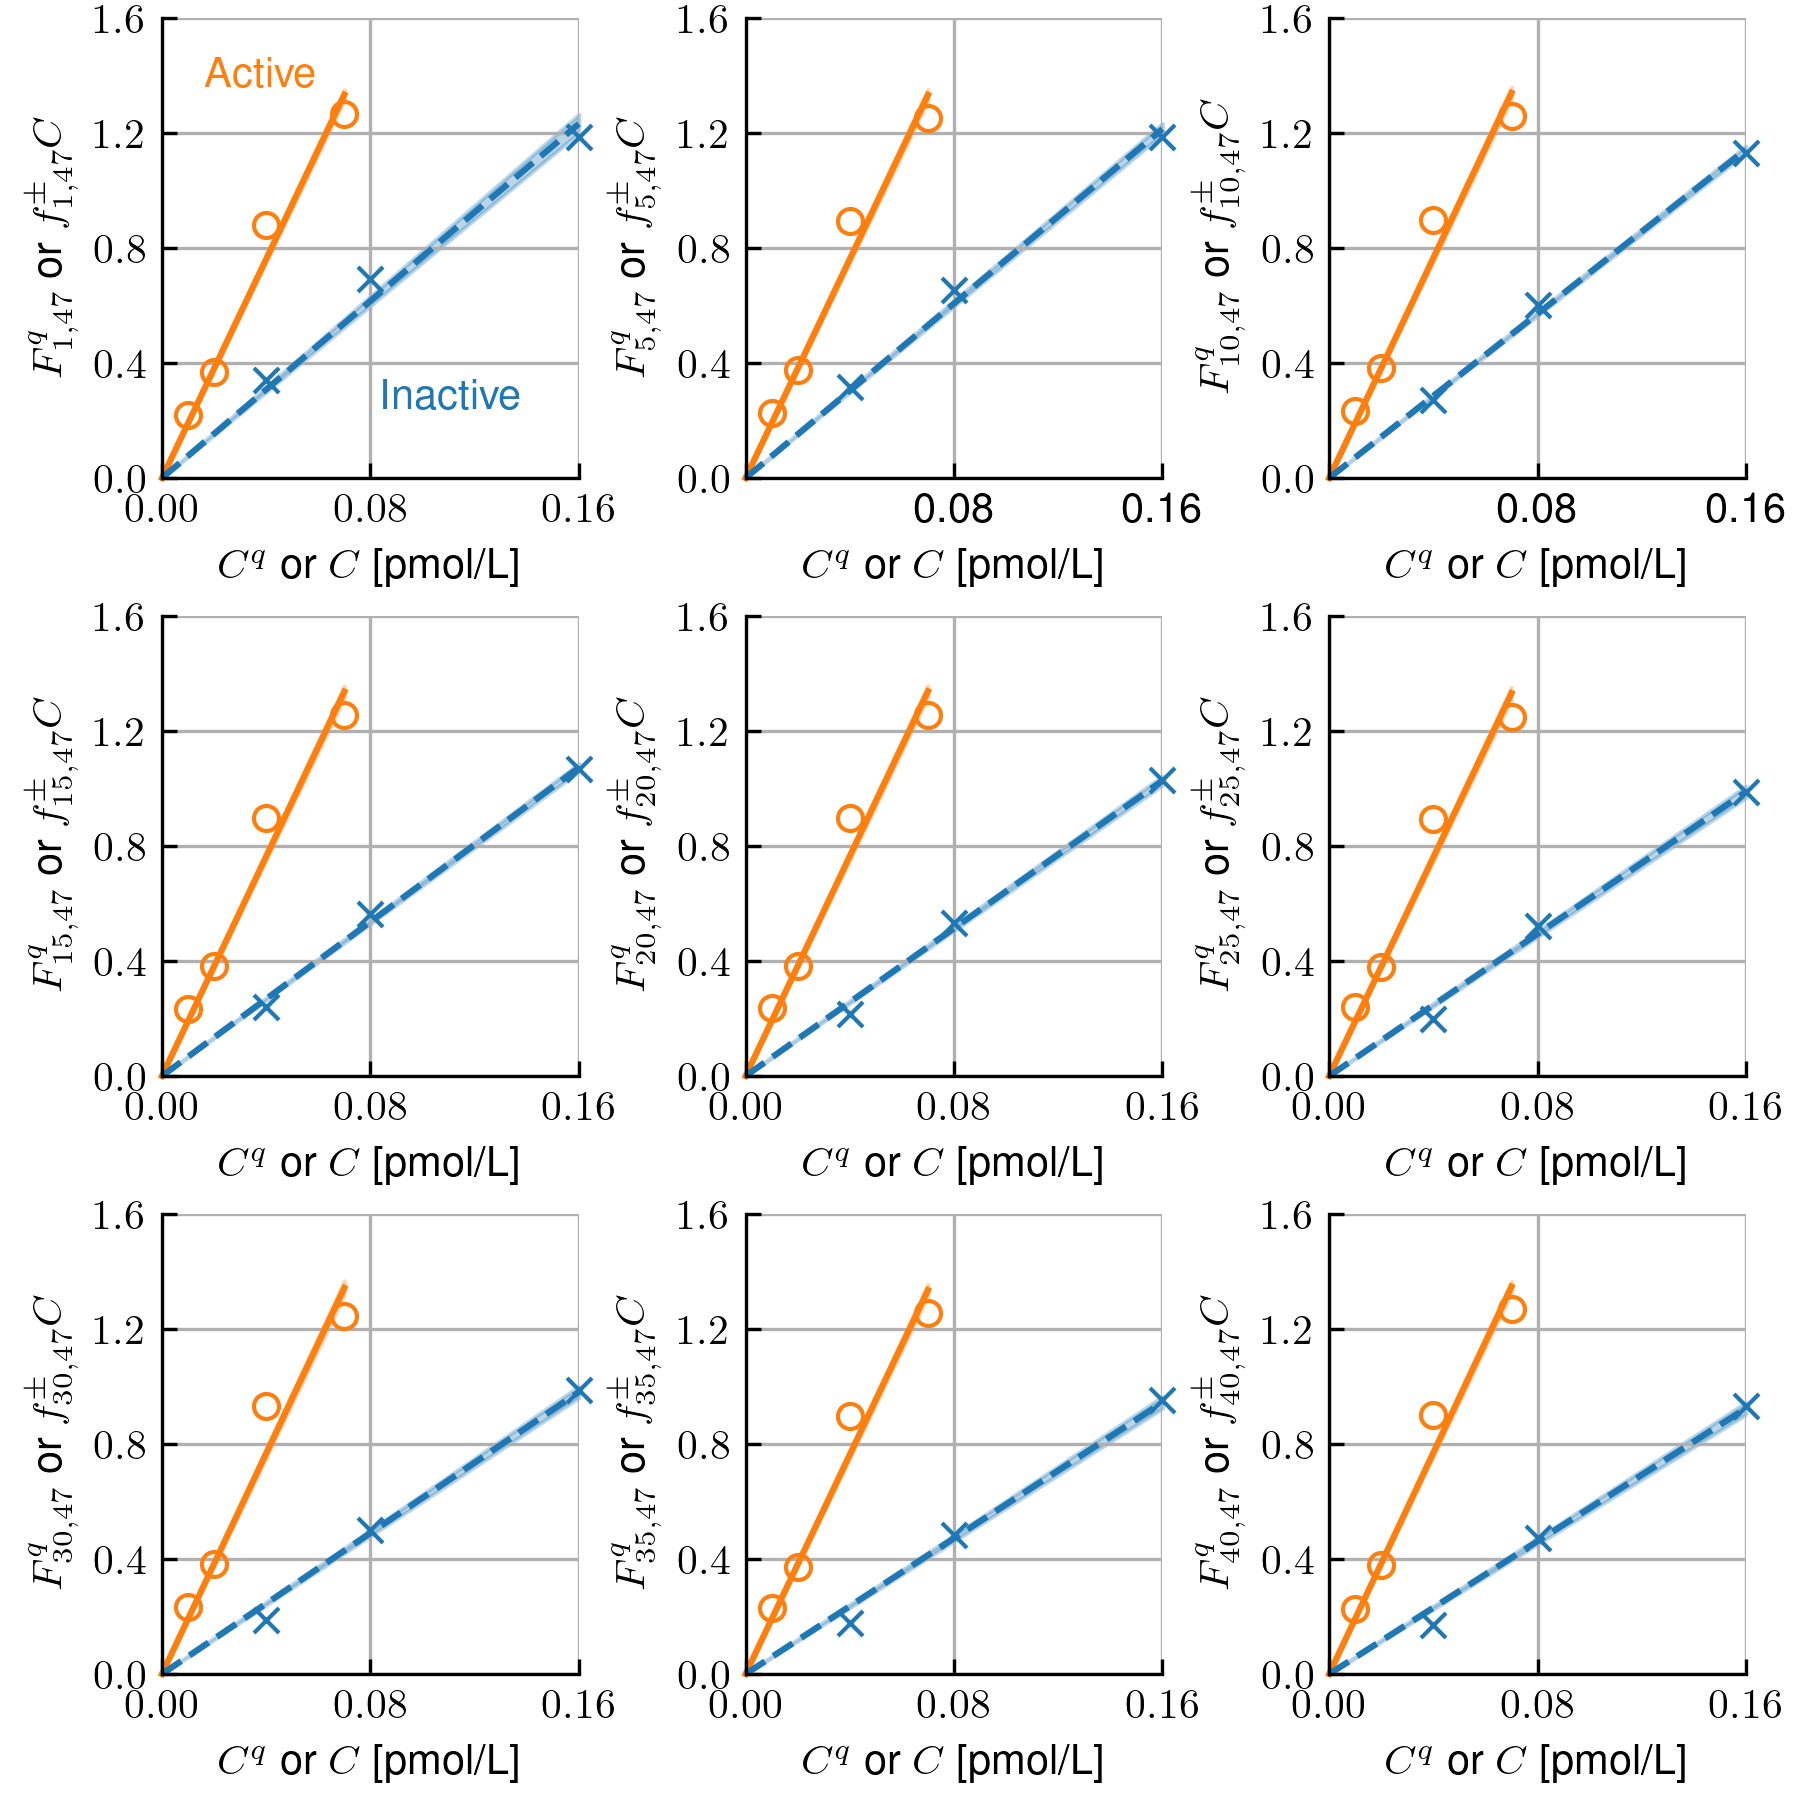
\includegraphics{si-figs/FigS47.png}
                    \caption{
                        As Figure~\ref{fig:S1} with well $w=47$ (or D11).
                    }
                \end{figure}
                \clearpage
    \begin{table}
        \caption{Molar Fluorescence Parameters for Well D11 ($w=47$)}
        \centering
        \begin{tabular}{c|ll|ll}
            Cycle & \multicolumn{2}{c|}{Inactive} & \multicolumn{2}{c}{Active} \\
            \hline
            $i$ & $f_{i,47}^{-}$ & $\sigma_{i,47}^{-}$ &  $f_{i,47}^{+}$ & $\sigma_{i,47}^{+}$ \\
            \hline
    1 & 7.70 & 0.067 & 19.05 & 0.082 \\
2 & 7.63 & 0.066 & 18.68 & 0.083 \\
3 & 7.71 & 0.056 & 18.85 & 0.087 \\
4 & 7.67 & 0.047 & 18.97 & 0.089 \\
5 & 7.59 & 0.039 & 19.03 & 0.091 \\
6 & 7.50 & 0.032 & 19.08 & 0.090 \\
7 & 7.42 & 0.028 & 19.07 & 0.092 \\
8 & 7.30 & 0.028 & 19.10 & 0.093 \\
9 & 7.21 & 0.026 & 19.11 & 0.093 \\
10 & 7.14 & 0.025 & 19.14 & 0.093 \\
11 & 7.04 & 0.025 & 19.19 & 0.093 \\
12 & 6.91 & 0.028 & 19.13 & 0.091 \\
13 & 6.83 & 0.027 & 19.13 & 0.093 \\
14 & 6.77 & 0.028 & 19.11 & 0.095 \\
15 & 6.70 & 0.028 & 19.10 & 0.094 \\
16 & 6.61 & 0.025 & 19.11 & 0.095 \\
17 & 6.56 & 0.026 & 19.17 & 0.092 \\
18 & 6.50 & 0.028 & 19.22 & 0.093 \\
19 & 6.45 & 0.029 & 19.16 & 0.093 \\
20 & 6.42 & 0.032 & 19.12 & 0.094 \\
21 & 6.39 & 0.036 & 19.10 & 0.094 \\
22 & 6.35 & 0.037 & 19.07 & 0.095 \\
23 & 6.30 & 0.039 & 19.08 & 0.096 \\
24 & 6.24 & 0.041 & 19.07 & 0.098 \\
25 & 6.18 & 0.041 & 19.02 & 0.095 \\
26 & 6.14 & 0.042 & 19.16 & 0.098 \\
27 & 6.12 & 0.040 & 19.2 & 0.11 \\
28 & 6.06 & 0.039 & 19.2 & 0.11 \\
29 & 6.07 & 0.036 & 19.2 & 0.12 \\
30 & 6.13 & 0.041 & 19.2 & 0.11 \\
31 & 6.13 & 0.044 & 19.2 & 0.11 \\
32 & 6.07 & 0.043 & 19.2 & 0.12 \\
33 & 6.04 & 0.042 & 18.95 & 0.096 \\
34 & 5.96 & 0.043 & 19.03 & 0.097 \\
35 & 5.90 & 0.042 & 19.07 & 0.093 \\
36 & 5.80 & 0.041 & 19.10 & 0.093 \\
37 & 5.76 & 0.041 & 19.14 & 0.092 \\
38 & 5.79 & 0.042 & 19.18 & 0.091 \\
39 & 5.82 & 0.044 & 19.17 & 0.092 \\
40 & 5.77 & 0.043 & 19.25 & 0.089 \\
41 & 5.68 & 0.042 & 18.95 & 0.098 \\
42 & 5.59 & 0.040 & 18.8 & 0.10 \\
43 & 5.54 & 0.040 & 18.7 & 0.10 \\
44 & 5.56 & 0.042 & 18.8 & 0.10 \\
45 & 5.56 & 0.045 & 18.8 & 0.10 \\
               \hline
        \end{tabular}
    \end{table}
    \clearpage

                \begin{figure}
                    \centering
                    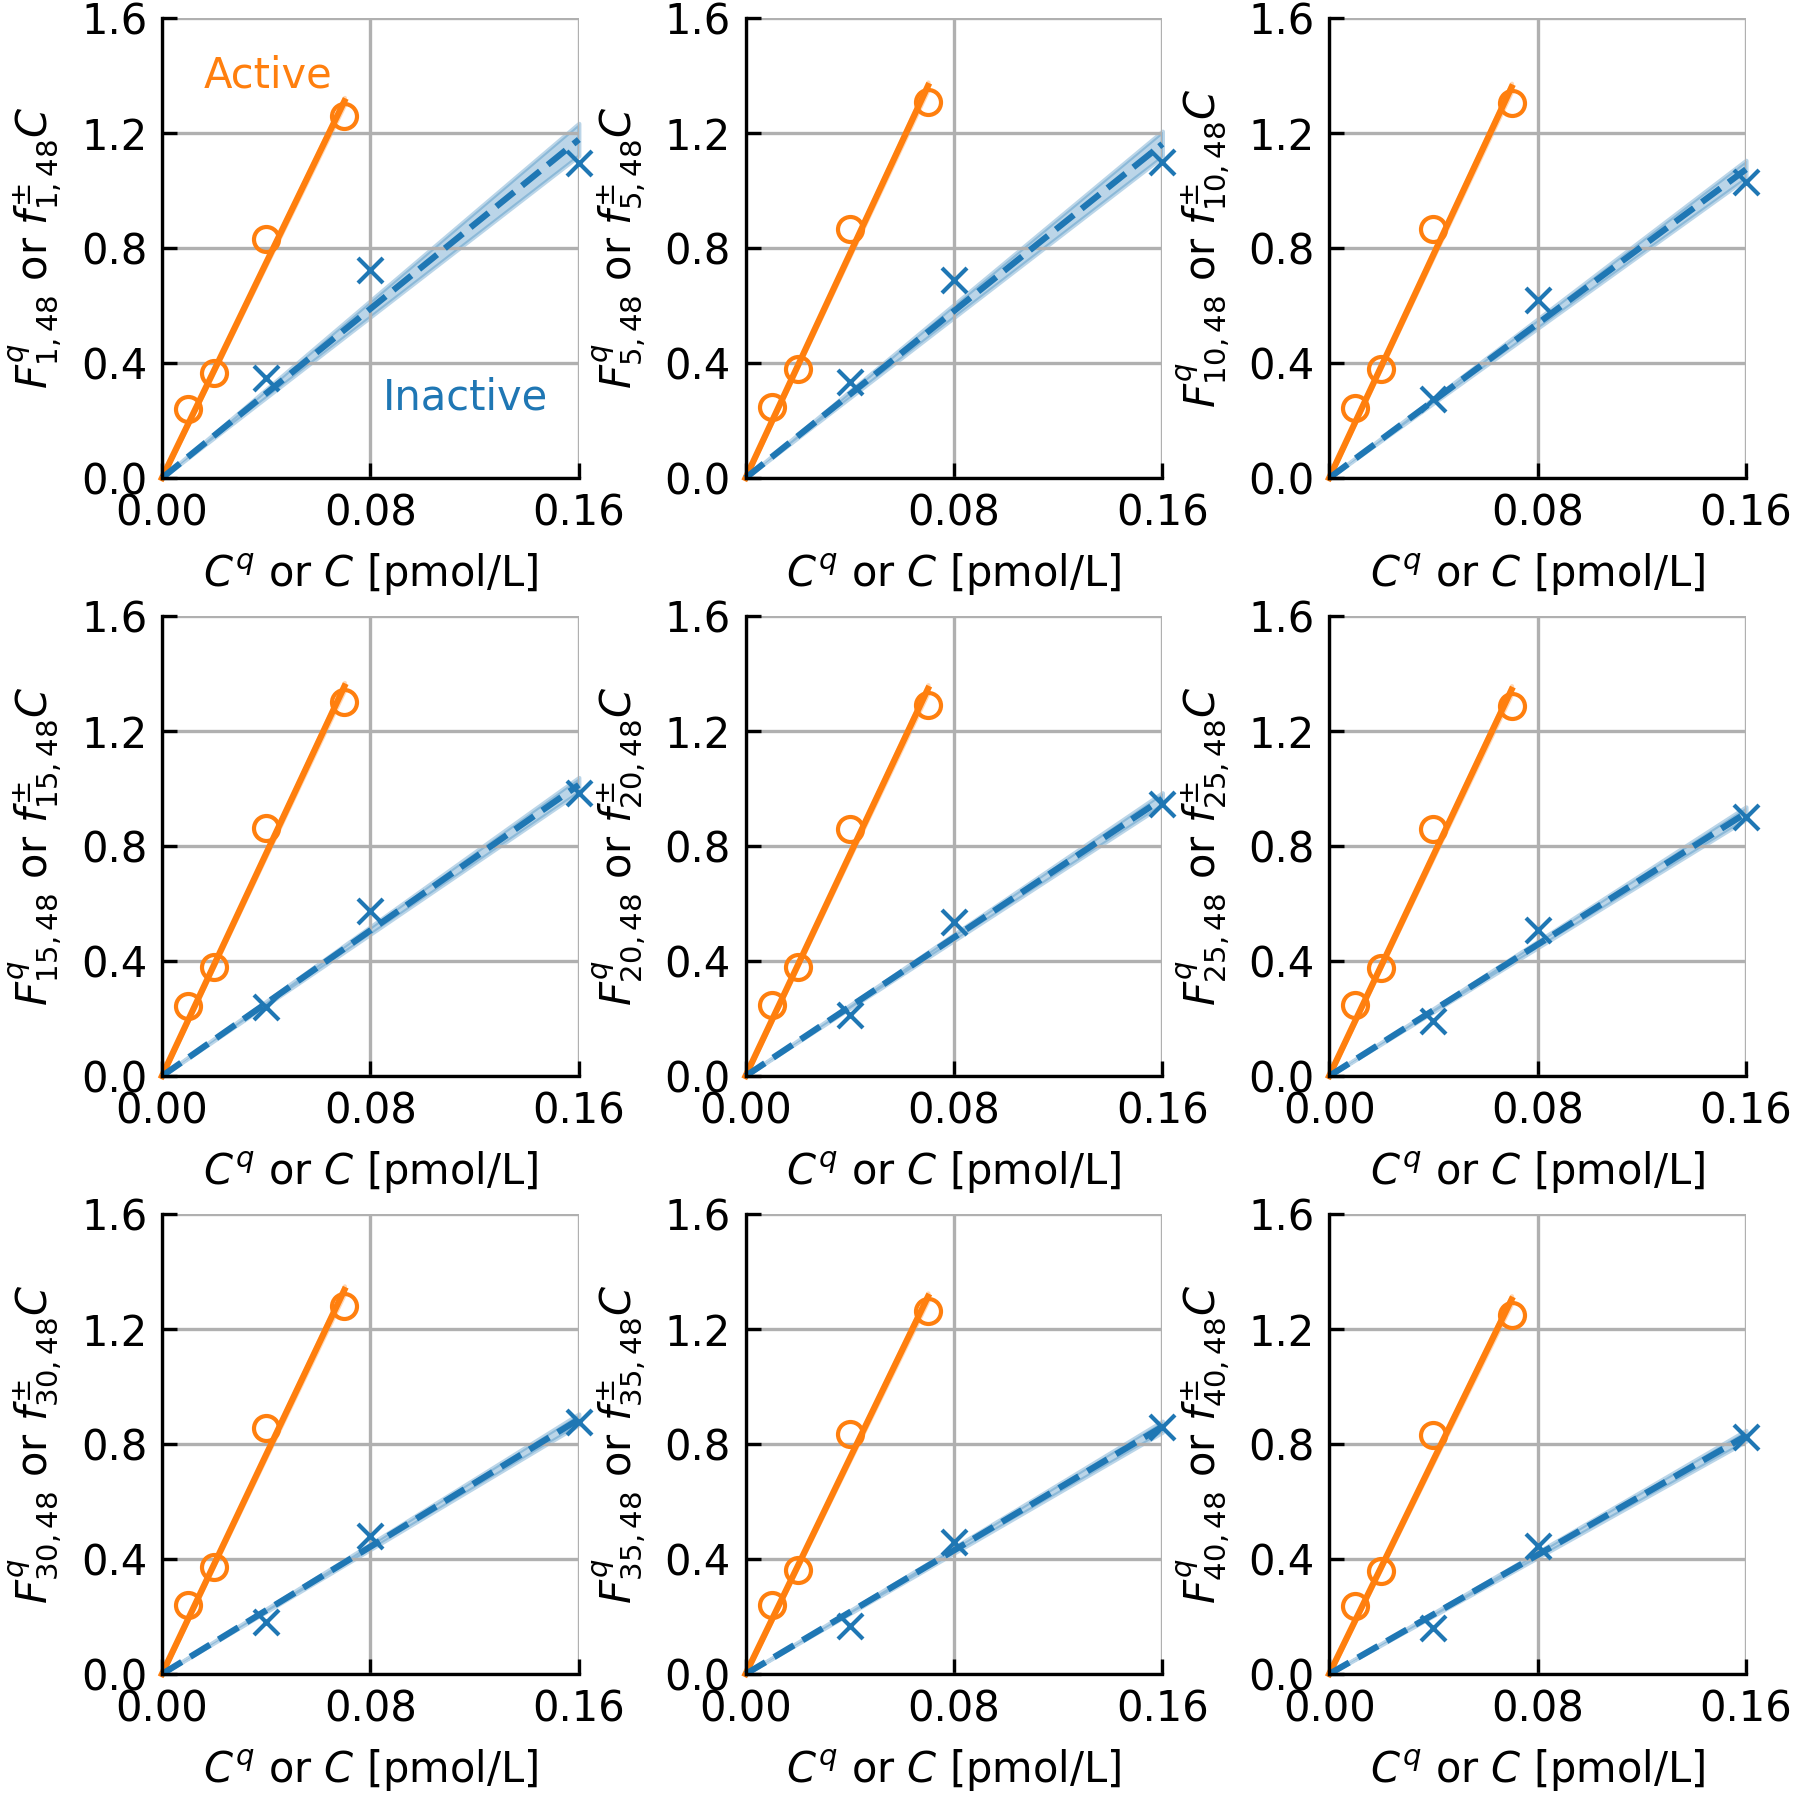
\includegraphics{si-figs/FigS48.png}
                    \caption{
                        As Figure~\ref{fig:S1} with well $w=48$ (or D12).
                    }
                \end{figure}
                \clearpage
    \begin{table}
        \caption{Molar Fluorescence Parameters for Well D12 ($w=48$)}
        \centering
        \begin{tabular}{c|ll|ll}
            Cycle & \multicolumn{2}{c|}{Inactive} & \multicolumn{2}{c}{Active} \\
            \hline
            $i$ & $f_{i,48}^{-}$ & $\sigma_{i,48}^{-}$ &  $f_{i,48}^{+}$ & $\sigma_{i,48}^{+}$ \\
            \hline
    1 & 7.4 & 0.12 & 18.72 & 0.064 \\
2 & 7.4 & 0.12 & 19.11 & 0.065 \\
3 & 7.5 & 0.11 & 19.35 & 0.066 \\
4 & 7.4 & 0.10 & 19.45 & 0.066 \\
5 & 7.26 & 0.093 & 19.48 & 0.067 \\
6 & 7.12 & 0.086 & 19.48 & 0.067 \\
7 & 7.01 & 0.080 & 19.46 & 0.067 \\
8 & 6.90 & 0.074 & 19.45 & 0.068 \\
9 & 6.80 & 0.068 & 19.44 & 0.068 \\
10 & 6.71 & 0.066 & 19.41 & 0.068 \\
11 & 6.65 & 0.062 & 19.43 & 0.070 \\
12 & 6.55 & 0.061 & 19.41 & 0.069 \\
13 & 6.48 & 0.057 & 19.37 & 0.068 \\
14 & 6.37 & 0.058 & 19.41 & 0.070 \\
15 & 6.33 & 0.053 & 19.36 & 0.067 \\
16 & 6.27 & 0.054 & 19.32 & 0.068 \\
17 & 6.19 & 0.052 & 19.28 & 0.068 \\
18 & 6.14 & 0.049 & 19.30 & 0.070 \\
19 & 6.08 & 0.048 & 19.26 & 0.069 \\
20 & 6.02 & 0.044 & 19.24 & 0.069 \\
21 & 5.95 & 0.044 & 19.27 & 0.067 \\
22 & 5.88 & 0.046 & 19.22 & 0.069 \\
23 & 5.82 & 0.045 & 19.29 & 0.067 \\
24 & 5.78 & 0.046 & 19.26 & 0.067 \\
25 & 5.71 & 0.045 & 19.19 & 0.070 \\
26 & 5.70 & 0.044 & 19.22 & 0.068 \\
27 & 5.68 & 0.039 & 19.22 & 0.066 \\
28 & 5.64 & 0.040 & 19.22 & 0.065 \\
29 & 5.59 & 0.040 & 19.14 & 0.072 \\
30 & 5.54 & 0.039 & 19.08 & 0.069 \\
31 & 5.50 & 0.041 & 19.06 & 0.069 \\
32 & 5.47 & 0.045 & 18.89 & 0.073 \\
33 & 5.41 & 0.041 & 18.93 & 0.071 \\
34 & 5.42 & 0.042 & 18.90 & 0.070 \\
35 & 5.38 & 0.040 & 18.75 & 0.064 \\
36 & 5.29 & 0.040 & 18.71 & 0.067 \\
37 & 5.30 & 0.042 & 18.71 & 0.068 \\
38 & 5.26 & 0.041 & 18.74 & 0.064 \\
39 & 5.22 & 0.040 & 18.66 & 0.066 \\
40 & 5.18 & 0.040 & 18.60 & 0.066 \\
41 & 5.14 & 0.040 & 18.56 & 0.068 \\
42 & 5.12 & 0.041 & 18.49 & 0.069 \\
43 & 5.10 & 0.039 & 18.52 & 0.069 \\
44 & 5.07 & 0.042 & 18.43 & 0.069 \\
45 & 5.04 & 0.040 & 18.47 & 0.069 \\
               \hline
        \end{tabular}
    \end{table}
    \clearpage

                \begin{figure}
                    \centering
                    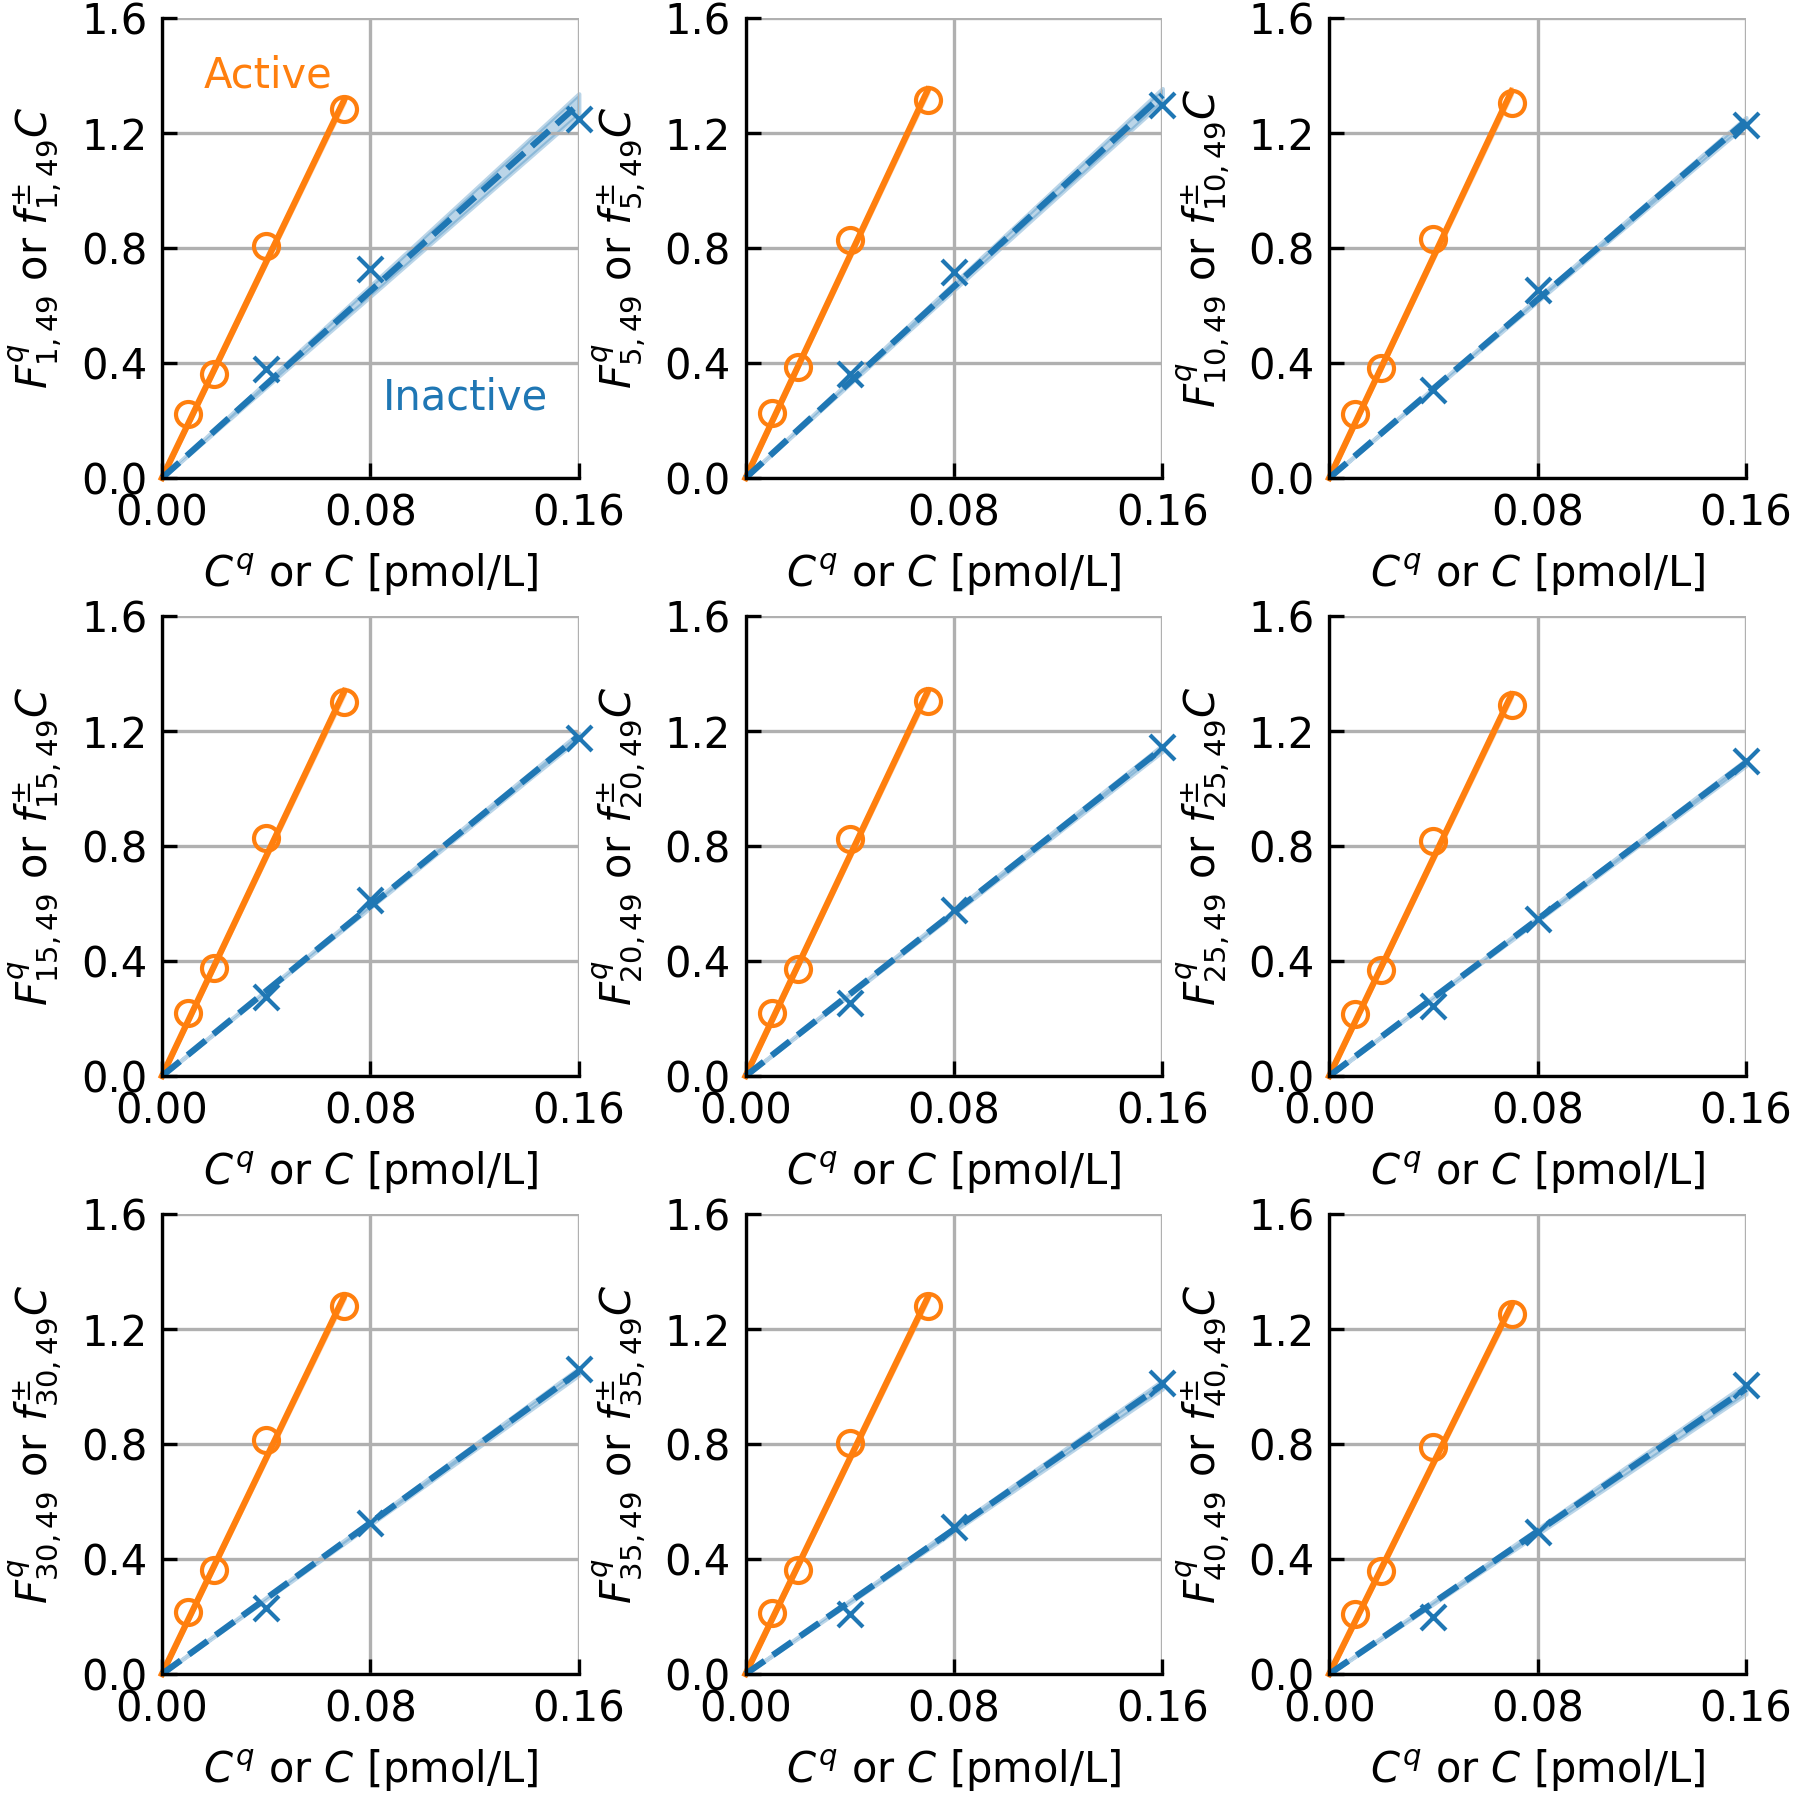
\includegraphics{si-figs/FigS49.png}
                    \caption{
                        As Figure~\ref{fig:S1} with well $w=49$ (or E1).
                    }
                \end{figure}
                \clearpage
    \begin{table}
        \caption{Molar Fluorescence Parameters for Well E1 ($w=49$)}
        \centering
        \begin{tabular}{c|ll|ll}
            Cycle & \multicolumn{2}{c|}{Inactive} & \multicolumn{2}{c}{Active} \\
            \hline
            $i$ & $f_{i,49}^{-}$ & $\sigma_{i,49}^{-}$ &  $f_{i,49}^{+}$ & $\sigma_{i,49}^{+}$ \\
            \hline
    1 & 8.13 & 0.074 & 18.81 & 0.042 \\
2 & 8.56 & 0.066 & 19.02 & 0.039 \\
3 & 8.58 & 0.061 & 19.18 & 0.043 \\
4 & 8.47 & 0.054 & 19.29 & 0.043 \\
5 & 8.32 & 0.047 & 19.30 & 0.043 \\
6 & 8.19 & 0.041 & 19.31 & 0.044 \\
7 & 8.06 & 0.036 & 19.27 & 0.045 \\
8 & 7.95 & 0.032 & 19.28 & 0.045 \\
9 & 7.84 & 0.028 & 19.25 & 0.045 \\
10 & 7.76 & 0.026 & 19.22 & 0.046 \\
11 & 7.70 & 0.023 & 19.21 & 0.045 \\
12 & 7.59 & 0.022 & 19.26 & 0.043 \\
13 & 7.51 & 0.025 & 19.20 & 0.045 \\
14 & 7.42 & 0.024 & 19.14 & 0.046 \\
15 & 7.39 & 0.021 & 19.12 & 0.046 \\
16 & 7.33 & 0.019 & 19.13 & 0.047 \\
17 & 7.26 & 0.019 & 19.15 & 0.043 \\
18 & 7.20 & 0.022 & 19.26 & 0.041 \\
19 & 7.19 & 0.022 & 19.15 & 0.043 \\
20 & 7.12 & 0.023 & 19.14 & 0.043 \\
21 & 7.09 & 0.022 & 19.36 & 0.038 \\
22 & 7.00 & 0.021 & 19.10 & 0.043 \\
23 & 6.92 & 0.020 & 19.11 & 0.049 \\
24 & 6.86 & 0.020 & 19.00 & 0.043 \\
25 & 6.81 & 0.021 & 18.95 & 0.043 \\
26 & 6.71 & 0.021 & 18.88 & 0.043 \\
27 & 6.67 & 0.022 & 18.80 & 0.044 \\
28 & 6.65 & 0.026 & 18.82 & 0.043 \\
29 & 6.61 & 0.025 & 18.74 & 0.044 \\
30 & 6.57 & 0.025 & 18.79 & 0.044 \\
31 & 6.56 & 0.026 & 18.77 & 0.042 \\
32 & 6.55 & 0.029 & 18.70 & 0.044 \\
33 & 6.52 & 0.033 & 18.71 & 0.041 \\
34 & 6.50 & 0.035 & 18.76 & 0.039 \\
35 & 6.29 & 0.030 & 18.73 & 0.040 \\
36 & 6.34 & 0.034 & 18.73 & 0.038 \\
37 & 6.32 & 0.035 & 18.72 & 0.038 \\
38 & 6.30 & 0.037 & 18.71 & 0.038 \\
39 & 6.24 & 0.037 & 18.72 & 0.033 \\
40 & 6.20 & 0.037 & 18.33 & 0.040 \\
41 & 6.18 & 0.038 & 18.34 & 0.042 \\
42 & 6.12 & 0.039 & 18.34 & 0.042 \\
43 & 6.04 & 0.038 & 18.31 & 0.040 \\
44 & 6.02 & 0.040 & 18.30 & 0.039 \\
45 & 6.01 & 0.042 & 18.30 & 0.039 \\
               \hline
        \end{tabular}
    \end{table}
    \clearpage

                \begin{figure}
                    \centering
                    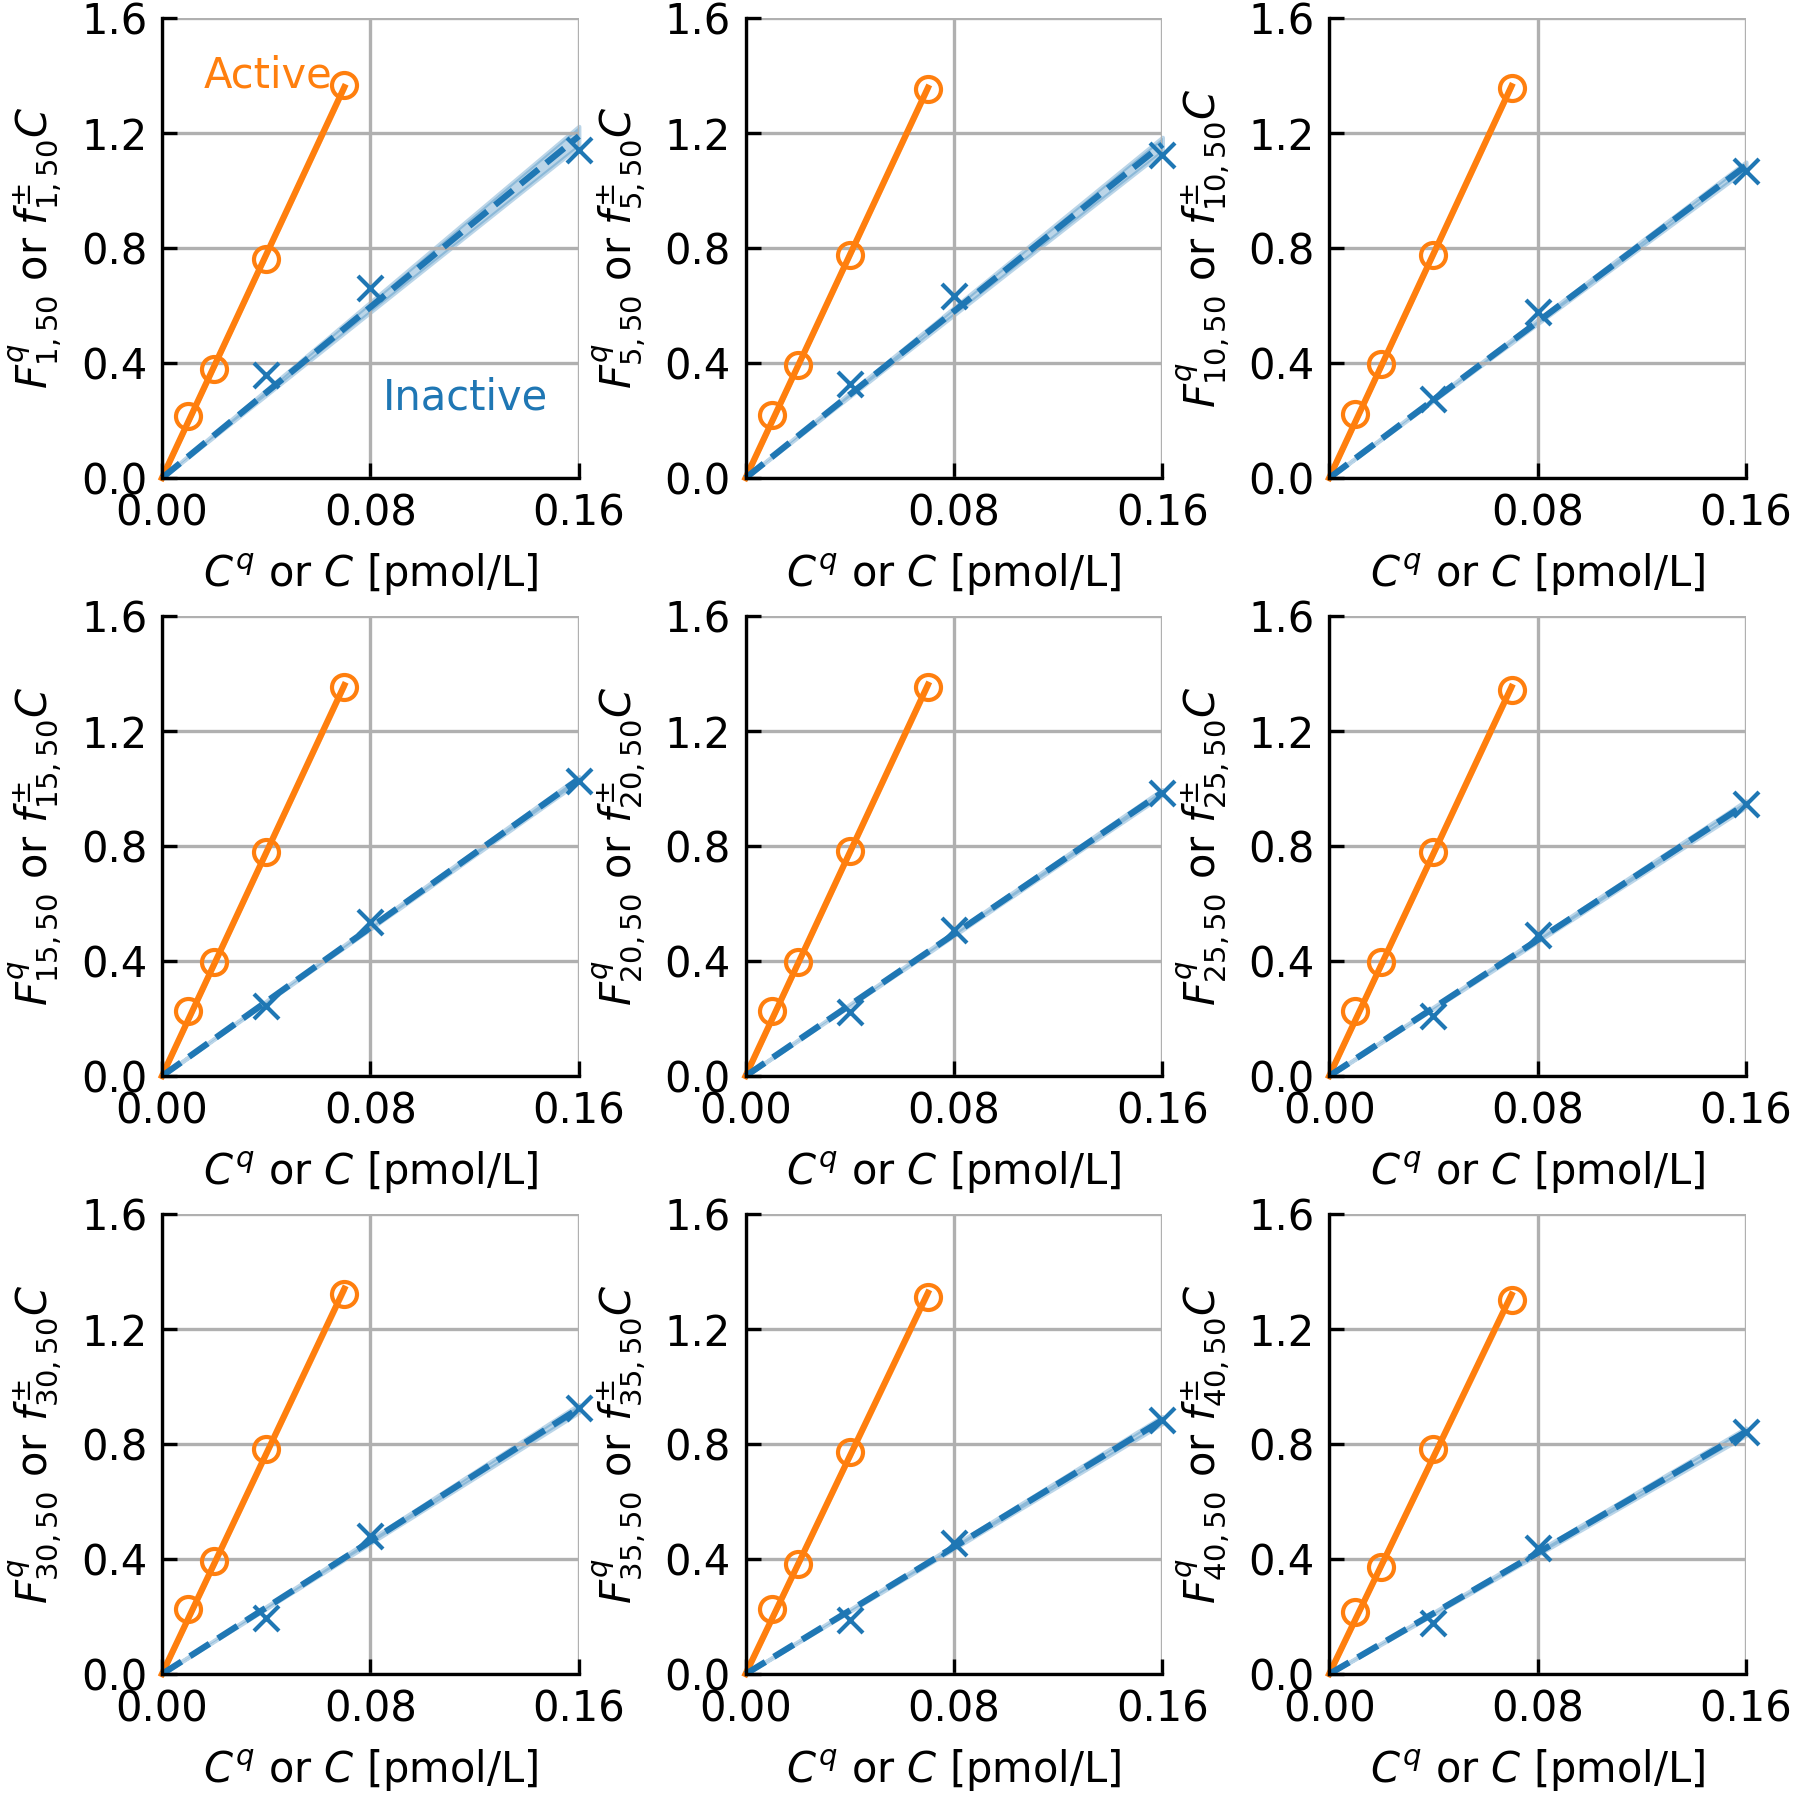
\includegraphics{si-figs/FigS50.png}
                    \caption{
                        As Figure~\ref{fig:S1} with well $w=50$ (or E2).
                    }
                \end{figure}
                \clearpage
    \begin{table}
        \caption{Molar Fluorescence Parameters for Well E2 ($w=50$)}
        \centering
        \begin{tabular}{c|ll|ll}
            Cycle & \multicolumn{2}{c|}{Inactive} & \multicolumn{2}{c}{Active} \\
            \hline
            $i$ & $f_{i,50}^{-}$ & $\sigma_{i,50}^{-}$ &  $f_{i,50}^{+}$ & $\sigma_{i,50}^{+}$ \\
            \hline
    1 & 7.43 & 0.071 & 19.42 & 0.017 \\
2 & 7.49 & 0.065 & 19.16 & 0.014 \\
3 & 7.53 & 0.062 & 19.25 & 0.014 \\
4 & 7.38 & 0.057 & 19.32 & 0.015 \\
5 & 7.25 & 0.052 & 19.39 & 0.016 \\
6 & 7.14 & 0.046 & 19.39 & 0.017 \\
7 & 7.06 & 0.040 & 19.42 & 0.017 \\
8 & 6.95 & 0.034 & 19.43 & 0.017 \\
9 & 6.86 & 0.030 & 19.49 & 0.017 \\
10 & 6.79 & 0.027 & 19.47 & 0.017 \\
11 & 6.68 & 0.027 & 19.44 & 0.017 \\
12 & 6.62 & 0.024 & 19.45 & 0.018 \\
13 & 6.56 & 0.023 & 19.44 & 0.019 \\
14 & 6.53 & 0.023 & 19.44 & 0.018 \\
15 & 6.45 & 0.019 & 19.42 & 0.019 \\
16 & 6.39 & 0.020 & 19.51 & 0.018 \\
17 & 6.28 & 0.020 & 19.54 & 0.018 \\
18 & 6.23 & 0.020 & 19.46 & 0.019 \\
19 & 6.21 & 0.019 & 19.43 & 0.019 \\
20 & 6.17 & 0.020 & 19.44 & 0.019 \\
21 & 6.11 & 0.021 & 19.38 & 0.020 \\
22 & 6.10 & 0.023 & 19.39 & 0.020 \\
23 & 6.05 & 0.020 & 19.44 & 0.019 \\
24 & 6.00 & 0.020 & 19.50 & 0.019 \\
25 & 5.91 & 0.023 & 19.33 & 0.021 \\
26 & 5.93 & 0.025 & 19.28 & 0.022 \\
27 & 5.92 & 0.027 & 19.29 & 0.023 \\
28 & 5.93 & 0.029 & 19.18 & 0.024 \\
29 & 5.83 & 0.028 & 19.12 & 0.026 \\
30 & 5.77 & 0.028 & 19.15 & 0.026 \\
31 & 5.67 & 0.027 & 19.15 & 0.029 \\
32 & 5.63 & 0.028 & 19.13 & 0.027 \\
33 & 5.61 & 0.027 & 19.11 & 0.028 \\
34 & 5.58 & 0.027 & 19.05 & 0.028 \\
35 & 5.52 & 0.025 & 18.95 & 0.025 \\
36 & 5.50 & 0.026 & 18.92 & 0.023 \\
37 & 5.37 & 0.026 & 18.89 & 0.018 \\
38 & 5.34 & 0.026 & 18.92 & 0.021 \\
39 & 5.30 & 0.026 & 18.83 & 0.025 \\
40 & 5.27 & 0.027 & 18.85 & 0.027 \\
41 & 5.24 & 0.026 & 18.87 & 0.028 \\
42 & 5.22 & 0.027 & 18.83 & 0.032 \\
43 & 5.19 & 0.027 & 18.75 & 0.034 \\
44 & 5.16 & 0.027 & 18.73 & 0.037 \\
45 & 5.13 & 0.028 & 18.75 & 0.034 \\
               \hline
        \end{tabular}
    \end{table}
    \clearpage

                \begin{figure}
                    \centering
                    \includegraphics{si-figs/FigS51.png}
                    \caption{
                        As Figure~\ref{fig:S1} with well $w=51$ (or E3).
                    }
                \end{figure}
                \clearpage
    \begin{table}
        \caption{Molar Fluorescence Parameters for Well E3 ($w=51$)}
        \centering
        \begin{tabular}{c|ll|ll}
            Cycle & \multicolumn{2}{c|}{Inactive} & \multicolumn{2}{c}{Active} \\
            \hline
            $i$ & $f_{i,51}^{-}$ & $\sigma_{i,51}^{-}$ &  $f_{i,51}^{+}$ & $\sigma_{i,51}^{+}$ \\
            \hline
    1 & 7.83 & 0.051 & 18.99 & 0.026 \\
2 & 7.83 & 0.053 & 19.12 & 0.027 \\
3 & 7.93 & 0.050 & 19.33 & 0.028 \\
4 & 7.92 & 0.047 & 19.49 & 0.029 \\
5 & 7.86 & 0.041 & 19.59 & 0.029 \\
6 & 7.77 & 0.035 & 19.63 & 0.030 \\
7 & 7.68 & 0.029 & 19.62 & 0.031 \\
8 & 7.60 & 0.024 & 19.62 & 0.030 \\
9 & 7.50 & 0.020 & 19.62 & 0.030 \\
10 & 7.43 & 0.015 & 19.61 & 0.031 \\
11 & 7.35 & 0.011 & 19.58 & 0.031 \\
12 & 7.269 & 0.0089 & 19.56 & 0.032 \\
13 & 7.205 & 0.0068 & 19.54 & 0.033 \\
14 & 7.138 & 0.0058 & 19.53 & 0.034 \\
15 & 7.096 & 0.0056 & 19.52 & 0.036 \\
16 & 7.106 & 0.0092 & 19.43 & 0.040 \\
17 & 7.03 & 0.010 & 19.41 & 0.040 \\
18 & 7.03 & 0.014 & 19.47 & 0.038 \\
19 & 6.96 & 0.016 & 19.64 & 0.035 \\
20 & 6.89 & 0.016 & 19.65 & 0.035 \\
21 & 6.86 & 0.019 & 19.67 & 0.035 \\
22 & 6.79 & 0.019 & 19.78 & 0.035 \\
23 & 6.78 & 0.018 & 19.85 & 0.039 \\
24 & 6.78 & 0.020 & 19.84 & 0.040 \\
25 & 6.76 & 0.021 & 19.84 & 0.039 \\
26 & 6.73 & 0.022 & 19.79 & 0.040 \\
27 & 6.76 & 0.026 & 19.87 & 0.041 \\
28 & 6.72 & 0.028 & 19.83 & 0.040 \\
29 & 6.71 & 0.029 & 19.77 & 0.043 \\
30 & 6.73 & 0.027 & 19.83 & 0.040 \\
31 & 6.65 & 0.031 & 19.76 & 0.044 \\
32 & 6.64 & 0.034 & 19.72 & 0.044 \\
33 & 6.63 & 0.032 & 19.69 & 0.045 \\
34 & 6.55 & 0.038 & 19.63 & 0.046 \\
35 & 6.52 & 0.040 & 19.52 & 0.061 \\
36 & 6.49 & 0.040 & 19.45 & 0.055 \\
37 & 6.51 & 0.042 & 19.27 & 0.057 \\
38 & 6.50 & 0.045 & 19.11 & 0.051 \\
39 & 6.47 & 0.047 & 19.12 & 0.052 \\
40 & 6.08 & 0.022 & 19.05 & 0.051 \\
41 & 6.03 & 0.019 & 19.04 & 0.051 \\
42 & 6.00 & 0.019 & 18.99 & 0.053 \\
43 & 6.01 & 0.020 & 18.92 & 0.049 \\
44 & 6.00 & 0.019 & 18.87 & 0.050 \\
45 & 5.93 & 0.043 & 18.72 & 0.040 \\
               \hline
        \end{tabular}
    \end{table}
    \clearpage

                \begin{figure}
                    \centering
                    \includegraphics{si-figs/FigS52.png}
                    \caption{
                        As Figure~\ref{fig:S1} with well $w=52$ (or E4).
                    }
                \end{figure}
                \clearpage
    \begin{table}
        \caption{Molar Fluorescence Parameters for Well E4 ($w=52$)}
        \centering
        \begin{tabular}{c|ll|ll}
            Cycle & \multicolumn{2}{c|}{Inactive} & \multicolumn{2}{c}{Active} \\
            \hline
            $i$ & $f_{i,52}^{-}$ & $\sigma_{i,52}^{-}$ &  $f_{i,52}^{+}$ & $\sigma_{i,52}^{+}$ \\
            \hline
    1 & 7.62 & 0.092 & 19.19 & 0.031 \\
2 & 7.75 & 0.075 & 18.69 & 0.032 \\
3 & 7.87 & 0.075 & 18.89 & 0.036 \\
4 & 7.82 & 0.073 & 18.97 & 0.038 \\
5 & 7.71 & 0.068 & 19.02 & 0.040 \\
6 & 7.59 & 0.064 & 19.04 & 0.042 \\
7 & 7.47 & 0.061 & 19.10 & 0.042 \\
8 & 7.37 & 0.067 & 19.31 & 0.037 \\
9 & 7.27 & 0.073 & 19.70 & 0.028 \\
10 & 7.16 & 0.076 & 19.81 & 0.029 \\
11 & 7.06 & 0.073 & 19.78 & 0.031 \\
12 & 6.97 & 0.075 & 19.88 & 0.030 \\
13 & 6.89 & 0.079 & 19.94 & 0.030 \\
14 & 6.79 & 0.083 & 19.79 & 0.036 \\
15 & 6.72 & 0.084 & 19.87 & 0.034 \\
16 & 6.63 & 0.086 & 19.97 & 0.034 \\
17 & 6.57 & 0.092 & 20.09 & 0.032 \\
18 & 6.49 & 0.094 & 20.16 & 0.032 \\
19 & 6.39 & 0.089 & 20.22 & 0.031 \\
20 & 6.31 & 0.094 & 20.46 & 0.035 \\
21 & 6.19 & 0.100 & 20.50 & 0.032 \\
22 & 6.1 & 0.10 & 20.52 & 0.032 \\
23 & 6.02 & 0.098 & 20.61 & 0.034 \\
24 & 5.92 & 0.094 & 20.54 & 0.038 \\
25 & 5.9 & 0.10 & 20.55 & 0.038 \\
26 & 5.8 & 0.10 & 20.22 & 0.049 \\
27 & 5.7 & 0.10 & 20.28 & 0.047 \\
28 & 5.6 & 0.10 & 20.31 & 0.046 \\
29 & 5.6 & 0.10 & 20.36 & 0.046 \\
30 & 5.5 & 0.10 & 20.34 & 0.045 \\
31 & 5.46 & 0.099 & 20.21 & 0.049 \\
32 & 5.32 & 0.080 & 20.18 & 0.045 \\
33 & 5.04 & 0.028 & 20.22 & 0.047 \\
34 & 5.14 & 0.061 & 20.26 & 0.047 \\
35 & 5.07 & 0.063 & 20.21 & 0.049 \\
36 & 5.02 & 0.061 & 19.85 & 0.042 \\
37 & 4.94 & 0.060 & 19.70 & 0.041 \\
38 & 4.87 & 0.054 & 19.75 & 0.041 \\
39 & 4.77 & 0.046 & 19.60 & 0.042 \\
40 & 4.70 & 0.040 & 19.55 & 0.043 \\
41 & 4.62 & 0.038 & 17.6 & 0.10 \\
42 & 4.44 & 0.043 & 17.77 & 0.095 \\
43 & 4.42 & 0.042 & 17.63 & 0.080 \\
44 & 4.35 & 0.044 & 17.71 & 0.087 \\
45 & 4.30 & 0.046 & 17.68 & 0.088 \\
               \hline
        \end{tabular}
    \end{table}
    \clearpage

                \begin{figure}
                    \centering
                    \includegraphics{si-figs/FigS53.png}
                    \caption{
                        As Figure~\ref{fig:S1} with well $w=53$ (or E5).
                    }
                \end{figure}
                \clearpage
    \begin{table}
        \caption{Molar Fluorescence Parameters for Well E5 ($w=53$)}
        \centering
        \begin{tabular}{c|ll|ll}
            Cycle & \multicolumn{2}{c|}{Inactive} & \multicolumn{2}{c}{Active} \\
            \hline
            $i$ & $f_{i,53}^{-}$ & $\sigma_{i,53}^{-}$ &  $f_{i,53}^{+}$ & $\sigma_{i,53}^{+}$ \\
            \hline
    1 & 7.60 & 0.078 & 18.85 & 0.017 \\
2 & 7.53 & 0.081 & 18.82 & 0.016 \\
3 & 7.70 & 0.077 & 19.21 & 0.018 \\
4 & 7.67 & 0.074 & 19.39 & 0.019 \\
5 & 7.56 & 0.070 & 19.56 & 0.020 \\
6 & 7.51 & 0.067 & 19.79 & 0.024 \\
7 & 7.44 & 0.063 & 19.88 & 0.022 \\
8 & 7.37 & 0.059 & 20.51 & 0.015 \\
9 & 7.30 & 0.057 & 20.68 & 0.016 \\
10 & 7.22 & 0.056 & 20.83 & 0.017 \\
11 & 7.15 & 0.054 & 20.99 & 0.013 \\
12 & 7.09 & 0.053 & 21.10 & 0.013 \\
13 & 7.02 & 0.052 & 21.27 & 0.014 \\
14 & 7.23 & 0.032 & 21.34 & 0.014 \\
15 & 7.21 & 0.026 & 21.39 & 0.014 \\
16 & 7.16 & 0.022 & 21.47 & 0.014 \\
17 & 7.12 & 0.022 & 21.54 & 0.014 \\
18 & 7.10 & 0.020 & 21.67 & 0.016 \\
19 & 7.07 & 0.019 & 21.54 & 0.012 \\
20 & 7.06 & 0.017 & 21.524 & 0.0097 \\
21 & 7.03 & 0.016 & 21.60 & 0.010 \\
22 & 7.02 & 0.017 & 21.73 & 0.014 \\
23 & 6.99 & 0.016 & 21.77 & 0.012 \\
24 & 6.96 & 0.016 & 21.92 & 0.011 \\
25 & 6.87 & 0.017 & 22.02 & 0.012 \\
26 & 6.72 & 0.020 & 22.05 & 0.010 \\
27 & 6.72 & 0.019 & 22.21 & 0.012 \\
28 & 6.75 & 0.018 & 21.980 & 0.0078 \\
29 & 6.73 & 0.019 & 22.17 & 0.015 \\
30 & 6.72 & 0.020 & 22.04 & 0.019 \\
31 & 6.70 & 0.022 & 22.18 & 0.020 \\
32 & 6.65 & 0.021 & 22.35 & 0.026 \\
33 & 6.64 & 0.025 & 22.39 & 0.025 \\
34 & 6.60 & 0.021 & 22.48 & 0.026 \\
35 & 6.56 & 0.023 & 22.55 & 0.027 \\
36 & 6.55 & 0.024 & 22.59 & 0.027 \\
37 & 6.19 & 0.021 & 22.33 & 0.033 \\
38 & 6.16 & 0.023 & 22.41 & 0.033 \\
39 & 6.12 & 0.021 & 22.48 & 0.034 \\
40 & 6.10 & 0.019 & 22.30 & 0.041 \\
41 & 6.02 & 0.017 & 21.76 & 0.035 \\
42 & 6.00 & 0.018 & 21.82 & 0.035 \\
43 & 5.97 & 0.020 & 21.82 & 0.056 \\
44 & 5.94 & 0.019 & 21.64 & 0.064 \\
45 & 5.83 & 0.020 & 21.59 & 0.063 \\
               \hline
        \end{tabular}
    \end{table}
    \clearpage

                \begin{figure}
                    \centering
                    \includegraphics{si-figs/FigS54.png}
                    \caption{
                        As Figure~\ref{fig:S1} with well $w=54$ (or E6).
                    }
                \end{figure}
                \clearpage
    \begin{table}
        \caption{Molar Fluorescence Parameters for Well E6 ($w=54$)}
        \centering
        \begin{tabular}{c|ll|ll}
            Cycle & \multicolumn{2}{c|}{Inactive} & \multicolumn{2}{c}{Active} \\
            \hline
            $i$ & $f_{i,54}^{-}$ & $\sigma_{i,54}^{-}$ &  $f_{i,54}^{+}$ & $\sigma_{i,54}^{+}$ \\
            \hline
    1 & 6.90 & 0.057 & 17.35 & 0.036 \\
2 & 6.86 & 0.054 & 17.48 & 0.033 \\
3 & 7.01 & 0.054 & 17.64 & 0.035 \\
4 & 7.00 & 0.053 & 17.76 & 0.035 \\
5 & 6.95 & 0.047 & 17.87 & 0.034 \\
6 & 6.90 & 0.038 & 18.00 & 0.030 \\
7 & 6.87 & 0.037 & 18.17 & 0.027 \\
8 & 6.84 & 0.034 & 18.34 & 0.023 \\
9 & 6.78 & 0.032 & 18.43 & 0.020 \\
10 & 6.84 & 0.023 & 18.48 & 0.020 \\
11 & 6.81 & 0.020 & 18.56 & 0.019 \\
12 & 6.85 & 0.014 & 18.69 & 0.021 \\
13 & 6.82 & 0.014 & 18.76 & 0.021 \\
14 & 6.78 & 0.015 & 18.84 & 0.024 \\
15 & 6.73 & 0.016 & 18.96 & 0.025 \\
16 & 6.69 & 0.017 & 19.10 & 0.029 \\
17 & 6.65 & 0.017 & 19.04 & 0.032 \\
18 & 6.61 & 0.013 & 18.97 & 0.035 \\
19 & 6.61 & 0.015 & 18.96 & 0.037 \\
20 & 6.58 & 0.016 & 18.86 & 0.042 \\
21 & 6.53 & 0.017 & 18.82 & 0.046 \\
22 & 6.52 & 0.017 & 18.78 & 0.050 \\
23 & 6.51 & 0.019 & 18.73 & 0.053 \\
24 & 6.47 & 0.020 & 18.66 & 0.056 \\
25 & 6.38 & 0.026 & 18.62 & 0.056 \\
26 & 6.36 & 0.026 & 18.55 & 0.056 \\
27 & 6.34 & 0.029 & 18.50 & 0.057 \\
28 & 6.30 & 0.030 & 18.46 & 0.058 \\
29 & 6.28 & 0.033 & 18.42 & 0.061 \\
30 & 6.24 & 0.033 & 18.39 & 0.062 \\
31 & 6.21 & 0.035 & 18.36 & 0.063 \\
32 & 6.15 & 0.037 & 18.23 & 0.061 \\
33 & 6.13 & 0.040 & 18.18 & 0.064 \\
34 & 6.11 & 0.042 & 18.11 & 0.065 \\
35 & 6.04 & 0.042 & 18.01 & 0.066 \\
36 & 5.93 & 0.040 & 17.82 & 0.077 \\
37 & 5.83 & 0.038 & 17.75 & 0.076 \\
38 & 5.80 & 0.039 & 15.7 & 0.12 \\
39 & 5.77 & 0.039 & 16.1 & 0.11 \\
40 & 5.72 & 0.039 & 15.9 & 0.11 \\
41 & 5.68 & 0.038 & 15.9 & 0.11 \\
42 & 5.65 & 0.041 & 15.8 & 0.11 \\
43 & 5.62 & 0.043 & 14.85 & 0.056 \\
44 & 5.58 & 0.045 & 15.13 & 0.075 \\
45 & 5.55 & 0.047 & 15.07 & 0.073 \\
               \hline
        \end{tabular}
    \end{table}
    \clearpage

                \begin{figure}
                    \centering
                    \includegraphics{si-figs/FigS55.png}
                    \caption{
                        As Figure~\ref{fig:S1} with well $w=55$ (or E7).
                    }
                \end{figure}
                \clearpage
    \begin{table}
        \caption{Molar Fluorescence Parameters for Well E7 ($w=55$)}
        \centering
        \begin{tabular}{c|ll|ll}
            Cycle & \multicolumn{2}{c|}{Inactive} & \multicolumn{2}{c}{Active} \\
            \hline
            $i$ & $f_{i,55}^{-}$ & $\sigma_{i,55}^{-}$ &  $f_{i,55}^{+}$ & $\sigma_{i,55}^{+}$ \\
            \hline
    1 & 8.7 & 0.11 & 20.92 & 0.063 \\
2 & 8.25 & 0.087 & 19.97 & 0.034 \\
3 & 8.35 & 0.083 & 19.98 & 0.038 \\
4 & 8.31 & 0.081 & 19.85 & 0.040 \\
5 & 8.21 & 0.075 & 19.75 & 0.022 \\
6 & 8.14 & 0.069 & 19.67 & 0.017 \\
7 & 8.07 & 0.072 & 19.66 & 0.014 \\
8 & 7.99 & 0.067 & 19.53 & 0.016 \\
9 & 7.93 & 0.064 & 19.55 & 0.016 \\
10 & 7.88 & 0.062 & 19.39 & 0.021 \\
11 & 7.83 & 0.061 & 19.21 & 0.025 \\
12 & 7.77 & 0.059 & 19.16 & 0.024 \\
13 & 7.73 & 0.059 & 19.16 & 0.024 \\
14 & 7.67 & 0.058 & 19.05 & 0.026 \\
15 & 7.60 & 0.057 & 18.97 & 0.029 \\
16 & 7.56 & 0.057 & 18.87 & 0.032 \\
17 & 7.52 & 0.056 & 18.82 & 0.036 \\
18 & 7.46 & 0.056 & 18.80 & 0.040 \\
19 & 7.45 & 0.062 & 18.73 & 0.043 \\
20 & 7.39 & 0.063 & 18.72 & 0.045 \\
21 & 7.36 & 0.062 & 18.89 & 0.066 \\
22 & 7.29 & 0.062 & 18.90 & 0.087 \\
23 & 7.24 & 0.068 & 18.86 & 0.088 \\
24 & 7.21 & 0.066 & 18.89 & 0.087 \\
25 & 7.18 & 0.061 & 18.91 & 0.088 \\
26 & 7.11 & 0.064 & 18.94 & 0.090 \\
27 & 7.14 & 0.065 & 20.47 & 0.054 \\
28 & 7.07 & 0.067 & 20.86 & 0.047 \\
29 & 7.01 & 0.064 & 20.83 & 0.046 \\
30 & 6.98 & 0.064 & 20.83 & 0.046 \\
31 & 7.04 & 0.068 & 20.86 & 0.045 \\
32 & 7.00 & 0.068 & 20.88 & 0.044 \\
33 & 7.03 & 0.056 & 20.88 & 0.044 \\
34 & 7.03 & 0.051 & 20.88 & 0.043 \\
35 & 6.99 & 0.052 & 20.86 & 0.042 \\
36 & 6.96 & 0.053 & 20.90 & 0.048 \\
37 & 6.93 & 0.055 & 20.94 & 0.042 \\
38 & 6.92 & 0.057 & 20.95 & 0.040 \\
39 & 6.91 & 0.055 & 21.09 & 0.037 \\
40 & 6.89 & 0.058 & 21.02 & 0.035 \\
41 & 6.88 & 0.059 & 20.91 & 0.034 \\
42 & 6.88 & 0.066 & 20.91 & 0.033 \\
43 & 6.87 & 0.063 & 20.93 & 0.032 \\
44 & 6.82 & 0.062 & 20.88 & 0.030 \\
45 & 6.71 & 0.057 & 20.80 & 0.028 \\
               \hline
        \end{tabular}
    \end{table}
    \clearpage

                \begin{figure}
                    \centering
                    \includegraphics{si-figs/FigS56.png}
                    \caption{
                        As Figure~\ref{fig:S1} with well $w=56$ (or E8).
                    }
                \end{figure}
                \clearpage
    \begin{table}
        \caption{Molar Fluorescence Parameters for Well E8 ($w=56$)}
        \centering
        \begin{tabular}{c|ll|ll}
            Cycle & \multicolumn{2}{c|}{Inactive} & \multicolumn{2}{c}{Active} \\
            \hline
            $i$ & $f_{i,56}^{-}$ & $\sigma_{i,56}^{-}$ &  $f_{i,56}^{+}$ & $\sigma_{i,56}^{+}$ \\
            \hline
    1 & 7.8 & 0.10 & 18.97 & 0.050 \\
2 & 7.96 & 0.095 & 19.05 & 0.053 \\
3 & 8.16 & 0.097 & 19.33 & 0.057 \\
4 & 8.20 & 0.097 & 19.56 & 0.060 \\
5 & 8.15 & 0.095 & 19.69 & 0.060 \\
6 & 8.23 & 0.079 & 19.76 & 0.061 \\
7 & 8.20 & 0.071 & 19.84 & 0.060 \\
8 & 8.14 & 0.063 & 20.20 & 0.051 \\
9 & 8.11 & 0.056 & 20.35 & 0.047 \\
10 & 8.07 & 0.049 & 20.55 & 0.042 \\
11 & 8.06 & 0.051 & 20.82 & 0.037 \\
12 & 7.98 & 0.050 & 21.06 & 0.031 \\
13 & 7.95 & 0.046 & 21.30 & 0.025 \\
14 & 7.92 & 0.041 & 21.46 & 0.021 \\
15 & 7.88 & 0.035 & 21.58 & 0.019 \\
16 & 7.83 & 0.031 & 21.71 & 0.017 \\
17 & 7.78 & 0.030 & 21.69 & 0.017 \\
18 & 7.77 & 0.023 & 21.80 & 0.017 \\
19 & 7.75 & 0.022 & 21.94 & 0.016 \\
20 & 7.76 & 0.025 & 22.15 & 0.020 \\
21 & 7.83 & 0.025 & 22.25 & 0.014 \\
22 & 7.83 & 0.024 & 22.54 & 0.014 \\
23 & 7.81 & 0.025 & 22.28 & 0.028 \\
24 & 7.77 & 0.024 & 22.35 & 0.033 \\
25 & 7.73 & 0.017 & 22.55 & 0.033 \\
26 & 7.71 & 0.016 & 22.67 & 0.032 \\
27 & 7.66 & 0.016 & 22.80 & 0.032 \\
28 & 7.62 & 0.018 & 22.89 & 0.029 \\
29 & 7.60 & 0.018 & 23.00 & 0.026 \\
30 & 7.54 & 0.020 & 23.10 & 0.025 \\
31 & 7.47 & 0.022 & 23.10 & 0.026 \\
32 & 7.47 & 0.022 & 23.20 & 0.023 \\
33 & 7.44 & 0.024 & 23.27 & 0.021 \\
34 & 7.23 & 0.021 & 23.33 & 0.029 \\
35 & 7.21 & 0.021 & 23.28 & 0.027 \\
36 & 6.93 & 0.028 & 23.39 & 0.028 \\
37 & 6.95 & 0.025 & 23.37 & 0.049 \\
38 & 6.87 & 0.015 & 23.27 & 0.048 \\
39 & 6.87 & 0.016 & 23.37 & 0.047 \\
40 & 6.88 & 0.016 & 23.34 & 0.059 \\
41 & 6.84 & 0.015 & 23.34 & 0.059 \\
42 & 6.85 & 0.020 & 23.49 & 0.061 \\
43 & 6.83 & 0.024 & 23.05 & 0.059 \\
44 & 6.83 & 0.022 & 23.07 & 0.059 \\
45 & 6.83 & 0.023 & 23.04 & 0.059 \\
               \hline
        \end{tabular}
    \end{table}
    \clearpage

                \begin{figure}
                    \centering
                    \includegraphics{si-figs/FigS57.png}
                    \caption{
                        As Figure~\ref{fig:S1} with well $w=57$ (or E9).
                    }
                \end{figure}
                \clearpage
    \begin{table}
        \caption{Molar Fluorescence Parameters for Well E9 ($w=57$)}
        \centering
        \begin{tabular}{c|ll|ll}
            Cycle & \multicolumn{2}{c|}{Inactive} & \multicolumn{2}{c}{Active} \\
            \hline
            $i$ & $f_{i,57}^{-}$ & $\sigma_{i,57}^{-}$ &  $f_{i,57}^{+}$ & $\sigma_{i,57}^{+}$ \\
            \hline
    1 & 7.74 & 0.077 & 18.30 & 0.048 \\
2 & 7.75 & 0.075 & 18.31 & 0.041 \\
3 & 7.85 & 0.073 & 18.55 & 0.046 \\
4 & 7.86 & 0.066 & 18.73 & 0.047 \\
5 & 7.83 & 0.055 & 18.86 & 0.045 \\
6 & 7.79 & 0.045 & 18.94 & 0.045 \\
7 & 7.74 & 0.036 & 19.05 & 0.045 \\
8 & 7.65 & 0.030 & 19.08 & 0.043 \\
9 & 7.59 & 0.023 & 19.12 & 0.043 \\
10 & 7.53 & 0.016 & 19.18 & 0.044 \\
11 & 7.47 & 0.012 & 19.23 & 0.046 \\
12 & 7.43 & 0.012 & 19.31 & 0.045 \\
13 & 7.380 & 0.0088 & 19.46 & 0.041 \\
14 & 7.318 & 0.0041 & 19.52 & 0.041 \\
15 & 7.277 & 0.0051 & 19.61 & 0.039 \\
16 & 7.228 & 0.0048 & 19.55 & 0.045 \\
17 & 7.190 & 0.0051 & 19.61 & 0.041 \\
18 & 7.193 & 0.0043 & 19.71 & 0.040 \\
19 & 7.177 & 0.0053 & 19.77 & 0.041 \\
20 & 7.168 & 0.0089 & 19.82 & 0.040 \\
21 & 7.119 & 0.0083 & 19.85 & 0.040 \\
22 & 7.059 & 0.0100 & 19.88 & 0.037 \\
23 & 7.06 & 0.012 & 19.93 & 0.038 \\
24 & 6.98 & 0.017 & 19.95 & 0.036 \\
25 & 6.748 & 0.0098 & 19.98 & 0.038 \\
26 & 6.68 & 0.017 & 20.05 & 0.036 \\
27 & 6.66 & 0.018 & 20.16 & 0.035 \\
28 & 6.66 & 0.019 & 20.31 & 0.045 \\
29 & 6.65 & 0.019 & 20.08 & 0.024 \\
30 & 6.65 & 0.022 & 20.11 & 0.024 \\
31 & 6.64 & 0.023 & 20.16 & 0.021 \\
32 & 6.64 & 0.026 & 20.08 & 0.022 \\
33 & 6.59 & 0.024 & 20.16 & 0.020 \\
34 & 6.52 & 0.022 & 19.37 & 0.040 \\
35 & 6.50 & 0.024 & 19.43 & 0.040 \\
36 & 6.46 & 0.024 & 19.45 & 0.040 \\
37 & 6.45 & 0.025 & 19.50 & 0.039 \\
38 & 6.41 & 0.026 & 19.07 & 0.053 \\
39 & 6.39 & 0.026 & 19.15 & 0.051 \\
40 & 6.30 & 0.023 & 19.17 & 0.049 \\
41 & 6.22 & 0.023 & 19.20 & 0.048 \\
42 & 5.64 & 0.027 & 19.27 & 0.047 \\
43 & 6.22 & 0.029 & 19.34 & 0.045 \\
44 & 5.92 & 0.014 & 19.36 & 0.046 \\
45 & 5.64 & 0.014 & 19.38 & 0.043 \\
               \hline
        \end{tabular}
    \end{table}
    \clearpage

                \begin{figure}
                    \centering
                    \includegraphics{si-figs/FigS58.png}
                    \caption{
                        As Figure~\ref{fig:S1} with well $w=58$ (or E10).
                    }
                \end{figure}
                \clearpage
    \begin{table}
        \caption{Molar Fluorescence Parameters for Well E10 ($w=58$)}
        \centering
        \begin{tabular}{c|ll|ll}
            Cycle & \multicolumn{2}{c|}{Inactive} & \multicolumn{2}{c}{Active} \\
            \hline
            $i$ & $f_{i,58}^{-}$ & $\sigma_{i,58}^{-}$ &  $f_{i,58}^{+}$ & $\sigma_{i,58}^{+}$ \\
            \hline
    1 & 7.07 & 0.073 & 17.76 & 0.037 \\
2 & 7.32 & 0.062 & 18.03 & 0.035 \\
3 & 7.41 & 0.054 & 18.32 & 0.040 \\
4 & 7.42 & 0.048 & 18.49 & 0.042 \\
5 & 7.37 & 0.040 & 18.67 & 0.041 \\
6 & 7.29 & 0.035 & 18.71 & 0.042 \\
7 & 7.22 & 0.030 & 18.79 & 0.043 \\
8 & 7.20 & 0.027 & 18.86 & 0.042 \\
9 & 7.15 & 0.028 & 18.96 & 0.044 \\
10 & 7.09 & 0.032 & 19.00 & 0.048 \\
11 & 7.03 & 0.034 & 19.03 & 0.047 \\
12 & 6.98 & 0.037 & 19.04 & 0.050 \\
13 & 6.94 & 0.040 & 18.99 & 0.048 \\
14 & 6.91 & 0.043 & 19.02 & 0.050 \\
15 & 6.86 & 0.046 & 19.04 & 0.053 \\
16 & 6.81 & 0.049 & 19.11 & 0.053 \\
17 & 6.78 & 0.053 & 19.09 & 0.054 \\
18 & 6.83 & 0.057 & 19.13 & 0.055 \\
19 & 6.82 & 0.061 & 19.12 & 0.057 \\
20 & 6.81 & 0.065 & 19.12 & 0.058 \\
21 & 6.81 & 0.070 & 19.10 & 0.059 \\
22 & 6.78 & 0.073 & 19.14 & 0.062 \\
23 & 6.71 & 0.071 & 19.23 & 0.061 \\
24 & 6.67 & 0.072 & 19.20 & 0.053 \\
25 & 6.61 & 0.073 & 19.18 & 0.059 \\
26 & 6.55 & 0.074 & 19.25 & 0.060 \\
27 & 6.52 & 0.074 & 19.23 & 0.061 \\
28 & 6.33 & 0.067 & 19.27 & 0.060 \\
29 & 6.21 & 0.064 & 19.38 & 0.059 \\
30 & 6.17 & 0.066 & 19.36 & 0.062 \\
31 & 6.13 & 0.068 & 19.45 & 0.045 \\
32 & 6.14 & 0.068 & 19.60 & 0.045 \\
33 & 6.13 & 0.070 & 19.71 & 0.048 \\
34 & 6.09 & 0.069 & 19.77 & 0.045 \\
35 & 6.08 & 0.070 & 19.62 & 0.037 \\
36 & 5.97 & 0.067 & 19.71 & 0.039 \\
37 & 5.72 & 0.061 & 19.51 & 0.042 \\
38 & 5.70 & 0.064 & 19.74 & 0.041 \\
39 & 5.32 & 0.060 & 19.57 & 0.044 \\
40 & 5.32 & 0.058 & 19.23 & 0.019 \\
41 & 5.31 & 0.058 & 19.24 & 0.021 \\
42 & 5.27 & 0.055 & 19.26 & 0.023 \\
43 & 5.27 & 0.055 & 19.36 & 0.024 \\
44 & 5.26 & 0.055 & 19.34 & 0.027 \\
45 & 5.25 & 0.057 & 19.23 & 0.025 \\
               \hline
        \end{tabular}
    \end{table}
    \clearpage

                \begin{figure}
                    \centering
                    \includegraphics{si-figs/FigS59.png}
                    \caption{
                        As Figure~\ref{fig:S1} with well $w=59$ (or E11).
                    }
                \end{figure}
                \clearpage
    \begin{table}
        \caption{Molar Fluorescence Parameters for Well E11 ($w=59$)}
        \centering
        \begin{tabular}{c|ll|ll}
            Cycle & \multicolumn{2}{c|}{Inactive} & \multicolumn{2}{c}{Active} \\
            \hline
            $i$ & $f_{i,59}^{-}$ & $\sigma_{i,59}^{-}$ &  $f_{i,59}^{+}$ & $\sigma_{i,59}^{+}$ \\
            \hline
    1 & 7.48 & 0.062 & 18.20 & 0.038 \\
2 & 7.70 & 0.040 & 17.68 & 0.044 \\
3 & 7.80 & 0.036 & 17.90 & 0.045 \\
4 & 7.75 & 0.032 & 18.19 & 0.041 \\
5 & 7.67 & 0.026 & 18.39 & 0.037 \\
6 & 7.59 & 0.023 & 18.51 & 0.040 \\
7 & 7.52 & 0.022 & 18.59 & 0.041 \\
8 & 7.45 & 0.024 & 18.67 & 0.041 \\
9 & 7.37 & 0.027 & 18.74 & 0.042 \\
10 & 7.31 & 0.030 & 18.78 & 0.042 \\
11 & 7.24 & 0.033 & 18.83 & 0.040 \\
12 & 7.18 & 0.036 & 18.91 & 0.040 \\
13 & 7.12 & 0.039 & 18.96 & 0.042 \\
14 & 7.07 & 0.042 & 19.04 & 0.047 \\
15 & 7.04 & 0.045 & 19.11 & 0.047 \\
16 & 6.98 & 0.048 & 19.18 & 0.048 \\
17 & 6.93 & 0.050 & 19.26 & 0.046 \\
18 & 6.88 & 0.052 & 19.29 & 0.048 \\
19 & 6.87 & 0.054 & 19.33 & 0.049 \\
20 & 6.81 & 0.056 & 19.35 & 0.050 \\
21 & 6.78 & 0.057 & 19.14 & 0.059 \\
22 & 6.81 & 0.058 & 19.18 & 0.060 \\
23 & 6.82 & 0.062 & 19.12 & 0.064 \\
24 & 6.89 & 0.071 & 19.03 & 0.045 \\
25 & 6.86 & 0.069 & 18.03 & 0.060 \\
26 & 6.59 & 0.057 & 18.02 & 0.060 \\
27 & 6.54 & 0.060 & 18.51 & 0.072 \\
28 & 6.49 & 0.062 & 18.15 & 0.067 \\
29 & 6.45 & 0.063 & 18.19 & 0.068 \\
30 & 6.38 & 0.063 & 18.17 & 0.068 \\
31 & 6.37 & 0.059 & 18.14 & 0.068 \\
32 & 6.34 & 0.061 & 18.10 & 0.070 \\
33 & 6.32 & 0.060 & 17.98 & 0.068 \\
34 & 6.28 & 0.061 & 17.99 & 0.073 \\
35 & 6.25 & 0.062 & 17.75 & 0.069 \\
36 & 6.29 & 0.066 & 17.81 & 0.073 \\
37 & 6.22 & 0.064 & 17.81 & 0.077 \\
38 & 6.21 & 0.066 & 17.84 & 0.081 \\
39 & 6.19 & 0.066 & 17.82 & 0.078 \\
40 & 6.17 & 0.066 & 17.83 & 0.079 \\
41 & 6.17 & 0.068 & 17.73 & 0.082 \\
42 & 6.14 & 0.067 & 17.79 & 0.083 \\
43 & 6.13 & 0.070 & 17.79 & 0.086 \\
44 & 6.11 & 0.072 & 16.68 & 0.056 \\
45 & 5.90 & 0.062 & 17.71 & 0.091 \\
               \hline
        \end{tabular}
    \end{table}
    \clearpage

                \begin{figure}
                    \centering
                    \includegraphics{si-figs/FigS60.png}
                    \caption{
                        As Figure~\ref{fig:S1} with well $w=60$ (or E12).
                    }
                \end{figure}
                \clearpage
    \begin{table}
        \caption{Molar Fluorescence Parameters for Well E12 ($w=60$)}
        \centering
        \begin{tabular}{c|ll|ll}
            Cycle & \multicolumn{2}{c|}{Inactive} & \multicolumn{2}{c}{Active} \\
            \hline
            $i$ & $f_{i,60}^{-}$ & $\sigma_{i,60}^{-}$ &  $f_{i,60}^{+}$ & $\sigma_{i,60}^{+}$ \\
            \hline
    1 & 7.70 & 0.049 & 18.33 & 0.043 \\
2 & 7.81 & 0.045 & 18.25 & 0.046 \\
3 & 7.82 & 0.038 & 18.45 & 0.049 \\
4 & 7.72 & 0.030 & 18.52 & 0.050 \\
5 & 7.60 & 0.022 & 18.55 & 0.050 \\
6 & 7.47 & 0.014 & 18.55 & 0.051 \\
7 & 7.370 & 0.0072 & 18.56 & 0.050 \\
8 & 7.282 & 0.0028 & 18.55 & 0.050 \\
9 & 7.181 & 0.0057 & 18.55 & 0.050 \\
10 & 7.081 & 0.0083 & 18.54 & 0.051 \\
11 & 7.01 & 0.013 & 18.51 & 0.050 \\
12 & 6.94 & 0.017 & 18.53 & 0.049 \\
13 & 6.91 & 0.024 & 18.47 & 0.050 \\
14 & 6.81 & 0.025 & 18.53 & 0.051 \\
15 & 6.74 & 0.028 & 18.45 & 0.053 \\
16 & 6.67 & 0.027 & 18.39 & 0.050 \\
17 & 6.62 & 0.035 & 18.43 & 0.048 \\
18 & 6.53 & 0.035 & 18.40 & 0.051 \\
19 & 6.48 & 0.039 & 18.35 & 0.050 \\
20 & 6.42 & 0.042 & 18.37 & 0.049 \\
21 & 6.37 & 0.043 & 18.30 & 0.049 \\
22 & 6.32 & 0.046 & 18.31 & 0.049 \\
23 & 6.32 & 0.052 & 18.27 & 0.049 \\
24 & 6.26 & 0.055 & 18.37 & 0.050 \\
25 & 6.17 & 0.055 & 18.31 & 0.051 \\
26 & 6.09 & 0.052 & 18.21 & 0.049 \\
27 & 6.04 & 0.055 & 18.18 & 0.048 \\
28 & 5.98 & 0.054 & 18.25 & 0.046 \\
29 & 5.88 & 0.051 & 18.20 & 0.047 \\
30 & 5.84 & 0.052 & 18.30 & 0.043 \\
31 & 5.82 & 0.054 & 18.17 & 0.045 \\
32 & 5.78 & 0.056 & 18.10 & 0.049 \\
33 & 5.76 & 0.057 & 18.02 & 0.051 \\
34 & 5.76 & 0.058 & 17.96 & 0.051 \\
35 & 5.73 & 0.058 & 17.79 & 0.057 \\
36 & 5.70 & 0.061 & 17.76 & 0.053 \\
37 & 5.66 & 0.060 & 17.79 & 0.053 \\
38 & 5.63 & 0.060 & 17.78 & 0.052 \\
39 & 5.58 & 0.059 & 17.73 & 0.052 \\
40 & 5.56 & 0.060 & 17.77 & 0.053 \\
41 & 5.53 & 0.062 & 17.66 & 0.049 \\
42 & 5.53 & 0.064 & 17.67 & 0.049 \\
43 & 5.39 & 0.058 & 17.68 & 0.049 \\
44 & 5.39 & 0.060 & 17.61 & 0.045 \\
45 & 5.32 & 0.058 & 17.63 & 0.045 \\
               \hline
        \end{tabular}
    \end{table}
    \clearpage

                \begin{figure}
                    \centering
                    \includegraphics{si-figs/FigS61.png}
                    \caption{
                        As Figure~\ref{fig:S1} with well $w=61$ (or F1).
                    }
                \end{figure}
                \clearpage
    \begin{table}
        \caption{Molar Fluorescence Parameters for Well F1 ($w=61$)}
        \centering
        \begin{tabular}{c|ll|ll}
            Cycle & \multicolumn{2}{c|}{Inactive} & \multicolumn{2}{c}{Active} \\
            \hline
            $i$ & $f_{i,61}^{-}$ & $\sigma_{i,61}^{-}$ &  $f_{i,61}^{+}$ & $\sigma_{i,61}^{+}$ \\
            \hline
    1 & 7.70 & 0.068 & 18.30 & 0.034 \\
2 & 7.94 & 0.063 & 18.67 & 0.036 \\
3 & 8.00 & 0.061 & 18.94 & 0.039 \\
4 & 7.89 & 0.056 & 19.11 & 0.038 \\
5 & 7.71 & 0.050 & 19.19 & 0.039 \\
6 & 7.57 & 0.043 & 19.20 & 0.039 \\
7 & 7.44 & 0.038 & 19.22 & 0.037 \\
8 & 7.33 & 0.034 & 19.20 & 0.037 \\
9 & 7.23 & 0.030 & 19.18 & 0.038 \\
10 & 7.13 & 0.027 & 19.14 & 0.039 \\
11 & 7.05 & 0.025 & 19.16 & 0.038 \\
12 & 6.98 & 0.022 & 19.14 & 0.037 \\
13 & 6.92 & 0.024 & 19.12 & 0.037 \\
14 & 6.83 & 0.024 & 19.11 & 0.038 \\
15 & 6.75 & 0.024 & 19.10 & 0.037 \\
16 & 6.69 & 0.026 & 19.07 & 0.037 \\
17 & 6.62 & 0.025 & 19.07 & 0.036 \\
18 & 6.57 & 0.023 & 19.08 & 0.035 \\
19 & 6.55 & 0.028 & 19.11 & 0.033 \\
20 & 6.49 & 0.029 & 18.99 & 0.036 \\
21 & 6.34 & 0.027 & 18.97 & 0.036 \\
22 & 6.26 & 0.022 & 18.94 & 0.036 \\
23 & 6.20 & 0.023 & 19.02 & 0.037 \\
24 & 6.15 & 0.024 & 18.91 & 0.036 \\
25 & 6.11 & 0.026 & 18.89 & 0.036 \\
26 & 6.05 & 0.025 & 18.87 & 0.035 \\
27 & 6.01 & 0.026 & 18.64 & 0.039 \\
28 & 5.97 & 0.028 & 18.73 & 0.044 \\
29 & 5.93 & 0.028 & 18.56 & 0.031 \\
30 & 5.91 & 0.030 & 18.55 & 0.031 \\
31 & 5.86 & 0.030 & 18.55 & 0.030 \\
32 & 5.82 & 0.032 & 18.53 & 0.030 \\
33 & 5.80 & 0.033 & 18.53 & 0.030 \\
34 & 5.75 & 0.034 & 18.51 & 0.030 \\
35 & 5.72 & 0.034 & 18.48 & 0.033 \\
36 & 5.66 & 0.034 & 18.40 & 0.031 \\
37 & 5.63 & 0.035 & 18.36 & 0.031 \\
38 & 5.60 & 0.036 & 18.36 & 0.032 \\
39 & 5.58 & 0.039 & 18.30 & 0.031 \\
40 & 5.52 & 0.042 & 18.29 & 0.030 \\
41 & 5.49 & 0.043 & 18.28 & 0.030 \\
42 & 5.47 & 0.046 & 18.24 & 0.027 \\
43 & 5.45 & 0.052 & 18.14 & 0.025 \\
44 & 5.21 & 0.040 & 18.14 & 0.026 \\
45 & 5.14 & 0.038 & 18.13 & 0.026 \\
               \hline
        \end{tabular}
    \end{table}
    \clearpage

                \begin{figure}
                    \centering
                    \includegraphics{si-figs/FigS62.png}
                    \caption{
                        As Figure~\ref{fig:S1} with well $w=62$ (or F2).
                    }
                \end{figure}
                \clearpage
    \begin{table}
        \caption{Molar Fluorescence Parameters for Well F2 ($w=62$)}
        \centering
        \begin{tabular}{c|ll|ll}
            Cycle & \multicolumn{2}{c|}{Inactive} & \multicolumn{2}{c}{Active} \\
            \hline
            $i$ & $f_{i,62}^{-}$ & $\sigma_{i,62}^{-}$ &  $f_{i,62}^{+}$ & $\sigma_{i,62}^{+}$ \\
            \hline
    1 & 8.31 & 0.084 & 20.09 & 0.052 \\
2 & 8.54 & 0.075 & 20.05 & 0.064 \\
3 & 8.59 & 0.074 & 20.21 & 0.079 \\
4 & 8.53 & 0.067 & 20.32 & 0.080 \\
5 & 8.39 & 0.061 & 20.35 & 0.082 \\
6 & 8.25 & 0.058 & 20.37 & 0.084 \\
7 & 8.14 & 0.052 & 20.33 & 0.084 \\
8 & 8.03 & 0.048 & 20.34 & 0.084 \\
9 & 7.95 & 0.044 & 20.34 & 0.085 \\
10 & 7.86 & 0.042 & 20.34 & 0.086 \\
11 & 7.78 & 0.039 & 20.30 & 0.086 \\
12 & 7.73 & 0.035 & 20.29 & 0.086 \\
13 & 7.66 & 0.033 & 20.25 & 0.087 \\
14 & 7.59 & 0.032 & 20.17 & 0.089 \\
15 & 7.54 & 0.032 & 20.12 & 0.091 \\
16 & 7.48 & 0.029 & 20.11 & 0.090 \\
17 & 7.38 & 0.029 & 20.19 & 0.089 \\
18 & 7.33 & 0.028 & 20.10 & 0.090 \\
19 & 7.29 & 0.028 & 20.04 & 0.092 \\
20 & 7.24 & 0.027 & 20.08 & 0.091 \\
21 & 7.21 & 0.025 & 20.08 & 0.090 \\
22 & 7.18 & 0.026 & 20.05 & 0.095 \\
23 & 7.16 & 0.021 & 20.00 & 0.096 \\
24 & 7.11 & 0.022 & 20.02 & 0.097 \\
25 & 7.06 & 0.022 & 19.94 & 0.097 \\
26 & 7.06 & 0.023 & 19.92 & 0.099 \\
27 & 7.02 & 0.022 & 19.88 & 0.098 \\
28 & 6.99 & 0.023 & 19.90 & 0.095 \\
29 & 6.93 & 0.023 & 19.86 & 0.095 \\
30 & 6.89 & 0.023 & 19.99 & 0.089 \\
31 & 6.86 & 0.024 & 20.00 & 0.099 \\
32 & 6.82 & 0.024 & 20.0 & 0.10 \\
33 & 6.81 & 0.024 & 19.93 & 0.098 \\
34 & 6.78 & 0.025 & 19.80 & 0.097 \\
35 & 6.72 & 0.026 & 19.70 & 0.097 \\
36 & 6.71 & 0.026 & 19.8 & 0.10 \\
37 & 6.67 & 0.025 & 19.66 & 0.099 \\
38 & 6.64 & 0.025 & 19.65 & 0.096 \\
39 & 6.59 & 0.026 & 19.58 & 0.097 \\
40 & 6.57 & 0.028 & 19.56 & 0.096 \\
41 & 6.61 & 0.028 & 19.54 & 0.096 \\
42 & 6.55 & 0.028 & 19.52 & 0.096 \\
43 & 6.55 & 0.029 & 19.55 & 0.096 \\
44 & 6.50 & 0.030 & 19.55 & 0.096 \\
45 & 6.42 & 0.029 & 19.81 & 0.091 \\
               \hline
        \end{tabular}
    \end{table}
    \clearpage

                \begin{figure}
                    \centering
                    \includegraphics{si-figs/FigS63.png}
                    \caption{
                        As Figure~\ref{fig:S1} with well $w=63$ (or F3).
                    }
                \end{figure}
                \clearpage
    \begin{table}
        \caption{Molar Fluorescence Parameters for Well F3 ($w=63$)}
        \centering
        \begin{tabular}{c|ll|ll}
            Cycle & \multicolumn{2}{c|}{Inactive} & \multicolumn{2}{c}{Active} \\
            \hline
            $i$ & $f_{i,63}^{-}$ & $\sigma_{i,63}^{-}$ &  $f_{i,63}^{+}$ & $\sigma_{i,63}^{+}$ \\
            \hline
    1 & 7.70 & 0.082 & 19.00 & 0.017 \\
2 & 7.80 & 0.079 & 18.96 & 0.017 \\
3 & 7.98 & 0.072 & 19.12 & 0.019 \\
4 & 7.97 & 0.065 & 19.15 & 0.022 \\
5 & 7.89 & 0.059 & 19.20 & 0.024 \\
6 & 7.80 & 0.053 & 19.21 & 0.026 \\
7 & 7.70 & 0.048 & 19.21 & 0.027 \\
8 & 7.59 & 0.044 & 19.17 & 0.028 \\
9 & 7.50 & 0.040 & 19.21 & 0.028 \\
10 & 7.40 & 0.037 & 19.19 & 0.029 \\
11 & 7.31 & 0.034 & 19.18 & 0.031 \\
12 & 7.24 & 0.031 & 19.13 & 0.032 \\
13 & 7.17 & 0.028 & 19.13 & 0.032 \\
14 & 7.10 & 0.025 & 19.14 & 0.031 \\
15 & 7.03 & 0.024 & 19.13 & 0.031 \\
16 & 6.98 & 0.021 & 19.06 & 0.033 \\
17 & 6.92 & 0.019 & 19.13 & 0.032 \\
18 & 6.86 & 0.017 & 19.10 & 0.031 \\
19 & 6.80 & 0.016 & 19.02 & 0.033 \\
20 & 6.75 & 0.015 & 19.01 & 0.034 \\
21 & 6.70 & 0.014 & 18.97 & 0.034 \\
22 & 6.64 & 0.013 & 18.96 & 0.034 \\
23 & 6.58 & 0.012 & 18.93 & 0.035 \\
24 & 6.53 & 0.011 & 18.89 & 0.035 \\
25 & 6.48 & 0.012 & 18.87 & 0.036 \\
26 & 6.44 & 0.011 & 18.85 & 0.037 \\
27 & 6.40 & 0.011 & 18.88 & 0.035 \\
28 & 6.37 & 0.011 & 18.88 & 0.038 \\
29 & 6.34 & 0.012 & 18.83 & 0.038 \\
30 & 6.31 & 0.010 & 18.78 & 0.038 \\
31 & 6.255 & 0.0093 & 18.83 & 0.036 \\
32 & 6.23 & 0.010 & 18.82 & 0.037 \\
33 & 6.21 & 0.010 & 18.83 & 0.036 \\
34 & 6.18 & 0.013 & 18.78 & 0.037 \\
35 & 6.16 & 0.012 & 18.76 & 0.037 \\
36 & 6.11 & 0.011 & 18.99 & 0.031 \\
37 & 6.06 & 0.010 & 18.84 & 0.035 \\
38 & 6.017 & 0.0093 & 18.80 & 0.035 \\
39 & 5.968 & 0.0091 & 18.74 & 0.036 \\
40 & 5.938 & 0.0097 & 18.85 & 0.034 \\
41 & 5.911 & 0.0098 & 18.61 & 0.040 \\
42 & 5.903 & 0.0082 & 18.62 & 0.040 \\
43 & 5.88 & 0.011 & 18.62 & 0.041 \\
44 & 5.86 & 0.012 & 18.61 & 0.040 \\
45 & 5.84 & 0.011 & 18.59 & 0.042 \\
               \hline
        \end{tabular}
    \end{table}
    \clearpage

                \begin{figure}
                    \centering
                    \includegraphics{si-figs/FigS64.png}
                    \caption{
                        As Figure~\ref{fig:S1} with well $w=64$ (or F4).
                    }
                \end{figure}
                \clearpage
    \begin{table}
        \caption{Molar Fluorescence Parameters for Well F4 ($w=64$)}
        \centering
        \begin{tabular}{c|ll|ll}
            Cycle & \multicolumn{2}{c|}{Inactive} & \multicolumn{2}{c}{Active} \\
            \hline
            $i$ & $f_{i,64}^{-}$ & $\sigma_{i,64}^{-}$ &  $f_{i,64}^{+}$ & $\sigma_{i,64}^{+}$ \\
            \hline
    1 & 7.32 & 0.035 & 17.56 & 0.029 \\
2 & 7.41 & 0.030 & 17.30 & 0.037 \\
3 & 7.49 & 0.035 & 17.44 & 0.044 \\
4 & 7.45 & 0.033 & 17.51 & 0.046 \\
5 & 7.37 & 0.029 & 17.57 & 0.047 \\
6 & 7.29 & 0.026 & 17.59 & 0.047 \\
7 & 7.19 & 0.024 & 17.60 & 0.046 \\
8 & 7.11 & 0.022 & 17.60 & 0.046 \\
9 & 7.04 & 0.022 & 17.62 & 0.046 \\
10 & 6.94 & 0.023 & 17.62 & 0.045 \\
11 & 6.87 & 0.023 & 17.61 & 0.044 \\
12 & 6.79 & 0.025 & 17.60 & 0.044 \\
13 & 6.73 & 0.025 & 17.57 & 0.045 \\
14 & 6.65 & 0.026 & 17.57 & 0.045 \\
15 & 6.59 & 0.028 & 17.58 & 0.044 \\
16 & 6.53 & 0.029 & 17.59 & 0.043 \\
17 & 6.49 & 0.031 & 17.58 & 0.044 \\
18 & 6.44 & 0.032 & 17.58 & 0.043 \\
19 & 6.41 & 0.034 & 17.57 & 0.045 \\
20 & 6.36 & 0.036 & 17.59 & 0.046 \\
21 & 6.36 & 0.039 & 17.57 & 0.046 \\
22 & 6.32 & 0.040 & 17.60 & 0.047 \\
23 & 6.33 & 0.043 & 17.73 & 0.043 \\
24 & 6.33 & 0.045 & 17.61 & 0.047 \\
25 & 6.32 & 0.049 & 17.54 & 0.047 \\
26 & 6.30 & 0.051 & 17.78 & 0.046 \\
27 & 6.28 & 0.051 & 17.60 & 0.047 \\
28 & 6.22 & 0.052 & 17.53 & 0.049 \\
29 & 6.21 & 0.055 & 17.44 & 0.050 \\
30 & 6.20 & 0.057 & 17.47 & 0.053 \\
31 & 6.22 & 0.062 & 17.42 & 0.052 \\
32 & 6.10 & 0.058 & 17.47 & 0.050 \\
33 & 6.11 & 0.056 & 17.46 & 0.051 \\
34 & 6.04 & 0.058 & 17.45 & 0.051 \\
35 & 6.03 & 0.059 & 17.46 & 0.052 \\
36 & 6.02 & 0.062 & 17.45 & 0.052 \\
37 & 5.94 & 0.060 & 17.45 & 0.052 \\
38 & 5.89 & 0.059 & 17.33 & 0.063 \\
39 & 5.86 & 0.058 & 17.45 & 0.065 \\
40 & 5.83 & 0.060 & 17.65 & 0.057 \\
41 & 5.81 & 0.062 & 17.70 & 0.057 \\
42 & 5.78 & 0.063 & 17.68 & 0.060 \\
43 & 5.81 & 0.067 & 17.75 & 0.059 \\
44 & 5.70 & 0.062 & 17.70 & 0.060 \\
45 & 5.67 & 0.064 & 17.71 & 0.061 \\
               \hline
        \end{tabular}
    \end{table}
    \clearpage

                \begin{figure}
                    \centering
                    \includegraphics{si-figs/FigS65.png}
                    \caption{
                        As Figure~\ref{fig:S1} with well $w=65$ (or F5).
                    }
                \end{figure}
                \clearpage
    \begin{table}
        \caption{Molar Fluorescence Parameters for Well F5 ($w=65$)}
        \centering
        \begin{tabular}{c|ll|ll}
            Cycle & \multicolumn{2}{c|}{Inactive} & \multicolumn{2}{c}{Active} \\
            \hline
            $i$ & $f_{i,65}^{-}$ & $\sigma_{i,65}^{-}$ &  $f_{i,65}^{+}$ & $\sigma_{i,65}^{+}$ \\
            \hline
    1 & 7.69 & 0.041 & 18.84 & 0.044 \\
2 & 7.65 & 0.056 & 18.38 & 0.041 \\
3 & 7.79 & 0.055 & 18.51 & 0.046 \\
4 & 7.78 & 0.056 & 18.63 & 0.046 \\
5 & 7.67 & 0.055 & 18.69 & 0.045 \\
6 & 7.57 & 0.053 & 18.72 & 0.044 \\
7 & 7.43 & 0.052 & 18.66 & 0.045 \\
8 & 7.30 & 0.052 & 18.59 & 0.046 \\
9 & 7.17 & 0.054 & 18.56 & 0.047 \\
10 & 7.05 & 0.056 & 18.53 & 0.045 \\
11 & 6.92 & 0.058 & 18.48 & 0.044 \\
12 & 6.82 & 0.058 & 18.59 & 0.049 \\
13 & 6.72 & 0.060 & 18.54 & 0.054 \\
14 & 6.62 & 0.061 & 18.53 & 0.058 \\
15 & 6.60 & 0.060 & 18.53 & 0.060 \\
16 & 6.57 & 0.072 & 18.50 & 0.062 \\
17 & 6.53 & 0.078 & 18.53 & 0.064 \\
18 & 6.49 & 0.079 & 18.53 & 0.065 \\
19 & 6.46 & 0.079 & 18.49 & 0.066 \\
20 & 6.43 & 0.081 & 18.51 & 0.069 \\
21 & 6.39 & 0.081 & 18.50 & 0.069 \\
22 & 6.37 & 0.081 & 18.48 & 0.071 \\
23 & 6.33 & 0.082 & 18.51 & 0.070 \\
24 & 6.31 & 0.082 & 18.44 & 0.073 \\
25 & 6.26 & 0.083 & 18.45 & 0.072 \\
26 & 6.24 & 0.083 & 18.38 & 0.076 \\
27 & 6.21 & 0.086 & 18.30 & 0.077 \\
28 & 6.17 & 0.085 & 18.31 & 0.078 \\
29 & 6.14 & 0.086 & 18.28 & 0.076 \\
30 & 6.11 & 0.086 & 18.28 & 0.078 \\
31 & 6.08 & 0.085 & 18.16 & 0.076 \\
32 & 6.01 & 0.086 & 18.13 & 0.078 \\
33 & 5.98 & 0.091 & 18.30 & 0.074 \\
34 & 5.96 & 0.088 & 18.16 & 0.077 \\
35 & 5.84 & 0.067 & 18.10 & 0.077 \\
36 & 5.86 & 0.075 & 18.05 & 0.079 \\
37 & 5.83 & 0.074 & 17.98 & 0.081 \\
38 & 5.80 & 0.071 & 17.96 & 0.082 \\
39 & 5.77 & 0.071 & 17.94 & 0.083 \\
40 & 5.70 & 0.071 & 17.87 & 0.085 \\
41 & 5.67 & 0.067 & 16.74 & 0.029 \\
42 & 5.62 & 0.066 & 16.76 & 0.027 \\
43 & 5.53 & 0.064 & 16.68 & 0.034 \\
44 & 5.49 & 0.065 & 16.60 & 0.035 \\
45 & 5.44 & 0.063 & 16.56 & 0.035 \\
               \hline
        \end{tabular}
    \end{table}
    \clearpage

                \begin{figure}
                    \centering
                    \includegraphics{si-figs/FigS66.png}
                    \caption{
                        As Figure~\ref{fig:S1} with well $w=66$ (or F6).
                    }
                \end{figure}
                \clearpage
    \begin{table}
        \caption{Molar Fluorescence Parameters for Well F6 ($w=66$)}
        \centering
        \begin{tabular}{c|ll|ll}
            Cycle & \multicolumn{2}{c|}{Inactive} & \multicolumn{2}{c}{Active} \\
            \hline
            $i$ & $f_{i,66}^{-}$ & $\sigma_{i,66}^{-}$ &  $f_{i,66}^{+}$ & $\sigma_{i,66}^{+}$ \\
            \hline
    1 & 7.31 & 0.061 & 18.05 & 0.059 \\
2 & 7.24 & 0.078 & 17.66 & 0.063 \\
3 & 7.37 & 0.083 & 17.79 & 0.066 \\
4 & 7.39 & 0.086 & 17.84 & 0.069 \\
5 & 7.32 & 0.085 & 17.90 & 0.070 \\
6 & 7.28 & 0.079 & 17.95 & 0.070 \\
7 & 7.22 & 0.072 & 17.93 & 0.072 \\
8 & 7.17 & 0.068 & 17.91 & 0.073 \\
9 & 7.13 & 0.063 & 17.89 & 0.074 \\
10 & 7.13 & 0.059 & 17.87 & 0.075 \\
11 & 7.13 & 0.056 & 17.84 & 0.076 \\
12 & 7.10 & 0.055 & 17.80 & 0.078 \\
13 & 7.07 & 0.056 & 17.72 & 0.080 \\
14 & 7.09 & 0.054 & 17.69 & 0.081 \\
15 & 7.05 & 0.056 & 17.65 & 0.082 \\
16 & 7.00 & 0.059 & 17.62 & 0.084 \\
17 & 6.98 & 0.060 & 17.62 & 0.086 \\
18 & 6.93 & 0.061 & 17.61 & 0.087 \\
19 & 6.90 & 0.063 & 17.57 & 0.089 \\
20 & 6.91 & 0.066 & 17.71 & 0.085 \\
21 & 6.80 & 0.066 & 17.68 & 0.087 \\
22 & 6.80 & 0.068 & 17.68 & 0.087 \\
23 & 6.74 & 0.068 & 17.65 & 0.091 \\
24 & 6.72 & 0.070 & 17.62 & 0.090 \\
25 & 6.65 & 0.071 & 17.58 & 0.090 \\
26 & 6.63 & 0.073 & 17.56 & 0.092 \\
27 & 6.53 & 0.072 & 17.6 & 0.10 \\
28 & 6.50 & 0.075 & 17.7 & 0.11 \\
29 & 6.45 & 0.076 & 17.7 & 0.11 \\
30 & 6.45 & 0.079 & 17.6 & 0.11 \\
31 & 6.37 & 0.079 & 17.6 & 0.11 \\
32 & 6.32 & 0.080 & 17.6 & 0.12 \\
33 & 6.34 & 0.081 & 17.6 & 0.12 \\
34 & 6.31 & 0.082 & 17.6 & 0.12 \\
35 & 6.31 & 0.081 & 17.6 & 0.12 \\
36 & 5.89 & 0.078 & 17.6 & 0.12 \\
37 & 5.87 & 0.079 & 17.26 & 0.098 \\
38 & 5.86 & 0.082 & 17.3 & 0.11 \\
39 & 5.83 & 0.080 & 17.3 & 0.11 \\
40 & 5.79 & 0.084 & 17.3 & 0.11 \\
41 & 5.0 & 0.10 & 17.0 & 0.11 \\
42 & 4.9 & 0.10 & 16.8 & 0.10 \\
43 & 5.0 & 0.10 & 16.7 & 0.10 \\
44 & 5.0 & 0.10 & 16.7 & 0.10 \\
45 & 4.94 & 0.100 & 16.7 & 0.10 \\
               \hline
        \end{tabular}
    \end{table}
    \clearpage

                \begin{figure}
                    \centering
                    \includegraphics{si-figs/FigS67.png}
                    \caption{
                        As Figure~\ref{fig:S1} with well $w=67$ (or F7).
                    }
                \end{figure}
                \clearpage
    \begin{table}
        \caption{Molar Fluorescence Parameters for Well F7 ($w=67$)}
        \centering
        \begin{tabular}{c|ll|ll}
            Cycle & \multicolumn{2}{c|}{Inactive} & \multicolumn{2}{c}{Active} \\
            \hline
            $i$ & $f_{i,67}^{-}$ & $\sigma_{i,67}^{-}$ &  $f_{i,67}^{+}$ & $\sigma_{i,67}^{+}$ \\
            \hline
    1 & 7.77 & 0.031 & 19.00 & 0.066 \\
2 & 7.65 & 0.038 & 18.59 & 0.070 \\
3 & 7.82 & 0.036 & 18.73 & 0.073 \\
4 & 7.86 & 0.033 & 18.81 & 0.076 \\
5 & 7.80 & 0.027 & 18.94 & 0.075 \\
6 & 7.74 & 0.018 & 18.94 & 0.077 \\
7 & 7.683 & 0.0094 & 18.98 & 0.078 \\
8 & 7.658 & 0.0099 & 19.08 & 0.075 \\
9 & 7.63 & 0.017 & 19.14 & 0.073 \\
10 & 7.57 & 0.023 & 19.27 & 0.074 \\
11 & 7.51 & 0.029 & 19.53 & 0.071 \\
12 & 7.46 & 0.035 & 19.59 & 0.070 \\
13 & 7.40 & 0.039 & 19.67 & 0.069 \\
14 & 7.38 & 0.045 & 19.70 & 0.070 \\
15 & 7.32 & 0.048 & 19.75 & 0.069 \\
16 & 7.28 & 0.052 & 19.82 & 0.069 \\
17 & 7.24 & 0.054 & 19.88 & 0.068 \\
18 & 7.39 & 0.065 & 19.97 & 0.068 \\
19 & 7.41 & 0.070 & 20.04 & 0.066 \\
20 & 7.36 & 0.071 & 20.04 & 0.066 \\
21 & 7.32 & 0.070 & 20.03 & 0.069 \\
22 & 7.30 & 0.070 & 20.11 & 0.068 \\
23 & 7.30 & 0.072 & 20.13 & 0.068 \\
24 & 7.28 & 0.075 & 20.13 & 0.068 \\
25 & 7.29 & 0.081 & 20.18 & 0.069 \\
26 & 7.23 & 0.080 & 20.23 & 0.068 \\
27 & 7.23 & 0.082 & 20.36 & 0.067 \\
28 & 7.20 & 0.083 & 20.42 & 0.067 \\
29 & 7.09 & 0.080 & 20.48 & 0.068 \\
30 & 7.09 & 0.084 & 20.47 & 0.070 \\
31 & 7.06 & 0.084 & 20.20 & 0.082 \\
32 & 7.06 & 0.087 & 20.25 & 0.079 \\
33 & 7.04 & 0.092 & 20.30 & 0.081 \\
34 & 7.04 & 0.093 & 20.26 & 0.077 \\
35 & 6.38 & 0.053 & 20.23 & 0.074 \\
36 & 6.13 & 0.045 & 20.24 & 0.075 \\
37 & 6.14 & 0.049 & 20.28 & 0.075 \\
38 & 5.14 & 0.048 & 20.36 & 0.073 \\
39 & 5.11 & 0.046 & 20.28 & 0.076 \\
40 & 5.09 & 0.044 & 20.28 & 0.077 \\
41 & 5.05 & 0.044 & 20.35 & 0.077 \\
42 & 5.00 & 0.042 & 20.35 & 0.077 \\
43 & 4.98 & 0.040 & 20.36 & 0.077 \\
44 & 4.96 & 0.038 & 20.35 & 0.074 \\
45 & 4.94 & 0.037 & 20.37 & 0.073 \\
               \hline
        \end{tabular}
    \end{table}
    \clearpage

                \begin{figure}
                    \centering
                    \includegraphics{si-figs/FigS68.png}
                    \caption{
                        As Figure~\ref{fig:S1} with well $w=68$ (or F8).
                    }
                \end{figure}
                \clearpage
    \begin{table}
        \caption{Molar Fluorescence Parameters for Well F8 ($w=68$)}
        \centering
        \begin{tabular}{c|ll|ll}
            Cycle & \multicolumn{2}{c|}{Inactive} & \multicolumn{2}{c}{Active} \\
            \hline
            $i$ & $f_{i,68}^{-}$ & $\sigma_{i,68}^{-}$ &  $f_{i,68}^{+}$ & $\sigma_{i,68}^{+}$ \\
            \hline
    1 & 7.28 & 0.065 & 18.00 & 0.038 \\
2 & 7.33 & 0.063 & 17.80 & 0.051 \\
3 & 7.46 & 0.066 & 17.75 & 0.062 \\
4 & 7.43 & 0.068 & 17.82 & 0.065 \\
5 & 7.37 & 0.065 & 17.88 & 0.068 \\
6 & 7.30 & 0.059 & 17.89 & 0.070 \\
7 & 7.24 & 0.055 & 18.09 & 0.067 \\
8 & 7.21 & 0.049 & 18.21 & 0.064 \\
9 & 7.15 & 0.047 & 18.29 & 0.063 \\
10 & 7.10 & 0.045 & 18.33 & 0.063 \\
11 & 7.04 & 0.045 & 18.39 & 0.061 \\
12 & 6.99 & 0.045 & 18.40 & 0.061 \\
13 & 6.96 & 0.046 & 18.42 & 0.060 \\
14 & 6.94 & 0.046 & 18.41 & 0.059 \\
15 & 6.94 & 0.046 & 18.45 & 0.059 \\
16 & 6.90 & 0.046 & 18.48 & 0.057 \\
17 & 6.85 & 0.041 & 18.49 & 0.057 \\
18 & 6.93 & 0.044 & 18.53 & 0.056 \\
19 & 6.89 & 0.045 & 18.52 & 0.056 \\
20 & 6.83 & 0.046 & 18.56 & 0.056 \\
21 & 6.80 & 0.047 & 18.55 & 0.060 \\
22 & 6.75 & 0.046 & 18.58 & 0.057 \\
23 & 6.71 & 0.047 & 18.74 & 0.070 \\
24 & 6.64 & 0.048 & 18.83 & 0.073 \\
25 & 6.59 & 0.047 & 18.84 & 0.074 \\
26 & 6.53 & 0.047 & 18.89 & 0.075 \\
27 & 6.47 & 0.046 & 18.93 & 0.077 \\
28 & 6.41 & 0.045 & 18.95 & 0.078 \\
29 & 6.36 & 0.045 & 18.94 & 0.078 \\
30 & 6.30 & 0.044 & 18.64 & 0.071 \\
31 & 6.24 & 0.044 & 18.11 & 0.028 \\
32 & 5.98 & 0.040 & 18.39 & 0.039 \\
33 & 5.59 & 0.041 & 18.33 & 0.036 \\
34 & 5.71 & 0.035 & 18.25 & 0.033 \\
35 & 5.54 & 0.034 & 18.25 & 0.030 \\
36 & 5.47 & 0.031 & 18.08 & 0.031 \\
37 & 5.38 & 0.032 & 18.01 & 0.031 \\
38 & 5.32 & 0.026 & 17.87 & 0.032 \\
39 & 5.25 & 0.025 & 17.73 & 0.035 \\
40 & 5.14 & 0.024 & 17.60 & 0.031 \\
41 & 5.03 & 0.024 & 17.51 & 0.038 \\
42 & 4.95 & 0.022 & 17.42 & 0.040 \\
43 & 4.88 & 0.020 & 17.41 & 0.042 \\
44 & 4.82 & 0.019 & 17.35 & 0.042 \\
45 & 4.71 & 0.018 & 17.28 & 0.042 \\
               \hline
        \end{tabular}
    \end{table}
    \clearpage

                \begin{figure}
                    \centering
                    \includegraphics{si-figs/FigS69.png}
                    \caption{
                        As Figure~\ref{fig:S1} with well $w=69$ (or F9).
                    }
                \end{figure}
                \clearpage
    \begin{table}
        \caption{Molar Fluorescence Parameters for Well F9 ($w=69$)}
        \centering
        \begin{tabular}{c|ll|ll}
            Cycle & \multicolumn{2}{c|}{Inactive} & \multicolumn{2}{c}{Active} \\
            \hline
            $i$ & $f_{i,69}^{-}$ & $\sigma_{i,69}^{-}$ &  $f_{i,69}^{+}$ & $\sigma_{i,69}^{+}$ \\
            \hline
    1 & 7.26 & 0.051 & 17.25 & 0.041 \\
2 & 7.21 & 0.049 & 17.21 & 0.050 \\
3 & 7.34 & 0.038 & 17.39 & 0.055 \\
4 & 7.34 & 0.031 & 17.50 & 0.058 \\
5 & 7.30 & 0.023 & 17.57 & 0.059 \\
6 & 7.24 & 0.017 & 17.60 & 0.059 \\
7 & 7.19 & 0.012 & 17.60 & 0.061 \\
8 & 7.12 & 0.010 & 17.63 & 0.060 \\
9 & 7.065 & 0.0100 & 17.67 & 0.059 \\
10 & 6.97 & 0.012 & 17.70 & 0.059 \\
11 & 6.90 & 0.014 & 17.73 & 0.057 \\
12 & 6.85 & 0.017 & 17.70 & 0.058 \\
13 & 6.87 & 0.024 & 17.64 & 0.059 \\
14 & 6.83 & 0.027 & 17.65 & 0.059 \\
15 & 6.74 & 0.029 & 17.68 & 0.058 \\
16 & 6.70 & 0.033 & 17.69 & 0.059 \\
17 & 6.65 & 0.036 & 17.70 & 0.057 \\
18 & 6.60 & 0.039 & 17.81 & 0.054 \\
19 & 6.57 & 0.042 & 17.83 & 0.053 \\
20 & 6.49 & 0.041 & 17.80 & 0.054 \\
21 & 6.56 & 0.046 & 17.84 & 0.054 \\
22 & 6.56 & 0.046 & 17.79 & 0.053 \\
23 & 6.50 & 0.048 & 17.80 & 0.053 \\
24 & 6.50 & 0.052 & 17.83 & 0.052 \\
25 & 6.25 & 0.042 & 17.88 & 0.051 \\
26 & 6.27 & 0.046 & 17.66 & 0.060 \\
27 & 6.12 & 0.041 & 17.71 & 0.062 \\
28 & 6.15 & 0.043 & 17.82 & 0.061 \\
29 & 6.11 & 0.043 & 17.90 & 0.061 \\
30 & 6.11 & 0.048 & 17.83 & 0.062 \\
31 & 6.07 & 0.048 & 17.83 & 0.062 \\
32 & 6.06 & 0.049 & 17.93 & 0.061 \\
33 & 6.03 & 0.050 & 17.84 & 0.062 \\
34 & 6.01 & 0.052 & 17.82 & 0.058 \\
35 & 6.01 & 0.052 & 17.87 & 0.059 \\
36 & 6.01 & 0.056 & 17.95 & 0.065 \\
37 & 5.98 & 0.058 & 17.97 & 0.061 \\
38 & 5.98 & 0.063 & 17.59 & 0.061 \\
39 & 5.97 & 0.061 & 17.64 & 0.057 \\
40 & 5.95 & 0.060 & 17.62 & 0.059 \\
41 & 5.95 & 0.061 & 17.54 & 0.061 \\
42 & 5.96 & 0.064 & 17.56 & 0.063 \\
43 & 5.84 & 0.059 & 17.53 & 0.062 \\
44 & 5.86 & 0.061 & 17.63 & 0.061 \\
45 & 5.85 & 0.061 & 17.69 & 0.064 \\
               \hline
        \end{tabular}
    \end{table}
    \clearpage

                \begin{figure}
                    \centering
                    \includegraphics{si-figs/FigS70.png}
                    \caption{
                        As Figure~\ref{fig:S1} with well $w=70$ (or F10).
                    }
                \end{figure}
                \clearpage
    \begin{table}
        \caption{Molar Fluorescence Parameters for Well F10 ($w=70$)}
        \centering
        \begin{tabular}{c|ll|ll}
            Cycle & \multicolumn{2}{c|}{Inactive} & \multicolumn{2}{c}{Active} \\
            \hline
            $i$ & $f_{i,70}^{-}$ & $\sigma_{i,70}^{-}$ &  $f_{i,70}^{+}$ & $\sigma_{i,70}^{+}$ \\
            \hline
    1 & 7.25 & 0.069 & 17.85 & 0.071 \\
2 & 7.28 & 0.071 & 17.59 & 0.079 \\
3 & 7.36 & 0.065 & 17.75 & 0.078 \\
4 & 7.33 & 0.061 & 17.87 & 0.078 \\
5 & 7.25 & 0.057 & 17.93 & 0.078 \\
6 & 7.15 & 0.051 & 17.96 & 0.079 \\
7 & 7.06 & 0.045 & 17.98 & 0.080 \\
8 & 6.97 & 0.041 & 17.98 & 0.079 \\
9 & 6.90 & 0.037 & 18.00 & 0.080 \\
10 & 6.81 & 0.035 & 18.01 & 0.078 \\
11 & 6.74 & 0.032 & 18.04 & 0.077 \\
12 & 6.67 & 0.029 & 18.01 & 0.077 \\
13 & 6.60 & 0.027 & 18.02 & 0.076 \\
14 & 6.55 & 0.025 & 18.03 & 0.075 \\
15 & 6.48 & 0.023 & 18.02 & 0.075 \\
16 & 6.44 & 0.021 & 18.02 & 0.075 \\
17 & 6.38 & 0.019 & 18.02 & 0.075 \\
18 & 6.32 & 0.018 & 18.02 & 0.075 \\
19 & 6.29 & 0.017 & 18.04 & 0.075 \\
20 & 6.24 & 0.017 & 18.02 & 0.076 \\
21 & 6.20 & 0.016 & 18.02 & 0.077 \\
22 & 6.17 & 0.015 & 18.03 & 0.076 \\
23 & 6.13 & 0.015 & 18.08 & 0.077 \\
24 & 6.09 & 0.016 & 18.05 & 0.077 \\
25 & 6.05 & 0.016 & 18.04 & 0.081 \\
26 & 6.02 & 0.017 & 18.03 & 0.080 \\
27 & 5.99 & 0.017 & 18.04 & 0.080 \\
28 & 5.95 & 0.017 & 18.05 & 0.081 \\
29 & 5.93 & 0.017 & 18.01 & 0.082 \\
30 & 5.89 & 0.018 & 18.03 & 0.083 \\
31 & 5.86 & 0.018 & 18.03 & 0.084 \\
32 & 5.82 & 0.020 & 18.16 & 0.081 \\
33 & 5.80 & 0.019 & 18.14 & 0.083 \\
34 & 5.77 & 0.019 & 18.11 & 0.085 \\
35 & 5.73 & 0.020 & 18.09 & 0.089 \\
36 & 5.72 & 0.021 & 18.04 & 0.089 \\
37 & 5.77 & 0.023 & 18.07 & 0.089 \\
38 & 5.75 & 0.024 & 18.07 & 0.091 \\
39 & 5.72 & 0.024 & 18.04 & 0.091 \\
40 & 5.66 & 0.025 & 18.00 & 0.092 \\
41 & 5.67 & 0.026 & 18.01 & 0.093 \\
42 & 5.66 & 0.028 & 18.01 & 0.093 \\
43 & 5.62 & 0.028 & 18.04 & 0.094 \\
44 & 5.62 & 0.029 & 18.05 & 0.095 \\
45 & 5.60 & 0.029 & 18.04 & 0.095 \\
               \hline
        \end{tabular}
    \end{table}
    \clearpage

                \begin{figure}
                    \centering
                    \includegraphics{si-figs/FigS71.png}
                    \caption{
                        As Figure~\ref{fig:S1} with well $w=71$ (or F11).
                    }
                \end{figure}
                \clearpage
    \begin{table}
        \caption{Molar Fluorescence Parameters for Well F11 ($w=71$)}
        \centering
        \begin{tabular}{c|ll|ll}
            Cycle & \multicolumn{2}{c|}{Inactive} & \multicolumn{2}{c}{Active} \\
            \hline
            $i$ & $f_{i,71}^{-}$ & $\sigma_{i,71}^{-}$ &  $f_{i,71}^{+}$ & $\sigma_{i,71}^{+}$ \\
            \hline
    1 & 7.88 & 0.069 & 19.02 & 0.066 \\
2 & 7.84 & 0.073 & 18.91 & 0.062 \\
3 & 7.97 & 0.069 & 19.05 & 0.064 \\
4 & 7.98 & 0.063 & 19.15 & 0.064 \\
5 & 7.93 & 0.056 & 19.20 & 0.065 \\
6 & 7.83 & 0.050 & 19.21 & 0.065 \\
7 & 7.74 & 0.045 & 19.18 & 0.066 \\
8 & 7.66 & 0.040 & 19.16 & 0.066 \\
9 & 7.57 & 0.037 & 19.13 & 0.067 \\
10 & 7.50 & 0.034 & 19.10 & 0.067 \\
11 & 7.43 & 0.032 & 19.11 & 0.068 \\
12 & 7.36 & 0.029 & 19.09 & 0.067 \\
13 & 7.30 & 0.027 & 19.09 & 0.067 \\
14 & 7.25 & 0.025 & 19.04 & 0.068 \\
15 & 7.19 & 0.024 & 18.97 & 0.069 \\
16 & 7.14 & 0.022 & 19.00 & 0.069 \\
17 & 7.09 & 0.022 & 18.98 & 0.069 \\
18 & 7.05 & 0.020 & 18.98 & 0.069 \\
19 & 7.02 & 0.022 & 18.98 & 0.070 \\
20 & 6.99 & 0.020 & 18.97 & 0.070 \\
21 & 6.99 & 0.021 & 18.96 & 0.070 \\
22 & 6.96 & 0.021 & 18.94 & 0.071 \\
23 & 6.91 & 0.022 & 18.91 & 0.072 \\
24 & 6.88 & 0.022 & 18.93 & 0.071 \\
25 & 6.84 & 0.024 & 18.93 & 0.071 \\
26 & 6.79 & 0.026 & 18.91 & 0.072 \\
27 & 6.76 & 0.027 & 18.95 & 0.071 \\
28 & 6.74 & 0.028 & 18.94 & 0.071 \\
29 & 6.74 & 0.030 & 18.93 & 0.072 \\
30 & 6.72 & 0.031 & 18.92 & 0.073 \\
31 & 6.68 & 0.031 & 19.06 & 0.069 \\
32 & 6.73 & 0.035 & 19.02 & 0.070 \\
33 & 6.61 & 0.033 & 18.98 & 0.072 \\
34 & 6.56 & 0.034 & 18.95 & 0.073 \\
35 & 6.53 & 0.035 & 18.94 & 0.076 \\
36 & 6.49 & 0.036 & 18.92 & 0.077 \\
37 & 6.45 & 0.036 & 18.90 & 0.075 \\
38 & 6.44 & 0.037 & 18.89 & 0.074 \\
39 & 6.41 & 0.037 & 18.89 & 0.074 \\
40 & 6.40 & 0.039 & 18.87 & 0.074 \\
41 & 6.37 & 0.039 & 18.95 & 0.073 \\
42 & 6.34 & 0.040 & 18.90 & 0.075 \\
43 & 6.31 & 0.039 & 18.87 & 0.076 \\
44 & 6.31 & 0.040 & 18.84 & 0.078 \\
45 & 6.33 & 0.041 & 19.38 & 0.066 \\
               \hline
        \end{tabular}
    \end{table}
    \clearpage

                \begin{figure}
                    \centering
                    \includegraphics{si-figs/FigS72.png}
                    \caption{
                        As Figure~\ref{fig:S1} with well $w=72$ (or F12).
                    }
                \end{figure}
                \clearpage
    \begin{table}
        \caption{Molar Fluorescence Parameters for Well F12 ($w=72$)}
        \centering
        \begin{tabular}{c|ll|ll}
            Cycle & \multicolumn{2}{c|}{Inactive} & \multicolumn{2}{c}{Active} \\
            \hline
            $i$ & $f_{i,72}^{-}$ & $\sigma_{i,72}^{-}$ &  $f_{i,72}^{+}$ & $\sigma_{i,72}^{+}$ \\
            \hline
    1 & 7.93 & 0.090 & 18.36 & 0.049 \\
2 & 8.19 & 0.078 & 18.51 & 0.054 \\
3 & 8.22 & 0.073 & 18.80 & 0.055 \\
4 & 8.13 & 0.064 & 18.93 & 0.055 \\
5 & 8.00 & 0.056 & 18.98 & 0.054 \\
6 & 7.86 & 0.049 & 18.97 & 0.055 \\
7 & 7.75 & 0.044 & 19.01 & 0.053 \\
8 & 7.65 & 0.039 & 18.99 & 0.054 \\
9 & 7.55 & 0.035 & 18.99 & 0.053 \\
10 & 7.47 & 0.034 & 18.94 & 0.053 \\
11 & 7.38 & 0.031 & 18.99 & 0.052 \\
12 & 7.29 & 0.031 & 18.96 & 0.051 \\
13 & 7.20 & 0.032 & 18.98 & 0.050 \\
14 & 7.13 & 0.031 & 18.94 & 0.051 \\
15 & 7.10 & 0.030 & 18.88 & 0.052 \\
16 & 7.01 & 0.030 & 18.87 & 0.052 \\
17 & 6.93 & 0.031 & 18.87 & 0.054 \\
18 & 6.88 & 0.031 & 18.83 & 0.050 \\
19 & 6.81 & 0.033 & 18.85 & 0.049 \\
20 & 6.74 & 0.035 & 18.77 & 0.051 \\
21 & 6.68 & 0.037 & 18.78 & 0.052 \\
22 & 6.64 & 0.035 & 18.76 & 0.050 \\
23 & 6.57 & 0.035 & 18.79 & 0.051 \\
24 & 6.50 & 0.037 & 18.81 & 0.052 \\
25 & 6.45 & 0.035 & 18.86 & 0.043 \\
26 & 6.40 & 0.039 & 18.75 & 0.045 \\
27 & 6.39 & 0.041 & 18.72 & 0.045 \\
28 & 6.35 & 0.034 & 18.66 & 0.047 \\
29 & 6.33 & 0.036 & 18.68 & 0.046 \\
30 & 6.25 & 0.037 & 18.39 & 0.054 \\
31 & 6.17 & 0.036 & 18.40 & 0.051 \\
32 & 6.18 & 0.039 & 18.43 & 0.051 \\
33 & 6.14 & 0.039 & 18.33 & 0.052 \\
34 & 6.14 & 0.041 & 18.26 & 0.051 \\
35 & 6.07 & 0.041 & 18.23 & 0.051 \\
36 & 6.01 & 0.040 & 18.22 & 0.050 \\
37 & 5.95 & 0.040 & 18.21 & 0.049 \\
38 & 5.92 & 0.042 & 18.14 & 0.048 \\
39 & 5.87 & 0.043 & 18.13 & 0.047 \\
40 & 5.84 & 0.044 & 18.09 & 0.049 \\
41 & 5.80 & 0.045 & 18.03 & 0.042 \\
42 & 5.78 & 0.045 & 17.99 & 0.045 \\
43 & 5.75 & 0.047 & 17.95 & 0.046 \\
44 & 5.72 & 0.047 & 17.95 & 0.046 \\
45 & 5.70 & 0.050 & 17.97 & 0.045 \\
               \hline
        \end{tabular}
    \end{table}
    \clearpage

                \begin{figure}
                    \centering
                    \includegraphics{si-figs/FigS73.png}
                    \caption{
                        As Figure~\ref{fig:S1} with well $w=73$ (or G1).
                    }
                \end{figure}
                \clearpage
    \begin{table}
        \caption{Molar Fluorescence Parameters for Well G1 ($w=73$)}
        \centering
        \begin{tabular}{c|ll|ll}
            Cycle & \multicolumn{2}{c|}{Inactive} & \multicolumn{2}{c}{Active} \\
            \hline
            $i$ & $f_{i,73}^{-}$ & $\sigma_{i,73}^{-}$ &  $f_{i,73}^{+}$ & $\sigma_{i,73}^{+}$ \\
            \hline
    1 & 7.83 & 0.055 & 18.91 & 0.032 \\
2 & 8.13 & 0.043 & 18.91 & 0.032 \\
3 & 8.14 & 0.042 & 18.99 & 0.035 \\
4 & 8.00 & 0.037 & 18.98 & 0.036 \\
5 & 7.84 & 0.032 & 18.97 & 0.036 \\
6 & 7.69 & 0.028 & 18.92 & 0.036 \\
7 & 7.54 & 0.025 & 18.85 & 0.036 \\
8 & 7.41 & 0.024 & 18.80 & 0.037 \\
9 & 7.31 & 0.023 & 18.78 & 0.036 \\
10 & 7.21 & 0.023 & 18.72 & 0.037 \\
11 & 7.12 & 0.024 & 18.70 & 0.035 \\
12 & 7.03 & 0.025 & 18.69 & 0.035 \\
13 & 6.93 & 0.027 & 18.66 & 0.036 \\
14 & 6.87 & 0.030 & 18.63 & 0.035 \\
15 & 6.79 & 0.030 & 18.59 & 0.035 \\
16 & 6.72 & 0.028 & 18.51 & 0.036 \\
17 & 6.67 & 0.030 & 18.54 & 0.035 \\
18 & 6.58 & 0.032 & 18.50 & 0.036 \\
19 & 6.48 & 0.033 & 18.59 & 0.035 \\
20 & 6.41 & 0.034 & 18.48 & 0.036 \\
21 & 6.34 & 0.034 & 18.47 & 0.036 \\
22 & 6.33 & 0.035 & 18.54 & 0.034 \\
23 & 6.24 & 0.039 & 18.43 & 0.037 \\
24 & 6.19 & 0.042 & 18.38 & 0.038 \\
25 & 6.16 & 0.045 & 18.32 & 0.033 \\
26 & 6.04 & 0.038 & 18.23 & 0.033 \\
27 & 5.97 & 0.039 & 18.03 & 0.036 \\
28 & 5.95 & 0.041 & 18.10 & 0.034 \\
29 & 5.89 & 0.043 & 17.99 & 0.038 \\
30 & 5.83 & 0.043 & 18.00 & 0.034 \\
31 & 5.79 & 0.043 & 17.92 & 0.033 \\
32 & 5.76 & 0.044 & 17.90 & 0.033 \\
33 & 5.74 & 0.046 & 17.87 & 0.033 \\
34 & 5.68 & 0.046 & 17.89 & 0.033 \\
35 & 5.61 & 0.045 & 17.85 & 0.033 \\
36 & 5.59 & 0.046 & 17.83 & 0.032 \\
37 & 5.52 & 0.046 & 17.83 & 0.033 \\
38 & 5.36 & 0.044 & 17.83 & 0.033 \\
39 & 5.30 & 0.044 & 17.77 & 0.033 \\
40 & 5.28 & 0.046 & 17.79 & 0.032 \\
41 & 5.26 & 0.048 & 17.78 & 0.031 \\
42 & 5.23 & 0.048 & 17.86 & 0.031 \\
43 & 5.19 & 0.049 & 17.64 & 0.034 \\
44 & 5.19 & 0.052 & 17.62 & 0.031 \\
45 & 5.14 & 0.051 & 17.64 & 0.031 \\
               \hline
        \end{tabular}
    \end{table}
    \clearpage

                \begin{figure}
                    \centering
                    \includegraphics{si-figs/FigS74.png}
                    \caption{
                        As Figure~\ref{fig:S1} with well $w=74$ (or G2).
                    }
                \end{figure}
                \clearpage
    \begin{table}
        \caption{Molar Fluorescence Parameters for Well G2 ($w=74$)}
        \centering
        \begin{tabular}{c|ll|ll}
            Cycle & \multicolumn{2}{c|}{Inactive} & \multicolumn{2}{c}{Active} \\
            \hline
            $i$ & $f_{i,74}^{-}$ & $\sigma_{i,74}^{-}$ &  $f_{i,74}^{+}$ & $\sigma_{i,74}^{+}$ \\
            \hline
    1 & 7.62 & 0.091 & 18.71 & 0.061 \\
2 & 8.02 & 0.079 & 18.54 & 0.062 \\
3 & 8.16 & 0.076 & 18.73 & 0.063 \\
4 & 8.12 & 0.072 & 18.81 & 0.063 \\
5 & 8.02 & 0.067 & 18.90 & 0.062 \\
6 & 7.93 & 0.064 & 18.95 & 0.061 \\
7 & 7.84 & 0.060 & 18.93 & 0.061 \\
8 & 7.74 & 0.058 & 18.97 & 0.064 \\
9 & 7.65 & 0.055 & 18.97 & 0.062 \\
10 & 7.57 & 0.054 & 18.96 & 0.062 \\
11 & 7.49 & 0.052 & 18.96 & 0.062 \\
12 & 7.45 & 0.049 & 18.95 & 0.062 \\
13 & 7.38 & 0.047 & 18.96 & 0.061 \\
14 & 7.30 & 0.047 & 18.95 & 0.061 \\
15 & 7.23 & 0.047 & 18.91 & 0.061 \\
16 & 7.17 & 0.045 & 18.90 & 0.062 \\
17 & 7.10 & 0.044 & 18.90 & 0.061 \\
18 & 7.06 & 0.043 & 19.00 & 0.063 \\
19 & 7.02 & 0.044 & 18.91 & 0.060 \\
20 & 6.97 & 0.043 & 18.85 & 0.060 \\
21 & 6.92 & 0.042 & 18.86 & 0.059 \\
22 & 6.88 & 0.042 & 18.79 & 0.059 \\
23 & 6.85 & 0.041 & 18.80 & 0.059 \\
24 & 6.82 & 0.041 & 18.71 & 0.060 \\
25 & 6.79 & 0.040 & 18.72 & 0.059 \\
26 & 6.74 & 0.040 & 18.81 & 0.057 \\
27 & 6.72 & 0.040 & 18.73 & 0.061 \\
28 & 6.72 & 0.038 & 18.68 & 0.062 \\
29 & 6.66 & 0.040 & 18.62 & 0.061 \\
30 & 6.61 & 0.041 & 18.63 & 0.061 \\
31 & 6.71 & 0.038 & 18.57 & 0.061 \\
32 & 6.56 & 0.042 & 18.61 & 0.062 \\
33 & 6.53 & 0.042 & 18.67 & 0.059 \\
34 & 6.45 & 0.045 & 18.72 & 0.058 \\
35 & 6.47 & 0.045 & 18.59 & 0.060 \\
36 & 6.42 & 0.045 & 18.51 & 0.062 \\
37 & 6.37 & 0.045 & 18.69 & 0.057 \\
38 & 6.40 & 0.047 & 18.53 & 0.061 \\
39 & 6.35 & 0.046 & 18.46 & 0.063 \\
40 & 6.38 & 0.044 & 18.41 & 0.064 \\
41 & 6.26 & 0.047 & 18.36 & 0.065 \\
42 & 6.20 & 0.048 & 18.36 & 0.065 \\
43 & 6.17 & 0.050 & 18.39 & 0.065 \\
44 & 6.12 & 0.049 & 18.37 & 0.066 \\
45 & 6.08 & 0.045 & 18.39 & 0.065 \\
               \hline
        \end{tabular}
    \end{table}
    \clearpage

                \begin{figure}
                    \centering
                    \includegraphics{si-figs/FigS75.png}
                    \caption{
                        As Figure~\ref{fig:S1} with well $w=75$ (or G3).
                    }
                \end{figure}
                \clearpage
    \begin{table}
        \caption{Molar Fluorescence Parameters for Well G3 ($w=75$)}
        \centering
        \begin{tabular}{c|ll|ll}
            Cycle & \multicolumn{2}{c|}{Inactive} & \multicolumn{2}{c}{Active} \\
            \hline
            $i$ & $f_{i,75}^{-}$ & $\sigma_{i,75}^{-}$ &  $f_{i,75}^{+}$ & $\sigma_{i,75}^{+}$ \\
            \hline
    1 & 7.76 & 0.047 & 18.51 & 0.027 \\
2 & 7.94 & 0.054 & 18.51 & 0.024 \\
3 & 8.03 & 0.057 & 18.61 & 0.027 \\
4 & 7.90 & 0.060 & 18.67 & 0.031 \\
5 & 7.78 & 0.057 & 18.63 & 0.033 \\
6 & 7.65 & 0.055 & 18.62 & 0.034 \\
7 & 7.54 & 0.052 & 18.56 & 0.036 \\
8 & 7.44 & 0.049 & 18.54 & 0.036 \\
9 & 7.35 & 0.046 & 18.51 & 0.037 \\
10 & 7.26 & 0.045 & 18.50 & 0.037 \\
11 & 7.16 & 0.043 & 18.48 & 0.037 \\
12 & 7.10 & 0.041 & 18.46 & 0.037 \\
13 & 7.03 & 0.040 & 18.41 & 0.038 \\
14 & 6.98 & 0.037 & 18.40 & 0.037 \\
15 & 6.92 & 0.035 & 18.40 & 0.039 \\
16 & 6.87 & 0.033 & 18.38 & 0.037 \\
17 & 6.81 & 0.033 & 18.40 & 0.037 \\
18 & 6.76 & 0.032 & 18.39 & 0.037 \\
19 & 6.71 & 0.030 & 18.38 & 0.037 \\
20 & 6.66 & 0.029 & 18.44 & 0.035 \\
21 & 6.63 & 0.027 & 18.42 & 0.035 \\
22 & 6.56 & 0.028 & 18.40 & 0.037 \\
23 & 6.54 & 0.026 & 18.35 & 0.036 \\
24 & 6.49 & 0.025 & 18.28 & 0.037 \\
25 & 6.46 & 0.025 & 18.27 & 0.036 \\
26 & 6.43 & 0.024 & 18.25 & 0.037 \\
27 & 6.40 & 0.024 & 18.25 & 0.036 \\
28 & 6.37 & 0.023 & 18.25 & 0.040 \\
29 & 6.34 & 0.022 & 18.23 & 0.038 \\
30 & 6.31 & 0.022 & 18.20 & 0.038 \\
31 & 6.28 & 0.022 & 18.21 & 0.037 \\
32 & 6.25 & 0.022 & 18.19 & 0.035 \\
33 & 6.25 & 0.026 & 18.26 & 0.035 \\
34 & 6.20 & 0.022 & 18.25 & 0.036 \\
35 & 6.21 & 0.021 & 18.25 & 0.036 \\
36 & 6.21 & 0.018 & 18.32 & 0.033 \\
37 & 6.15 & 0.019 & 18.23 & 0.034 \\
38 & 6.08 & 0.019 & 18.21 & 0.033 \\
39 & 6.04 & 0.019 & 18.13 & 0.033 \\
40 & 6.01 & 0.017 & 17.97 & 0.037 \\
41 & 5.97 & 0.021 & 17.92 & 0.038 \\
42 & 5.93 & 0.019 & 17.92 & 0.038 \\
43 & 5.86 & 0.020 & 17.91 & 0.037 \\
44 & 5.84 & 0.018 & 17.89 & 0.038 \\
45 & 5.83 & 0.018 & 17.87 & 0.039 \\
               \hline
        \end{tabular}
    \end{table}
    \clearpage

                \begin{figure}
                    \centering
                    \includegraphics{si-figs/FigS76.png}
                    \caption{
                        As Figure~\ref{fig:S1} with well $w=76$ (or G4).
                    }
                \end{figure}
                \clearpage
    \begin{table}
        \caption{Molar Fluorescence Parameters for Well G4 ($w=76$)}
        \centering
        \begin{tabular}{c|ll|ll}
            Cycle & \multicolumn{2}{c|}{Inactive} & \multicolumn{2}{c}{Active} \\
            \hline
            $i$ & $f_{i,76}^{-}$ & $\sigma_{i,76}^{-}$ &  $f_{i,76}^{+}$ & $\sigma_{i,76}^{+}$ \\
            \hline
    1 & 7.71 & 0.042 & 18.75 & 0.021 \\
2 & 7.82 & 0.055 & 18.70 & 0.031 \\
3 & 7.89 & 0.054 & 18.89 & 0.035 \\
4 & 7.82 & 0.051 & 18.92 & 0.039 \\
5 & 7.72 & 0.047 & 18.95 & 0.041 \\
6 & 7.62 & 0.043 & 18.96 & 0.042 \\
7 & 7.53 & 0.037 & 18.93 & 0.044 \\
8 & 7.43 & 0.034 & 18.91 & 0.045 \\
9 & 7.34 & 0.032 & 18.87 & 0.047 \\
10 & 7.30 & 0.028 & 18.87 & 0.047 \\
11 & 7.24 & 0.026 & 19.04 & 0.046 \\
12 & 7.21 & 0.026 & 19.05 & 0.045 \\
13 & 7.17 & 0.026 & 19.02 & 0.045 \\
14 & 7.12 & 0.027 & 19.04 & 0.045 \\
15 & 7.06 & 0.029 & 19.03 & 0.045 \\
16 & 7.01 & 0.030 & 19.03 & 0.044 \\
17 & 6.95 & 0.031 & 19.13 & 0.042 \\
18 & 6.90 & 0.032 & 19.07 & 0.044 \\
19 & 6.88 & 0.033 & 19.06 & 0.044 \\
20 & 6.84 & 0.036 & 19.05 & 0.044 \\
21 & 6.80 & 0.037 & 19.08 & 0.043 \\
22 & 6.76 & 0.039 & 19.06 & 0.043 \\
23 & 6.72 & 0.041 & 19.06 & 0.044 \\
24 & 6.69 & 0.043 & 19.04 & 0.040 \\
25 & 6.66 & 0.044 & 19.08 & 0.045 \\
26 & 6.63 & 0.046 & 19.06 & 0.044 \\
27 & 6.69 & 0.050 & 19.04 & 0.044 \\
28 & 6.65 & 0.051 & 19.13 & 0.046 \\
29 & 6.52 & 0.047 & 19.10 & 0.047 \\
30 & 6.52 & 0.048 & 19.08 & 0.047 \\
31 & 6.54 & 0.049 & 19.17 & 0.051 \\
32 & 6.43 & 0.046 & 19.11 & 0.046 \\
33 & 6.37 & 0.046 & 19.12 & 0.045 \\
34 & 6.36 & 0.046 & 19.15 & 0.042 \\
35 & 6.32 & 0.047 & 19.06 & 0.042 \\
36 & 6.26 & 0.047 & 19.17 & 0.036 \\
37 & 6.21 & 0.047 & 19.01 & 0.041 \\
38 & 6.18 & 0.048 & 19.03 & 0.040 \\
39 & 6.16 & 0.048 & 19.01 & 0.041 \\
40 & 6.09 & 0.047 & 19.01 & 0.042 \\
41 & 6.05 & 0.048 & 19.00 & 0.041 \\
42 & 6.02 & 0.048 & 18.99 & 0.042 \\
43 & 6.01 & 0.048 & 19.09 & 0.040 \\
44 & 6.00 & 0.049 & 18.81 & 0.048 \\
45 & 6.00 & 0.048 & 18.57 & 0.056 \\
               \hline
        \end{tabular}
    \end{table}
    \clearpage

                \begin{figure}
                    \centering
                    \includegraphics{si-figs/FigS77.png}
                    \caption{
                        As Figure~\ref{fig:S1} with well $w=77$ (or G5).
                    }
                \end{figure}
                \clearpage
    \begin{table}
        \caption{Molar Fluorescence Parameters for Well G5 ($w=77$)}
        \centering
        \begin{tabular}{c|ll|ll}
            Cycle & \multicolumn{2}{c|}{Inactive} & \multicolumn{2}{c}{Active} \\
            \hline
            $i$ & $f_{i,77}^{-}$ & $\sigma_{i,77}^{-}$ &  $f_{i,77}^{+}$ & $\sigma_{i,77}^{+}$ \\
            \hline
    1 & 7.79 & 0.031 & 17.98 & 0.032 \\
2 & 7.87 & 0.028 & 17.91 & 0.037 \\
3 & 7.91 & 0.025 & 17.98 & 0.043 \\
4 & 7.85 & 0.023 & 18.02 & 0.045 \\
5 & 7.65 & 0.024 & 17.95 & 0.051 \\
6 & 7.54 & 0.016 & 17.86 & 0.052 \\
7 & 7.43 & 0.012 & 17.81 & 0.055 \\
8 & 7.333 & 0.0086 & 17.75 & 0.056 \\
9 & 7.241 & 0.0065 & 17.71 & 0.057 \\
10 & 7.173 & 0.0069 & 17.70 & 0.058 \\
11 & 7.083 & 0.0088 & 17.65 & 0.058 \\
12 & 7.03 & 0.012 & 17.63 & 0.058 \\
13 & 6.97 & 0.014 & 17.58 & 0.060 \\
14 & 6.92 & 0.016 & 17.61 & 0.063 \\
15 & 6.86 & 0.018 & 17.61 & 0.065 \\
16 & 6.80 & 0.020 & 17.57 & 0.066 \\
17 & 6.75 & 0.022 & 17.76 & 0.060 \\
18 & 6.69 & 0.022 & 17.86 & 0.059 \\
19 & 6.69 & 0.024 & 17.83 & 0.064 \\
20 & 6.60 & 0.026 & 17.83 & 0.066 \\
21 & 6.53 & 0.024 & 17.76 & 0.064 \\
22 & 6.47 & 0.026 & 17.76 & 0.065 \\
23 & 6.42 & 0.027 & 17.80 & 0.067 \\
24 & 6.40 & 0.029 & 17.76 & 0.066 \\
25 & 6.35 & 0.031 & 17.75 & 0.066 \\
26 & 6.35 & 0.036 & 17.77 & 0.067 \\
27 & 6.26 & 0.034 & 17.76 & 0.068 \\
28 & 6.23 & 0.036 & 17.77 & 0.068 \\
29 & 6.23 & 0.040 & 17.72 & 0.070 \\
30 & 6.12 & 0.034 & 17.71 & 0.070 \\
31 & 6.08 & 0.037 & 17.71 & 0.070 \\
32 & 6.05 & 0.041 & 17.76 & 0.071 \\
33 & 6.03 & 0.041 & 17.77 & 0.071 \\
34 & 6.06 & 0.045 & 17.74 & 0.072 \\
35 & 6.05 & 0.045 & 17.73 & 0.074 \\
36 & 6.02 & 0.044 & 17.74 & 0.073 \\
37 & 6.03 & 0.046 & 17.79 & 0.073 \\
38 & 5.99 & 0.042 & 17.77 & 0.074 \\
39 & 5.96 & 0.043 & 17.78 & 0.074 \\
40 & 5.93 & 0.044 & 17.95 & 0.070 \\
41 & 5.89 & 0.045 & 17.93 & 0.071 \\
42 & 5.87 & 0.045 & 17.98 & 0.070 \\
43 & 5.87 & 0.047 & 17.98 & 0.071 \\
44 & 5.87 & 0.050 & 18.00 & 0.071 \\
45 & 5.86 & 0.052 & 17.98 & 0.073 \\
               \hline
        \end{tabular}
    \end{table}
    \clearpage

                \begin{figure}
                    \centering
                    \includegraphics{si-figs/FigS78.png}
                    \caption{
                        As Figure~\ref{fig:S1} with well $w=78$ (or G6).
                    }
                \end{figure}
                \clearpage
    \begin{table}
        \caption{Molar Fluorescence Parameters for Well G6 ($w=78$)}
        \centering
        \begin{tabular}{c|ll|ll}
            Cycle & \multicolumn{2}{c|}{Inactive} & \multicolumn{2}{c}{Active} \\
            \hline
            $i$ & $f_{i,78}^{-}$ & $\sigma_{i,78}^{-}$ &  $f_{i,78}^{+}$ & $\sigma_{i,78}^{+}$ \\
            \hline
    1 & 7.13 & 0.036 & 17.25 & 0.029 \\
2 & 7.09 & 0.045 & 16.83 & 0.033 \\
3 & 7.16 & 0.044 & 16.85 & 0.038 \\
4 & 7.15 & 0.038 & 16.92 & 0.039 \\
5 & 7.08 & 0.031 & 16.97 & 0.041 \\
6 & 6.99 & 0.023 & 16.96 & 0.041 \\
7 & 6.90 & 0.020 & 16.95 & 0.042 \\
8 & 6.83 & 0.016 & 16.98 & 0.044 \\
9 & 6.77 & 0.017 & 17.00 & 0.047 \\
10 & 6.71 & 0.017 & 17.13 & 0.044 \\
11 & 6.64 & 0.017 & 17.27 & 0.041 \\
12 & 6.59 & 0.017 & 17.31 & 0.040 \\
13 & 6.54 & 0.017 & 17.31 & 0.041 \\
14 & 6.48 & 0.017 & 17.33 & 0.043 \\
15 & 6.42 & 0.019 & 17.31 & 0.044 \\
16 & 6.37 & 0.020 & 17.31 & 0.044 \\
17 & 6.33 & 0.022 & 17.36 & 0.044 \\
18 & 6.27 & 0.023 & 17.37 & 0.045 \\
19 & 6.22 & 0.024 & 17.36 & 0.047 \\
20 & 6.16 & 0.025 & 17.35 & 0.047 \\
21 & 6.14 & 0.027 & 17.41 & 0.047 \\
22 & 6.09 & 0.028 & 17.40 & 0.047 \\
23 & 6.10 & 0.031 & 17.41 & 0.048 \\
24 & 6.08 & 0.033 & 17.42 & 0.048 \\
25 & 6.03 & 0.034 & 17.51 & 0.049 \\
26 & 6.01 & 0.036 & 17.48 & 0.049 \\
27 & 5.99 & 0.037 & 17.53 & 0.051 \\
28 & 6.02 & 0.038 & 17.56 & 0.050 \\
29 & 6.02 & 0.040 & 17.55 & 0.050 \\
30 & 6.05 & 0.044 & 17.54 & 0.051 \\
31 & 5.93 & 0.041 & 17.56 & 0.052 \\
32 & 5.91 & 0.043 & 17.70 & 0.050 \\
33 & 5.89 & 0.044 & 17.58 & 0.041 \\
34 & 5.85 & 0.043 & 17.28 & 0.050 \\
35 & 5.80 & 0.043 & 17.26 & 0.052 \\
36 & 5.77 & 0.045 & 17.29 & 0.053 \\
37 & 5.61 & 0.040 & 17.27 & 0.054 \\
38 & 5.61 & 0.041 & 17.42 & 0.052 \\
39 & 5.62 & 0.039 & 17.34 & 0.055 \\
40 & 5.56 & 0.041 & 17.32 & 0.056 \\
41 & 5.55 & 0.039 & 17.30 & 0.060 \\
42 & 5.56 & 0.043 & 17.37 & 0.059 \\
43 & 5.53 & 0.043 & 17.14 & 0.043 \\
44 & 5.55 & 0.046 & 17.18 & 0.048 \\
45 & 5.49 & 0.045 & 17.15 & 0.047 \\
               \hline
        \end{tabular}
    \end{table}
    \clearpage

                \begin{figure}
                    \centering
                    \includegraphics{si-figs/FigS79.png}
                    \caption{
                        As Figure~\ref{fig:S1} with well $w=79$ (or G7).
                    }
                \end{figure}
                \clearpage
    \begin{table}
        \caption{Molar Fluorescence Parameters for Well G7 ($w=79$)}
        \centering
        \begin{tabular}{c|ll|ll}
            Cycle & \multicolumn{2}{c|}{Inactive} & \multicolumn{2}{c}{Active} \\
            \hline
            $i$ & $f_{i,79}^{-}$ & $\sigma_{i,79}^{-}$ &  $f_{i,79}^{+}$ & $\sigma_{i,79}^{+}$ \\
            \hline
    1 & 7.33 & 0.075 & 17.96 & 0.019 \\
2 & 7.37 & 0.074 & 17.75 & 0.017 \\
3 & 7.47 & 0.071 & 17.87 & 0.018 \\
4 & 7.40 & 0.069 & 17.98 & 0.019 \\
5 & 7.30 & 0.064 & 18.02 & 0.019 \\
6 & 7.20 & 0.059 & 18.05 & 0.020 \\
7 & 7.12 & 0.054 & 18.20 & 0.019 \\
8 & 7.05 & 0.049 & 18.27 & 0.019 \\
9 & 6.98 & 0.046 & 18.36 & 0.018 \\
10 & 6.89 & 0.045 & 18.41 & 0.018 \\
11 & 6.84 & 0.043 & 18.48 & 0.018 \\
12 & 6.79 & 0.042 & 18.53 & 0.018 \\
13 & 6.78 & 0.041 & 18.55 & 0.018 \\
14 & 6.78 & 0.040 & 18.60 & 0.018 \\
15 & 6.77 & 0.041 & 18.70 & 0.018 \\
16 & 6.78 & 0.043 & 18.73 & 0.018 \\
17 & 6.76 & 0.043 & 18.81 & 0.018 \\
18 & 6.72 & 0.045 & 18.88 & 0.018 \\
19 & 6.69 & 0.048 & 18.93 & 0.019 \\
20 & 6.66 & 0.049 & 18.98 & 0.018 \\
21 & 6.65 & 0.052 & 19.08 & 0.018 \\
22 & 6.60 & 0.053 & 19.18 & 0.019 \\
23 & 6.57 & 0.055 & 19.21 & 0.021 \\
24 & 6.50 & 0.056 & 19.24 & 0.024 \\
25 & 6.48 & 0.059 & 19.26 & 0.022 \\
26 & 6.29 & 0.056 & 19.36 & 0.022 \\
27 & 6.27 & 0.057 & 19.40 & 0.023 \\
28 & 6.14 & 0.057 & 19.49 & 0.024 \\
29 & 6.12 & 0.057 & 19.55 & 0.025 \\
30 & 6.10 & 0.059 & 19.45 & 0.022 \\
31 & 6.06 & 0.061 & 19.58 & 0.025 \\
32 & 6.01 & 0.061 & 19.68 & 0.026 \\
33 & 6.03 & 0.063 & 19.76 & 0.025 \\
34 & 6.00 & 0.064 & 19.76 & 0.025 \\
35 & 5.97 & 0.066 & 19.82 & 0.027 \\
36 & 5.93 & 0.066 & 19.84 & 0.027 \\
37 & 5.89 & 0.066 & 19.92 & 0.028 \\
38 & 5.86 & 0.067 & 19.88 & 0.027 \\
39 & 5.84 & 0.068 & 19.90 & 0.028 \\
40 & 5.81 & 0.065 & 19.82 & 0.033 \\
41 & 5.80 & 0.064 & 19.39 & 0.023 \\
42 & 5.78 & 0.065 & 19.41 & 0.026 \\
43 & 5.78 & 0.066 & 19.46 & 0.025 \\
44 & 5.75 & 0.066 & 18.90 & 0.021 \\
45 & 5.74 & 0.068 & 18.92 & 0.023 \\
               \hline
        \end{tabular}
    \end{table}
    \clearpage

                \begin{figure}
                    \centering
                    \includegraphics{si-figs/FigS80.png}
                    \caption{
                        As Figure~\ref{fig:S1} with well $w=80$ (or G8).
                    }
                \end{figure}
                \clearpage
    \begin{table}
        \caption{Molar Fluorescence Parameters for Well G8 ($w=80$)}
        \centering
        \begin{tabular}{c|ll|ll}
            Cycle & \multicolumn{2}{c|}{Inactive} & \multicolumn{2}{c}{Active} \\
            \hline
            $i$ & $f_{i,80}^{-}$ & $\sigma_{i,80}^{-}$ &  $f_{i,80}^{+}$ & $\sigma_{i,80}^{+}$ \\
            \hline
    1 & 7.63 & 0.073 & 18.01 & 0.060 \\
2 & 7.55 & 0.084 & 17.78 & 0.067 \\
3 & 7.60 & 0.080 & 17.92 & 0.073 \\
4 & 7.54 & 0.075 & 17.95 & 0.078 \\
5 & 7.45 & 0.071 & 17.91 & 0.082 \\
6 & 7.38 & 0.064 & 18.06 & 0.080 \\
7 & 7.39 & 0.055 & 18.05 & 0.082 \\
8 & 7.35 & 0.051 & 18.07 & 0.082 \\
9 & 7.33 & 0.046 & 18.08 & 0.082 \\
10 & 7.28 & 0.041 & 18.08 & 0.081 \\
11 & 7.25 & 0.038 & 18.14 & 0.080 \\
12 & 7.22 & 0.033 & 18.18 & 0.077 \\
13 & 7.20 & 0.030 & 18.24 & 0.077 \\
14 & 7.16 & 0.029 & 18.25 & 0.076 \\
15 & 7.15 & 0.028 & 18.35 & 0.077 \\
16 & 7.14 & 0.026 & 18.44 & 0.079 \\
17 & 7.12 & 0.027 & 18.49 & 0.078 \\
18 & 7.10 & 0.027 & 18.54 & 0.078 \\
19 & 7.09 & 0.029 & 18.58 & 0.078 \\
20 & 7.05 & 0.031 & 18.58 & 0.078 \\
21 & 7.00 & 0.032 & 18.69 & 0.075 \\
22 & 7.01 & 0.034 & 18.73 & 0.073 \\
23 & 6.98 & 0.035 & 18.75 & 0.078 \\
24 & 6.95 & 0.036 & 18.75 & 0.076 \\
25 & 6.93 & 0.038 & 18.76 & 0.077 \\
26 & 6.88 & 0.039 & 18.80 & 0.077 \\
27 & 6.90 & 0.041 & 18.90 & 0.074 \\
28 & 6.92 & 0.045 & 18.88 & 0.074 \\
29 & 6.85 & 0.043 & 18.94 & 0.074 \\
30 & 6.81 & 0.043 & 18.90 & 0.075 \\
31 & 6.77 & 0.045 & 18.92 & 0.075 \\
32 & 6.75 & 0.044 & 18.87 & 0.077 \\
33 & 6.70 & 0.046 & 18.96 & 0.078 \\
34 & 6.70 & 0.048 & 18.95 & 0.078 \\
35 & 6.61 & 0.046 & 18.85 & 0.079 \\
36 & 6.54 & 0.047 & 18.89 & 0.081 \\
37 & 6.50 & 0.048 & 18.84 & 0.082 \\
38 & 6.45 & 0.047 & 18.83 & 0.082 \\
39 & 6.44 & 0.047 & 18.83 & 0.083 \\
40 & 6.41 & 0.047 & 18.79 & 0.085 \\
41 & 6.38 & 0.049 & 18.75 & 0.087 \\
42 & 6.38 & 0.048 & 18.72 & 0.087 \\
43 & 6.36 & 0.049 & 18.73 & 0.085 \\
44 & 6.35 & 0.047 & 18.69 & 0.088 \\
45 & 6.30 & 0.047 & 18.67 & 0.094 \\
               \hline
        \end{tabular}
    \end{table}
    \clearpage

                \begin{figure}
                    \centering
                    \includegraphics{si-figs/FigS81.png}
                    \caption{
                        As Figure~\ref{fig:S1} with well $w=81$ (or G9).
                    }
                \end{figure}
                \clearpage
    \begin{table}
        \caption{Molar Fluorescence Parameters for Well G9 ($w=81$)}
        \centering
        \begin{tabular}{c|ll|ll}
            Cycle & \multicolumn{2}{c|}{Inactive} & \multicolumn{2}{c}{Active} \\
            \hline
            $i$ & $f_{i,81}^{-}$ & $\sigma_{i,81}^{-}$ &  $f_{i,81}^{+}$ & $\sigma_{i,81}^{+}$ \\
            \hline
    1 & 7.72 & 0.055 & 19.34 & 0.026 \\
2 & 7.79 & 0.048 & 19.41 & 0.024 \\
3 & 7.84 & 0.043 & 19.57 & 0.027 \\
4 & 7.74 & 0.038 & 19.63 & 0.029 \\
5 & 7.65 & 0.033 & 19.72 & 0.030 \\
6 & 7.52 & 0.029 & 19.50 & 0.038 \\
7 & 7.43 & 0.024 & 19.81 & 0.031 \\
8 & 7.34 & 0.021 & 19.77 & 0.030 \\
9 & 7.26 & 0.021 & 19.75 & 0.031 \\
10 & 7.16 & 0.019 & 19.71 & 0.031 \\
11 & 7.08 & 0.019 & 19.58 & 0.035 \\
12 & 7.02 & 0.019 & 19.54 & 0.036 \\
13 & 6.96 & 0.020 & 19.50 & 0.036 \\
14 & 6.90 & 0.021 & 19.44 & 0.039 \\
15 & 6.83 & 0.022 & 19.43 & 0.039 \\
16 & 6.76 & 0.024 & 19.42 & 0.038 \\
17 & 6.71 & 0.025 & 19.45 & 0.037 \\
18 & 6.68 & 0.028 & 19.44 & 0.038 \\
19 & 6.63 & 0.029 & 19.43 & 0.039 \\
20 & 6.63 & 0.033 & 19.48 & 0.040 \\
21 & 6.60 & 0.035 & 19.46 & 0.038 \\
22 & 6.58 & 0.037 & 19.45 & 0.036 \\
23 & 6.52 & 0.040 & 19.46 & 0.037 \\
24 & 6.49 & 0.040 & 19.46 & 0.039 \\
25 & 6.41 & 0.040 & 19.39 & 0.036 \\
26 & 6.39 & 0.041 & 19.74 & 0.027 \\
27 & 6.36 & 0.045 & 19.79 & 0.027 \\
28 & 6.37 & 0.047 & 19.76 & 0.026 \\
29 & 6.35 & 0.046 & 19.87 & 0.024 \\
30 & 6.29 & 0.048 & 19.67 & 0.024 \\
31 & 6.24 & 0.048 & 19.75 & 0.023 \\
32 & 6.24 & 0.054 & 19.55 & 0.027 \\
33 & 6.13 & 0.053 & 19.59 & 0.027 \\
34 & 6.08 & 0.052 & 19.54 & 0.028 \\
35 & 6.02 & 0.051 & 19.48 & 0.029 \\
36 & 5.97 & 0.051 & 19.36 & 0.032 \\
37 & 5.94 & 0.050 & 19.36 & 0.031 \\
38 & 5.91 & 0.049 & 19.33 & 0.022 \\
39 & 5.83 & 0.046 & 19.32 & 0.024 \\
40 & 5.81 & 0.048 & 18.87 & 0.037 \\
41 & 5.84 & 0.052 & 18.94 & 0.036 \\
42 & 5.84 & 0.053 & 18.96 & 0.034 \\
43 & 5.84 & 0.054 & 19.02 & 0.033 \\
44 & 5.82 & 0.054 & 19.02 & 0.032 \\
45 & 5.79 & 0.056 & 19.05 & 0.033 \\
               \hline
        \end{tabular}
    \end{table}
    \clearpage

                \begin{figure}
                    \centering
                    \includegraphics{si-figs/FigS82.png}
                    \caption{
                        As Figure~\ref{fig:S1} with well $w=82$ (or G10).
                    }
                \end{figure}
                \clearpage
    \begin{table}
        \caption{Molar Fluorescence Parameters for Well G10 ($w=82$)}
        \centering
        \begin{tabular}{c|ll|ll}
            Cycle & \multicolumn{2}{c|}{Inactive} & \multicolumn{2}{c}{Active} \\
            \hline
            $i$ & $f_{i,82}^{-}$ & $\sigma_{i,82}^{-}$ &  $f_{i,82}^{+}$ & $\sigma_{i,82}^{+}$ \\
            \hline
    1 & 7.67 & 0.047 & 17.17 & 0.033 \\
2 & 7.80 & 0.059 & 17.16 & 0.044 \\
3 & 7.85 & 0.059 & 17.28 & 0.052 \\
4 & 7.81 & 0.055 & 17.42 & 0.055 \\
5 & 7.73 & 0.049 & 17.49 & 0.055 \\
6 & 7.64 & 0.044 & 17.51 & 0.056 \\
7 & 7.55 & 0.039 & 17.51 & 0.056 \\
8 & 7.48 & 0.035 & 17.52 & 0.057 \\
9 & 7.38 & 0.032 & 17.51 & 0.058 \\
10 & 7.29 & 0.030 & 17.48 & 0.057 \\
11 & 7.21 & 0.028 & 17.52 & 0.056 \\
12 & 7.15 & 0.025 & 17.49 & 0.057 \\
13 & 7.08 & 0.022 & 17.48 & 0.056 \\
14 & 7.03 & 0.020 & 17.46 & 0.057 \\
15 & 6.97 & 0.019 & 17.44 & 0.056 \\
16 & 6.94 & 0.017 & 17.42 & 0.056 \\
17 & 6.88 & 0.014 & 17.48 & 0.055 \\
18 & 6.86 & 0.013 & 17.46 & 0.056 \\
19 & 6.77 & 0.014 & 17.50 & 0.053 \\
20 & 6.71 & 0.014 & 17.41 & 0.055 \\
21 & 6.69 & 0.014 & 17.39 & 0.056 \\
22 & 6.64 & 0.014 & 17.42 & 0.055 \\
23 & 6.60 & 0.014 & 17.41 & 0.055 \\
24 & 6.58 & 0.015 & 17.41 & 0.056 \\
25 & 6.55 & 0.016 & 17.40 & 0.055 \\
26 & 6.54 & 0.017 & 17.36 & 0.055 \\
27 & 6.46 & 0.016 & 17.52 & 0.054 \\
28 & 6.45 & 0.019 & 17.47 & 0.059 \\
29 & 6.42 & 0.020 & 17.41 & 0.059 \\
30 & 6.40 & 0.022 & 17.36 & 0.056 \\
31 & 6.37 & 0.022 & 17.35 & 0.055 \\
32 & 6.35 & 0.023 & 17.32 & 0.053 \\
33 & 6.33 & 0.024 & 17.33 & 0.052 \\
34 & 6.32 & 0.026 & 17.33 & 0.052 \\
35 & 6.28 & 0.026 & 17.32 & 0.053 \\
36 & 6.25 & 0.028 & 17.35 & 0.052 \\
37 & 6.22 & 0.028 & 17.32 & 0.053 \\
38 & 6.23 & 0.029 & 17.34 & 0.053 \\
39 & 6.30 & 0.036 & 17.33 & 0.053 \\
40 & 6.22 & 0.033 & 17.30 & 0.055 \\
41 & 6.25 & 0.037 & 17.30 & 0.055 \\
42 & 6.16 & 0.032 & 17.34 & 0.055 \\
43 & 6.08 & 0.032 & 17.32 & 0.054 \\
44 & 6.04 & 0.030 & 17.36 & 0.055 \\
45 & 5.99 & 0.027 & 17.35 & 0.055 \\
               \hline
        \end{tabular}
    \end{table}
    \clearpage

                \begin{figure}
                    \centering
                    \includegraphics{si-figs/FigS83.png}
                    \caption{
                        As Figure~\ref{fig:S1} with well $w=83$ (or G11).
                    }
                \end{figure}
                \clearpage
    \begin{table}
        \caption{Molar Fluorescence Parameters for Well G11 ($w=83$)}
        \centering
        \begin{tabular}{c|ll|ll}
            Cycle & \multicolumn{2}{c|}{Inactive} & \multicolumn{2}{c}{Active} \\
            \hline
            $i$ & $f_{i,83}^{-}$ & $\sigma_{i,83}^{-}$ &  $f_{i,83}^{+}$ & $\sigma_{i,83}^{+}$ \\
            \hline
    1 & 7.59 & 0.082 & 17.88 & 0.058 \\
2 & 7.91 & 0.071 & 18.05 & 0.054 \\
3 & 8.11 & 0.061 & 18.13 & 0.057 \\
4 & 8.01 & 0.063 & 18.21 & 0.057 \\
5 & 7.93 & 0.060 & 18.27 & 0.058 \\
6 & 7.83 & 0.055 & 18.27 & 0.059 \\
7 & 7.74 & 0.052 & 18.26 & 0.060 \\
8 & 7.67 & 0.048 & 18.23 & 0.059 \\
9 & 7.61 & 0.046 & 18.23 & 0.059 \\
10 & 7.53 & 0.044 & 18.20 & 0.061 \\
11 & 7.45 & 0.044 & 18.21 & 0.061 \\
12 & 7.40 & 0.042 & 18.19 & 0.061 \\
13 & 7.34 & 0.042 & 18.17 & 0.062 \\
14 & 7.29 & 0.041 & 18.11 & 0.063 \\
15 & 7.23 & 0.041 & 18.14 & 0.062 \\
16 & 7.18 & 0.042 & 18.11 & 0.061 \\
17 & 7.15 & 0.041 & 18.08 & 0.062 \\
18 & 7.11 & 0.041 & 18.08 & 0.064 \\
19 & 7.08 & 0.041 & 18.08 & 0.065 \\
20 & 7.02 & 0.042 & 18.08 & 0.064 \\
21 & 6.99 & 0.043 & 18.06 & 0.064 \\
22 & 6.97 & 0.043 & 18.06 & 0.064 \\
23 & 6.93 & 0.044 & 18.08 & 0.064 \\
24 & 6.89 & 0.044 & 18.08 & 0.065 \\
25 & 6.86 & 0.042 & 18.07 & 0.063 \\
26 & 6.84 & 0.046 & 18.12 & 0.062 \\
27 & 6.81 & 0.046 & 18.10 & 0.063 \\
28 & 6.78 & 0.046 & 18.07 & 0.064 \\
29 & 6.74 & 0.047 & 18.07 & 0.065 \\
30 & 6.75 & 0.048 & 18.05 & 0.066 \\
31 & 6.71 & 0.048 & 18.04 & 0.067 \\
32 & 6.70 & 0.048 & 18.05 & 0.067 \\
33 & 6.67 & 0.048 & 18.05 & 0.068 \\
34 & 6.66 & 0.050 & 18.05 & 0.069 \\
35 & 6.62 & 0.051 & 18.04 & 0.069 \\
36 & 6.60 & 0.053 & 17.99 & 0.070 \\
37 & 6.61 & 0.053 & 18.03 & 0.069 \\
38 & 6.59 & 0.053 & 18.05 & 0.069 \\
39 & 6.56 & 0.054 & 18.06 & 0.071 \\
40 & 6.52 & 0.056 & 18.06 & 0.072 \\
41 & 6.48 & 0.057 & 18.15 & 0.081 \\
42 & 6.47 & 0.057 & 18.07 & 0.075 \\
43 & 6.45 & 0.058 & 18.07 & 0.074 \\
44 & 6.42 & 0.058 & 18.06 & 0.075 \\
45 & 6.43 & 0.057 & 18.07 & 0.074 \\
               \hline
        \end{tabular}
    \end{table}
    \clearpage

                \begin{figure}
                    \centering
                    \includegraphics{si-figs/FigS84.png}
                    \caption{
                        As Figure~\ref{fig:S1} with well $w=84$ (or G12).
                    }
                \end{figure}
                \clearpage
    \begin{table}
        \caption{Molar Fluorescence Parameters for Well G12 ($w=84$)}
        \centering
        \begin{tabular}{c|ll|ll}
            Cycle & \multicolumn{2}{c|}{Inactive} & \multicolumn{2}{c}{Active} \\
            \hline
            $i$ & $f_{i,84}^{-}$ & $\sigma_{i,84}^{-}$ &  $f_{i,84}^{+}$ & $\sigma_{i,84}^{+}$ \\
            \hline
    1 & 7.99 & 0.062 & 18.90 & 0.064 \\
2 & 8.23 & 0.058 & 18.87 & 0.060 \\
3 & 8.24 & 0.054 & 18.98 & 0.063 \\
4 & 8.12 & 0.048 & 19.05 & 0.063 \\
5 & 8.01 & 0.043 & 19.14 & 0.062 \\
6 & 7.87 & 0.039 & 19.16 & 0.061 \\
7 & 7.77 & 0.037 & 19.18 & 0.061 \\
8 & 7.66 & 0.036 & 19.16 & 0.062 \\
9 & 7.59 & 0.038 & 19.15 & 0.063 \\
10 & 7.48 & 0.039 & 19.10 & 0.063 \\
11 & 7.40 & 0.042 & 19.13 & 0.061 \\
12 & 7.33 & 0.044 & 19.07 & 0.063 \\
13 & 7.28 & 0.046 & 19.08 & 0.063 \\
14 & 7.21 & 0.046 & 19.10 & 0.061 \\
15 & 7.16 & 0.046 & 19.07 & 0.060 \\
16 & 7.08 & 0.045 & 19.02 & 0.061 \\
17 & 7.01 & 0.048 & 19.08 & 0.062 \\
18 & 6.98 & 0.053 & 19.09 & 0.060 \\
19 & 6.86 & 0.052 & 19.06 & 0.059 \\
20 & 6.78 & 0.052 & 18.95 & 0.065 \\
21 & 6.71 & 0.054 & 18.98 & 0.061 \\
22 & 6.66 & 0.055 & 18.91 & 0.062 \\
23 & 6.60 & 0.056 & 18.85 & 0.068 \\
24 & 6.53 & 0.057 & 18.70 & 0.066 \\
25 & 6.55 & 0.063 & 18.64 & 0.066 \\
26 & 6.48 & 0.063 & 18.62 & 0.066 \\
27 & 6.40 & 0.066 & 18.62 & 0.066 \\
28 & 6.34 & 0.063 & 18.61 & 0.066 \\
29 & 6.25 & 0.062 & 18.60 & 0.068 \\
30 & 6.19 & 0.062 & 18.62 & 0.064 \\
31 & 6.13 & 0.062 & 18.56 & 0.064 \\
32 & 6.06 & 0.063 & 18.56 & 0.066 \\
33 & 5.99 & 0.063 & 18.53 & 0.064 \\
34 & 5.92 & 0.062 & 18.50 & 0.063 \\
35 & 5.89 & 0.063 & 18.46 & 0.063 \\
36 & 5.91 & 0.066 & 18.40 & 0.066 \\
37 & 5.90 & 0.066 & 18.41 & 0.064 \\
38 & 5.91 & 0.068 & 18.33 & 0.065 \\
39 & 5.90 & 0.068 & 18.33 & 0.063 \\
40 & 5.88 & 0.070 & 18.32 & 0.058 \\
41 & 5.86 & 0.070 & 18.14 & 0.068 \\
42 & 5.88 & 0.073 & 18.13 & 0.067 \\
43 & 5.85 & 0.075 & 18.16 & 0.064 \\
44 & 5.83 & 0.074 & 18.06 & 0.063 \\
45 & 5.81 & 0.075 & 18.09 & 0.063 \\
               \hline
        \end{tabular}
    \end{table}
    \clearpage

                \begin{figure}
                    \centering
                    \includegraphics{si-figs/FigS85.png}
                    \caption{
                        As Figure~\ref{fig:S1} with well $w=85$ (or H1).
                    }
                \end{figure}
                \clearpage
    \begin{table}
        \caption{Molar Fluorescence Parameters for Well H1 ($w=85$)}
        \centering
        \begin{tabular}{c|ll|ll}
            Cycle & \multicolumn{2}{c|}{Inactive} & \multicolumn{2}{c}{Active} \\
            \hline
            $i$ & $f_{i,85}^{-}$ & $\sigma_{i,85}^{-}$ &  $f_{i,85}^{+}$ & $\sigma_{i,85}^{+}$ \\
            \hline
    1 & 7.87 & 0.079 & 18.75 & 0.046 \\
2 & 8.28 & 0.076 & 18.98 & 0.048 \\
3 & 8.36 & 0.078 & 19.04 & 0.052 \\
4 & 8.29 & 0.078 & 19.05 & 0.054 \\
5 & 8.15 & 0.074 & 19.07 & 0.054 \\
6 & 8.00 & 0.070 & 19.00 & 0.054 \\
7 & 7.87 & 0.065 & 19.00 & 0.054 \\
8 & 7.75 & 0.060 & 18.91 & 0.055 \\
9 & 7.63 & 0.057 & 18.87 & 0.055 \\
10 & 7.52 & 0.054 & 18.87 & 0.054 \\
11 & 7.42 & 0.049 & 18.88 & 0.051 \\
12 & 7.35 & 0.046 & 18.77 & 0.053 \\
13 & 7.27 & 0.042 & 18.76 & 0.053 \\
14 & 7.19 & 0.039 & 18.73 & 0.052 \\
15 & 7.11 & 0.038 & 18.67 & 0.053 \\
16 & 7.02 & 0.036 & 18.66 & 0.052 \\
17 & 6.96 & 0.035 & 18.63 & 0.051 \\
18 & 6.90 & 0.031 & 18.66 & 0.051 \\
19 & 6.87 & 0.028 & 18.54 & 0.052 \\
20 & 6.77 & 0.029 & 18.51 & 0.052 \\
21 & 6.72 & 0.027 & 18.52 & 0.051 \\
22 & 6.68 & 0.025 & 18.49 & 0.052 \\
23 & 6.64 & 0.023 & 18.50 & 0.050 \\
24 & 6.57 & 0.023 & 18.57 & 0.056 \\
25 & 6.58 & 0.020 & 18.47 & 0.052 \\
26 & 6.49 & 0.020 & 18.47 & 0.053 \\
27 & 6.46 & 0.015 & 18.44 & 0.049 \\
28 & 6.42 & 0.015 & 18.46 & 0.049 \\
29 & 6.41 & 0.012 & 18.42 & 0.047 \\
30 & 6.34 & 0.016 & 18.37 & 0.047 \\
31 & 6.28 & 0.019 & 18.38 & 0.045 \\
32 & 6.18 & 0.020 & 18.34 & 0.047 \\
33 & 6.14 & 0.019 & 18.28 & 0.046 \\
34 & 6.10 & 0.018 & 18.24 & 0.046 \\
35 & 6.07 & 0.017 & 18.23 & 0.045 \\
36 & 5.995 & 0.0086 & 18.23 & 0.044 \\
37 & 5.960 & 0.0062 & 18.26 & 0.042 \\
38 & 5.928 & 0.0025 & 17.81 & 0.056 \\
39 & 5.883 & 0.0020 & 17.87 & 0.053 \\
40 & 5.8526 & 0.00033 & 17.84 & 0.051 \\
41 & 5.829 & 0.0017 & 17.85 & 0.050 \\
42 & 5.787 & 0.0027 & 17.85 & 0.049 \\
43 & 5.751 & 0.0035 & 17.83 & 0.049 \\
44 & 5.726 & 0.0047 & 17.84 & 0.048 \\
45 & 5.698 & 0.0068 & 17.81 & 0.048 \\
               \hline
        \end{tabular}
    \end{table}
    \clearpage

                \begin{figure}
                    \centering
                    \includegraphics{si-figs/FigS86.png}
                    \caption{
                        As Figure~\ref{fig:S1} with well $w=86$ (or H2).
                    }
                \end{figure}
                \clearpage
    \begin{table}
        \caption{Molar Fluorescence Parameters for Well H2 ($w=86$)}
        \centering
        \begin{tabular}{c|ll|ll}
            Cycle & \multicolumn{2}{c|}{Inactive} & \multicolumn{2}{c}{Active} \\
            \hline
            $i$ & $f_{i,86}^{-}$ & $\sigma_{i,86}^{-}$ &  $f_{i,86}^{+}$ & $\sigma_{i,86}^{+}$ \\
            \hline
    1 & 7.92 & 0.081 & 18.32 & 0.053 \\
2 & 8.40 & 0.076 & 19.10 & 0.046 \\
3 & 8.52 & 0.075 & 19.33 & 0.053 \\
4 & 8.45 & 0.072 & 19.45 & 0.056 \\
5 & 8.35 & 0.068 & 19.49 & 0.058 \\
6 & 8.23 & 0.065 & 19.49 & 0.060 \\
7 & 8.15 & 0.062 & 19.47 & 0.062 \\
8 & 8.06 & 0.058 & 19.43 & 0.065 \\
9 & 7.95 & 0.057 & 19.39 & 0.069 \\
10 & 7.87 & 0.056 & 19.37 & 0.073 \\
11 & 7.79 & 0.056 & 19.30 & 0.077 \\
12 & 7.72 & 0.056 & 19.25 & 0.080 \\
13 & 7.66 & 0.056 & 19.31 & 0.085 \\
14 & 7.61 & 0.059 & 19.30 & 0.092 \\
15 & 7.56 & 0.062 & 19.4 & 0.11 \\
16 & 7.50 & 0.065 & 19.4 & 0.12 \\
17 & 7.43 & 0.069 & 19.4 & 0.12 \\
18 & 7.46 & 0.074 & 19.4 & 0.12 \\
19 & 7.33 & 0.075 & 19.4 & 0.12 \\
20 & 7.26 & 0.077 & 19.3 & 0.12 \\
21 & 7.22 & 0.079 & 19.2 & 0.12 \\
22 & 7.18 & 0.081 & 19.2 & 0.12 \\
23 & 7.09 & 0.082 & 19.1 & 0.12 \\
24 & 7.05 & 0.082 & 19.2 & 0.12 \\
25 & 7.01 & 0.081 & 19.3 & 0.14 \\
26 & 6.92 & 0.078 & 19.2 & 0.14 \\
27 & 6.86 & 0.076 & 19.2 & 0.14 \\
28 & 6.80 & 0.072 & 19.1 & 0.13 \\
29 & 6.75 & 0.067 & 19.1 & 0.13 \\
30 & 6.69 & 0.065 & 18.9 & 0.13 \\
31 & 6.67 & 0.059 & 18.9 & 0.13 \\
32 & 6.62 & 0.061 & 18.8 & 0.12 \\
33 & 6.52 & 0.060 & 18.7 & 0.12 \\
34 & 6.48 & 0.059 & 18.6 & 0.12 \\
35 & 6.42 & 0.058 & 18.5 & 0.10 \\
36 & 6.39 & 0.057 & 18.5 & 0.11 \\
37 & 6.34 & 0.058 & 18.5 & 0.11 \\
38 & 6.32 & 0.059 & 18.5 & 0.10 \\
39 & 6.28 & 0.058 & 18.6 & 0.10 \\
40 & 6.25 & 0.058 & 18.1 & 0.12 \\
41 & 6.22 & 0.060 & 18.2 & 0.11 \\
42 & 6.19 & 0.059 & 18.1 & 0.10 \\
43 & 6.14 & 0.061 & 18.1 & 0.11 \\
44 & 6.12 & 0.060 & 18.1 & 0.10 \\
45 & 6.10 & 0.058 & 18.00 & 0.098 \\
               \hline
        \end{tabular}
    \end{table}
    \clearpage

                \begin{figure}
                    \centering
                    \includegraphics{si-figs/FigS87.png}
                    \caption{
                        As Figure~\ref{fig:S1} with well $w=87$ (or H3).
                    }
                \end{figure}
                \clearpage
    \begin{table}
        \caption{Molar Fluorescence Parameters for Well H3 ($w=87$)}
        \centering
        \begin{tabular}{c|ll|ll}
            Cycle & \multicolumn{2}{c|}{Inactive} & \multicolumn{2}{c}{Active} \\
            \hline
            $i$ & $f_{i,87}^{-}$ & $\sigma_{i,87}^{-}$ &  $f_{i,87}^{+}$ & $\sigma_{i,87}^{+}$ \\
            \hline
    1 & 7.10 & 0.050 & 17.87 & 0.033 \\
2 & 7.45 & 0.053 & 17.65 & 0.041 \\
3 & 7.53 & 0.051 & 17.72 & 0.048 \\
4 & 7.43 & 0.050 & 17.72 & 0.052 \\
5 & 7.31 & 0.048 & 17.73 & 0.055 \\
6 & 7.20 & 0.044 & 17.74 & 0.056 \\
7 & 7.10 & 0.040 & 17.71 & 0.057 \\
8 & 7.02 & 0.034 & 17.70 & 0.058 \\
9 & 6.92 & 0.032 & 17.68 & 0.057 \\
10 & 6.83 & 0.030 & 17.70 & 0.057 \\
11 & 6.77 & 0.028 & 17.68 & 0.057 \\
12 & 6.70 & 0.026 & 17.64 & 0.058 \\
13 & 6.63 & 0.024 & 17.66 & 0.060 \\
14 & 6.58 & 0.023 & 17.64 & 0.058 \\
15 & 6.53 & 0.022 & 17.61 & 0.058 \\
16 & 6.50 & 0.020 & 17.62 & 0.057 \\
17 & 6.42 & 0.021 & 17.63 & 0.056 \\
18 & 6.37 & 0.021 & 17.61 & 0.056 \\
19 & 6.31 & 0.021 & 17.63 & 0.055 \\
20 & 6.24 & 0.022 & 17.59 & 0.056 \\
21 & 6.25 & 0.021 & 17.54 & 0.057 \\
22 & 6.19 & 0.021 & 17.55 & 0.057 \\
23 & 6.15 & 0.025 & 17.54 & 0.057 \\
24 & 6.11 & 0.025 & 17.52 & 0.056 \\
25 & 6.08 & 0.026 & 17.55 & 0.057 \\
26 & 6.05 & 0.027 & 17.52 & 0.056 \\
27 & 6.00 & 0.026 & 17.52 & 0.059 \\
28 & 6.00 & 0.029 & 17.48 & 0.058 \\
29 & 5.93 & 0.027 & 17.46 & 0.054 \\
30 & 5.89 & 0.028 & 17.39 & 0.051 \\
31 & 5.84 & 0.026 & 17.38 & 0.050 \\
32 & 5.81 & 0.027 & 17.37 & 0.050 \\
33 & 5.81 & 0.028 & 17.46 & 0.047 \\
34 & 5.70 & 0.027 & 17.37 & 0.048 \\
35 & 5.68 & 0.028 & 17.32 & 0.048 \\
36 & 5.64 & 0.027 & 17.30 & 0.048 \\
37 & 5.61 & 0.027 & 17.28 & 0.047 \\
38 & 5.59 & 0.028 & 17.28 & 0.047 \\
39 & 5.56 & 0.028 & 17.28 & 0.047 \\
40 & 5.52 & 0.027 & 17.23 & 0.048 \\
41 & 5.51 & 0.028 & 16.44 & 0.070 \\
42 & 5.48 & 0.029 & 16.52 & 0.066 \\
43 & 5.46 & 0.029 & 16.67 & 0.061 \\
44 & 5.45 & 0.029 & 16.72 & 0.059 \\
45 & 5.43 & 0.034 & 16.77 & 0.059 \\
               \hline
        \end{tabular}
    \end{table}
    \clearpage

                \begin{figure}
                    \centering
                    \includegraphics{si-figs/FigS88.png}
                    \caption{
                        As Figure~\ref{fig:S1} with well $w=88$ (or H4).
                    }
                \end{figure}
                \clearpage
    \begin{table}
        \caption{Molar Fluorescence Parameters for Well H4 ($w=88$)}
        \centering
        \begin{tabular}{c|ll|ll}
            Cycle & \multicolumn{2}{c|}{Inactive} & \multicolumn{2}{c}{Active} \\
            \hline
            $i$ & $f_{i,88}^{-}$ & $\sigma_{i,88}^{-}$ &  $f_{i,88}^{+}$ & $\sigma_{i,88}^{+}$ \\
            \hline
    1 & 7.55 & 0.079 & 17.25 & 0.046 \\
2 & 7.74 & 0.087 & 17.14 & 0.056 \\
3 & 7.76 & 0.088 & 17.22 & 0.063 \\
4 & 7.69 & 0.090 & 17.32 & 0.066 \\
5 & 7.58 & 0.089 & 17.38 & 0.067 \\
6 & 7.47 & 0.088 & 17.37 & 0.068 \\
7 & 7.38 & 0.085 & 17.36 & 0.070 \\
8 & 7.28 & 0.082 & 17.34 & 0.069 \\
9 & 7.18 & 0.080 & 17.36 & 0.070 \\
10 & 7.08 & 0.077 & 17.35 & 0.070 \\
11 & 7.01 & 0.073 & 17.34 & 0.069 \\
12 & 6.95 & 0.071 & 17.35 & 0.071 \\
13 & 6.87 & 0.068 & 17.32 & 0.071 \\
14 & 6.82 & 0.067 & 17.28 & 0.071 \\
15 & 6.76 & 0.064 & 17.28 & 0.072 \\
16 & 6.70 & 0.062 & 17.27 & 0.073 \\
17 & 6.66 & 0.060 & 17.28 & 0.070 \\
18 & 6.61 & 0.059 & 17.26 & 0.071 \\
19 & 6.57 & 0.058 & 17.23 & 0.071 \\
20 & 6.50 & 0.059 & 17.26 & 0.071 \\
21 & 6.46 & 0.058 & 17.23 & 0.071 \\
22 & 6.44 & 0.055 & 17.23 & 0.070 \\
23 & 6.39 & 0.055 & 17.26 & 0.071 \\
24 & 6.37 & 0.054 & 17.23 & 0.070 \\
25 & 6.33 & 0.053 & 17.21 & 0.071 \\
26 & 6.30 & 0.051 & 17.21 & 0.070 \\
27 & 6.28 & 0.048 & 17.40 & 0.064 \\
28 & 6.26 & 0.045 & 17.22 & 0.069 \\
29 & 6.27 & 0.041 & 17.13 & 0.071 \\
30 & 6.15 & 0.046 & 17.17 & 0.070 \\
31 & 6.25 & 0.037 & 17.06 & 0.068 \\
32 & 6.18 & 0.038 & 17.12 & 0.074 \\
33 & 6.11 & 0.040 & 17.19 & 0.071 \\
34 & 6.11 & 0.038 & 17.16 & 0.074 \\
35 & 6.10 & 0.037 & 17.09 & 0.072 \\
36 & 6.10 & 0.034 & 17.12 & 0.071 \\
37 & 6.08 & 0.038 & 17.22 & 0.067 \\
38 & 6.05 & 0.035 & 17.09 & 0.070 \\
39 & 6.04 & 0.034 & 17.20 & 0.067 \\
40 & 6.01 & 0.032 & 17.03 & 0.070 \\
41 & 5.98 & 0.033 & 16.97 & 0.071 \\
42 & 5.96 & 0.029 & 16.92 & 0.072 \\
43 & 5.93 & 0.027 & 16.93 & 0.068 \\
44 & 5.88 & 0.027 & 16.88 & 0.070 \\
45 & 5.85 & 0.028 & 16.84 & 0.072 \\
               \hline
        \end{tabular}
    \end{table}
    \clearpage

                \begin{figure}
                    \centering
                    \includegraphics{si-figs/FigS89.png}
                    \caption{
                        As Figure~\ref{fig:S1} with well $w=89$ (or H5).
                    }
                \end{figure}
                \clearpage
    \begin{table}
        \caption{Molar Fluorescence Parameters for Well H5 ($w=89$)}
        \centering
        \begin{tabular}{c|ll|ll}
            Cycle & \multicolumn{2}{c|}{Inactive} & \multicolumn{2}{c}{Active} \\
            \hline
            $i$ & $f_{i,89}^{-}$ & $\sigma_{i,89}^{-}$ &  $f_{i,89}^{+}$ & $\sigma_{i,89}^{+}$ \\
            \hline
    1 & 6.76 & 0.074 & 17.11 & 0.022 \\
2 & 6.99 & 0.068 & 16.87 & 0.035 \\
3 & 7.01 & 0.068 & 16.95 & 0.043 \\
4 & 6.89 & 0.068 & 16.95 & 0.047 \\
5 & 6.77 & 0.065 & 16.95 & 0.049 \\
6 & 6.67 & 0.060 & 16.87 & 0.053 \\
7 & 6.57 & 0.056 & 16.86 & 0.054 \\
8 & 6.49 & 0.052 & 16.83 & 0.054 \\
9 & 6.40 & 0.049 & 16.82 & 0.055 \\
10 & 6.31 & 0.047 & 16.82 & 0.055 \\
11 & 6.24 & 0.046 & 16.81 & 0.055 \\
12 & 6.16 & 0.044 & 16.76 & 0.055 \\
13 & 6.11 & 0.042 & 16.75 & 0.056 \\
14 & 6.06 & 0.040 & 16.74 & 0.056 \\
15 & 6.01 & 0.039 & 16.73 & 0.055 \\
16 & 5.97 & 0.039 & 16.73 & 0.055 \\
17 & 5.92 & 0.037 & 16.73 & 0.054 \\
18 & 5.86 & 0.037 & 16.71 & 0.055 \\
19 & 5.81 & 0.036 & 16.70 & 0.054 \\
20 & 5.78 & 0.037 & 16.71 & 0.055 \\
21 & 5.76 & 0.035 & 16.69 & 0.055 \\
22 & 5.70 & 0.034 & 16.66 & 0.054 \\
23 & 5.66 & 0.032 & 16.81 & 0.053 \\
24 & 5.61 & 0.032 & 16.71 & 0.056 \\
25 & 5.55 & 0.032 & 16.68 & 0.057 \\
26 & 5.57 & 0.030 & 16.66 & 0.056 \\
27 & 5.53 & 0.030 & 16.67 & 0.054 \\
28 & 5.47 & 0.030 & 16.67 & 0.055 \\
29 & 5.46 & 0.030 & 16.68 & 0.052 \\
30 & 5.45 & 0.033 & 16.62 & 0.053 \\
31 & 5.39 & 0.029 & 16.71 & 0.050 \\
32 & 5.35 & 0.028 & 16.65 & 0.052 \\
33 & 5.31 & 0.029 & 16.60 & 0.053 \\
34 & 5.29 & 0.028 & 16.59 & 0.053 \\
35 & 5.32 & 0.028 & 16.60 & 0.054 \\
36 & 5.28 & 0.028 & 16.55 & 0.054 \\
37 & 5.25 & 0.028 & 16.55 & 0.054 \\
38 & 5.26 & 0.027 & 16.68 & 0.055 \\
39 & 5.23 & 0.030 & 16.57 & 0.055 \\
40 & 5.23 & 0.029 & 16.53 & 0.055 \\
41 & 5.21 & 0.029 & 16.54 & 0.056 \\
42 & 5.16 & 0.029 & 16.53 & 0.054 \\
43 & 5.20 & 0.032 & 16.52 & 0.054 \\
44 & 5.15 & 0.031 & 16.50 & 0.054 \\
45 & 5.15 & 0.032 & 16.56 & 0.058 \\
               \hline
        \end{tabular}
    \end{table}
    \clearpage

                \begin{figure}
                    \centering
                    \includegraphics{si-figs/FigS90.png}
                    \caption{
                        As Figure~\ref{fig:S1} with well $w=90$ (or H6).
                    }
                \end{figure}
                \clearpage
    \begin{table}
        \caption{Molar Fluorescence Parameters for Well H6 ($w=90$)}
        \centering
        \begin{tabular}{c|ll|ll}
            Cycle & \multicolumn{2}{c|}{Inactive} & \multicolumn{2}{c}{Active} \\
            \hline
            $i$ & $f_{i,90}^{-}$ & $\sigma_{i,90}^{-}$ &  $f_{i,90}^{+}$ & $\sigma_{i,90}^{+}$ \\
            \hline
    1 & 7.26 & 0.040 & 17.67 & 0.036 \\
2 & 7.45 & 0.038 & 17.70 & 0.045 \\
3 & 7.51 & 0.038 & 17.87 & 0.049 \\
4 & 7.40 & 0.040 & 17.93 & 0.052 \\
5 & 7.25 & 0.040 & 17.97 & 0.053 \\
6 & 7.12 & 0.039 & 17.97 & 0.053 \\
7 & 7.02 & 0.035 & 17.93 & 0.056 \\
8 & 6.93 & 0.033 & 17.90 & 0.057 \\
9 & 6.84 & 0.033 & 17.94 & 0.059 \\
10 & 6.75 & 0.031 & 17.89 & 0.057 \\
11 & 6.70 & 0.030 & 17.95 & 0.056 \\
12 & 6.62 & 0.029 & 17.84 & 0.059 \\
13 & 6.57 & 0.030 & 17.83 & 0.059 \\
14 & 6.50 & 0.029 & 17.83 & 0.061 \\
15 & 6.46 & 0.028 & 17.87 & 0.066 \\
16 & 6.41 & 0.030 & 17.80 & 0.062 \\
17 & 6.37 & 0.029 & 17.82 & 0.059 \\
18 & 6.31 & 0.029 & 17.74 & 0.060 \\
19 & 6.28 & 0.029 & 17.77 & 0.059 \\
20 & 6.22 & 0.029 & 17.85 & 0.056 \\
21 & 6.19 & 0.030 & 17.78 & 0.058 \\
22 & 6.15 & 0.030 & 17.85 & 0.055 \\
23 & 6.12 & 0.031 & 17.77 & 0.058 \\
24 & 6.09 & 0.032 & 17.71 & 0.058 \\
25 & 6.07 & 0.034 & 17.67 & 0.061 \\
26 & 6.03 & 0.034 & 17.65 & 0.062 \\
27 & 6.00 & 0.034 & 17.85 & 0.053 \\
28 & 5.97 & 0.036 & 17.66 & 0.060 \\
29 & 5.96 & 0.037 & 17.61 & 0.061 \\
30 & 5.89 & 0.037 & 17.55 & 0.061 \\
31 & 5.91 & 0.039 & 17.55 & 0.062 \\
32 & 5.86 & 0.038 & 17.55 & 0.060 \\
33 & 5.85 & 0.040 & 17.56 & 0.060 \\
34 & 5.82 & 0.040 & 17.51 & 0.058 \\
35 & 5.81 & 0.041 & 17.81 & 0.053 \\
36 & 5.81 & 0.044 & 17.57 & 0.055 \\
37 & 5.79 & 0.047 & 17.50 & 0.055 \\
38 & 5.75 & 0.046 & 17.47 & 0.056 \\
39 & 5.67 & 0.044 & 17.47 & 0.057 \\
40 & 5.58 & 0.041 & 17.54 & 0.053 \\
41 & 5.58 & 0.044 & 17.42 & 0.056 \\
42 & 5.56 & 0.045 & 17.43 & 0.056 \\
43 & 5.53 & 0.044 & 17.50 & 0.054 \\
44 & 5.50 & 0.045 & 17.41 & 0.055 \\
45 & 5.52 & 0.046 & 17.43 & 0.056 \\
               \hline
        \end{tabular}
    \end{table}
    \clearpage

                \begin{figure}
                    \centering
                    \includegraphics{si-figs/FigS91.png}
                    \caption{
                        As Figure~\ref{fig:S1} with well $w=91$ (or H7).
                    }
                \end{figure}
                \clearpage
    \begin{table}
        \caption{Molar Fluorescence Parameters for Well H7 ($w=91$)}
        \centering
        \begin{tabular}{c|ll|ll}
            Cycle & \multicolumn{2}{c|}{Inactive} & \multicolumn{2}{c}{Active} \\
            \hline
            $i$ & $f_{i,91}^{-}$ & $\sigma_{i,91}^{-}$ &  $f_{i,91}^{+}$ & $\sigma_{i,91}^{+}$ \\
            \hline
    1 & 7.46 & 0.028 & 16.84 & 0.044 \\
2 & 7.84 & 0.032 & 17.01 & 0.058 \\
3 & 7.91 & 0.034 & 17.14 & 0.062 \\
4 & 7.82 & 0.035 & 17.19 & 0.065 \\
5 & 7.68 & 0.036 & 17.22 & 0.067 \\
6 & 7.56 & 0.036 & 17.20 & 0.069 \\
7 & 7.46 & 0.036 & 17.21 & 0.069 \\
8 & 7.34 & 0.036 & 17.16 & 0.070 \\
9 & 7.25 & 0.037 & 17.16 & 0.072 \\
10 & 7.16 & 0.038 & 17.17 & 0.072 \\
11 & 7.08 & 0.040 & 17.16 & 0.071 \\
12 & 7.01 & 0.041 & 17.13 & 0.071 \\
13 & 6.95 & 0.042 & 17.09 & 0.072 \\
14 & 6.89 & 0.044 & 17.09 & 0.072 \\
15 & 6.84 & 0.046 & 17.05 & 0.073 \\
16 & 6.78 & 0.047 & 17.05 & 0.072 \\
17 & 6.71 & 0.047 & 17.08 & 0.071 \\
18 & 6.66 & 0.048 & 17.03 & 0.072 \\
19 & 6.63 & 0.049 & 17.01 & 0.071 \\
20 & 6.56 & 0.051 & 16.98 & 0.073 \\
21 & 6.54 & 0.053 & 17.01 & 0.072 \\
22 & 6.46 & 0.053 & 16.98 & 0.073 \\
23 & 6.41 & 0.054 & 16.95 & 0.074 \\
24 & 6.38 & 0.054 & 16.93 & 0.074 \\
25 & 6.32 & 0.054 & 16.91 & 0.074 \\
26 & 6.28 & 0.056 & 16.90 & 0.074 \\
27 & 6.23 & 0.053 & 16.92 & 0.073 \\
28 & 6.17 & 0.056 & 16.93 & 0.073 \\
29 & 6.16 & 0.059 & 16.96 & 0.071 \\
30 & 6.10 & 0.058 & 16.84 & 0.073 \\
31 & 6.13 & 0.062 & 16.91 & 0.073 \\
32 & 6.05 & 0.061 & 16.83 & 0.074 \\
33 & 5.95 & 0.061 & 16.76 & 0.075 \\
34 & 5.88 & 0.059 & 16.86 & 0.073 \\
35 & 5.81 & 0.058 & 16.78 & 0.077 \\
36 & 5.77 & 0.059 & 16.75 & 0.076 \\
37 & 5.73 & 0.060 & 16.81 & 0.077 \\
38 & 5.69 & 0.058 & 16.76 & 0.076 \\
39 & 5.67 & 0.058 & 16.66 & 0.076 \\
40 & 5.63 & 0.057 & 16.60 & 0.076 \\
41 & 5.60 & 0.057 & 16.56 & 0.075 \\
42 & 5.55 & 0.057 & 16.57 & 0.078 \\
43 & 5.52 & 0.058 & 16.49 & 0.076 \\
44 & 5.49 & 0.058 & 16.46 & 0.075 \\
45 & 5.59 & 0.064 & 16.37 & 0.073 \\
               \hline
        \end{tabular}
    \end{table}
    \clearpage

                \begin{figure}
                    \centering
                    \includegraphics{si-figs/FigS92.png}
                    \caption{
                        As Figure~\ref{fig:S1} with well $w=92$ (or H8).
                    }
                \end{figure}
                \clearpage
    \begin{table}
        \caption{Molar Fluorescence Parameters for Well H8 ($w=92$)}
        \centering
        \begin{tabular}{c|ll|ll}
            Cycle & \multicolumn{2}{c|}{Inactive} & \multicolumn{2}{c}{Active} \\
            \hline
            $i$ & $f_{i,92}^{-}$ & $\sigma_{i,92}^{-}$ &  $f_{i,92}^{+}$ & $\sigma_{i,92}^{+}$ \\
            \hline
    1 & 7.01 & 0.072 & 17.82 & 0.020 \\
2 & 7.34 & 0.055 & 18.03 & 0.016 \\
3 & 7.40 & 0.055 & 18.22 & 0.015 \\
4 & 7.23 & 0.061 & 18.26 & 0.014 \\
5 & 7.10 & 0.060 & 18.30 & 0.014 \\
6 & 6.95 & 0.057 & 18.28 & 0.014 \\
7 & 6.84 & 0.054 & 18.27 & 0.013 \\
8 & 6.75 & 0.050 & 18.26 & 0.013 \\
9 & 6.65 & 0.046 & 18.23 & 0.012 \\
10 & 6.56 & 0.044 & 18.24 & 0.012 \\
11 & 6.49 & 0.043 & 18.21 & 0.012 \\
12 & 6.41 & 0.042 & 18.18 & 0.012 \\
13 & 6.35 & 0.041 & 18.19 & 0.012 \\
14 & 6.29 & 0.039 & 18.12 & 0.011 \\
15 & 6.23 & 0.039 & 18.10 & 0.012 \\
16 & 6.18 & 0.039 & 18.10 & 0.012 \\
17 & 6.18 & 0.037 & 18.07 & 0.011 \\
18 & 6.13 & 0.036 & 18.06 & 0.012 \\
19 & 6.08 & 0.036 & 18.28 & 0.014 \\
20 & 6.04 & 0.037 & 18.04 & 0.013 \\
21 & 6.02 & 0.038 & 18.01 & 0.012 \\
22 & 5.97 & 0.038 & 17.96 & 0.012 \\
23 & 5.93 & 0.039 & 17.95 & 0.012 \\
24 & 5.89 & 0.039 & 17.96 & 0.012 \\
25 & 5.86 & 0.039 & 17.86 & 0.012 \\
26 & 5.80 & 0.040 & 17.84 & 0.012 \\
27 & 5.75 & 0.039 & 17.85 & 0.012 \\
28 & 5.74 & 0.041 & 17.78 & 0.013 \\
29 & 5.73 & 0.043 & 17.75 & 0.012 \\
30 & 5.68 & 0.045 & 17.73 & 0.012 \\
31 & 5.60 & 0.046 & 17.75 & 0.012 \\
32 & 5.57 & 0.044 & 17.75 & 0.012 \\
33 & 5.53 & 0.046 & 17.73 & 0.013 \\
34 & 5.51 & 0.048 & 17.71 & 0.013 \\
35 & 5.45 & 0.047 & 17.71 & 0.013 \\
36 & 5.42 & 0.047 & 17.73 & 0.014 \\
37 & 5.38 & 0.047 & 17.67 & 0.014 \\
38 & 5.35 & 0.051 & 17.67 & 0.013 \\
39 & 5.35 & 0.050 & 17.66 & 0.014 \\
40 & 5.30 & 0.050 & 17.61 & 0.013 \\
41 & 5.30 & 0.052 & 17.63 & 0.015 \\
42 & 5.31 & 0.054 & 17.60 & 0.017 \\
43 & 5.29 & 0.054 & 17.43 & 0.014 \\
44 & 5.31 & 0.056 & 17.44 & 0.014 \\
45 & 5.26 & 0.055 & 17.44 & 0.014 \\
               \hline
        \end{tabular}
    \end{table}
    \clearpage

                \begin{figure}
                    \centering
                    \includegraphics{si-figs/FigS93.png}
                    \caption{
                        As Figure~\ref{fig:S1} with well $w=93$ (or H9).
                    }
                \end{figure}
                \clearpage
    \begin{table}
        \caption{Molar Fluorescence Parameters for Well H9 ($w=93$)}
        \centering
        \begin{tabular}{c|ll|ll}
            Cycle & \multicolumn{2}{c|}{Inactive} & \multicolumn{2}{c}{Active} \\
            \hline
            $i$ & $f_{i,93}^{-}$ & $\sigma_{i,93}^{-}$ &  $f_{i,93}^{+}$ & $\sigma_{i,93}^{+}$ \\
            \hline
    1 & 7.4 & 0.11 & 18.07 & 0.064 \\
2 & 7.8 & 0.11 & 18.24 & 0.059 \\
3 & 8.0 & 0.10 & 18.47 & 0.060 \\
4 & 7.97 & 0.099 & 18.53 & 0.062 \\
5 & 7.88 & 0.096 & 18.55 & 0.061 \\
6 & 7.77 & 0.091 & 18.52 & 0.063 \\
7 & 7.67 & 0.086 & 18.49 & 0.063 \\
8 & 7.56 & 0.080 & 18.46 & 0.064 \\
9 & 7.48 & 0.076 & 18.45 & 0.065 \\
10 & 7.38 & 0.072 & 18.46 & 0.063 \\
11 & 7.28 & 0.069 & 18.40 & 0.064 \\
12 & 7.21 & 0.066 & 18.37 & 0.064 \\
13 & 7.14 & 0.063 & 18.34 & 0.065 \\
14 & 7.09 & 0.060 & 18.28 & 0.065 \\
15 & 7.04 & 0.058 & 18.29 & 0.065 \\
16 & 6.97 & 0.056 & 18.30 & 0.065 \\
17 & 6.90 & 0.055 & 18.25 & 0.063 \\
18 & 6.87 & 0.054 & 18.28 & 0.064 \\
19 & 6.82 & 0.049 & 18.20 & 0.064 \\
20 & 6.77 & 0.049 & 18.24 & 0.063 \\
21 & 6.72 & 0.049 & 18.26 & 0.061 \\
22 & 6.68 & 0.045 & 18.26 & 0.061 \\
23 & 6.64 & 0.043 & 18.14 & 0.063 \\
24 & 6.61 & 0.041 & 18.12 & 0.063 \\
25 & 6.56 & 0.040 & 18.10 & 0.062 \\
26 & 6.57 & 0.042 & 18.09 & 0.062 \\
27 & 6.51 & 0.042 & 18.09 & 0.062 \\
28 & 6.49 & 0.043 & 18.20 & 0.058 \\
29 & 6.46 & 0.038 & 17.94 & 0.064 \\
30 & 6.40 & 0.037 & 18.03 & 0.060 \\
31 & 6.36 & 0.035 & 18.08 & 0.057 \\
32 & 6.34 & 0.032 & 17.97 & 0.066 \\
33 & 6.31 & 0.030 & 17.82 & 0.064 \\
34 & 6.30 & 0.028 & 17.65 & 0.069 \\
35 & 6.23 & 0.029 & 17.62 & 0.065 \\
36 & 6.25 & 0.022 & 17.60 & 0.063 \\
37 & 6.09 & 0.033 & 17.60 & 0.063 \\
38 & 6.06 & 0.032 & 17.58 & 0.063 \\
39 & 6.02 & 0.031 & 17.55 & 0.063 \\
40 & 6.00 & 0.029 & 17.52 & 0.062 \\
41 & 5.98 & 0.028 & 17.53 & 0.063 \\
42 & 5.95 & 0.027 & 17.43 & 0.064 \\
43 & 5.96 & 0.023 & 17.44 & 0.064 \\
44 & 5.86 & 0.027 & 17.42 & 0.065 \\
45 & 5.85 & 0.026 & 17.39 & 0.062 \\
               \hline
        \end{tabular}
    \end{table}
    \clearpage

                \begin{figure}
                    \centering
                    \includegraphics{si-figs/FigS94.png}
                    \caption{
                        As Figure~\ref{fig:S1} with well $w=94$ (or H10).
                    }
                \end{figure}
                \clearpage
    \begin{table}
        \caption{Molar Fluorescence Parameters for Well H10 ($w=94$)}
        \centering
        \begin{tabular}{c|ll|ll}
            Cycle & \multicolumn{2}{c|}{Inactive} & \multicolumn{2}{c}{Active} \\
            \hline
            $i$ & $f_{i,94}^{-}$ & $\sigma_{i,94}^{-}$ &  $f_{i,94}^{+}$ & $\sigma_{i,94}^{+}$ \\
            \hline
    1 & 7.49 & 0.043 & 17.84 & 0.036 \\
2 & 7.62 & 0.043 & 17.88 & 0.044 \\
3 & 7.69 & 0.037 & 18.20 & 0.046 \\
4 & 7.59 & 0.032 & 18.29 & 0.047 \\
5 & 7.46 & 0.029 & 18.32 & 0.048 \\
6 & 7.34 & 0.026 & 18.32 & 0.048 \\
7 & 7.23 & 0.024 & 18.34 & 0.047 \\
8 & 7.14 & 0.022 & 18.33 & 0.047 \\
9 & 7.04 & 0.023 & 18.33 & 0.047 \\
10 & 6.97 & 0.023 & 18.33 & 0.047 \\
11 & 6.88 & 0.025 & 18.36 & 0.046 \\
12 & 6.82 & 0.027 & 18.36 & 0.046 \\
13 & 6.75 & 0.028 & 18.33 & 0.045 \\
14 & 6.66 & 0.029 & 18.27 & 0.046 \\
15 & 6.61 & 0.030 & 18.36 & 0.047 \\
16 & 6.54 & 0.032 & 18.30 & 0.045 \\
17 & 6.47 & 0.033 & 18.34 & 0.044 \\
18 & 6.43 & 0.035 & 18.33 & 0.044 \\
19 & 6.41 & 0.037 & 18.29 & 0.043 \\
20 & 6.33 & 0.038 & 18.32 & 0.043 \\
21 & 6.28 & 0.035 & 18.32 & 0.044 \\
22 & 6.24 & 0.035 & 18.35 & 0.044 \\
23 & 6.21 & 0.037 & 18.34 & 0.042 \\
24 & 6.21 & 0.041 & 18.32 & 0.044 \\
25 & 6.15 & 0.041 & 18.29 & 0.042 \\
26 & 6.11 & 0.042 & 18.33 & 0.042 \\
27 & 6.04 & 0.043 & 18.31 & 0.041 \\
28 & 6.06 & 0.046 & 18.28 & 0.036 \\
29 & 5.96 & 0.045 & 18.27 & 0.038 \\
30 & 5.91 & 0.045 & 18.28 & 0.037 \\
31 & 5.95 & 0.051 & 18.31 & 0.037 \\
32 & 5.86 & 0.050 & 18.32 & 0.036 \\
33 & 5.84 & 0.050 & 18.00 & 0.039 \\
34 & 5.81 & 0.055 & 18.02 & 0.039 \\
35 & 5.77 & 0.054 & 18.02 & 0.039 \\
36 & 5.75 & 0.057 & 18.02 & 0.038 \\
37 & 5.67 & 0.055 & 18.03 & 0.037 \\
38 & 5.64 & 0.056 & 18.01 & 0.038 \\
39 & 5.60 & 0.057 & 18.07 & 0.036 \\
40 & 5.59 & 0.059 & 17.98 & 0.038 \\
41 & 5.55 & 0.060 & 17.97 & 0.038 \\
42 & 5.48 & 0.058 & 17.87 & 0.039 \\
43 & 5.49 & 0.061 & 17.95 & 0.036 \\
44 & 5.46 & 0.063 & 17.96 & 0.037 \\
45 & 5.42 & 0.065 & 17.94 & 0.036 \\
               \hline
        \end{tabular}
    \end{table}
    \clearpage

                \begin{figure}
                    \centering
                    \includegraphics{si-figs/FigS95.png}
                    \caption{
                        As Figure~\ref{fig:S1} with well $w=95$ (or H11).
                    }
                \end{figure}
                \clearpage
    \begin{table}
        \caption{Molar Fluorescence Parameters for Well H11 ($w=95$)}
        \centering
        \begin{tabular}{c|ll|ll}
            Cycle & \multicolumn{2}{c|}{Inactive} & \multicolumn{2}{c}{Active} \\
            \hline
            $i$ & $f_{i,95}^{-}$ & $\sigma_{i,95}^{-}$ &  $f_{i,95}^{+}$ & $\sigma_{i,95}^{+}$ \\
            \hline
    1 & 8.06 & 0.030 & 18.13 & 0.040 \\
2 & 8.17 & 0.042 & 17.98 & 0.055 \\
3 & 8.22 & 0.038 & 18.12 & 0.059 \\
4 & 8.12 & 0.032 & 18.26 & 0.059 \\
5 & 8.00 & 0.027 & 18.31 & 0.059 \\
6 & 7.89 & 0.024 & 18.34 & 0.060 \\
7 & 7.78 & 0.021 & 18.40 & 0.058 \\
8 & 7.71 & 0.019 & 18.41 & 0.058 \\
9 & 7.62 & 0.020 & 18.47 & 0.056 \\
10 & 7.54 & 0.020 & 18.51 & 0.055 \\
11 & 7.46 & 0.020 & 18.58 & 0.052 \\
12 & 7.40 & 0.020 & 18.64 & 0.050 \\
13 & 7.33 & 0.021 & 18.67 & 0.051 \\
14 & 7.27 & 0.022 & 18.66 & 0.049 \\
15 & 7.20 & 0.023 & 18.70 & 0.049 \\
16 & 7.14 & 0.024 & 18.76 & 0.046 \\
17 & 7.13 & 0.026 & 18.79 & 0.045 \\
18 & 7.07 & 0.027 & 18.86 & 0.044 \\
19 & 7.02 & 0.028 & 18.87 & 0.043 \\
20 & 6.96 & 0.029 & 18.93 & 0.043 \\
21 & 6.91 & 0.030 & 18.94 & 0.040 \\
22 & 6.81 & 0.030 & 19.02 & 0.037 \\
23 & 6.82 & 0.031 & 19.05 & 0.035 \\
24 & 6.78 & 0.033 & 19.08 & 0.034 \\
25 & 6.73 & 0.033 & 19.12 & 0.033 \\
26 & 6.70 & 0.034 & 19.19 & 0.030 \\
27 & 6.66 & 0.035 & 19.26 & 0.031 \\
28 & 6.64 & 0.037 & 19.31 & 0.028 \\
29 & 6.61 & 0.038 & 19.37 & 0.026 \\
30 & 6.59 & 0.039 & 19.42 & 0.025 \\
31 & 6.61 & 0.041 & 19.45 & 0.022 \\
32 & 6.56 & 0.041 & 19.36 & 0.025 \\
33 & 6.54 & 0.042 & 19.44 & 0.023 \\
34 & 6.53 & 0.038 & 19.44 & 0.022 \\
35 & 6.49 & 0.038 & 19.47 & 0.021 \\
36 & 6.47 & 0.043 & 19.49 & 0.020 \\
37 & 6.45 & 0.045 & 19.58 & 0.020 \\
38 & 6.43 & 0.041 & 19.59 & 0.020 \\
39 & 6.55 & 0.046 & 19.55 & 0.025 \\
40 & 6.43 & 0.044 & 19.60 & 0.024 \\
41 & 6.45 & 0.046 & 19.66 & 0.022 \\
42 & 6.44 & 0.049 & 19.69 & 0.025 \\
43 & 6.36 & 0.044 & 19.67 & 0.023 \\
44 & 6.32 & 0.045 & 19.68 & 0.022 \\
45 & 6.26 & 0.045 & 19.65 & 0.022 \\
               \hline
        \end{tabular}
    \end{table}
    \clearpage

                \begin{figure}
                    \centering
                    \includegraphics{si-figs/FigS96.png}
                    \caption{
                        As Figure~\ref{fig:S1} with well $w=96$ (or H12).
                    }
                \end{figure}
                \clearpage
    \begin{table}
        \caption{Molar Fluorescence Parameters for Well H12 ($w=96$)}
        \centering
        \begin{tabular}{c|ll|ll}
            Cycle & \multicolumn{2}{c|}{Inactive} & \multicolumn{2}{c}{Active} \\
            \hline
            $i$ & $f_{i,96}^{-}$ & $\sigma_{i,96}^{-}$ &  $f_{i,96}^{+}$ & $\sigma_{i,96}^{+}$ \\
            \hline
    1 & 8.12 & 0.090 & 18.38 & 0.069 \\
2 & 8.65 & 0.069 & 19.32 & 0.057 \\
3 & 8.82 & 0.066 & 19.59 & 0.060 \\
4 & 8.82 & 0.060 & 19.76 & 0.060 \\
5 & 8.71 & 0.057 & 19.80 & 0.061 \\
6 & 8.60 & 0.052 & 19.84 & 0.059 \\
7 & 8.51 & 0.048 & 19.85 & 0.060 \\
8 & 8.43 & 0.042 & 19.83 & 0.060 \\
9 & 8.34 & 0.038 & 19.81 & 0.059 \\
10 & 8.22 & 0.037 & 19.78 & 0.060 \\
11 & 8.14 & 0.033 & 19.79 & 0.058 \\
12 & 8.07 & 0.030 & 19.77 & 0.058 \\
13 & 8.00 & 0.029 & 19.75 & 0.059 \\
14 & 7.92 & 0.026 & 19.73 & 0.059 \\
15 & 7.87 & 0.024 & 19.72 & 0.059 \\
16 & 7.81 & 0.024 & 19.69 & 0.060 \\
17 & 7.77 & 0.020 & 19.68 & 0.059 \\
18 & 7.74 & 0.017 & 19.87 & 0.054 \\
19 & 7.71 & 0.015 & 19.66 & 0.058 \\
20 & 7.65 & 0.016 & 19.61 & 0.058 \\
21 & 7.61 & 0.018 & 19.61 & 0.060 \\
22 & 7.59 & 0.016 & 19.61 & 0.060 \\
23 & 7.54 & 0.017 & 19.50 & 0.061 \\
24 & 7.46 & 0.015 & 19.52 & 0.064 \\
25 & 7.40 & 0.015 & 19.45 & 0.062 \\
26 & 7.39 & 0.016 & 19.51 & 0.060 \\
27 & 7.34 & 0.016 & 19.46 & 0.060 \\
28 & 7.34 & 0.017 & 19.43 & 0.061 \\
29 & 7.33 & 0.017 & 19.39 & 0.062 \\
30 & 7.29 & 0.017 & 19.37 & 0.064 \\
31 & 7.28 & 0.018 & 19.30 & 0.063 \\
32 & 7.22 & 0.018 & 19.26 & 0.062 \\
33 & 7.20 & 0.018 & 19.24 & 0.062 \\
34 & 7.26 & 0.023 & 19.24 & 0.061 \\
35 & 7.17 & 0.015 & 19.19 & 0.060 \\
36 & 7.13 & 0.018 & 19.15 & 0.061 \\
37 & 7.04 & 0.016 & 19.13 & 0.059 \\
38 & 6.883 & 0.0091 & 19.10 & 0.058 \\
39 & 6.87 & 0.011 & 19.11 & 0.058 \\
40 & 6.85 & 0.018 & 19.09 & 0.058 \\
41 & 6.82 & 0.017 & 19.07 & 0.058 \\
42 & 6.78 & 0.017 & 19.07 & 0.058 \\
43 & 6.75 & 0.018 & 19.07 & 0.058 \\
44 & 6.74 & 0.020 & 19.11 & 0.058 \\
45 & 6.72 & 0.021 & 19.09 & 0.057 \\
               \hline
        \end{tabular}
    \end{table}
    \clearpage
